% !TEX root = main.tex
\section{Method}

\subsection{Programming a BWIM system}
Describe shortly how the BWIM system have been programmed.
Keywords:
\begin{itemize}
\item Beam bridge model
\item Producing a strain history through influence lines
\item Finding the speed of the train
\item Finding Axle distances
\item Solving system for axle weights
\end{itemize}
This master project began by learning how a BWIM-system works, and to then create a working model performing BWIM. To not make this a too big project this meant building a simple beam model of a bridge in Matlab, and simulate moving loads crossing it.

A simple flow diagram describing the intial BWIM program:
\begin{figure}[H]
	\centering
	% 
\tikzset{
  terminal/.style={draw, rounded rectangle, text width=3cm, text centered},
  process/.style={draw, text width=3cm, text centered},
  decision/.style={draw, diamond, aspect=2, text width=3cm, text centered},
  delay/.style={draw, rounded rectangle, rounded rectangle west arc=none, text width=3cm, minimum height=1cm, text centered},
  line/.style={draw, -latex}
}
\begin{tikzpicture}
  \node[terminal] (main) {Main script};
  \node[process, above=1cm of main] (createInfl) {create influence line};
  \node[process, right=2cm of main] (createStrain) {create strain signal};
  \node[process, below=2cm of main] (findSpeed) {find train speed};
  \node[process, left=1cm of findSpeed] (findAxleDist) {find axle distances};
  \node[process, left=2cm of main] (calcAxleWeights) {calculate axle weights};

  \draw[line] (main) -- (createInfl);
  \draw[line] (main) -- (createStrain);
  \draw[line] (main) -- (findSpeed);
  \draw[line] (findSpeed.west) -- (findAxleDist.east);
  \draw[line] (main) -- (calcAxleWeights);
\end{tikzpicture}%

\end{figure}


\subsubsection{Producing a strain signal}
Through the theoretical moment influence lines of the beam, a strain signal can be built through the moment-strain relationship, found in equation\ref{equation:moment_strain}, for a given set of axle weights. A simple beam bridge model, as seen in figure \ref{figure:beam_model}, will not recreate a actual bridge strain signal but will be used to create a working BWIM system. The produced strain signal will differ from an actual strain signal mostly because of dynamics, from the train and bridge, and because actual boundary conditions of a bridge will differ from the boundary conditions of a simple beam model. The strain sensors will also produce noise distorting the signal.

To make as good a signal as possible, some effort were placed into recreating the effect mentioned above. To add noise to the signal, white gaussian noise was included in the signal through Matlabs wgn function "http://se.mathworks.com/help/comm/ref/wgn.html".


This strain signal could then be used as a base to build the code for a BWIM system.

\begin{figure}[htpb]
	\begin{tikzpicture}
		\draw[thick] (0,0) to (5,0);
		\node[ledd fast={0}{0}{0}] (ledd) {};
		\node[ledd skyve={5}{0}{0}] (skyveledd) {};
		%\draw[->] (0,1) to {$\scriptstyle g$} (0,.1);
		\node (a) at (1,1.5) {};
		\node (b) at (1,.1) {};
		\draw[-open triangle 90] (a) to node[pos=-.4] {$axle 2$} (b);
		\node (c) at (3.5,1.5) {};
		\node (d) at (3.5,.1) {};
		\draw[-open triangle 90] (c) to node[pos=-.4] {$axle 1$} (d);
		\node (e) at (3.5,1) {};
		\node (f) at (4.5,1) {};
		\draw[-open triangle 90] (e) to node[pos=1.2] {$v$} (f);
		\node (g) at (1,.5) {};
		\node (h) at (3.5,.5) {};
		\draw[open triangle 90-open triangle 90] (g) to node[above] {$axle spacing$} (h);
		%\draw (2.5,0) circle [radius=0.1] {sensor};
		%\node[draw,circle] (s) at (2.5,0){};
		\filldraw
		(2.5,0) circle (2pt) node[align=left,   below] {strain sensor};
	\end{tikzpicture}
%\captionof{figure}{Beam model for initial BWIM}
\caption{Beam model for developement}
\label{figure:beam_model}

\end{figure}

\begin{figure}[htpb]
	\begin{tikzpicture}
		\draw[thick] (0,0) to (10,0);
		\node[ledd fast={0}{0}{0}] (ledd) {};
		\node[ledd skyve={10}{0}{0}] (skyveledd) {};
		% \node[spring={3}{0}{0}] (spring) {};
		% \node[spring={6}{0}{0}] (spring) {};
		%\draw[->] (0,1) to {$\scriptstyle g$} (0,.1);
		\node (a) at (1,1.5) {};
		\node (b) at (1,.1) {};
		\draw[-open triangle 90] (a) to node[pos=-.4] {$axle 2$} (b);
		\node (c) at (3.5,1.5) {};
		\node (d) at (3.5,.1) {};
		\draw[-open triangle 90] (c) to node[pos=-.4] {$axle 1$} (d);
		\node (e) at (3.5,1) {};
		\node (f) at (4.5,1) {};
		\draw[-open triangle 90] (e) to node[pos=1.2] {$v$} (f);
		\node (g) at (1,.5) {};
		\node (h) at (3.5,.5) {};
		\draw[open triangle 90-open triangle 90] (g) to node[above] {$axle spacing$} (h);
		%\draw (2.5,0) circle [radius=0.1] {sensor};
		%\node[draw,circle] (s) at (2.5,0){};
		% \node[ledd fast={2}{0}{0}] (ledd) {};
		% \draw (2,-.75) -- (2.25,-1) -- (1.75,-1.25) -- (2.25,-1.5) -- (1.75,-1.75); % spring""
		\node[ledd spring={2}{0}{0}] (skyveledd) {};
		\node[ledd spring={4}{0}{0}] (skyveledd) {};
		\node[ledd spring={6}{0}{0}] (skyveledd) {};
		\node[ledd spring={8}{0}{0}] (skyveledd) {};
		\filldraw
		(2.5,0) circle (2pt) node[align=left,   below] {strain sensor};
	\end{tikzpicture}
%\captionof{figure}{Beam model for initial BWIM}
\caption{A more realistic beam bridge model}
\label{figure:beam_model_alt}

\end{figure}


\subsubsection{Finding the speed of the train}
Two working methods of finding the speed of a passing train were developed:
\begin{itemize}
 \item By identifying peaks in the strain history for two different sensors, representing the same axle. The distance between the two sensors and the time difference between the found peaks should theoretically give a good estimate of the trains velocity.
 \item Through doing cross correlation between two sensors strain history. This involves finding the phase difference, or lag, between the signals. The known distance between the strain gauges should then along with a constant, based on distance between sensors, give a reliable estimate of train velocity. INSERT PLOT OF CORRELATION AND SHOW MATHEMATICAL EQUATION DESCRIBING CROSS CORRELATION.
\end{itemize}
These two methods both work very well for a theoretical signal, however when noise and dynamics are introduced as well as more complicated bridge boundary conditions identifying the peaks representing the same axles becomes complex. A method indentifying peaks, will have to adapt to each signal because the magnitude of noise and dynamics vary for the different sensors and train passings. These difficulties also causes problems for placing the found influence lines, this is discussed in section \ref{}.

The speed of the train passings in this thesis was not attainable from NSB or Jernbaneverket, so the method of correlation will not be usable because of the undetermined constant the method requires.

Since neither of these methods were usable without calibration, an alternative way was developed. This method determined the speed by recreating the strain signal for various train velocities and minimizing the difference between measured and recreated signal. This method uses brute force, and its time consumption proved high. Due to this time consumption the velocities used furter in thesis were only based on reading from the middle sensor. 

\subsection{Finding influence lines}
Describe how influence lines have been found from the given strain history from Lerelva Bridge.
Keywords:
\begin{itemize}
\item Matrix method
\item Optimization
\item Speed
\end{itemize}
\subsubsection{Matrix method}
Describe the matrix method.

\subsubsection{Optimization}
Describe how optimization can be used to find optimal influence lines for the bridge.

\subsection{System setup}
\label{system_setup}
To test the BWIM-program on actual data, we Gunnstein, Daniel set up a BWIM-system to gather strain data from actual train passings. The subject bridge were Lerelva-Bridge in Trondheim, figure \ref{fig:lerelva_bridge}, a typical Norwegian steel railway bridge. Three strain gauges, \SI{3}{\mm} \SI{120}{ohms} from HBM, were placed by the support towards Trondheim on the first section of the longitudinal stringer, see figure \ref{fig:strain_gauges}. The sensors were placed with \SI{1}{\m} spacing around the middle of the stringer section. These strain gauges were connected to a National Instruments compactDAQ with module NI 9235 which produced an continuous data flow to a standard laptop, see figure \ref{fig:instruments}. A Kipor generator was brought for power.
% INSERT SYSTEM IMAGE HERE
\begin{figure}[H]
	\centering
	\begin{subfigure}[t]{0.49\textwidth}
    \centering
    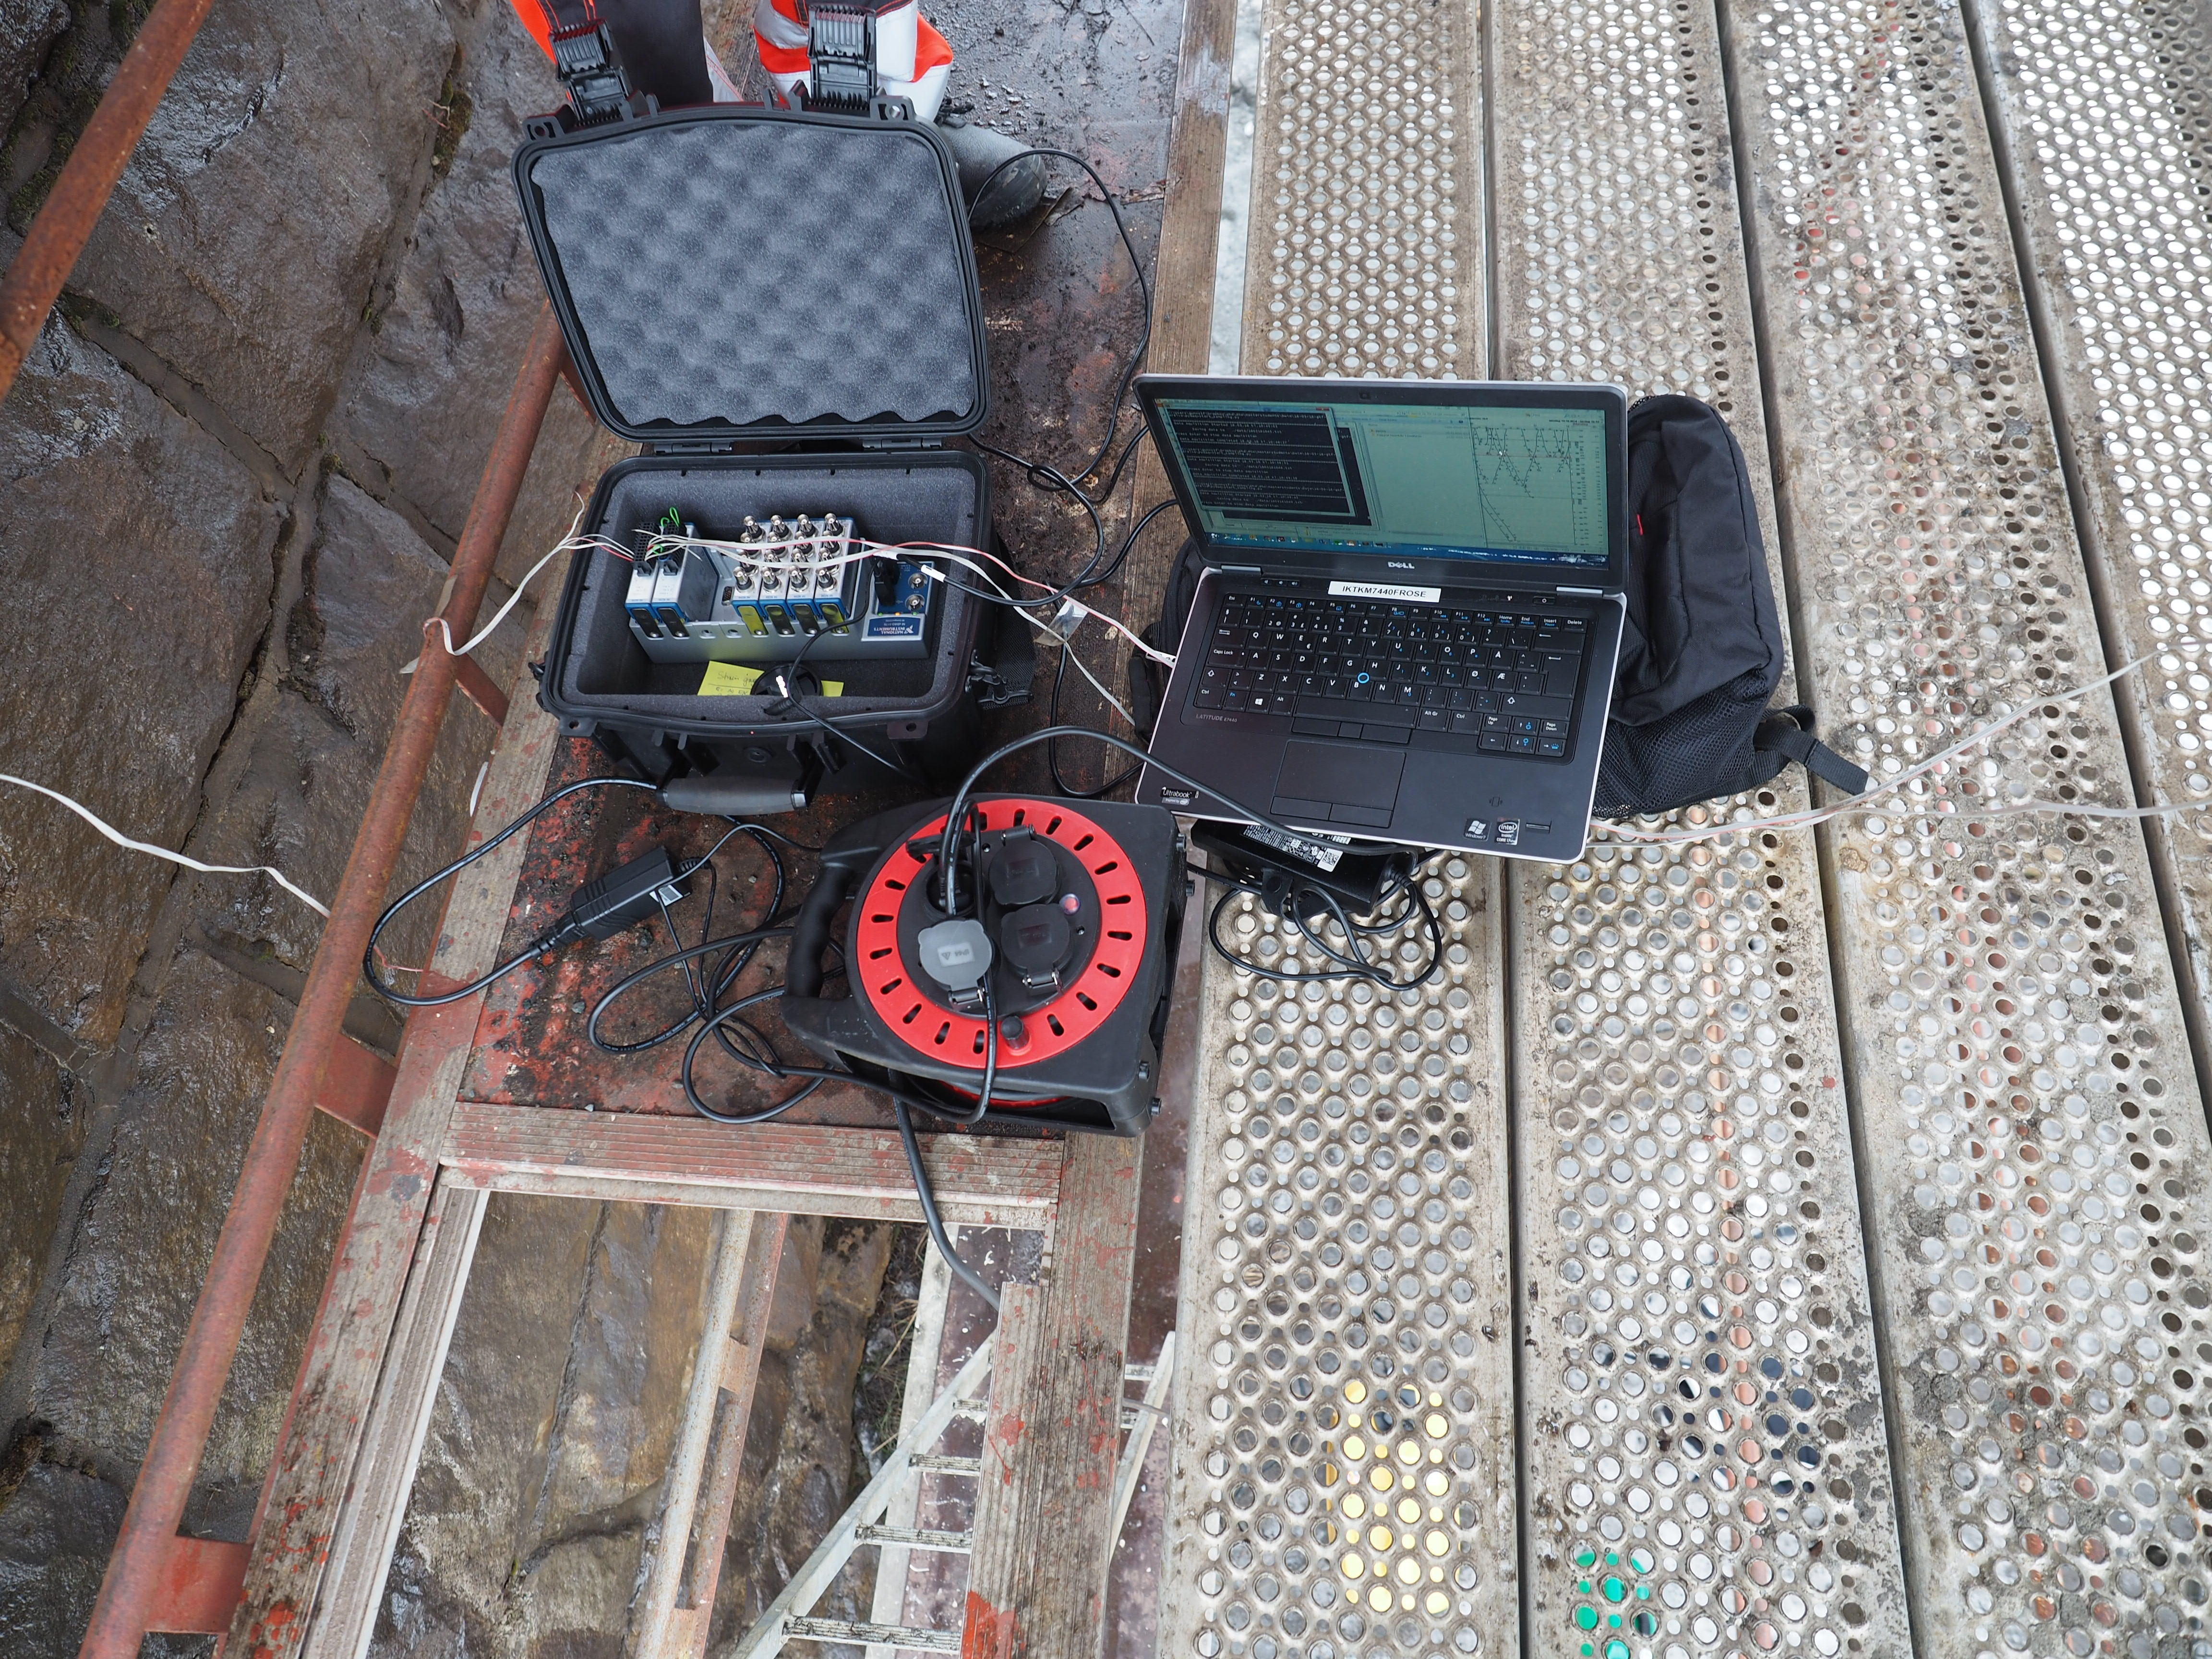
\includegraphics[width=\textwidth]{figures/system_setup}
		\caption{System setup from data gathering at Lerelva}
		\label{fig:instruments}
	\end{subfigure}
	\begin{subfigure}[t]{0.49\textwidth}
    \centering
    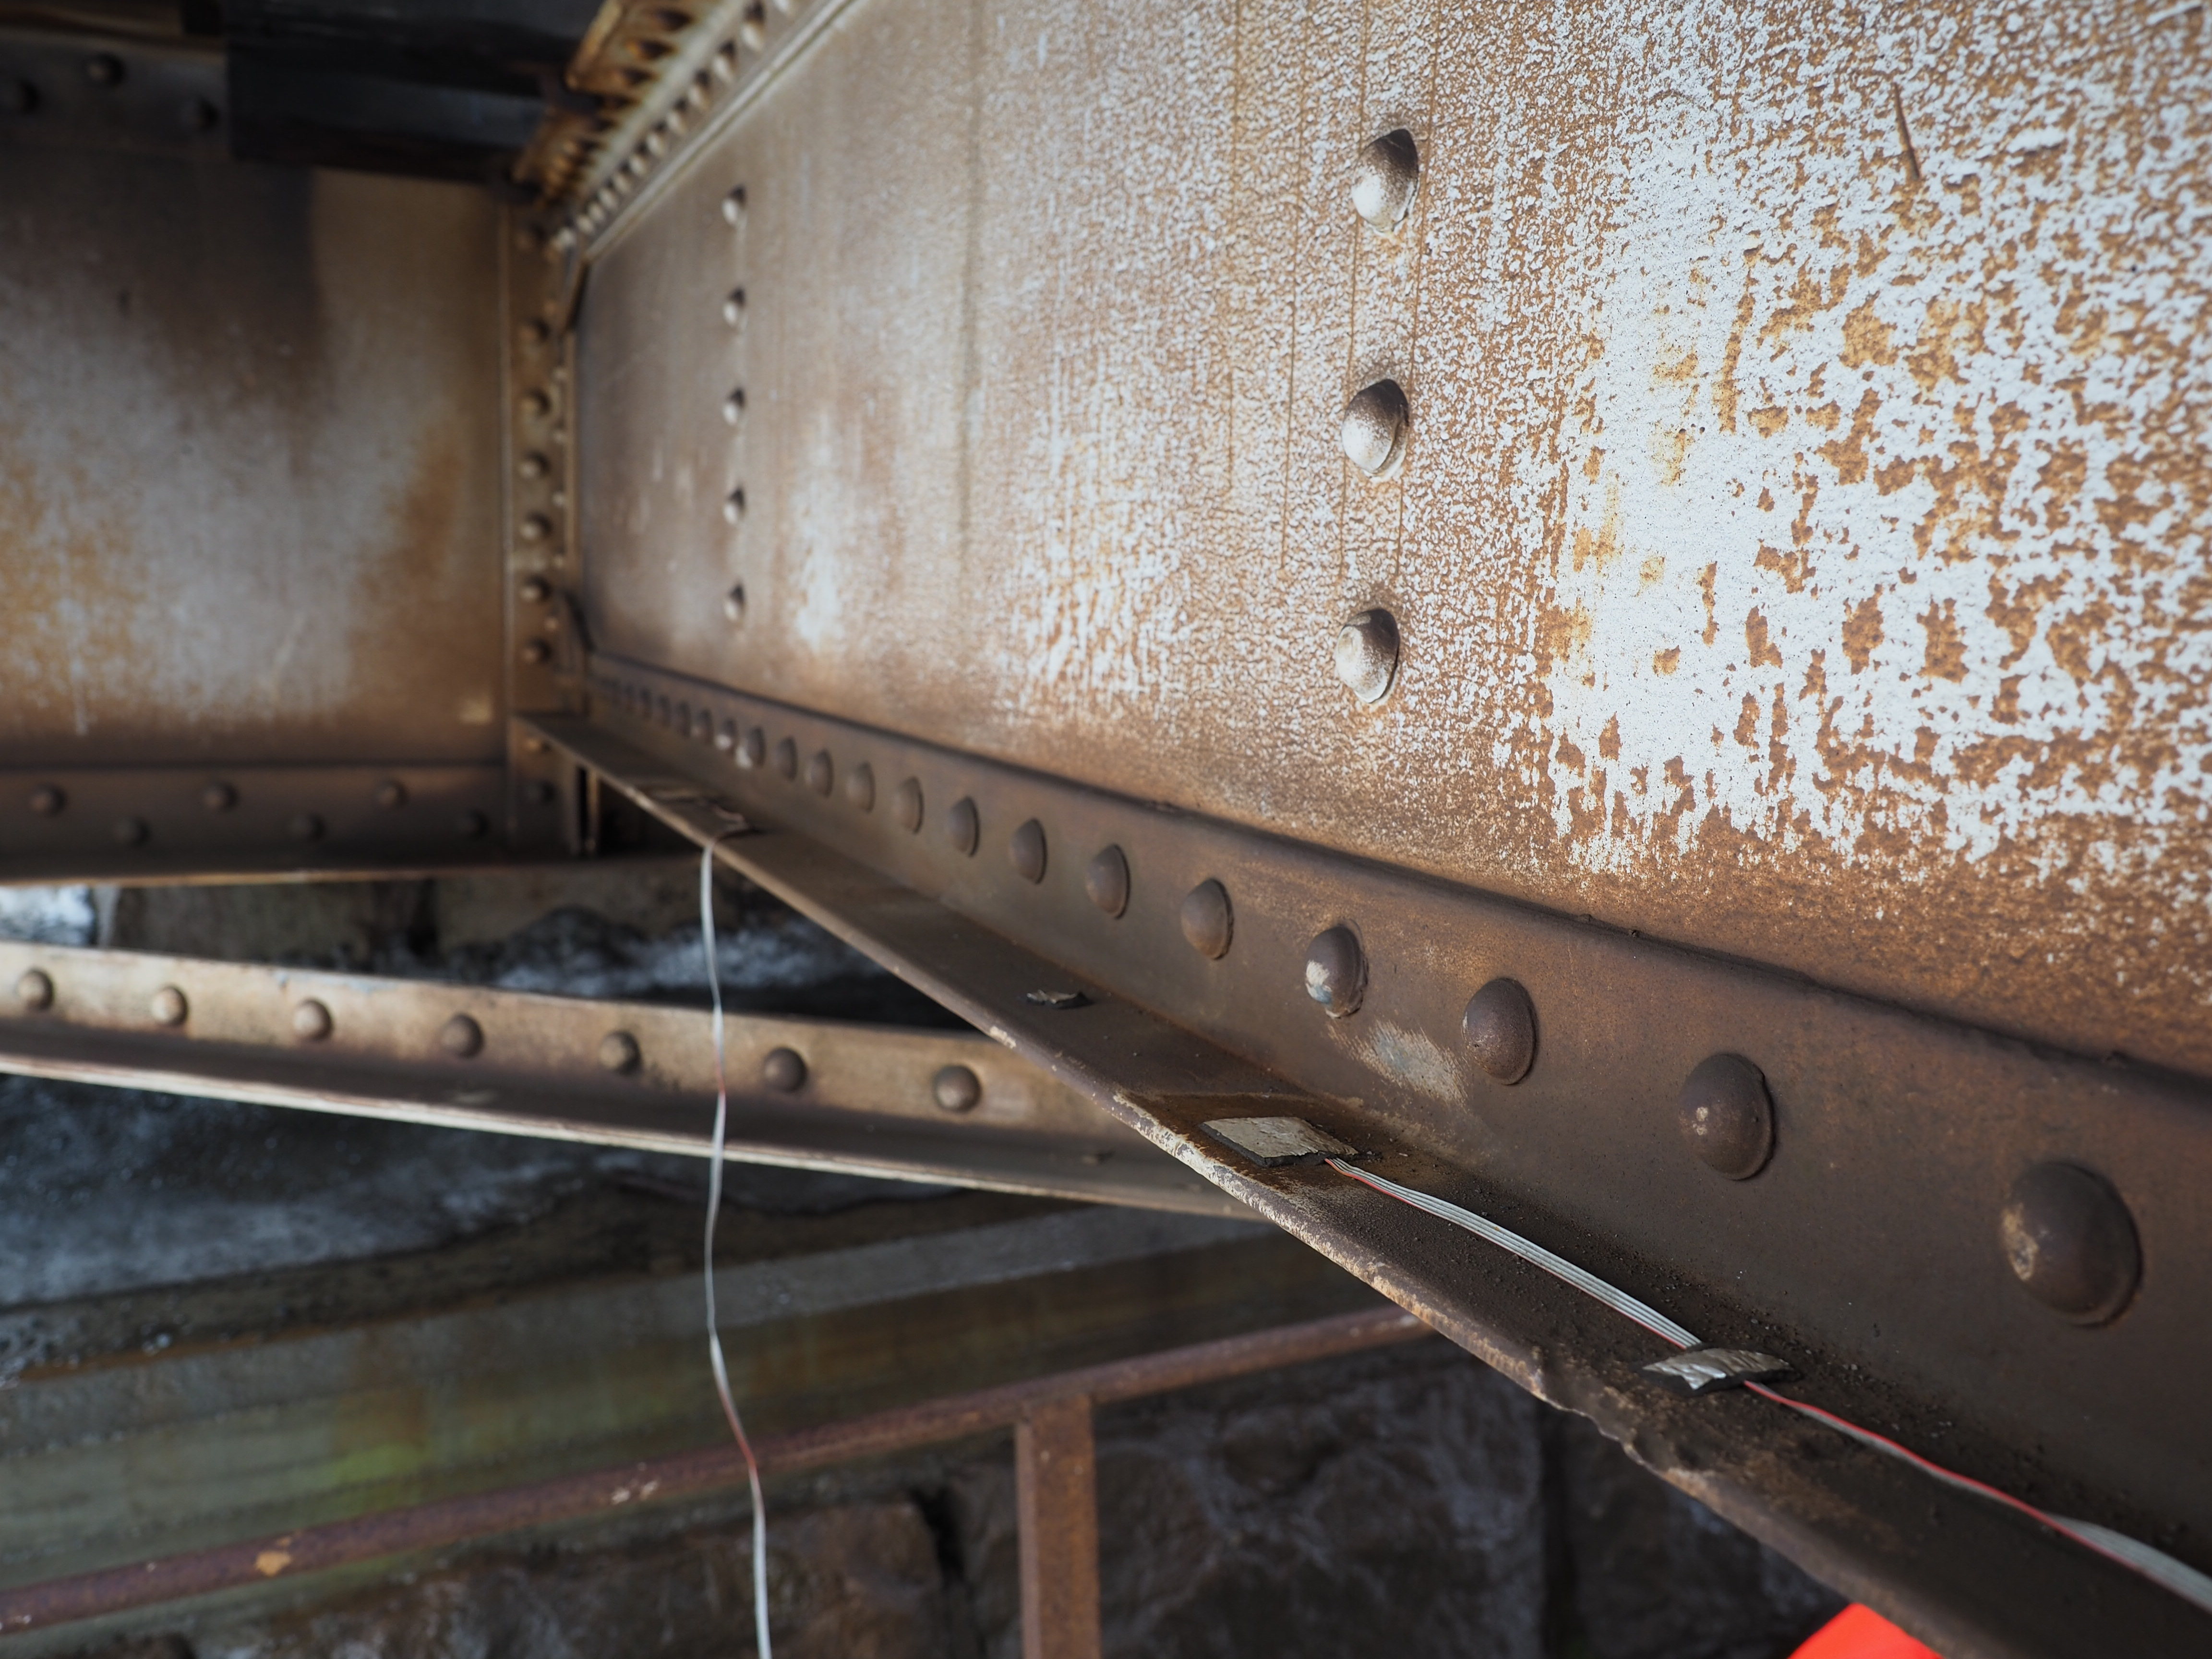
\includegraphics[width=\textwidth]{figures/sensor_placement}
		\caption{Placement of strain gauges on stringer section}
		\label{fig:strain_gauges}
	\end{subfigure}
	\caption{Instruments for aquiring strain data}
	\label{fig:system_setup}
	% 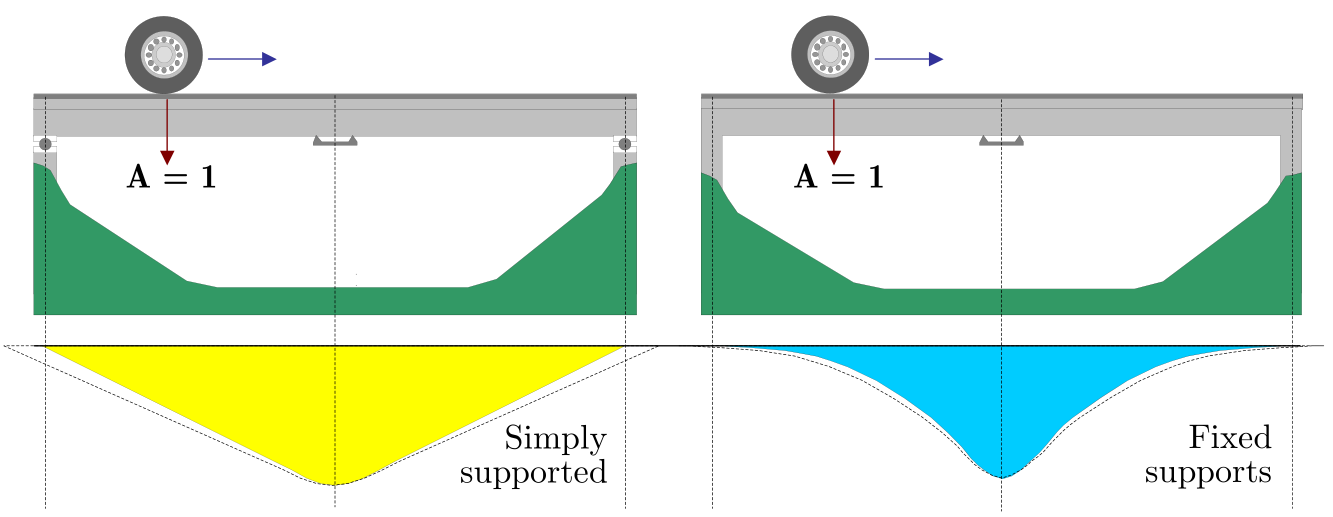
\includegraphics[scale=0.5]{figures/inflLinesQuilligan}
\end{figure}
\begin{figure}[H]
	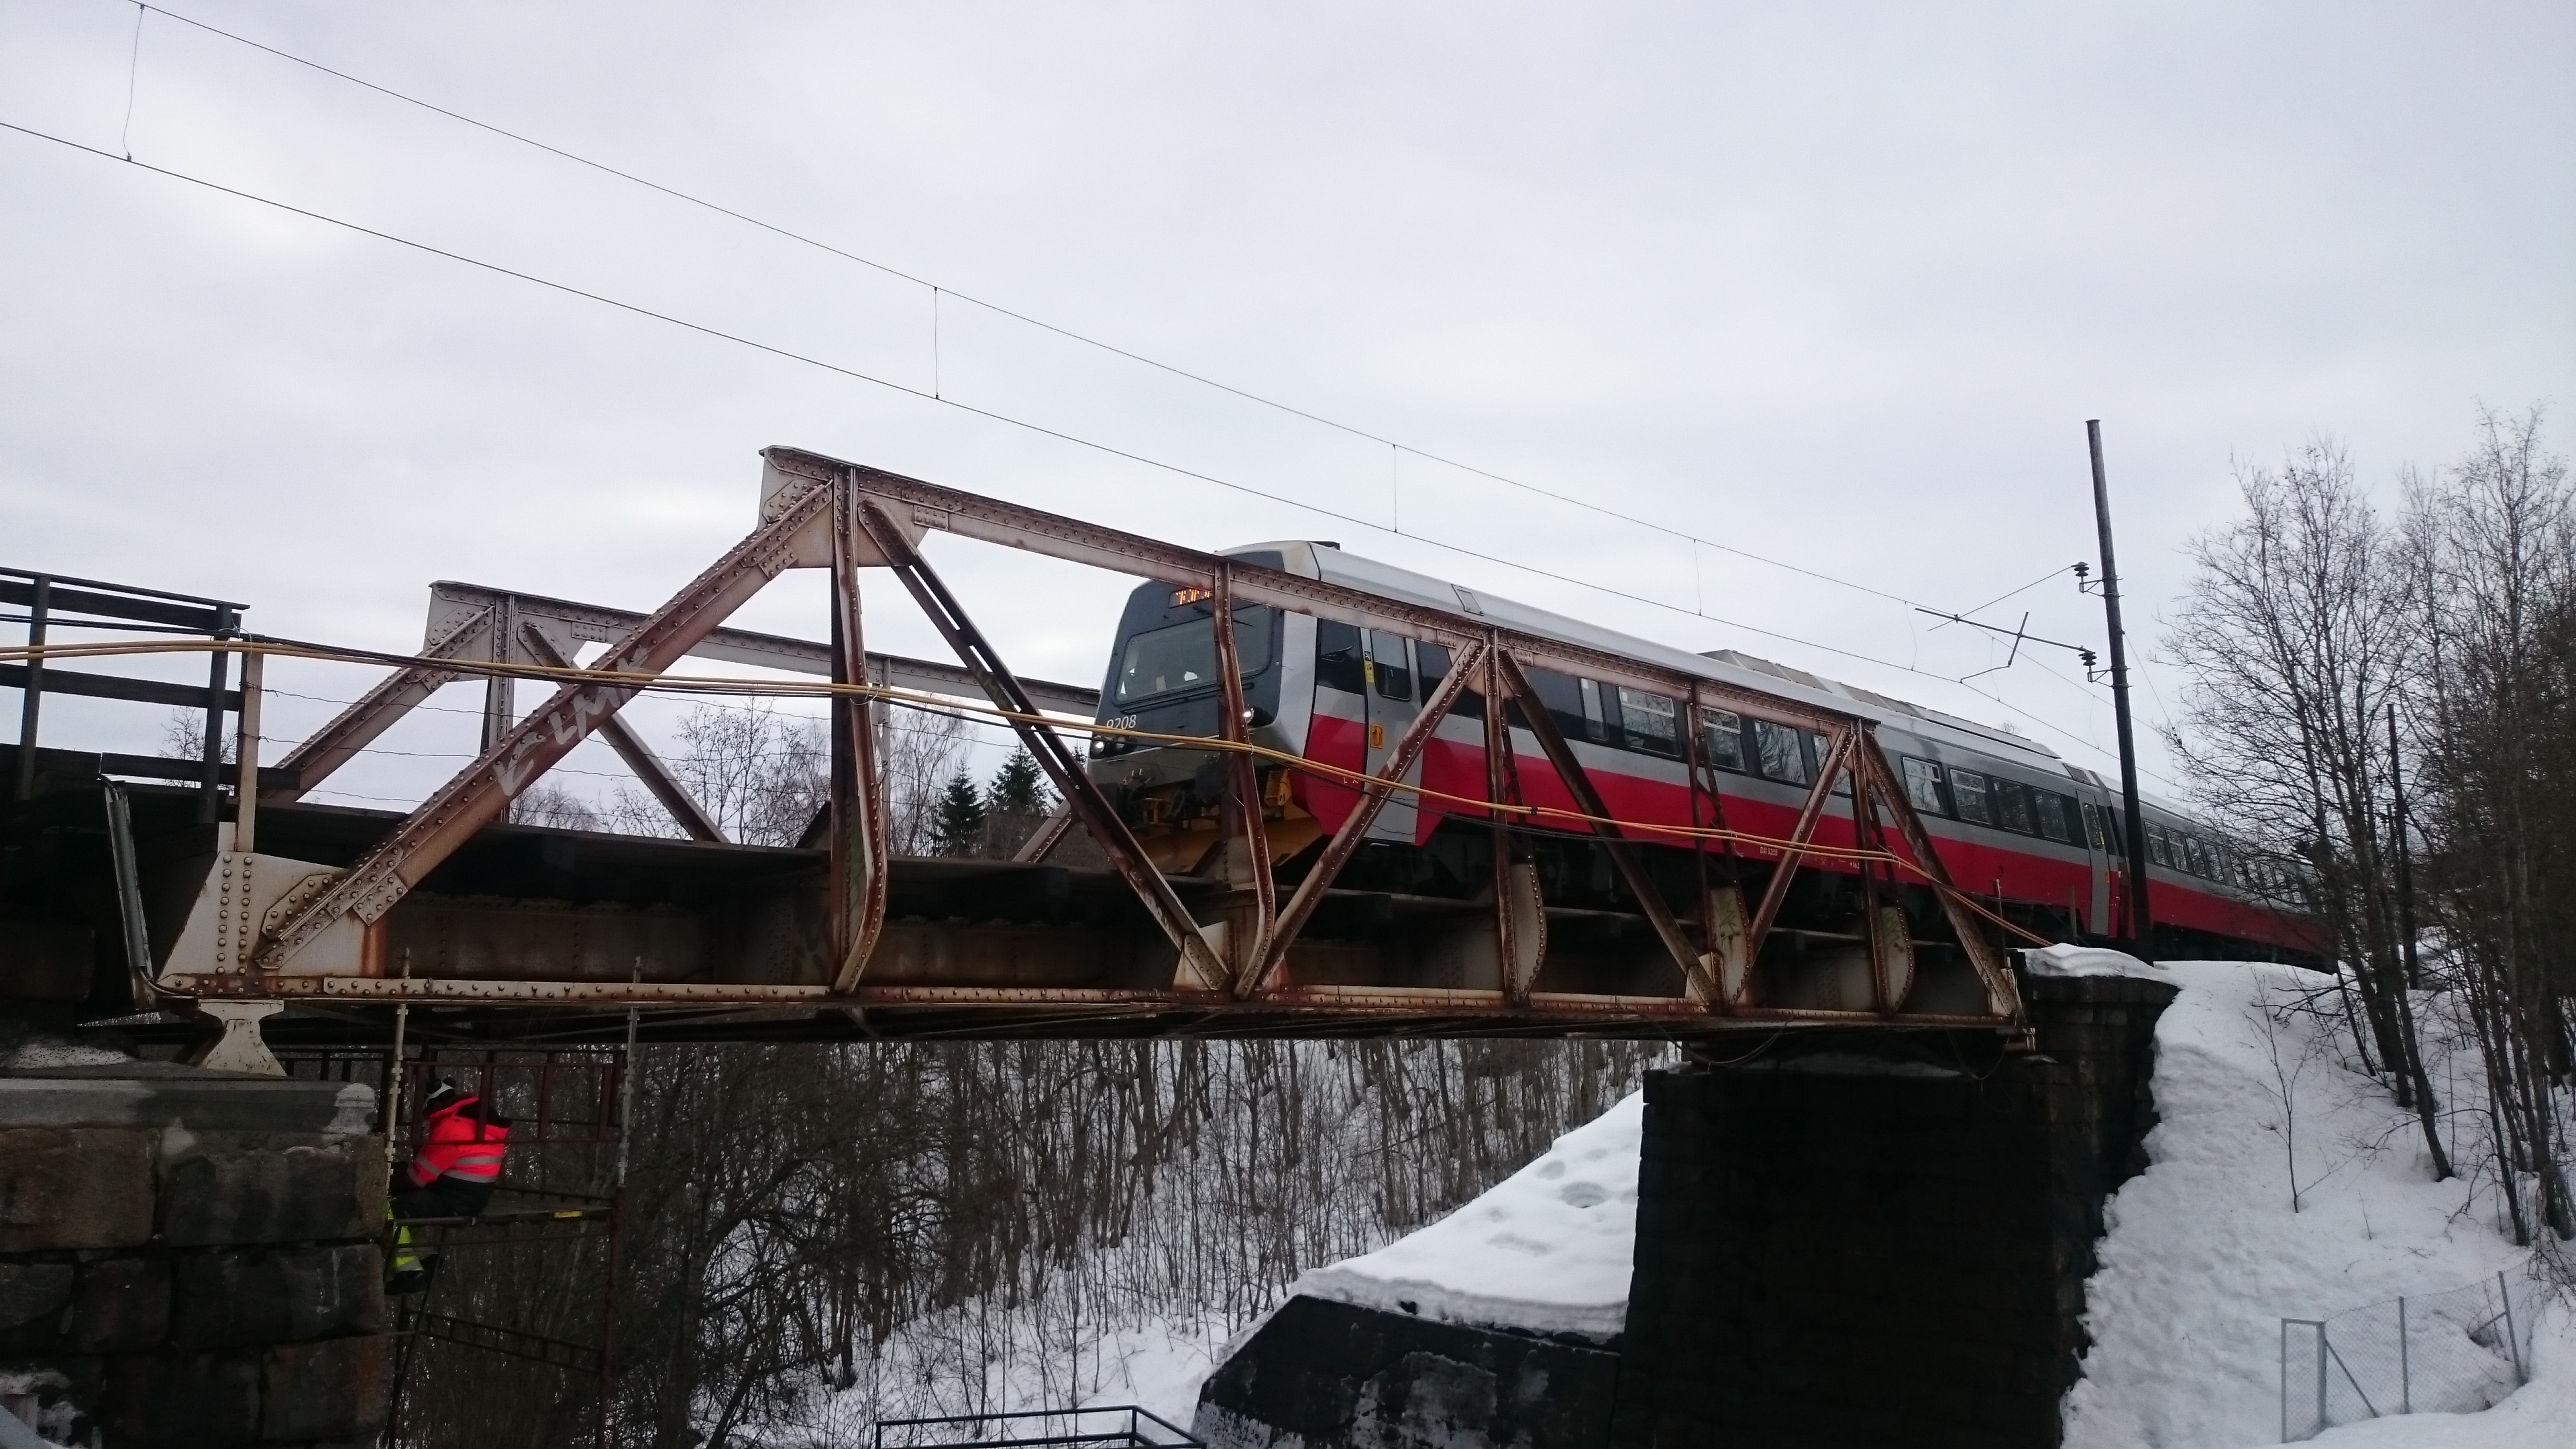
\includegraphics[width=\textwidth]{figures/train_passing.jpg}
	\caption{Lerelva bridge with a train passing over}
	\label{fig:lerelva_bridge}
\end{figure}


\subsection{Testing}
Keywords:
\begin{itemize}
\item Comparing calculated strain with measured strain
\item Perform the same test with a influence line found through the matrix method
\end{itemize}

When performing BWIM with a influence line through the matrix method, the length of the strain signal will require a influence line of a certain length. The exact position where the train begins to influence the bridge is not known due to the special conditions of the Trondheim side support and the dynamic effects in the influence line.
To use the found influence line as correctly as possible, it will be needed to place it in accordance with the provided strain signal.

\subsubsection{Using calculated influence lines}
To perform a standard BWIM calculation, the influence line needs to be aligned correctly with the strain signal, otherwise calculated Axle weights will be based on faulty calculations from solving the system

$A = I_m \textbackslash \varepsilon$
(NEEDS TO BE IN THEORY).
The first peak of the strain signal, corresponding to the first axle of the train, should occur at the same location as the peak of the influence line which should be precisely at the strain-gauge/sensor location.
Identifying the first peak of the strain signal is subject to noise which corrupts any reading of peaks in the raw strain signa. Therefore filtering of noise is needed to correctly identify the signals peaks. A trains axle spacings, as seen in \ref{appendix:nsb92} which is the train type of the readings, may consist short spacings. If the axle spacing between two axles are short compared to the bridge, they both influence the signal simoultaneously and the peaks corresponding to the two axles thus lies very close to each other. The filtering can therefore not be to hard or soft, which may result in problems when trying to automate the procedure of identifying axles.
To correctly align the strain signal and influence line, the matlab code used in this thesis first smooths the strain signal to a degree where the desired number of peaks are identifyable before using matlabs findpeaks (REFERENCE THIS) procedure to find the peak locations, like seen in figure \ref{fig:axle_peaks}.
\begin{figure}[htbp]
	\centering
	% This file was created by matlab2tikz.
%
%The latest updates can be retrieved from
%  http://www.mathworks.com/matlabcentral/fileexchange/22022-matlab2tikz-matlab2tikz
%where you can also make suggestions and rate matlab2tikz.
%
\definecolor{mycolor1}{rgb}{0.00000,0.44700,0.74100}%
\definecolor{mycolor2}{rgb}{0.85000,0.32500,0.09800}%
%
\begin{tikzpicture}

  \begin{axis}[%
    width=\textwidth,
    height=0.4\textwidth,
    at={(0\figurewidth,0\figureheight)},
    scale only axis,
    xmin=0,
    xmax=4500,
    xlabel={sensor samples},
    ymin=-5e-05,
    ymax=0.0002,
    ylabel={\varepsilon},
    axis background/.style={fill=white},
    title style={font=\bfseries},
    title={Strain signal},
    legend style={legend cell align=left,align=left,draw=white!15!black}
    ]
    \addplot [color=mycolor1,solid,forget plot]
    table[row sep=crcr]{%
    1	1.07101192055607e-06\\
    2	1.15785473831036e-06\\
    3	1.24695257432971e-06\\
    4	1.33795909976233e-06\\
    5	1.43051062004486e-06\\
    6	1.52422884868125e-06\\
    7	1.61872382133967e-06\\
    8	1.71359692420423e-06\\
    9	1.80844400939035e-06\\
    10	1.90285856936081e-06\\
    11	1.99643494167531e-06\\
    12	2.08877151507188e-06\\
    13	2.17947390782138e-06\\
    14	2.268158089514e-06\\
    15	2.35445341792965e-06\\
    16	2.43800556340617e-06\\
    17	2.51847929414396e-06\\
    18	2.5955610971638e-06\\
    19	2.6689616111522e-06\\
    20	2.73841784917348e-06\\
    21	2.80369519118109e-06\\
    22	2.86458912840487e-06\\
    23	2.92092674400533e-06\\
    24	2.97256791684727e-06\\
    25	3.01940623783136e-06\\
    26	3.06136963090643e-06\\
    27	3.09842067364385e-06\\
    28	3.13055661505934e-06\\
    29	3.15780909119241e-06\\
    30	3.18024354177006e-06\\
    31	3.19795833406382e-06\\
    32	3.21108360277028e-06\\
    33	3.21977981737855e-06\\
    34	3.22423609100969e-06\\
    35	3.2246682470972e-06\\
    36	3.22131666250271e-06\\
    37	3.21444390770554e-06\\
    38	3.20433220654909e-06\\
    39	3.19128073965453e-06\\
    40	3.17560281700575e-06\\
    41	3.15762294635929e-06\\
    42	3.13767382502496e-06\\
    43	3.11609328319061e-06\\
    44	3.0932212073238e-06\\
    45	3.0693964722678e-06\\
    46	3.04495391046257e-06\\
    47	3.02022134626329e-06\\
    48	2.99551672260636e-06\\
    49	2.97114534629135e-06\\
    50	2.94739727691906e-06\\
    51	2.92454488306264e-06\\
    52	2.9028405875642e-06\\
    53	2.88251482196242e-06\\
    54	2.8637742079848e-06\\
    55	2.84679998180184e-06\\
    56	2.8317466743631e-06\\
    57	2.81874105863844e-06\\
    58	2.80788137199758e-06\\
    59	2.7992368193022e-06\\
    60	2.79284735958379e-06\\
    61	2.78872377646215e-06\\
    62	2.78684802975203e-06\\
    63	2.7871738830346e-06\\
    64	2.78962779935979e-06\\
    65	2.79411009472477e-06\\
    66	2.80049633656153e-06\\
    67	2.80863897219052e-06\\
    68	2.81836917007551e-06\\
    69	2.82949885476947e-06\\
    70	2.84182291468976e-06\\
    71	2.85512156031882e-06\\
    72	2.86916280910931e-06\\
    73	2.88370507229044e-06\\
    74	2.89849981793621e-06\\
    75	2.91329428407222e-06\\
    76	2.92783421526998e-06\\
    77	2.94186659611012e-06\\
    78	2.95514235508501e-06\\
    79	2.96741901295683e-06\\
    80	2.9784632502808e-06\\
    81	2.98805336974028e-06\\
    82	2.99598163010627e-06\\
    83	3.00205643001963e-06\\
    84	3.00610432138358e-06\\
    85	3.00797183392982e-06\\
    86	3.00752709446612e-06\\
    87	3.00466122640742e-06\\
    88	2.9992895174123e-06\\
    89	2.99135234527266e-06\\
    90	2.98081585461111e-06\\
    91	2.96767237940475e-06\\
    92	2.95194060885043e-06\\
    93	2.933665496592e-06\\
    94	2.91291791581728e-06\\
    95	2.88979406517949e-06\\
    96	2.86441463288027e-06\\
    97	2.83692372854414e-06\\
    98	2.80748759469876e-06\\
    99	2.77629311172744e-06\\
    100	2.74354611206273e-06\\
    101	2.70946952112381e-06\\
    102	2.67430134405017e-06\\
    103	2.6382925186351e-06\\
    104	2.60170465600364e-06\\
    105	2.5648076915002e-06\\
    106	2.52787746894345e-06\\
    107	2.4911932818658e-06\\
    108	2.45503539557809e-06\\
    109	2.41968257388664e-06\\
    110	2.38540963404192e-06\\
    111	2.35248505301926e-06\\
    112	2.32116864752913e-06\\
    113	2.29170934923572e-06\\
    114	2.26434309554024e-06\\
    115	2.23929085496942e-06\\
    116	2.21675680471769e-06\\
    117	2.19692667623817e-06\\
    118	2.17996628298069e-06\\
    119	2.16602024245452e-06\\
    120	2.15521090276914e-06\\
    121	2.14763748169876e-06\\
    122	2.14337542414927e-06\\
    123	2.142475981699e-06\\
    124	2.1449660156634e-06\\
    125	2.15084802291733e-06\\
    126	2.16010038152303e-06\\
    127	2.17267781107562e-06\\
    128	2.18851204061427e-06\\
    129	2.20751267497674e-06\\
    130	2.22956824861435e-06\\
    131	2.25454745415543e-06\\
    132	2.28230053142016e-06\\
    133	2.31266080116753e-06\\
    134	2.34544632660512e-06\\
    135	2.38046168462887e-06\\
    136	2.41749982789026e-06\\
    137	2.4563440181204e-06\\
    138	2.49676981067939e-06\\
    139	2.53854707004721e-06\\
    140	2.58144199593128e-06\\
    141	2.62521913983302e-06\\
    142	2.66964339228794e-06\\
    143	2.71448192156572e-06\\
    144	2.75950604538049e-06\\
    145	2.80449301810664e-06\\
    146	2.849227717112e-06\\
    147	2.89350421309301e-06\\
    148	2.93712721071385e-06\\
    149	2.97991334739261e-06\\
    150	3.02169233973116e-06\\
    151	3.06230796882751e-06\\
    152	3.10161889752512e-06\\
    153	3.13949931452059e-06\\
    154	3.17583940215105e-06\\
    155	3.21054562659395e-06\\
    156	3.24354085111495e-06\\
    157	3.27476427487458e-06\\
    158	3.30417120163105e-06\\
    159	3.33173264443684e-06\\
    160	3.35743477410208e-06\\
    161	3.38127822077042e-06\\
    162	3.40327723940982e-06\\
    163	3.42345875134288e-06\\
    164	3.44186127512136e-06\\
    165	3.45853376106956e-06\\
    166	3.47353434467925e-06\\
    167	3.48692903471944e-06\\
    168	3.49879035242805e-06\\
    169	3.5091959384713e-06\\
    170	3.51822714449095e-06\\
    171	3.5259676260078e-06\\
    172	3.53250195321596e-06\\
    173	3.53791425578838e-06\\
    174	3.5422869172278e-06\\
    175	3.54569933354472e-06\\
    176	3.54822675013577e-06\\
    177	3.54993918968282e-06\\
    178	3.55090048270746e-06\\
    179	3.55116741111083e-06\\
    180	3.55078897362202e-06\\
    181	3.54980578058266e-06\\
    182	3.54824958392986e-06\\
    183	3.5461429466221e-06\\
    184	3.54349905409902e-06\\
    185	3.54032166869701e-06\\
    186	3.53660522627483e-06\\
    187	3.5323350726566e-06\\
    188	3.5274878358898e-06\\
    189	3.52203192876262e-06\\
    190	3.51592817454412e-06\\
    191	3.50913054751629e-06\\
    192	3.5015870185782e-06\\
    193	3.4932404950277e-06\\
    194	3.48402984258126e-06\\
    195	3.4738909767874e-06\\
    196	3.46275801023222e-06\\
    197	3.45056444133535e-06\\
    198	3.43724437009632e-06\\
    199	3.42273372587983e-06\\
    200	3.40697149222425e-06\\
    201	3.38990091372363e-06\\
    202	3.37147067026538e-06\\
    203	3.35163600430252e-06\\
    204	3.33035978739484e-06\\
    205	3.30761351296058e-06\\
    206	3.28337820303155e-06\\
    207	3.2576452177896e-06\\
    208	3.23041695776933e-06\\
    209	3.20170744982954e-06\\
    210	3.17154280930843e-06\\
    211	3.13996157217217e-06\\
    212	3.10701489242575e-06\\
    213	3.07276660156443e-06\\
    214	3.03729312838564e-06\\
    215	3.00068327903762e-06\\
    216	2.96303787873738e-06\\
    217	2.92446927812668e-06\\
    218	2.88510072873567e-06\\
    219	2.8450656334738e-06\\
    220	2.80450667944871e-06\\
    221	2.76357486171299e-06\\
    222	2.72242840774158e-06\\
    223	2.68123161353551e-06\\
    224	2.64015360321941e-06\\
    225	2.59936702484188e-06\\
    226	2.55904669578693e-06\\
    227	2.51936821175886e-06\\
    228	2.48050653370193e-06\\
    229	2.44263456725937e-06\\
    230	2.40592174945947e-06\\
    231	2.37053265724016e-06\\
    232	2.3366256521883e-06\\
    233	2.30435157547968e-06\\
    234	2.27385250646397e-06\\
    235	2.24526059765286e-06\\
    236	2.21869699804667e-06\\
    237	2.19427087578467e-06\\
    238	2.17207855003709e-06\\
    239	2.1522027408848e-06\\
    240	2.13471194466955e-06\\
    241	2.11965994095553e-06\\
    242	2.10708543583914e-06\\
    243	2.09701184489166e-06\\
    244	2.08944721753616e-06\\
    245	2.08438430316093e-06\\
    246	2.08180075777392e-06\\
    247	2.08165948852235e-06\\
    248	2.08390913195349e-06\\
    249	2.08848466049559e-06\\
    250	2.09530811030273e-06\\
    251	2.10428942235178e-06\\
    252	2.11532738751598e-06\\
    253	2.12831068527973e-06\\
    254	2.14311900481459e-06\\
    255	2.15962423631818e-06\\
    256	2.17769171983233e-06\\
    257	2.19718153821281e-06\\
    258	2.21794984052597e-06\\
    259	2.23985018189991e-06\\
    260	2.26273486576365e-06\\
    261	2.28645627446633e-06\\
    262	2.31086817447878e-06\\
    263	2.33582698274005e-06\\
    264	2.36119298121555e-06\\
    265	2.38683146737756e-06\\
    266	2.41261382909249e-06\\
    267	2.43841853329783e-06\\
    268	2.46413201885971e-06\\
    269	2.48964948511261e-06\\
    270	2.51487556878118e-06\\
    271	2.53972490325665e-06\\
    272	2.56412255553438e-06\\
    273	2.58800433749805e-06\\
    274	2.61131698964593e-06\\
    275	2.63401823677874e-06\\
    276	2.65607671659242e-06\\
    277	2.67747178352556e-06\\
    278	2.69819319158612e-06\\
    279	2.71824066120887e-06\\
    280	2.73762333646164e-06\\
    281	2.75635914010726e-06\\
    282	2.77447403513046e-06\\
    283	2.79200120234026e-06\\
    284	2.80898014454729e-06\\
    285	2.82545572858569e-06\\
    286	2.84147717708881e-06\\
    287	2.85709702243231e-06\\
    288	2.87237003562175e-06\\
    289	2.88735214312121e-06\\
    290	2.90209934469009e-06\\
    291	2.91666664522219e-06\\
    292	2.93110701335865e-06\\
    293	2.94547037928325e-06\\
    294	2.95980268360538e-06\\
    295	2.97414498860084e-06\\
    296	2.98853266231934e-06\\
    297	3.00299464519017e-06\\
    298	3.01755280777342e-06\\
    299	3.03222140722422e-06\\
    300	3.04700664887516e-06\\
    301	3.06190635810887e-06\\
    302	3.07690976640419e-06\\
    303	3.09199741410881e-06\\
    304	3.10714117113457e-06\\
    305	3.12230437540221e-06\\
    306	3.13744208749938e-06\\
    307	3.15250145866907e-06\\
    308	3.16742220793535e-06\\
    309	3.18213720291112e-06\\
    310	3.19657313763345e-06\\
    311	3.21065129964912e-06\\
    312	3.22428841753932e-06\\
    313	3.23739757913932e-06\\
    314	3.24988920988485e-06\\
    315	3.26167210001572e-06\\
    316	3.27265446879077e-06\\
    317	3.28274505342695e-06\\
    318	3.29185421017388e-06\\
    319	3.29989501477402e-06\\
    320	3.30678434954283e-06\\
    321	3.31244396443067e-06\\
    322	3.31680149969921e-06\\
    323	3.31979145825312e-06\\
    324	3.32135611621458e-06\\
    325	3.32144636099944e-06\\
    326	3.32002244694886e-06\\
    327	3.31705465947711e-06\\
    328	3.31252387970406e-06\\
    329	3.30642204264028e-06\\
    330	3.29875248317075e-06\\
    331	3.28953016532553e-06\\
    332	3.27878179161982e-06\\
    333	3.26654579057761e-06\\
    334	3.25287218190486e-06\\
    335	3.23782232013895e-06\\
    336	3.22146851895162e-06\\
    337	3.20389355961083e-06\\
    338	3.18519008839591e-06\\
    339	3.16545990899717e-06\\
    340	3.14481317710074e-06\\
    341	3.12336750544939e-06\\
    342	3.10124698866818e-06\\
    343	3.07858115803886e-06\\
    344	3.05550387718788e-06\\
    345	3.03215219031344e-06\\
    346	3.00866513510672e-06\\
    347	2.98518253291736e-06\\
    348	2.96184376896868e-06\\
    349	2.93878657554065e-06\\
    350	2.91614583100656e-06\\
    351	2.89405238743499e-06\\
    352	2.87263193915129e-06\\
    353	2.85200394419792e-06\\
    354	2.8322806100447e-06\\
    355	2.81356595418607e-06\\
    356	2.79595494942762e-06\\
    357	2.77953276272353e-06\\
    358	2.7643740953843e-06\\
    359	2.75054263134571e-06\\
    360	2.73809059898888e-06\\
    361	2.72705845073624e-06\\
    362	2.71747466333951e-06\\
    363	2.70935566043332e-06\\
    364	2.70270585756968e-06\\
    365	2.69751782858815e-06\\
    366	2.69377259083031e-06\\
    367	2.69144000539028e-06\\
    368	2.69047928731864e-06\\
    369	2.69083961948368e-06\\
    370	2.69246086264967e-06\\
    371	2.6952743532748e-06\\
    372	2.69920377957065e-06\\
    373	2.70416612551249e-06\\
    374	2.71007267175463e-06\\
    375	2.71683004179714e-06\\
    376	2.72434128127401e-06\\
    377	2.73250695789707e-06\\
    378	2.74122626939543e-06\\
    379	2.75039814674198e-06\\
    380	2.75992234005452e-06\\
    381	2.76970047480137e-06\\
    382	2.77963706632511e-06\\
    383	2.78964048121932e-06\\
    384	2.7996238347478e-06\\
    385	2.80950581427446e-06\\
    386	2.8192114195669e-06\\
    387	2.82867261183788e-06\\
    388	2.83782886448543e-06\\
    389	2.84662760966915e-06\\
    390	2.8550245761094e-06\\
    391	2.86298401479661e-06\\
    392	2.87047881064041e-06\\
    393	2.87749047945538e-06\\
    394	2.88400905105453e-06\\
    395	2.89003284059094e-06\\
    396	2.89556811163315e-06\\
    397	2.90062863576765e-06\\
    398	2.9052351547745e-06\\
    399	2.90941475260891e-06\\
    400	2.91320014552346e-06\\
    401	2.91662889967437e-06\\
    402	2.91974258645581e-06\\
    403	2.92258588658853e-06\\
    404	2.92520565464421e-06\\
    405	2.92764995620617e-06\\
    406	2.92996709024378e-06\\
    407	2.93220460950722e-06\\
    408	2.93440835182834e-06\\
    409	2.93662149513936e-06\\
    410	2.93888364879517e-06\\
    411	2.94122999340911e-06\\
    412	2.94369048088833e-06\\
    413	2.94628910568998e-06\\
    414	2.94904325751976e-06\\
    415	2.95196316476878e-06\\
    416	2.95505143694139e-06\\
    417	2.95830271318014e-06\\
    418	2.96170342275367e-06\\
    419	2.96523166205503e-06\\
    420	2.96885719127507e-06\\
    421	2.97254155248546e-06\\
    422	2.97623830940079e-06\\
    423	2.97989340761253e-06\\
    424	2.98344565260809e-06\\
    425	2.98682730142921e-06\\
    426	2.98996476240076e-06\\
    427	2.99277939598693e-06\\
    428	2.99518840852907e-06\\
    429	2.99710582939773e-06\\
    430	2.99844356096952e-06\\
    431	2.9991124898284e-06\\
    432	2.99902364670531e-06\\
    433	2.99808940191937e-06\\
    434	2.99622468247854e-06\\
    435	2.99334819654656e-06\\
    436	2.98938365069129e-06\\
    437	2.9842609452027e-06\\
    438	2.97791733281036e-06\\
    439	2.97029852634023e-06\\
    440	2.96135974122831e-06\\
    441	2.95106665935258e-06\\
    442	2.93939630134874e-06\\
    443	2.92633779543349e-06\\
    444	2.91189303176447e-06\\
    445	2.89607719250657e-06\\
    446	2.87891914903972e-06\\
    447	2.86046171912117e-06\\
    448	2.84076177829027e-06\\
    449	2.81989022135912e-06\\
    450	2.79793177145581e-06\\
    451	2.77498463575548e-06\\
    452	2.75116000873335e-06\\
    453	2.72658142548434e-06\\
    454	2.70138396935561e-06\\
    455	2.67571333981231e-06\\
    456	2.64972478808714e-06\\
    457	2.6235819297275e-06\\
    458	2.59745544463623e-06\\
    459	2.57152167658474e-06\\
    460	2.54596114544277e-06\\
    461	2.52095698650466e-06\\
    462	2.49669333228201e-06\\
    463	2.47335365296566e-06\\
    464	2.45111907242396e-06\\
    465	2.43016667709284e-06\\
    466	2.41066783541596e-06\\
    467	2.39278654560725e-06\\
    468	2.37667782942996e-06\\
    469	2.36248618941405e-06\\
    470	2.35034414646848e-06\\
    471	2.34037087419172e-06\\
    472	2.33267094534512e-06\\
    473	2.32733320493842e-06\\
    474	2.32442978319452e-06\\
    475	2.32401526032192e-06\\
    476	2.32612599354016e-06\\
    477	2.33077961519452e-06\\
    478	2.33797470907199e-06\\
    479	2.34769067021354e-06\\
    480	2.35988775162413e-06\\
    481	2.37450729933269e-06\\
    482	2.39147217526844e-06\\
    483	2.41068736542119e-06\\
    484	2.43204076876102e-06\\
    485	2.4554041604283e-06\\
    486	2.4806343207925e-06\\
    487	2.50757432013628e-06\\
    488	2.53605494697009e-06\\
    489	2.5658962663459e-06\\
    490	2.59690929302909e-06\\
    491	2.62889776302781e-06\\
    492	2.66165998578357e-06\\
    493	2.69499075830741e-06\\
    494	2.72868332172003e-06\\
    495	2.7625313400282e-06\\
    496	2.79633088055485e-06\\
    497	2.82988237524054e-06\\
    498	2.86299254205732e-06\\
    499	2.89547624601945e-06\\
    500	2.92715827974193e-06\\
    501	2.95787504418389e-06\\
    502	2.98747611111224e-06\\
    503	3.01582564992596e-06\\
    504	3.0428037027828e-06\\
    505	3.06830729345466e-06\\
    506	3.09225135699214e-06\\
    507	3.11456947908694e-06\\
    508	3.13521443596388e-06\\
    509	3.15415852769323e-06\\
    510	3.17139369996879e-06\\
    511	3.18693145162364e-06\\
    512	3.20080252743167e-06\\
    513	3.21305639804574e-06\\
    514	3.22376053122694e-06\\
    515	3.23299946079853e-06\\
    516	3.24087366199226e-06\\
    517	3.24749824401384e-06\\
    518	3.25300147271933e-06\\
    519	3.25752313823991e-06\\
    520	3.26121278419809e-06\\
    521	3.26422781680165e-06\\
    522	3.2667315135666e-06\\
    523	3.26889095268644e-06\\
    524	3.27087488511881e-06\\
    525	3.27285157228939e-06\\
    526	3.27498661290324e-06\\
    527	3.27744078270048e-06\\
    528	3.28036791108744e-06\\
    529	3.28391281841531e-06\\
    530	3.28820933726238e-06\\
    531	3.2933784404086e-06\\
    532	3.29952649727389e-06\\
    533	3.30674367943398e-06\\
    534	3.31510253443882e-06\\
    535	3.3246567455511e-06\\
    536	3.33544009321126e-06\\
    537	3.34746563203851e-06\\
    538	3.36072509501308e-06\\
    539	3.37518853417475e-06\\
    540	3.39080420474119e-06\\
    541	3.40749869701833e-06\\
    542	3.42517731787289e-06\\
    543	3.44372472088888e-06\\
    544	3.46300578166385e-06\\
    545	3.48286671204382e-06\\
    546	3.50313640447843e-06\\
    547	3.52362799512492e-06\\
    548	3.54414063187009e-06\\
    549	3.5644614311017e-06\\
    550	3.58436760486607e-06\\
    551	3.60362873802673e-06\\
    552	3.62200919320853e-06\\
    553	3.63927061969594e-06\\
    554	3.65517454107108e-06\\
    555	3.66948499524389e-06\\
    556	3.68197119965817e-06\\
    557	3.69241021386208e-06\\
    558	3.70058957132397e-06\\
    559	3.70630985235382e-06\\
    560	3.7093871702655e-06\\
    561	3.70965554348198e-06\\
    562	3.70696912714317e-06\\
    563	3.70120427891669e-06\\
    564	3.69226143512825e-06\\
    565	3.68006677500667e-06\\
    566	3.66457365276413e-06\\
    567	3.6457637793889e-06\\
    568	3.62364813839365e-06\\
    569	3.59826762231483e-06\\
    570	3.56969337947564e-06\\
    571	3.53802686337621e-06\\
    572	3.50339958003479e-06\\
    573	3.46597253164185e-06\\
    574	3.42593535797546e-06\\
    575	3.38350518012826e-06\\
    576	3.33892515418397e-06\\
    577	3.29246274552175e-06\\
    578	3.24440773738692e-06\\
    579	3.19506999021897e-06\\
    580	3.14477697093873e-06\\
    581	3.09387107393776e-06\\
    582	3.04270675785964e-06\\
    583	2.9916475243849e-06\\
    584	2.94106276710838e-06\\
    585	2.89132452020772e-06\\
    586	2.84280413792482e-06\\
    587	2.79586893690365e-06\\
    588	2.75087883413448e-06\\
    589	2.70818301363607e-06\\
    590	2.66811665505764e-06\\
    591	2.63099775709798e-06\\
    592	2.59712408802009e-06\\
    593	2.56677029458947e-06\\
    594	2.54018519949065e-06\\
    595	2.51758931568803e-06\\
    596	2.4991726043099e-06\\
    597	2.48509250046278e-06\\
    598	2.47547222894888e-06\\
    599	2.47039942918295e-06\\
    600	2.46992510571412e-06\\
    601	2.47406291767798e-06\\
    602	2.48278881726606e-06\\
    603	2.49604104393487e-06\\
    604	2.51372047761758e-06\\
    605	2.53569135068243e-06\\
    606	2.56178231483884e-06\\
    607	2.59178785565939e-06\\
    608	2.62547004389997e-06\\
    609	2.66256060939635e-06\\
    610	2.70276332002847e-06\\
    611	2.74575664510646e-06\\
    612	2.79119667958023e-06\\
    613	2.83872030273442e-06\\
    614	2.88794854253496e-06\\
    615	2.93849011456712e-06\\
    616	2.98994510257251e-06\\
    617	3.04190874597518e-06\\
    618	3.09397529850292e-06\\
    619	3.14574192107455e-06\\
    620	3.19681257154735e-06\\
    621	3.24680185371092e-06\\
    622	3.29533878807785e-06\\
    623	3.3420704675568e-06\\
    624	3.38666556200007e-06\\
    625	3.42881763688479e-06\\
    626	3.46824825300653e-06\\
    627	3.50470981602066e-06\\
    628	3.53798814694315e-06\\
    629	3.56790474729672e-06\\
    630	3.59431873543745e-06\\
    631	3.61712843369299e-06\\
    632	3.63627258925631e-06\\
    633	3.65173121527805e-06\\
    634	3.6635260422501e-06\\
    635	3.67172057353804e-06\\
    636	3.67641974276341e-06\\
    637	3.67776917462053e-06\\
    638	3.67595405459683e-06\\
    639	3.67119761691345e-06\\
    640	3.66375926377409e-06\\
    641	3.65393233266651e-06\\
    642	3.64204153196742e-06\\
    643	3.62844006841966e-06\\
    644	3.61350649314812e-06\\
    645	3.59764129572545e-06\\
    646	3.58126327836099e-06\\
    647	3.56480574453913e-06\\
    648	3.54871253835333e-06\\
    649	3.53343397234957e-06\\
    650	3.51942268288842e-06\\
    651	3.50712945284919e-06\\
    652	3.49699904191874e-06\\
    653	3.48946606472968e-06\\
    654	3.48495095673392e-06\\
    655	3.48385606692214e-06\\
    656	3.48656191533293e-06\\
    657	3.49342365174845e-06\\
    658	3.50476775006143e-06\\
    659	3.52088897053729e-06\\
    660	3.5420476196104e-06\\
    661	3.56846713396602e-06\\
    662	3.60033201250157e-06\\
    663	3.63778611636034e-06\\
    664	3.68093135362447e-06\\
    665	3.72982676147391e-06\\
    666	3.78448799470704e-06\\
    667	3.8448872255103e-06\\
    668	3.91095345530372e-06\\
    669	3.98257323541389e-06\\
    670	4.05959178927989e-06\\
    671	4.14181452491903e-06\\
    672	4.22900892251121e-06\\
    673	4.320906778241e-06\\
    674	4.41720678200285e-06\\
    675	4.51757740326528e-06\\
    676	4.62166005633644e-06\\
    677	4.72907251350812e-06\\
    678	4.83941253210767e-06\\
    679	4.95226165938152e-06\\
    680	5.06718917739172e-06\\
    681	5.18375614874896e-06\\
    682	5.30151952304205e-06\\
    683	5.42003626326988e-06\\
    684	5.53886745143896e-06\\
    685	5.6575823327644e-06\\
    686	5.77576225859741e-06\\
    687	5.89300448929604e-06\\
    688	6.00892581974384e-06\\
    689	6.12316599209015e-06\\
    690	6.23539086251657e-06\\
    691	6.34529529140439e-06\\
    692	6.45260572916037e-06\\
    693	6.55708247312568e-06\\
    694	6.65852157440996e-06\\
    695	6.7567563771268e-06\\
    696	6.85165867631949e-06\\
    697	6.94313948481762e-06\\
    698	7.03114940331559e-06\\
    699	7.115678592071e-06\\
    700	7.19675634674149e-06\\
    701	7.27445028497085e-06\\
    702	7.34886515435473e-06\\
    703	7.42014127632392e-06\\
    704	7.48845264423449e-06\\
    705	7.55400469751361e-06\\
    706	7.61703179703656e-06\\
    707	7.67779442997238e-06\\
    708	7.73657617509799e-06\\
    709	7.79368046201626e-06\\
    710	7.84942715979461e-06\\
    711	7.90414903224682e-06\\
    712	7.95818809839208e-06\\
    713	8.01189193752863e-06\\
    714	8.06560997884404e-06\\
    715	8.1196898155454e-06\\
    716	8.17447358312818e-06\\
    717	8.23029444061717e-06\\
    718	8.28747319241278e-06\\
    719	8.3463150867752e-06\\
    720	8.40710682499173e-06\\
    721	8.47011381292191e-06\\
    722	8.53557768392383e-06\\
    723	8.60371411916116e-06\\
    724	8.67471098800788e-06\\
    725	8.74872682773735e-06\\
    726	8.82588967794484e-06\\
    727	8.90629628124621e-06\\
    728	8.99001165776077e-06\\
    729	9.07706905676839e-06\\
    730	9.16747028477232e-06\\
    731	9.26118640504468e-06\\
    732	9.35815879962645e-06\\
    733	9.45830058074162e-06\\
    734	9.56149833471068e-06\\
    735	9.66761417775147e-06\\
    736	9.77648809957929e-06\\
    737	9.8879405674988e-06\\
    738	1.00017753607531e-05\\
    739	1.01177826022959e-05\\
    740	1.02357419529056e-05\\
    741	1.0355425930695e-05\\
    742	1.0476603317606e-05\\
    743	1.05990426134345e-05\\
    744	1.07225154973163e-05\\
    745	1.08468002564332e-05\\
    746	1.09716851419692e-05\\
    747	1.10969716130581e-05\\
    748	1.12224774306177e-05\\
    749	1.13480395645368e-05\\
    750	1.14735168796709e-05\\
    751	1.15987925684796e-05\\
    752	1.17237763008794e-05\\
    753	1.18484060649719e-05\\
    754	1.19726496756926e-05\\
    755	1.20965059320872e-05\\
    756	1.22200054078129e-05\\
    757	1.23432108635474e-05\\
    758	1.24662172742152e-05\\
    759	1.25891514682778e-05\\
    760	1.27121713807194e-05\\
    761	1.28354649257563e-05\\
    762	1.29592484996536e-05\\
    763	1.30837651283003e-05\\
    764	1.32092822783226e-05\\
    765	1.33360893544698e-05\\
    766	1.34644949097261e-05\\
    767	1.35948235980611e-05\\
    768	1.37274129028767e-05\\
    769	1.38626096770136e-05\\
    770	1.40007665326055e-05\\
    771	1.41422381210872e-05\\
    772	1.42873773452521e-05\\
    773	1.44365315463859e-05\\
    774	1.45900387101746e-05\\
    775	1.4748223735265e-05\\
    776	1.49113948080657e-05\\
    777	1.50798399265865e-05\\
    778	1.52538236148528e-05\\
    779	1.54335838676949e-05\\
    780	1.56193293635187e-05\\
    781	1.58112369800384e-05\\
    782	1.60094496449081e-05\\
    783	1.6214074549772e-05\\
    784	1.64251817524794e-05\\
    785	1.66428031881349e-05\\
    786	1.68669321053028e-05\\
    787	1.70975229391169e-05\\
    788	1.73344916282974e-05\\
    789	1.75777163782042e-05\\
    790	1.78270388671104e-05\\
    791	1.80822658879075e-05\\
    792	1.83431714125236e-05\\
    793	1.86094990614821e-05\\
    794	1.88809649563233e-05\\
    795	1.91572609280897e-05\\
    796	1.94380580508098e-05\\
    797	1.97230104649261e-05\\
    798	2.0011759451977e-05\\
    799	2.03039377185771e-05\\
    800	2.05991738449012e-05\\
    801	2.0897096850491e-05\\
    802	2.11973408283073e-05\\
    803	2.14995495965628e-05\\
    804	2.18033813170167e-05\\
    805	2.21085130281107e-05\\
    806	2.24146450415748e-05\\
    807	2.2721505151948e-05\\
    808	2.30288526098305e-05\\
    809	2.33364818116067e-05\\
    810	2.36442256608412e-05\\
    811	2.39519585595209e-05\\
    812	2.42595989907895e-05\\
    813	2.45671116587393e-05\\
    814	2.4874509155181e-05\\
    815	2.51818531280362e-05\\
    816	2.54892549310683e-05\\
    817	2.57968757400124e-05\\
    818	2.61049261257557e-05\\
    819	2.64136650809704e-05\\
    820	2.67233985024836e-05\\
    821	2.70344771375918e-05\\
    822	2.73472940084578e-05\\
    823	2.76622813345746e-05\\
    824	2.79799069790058e-05\\
    825	2.83006704496335e-05\\
    826	2.86250984919154e-05\\
    827	2.89537403146036e-05\\
    828	2.92871624944587e-05\\
    829	2.96259436101492e-05\\
    830	2.9970668659205e-05\\
    831	3.03219233150537e-05\\
    832	3.06802880837694e-05\\
    833	3.10463324221682e-05\\
    834	3.14206088802615e-05\\
    835	3.18036473318128e-05\\
    836	3.21959493568114e-05\\
    837	3.25979828390667e-05\\
    838	3.3010176840846e-05\\
    839	3.34329168145181e-05\\
    840	3.38665402085473e-05\\
    841	3.43113325219129e-05\\
    842	3.47675238571497e-05\\
    843	3.52352860177251e-05\\
    844	3.57147301904481e-05\\
    845	3.62059052480727e-05\\
    846	3.67087967012705e-05\\
    847	3.72233263227578e-05\\
    848	3.77493524596334e-05\\
    849	3.82866710429748e-05\\
    850	3.88350172965226e-05\\
    851	3.93940681389323e-05\\
    852	3.99634452666494e-05\\
    853	4.05427188970594e-05\\
    854	4.11314121442389e-05\\
    855	4.17290059924781e-05\\
    856	4.23349448258229e-05\\
    857	4.29486424652742e-05\\
    858	4.35694886590608e-05\\
    859	4.41968559656275e-05\\
    860	4.48301069637284e-05\\
    861	4.54686017193423e-05\\
    862	4.61117054350858e-05\\
    863	4.67587962044515e-05\\
    864	4.74092727905734e-05\\
    865	4.80625623473672e-05\\
    866	4.87181279998373e-05\\
    867	4.93754762001056e-05\\
    868	5.00341637763152e-05\\
    869	5.06938045930054e-05\\
    870	5.1354075743835e-05\\
    871	5.20147232006458e-05\\
    872	5.26755668467811e-05\\
    873	5.33365048272905e-05\\
    874	5.399751715411e-05\\
    875	5.46586685104853e-05\\
    876	5.53201102057319e-05\\
    877	5.59820812388639e-05\\
    878	5.66449084375912e-05\\
    879	5.73090056476253e-05\\
    880	5.79748719560678e-05\\
    881	5.86430889417962e-05\\
    882	5.93143169551366e-05\\
    883	5.9989290438624e-05\\
    884	6.06688123102138e-05\\
    885	6.13537474398286e-05\\
    886	6.20450152595094e-05\\
    887	6.27435815566026e-05\\
    888	6.34504495082533e-05\\
    889	6.41666500239078e-05\\
    890	6.48932314704715e-05\\
    891	6.56312488621248e-05\\
    892	6.63817526035094e-05\\
    893	6.71457768809715e-05\\
    894	6.79243278017299e-05\\
    895	6.87183713851598e-05\\
    896	6.95288215138014e-05\\
    897	7.03565279541569e-05\\
    898	7.12022645588196e-05\\
    899	7.20667177619229e-05\\
    900	7.29504754793238e-05\\
    901	7.38540165233078e-05\\
    902	7.47777006389345e-05\\
    903	7.57217592654542e-05\\
    904	7.66862871215139e-05\\
    905	7.76712347071949e-05\\
    906	7.86764018093048e-05\\
    907	7.97014320888417e-05\\
    908	8.07458088212161e-05\\
    909	8.18088518507247e-05\\
    910	8.28897158109904e-05\\
    911	8.39873896527055e-05\\
    912	8.51006975091174e-05\\
    913	8.6228300918386e-05\\
    914	8.73687024103072e-05\\
    915	8.85202504530472e-05\\
    916	8.96811457435769e-05\\
    917	9.08494488135315e-05\\
    918	9.20230889103731e-05\\
    919	9.31998741020989e-05\\
    920	9.43775025424352e-05\\
    921	9.555357482258e-05\\
    922	9.67256073252291e-05\\
    923	9.78910464869168e-05\\
    924	9.90472838657392e-05\\
    925	0.000100191671903379\\
    926	0.000101321540263108\\
    927	0.000102434212619171\\
    928	0.000103527023767728\\
    929	0.000104597336925397\\
    930	0.000105642561078463\\
    931	0.000106660168244002\\
    932	0.000107647710503574\\
    933	0.000108602836670776\\
    934	0.000109523308455774\\
    935	0.000110407015993023\\
    936	0.000111251992602645\\
    937	0.000112056428661376\\
    938	0.000112818684465564\\
    939	0.000113537301976346\\
    940	0.000114211015345801\\
    941	0.000114838760132478\\
    942	0.000115419681125185\\
    943	0.000115953138705153\\
    944	0.000116438713688627\\
    945	0.000116876210604446\\
    946	0.000117265659374116\\
    947	0.000117607315375223\\
    948	0.000117901657882549\\
    949	0.000118149386894953\\
    950	0.000118351418369689\\
    951	0.000118508877899361\\
    952	0.000118623092879984\\
    953	0.000118695583231455\\
    954	0.000118728050744169\\
    955	0.000118722367137228\\
    956	0.000118680560924787\\
    957	0.000118604803197268\\
    958	0.0001184973924335\\
    959	0.000118360738468141\\
    960	0.000118197345745936\\
    961	0.000118009796000454\\
    962	0.000117800730499772\\
    963	0.000117572832005159\\
    964	0.000117328806591142\\
    965	0.000117071365476243\\
    966	0.000116803207013381\\
    967	0.00011652699898718\\
    968	0.00011624536136244\\
    969	0.000115960849623705\\
    970	0.000115675938840285\\
    971	0.000115393008584304\\
    972	0.000115114328821423\\
    973	0.000114842046884858\\
    974	0.000114578175633296\\
    975	0.000114324582882416\\
    976	0.00011408298218794\\
    977	0.000113854925045766\\
    978	0.000113641794561654\\
    979	0.00011344480062949\\
    980	0.000113264976643287\\
    981	0.000113103177754057\\
    982	0.000112960080668521\\
    983	0.000112836184972574\\
    984	0.000112731815948464\\
    985	0.000112647128841075\\
    986	0.000112582114515515\\
    987	0.000112536606435588\\
    988	0.000112510288880823\\
    989	0.000112502706308548\\
    990	0.000112513273757281\\
    991	0.000112541288178423\\
    992	0.000112585940575076\\
    993	0.000112646328819775\\
    994	0.000112721471017146\\
    995	0.000112810319272974\\
    996	0.000112911773727974\\
    997	0.000113024696712757\\
    998	0.000113147926879979\\
    999	0.000113280293170654\\
    1000	0.00011342062847385\\
    1001	0.000113567782842694\\
    1002	0.000113720636134554\\
    1003	0.000113878109949548\\
    1004	0.000114039178748988\\
    1005	0.000114202880043966\\
    1006	0.000114368323554015\\
    1007	0.000114534699246403\\
    1008	0.000114701284178159\\
    1009	0.000114867448075246\\
    1010	0.000115032657596223\\
    1011	0.000115196479241233\\
    1012	0.000115358580881\\
    1013	0.00011551873189468\\
    1014	0.000115676801919655\\
    1015	0.00011583275823062\\
    1016	0.000115986661779427\\
    1017	0.000116138661940964\\
    1018	0.00011628899002377\\
    1019	0.000116437951616938\\
    1020	0.000116585917857058\\
    1021	0.000116733315710334\\
    1022	0.000116880617375519\\
    1023	0.000117028328922781\\
    1024	0.000117176978291992\\
    1025	0.000117327102781138\\
    1026	0.000117479236161452\\
    1027	0.000117633895560496\\
    1028	0.000117791568257644\\
    1029	0.000117952698538243\\
    1030	0.00011811767475311\\
    1031	0.000118286816728984\\
    1032	0.000118460363673066\\
    1033	0.000118638462710864\\
    1034	0.000118821158191269\\
    1035	0.000119008381886154\\
    1036	0.000119199944203883\\
    1037	0.000119395526526946\\
    1038	0.000119594674773709\\
    1039	0.000119796794272948\\
    1040	0.000120001146027594\\
    1041	0.000120206844431064\\
    1042	0.00012041285648579\\
    1043	0.000120618002559223\\
    1044	0.000120820958697824\\
    1045	0.00012102026050446\\
    1046	0.000121214308569435\\
    1047	0.000121401375430105\\
    1048	0.000121579614018926\\
    1049	0.000121747067544965\\
    1050	0.000121901680739475\\
    1051	0.000122041312382261\\
    1052	0.000122163749012432\\
    1053	0.000122266719714745\\
    1054	0.000122347911861358\\
    1055	0.000122404987678464\\
    1056	0.000122435601498035\\
    1057	0.000122437417547\\
    1058	0.000122408128119517\\
    1059	0.000122345471972807\\
    1060	0.000122247252783208\\
    1061	0.000122111357496872\\
    1062	0.000121935774408755\\
    1063	0.000121718610804335\\
    1064	0.000121458110000862\\
    1065	0.000121152667628765\\
    1066	0.000120800846999212\\
    1067	0.000120401393410655\\
    1068	0.000119953247255364\\
    1069	0.000119455555796534\\
    1070	0.000118907683497328\\
    1071	0.000118309220795154\\
    1072	0.000117659991227484\\
    1073	0.000116960056829445\\
    1074	0.000116209721738143\\
    1075	0.000115409533954098\\
    1076	0.000114560285226127\\
    1077	0.000113663009042343\\
    1078	0.000112718976726529\\
    1079	0.000111729691655851\\
    1080	0.000110696881632463\\
    1081	0.000109622489458006\\
    1082	0.000108508661776028\\
    1083	0.000107357736262907\\
    1084	0.000106172227262751\\
    1085	0.00010495480997582\\
    1086	0.000103708303323229\\
    1087	0.000102435651622781\\
    1088	0.000101139905221757\\
    1089	9.98242002422125e-05\\
    1090	9.84917376026622e-05\\
    1091	9.71457614869485e-05\\
    1092	9.57895374365261e-05\\
    1093	9.44263302462373e-05\\
    1094	9.30593818459339e-05\\
    1095	9.16918893509544e-05\\
    1096	9.03269834634891e-05\\
    1097	8.89677074042822e-05\\
    1098	8.76169965499201e-05\\
    1099	8.62776589452052e-05\\
    1100	8.4952356852838e-05\\
    1101	8.36435894939126e-05\\
    1102	8.23536771226239e-05\\
    1103	8.10847465672108e-05\\
    1104	7.98387183565808e-05\\
    1105	7.86172955384304e-05\\
    1106	7.74219542800768e-05\\
    1107	7.62539363278155e-05\\
    1108	7.51142433845225e-05\\
    1109	7.40036334485986e-05\\
    1110	7.29226191403433e-05\\
    1111	7.18714680246013e-05\\
    1112	7.08502049212096e-05\\
    1113	6.98586161775311e-05\\
    1114	6.88962558603596e-05\\
    1115	6.79624538078679e-05\\
    1116	6.7056325466194e-05\\
    1117	6.61767834198722e-05\\
    1118	6.53225505107459e-05\\
    1119	6.44921744263871e-05\\
    1120	6.36840436265103e-05\\
    1121	6.28964044645185e-05\\
    1122	6.21273793512626e-05\\
    1123	6.13749857994171e-05\\
    1124	6.06371561796559e-05\\
    1125	5.99117580141072e-05\\
    1126	5.91966146284439e-05\\
    1127	5.84895259814336e-05\\
    1128	5.77882894898807e-05\\
    1129	5.70907206676195e-05\\
    1130	5.63946733995769e-05\\
    1131	5.56980596758706e-05\\
    1132	5.4998868616423e-05\\
    1133	5.42951846235841e-05\\
    1134	5.35852045087114e-05\\
    1135	5.28672534484691e-05\\
    1136	5.21397996376841e-05\\
    1137	5.14014675178413e-05\\
    1138	5.06510494735846e-05\\
    1139	4.98875159038086e-05\\
    1140	4.91100235889241e-05\\
    1141	4.83179222915449e-05\\
    1142	4.75107595440061e-05\\
    1143	4.66882835926512e-05\\
    1144	4.58504444855582e-05\\
    1145	4.49973933071606e-05\\
    1146	4.41294795799091e-05\\
    1147	4.32472468695476e-05\\
    1148	4.23514266466156e-05\\
    1149	4.14429304722683e-05\\
    1150	4.05228405913015e-05\\
    1151	3.95923990292449e-05\\
    1152	3.86529953034113e-05\\
    1153	3.77061528697544e-05\\
    1154	3.67535144381805e-05\\
    1155	3.57968262984906e-05\\
    1156	3.48379218073071e-05\\
    1157	3.38787041931071e-05\\
    1158	3.29211288417692e-05\\
    1159	3.19671852288145e-05\\
    1160	3.1018878666743e-05\\
    1161	3.0078212036533e-05\\
    1162	2.91471676714714e-05\\
    1163	2.8227689559037e-05\\
    1164	2.7321666022603e-05\\
    1165	2.64309130392841e-05\\
    1166	2.5557158343406e-05\\
    1167	2.47020264568735e-05\\
    1168	2.38670247782496e-05\\
    1169	2.30535308517205e-05\\
    1170	2.22627809254188e-05\\
    1171	2.14958598959167e-05\\
    1172	2.07536927222141e-05\\
    1173	2.00370373783535e-05\\
    1174	1.93464793990344e-05\\
    1175	1.86824280574196e-05\\
    1176	1.80451141988569e-05\\
    1177	1.74345897386393e-05\\
    1178	1.68507288163365e-05\\
    1179	1.62932305837959e-05\\
    1180	1.5761623588777e-05\\
    1181	1.52552717014949e-05\\
    1182	1.4773381517228e-05\\
    1183	1.43150111547429e-05\\
    1184	1.38790803577085e-05\\
    1185	1.34643817946375e-05\\
    1186	1.30695934423087e-05\\
    1187	1.26932919281833e-05\\
    1188	1.23339666991115e-05\\
    1189	1.19900348767124e-05\\
    1190	1.16598566542491e-05\\
    1191	1.13417510856685e-05\\
    1192	1.10340121147519e-05\\
    1193	1.07349246910611e-05\\
    1194	1.04427808195532e-05\\
    1195	1.0155895392384e-05\\
    1196	9.87262165448748e-06\\
    1197	9.59136615897874e-06\\
    1198	9.31060307423168e-06\\
    1199	9.02888771155991e-06\\
    1200	8.7448691507185e-06\\
    1201	8.45730184984909e-06\\
    1202	8.16505613692486e-06\\
    1203	7.86712749110189e-06\\
    1204	7.56264453454771e-06\\
    1205	7.25087566816304e-06\\
    1206	6.93123429802515e-06\\
    1207	6.60328261322097e-06\\
    1208	6.26673388987439e-06\\
    1209	5.92145331046953e-06\\
    1210	5.56745730189026e-06\\
    1211	5.20491140979701e-06\\
    1212	4.83412674091554e-06\\
    1213	4.45555501838066e-06\\
    1214	4.0697823083336e-06\\
    1215	3.67752148839457e-06\\
    1216	3.27960354030478e-06\\
    1217	2.87696775984372e-06\\
    1218	2.470650986983e-06\\
    1219	2.06177596804309e-06\\
    1220	1.65153896929824e-06\\
    1221	1.24119676795542e-06\\
    1222	8.32053151661444e-07\\
    1223	4.25445061626686e-07\\
    1224	2.27285170535329e-08\\
    1225	-3.74735540183809e-07\\
    1226	-7.65595341754596e-07\\
    1227	-1.14852219257677e-06\\
    1228	-1.52222403936145e-06\\
    1229	-1.88545857741043e-06\\
    1230	-2.23704577037337e-06\\
    1231	-2.57587966416566e-06\\
    1232	-2.90093938384878e-06\\
    1233	-3.21129921092808e-06\\
    1234	-3.50613764811292e-06\\
    1235	-3.78474538904124e-06\\
    1236	-4.04653212166106e-06\\
    1237	-4.29103210579919e-06\\
    1238	-4.51790847779275e-06\\
    1239	-4.72695624780325e-06\\
    1240	-4.9181039684426e-06\\
    1241	-5.09141406649388e-06\\
    1242	-5.24708184267024e-06\\
    1243	-5.38543315740181e-06\\
    1244	-5.50692083344357e-06\\
    1245	-5.6121198185296e-06\\
    1246	-5.70172116325016e-06\\
    1247	-5.77652488067297e-06\\
    1248	-5.83743176486654e-06\\
    1249	-5.88543425531286e-06\\
    1250	-5.92160644312051e-06\\
    1251	-5.94709332288688e-06\\
    1252	-5.96309940094288e-06\\
    1253	-5.97087677646754e-06\\
    1254	-5.9717128165517e-06\\
    1255	-5.96691754965885e-06\\
    1256	-5.95781090407141e-06\\
    1257	-5.94570991878292e-06\\
    1258	-5.93191605392389e-06\\
    1259	-5.91770272617337e-06\\
    1260	-5.90430319175818e-06\\
    1261	-5.89289889558434e-06\\
    1262	-5.88460839985049e-06\\
    1263	-5.88047699919432e-06\\
    1264	-5.88146712210594e-06\\
    1265	-5.88844961006851e-06\\
    1266	-5.9021959567502e-06\\
    1267	-5.92337157966445e-06\\
    1268	-5.95253018613648e-06\\
    1269	-5.99010928426833e-06\\
    1270	-6.0364268780046e-06\\
    1271	-6.09167937346518e-06\\
    1272	-6.15594071156833e-06\\
    1273	-6.22916272972054e-06\\
    1274	-6.31117674313221e-06\\
    1275	-6.40169632424318e-06\\
    1276	-6.50032124693538e-06\\
    1277	-6.60654255077571e-06\\
    1278	-6.71974866959343e-06\\
    1279	-6.83923255835657e-06\\
    1280	-6.96419974266044e-06\\
    1281	-7.09377720628658e-06\\
    1282	-7.227023024309e-06\\
    1283	-7.36293664218532e-06\\
    1284	-7.50046969525721e-06\\
    1285	-7.63853725813093e-06\\
    1286	-7.77602940958222e-06\\
    1287	-7.91182299594273e-06\\
    1288	-8.04479347441791e-06\\
    1289	-8.17382671745717e-06\\
    1290	-8.29783066015105e-06\\
    1291	-8.41574667465401e-06\\
    1292	-8.52656055879842e-06\\
    1293	-8.62931303033998e-06\\
    1294	-8.72310962362043e-06\\
    1295	-8.80712989177169e-06\\
    1296	-8.88063582487835e-06\\
    1297	-8.94297940266229e-06\\
    1298	-8.99360920918414e-06\\
    1299	-9.03207604668004e-06\\
    1300	-9.05803749586106e-06\\
    1301	-9.07126138070451e-06\\
    1302	-9.07162810684919e-06\\
    1303	-9.05913185405541e-06\\
    1304	-9.0338806146968e-06\\
    1305	-8.99609508180418e-06\\
    1306	-8.94610640164662e-06\\
    1307	-8.88435281713131e-06\\
    1308	-8.81137523928636e-06\\
    1309	-8.7278117946737e-06\\
    1310	-8.63439140665166e-06\\
    1311	-8.53192647786476e-06\\
    1312	-8.42130475010334e-06\\
    1313	-8.30348042564722e-06\\
    1314	-8.17946464131905e-06\\
    1315	-8.05031539265658e-06\\
    1316	-7.91712701080175e-06\\
    1317	-7.78101929886e-06\\
    1318	-7.64312643755919e-06\\
    1319	-7.50458577201233e-06\\
    1320	-7.36652659224179e-06\\
    1321	-7.2300590198521e-06\\
    1322	-7.09626311184816e-06\\
    1323	-6.96617829010416e-06\\
    1324	-6.84079320142247e-06\\
    1325	-6.72103610852158e-06\\
    1326	-6.6077659067027e-06\\
    1327	-6.50176385443296e-06\\
    1328	-6.40372609870231e-06\\
    1329	-6.31425706785254e-06\\
    1330	-6.23386379571622e-06\\
    1331	-6.16295123142594e-06\\
    1332	-6.10181857926897e-06\\
    1333	-6.05065670255711e-06\\
    1334	-6.00954661477162e-06\\
    1335	-5.97845907032388e-06\\
    1336	-5.95725525627088e-06\\
    1337	-5.94568857532854e-06\\
    1338	-5.94340749966309e-06\\
    1339	-5.94995946431454e-06\\
    1340	-5.96479575880667e-06\\
    1341	-5.98727736565965e-06\\
    1342	-6.01668168519749e-06\\
    1343	-6.0522100773713e-06\\
    1344	-6.09299614333979e-06\\
    1345	-6.13811466238079e-06\\
    1346	-6.18659109338479e-06\\
    1347	-6.23741154478952e-06\\
    1348	-6.28953311239243e-06\\
    1349	-6.34189448107011e-06\\
    1350	-6.39342668407298e-06\\
    1351	-6.44306391226653e-06\\
    1352	-6.48975426547371e-06\\
    1353	-6.53247033893062e-06\\
    1354	-6.5702195397862e-06\\
    1355	-6.60205403154749e-06\\
    1356	-6.62708020834271e-06\\
    1357	-6.64446760581971e-06\\
    1358	-6.65345716135728e-06\\
    1359	-6.65336874298415e-06\\
    1360	-6.64360787389938e-06\\
    1361	-6.6236715877047e-06\\
    1362	-6.59315335829204e-06\\
    1363	-6.55174705770783e-06\\
    1364	-6.49924990512858e-06\\
    1365	-6.43556438024036e-06\\
    1366	-6.36069908471263e-06\\
    1367	-6.27476854598906e-06\\
    1368	-6.17799196818108e-06\\
    1369	-6.07069094533801e-06\\
    1370	-5.95328616267542e-06\\
    1371	-5.82629312136592e-06\\
    1372	-5.69031693214371e-06\\
    1373	-5.54604623213632e-06\\
    1374	-5.39424628793857e-06\\
    1375	-5.23575135588672e-06\\
    1376	-5.07145637771136e-06\\
    1377	-4.90230809615839e-06\\
    1378	-4.72929568072854e-06\\
    1379	-4.55344095831796e-06\\
    1380	-4.37578834722577e-06\\
    1381	-4.19739459567655e-06\\
    1382	-4.0193184276755e-06\\
    1383	-3.84261019964457e-06\\
    1384	-3.66830167088929e-06\\
    1385	-3.49739598951115e-06\\
    1386	-3.33085799294035e-06\\
    1387	-3.1696049188282e-06\\
    1388	-3.01449761766672e-06\\
    1389	-2.86633235321443e-06\\
    1390	-2.7258332706855e-06\\
    1391	-2.59364560574132e-06\\
    1392	-2.47032969970191e-06\\
    1393	-2.35635587813407e-06\\
    1394	-2.25210024116034e-06\\
    1395	-2.15784140456933e-06\\
    1396	-2.07375822116329e-06\\
    1397	-1.99992850188035e-06\\
    1398	-1.9363287461504e-06\\
    1399	-1.88283488080654e-06\\
    1400	-1.83922399676152e-06\\
    1401	-1.80517706269581e-06\\
    1402	-1.78028258526443e-06\\
    1403	-1.76404117592733e-06\\
    1404	-1.75587097553979e-06\\
    1405	-1.75511387937104e-06\\
    1406	-1.76104249736961e-06\\
    1407	-1.77286777730118e-06\\
    1408	-1.78974721195877e-06\\
    1409	-1.81079354601348e-06\\
    1410	-1.83508389331782e-06\\
    1411	-1.86166917162412e-06\\
    1412	-1.88958375877548e-06\\
    1413	-1.9178552725056e-06\\
    1414	-1.94551437503695e-06\\
    1415	-1.97160450373931e-06\\
    1416	-1.99519143015688e-06\\
    1417	-2.01537255175772e-06\\
    1418	-2.03128582375122e-06\\
    1419	-2.04211824224743e-06\\
    1420	-2.04711379483512e-06\\
    1421	-2.04558080030307e-06\\
    1422	-2.03689856564109e-06\\
    1423	-2.02052329558637e-06\\
    1424	-1.99599319773803e-06\\
    1425	-1.96293273457981e-06\\
    1426	-1.92105598253297e-06\\
    1427	-1.87016906732629e-06\\
    1428	-1.81017165441927e-06\\
    1429	-1.74105748285335e-06\\
    1430	-1.66291394063769e-06\\
    1431	-1.57592068949953e-06\\
    1432	-1.4803473564469e-06\\
    1433	-1.37655031900891e-06\\
    1434	-1.26496862013567e-06\\
    1435	-1.14611905746961e-06\\
    1436	-1.02059049995216e-06\\
    1437	-8.89037492422702e-07\\
    1438	-7.5217321592285e-07\\
    1439	-6.10761877769058e-07\\
    1440	-4.65610611038932e-07\\
    1441	-3.17560967870569e-07\\
    1442	-1.67480094862579e-07\\
    1443	-1.62516818382542e-08\\
    1444	1.35233222721005e-07\\
    1445	2.86085435183688e-07\\
    1446	4.3542680470589e-07\\
    1447	5.82399231930741e-07\\
    1448	7.26173446577445e-07\\
    1449	8.65957454776226e-07\\
    1450	1.00100457063613e-06\\
    1451	1.13062095103053e-06\\
    1452	1.25417255789645e-06\\
    1453	1.37109147841762e-06\\
    1454	1.480881540233e-06\\
    1455	1.58312316620991e-06\\
    1456	1.6774774212702e-06\\
    1457	1.76368921217414e-06\\
    1458	1.84158960996562e-06\\
    1459	1.91109727387087e-06\\
    1460	1.97221896472951e-06\\
    1461	2.02504914542577e-06\\
    1462	2.06976867518143e-06\\
    1463	2.10664261387816e-06\\
    1464	2.13601716169488e-06\\
    1465	2.15831576818813e-06\\
    1466	2.17403445341562e-06\\
    1467	2.18373639172331e-06\\
    1468	2.18804581629781e-06\\
    1469	2.18764130945857e-06\\
    1470	2.18324854985429e-06\\
    1471	2.17563259317535e-06\\
    1472	2.16558976764177e-06\\
    1473	2.15393926933271e-06\\
    1474	2.14151454534151e-06\\
    1475	2.12915455475405e-06\\
    1476	2.11769499852611e-06\\
    1477	2.1079596094739e-06\\
    1478	2.10075159279248e-06\\
    1479	2.0968453057828e-06\\
    1480	2.09697826282206e-06\\
    1481	2.10184354808686e-06\\
    1482	2.1120827141592e-06\\
    1483	2.12827923947198e-06\\
    1484	2.15095261162792e-06\\
    1485	2.18055309701877e-06\\
    1486	2.21745724994961e-06\\
    1487	2.26196420670834e-06\\
    1488	2.31429280179945e-06\\
    1489	2.3745795349594e-06\\
    1490	2.44287740868908e-06\\
    1491	2.51915564695755e-06\\
    1492	2.60330029655427e-06\\
    1493	2.69511570338061e-06\\
    1494	2.79432684687622e-06\\
    1495	2.9005825068645e-06\\
    1496	3.01345922846147e-06\\
    1497	3.13246604242154e-06\\
    1498	3.25704989046693e-06\\
    1499	3.3866016978547e-06\\
    1500	3.52046302874394e-06\\
    1501	3.6579332539121e-06\\
    1502	3.79827715508666e-06\\
    1503	3.94073288567036e-06\\
    1504	4.08452020398242e-06\\
    1505	4.2288488923588e-06\\
    1506	4.37292727357584e-06\\
    1507	4.5159707351044e-06\\
    1508	4.6572101716762e-06\\
    1509	4.79590025754964e-06\\
    1510	4.93132746168815e-06\\
    1511	5.06281772179543e-06\\
    1512	5.18974369675507e-06\\
    1513	5.3115315214624e-06\\
    1514	5.42766699327098e-06\\
    1515	5.53770112524078e-06\\
    1516	5.64125500802393e-06\\
    1517	5.73802392946907e-06\\
    1518	5.82778070881062e-06\\
    1519	5.91037821053755e-06\\
    1520	5.98575101163579e-06\\
    1521	6.05391620477004e-06\\
    1522	6.11497332902821e-06\\
    1523	6.16910342899953e-06\\
    1524	6.21656725209965e-06\\
    1525	6.25770260309929e-06\\
    1526	6.29292088366249e-06\\
    1527	6.3227028532636e-06\\
    1528	6.34759365604171e-06\\
    1529	6.36819716587901e-06\\
    1530	6.38516970917801e-06\\
    1531	6.39921323138349e-06\\
    1532	6.41106797918259e-06\\
    1533	6.42150477545609e-06\\
    1534	6.43131696839359e-06\\
    1535	6.44131213967828e-06\\
    1536	6.45230365925497e-06\\
    1537	6.46510217589284e-06\\
    1538	6.48050713352003e-06\\
    1539	6.49929840313339e-06\\
    1540	6.52222811897465e-06\\
    1541	6.55001280562248e-06\\
    1542	6.58332587969976e-06\\
    1543	6.62279060606674e-06\\
    1544	6.66897358369953e-06\\
    1545	6.72237883099157e-06\\
    1546	6.78344253401354e-06\\
    1547	6.85252851439244e-06\\
    1548	6.92992446599135e-06\\
    1549	7.01583900156521e-06\\
    1550	7.11039954211742e-06\\
    1551	7.21365107287282e-06\\
    1552	7.32555578070957e-06\\
    1553	7.44599357864356e-06\\
    1554	7.5747635136362e-06\\
    1555	7.71158604469216e-06\\
    1556	7.85610616902783e-06\\
    1557	8.00789736511646e-06\\
    1558	8.16646631275065e-06\\
    1559	8.33125834199172e-06\\
    1560	8.50166355509217e-06\\
    1561	8.67702355825777e-06\\
    1562	8.85663873354123e-06\\
    1563	9.03977597529583e-06\\
    1564	9.22567681053084e-06\\
    1565	9.41356581825282e-06\\
    1566	9.60265925949655e-06\\
    1567	9.79217382728255e-06\\
    1568	9.9813354242136e-06\\
    1569	1.01693878748568e-05\\
    1570	1.03556014804628e-05\\
    1571	1.05392813249441e-05\\
    1572	1.07197752433583e-05\\
    1573	1.08964813674056e-05\\
    1574	1.1068855166608e-05\\
    1575	1.12364159088646e-05\\
    1576	1.13987524699105e-05\\
    1577	1.15555284278004e-05\\
    1578	1.17064863858105e-05\\
    1579	1.18514514750492e-05\\
    1580	1.19903339964875e-05\\
    1581	1.21231311709981e-05\\
    1582	1.22499279752204e-05\\
    1583	1.23708970505637e-05\\
    1584	1.24862976823207e-05\\
    1585	1.2596473855587e-05\\
    1586	1.27018514043716e-05\\
    1587	1.28029342798383e-05\\
    1588	1.29002999729332e-05\\
    1589	1.29945941356429e-05\\
    1590	1.30865244536812e-05\\
    1591	1.31768538314487e-05\\
    1592	1.32663929575424e-05\\
    1593	1.33559923258553e-05\\
    1594	1.34465337933036e-05\\
    1595	1.35389217604083e-05\\
    1596	1.36340740652618e-05\\
    1597	1.37329126848009e-05\\
    1598	1.38363543397263e-05\\
    1599	1.3945301100846e-05\\
    1600	1.40606310950418e-05\\
    1601	1.41831894084688e-05\\
    1602	1.43137792829869e-05\\
    1603	1.44531536992177e-05\\
    1604	1.46020074360304e-05\\
    1605	1.47609696917274e-05\\
    1606	1.49305973467651e-05\\
    1607	1.51113689415594e-05\\
    1608	1.53036794358532e-05\\
    1609	1.55078358083308e-05\\
    1610	1.57240535467327e-05\\
    1611	1.59524540697384e-05\\
    1612	1.61930631124278e-05\\
    1613	1.64458100973145e-05\\
    1614	1.67105285028475e-05\\
    1615	1.69869572310211e-05\\
    1616	1.7274742965413e-05\\
    1617	1.75734435006916e-05\\
    1618	1.78825320145139e-05\\
    1619	1.820140224286e-05\\
    1620	1.85293745103475e-05\\
    1621	1.88657025580102e-05\\
    1622	1.92095811025327e-05\\
    1623	1.95601540530756e-05\\
    1624	1.99165233046981e-05\\
    1625	2.02777580210628e-05\\
    1626	2.0642904313655e-05\\
    1627	2.10109952202294e-05\\
    1628	2.13810608816615e-05\\
    1629	2.1752138813868e-05\\
    1630	2.21232841699998e-05\\
    1631	2.2493579887728e-05\\
    1632	2.28621466171357e-05\\
    1633	2.32281523265074e-05\\
    1634	2.35908214861468e-05\\
    1635	2.39494437342372e-05\\
    1636	2.4303381933648e-05\\
    1637	2.46520795344381e-05\\
    1638	2.49950671635612e-05\\
    1639	2.5331968370868e-05\\
    1640	2.56625044688554e-05\\
    1641	2.59864984126513e-05\\
    1642	2.63038776763481e-05\\
    1643	2.66146760919247e-05\\
    1644	2.69190346275102e-05\\
    1645	2.7217201092544e-05\\
    1646	2.75095287683678e-05\\
    1647	2.7796473973824e-05\\
    1648	2.80785925864302e-05\\
    1649	2.83565355505276e-05\\
    1650	2.86310434143545e-05\\
    1651	2.89029399481668e-05\\
    1652	2.91731249052007e-05\\
    1653	2.94425659963553e-05\\
    1654	2.9712290157864e-05\\
    1655	2.99833741988317e-05\\
    1656	3.02569349222613e-05\\
    1657	3.05341188190033e-05\\
    1658	3.08160914388669e-05\\
    1659	3.11040265468832e-05\\
    1660	3.13990951753618e-05\\
    1661	3.17024546838965e-05\\
    1662	3.20152379398386e-05\\
    1663	3.23385427309525e-05\\
    1664	3.26734215200013e-05\\
    1665	3.30208716478967e-05\\
    1666	3.33818260878074e-05\\
    1667	3.37571448473004e-05\\
    1668	3.41476071092298e-05\\
    1669	3.45539041947519e-05\\
    1670	3.49766334236079e-05\\
    1671	3.54162929377469e-05\\
    1672	3.58732775445609e-05\\
    1673	3.6347875625559e-05\\
    1674	3.68402671453324e-05\\
    1675	3.7350522784255e-05\\
    1676	3.78786042066535e-05\\
    1677	3.84243654642747e-05\\
    1678	3.89875555229046e-05\\
    1679	3.95678218880735e-05\\
    1680	4.01647152940407e-05\\
    1681	4.07776954088105e-05\\
    1682	4.1406137496908e-05\\
    1683	4.20493399711616e-05\\
    1684	4.27065327549001e-05\\
    1685	4.33768863668942e-05\\
    1686	4.40595216331402e-05\\
    1687	4.47535199223058e-05\\
    1688	4.54579337953938e-05\\
    1689	4.61717979550259e-05\\
    1690	4.68941403757427e-05\\
    1691	4.76239934939272e-05\\
    1692	4.83604053344099e-05\\
    1693	4.91024504505397e-05\\
    1694	4.98492405555128e-05\\
    1695	5.05999347250418e-05\\
    1696	5.13537490550079e-05\\
    1697	5.21099656625423e-05\\
    1698	5.28679409249859e-05\\
    1699	5.36271128583339e-05\\
    1700	5.43870075450122e-05\\
    1701	5.51472445300869e-05\\
    1702	5.5907541115181e-05\\
    1703	5.666771549038e-05\\
    1704	5.74276886561306e-05\\
    1705	5.8187485099469e-05\\
    1706	5.89472322017384e-05\\
    1707	5.97071583681304e-05\\
    1708	6.04675898827972e-05\\
    1709	6.12289465067832e-05\\
    1710	6.19917358494825e-05\\
    1711	6.27565465576131e-05\\
    1712	6.35240403786592e-05\\
    1713	6.42949431682488e-05\\
    1714	6.50700349228615e-05\\
    1715	6.58501389304914e-05\\
    1716	6.663611014228e-05\\
    1717	6.74288228775931e-05\\
    1718	6.82291579834273e-05\\
    1719	6.90379895763018e-05\\
    1720	6.98561715008452e-05\\
    1721	7.06845236440385e-05\\
    1722	7.15238182474812e-05\\
    1723	7.23747663620412e-05\\
    1724	7.32380045898241e-05\\
    1725	7.41140822574993e-05\\
    1726	7.50034491626861e-05\\
    1727	7.59064440313008e-05\\
    1728	7.6823283818554e-05\\
    1729	7.77540539796848e-05\\
    1730	7.86986998285803e-05\\
    1731	7.96570190932347e-05\\
    1732	8.06286557666088e-05\\
    1733	8.16130953399755e-05\\
    1734	8.26096614933583e-05\\
    1735	8.36175143043267e-05\\
    1736	8.46356500223029e-05\\
    1737	8.56629024408152e-05\\
    1738	8.66979458849252e-05\\
    1739	8.77392998155126e-05\\
    1740	8.87853350363722e-05\\
    1741	8.98342814743115e-05\\
    1742	9.08842374867934e-05\\
    1743	9.19331806362963e-05\\
    1744	9.29789798556154e-05\\
    1745	9.40194089139657e-05\\
    1746	9.5052161080093e-05\\
    1747	9.6074864865814e-05\\
    1748	9.70851007216109e-05\\
    1749	9.80804185452263e-05\\
    1750	9.90583558547509e-05\\
    1751	0.000100016456469578\\
    1752	0.000100952289535898\\
    1753	0.000101863468728205\\
    1754	0.000102747671454639\\
    1755	0.000103602657891967\\
    1756	0.000104426289675586\\
    1757	0.000105216548071237\\
    1758	0.000105971551457982\\
    1759	0.000106689571956633\\
    1760	0.000107369051043927\\
    1761	0.000108008614000555\\
    1762	0.000108607083050332\\
    1763	0.000109163489058537\\
    1764	0.000109677081669394\\
    1765	0.000110147337775952\\
    1766	0.000110573968229938\\
    1767	0.000110956922714499\\
    1768	0.000111296392718929\\
    1769	0.000111592812571313\\
    1770	0.000111846858502468\\
    1771	0.000112059445732296\\
    1772	0.000112231723587693\\
    1773	0.000112365068679147\\
    1774	0.000112461076181083\\
    1775	0.00011252154927859\\
    1776	0.000112548486860283\\
    1777	0.000112544069553539\\
    1778	0.000112510644214013\\
    1779	0.000112450706996103\\
    1780	0.000112366885144605\\
    1781	0.000112261917660269\\
    1782	0.000112138635002944\\
    1783	0.000111999938005601\\
    1784	0.000111848776180525\\
    1785	0.000111688125605306\\
    1786	0.000111520966580875\\
    1787	0.00011135026125672\\
    1788	0.000111178931419405\\
    1789	0.000111009836639785\\
    1790	0.000110845752971653\\
    1791	0.000110689352390139\\
    1792	0.000110543183151972\\
    1793	0.000110409651251783\\
    1794	0.000110291003139007\\
    1795	0.000110189309848786\\
    1796	0.000110106452687614\\
    1797	0.000110044110600434\\
    1798	0.000110003749330658\\
    1799	0.000109986612468235\\
    1800	0.000109993714463561\\
    1801	0.000110025835667001\\
    1802	0.000110083519435043\\
    1803	0.000110167071325016\\
    1804	0.000110276560380873\\
    1805	0.000110411822493103\\
    1806	0.000110572465796454\\
    1807	0.000110757878050106\\
    1808	0.000110967235926326\\
    1809	0.000111199516115723\\
    1810	0.000111453508140113\\
    1811	0.000111727828747911\\
    1812	0.000112020937751979\\
    1813	0.000112331155156266\\
    1814	0.00011265667940528\\
    1815	0.000112995606579842\\
    1816	0.000113345950353497\\
    1817	0.000113705662516757\\
    1818	0.000114072653870896\\
    1819	0.000114444815289484\\
    1820	0.000114820038744227\\
    1821	0.000115196238092003\\
    1822	0.000115571369422273\\
    1823	0.000115943450768222\\
    1824	0.000116310580991115\\
    1825	0.000116670957655271\\
    1826	0.00011702289372079\\
    1827	0.000117364832892551\\
    1828	0.000117695363476988\\
    1829	0.00011801323061256\\
    1830	0.000118317346755622\\
    1831	0.000118606800320288\\
    1832	0.000118880862388874\\
    1833	0.00011913899142824\\
    1834	0.000119380835966855\\
    1835	0.000119606235207326\\
    1836	0.000119815217569333\\
    1837	0.000120007997178284\\
    1838	0.000120184968335172\\
    1839	0.00012034669802307\\
    1840	0.000120493916525127\\
    1841	0.000120627506247678\\
    1842	0.000120748488859987\\
    1843	0.000120858010878997\\
    1844	0.000120957327843109\\
    1845	0.000121047787233332\\
    1846	0.000121130810312927\\
    1847	0.000121207873067866\\
    1848	0.000121280486439835\\
    1849	0.000121350176051138\\
    1850	0.000121418461626539\\
    1851	0.000121486836320766\\
    1852	0.000121556746162144\\
    1853	0.000121629569822434\\
    1854	0.0001217065989206\\
    1855	0.000121789019063813\\
    1856	0.00012187789182259\\
    1857	0.000121974137828663\\
    1858	0.000122078521173959\\
    1859	0.000122191635277149\\
    1860	0.0001223138903706\\
    1861	0.000122445502745445\\
    1862	0.000122586485875951\\
    1863	0.000122736643526635\\
    1864	0.000122895564926743\\
    1865	0.000123062622077017\\
    1866	0.000123236969233274\\
    1867	0.000123417544590405\\
    1868	0.000123603074169211\\
    1869	0.000123792077887168\\
    1870	0.000123982877773008\\
    1871	0.000124173608264106\\
    1872	0.000124362228505274\\
    1873	0.000124546536547874\\
    1874	0.000124724185329372\\
    1875	0.000124892700295778\\
    1876	0.000125049498512924\\
    1877	0.000125191909097546\\
    1878	0.000125317194785616\\
    1879	0.000125422574443654\\
    1880	0.000125505246318735\\
    1881	0.000125562411814907\\
    1882	0.000125591299577681\\
    1883	0.00012558918966425\\
    1884	0.000125553437575247\\
    1885	0.000125481497924075\\
    1886	0.000125370947522235\\
    1887	0.000125219507663564\\
    1888	0.000125025065396862\\
    1889	0.00012478569358498\\
    1890	0.000124499669558949\\
    1891	0.000124165492188114\\
    1892	0.000123781897201337\\
    1893	0.000123347870610008\\
    1894	0.000122862660100793\\
    1895	0.000122325784284439\\
    1896	0.000121737039706577\\
    1897	0.000121096505546908\\
    1898	0.000120404545954415\\
    1899	0.000119661809988036\\
    1900	0.000118869229154314\\
    1901	0.000118028012555783\\
    1902	0.000117139639686008\\
    1903	0.000116205850929017\\
    1904	0.000115228635842223\\
    1905	0.000114210219322537\\
    1906	0.00011315304577511\\
    1907	0.000112059761422739\\
    1908	0.000110933194911339\\
    1909	0.000109776336382752\\
    1910	0.000108592315200495\\
    1911	0.000107384376526593\\
    1912	0.000106155856958386\\
    1913	0.000104910159442931\\
    1914	0.000103650727693354\\
    1915	0.000102381020336092\\
    1916	0.000101104485020463\\
    1917	9.98245327222138e-05\\
    1918	9.85445124708562e-05\\
    1919	9.72676867264984e-05\\
    1920	9.59972076256957e-05\\
    1921	9.47360943075927e-05\\
    1922	9.34872115213796e-05\\
    1923	9.22532497039504e-05\\
    1924	9.10367067027476e-05\\
    1925	8.98398713032216e-05\\
    1926	8.86648087033002e-05\\
    1927	8.75133480588871e-05\\
    1928	8.63870722048913e-05\\
    1929	8.52873096358009e-05\\
    1930	8.42151288085562e-05\\
    1931	8.31713348086597e-05\\
    1932	8.21564683982813e-05\\
    1933	8.11708074427977e-05\\
    1934	8.02143706899574e-05\\
    1935	7.92869238538966e-05\\
    1936	7.83879879347627e-05\\
    1937	7.75168496839346e-05\\
    1938	7.66725741049557e-05\\
    1939	7.58540188615185e-05\\
    1940	7.50598504463261e-05\\
    1941	7.42885619485789e-05\\
    1942	7.35384922433489e-05\\
    1943	7.28078464133407e-05\\
    1944	7.20947172026228e-05\\
    1945	7.13971072929492e-05\\
    1946	7.07129521863544e-05\\
    1947	7.00401434728737e-05\\
    1948	6.93765522595392e-05\\
    1949	6.87200525362735e-05\\
    1950	6.80685442559296e-05\\
    1951	6.74199759095039e-05\\
    1952	6.67723663834264e-05\\
    1953	6.61238258937567e-05\\
    1954	6.5472575801995e-05\\
    1955	6.48169671289699e-05\\
    1956	6.41554975967512e-05\\
    1957	6.34868270436384e-05\\
    1958	6.28097910738345e-05\\
    1959	6.21234128212705e-05\\
    1960	6.14269127260109e-05\\
    1961	6.07197162415779e-05\\
    1962	6.00014594121581e-05\\
    1963	5.92719922798171e-05\\
    1964	5.85313801033321e-05\\
    1965	5.77799023918352e-05\\
    1966	5.70180497779491e-05\\
    1967	5.62465187762659e-05\\
    1968	5.54662044936628e-05\\
    1969	5.4678191377875e-05\\
    1970	5.38837421097399e-05\\
    1971	5.30842847624277e-05\\
    1972	5.22813983675832e-05\\
    1973	5.1476797043477e-05\\
    1974	5.06723128538477e-05\\
    1975	4.98698775779773e-05\\
    1976	4.90715035825711e-05\\
    1977	4.82792639941103e-05\\
    1978	4.74952723764355e-05\\
    1979	4.67216621223487e-05\\
    1980	4.59605657699479e-05\\
    1981	4.52140944542256e-05\\
    1982	4.44843177021676e-05\\
    1983	4.37732437752144e-05\\
    1984	4.30828007565443e-05\\
    1985	4.24148185722607e-05\\
    1986	4.17710121253208e-05\\
    1987	4.11529657090209e-05\\
    1988	4.05621188531881e-05\\
    1989	3.99997537410489e-05\\
    1990	3.9466984318224e-05\\
    1991	3.89647471975835e-05\\
    1992	3.84937944449841e-05\\
    1993	3.80546883113826e-05\\
    1994	3.76477979566774e-05\\
    1995	3.72732981900744e-05\\
    1996	3.69311702310183e-05\\
    1997	3.6621204473979e-05\\
    1998	3.63430052198511e-05\\
    1999	3.60959973166125e-05\\
    2000	3.58794346324105e-05\\
    2001	3.5692410265581e-05\\
    2002	3.55338683784653e-05\\
    2003	3.54026175254288e-05\\
    2004	3.52973453303905e-05\\
    2005	3.52166343555763e-05\\
    2006	3.51589789912647e-05\\
    2007	3.51228031861109e-05\\
    2008	3.51064788293193e-05\\
    2009	3.51083445895716e-05\\
    2010	3.51267250112658e-05\\
    2011	3.51599496663296e-05\\
    2012	3.5206372159657e-05\\
    2013	3.52643887880863e-05\\
    2014	3.53324566567609e-05\\
    2015	3.54091110626705e-05\\
    2016	3.54929819630664e-05\\
    2017	3.55828093562402e-05\\
    2018	3.5677457413706e-05\\
    2019	3.57759272160533e-05\\
    2020	3.58773679594757e-05\\
    2021	3.59810865160982e-05\\
    2022	3.60865552485457e-05\\
    2023	3.61934179975462e-05\\
    2024	3.63014941805571e-05\\
    2025	3.64107809592368e-05\\
    2026	3.65214534538631e-05\\
    2027	3.66338630033116e-05\\
    2028	3.67485334897374e-05\\
    2029	3.68661557674484e-05\\
    2030	3.69875802554002e-05\\
    2031	3.71138077720832e-05\\
    2032	3.72459787101053e-05\\
    2033	3.73853606653112e-05\\
    2034	3.75333346516372e-05\\
    2035	3.76913800479087e-05\\
    2036	3.78610584362933e-05\\
    2037	3.80439965039746e-05\\
    2038	3.82418681896968e-05\\
    2039	3.84563762650326e-05\\
    2040	3.86892335464624e-05\\
    2041	3.89421439385524e-05\\
    2042	3.92167835106331e-05\\
    2043	3.95147818093878e-05\\
    2044	3.983770360765e-05\\
    2045	4.01870312855035e-05\\
    2046	4.05641480335133e-05\\
    2047	4.0970322059648e-05\\
    2048	4.14066919712721e-05\\
    2049	4.18742534915798e-05\\
    2050	4.23738476561387e-05\\
    2051	4.29061506199399e-05\\
    2052	4.34716651886746e-05\\
    2053	4.4070714170028e-05\\
    2054	4.4703435621805e-05\\
    2055	4.53697800538369e-05\\
    2056	4.60695096201058e-05\\
    2057	4.68021993165383e-05\\
    2058	4.75672401786978e-05\\
    2059	4.83638444523602e-05\\
    2060	4.91910526889032e-05\\
    2061	5.00477426967962e-05\\
    2062	5.09326402604714e-05\\
    2063	5.18443315186694e-05\\
    2064	5.27812768762224e-05\\
    2065	5.37418263063155e-05\\
    2066	5.47242358847725e-05\\
    2067	5.57266853839743e-05\\
    2068	5.67472967418188e-05\\
    2069	5.77841532107831e-05\\
    2070	5.88353189837731e-05\\
    2071	5.98988590871471e-05\\
    2072	6.09728593271401e-05\\
    2073	6.20554460739533e-05\\
    2074	6.31448056680482e-05\\
    2075	6.42392032356883e-05\\
    2076	6.53370007055124e-05\\
    2077	6.64366738248414e-05\\
    2078	6.75368279834785e-05\\
    2079	6.86362126638671e-05\\
    2080	6.97337343495208e-05\\
    2081	7.08284677385217e-05\\
    2082	7.19196651254448e-05\\
    2083	7.30067638331637e-05\\
    2084	7.40893915954235e-05\\
    2085	7.51673698116887e-05\\
    2086	7.62407146173199e-05\\
    2087	7.73096357344627e-05\\
    2088	7.83745330918572e-05\\
    2089	7.94359912249126e-05\\
    2090	8.04947714905959e-05\\
    2091	8.15518021547086e-05\\
    2092	8.26081664317497e-05\\
    2093	8.36650885795612e-05\\
    2094	8.47239181720772e-05\\
    2095	8.57861126935546e-05\\
    2096	8.68532186164232e-05\\
    2097	8.79268511421769e-05\\
    2098	8.90086728003302e-05\\
    2099	9.01003711142431e-05\\
    2100	9.12036355543956e-05\\
    2101	9.23201340093634e-05\\
    2102	9.34514890121725e-05\\
    2103	9.45992539648341e-05\\
    2104	9.57648896065727e-05\\
    2105	9.69497409715652e-05\\
    2106	9.81550150798436e-05\\
    2107	9.93817596004065e-05\\
    2108	0.000100630842718563\\
    2109	0.000101902934430138\\
    2110	0.000103198489473473\\
    2111	0.000104517732096314\\
    2112	0.000105860642838685\\
    2113	0.000107226947495023\\
    2114	0.000108616108399181\\
    2115	0.000110027318154702\\
    2116	0.000111459495910152\\
    2117	0.000112911286255525\\
    2118	0.00011438106079101\\
    2119	0.000115866922393936\\
    2120	0.000117366712183854\\
    2121	0.000118878019159506\\
    2122	0.000120398192455408\\
    2123	0.000121924356139898\\
    2124	0.000123453426451267\\
    2125	0.00012498213134409\\
    2126	0.000126507032194437\\
    2127	0.000128024547490447\\
    2128	0.000129530978314071\\
    2129	0.000131022535400784\\
    2130	0.000132495367546996\\
    2131	0.000133945591119817\\
    2132	0.000135369320411095\\
    2133	0.000136762698567172\\
    2134	0.000138121928817868\\
    2135	0.000139443305722845\\
    2136	0.000140723246150746\\
    2137	0.000141958319706461\\
    2138	0.000143145278324531\\
    2139	0.000144281084752007\\
    2140	0.000145362939652106\\
    2141	0.000146388307070558\\
    2142	0.000147354938019626\\
    2143	0.000148260891950279\\
    2144	0.000149104555900701\\
    2145	0.000149884661129198\\
    2146	0.000150600297061278\\
    2147	0.000151250922404211\\
    2148	0.000151836373307358\\
    2149	0.000152356868472806\\
    2150	0.000152813011148235\\
    2151	0.000153205787961969\\
    2152	0.000153536564588821\\
    2153	0.000153807078264221\\
    2154	0.000154019427192939\\
    2155	0.000154176056927282\\
    2156	0.000154279743817644\\
    2157	0.000154333575665415\\
    2158	0.000154340929734348\\
    2159	0.000154305448301151\\
    2160	0.000154231011949262\\
    2161	0.000154121710831009\\
    2162	0.000153981814142738\\
    2163	0.00015381573807453\\
    2164	0.000153628012510862\\
    2165	0.000153423246770789\\
    2166	0.000153206094685734\\
    2167	0.000152981219319797\\
    2168	0.000152753257641477\\
    2169	0.000152526785456816\\
    2170	0.000152306282912203\\
    2171	0.000152096100870451\\
    2172	0.00015190042845625\\
    2173	0.000151723262056879\\
    2174	0.000151568376051069\\
    2175	0.000151439295523427\\
    2176	0.000151339271203856\\
    2177	0.000151271256851191\\
    2178	0.000151237889277975\\
    2179	0.000151241471189099\\
    2180	0.000151283956981219\\
    2181	0.000151366941622608\\
    2182	0.000151491652704676\\
    2183	0.000151658945727138\\
    2184	0.00015186930264886\\
    2185	0.000152122833706198\\
    2186	0.000152419282470306\\
    2187	0.000152758034084908\\
    2188	0.0001531381265964\\
    2189	0.000153558265259509\\
    2190	0.000154016839674003\\
    2191	0.000154511943581704\\
    2192	0.000155041397128274\\
    2193	0.000155602771371385\\
    2194	0.00015619341479604\\
    2195	0.000156810481579192\\
    2196	0.000157450961329669\\
    2197	0.00015811171001581\\
    2198	0.00015878948178237\\
    2199	0.000159480961350192\\
    2200	0.000160182796687025\\
    2201	0.000160891631635687\\
    2202	0.000161604138186555\\
    2203	0.000162317048085164\\
    2204	0.00016302718347242\\
    2205	0.000163731486264507\\
    2206	0.000164427045992018\\
    2207	0.000165111125832875\\
    2208	0.000165781186591273\\
    2209	0.000166434908394827\\
    2210	0.00016707020990435\\
    2211	0.00016768526485478\\
    2212	0.000168278515771756\\
    2213	0.000168848684735707\\
    2214	0.000169394781094017\\
    2215	0.000169916106051441\\
    2216	0.000170412254099272\\
    2217	0.000170883111274513\\
    2218	0.000171328850271124\\
    2219	0.00017174992245606\\
    2220	0.000172147046873027\\
    2221	0.000172521196346259\\
    2222	0.000172873580825007\\
    2223	0.000173205628136454\\
    2224	0.00017351896234027\\
    2225	0.000173815379901616\\
    2226	0.00017409682392105\\
    2227	0.000174365356679062\\
    2228	0.000174623130769906\\
    2229	0.000174872359113623\\
    2230	0.000175115284146693\\
    2231	0.000175354146500413\\
    2232	0.000175591153481793\\
    2233	0.000175828447674469\\
    2234	0.0001760680759768\\
    2235	0.000176311959390926\\
    2236	0.000176561863870179\\
    2237	0.000176819372522924\\
    2238	0.000177085859458647\\
    2239	0.000177362465547207\\
    2240	0.000177650076344526\\
    2241	0.000177949302418013\\
    2242	0.000178260462282671\\
    2243	0.000178583568134508\\
    2244	0.000178918314541679\\
    2245	0.000179264070226015\\
    2246	0.000179619873038506\\
    2247	0.000179984428202178\\
    2248	0.000180356109864894\\
    2249	0.000180732965973238\\
    2250	0.00018111272644712\\
    2251	0.000181492814603281\\
    2252	0.000181870361744918\\
    2253	0.000182242224804332\\
    2254	0.000182605006896233\\
    2255	0.000182955080611328\\
    2256	0.000183288613853354\\
    2257	0.000183601597998049\\
    2258	0.000183889878129925\\
    2259	0.000184149185092301\\
    2260	0.000184375169068117\\
    2261	0.000184563434393671\\
    2262	0.000184709575294885\\
    2263	0.000184809212225931\\
    2264	0.000184858028483346\\
    2265	0.000184851806765042\\
    2266	0.000184786465342975\\
    2267	0.000184658093520673\\
    2268	0.00018446298605234\\
    2269	0.000184197676208739\\
    2270	0.0001838589671865\\
    2271	0.000183443961571756\\
    2272	0.00018295008858596\\
    2273	0.000182375128861221\\
    2274	0.000181717236514318\\
    2275	0.000180974958312552\\
    2276	0.000180147249750479\\
    2277	0.000179233487884174\\
    2278	0.000178233480798683\\
    2279	0.000177147473614475\\
    2280	0.00017597615096977\\
    2281	0.000174720635947234\\
    2282	0.000173382485445431\\
    2283	0.000171963682027377\\
    2284	0.000170466622310081\\
    2285	0.000168894101990045\\
    2286	0.000167249297629739\\
    2287	0.000165535745359111\\
    2288	0.000163757316673651\\
    2289	0.00016191819153644\\
    2290	0.000160022829015501\\
    2291	0.000158075935709576\\
    2292	0.000156082432234909\\
    2293	0.000154047418062524\\
    2294	0.000151976135009783\\
    2295	0.000149873929701458\\
    2296	0.000147746215324141\\
    2297	0.000145598433003398\\
    2298	0.000143436013135693\\
    2299	0.000141264337006647\\
    2300	0.000139088699023723\\
    2301	0.000136914269885007\\
    2302	0.000134746060996371\\
    2303	0.000132588890437141\\
    2304	0.000130447350759501\\
    2305	0.000128325778889433\\
    2306	0.000126228228377184\\
    2307	0.00012415844422323\\
    2308	0.000122119840481718\\
    2309	0.000120115480817621\\
    2310	0.000118148062166595\\
    2311	0.000116219901618008\\
    2312	0.000114332926612136\\
    2313	0.000112488668512343\\
    2314	0.000110688259582428\\
    2315	0.000108932433368612\\
    2316	0.000107221528455016\\
    2317	0.000105555495531357\\
    2318	0.000103933907682132\\
    2319	0.000102355973778106\\
    2320	0.000100820554823722\\
    2321	9.93261830883344e-05\\
    2322	9.78710838251827e-05\\
    2323	9.64531993599651e-05\\
    2324	9.50702153109915e-05\\
    2325	9.37195886852812e-05\\
    2326	9.23985775798587e-05\\
    2327	9.11042722049706e-05\\
    2328	8.9833626936113e-05\\
    2329	8.85834930947145e-05\\
    2330	8.7350652153086e-05\\
    2331	8.61318490578878e-05\\
    2332	8.49238253678322e-05\\
    2333	8.37233519056437e-05\\
    2334	8.2527260631356e-05\\
    2335	8.13324754537662e-05\\
    2336	8.01360417091782e-05\\
    2337	7.89351540513248e-05\\
    2338	7.77271825134002e-05\\
    2339	7.65096965222868e-05\\
    2340	7.52804866661408e-05\\
    2341	7.40375840392781e-05\\
    2342	7.27792770125692e-05\\
    2343	7.15041253030556e-05\\
    2344	7.0210971243001e-05\\
    2345	6.88989481758207e-05\\
    2346	6.75674859340374e-05\\
    2347	6.62163133823225e-05\\
    2348	6.48454580365227e-05\\
    2349	6.34552427970965e-05\\
    2350	6.20462798623109e-05\\
    2351	6.06194619126461e-05\\
    2352	5.91759506828553e-05\\
    2353	5.77171630618272e-05\\
    2354	5.62447548825502e-05\\
    2355	5.47606025849053e-05\\
    2356	5.32667829525203e-05\\
    2357	5.17655511413393e-05\\
    2358	5.02593172317598e-05\\
    2359	4.87506215480439e-05\\
    2360	4.72421089981135e-05\\
    2361	4.57365026937347e-05\\
    2362	4.42365771154227e-05\\
    2363	4.27451310881344e-05\\
    2364	4.12649608329717e-05\\
    2365	3.97988333567096e-05\\
    2366	3.83494604350497e-05\\
    2367	3.69194734371556e-05\\
    2368	3.55113992283459e-05\\
    2369	3.41276373749322e-05\\
    2370	3.27704388602295e-05\\
    2371	3.14418865038965e-05\\
    2372	3.01438772581619e-05\\
    2373	2.88781065343609e-05\\
    2374	2.76460546917354e-05\\
    2375	2.64489757978836e-05\\
    2376	2.52878887467895e-05\\
    2377	2.41635707962633e-05\\
    2378	2.30765535621341e-05\\
    2379	2.20271214818669e-05\\
    2380	2.10153127357146e-05\\
    2381	2.00409225892587e-05\\
    2382	1.91035090975142e-05\\
    2383	1.82024010878733e-05\\
    2384	1.73367083172839e-05\\
    2385	1.65053336783923e-05\\
    2386	1.57069873101288e-05\\
    2387	1.4940202450565e-05\\
    2388	1.42033528539702e-05\\
    2389	1.34946715800037e-05\\
    2390	1.28122709510138e-05\\
    2391	1.21541634635788e-05\\
    2392	1.15182834328068e-05\\
    2393	1.09025091425675e-05\\
    2394	1.03046852717904e-05\\
    2395	9.72264536626225e-06\\
    2396	9.15423412695642e-06\\
    2397	8.59732928982327e-06\\
    2398	8.04986287808693e-06\\
    2399	7.50984161636686e-06\\
    2400	6.97536630627009e-06\\
    2401	6.4446499753619e-06\\
    2402	5.91603462549096e-06\\
    2403	5.38800642215486e-06\\
    2404	4.85920918378897e-06\\
    2405	4.32845604834861e-06\\
    2406	3.79473921415026e-06\\
    2407	3.25723767242722e-06\\
    2408	2.71532287023584e-06\\
    2409	2.16856226399648e-06\\
    2410	1.61672074584767e-06\\
    2411	1.05975994691956e-06\\
    2412	4.97835443355071e-07\\
    2413	-6.87080877726008e-08\\
    2414	-6.3934369480926e-07\\
    2415	-1.21337087244047e-06\\
    2416	-1.78992607065019e-06\\
    2417	-2.36799486756328e-06\\
    2418	-2.94642566577023e-06\\
    2419	-3.5239447570288e-06\\
    2420	-4.09917258720214e-06\\
    2421	-4.67064104206424e-06\\
    2422	-5.23681156526968e-06\\
    2423	-5.79609391244143e-06\\
    2424	-6.34686534003179e-06\\
    2425	-6.88749002440454e-06\\
    2426	-7.41633850549266e-06\\
    2427	-7.93180695039885e-06\\
    2428	-8.43233603541188e-06\\
    2429	-8.91642925005872e-06\\
    2430	-9.38267043394806e-06\\
    2431	-9.82974036618731e-06\\
    2432	-1.02564322379877e-05\\
    2433	-1.06616658515759e-05\\
    2434	-1.10445004025789e-05\\
    2435	-1.14041457184904e-05\\
    2436	-1.17399718424888e-05\\
    2437	-1.20515168695977e-05\\
    2438	-1.23384929607588e-05\\
    2439	-1.26007904796432e-05\\
    2440	-1.28384802167517e-05\\
    2441	-1.30518136853495e-05\\
    2442	-1.32412214938399e-05\\
    2443	-1.34073098191005e-05\\
    2444	-1.35508550248768e-05\\
    2445	-1.36727964883627e-05\\
    2446	-1.37742277163981e-05\\
    2447	-1.38563858500926e-05\\
    2448	-1.39206396729814e-05\\
    2449	-1.39684762528573e-05\\
    2450	-1.40014863610667e-05\\
    2451	-1.40213488251623e-05\\
    2452	-1.40298139812708e-05\\
    2453	-1.40286864012301e-05\\
    2454	-1.40198070764416e-05\\
    2455	-1.40050352453517e-05\\
    2456	-1.39862300545267e-05\\
    2457	-1.39652322443679e-05\\
    2458	-1.39438460496275e-05\\
    2459	-1.39238215020557e-05\\
    2460	-1.39068373177661e-05\\
    2461	-1.38944845453073e-05\\
    2462	-1.38882511420415e-05\\
    2463	-1.38895076363626e-05\\
    2464	-1.38994940216272e-05\\
    2465	-1.39193080145609e-05\\
    2466	-1.3949894796473e-05\\
    2467	-1.39920383400113e-05\\
    2468	-1.40463544075937e-05\\
    2469	-1.41132852902157e-05\\
    2470	-1.41930963372542e-05\\
    2471	-1.42858743093423e-05\\
    2472	-1.4391527567569e-05\\
    2473	-1.45097880933563e-05\\
    2474	-1.46402153145847e-05\\
    2475	-1.47822016950447e-05\\
    2476	-1.49349800263071e-05\\
    2477	-1.50976323437771e-05\\
    2478	-1.52691003722238e-05\\
    2479	-1.54481973906188e-05\\
    2480	-1.56336213918133e-05\\
    2481	-1.58239693996015e-05\\
    2482	-1.60177527941637e-05\\
    2483	-1.62134134868823e-05\\
    2484	-1.64093407771692e-05\\
    2485	-1.66038887173173e-05\\
    2486	-1.67953938065532e-05\\
    2487	-1.69821928324648e-05\\
    2488	-1.71626406768374e-05\\
    2489	-1.73351279036531e-05\\
    2490	-1.74980979495918e-05\\
    2491	-1.76500637417649e-05\\
    2492	-1.77896235735941e-05\\
    2493	-1.79154760776228e-05\\
    2494	-1.80264341435499e-05\\
    2495	-1.81214376407984e-05\\
    2496	-1.81995648173548e-05\\
    2497	-1.82600422603209e-05\\
    2498	-1.83022533184524e-05\\
    2499	-1.83257449027743e-05\\
    2500	-1.83302325979956e-05\\
    2501	-1.83156040347252e-05\\
    2502	-1.82819204902388e-05\\
    2503	-1.82294167035878e-05\\
    2504	-1.81584989089813e-05\\
    2505	-1.80697411094445e-05\\
    2506	-1.79638796305584e-05\\
    2507	-1.78418060114534e-05\\
    2508	-1.77045583069846e-05\\
    2509	-1.75533108909819e-05\\
    2510	-1.73893628654996e-05\\
    2511	-1.72141251949274e-05\\
    2512	-1.70291066965317e-05\\
    2513	-1.6835899030352e-05\\
    2514	-1.66361608412624e-05\\
    2515	-1.64316012143378e-05\\
    2516	-1.62239626113453e-05\\
    2517	-1.60150034611615e-05\\
    2518	-1.58064805801408e-05\\
    2519	-1.56001315999114e-05\\
    2520	-1.53976575797236e-05\\
    2521	-1.52007059783593e-05\\
    2522	-1.50108541567195e-05\\
    2523	-1.48295935766171e-05\\
    2524	-1.46583148540513e-05\\
    2525	-1.44982938164129e-05\\
    2526	-1.4350678702767e-05\\
    2527	-1.42164786346708e-05\\
    2528	-1.40965534720481e-05\\
    2529	-1.39916051545812e-05\\
    2530	-1.39021706140402e-05\\
    2531	-1.382861632711e-05\\
    2532	-1.37711345617445e-05\\
    2533	-1.37297413530633e-05\\
    2534	-1.37042762274508e-05\\
    2535	-1.36944036760372e-05\\
    2536	-1.36996163612623e-05\\
    2537	-1.37192400229702e-05\\
    2538	-1.37524400335865e-05\\
    2539	-1.37982295355894e-05\\
    2540	-1.38554790788461e-05\\
    2541	-1.39229276606025e-05\\
    2542	-1.39991950571501e-05\\
    2543	-1.40827953235522e-05\\
    2544	-1.41721513264529e-05\\
    2545	-1.42656101649972e-05\\
    2546	-1.43614593263722e-05\\
    2547	-1.44579434155057e-05\\
    2548	-1.45532812931181e-05\\
    2549	-1.46456834526292e-05\\
    2550	-1.47333694644429e-05\\
    2551	-1.48145853158587e-05\\
    2552	-1.48876204762993e-05\\
    2553	-1.49508245206735e-05\\
    2554	-1.50026231484814e-05\\
    2555	-1.50415334426587e-05\\
    2556	-1.50661782200797e-05\\
    2557	-1.50752993350098e-05\\
    2558	-1.50677698075289e-05\\
    2559	-1.50426046609075e-05\\
    2560	-1.49989703650038e-05\\
    2561	-1.49361927968154e-05\\
    2562	-1.48537636442252e-05\\
    2563	-1.47513451945746e-05\\
    2564	-1.46287734658214e-05\\
    2565	-1.44860596545303e-05\\
    2566	-1.43233898916378e-05\\
    2567	-1.41411233136599e-05\\
    2568	-1.39397884736048e-05\\
    2569	-1.37200781321531e-05\\
    2570	-1.34828424855014e-05\\
    2571	-1.32290809014899e-05\\
    2572	-1.29599322500916e-05\\
    2573	-1.26766639278893e-05\\
    2574	-1.23806596886792e-05\\
    2575	-1.20734064036924e-05\\
    2576	-1.17564798850085e-05\\
    2577	-1.14315299144522e-05\\
    2578	-1.11002646275428e-05\\
    2579	-1.076443440782e-05\\
    2580	-1.04258154510681e-05\\
    2581	-1.00861931615534e-05\\
    2582	-9.74734554336423e-06\\
    2583	-9.41102674929423e-06\\
    2584	-9.07895094744749e-06\\
    2585	-8.75277666190466e-06\\
    2586	-8.43409173840943e-06\\
    2587	-8.12439907918004e-06\\
    2588	-7.82510328269203e-06\\
    2589	-7.53749831470717e-06\\
    2590	-7.26275632604023e-06\\
    2591	-7.00191772066589e-06\\
    2592	-6.75588256491142e-06\\
    2593	-6.52540341477032e-06\\
    2594	-6.31107962396551e-06\\
    2595	-6.11335318042021e-06\\
    2596	-5.9325061034271e-06\\
    2597	-5.76865941818351e-06\\
    2598	-5.62177370864601e-06\\
    2599	-5.49165123401326e-06\\
    2600	-5.37793957871654e-06\\
    2601	-5.28013679074628e-06\\
    2602	-5.19759794861522e-06\\
    2603	-5.12954308339346e-06\\
    2604	-5.07506636919455e-06\\
    2605	-5.03314648335322e-06\\
    2606	-5.00265802645541e-06\\
    2607	-4.98238388243996e-06\\
    2608	-4.97102839030701e-06\\
    2609	-4.96723119160039e-06\\
    2610	-4.96958161186666e-06\\
    2611	-4.97663342976583e-06\\
    2612	-4.98691988447626e-06\\
    2613	-4.99896877050197e-06\\
    2614	-5.01131746898156e-06\\
    2615	-5.02252776608892e-06\\
    2616	-5.0312003120989e-06\\
    2617	-5.03598857912078e-06\\
    2618	-5.0356121813258e-06\\
    2619	-5.02886942865604e-06\\
    2620	-5.01464899340789e-06\\
    2621	-4.99194057865726e-06\\
    2622	-4.95984448812322e-06\\
    2623	-4.91758000864509e-06\\
    2624	-4.86449252885177e-06\\
    2625	-4.80005933070298e-06\\
    2626	-4.7238940042447e-06\\
    2627	-4.63574945000479e-06\\
    2628	-4.53551944781598e-06\\
    2629	-4.42323878534582e-06\\
    2630	-4.29908195409177e-06\\
    2631	-4.16336043491599e-06\\
    2632	-4.0165186092079e-06\\
    2633	-3.85912834533326e-06\\
    2634	-3.69188232302079e-06\\
    2635	-3.51558617062594e-06\\
    2636	-3.33114950167299e-06\\
    2637	-3.1395759476046e-06\\
    2638	-2.94195229315897e-06\\
    2639	-2.73943682915674e-06\\
    2640	-2.53324704464038e-06\\
    2641	-2.32464678619928e-06\\
    2642	-2.11493301687794e-06\\
    2643	-1.90542231027649e-06\\
    2644	-1.69743721727033e-06\\
    2645	-1.49229264320525e-06\\
    2646	-1.29128237245812e-06\\
    2647	-1.09566587491513e-06\\
    2648	-9.06655525239688e-07\\
    2649	-7.25404360823214e-07\\
    2650	-5.52994498098789e-07\\
    2651	-3.90426319510092e-07\\
    2652	-2.38608534960676e-07\\
    2653	-9.83492120998188e-08\\
    2654	2.96521405543478e-08\\
    2655	1.44811364794633e-07\\
    2656	2.46665257151732e-07\\
    2657	3.34875937858765e-07\\
    2658	4.09233948400039e-07\\
    2659	4.69660054728603e-07\\
    2660	5.16205746422089e-07\\
    2661	5.49052435240415e-07\\
    2662	5.68509369621819e-07\\
    2663	5.75010294473577e-07\\
    2664	5.6910889804548e-07\\
    2665	5.5147309960629e-07\\
    2666	5.22878242940537e-07\\
    2667	4.84199271255921e-07\\
    2668	4.36401968811388e-07\\
    2669	3.80533363379166e-07\\
    2670	3.17711391425225e-07\\
    2671	2.49113934588944e-07\\
    2672	1.75967341580038e-07\\
    2673	9.95345539547342e-08\\
    2674	2.11029573404639e-08\\
    2675	-5.80279184722067e-08\\
    2676	-1.36558726570344e-07\\
    2677	-2.13202533778116e-07\\
    2678	-2.86696833954335e-07\\
    2679	-3.5581522550621e-07\\
    2680	-4.19378639234784e-07\\
    2681	-4.76266008094304e-07\\
    2682	-5.25424276979495e-07\\
    2683	-5.65877658176425e-07\\
    2684	-5.9673604653995e-07\\
    2685	-6.17202517702951e-07\\
    2686	-6.26579842575086e-07\\
    2687	-6.24275961948352e-07\\
    2688	-6.09808376078303e-07\\
    2689	-5.82807415534969e-07\\
    2690	-5.43018371298839e-07\\
    2691	-4.90302473890941e-07\\
    2692	-4.24636723148154e-07\\
    2693	-3.4611258196508e-07\\
    2694	-2.54933558802841e-07\\
    2695	-1.51411714890859e-07\\
    2696	-3.59631427162688e-08\\
    2697	9.08975275095621e-08\\
    2698	2.28563527289812e-07\\
    2699	3.76343180403473e-07\\
    2700	5.33467881989356e-07\\
    2701	6.99100736653948e-07\\
    2702	8.72345760196522e-07\\
    2703	1.05225754467248e-06\\
    2704	1.23785128273102e-06\\
    2705	1.42811304448988e-06\\
    2706	1.62201019867343e-06\\
    2707	1.81850186934356e-06\\
    2708	2.01654932029458e-06\\
    2709	2.21512616104552e-06\\
    2710	2.41322827131846e-06\\
    2711	2.60988334490132e-06\\
    2712	2.80415995880539e-06\\
    2713	2.9951760795859e-06\\
    2714	3.18210692552353e-06\\
    2715	3.36419211099123e-06\\
    2716	3.54074200766596e-06\\
    2717	3.71114326619615e-06\\
    2718	3.874863451404e-06\\
    2719	4.03145475398267e-06\\
    2720	4.18055675183582e-06\\
    2721	4.321898204588e-06\\
    2722	4.45529787526129e-06\\
    2723	4.58066438355167e-06\\
    2724	4.69799510543804e-06\\
    2725	4.80737414391058e-06\\
    2726	4.90896940530574e-06\\
    2727	5.00302882498381e-06\\
    2728	5.08987579478486e-06\\
    2729	5.16990385276275e-06\\
    2730	5.24357070304052e-06\\
    2731	5.31139164018378e-06\\
    2732	5.37393245818427e-06\\
    2733	5.43180192892991e-06\\
    2734	5.48564393886486e-06\\
    2735	5.53612937538017e-06\\
    2736	5.58394785629647e-06\\
    2737	5.62979939659365e-06\\
    2738	5.67438610630829e-06\\
    2739	5.71840401226287e-06\\
    2740	5.76253509403719e-06\\
    2741	5.80743962136851e-06\\
    2742	5.85374887601586e-06\\
    2743	5.90205833609636e-06\\
    2744	5.95292139505733e-06\\
    2745	6.00684368085514e-06\\
    2746	6.0642780336471e-06\\
    2747	6.12562019244978e-06\\
    2748	6.19120523286282e-06\\
    2749	6.261304789198e-06\\
    2750	6.33612508528533e-06\\
    2751	6.41580578895146e-06\\
    2752	6.50041969578554e-06\\
    2753	6.58997323842365e-06\\
    2754	6.68440780830013e-06\\
    2755	6.78360186773232e-06\\
    2756	6.88737382142423e-06\\
    2757	6.99548560808593e-06\\
    2758	7.10764696496411e-06\\
    2759	7.22352031074412e-06\\
    2760	7.34272618559717e-06\\
    2761	7.4648491811757e-06\\
    2762	7.58944428816952e-06\\
    2763	7.71604358467787e-06\\
    2764	7.84416318517192e-06\\
    2765	7.9733103672555e-06\\
    2766	8.10299079179945e-06\\
    2767	8.23271573134614e-06\\
    2768	8.36200922195467e-06\\
    2769	8.49041505488087e-06\\
    2770	8.61750352664022e-06\\
    2771	8.74287786906112e-06\\
    2772	8.86618028486168e-06\\
    2773	8.9870975190309e-06\\
    2774	9.10536590180916e-06\\
    2775	9.22077580527904e-06\\
    2776	9.33317546242658e-06\\
    2777	9.44247410493677e-06\\
    2778	9.54864438386085e-06\\
    2779	9.65172404555145e-06\\
    2780	9.75181684380819e-06\\
    2781	9.84909267792071e-06\\
    2782	9.94378695513521e-06\\
    2783	1.00361991849129e-05\\
    2784	1.01266908210889e-05\\
    2785	1.02156823765898e-05\\
    2786	1.03036498436225e-05\\
    2787	1.03911204601285e-05\\
    2788	1.04786678707033e-05\\
    2789	1.05669067370465e-05\\
    2790	1.06564868592419e-05\\
    2791	1.07480868747124e-05\\
    2792	1.08424076064881e-05\\
    2793	1.09401651364078e-05\\
    2794	1.10420836820131e-05\\
    2795	1.11488883581457e-05\\
    2796	1.12612979056038e-05\\
    2797	1.1380017469635e-05\\
    2798	1.15057315105383e-05\\
    2799	1.16390969272235e-05\\
    2800	1.17807364722447e-05\\
    2801	1.19312325336125e-05\\
    2802	1.2091121354641e-05\\
    2803	1.22608877582271e-05\\
    2804	1.24409604363651e-05\\
    2805	1.26317078594179e-05\\
    2806	1.28334348527681e-05\\
    2807	1.30463798810372e-05\\
    2808	1.32707130721741e-05\\
    2809	1.35065350054474e-05\\
    2810	1.37538762788409e-05\\
    2811	1.40126978626283e-05\\
    2812	1.42828922370883e-05\\
    2813	1.45642853035243e-05\\
    2814	1.48566390490536e-05\\
    2815	1.51596549371431e-05\\
    2816	1.54729779876697e-05\\
    2817	1.57962015024804e-05\\
    2818	1.61288723850956e-05\\
    2819	1.64704969964225e-05\\
    2820	1.6820547482208e-05\\
    2821	1.7178468502518e-05\\
    2822	1.75436842888541e-05\\
    2823	1.79156059506626e-05\\
    2824	1.82936389499862e-05\\
    2825	1.86771906609117e-05\\
    2826	1.90656779292816e-05\\
    2827	1.94585345478945e-05\\
    2828	1.98552185631156e-05\\
    2829	2.02552193304496e-05\\
    2830	2.06580642391861e-05\\
    2831	2.10633250296725e-05\\
    2832	2.14706236310814e-05\\
    2833	2.18796374526624e-05\\
    2834	2.22901040673536e-05\\
    2835	2.27018252332114e-05\\
    2836	2.31146702053307e-05\\
    2837	2.35285782986882e-05\\
    2838	2.3943560670575e-05\\
    2839	2.43597012998916e-05\\
    2840	2.47771571494756e-05\\
    2841	2.51961575067102e-05\\
    2842	2.56170025068412e-05\\
    2843	2.60400608525818e-05\\
    2844	2.64657667526411e-05\\
    2845	2.68946161106423e-05\\
    2846	2.73271620044263e-05\\
    2847	2.77640095038548e-05\\
    2848	2.82058098828534e-05\\
    2849	2.86532542884747e-05\\
    2850	2.91070669361416e-05\\
    2851	2.95679979058758e-05\\
    2852	3.00368156191552e-05\\
    2853	3.05142990800287e-05\\
    2854	3.10012299671941e-05\\
    2855	3.14983846658714e-05\\
    2856	3.2006526329465e-05\\
    2857	3.25263970611659e-05\\
    2858	3.30587103048162e-05\\
    2859	3.36041435325176e-05\\
    2860	3.41633313136575e-05\\
    2861	3.47368588462456e-05\\
    2862	3.53252560267653e-05\\
    2863	3.59289921291629e-05\\
    2864	3.65484711572073e-05\\
    2865	3.71840279272963e-05\\
    2866	3.78359249309441e-05\\
    2867	3.85043500177436e-05\\
    2868	3.91894149306323e-05\\
    2869	3.9891154715906e-05\\
    2870	4.06095280207131e-05\\
    2871	4.13444182808313e-05\\
    2872	4.20956357914789e-05\\
    2873	4.2862920643856e-05\\
    2874	4.36459465001556e-05\\
    2875	4.44443251700378e-05\\
    2876	4.52576119421283e-05\\
    2877	4.60853116150921e-05\\
    2878	4.69268851643429e-05\\
    2879	4.77817569725752e-05\\
    2880	4.86493225451384e-05\\
    2881	4.9528956624894e-05\\
    2882	5.04200216156843e-05\\
    2883	5.13218762189587e-05\\
    2884	5.223388418451e-05\\
    2885	5.31554230737169e-05\\
    2886	5.40858929322052e-05\\
    2887	5.5024724768452e-05\\
    2888	5.59713887355899e-05\\
    2889	5.69254019155081e-05\\
    2890	5.78863356073e-05\\
    2891	5.88538220261465e-05\\
    2892	5.98275603238155e-05\\
    2893	6.08073218480633e-05\\
    2894	6.17929545652864e-05\\
    2895	6.27843865787281e-05\\
    2896	6.37816286833159e-05\\
    2897	6.47847759077168e-05\\
    2898	6.57940080043493e-05\\
    2899	6.68095888587869e-05\\
    2900	6.78318648011244e-05\\
    2901	6.88612618133381e-05\\
    2902	6.98982816383506e-05\\
    2903	7.09434968082736e-05\\
    2904	7.19975446210499e-05\\
    2905	7.30611201063059e-05\\
    2906	7.41349680325542e-05\\
    2907	7.52198740188232e-05\\
    2908	7.63166548242273e-05\\
    2909	7.74261478988108e-05\\
    2910	7.8549200288099e-05\\
    2911	7.96866569920676e-05\\
    2912	8.08393488866052e-05\\
    2913	8.20080803219115e-05\\
    2914	8.31936165175686e-05\\
    2915	8.43966708781779e-05\\
    2916	8.56178923564277e-05\\
    2917	8.68578529921879e-05\\
    2918	8.81170357567057e-05\\
    2919	8.93958228301727e-05\\
    2920	9.06944844388408e-05\\
    2921	9.2013168374507e-05\\
    2922	9.33518903145637e-05\\
    2923	9.47105250549741e-05\\
    2924	9.60887987615175e-05\\
    2925	9.7486282336517e-05\\
    2926	9.89023859890844e-05\\
    2927	0.00010033635508677\\
    2928	0.000101787267355485\\
    2929	0.000103254031482763\\
    2930	0.000104735387166966\\
    2931	0.000106229906642013\\
    2932	0.000107735997693789\\
    2933	0.000109251908170585\\
    2934	0.000110775731976083\\
    2935	0.000112305416519346\\
    2936	0.000113838771582495\\
    2937	0.000115373479553065\\
    2938	0.00011690710695479\\
    2939	0.000118437117197813\\
    2940	0.000119960884457134\\
    2941	0.000121475708576743\\
    2942	0.000122978830886319\\
    2943	0.000124467450807824\\
    2944	0.00012593874312078\\
    2945	0.000127389875747704\\
    2946	0.000128818027915015\\
    2947	0.00013022040853993\\
    2948	0.000131594274690393\\
    2949	0.000132936949962995\\
    2950	0.000134245842623227\\
    2951	0.000135518463353157\\
    2952	0.00013675244245389\\
    2953	0.000137945546353815\\
    2954	0.000139095693278687\\
    2955	0.00014020096794605\\
    2956	0.000141259635154188\\
    2957	0.000142270152144797\\
    2958	0.000143231179628674\\
    2959	0.000144141591374935\\
    2960	0.000145000482276436\\
    2961	0.000145807174817109\\
    2962	0.000146561223880695\\
    2963	0.000147262419854741\\
    2964	0.000147910789998609\\
    2965	0.000148506598059436\\
    2966	0.000149050342135409\\
    2967	0.000149542750801198\\
    2968	0.000149984777525729\\
    2969	0.000150377593427672\\
    2970	0.000150722578428761\\
    2971	0.000151021310879289\\
    2972	0.000151275555743765\\
    2973	0.000151487251447488\\
    2974	0.000151658495496699\\
    2975	0.00015179152899589\\
    2976	0.000151888720195558\\
    2977	0.000151952547212249\\
    2978	0.000151985580069983\\
    2979	0.000151990462217987\\
    2980	0.000151969891684085\\
    2981	0.000151926602026079\\
    2982	0.000151863343244862\\
    2983	0.00015178286282294\\
    2984	0.000151687887050446\\
    2985	0.000151581102797615\\
    2986	0.000151465139888087\\
    2987	0.000151342554221382\\
    2988	0.000151215811785486\\
    2989	0.000151087273691719\\
    2990	0.000150959182354153\\
    2991	0.000150833648924675\\
    2992	0.00015071264208272\\
    2993	0.000150597978265602\\
    2994	0.000150491313411543\\
    2995	0.000150394136272981\\
    2996	0.000150307763342703\\
    2997	0.000150233335419943\\
    2998	0.000150171815827923\\
    2999	0.000150123990278578\\
    3000	0.000150090468364565\\
    3001	0.000150071686643172\\
    3002	0.000150067913261701\\
    3003	0.000150079254059273\\
    3004	0.000150105660066146\\
    3005	0.000150146936308441\\
    3006	0.000150202751813987\\
    3007	0.000150272650703782\\
    3008	0.000150356064243502\\
    3009	0.0001504523237207\\
    3010	0.00015056067400579\\
    3011	0.000150680287648834\\
    3012	0.000150810279359486\\
    3013	0.000150949720714276\\
    3014	0.00015109765493381\\
    3015	0.000151253111572349\\
    3016	0.000151415120963722\\
    3017	0.00015158272827051\\
    3018	0.000151755006987929\\
    3019	0.000151931071759825\\
    3020	0.000152110090371552\\
    3021	0.000152291294793193\\
    3022	0.000152473991156571\\
    3023	0.000152657568560559\\
    3024	0.000152841506611403\\
    3025	0.000153025381617809\\
    3026	0.000153208871374487\\
    3027	0.000153391758482347\\
    3028	0.000153573932168688\\
    3029	0.000153755388586141\\
    3030	0.000153936229584869\\
    3031	0.000154116659968294\\
    3032	0.000154296983258315\\
    3033	0.000154477596011507\\
    3034	0.000154658980742846\\
    3035	0.000154841697528125\\
    3036	0.000155026374370126\\
    3037	0.00015521369642671\\
    3038	0.000155404394211195\\
    3039	0.000155599230886486\\
    3040	0.000155798988784393\\
    3041	0.000156004455290293\\
    3042	0.000156216408240606\\
    3043	0.000156435600986522\\
    3044	0.000156662747281833\\
    3045	0.000156898506155653\\
    3046	0.000157143466932165\\
    3047	0.000157398134559295\\
    3048	0.00015766291540643\\
    3049	0.000157938103687886\\
    3050	0.000158223868663974\\
    3051	0.00015852024276505\\
    3052	0.000158827110776116\\
    3053	0.000159144200210331\\
    3054	0.000159471072989277\\
    3055	0.000159807118536138\\
    3056	0.000160151548375226\\
    3057	0.000160503392317503\\
    3058	0.000160861496297278\\
    3059	0.000161224521909919\\
    3060	0.000161590947684708\\
    3061	0.000161959072110694\\
    3062	0.000162327018416974\\
    3063	0.000162692741092283\\
    3064	0.000163054034112251\\
    3065	0.00016340854082643\\
    3066	0.00016375376544127\\
    3067	0.000164087086019816\\
    3068	0.000164405768904197\\
    3069	0.00016470698445302\\
    3070	0.000164987823972814\\
    3071	0.000165245317710727\\
    3072	0.00016547645376493\\
    3073	0.000165678197759706\\
    3074	0.000165847513124081\\
    3075	0.000165981381806197\\
    3076	0.000166076825250481\\
    3077	0.000166130925461052\\
    3078	0.000166140845972843\\
    3079	0.000166103852551524\\
    3080	0.000166017333444557\\
    3081	0.000165878819008619\\
    3082	0.000165686000543042\\
    3083	0.00016543674816499\\
    3084	0.000165129127569554\\
    3085	0.000164761415526953\\
    3086	0.000164332113979288\\
    3087	0.00016383996261089\\
    3088	0.00016328394977902\\
    3089	0.000162663321705411\\
    3090	0.000161977589843873\\
    3091	0.000161226536354578\\
    3092	0.000160410217631789\\
    3093	0.000159528965848367\\
    3094	0.000158583388497335\\
    3095	0.000157574365927898\\
    3096	0.000156503046890501\\
    3097	0.00015537084212252\\
    3098	0.000154179416022977\\
    3099	0.000152930676480978\\
    3100	0.000151626762938372\\
    3101	0.000150270032782143\\
    3102	0.000148863046176262\\
    3103	0.00014740854945594\\
    3104	0.000145909457219326\\
    3105	0.00014436883326264\\
    3106	0.000142789870514291\\
    3107	0.000141175870131806\\
    3108	0.000139530219932137\\
    3109	0.000137856372331156\\
    3110	0.000136157821971865\\
    3111	0.000134438083222932\\
    3112	0.000132700667729659\\
    3113	0.000130949062198408\\
    3114	0.000129186706592768\\
    3115	0.000127416972915541\\
    3116	0.000125643144744809\\
    3117	0.000123868397685132\\
    3118	0.000122095780886276\\
    3119	0.000120328199771964\\
    3120	0.000118568400109965\\
    3121	0.000116818953542592\\
    3122	0.000115082244683425\\
    3123	0.000113360459871941\\
    3124	0.000111655577662884\\
    3125	0.000109969361111726\\
    3126	0.000108303351901654\\
    3127	0.000106658866341256\\
    3128	0.000105036993245708\\
    3129	0.000103438593697779\\
    3130	0.000101864302668741\\
    3131	0.000100314532463178\\
    3132	9.87894779361618e-05\\
    3133	9.72891234161575e-05\\
    3134	9.58132512527179e-05\\
    3135	9.4361451894468e-05\\
    3136	9.29331353902993e-05\\
    3137	9.15275441951398e-05\\
    3138	9.01437671512543e-05\\
    3139	8.87807545068594e-05\\
    3140	8.74373338259629e-05\\
    3141	8.61122266368367e-05\\
    3142	8.48040656614536e-05\\
    3143	8.35114124645965e-05\\
    3144	8.22327753592012e-05\\
    3145	8.09666274038501e-05\\
    3146	7.97114243291618e-05\\
    3147	7.84656222321331e-05\\
    3148	7.72276948812271e-05\\
    3149	7.59961504801419e-05\\
    3150	7.47695477446663e-05\\
    3151	7.35465111547738e-05\\
    3152	7.23257452530391e-05\\
    3153	7.11060478704917e-05\\
    3154	6.98863221720547e-05\\
    3155	6.86655874256357e-05\\
    3156	6.74429884116383e-05\\
    3157	6.62178034030081e-05\\
    3158	6.49894506598085e-05\\
    3159	6.37574933965857e-05\\
    3160	6.25216431953178e-05\\
    3161	6.12817618513961e-05\\
    3162	6.00378616547277e-05\\
    3163	5.87901041225526e-05\\
    3164	5.75387972147816e-05\\
    3165	5.6284391076478e-05\\
    3166	5.5027472365387e-05\\
    3167	5.3768757235046e-05\\
    3168	5.25090830558827e-05\\
    3169	5.12493989677122e-05\\
    3170	4.99907553670911e-05\\
    3171	4.87342924419882e-05\\
    3172	4.74812278741147e-05\\
    3173	4.62328438359559e-05\\
    3174	4.4990473415007e-05\\
    3175	4.37554866019078e-05\\
    3176	4.25292759820452e-05\\
    3177	4.13132422717632e-05\\
    3178	4.01087798405461e-05\\
    3179	3.89172623594707e-05\\
    3180	3.77400287138422e-05\\
    3181	3.65783693142949e-05\\
    3182	3.54335129357828e-05\\
    3183	3.43066142078666e-05\\
    3184	3.31987418725896e-05\\
    3185	3.21108679180939e-05\\
    3186	3.10438576870542e-05\\
    3187	2.99984610490833e-05\\
    3188	2.89753047155924e-05\\
    3189	2.7974885764279e-05\\
    3190	2.6997566428573e-05\\
    3191	2.60435701951105e-05\\
    3192	2.51129792397476e-05\\
    3193	2.42057332198863e-05\\
    3194	2.33216294280867e-05\\
    3195	2.24603242991965e-05\\
    3196	2.16213362506673e-05\\
    3197	2.08040498234542e-05\\
    3198	2.00077210790247e-05\\
    3199	1.92314841966453e-05\\
    3200	1.84743592043636e-05\\
    3201	1.77352607670617e-05\\
    3202	1.70130079457013e-05\\
    3203	1.63063348335028e-05\\
    3204	1.56139019673559e-05\\
    3205	1.49343084063226e-05\\
    3206	1.42661043637009e-05\\
    3207	1.36078042748228e-05\\
    3208	1.29579001795858e-05\\
    3209	1.23148752966792e-05\\
    3210	1.16772176655839e-05\\
    3211	1.1043433732685e-05\\
    3212	1.04120617592273e-05\\
    3213	9.78168493135256e-06\\
    3214	9.15094405603021e-06\\
    3215	8.51854973131029e-06\\
    3216	7.88329388491545e-06\\
    3217	7.24406058169742e-06\\
    3218	6.59983600784583e-06\\
    3219	5.94971754786348e-06\\
    3220	5.29292187914753e-06\\
    3221	4.62879201843588e-06\\
    3222	3.95680326431055e-06\\
    3223	3.27656799029145e-06\\
    3224	2.58783925370792e-06\\
    3225	1.89051319640043e-06\\
    3226	1.18463022427663e-06\\
    3227	4.70374963723206e-07\\
    3228	-2.51924996242305e-07\\
    3229	-9.81801556509137e-07\\
    3230	-1.71864972513336e-06\\
    3231	-2.46173235934237e-06\\
    3232	-3.21018598276406e-06\\
    3233	-3.96302761937544e-06\\
    3234	-4.71916257730877e-06\\
    3235	-5.47739310799792e-06\\
    3236	-6.2364278592526e-06\\
    3237	-6.99489203477157e-06\\
    3238	-7.75133816738947e-06\\
    3239	-8.50425740903856e-06\\
    3240	-9.25209123701755e-06\\
    3241	-9.99324347372256e-06\\
    3242	-1.07260925155141e-05\\
    3243	-1.14490036658716e-05\\
    3244	-1.21603414684217e-05\\
    3245	-1.28584819367853e-05\\
    3246	-1.35418245804741e-05\\
    3247	-1.42088041292117e-05\\
    3248	-1.48579018620482e-05\\
    3249	-1.5487656452411e-05\\
    3250	-1.60966742457432e-05\\
    3251	-1.668363889256e-05\\
    3252	-1.72473202665346e-05\\
    3253	-1.77865826045422e-05\\
    3254	-1.8300391813361e-05\\
    3255	-1.87878218958786e-05\\
    3256	-1.92480604581007e-05\\
    3257	-1.96804132669153e-05\\
    3258	-2.00843078373599e-05\\
    3259	-2.04592960369714e-05\\
    3260	-2.08050557036008e-05\\
    3261	-2.11213912817547e-05\\
    3262	-2.14082334910089e-05\\
    3263	-2.16656380482524e-05\\
    3264	-2.18937834733833e-05\\
    3265	-2.20929680155316e-05\\
    3266	-2.22636057438583e-05\\
    3267	-2.24062218534253e-05\\
    3268	-2.25214472424859e-05\\
    3269	-2.26100124227745e-05\\
    3270	-2.26727408289352e-05\\
    3271	-2.27105415970897e-05\\
    3272	-2.27244018856825e-05\\
    3273	-2.27153788141417e-05\\
    3274	-2.26845910965428e-05\\
    3275	-2.26332104483629e-05\\
    3276	-2.2562452844569e-05\\
    3277	-2.24735697067017e-05\\
    3278	-2.23678390953334e-05\\
    3279	-2.22465569822925e-05\\
    3280	-2.21110286744215e-05\\
    3281	-2.19625604573852e-05\\
    3282	-2.18024515242213e-05\\
    3283	-2.16319862489863e-05\\
    3284	-2.14524268610237e-05\\
    3285	-2.1265006570155e-05\\
    3286	-2.10709231874976e-05\\
    3287	-2.08713332807342e-05\\
    3288	-2.06673468965405e-05\\
    3289	-2.04600228765949e-05\\
    3290	-2.02503647872158e-05\\
    3291	-2.00393174762495e-05\\
    3292	-1.98277642644454e-05\\
    3293	-1.96165247722542e-05\\
    3294	-1.94063533768397e-05\\
    3295	-1.91979382881585e-05\\
    3296	-1.89919012272882e-05\\
    3297	-1.87887976848323e-05\\
    3298	-1.85891177322322e-05\\
    3299	-1.83932873542363e-05\\
    3300	-1.8201670266626e-05\\
    3301	-1.8014570179635e-05\\
    3302	-1.7832233464329e-05\\
    3303	-1.76548521765725e-05\\
    3304	-1.74825673911084e-05\\
    3305	-1.73154727967186e-05\\
    3306	-1.71536185024369e-05\\
    3307	-1.69970150043355e-05\\
    3308	-1.6845637262499e-05\\
    3309	-1.66994288384261e-05\\
    3310	-1.65583060442378e-05\\
    3311	-1.64221620566925e-05\\
    3312	-1.62908709511011e-05\\
    3313	-1.61642916127487e-05\\
    3314	-1.60422714863369e-05\\
    3315	-1.59246501272262e-05\\
    3316	-1.58112625218288e-05\\
    3317	-1.57019421483376e-05\\
    3318	-1.55965237530373e-05\\
    3319	-1.54948458216686e-05\\
    3320	-1.5396752729658e-05\\
    3321	-1.53020965594503e-05\\
    3322	-1.521073857761e-05\\
    3323	-1.51225503687727e-05\\
    3324	-1.50374146278548e-05\\
    3325	-1.49552256161449e-05\\
    3326	-1.48758892909357e-05\\
    3327	-1.47993231221979e-05\\
    3328	-1.47254556133769e-05\\
    3329	-1.46542255467029e-05\\
    3330	-1.45855809763938e-05\\
    3331	-1.4519477995777e-05\\
    3332	-1.44558793066435e-05\\
    3333	-1.43947526210424e-05\\
    3334	-1.43360689272244e-05\\
    3335	-1.42798006525335e-05\\
    3336	-1.4225919756719e-05\\
    3337	-1.41743957894009e-05\\
    3338	-1.4125193945268e-05\\
    3339	-1.40782731500312e-05\\
    3340	-1.40335842092091e-05\\
    3341	-1.39910680504978e-05\\
    3342	-1.39506540888051e-05\\
    3343	-1.39122587410227e-05\\
    3344	-1.38757841153026e-05\\
    3345	-1.38411168970279e-05\\
    3346	-1.3808127450853e-05\\
    3347	-1.37766691551654e-05\\
    3348	-1.37465779821445e-05\\
    3349	-1.37176723332753e-05\\
    3350	-1.36897531367828e-05\\
    3351	-1.36626042100034e-05\\
    3352	-1.36359928862614e-05\\
    3353	-1.36096709023952e-05\\
    3354	-1.35833755397345e-05\\
    3355	-1.35568310080875e-05\\
    3356	-1.35297500592062e-05\\
    3357	-1.35018358132829e-05\\
    3358	-1.34727837793317e-05\\
    3359	-1.34422840478422e-05\\
    3360	-1.34100236319029e-05\\
    3361	-1.33756889310829e-05\\
    3362	-1.33389682907642e-05\\
    3363	-1.32995546283471e-05\\
    3364	-1.32571480968162e-05\\
    3365	-1.32114587555662e-05\\
    3366	-1.31622092181447e-05\\
    3367	-1.31091372466896e-05\\
    3368	-1.30519982632849e-05\\
    3369	-1.29905677492712e-05\\
    3370	-1.29246435046642e-05\\
    3371	-1.28540477412843e-05\\
    3372	-1.27786289849359e-05\\
    3373	-1.26982637639942e-05\\
    3374	-1.26128580640216e-05\\
    3375	-1.2522348530532e-05\\
    3376	-1.24267034047115e-05\\
    3377	-1.23259231797601e-05\\
    3378	-1.2220040968513e-05\\
    3379	-1.21091225760867e-05\\
    3380	-1.19932662744593e-05\\
    3381	-1.18726022790792e-05\\
    3382	-1.17472919307813e-05\\
    3383	-1.16175265894388e-05\\
    3384	-1.14835262488496e-05\\
    3385	-1.13455378853217e-05\\
    3386	-1.12038335552567e-05\\
    3387	-1.10587082596834e-05\\
    3388	-1.09104775961642e-05\\
    3389	-1.0759475220732e-05\\
    3390	-1.06060501445193e-05\\
    3391	-1.04505638914621e-05\\
    3392	-1.02933875449131e-05\\
    3393	-1.01348987121416e-05\\
    3394	-9.97547843653839e-06\\
    3395	-9.81550808785953e-06\\
    3396	-9.65536626104656e-06\\
    3397	-9.49542571403127e-06\\
    3398	-9.33605037449117e-06\\
    3399	-9.1775924447657e-06\\
    3400	-9.02038963307442e-06\\
    3401	-8.86476253782841e-06\\
    3402	-8.71101221019331e-06\\
    3403	-8.55941791816987e-06\\
    3404	-8.41023513333542e-06\\
    3405	-8.26369375904548e-06\\
    3406	-8.1199966163693e-06\\
    3407	-7.97931820134363e-06\\
    3408	-7.84180372430995e-06\\
    3409	-7.70756843917981e-06\\
    3410	-7.57669726748255e-06\\
    3411	-7.44924471902334e-06\\
    3412	-7.32523510794338e-06\\
    3413	-7.2046630599701e-06\\
    3414	-7.08749430369112e-06\\
    3415	-6.97366673582751e-06\\
    3416	-6.86309174773796e-06\\
    3417	-6.75565579778558e-06\\
    3418	-6.65122221177695e-06\\
    3419	-6.54963319145352e-06\\
    3420	-6.45071200900863e-06\\
    3421	-6.35426536383254e-06\\
    3422	-6.26008587617791e-06\\
    3423	-6.16795469119538e-06\\
    3424	-6.07764416582986e-06\\
    3425	-5.98892061040247e-06\\
    3426	-5.90154705633e-06\\
    3427	-5.81528602136073e-06\\
    3428	-5.72990224393417e-06\\
    3429	-5.64516535878522e-06\\
    3430	-5.56085248672359e-06\\
    3431	-5.47675071259798e-06\\
    3432	-5.39265942680058e-06\\
    3433	-5.30839250725913e-06\\
    3434	-5.22378032068857e-06\\
    3435	-5.13867152390291e-06\\
    3436	-5.0529346482081e-06\\
    3437	-4.96645945227659e-06\\
    3438	-4.87915803142197e-06\\
    3439	-4.79096567381667e-06\\
    3440	-4.70184145690369e-06\\
    3441	-4.61176858001247e-06\\
    3442	-4.52075443197059e-06\\
    3443	-4.42883039527906e-06\\
    3444	-4.33605139115804e-06\\
    3445	-4.24249517244757e-06\\
    3446	-4.14826137393041e-06\\
    3447	-4.05347033211181e-06\\
    3448	-3.95826168881328e-06\\
    3449	-3.86279279509355e-06\\
    3450	-3.76723693397877e-06\\
    3451	-3.67178138224215e-06\\
    3452	-3.57662533301108e-06\\
    3453	-3.48197770227276e-06\\
    3454	-3.38805484339621e-06\\
    3455	-3.29507819456845e-06\\
    3456	-3.20327188456123e-06\\
    3457	-3.11286032248769e-06\\
    3458	-3.02406579718066e-06\\
    3459	-2.93710611152772e-06\\
    3460	-2.85219227653625e-06\\
    3461	-2.76952628908023e-06\\
    3462	-2.68929901621761e-06\\
    3463	-2.61168820766202e-06\\
    3464	-2.53685665647851e-06\\
    3465	-2.46495052634782e-06\\
    3466	-2.39609786184453e-06\\
    3467	-2.33040729611013e-06\\
    3468	-2.26796696810238e-06\\
    3469	-2.20884365928735e-06\\
    3470	-2.15308215724013e-06\\
    3471	-2.10070485115397e-06\\
    3472	-2.05171156175921e-06\\
    3473	-2.00607960564304e-06\\
    3474	-1.96376409147056e-06\\
    3475	-1.92469844316009e-06\\
    3476	-1.88879514268763e-06\\
    3477	-1.85594668291221e-06\\
    3478	-1.82602671864879e-06\\
    3479	-1.7988914021907e-06\\
    3480	-1.77438088761941e-06\\
    3481	-1.75232098655504e-06\\
    3482	-1.73252495651502e-06\\
    3483	-1.71479540177016e-06\\
    3484	-1.69892626553594e-06\\
    3485	-1.68470489151683e-06\\
    3486	-1.67191413224271e-06\\
    3487	-1.66033448130324e-06\\
    3488	-1.64974620649923e-06\\
    3489	-1.63993146109188e-06\\
    3490	-1.6306763507341e-06\\
    3491	-1.62177293431195e-06\\
    3492	-1.61302113779435e-06\\
    3493	-1.60423056128214e-06\\
    3494	-1.59522216074369e-06\\
    3495	-1.58582978741246e-06\\
    3496	-1.57590156948471e-06\\
    3497	-1.56530112257237e-06\\
    3498	-1.55390857731831e-06\\
    3499	-1.54162141464889e-06\\
    3500	-1.52835510129128e-06\\
    3501	-1.51404352040996e-06\\
    3502	-1.49863919448021e-06\\
    3503	-1.48211329980105e-06\\
    3504	-1.46445547432814e-06\\
    3505	-1.44567342275324e-06\\
    3506	-1.42579232494903e-06\\
    3507	-1.40485405601189e-06\\
    3508	-1.3829162281481e-06\\
    3509	-1.360051066541e-06\\
    3510	-1.3363441330866e-06\\
    3511	-1.31189291347589e-06\\
    3512	-1.28680528451647e-06\\
    3513	-1.26119787981041e-06\\
    3514	-1.23519437292691e-06\\
    3515	-1.20892369801585e-06\\
    3516	-1.18251822839773e-06\\
    3517	-1.15611193402437e-06\\
    3518	-1.1298385388404e-06\\
    3519	-1.10382969897506e-06\\
    3520	-1.07821322237085e-06\\
    3521	-1.05311134990596e-06\\
    3522	-1.02863911730271e-06\\
    3523	-1.00490281614048e-06\\
    3524	-9.81998571123629e-07\\
    3525	-9.60011049400025e-07\\
    3526	-9.39012316207607e-07\\
    3527	-9.19060849452133e-07\\
    3528	-9.00200724016628e-07\\
    3529	-8.82460974684296e-07\\
    3530	-8.65855144548368e-07\\
    3531	-8.50381023702514e-07\\
    3532	-8.3602058087988e-07\\
    3533	-8.22740088556415e-07\\
    3534	-8.10490439884165e-07\\
    3535	-7.99207653688794e-07\\
    3536	-7.88813561681284e-07\\
    3537	-7.79216670016288e-07\\
    3538	-7.70313185400651e-07\\
    3539	-7.61988194136084e-07\\
    3540	-7.54116980790178e-07\\
    3541	-7.4656647164531e-07\\
    3542	-7.3919678669509e-07\\
    3543	-7.31862882754566e-07\\
    3544	-7.24416269237934e-07\\
    3545	-7.16706777346129e-07\\
    3546	-7.08584362803552e-07\\
    3547	-6.99900921897673e-07\\
    3548	-6.90512100407034e-07\\
    3549	-6.80279075058243e-07\\
    3550	-6.69070287425651e-07\\
    3551	-6.56763110680272e-07\\
    3552	-6.43245430296667e-07\\
    3553	-6.2841712073487e-07\\
    3554	-6.12191401215876e-07\\
    3555	-5.94496054993703e-07\\
    3556	-5.75274497979888e-07\\
    3557	-5.54486684183476e-07\\
    3558	-5.3210983717029e-07\\
    3559	-5.08138998606586e-07\\
    3560	-4.82587386909057e-07\\
    3561	-4.55486561057127e-07\\
    3562	-4.26886386713817e-07\\
    3563	-3.96854803923197e-07\\
    3564	-3.65477397787099e-07\\
    3565	-3.32856775642942e-07\\
    3566	-2.99111756353063e-07\\
    3567	-2.64376379344822e-07\\
    3568	-2.28798742993089e-07\\
    3569	-1.9253968378975e-07\\
    3570	-1.5577130947961e-07\\
    3571	-1.18675400939708e-07\\
    3572	-8.14416990236585e-08\\
    3573	-4.42660938673206e-08\\
    3574	-7.34873524469077e-09\\
    3575	2.91079165390605e-08\\
    3576	6.49010790357897e-08\\
    3577	9.98296546599972e-08\\
    3578	1.33696235380923e-07\\
    3579	1.66309084124365e-07\\
    3580	1.97484072080889e-07\\
    3581	2.27046551509301e-07\\
    3582	2.54833144232739e-07\\
    3583	2.80693426840022e-07\\
    3584	3.04491494622666e-07\\
    3585	3.2610738748488e-07\\
    3586	3.45438362448782e-07\\
    3587	3.62399998926024e-07\\
    3588	3.76927124623438e-07\\
    3589	3.88974551777676e-07\\
    3590	3.98517615350962e-07\\
    3591	4.05552506851858e-07\\
    3592	4.10096399544313e-07\\
    3593	4.1218736295799e-07\\
    3594	4.11884066790329e-07\\
    3595	4.09265276469764e-07\\
    3596	4.04429144813936e-07\\
    3597	3.97492306336438e-07\\
    3598	3.88588782817019e-07\\
    3599	3.77868710723347e-07\\
    3600	3.65496902944602e-07\\
    3601	3.51651259043352e-07\\
    3602	3.36521039836826e-07\\
    3603	3.2030502356475e-07\\
    3604	3.0320956217263e-07\\
    3605	2.85446557323481e-07\\
    3606	2.67231376636883e-07\\
    3607	2.48780731331339e-07\\
    3608	2.30310536907249e-07\\
    3609	2.12033778749077e-07\\
    3610	1.94158404542266e-07\\
    3611	1.76885265193197e-07\\
    3612	1.60406125511265e-07\\
    3613	1.44901765264084e-07\\
    3614	1.30540190355611e-07\\
    3615	1.17474972812854e-07\\
    3616	1.05843737008969e-07\\
    3617	9.57668081098614e-08\\
    3618	8.73460371265897e-08\\
    3619	8.06638151974708e-08\\
    3620	7.57822878336649e-08\\
    3621	7.27427778565649e-08\\
    3622	7.15654236560276e-08\\
    3623	7.22490372251449e-08\\
    3624	7.47711842032676e-08\\
    3625	7.90884859052852e-08\\
    3626	8.51371410549497e-08\\
    3627	9.2833662697016e-08\\
    3628	1.0207582355802e-07\\
    3629	1.12743800982638e-07\\
    3630	1.24701510512467e-07\\
    3631	1.37798115217974e-07\\
    3632	1.51869696062369e-07\\
    3633	1.66741066886163e-07\\
    3634	1.82227716072098e-07\\
    3635	1.98137855595079e-07\\
    3636	2.14274556997698e-07\\
    3637	2.3043795286844e-07\\
    3638	2.46427481648029e-07\\
    3639	2.62044153057926e-07\\
    3640	2.77092811138278e-07\\
    3641	2.91384371804994e-07\\
    3642	3.04738011989068e-07\\
    3643	3.16983287803121e-07\\
    3644	3.27962159787987e-07\\
    3645	3.37530904121295e-07\\
    3646	3.45561889711642e-07\\
    3647	3.51945202345013e-07\\
    3648	3.565900984867e-07\\
    3649	3.59426272954061e-07\\
    3650	3.60404926448751e-07\\
    3651	3.59499620857545e-07\\
    3652	3.56706912273621e-07\\
    3653	3.52046753841715e-07\\
    3654	3.45562662766029e-07\\
    3655	3.37321648118617e-07\\
    3656	3.27413898424974e-07\\
    3657	3.1595223036205e-07\\
    3658	3.03071302255272e-07\\
    3659	2.88926598385252e-07\\
    3660	2.7369319238827e-07\\
    3661	2.57564300233032e-07\\
    3662	2.40749635361504e-07\\
    3663	2.23473580569275e-07\\
    3664	2.05973193054868e-07\\
    3665	1.88496060765814e-07\\
    3666	1.71298029698878e-07\\
    3667	1.54640823154669e-07\\
    3668	1.38789575090521e-07\\
    3669	1.24010300649382e-07\\
    3670	1.10567327655869e-07\\
    3671	9.87207133564014e-08\\
    3672	8.87236709349629e-08\\
    3673	8.08200303544601e-08\\
    3674	7.52417578566663e-08\\
    3675	7.2206558003763e-08\\
    3676	7.19155814631209e-08\\
    3677	7.45512608332645e-08\\
    3678	8.02752956892925e-08\\
    3679	8.92268067025201e-08\\
    3680	1.01520677171698e-07\\
    3681	1.17246098610038e-07\\
    3682	1.36465335175726e-07\\
    3683	1.59212719733055e-07\\
    3684	1.85493892206646e-07\\
    3685	2.15285288660052e-07\\
    3686	2.48533887216163e-07\\
    3687	2.85157214560993e-07\\
    3688	3.25043614357631e-07\\
    3689	3.68052776465366e-07\\
    3690	4.14016523436045e-07\\
    3691	4.62739848365033e-07\\
    3692	5.14002195833613e-07\\
    3693	5.67558975413594e-07\\
    3694	6.23143295036146e-07\\
    3695	6.8046789947455e-07\\
    3696	7.39227297275869e-07\\
    3697	7.99100057716235e-07\\
    3698	8.59751257765024e-07\\
    3699	9.20835057642043e-07\\
    3700	9.81997382348313e-07\\
    3701	1.04287868555945e-06\\
    3702	1.10311677149966e-06\\
    3703	1.16234964986968e-06\\
    3704	1.22021839859015e-06\\
    3705	1.27637000904518e-06\\
    3706	1.33046018866957e-06\\
    3707	1.38215609611499e-06\\
    3708	1.43113898485326e-06\\
    3709	1.47710673192042e-06\\
    3710	1.51977622956599e-06\\
    3711	1.55888561883885e-06\\
    3712	1.59419634559957e-06\\
    3713	1.62549502108687e-06\\
    3714	1.65259507096677e-06\\
    3715	1.67533815873972e-06\\
    3716	1.69359537145399e-06\\
    3717	1.70726815785563e-06\\
    3718	1.7162890113724e-06\\
    3719	1.72062189266215e-06\\
    3720	1.72026238883185e-06\\
    3721	1.7152376088306e-06\\
    3722	1.70560581691306e-06\\
    3723	1.69145580844114e-06\\
    3724	1.67290603461393e-06\\
    3725	1.65010348497061e-06\\
    3726	1.62322233867667e-06\\
    3727	1.59246239765883e-06\\
    3728	1.55804731658097e-06\\
    3729	1.52022264643431e-06\\
    3730	1.4792537101327e-06\\
    3731	1.43542332994427e-06\\
    3732	1.38902942784177e-06\\
    3733	1.3403825209021e-06\\
    3734	1.28980313472423e-06\\
    3735	1.23761915845571e-06\\
    3736	1.18416316541565e-06\\
    3737	1.12976972347475e-06\\
    3738	1.07477271929918e-06\\
    3739	1.01950272028616e-06\\
    3740	9.64284397519411e-07\\
    3741	9.09434032356622e-07\\
    3742	8.55257128337706e-07\\
    3743	8.02046148980353e-07\\
    3744	7.50078400720641e-07\\
    3745	6.99614078774445e-07\\
    3746	6.50894492053301e-07\\
    3747	6.04140481485827e-07\\
    3748	5.5955104418684e-07\\
    3749	5.17302173901425e-07\\
    3750	4.77545926050916e-07\\
    3751	4.40409713540131e-07\\
    3752	4.0599583727286e-07\\
    3753	3.74381253086977e-07\\
    3754	3.45617574582014e-07\\
    3755	3.19731309091884e-07\\
    3756	2.96724321877105e-07\\
    3757	2.76574521491411e-07\\
    3758	2.59236757239377e-07\\
    3759	2.44643917704007e-07\\
    3760	2.32708217501719e-07\\
    3761	2.23322657736434e-07\\
    3762	2.1636264408837e-07\\
    3763	2.11687745100889e-07\\
    3764	2.09143572032612e-07\\
    3765	2.08563760633511e-07\\
    3766	2.09772034389712e-07\\
    3767	2.12584328170374e-07\\
    3768	2.16810950806419e-07\\
    3769	2.2225876493608e-07\\
    3770	2.2873336246885e-07\\
    3771	2.36041214244876e-07\\
    3772	2.43991772898939e-07\\
    3773	2.52399508569633e-07\\
    3774	2.6108585792139e-07\\
    3775	2.6988106795613e-07\\
    3776	2.78625917276069e-07\\
    3777	2.87173298803785e-07\\
    3778	2.9538964945872e-07\\
    3779	3.03156213912718e-07\\
    3780	3.10370131288368e-07\\
    3781	3.16945335500605e-07\\
    3782	3.22813261859926e-07\\
    3783	3.27923354533297e-07\\
    3784	3.32243371477201e-07\\
    3785	3.35759485496704e-07\\
    3786	3.38476182124657e-07\\
    3787	3.40415957036558e-07\\
    3788	3.41618817698419e-07\\
    3789	3.42141595870241e-07\\
    3790	3.42057079435028e-07\\
    3791	3.4145297377727e-07\\
    3792	3.40430704577808e-07\\
    3793	3.39104075408364e-07\\
    3794	3.37597794884308e-07\\
    3795	3.36045889357291e-07\\
    3796	3.34590018185999e-07\\
    3797	3.33377709506693e-07\\
    3798	3.3256053512643e-07\\
    3799	3.32292243674325e-07\\
    3800	3.32726871466563e-07\\
    3801	3.34016850667371e-07\\
    3802	3.3631113425874e-07\\
    3803	3.39753357069474e-07\\
    3804	3.44480051662653e-07\\
    3805	3.50618937243764e-07\\
    3806	3.58287298938022e-07\\
    3807	3.67590473803669e-07\\
    3808	3.78620458807579e-07\\
    3809	3.91454654703085e-07\\
    3810	4.06154758331702e-07\\
    3811	4.22765814333189e-07\\
    3812	4.41315435608709e-07\\
    3813	4.6181320015816e-07\\
    3814	4.84250230118444e-07\\
    3815	5.08598956986665e-07\\
    3816	5.34813075137343e-07\\
    3817	5.62827683854548e-07\\
    3818	5.92559616217404e-07\\
    3819	6.23907951319825e-07\\
    3820	6.56754704490045e-07\\
    3821	6.9096568842053e-07\\
    3822	7.26391536442293e-07\\
    3823	7.62868877594333e-07\\
    3824	8.00221651665079e-07\\
    3825	8.3826255103295e-07\\
    3826	8.7679457491912e-07\\
    3827	9.15612680599639e-07\\
    3828	9.54505515216687e-07\\
    3829	9.93257211086788e-07\\
    3830	1.03164922683549e-06\\
    3831	1.06946221629796e-06\\
    3832	1.10647790691556e-06\\
    3833	1.14248096933174e-06\\
    3834	1.17726086004724e-06\\
    3835	1.21061361932907e-06\\
    3836	1.24234360708045e-06\\
    3837	1.27226516005977e-06\\
    3838	1.300204154682e-06\\
    3839	1.32599946063313e-06\\
    3840	1.3495042716707e-06\\
    3841	1.37058730125522e-06\\
    3842	1.38913383204815e-06\\
    3843	1.4050466098067e-06\\
    3844	1.418246573788e-06\\
    3845	1.42867341743014e-06\\
    3846	1.43628597478877e-06\\
    3847	1.4410624299549e-06\\
    3848	1.4430003484499e-06\\
    3849	1.44211653136413e-06\\
    3850	1.43844669476287e-06\\
    3851	1.43204497860588e-06\\
    3852	1.42298329110155e-06\\
    3853	1.41135049602338e-06\\
    3854	1.39725145204092e-06\\
    3855	1.38080591454502e-06\\
    3856	1.36214731176244e-06\\
    3857	1.3414214081457e-06\\
    3858	1.31878486907979e-06\\
    3859	1.29440374185522e-06\\
    3860	1.26845186861124e-06\\
    3861	1.2411092475446e-06\\
    3862	1.21256035910336e-06\\
    3863	1.18299247413762e-06\\
    3864	1.15259396105926e-06\\
    3865	1.12155260896781e-06\\
    3866	1.09005398343314e-06\\
    3867	1.05827983119076e-06\\
    3868	1.02640654940538e-06\\
    3869	9.94603734401419e-07\\
    3870	9.63032823852735e-07\\
    3871	9.31845845377502e-07\\
    3872	9.01184283308581e-07\\
    3873	8.71178074118844e-07\\
    3874	8.41944739585542e-07\\
    3875	8.13588665294846e-07\\
    3876	7.86200530531425e-07\\
    3877	7.59856893983978e-07\\
    3878	7.34619938043783e-07\\
    3879	7.10537372795969e-07\\
    3880	6.87642499118889e-07\\
    3881	6.65954428634696e-07\\
    3882	6.45478456609281e-07\\
    3883	6.26206582300488e-07\\
    3884	6.08118169714839e-07\\
    3885	5.91180740272403e-07\\
    3886	5.7535088751018e-07\\
    3887	5.60575302691137e-07\\
    3888	5.46791899042598e-07\\
    3889	5.33931021333565e-07\\
    3890	5.21916726628399e-07\\
    3891	5.10668121331836e-07\\
    3892	5.00100739074621e-07\\
    3893	4.90127943586719e-07\\
    3894	4.80662340470286e-07\\
    3895	4.71617181718534e-07\\
    3896	4.62907746931209e-07\\
    3897	4.54452685451279e-07\\
    3898	4.46175304087684e-07\\
    3899	4.38004785690529e-07\\
    3900	4.29877324603395e-07\\
    3901	4.21737165923093e-07\\
    3902	4.13537536541488e-07\\
    3903	4.05241457117216e-07\\
    3904	3.96822425413706e-07\\
    3905	3.88264962831436e-07\\
    3906	3.79565017443293e-07\\
    3907	3.70730218395659e-07\\
    3908	3.61779978148894e-07\\
    3909	3.52745440684411e-07\\
    3910	3.4366927548089e-07\\
    3911	3.34605318746063e-07\\
    3912	3.25618065063229e-07\\
    3913	3.16782014255409e-07\\
    3914	3.08180879870589e-07\\
    3915	2.99906667228778e-07\\
    3916	2.92058630432212e-07\\
    3917	2.84742119107227e-07\\
    3918	2.78067326906265e-07\\
    3919	2.72147954938154e-07\\
    3920	2.67099804300556e-07\\
    3921	2.63039312752679e-07\\
    3922	2.60082051275324e-07\\
    3923	2.58341196814869e-07\\
    3924	2.579259978906e-07\\
    3925	2.58940249954284e-07\\
    3926	2.61480797427821e-07\\
    3927	2.65636079204989e-07\\
    3928	2.71484734089365e-07\\
    3929	2.79094282152989e-07\\
    3930	2.88519897346594e-07\\
    3931	2.99803285874189e-07\\
    3932	3.12971683873192e-07\\
    3933	3.2803698682431e-07\\
    3934	3.44995021862827e-07\\
    3935	3.63824972787926e-07\\
    3936	3.84488966082863e-07\\
    3937	4.06931824678907e-07\\
    3938	4.31080994537575e-07\\
    3939	4.5684664740378e-07\\
    3940	4.84121961315123e-07\\
    3941	5.12783578655479e-07\\
    3942	5.42692239735675e-07\\
    3943	5.73693588084012e-07\\
    3944	6.05619141856413e-07\\
    3945	6.38287424047115e-07\\
    3946	6.71505242511511e-07\\
    3947	7.0506910922348e-07\\
    3948	7.38766786694025e-07\\
    3949	7.72378948092612e-07\\
    3950	8.05680936351503e-07\\
    3951	8.38444606410488e-07\\
    3952	8.7044023378563e-07\\
    3953	9.01438471831503e-07\\
    3954	9.31212339422608e-07\\
    3955	9.59539220310576e-07\\
    3956	9.8620285512711e-07\\
    3957	1.01099530690241e-06\\
    3958	1.03371888105448e-06\\
    3959	1.05418798107962e-06\\
    3960	1.07223088163442e-06\\
    3961	1.0876914013429e-06\\
    3962	1.10043045848049e-06\\
    3963	1.11032749367818e-06\\
    3964	1.11728174493883e-06\\
    3965	1.12121336155929e-06\\
    3966	1.1220643449914e-06\\
    3967	1.11979930623887e-06\\
    3968	1.11440603106197e-06\\
    3969	1.105895846031e-06\\
    3970	1.09430378031608e-06\\
    3971	1.0796885200076e-06\\
    3972	1.06213215370963e-06\\
    3973	1.04173971012001e-06\\
    3974	1.01863849028475e-06\\
    3975	9.92977199174631e-07\\
    3976	9.64924883155226e-07\\
    3977	9.34669681793085e-07\\
    3978	9.02417404240172e-07\\
    3979	8.68389942146964e-07\\
    3980	8.32823532658028e-07\\
    3981	7.95966886523682e-07\\
    3982	7.58079197703458e-07\\
    3983	7.19428052028847e-07\\
    3984	6.80287253520879e-07\\
    3985	6.40934587812696e-07\\
    3986	6.01649542798987e-07\\
    3987	5.62711007116351e-07\\
    3988	5.24394967345921e-07\\
    3989	4.86972224916949e-07\\
    3990	4.50706153579996e-07\\
    3991	4.15850518005281e-07\\
    3992	3.82647373554311e-07\\
    3993	3.51325066570586e-07\\
    3994	3.22096353647516e-07\\
    3995	2.95156657263042e-07\\
    3996	2.70682473935942e-07\\
    3997	2.48829949663758e-07\\
    3998	2.29733635864682e-07\\
    3999	2.13505437377236e-07\\
    4000	2.00233762289342e-07\\
    4001	1.89982881487968e-07\\
    };
    \addplot [color=mycolor1,solid]
    table[row sep=crcr]{%
    4001	1.89982881487968e-07\\
    4002	1.82792503861966e-07\\
    4003	1.7867757107034e-07\\
    4004	1.77628273726995e-07\\
    4005	1.7961028877042e-07\\
    4006	1.8456523570275e-07\\
    4007	1.92411347316502e-07\\
    4008	2.03044348501983e-07\\
    4009	2.1633853475875e-07\\
    4010	2.32148040144435e-07\\
    4011	2.50308282599679e-07\\
    4012	2.70637572906268e-07\\
    4013	2.92938871984511e-07\\
    4014	3.17001679830087e-07\\
    4015	3.4260403814345e-07\\
    4016	3.6951462762919e-07\\
    4017	3.97494940049724e-07\\
    4018	4.26301504414981e-07\\
    4019	4.55688146185163e-07\\
    4020	4.85408258063129e-07\\
    4021	5.15217060857886e-07\\
    4022	5.44873833013384e-07\\
    4023	5.74144087717456e-07\\
    4024	6.02801677028305e-07\\
    4025	6.30630803179335e-07\\
    4026	6.57427918137816e-07\\
    4027	6.83003493591752e-07\\
    4028	7.0718364480984e-07\\
    4029	7.2981159325306e-07\\
    4030	7.5074895439486e-07\\
    4031	7.69876838918117e-07\\
    4032	7.87096757283694e-07\\
    4033	8.02331319588764e-07\\
    4034	8.15524724635295e-07\\
    4035	8.26643034191302e-07\\
    4036	8.35674230527594e-07\\
    4037	8.42628057432328e-07\\
    4038	8.47535647022742e-07\\
    4039	8.50448936767818e-07\\
    4040	8.51439883185843e-07\\
    4041	8.50599480669048e-07\\
    4042	8.48036595790604e-07\\
    4043	8.43876629251492e-07\\
    4044	8.38260019308207e-07\\
    4045	8.31340602067064e-07\\
    4046	8.23283845426492e-07\\
    4047	8.14264974677306e-07\\
    4048	8.04467008822905e-07\\
    4049	7.94078727543951e-07\\
    4050	7.83292589399546e-07\\
    4051	7.72302622319394e-07\\
    4052	7.61302307696331e-07\\
    4053	7.50482479432814e-07\\
    4054	7.40029259127232e-07\\
    4055	7.30122048208183e-07\\
    4056	7.20931597241424e-07\\
    4057	7.12618171848562e-07\\
    4058	7.05329833699402e-07\\
    4059	6.99200853877389e-07\\
    4060	6.94350274584157e-07\\
    4061	6.90880633655068e-07\\
    4062	6.88876864720223e-07\\
    4063	6.88405384078732e-07\\
    4064	6.89513373476096e-07\\
    4065	6.92228266004656e-07\\
    4066	6.96557440303607e-07\\
    4067	7.02488126138512e-07\\
    4068	7.09987522312275e-07\\
    4069	7.19003125719681e-07\\
    4070	7.29463268228783e-07\\
    4071	7.4127785597409e-07\\
    4072	7.54339303601808e-07\\
    4073	7.68523654033437e-07\\
    4074	7.83691872435212e-07\\
    4075	7.99691301310525e-07\\
    4076	8.16357261992845e-07\\
    4077	8.33514786322628e-07\\
    4078	8.50980460957009e-07\\
    4079	8.68564365601603e-07\\
    4080	8.86072085480037e-07\\
    4081	9.03306777578005e-07\\
    4082	9.20071269625306e-07\\
    4083	9.36170170414124e-07\\
    4084	9.51411969902052e-07\\
    4085	9.65611107612953e-07\\
    4086	9.78589988129435e-07\\
    4087	9.90180922964371e-07\\
    4088	1.00022797879982e-06\\
    4089	1.0085887129857e-06\\
    4090	1.01513577828617e-06\\
    4091	1.01975838014051e-06\\
    4092	1.02236357115338e-06\\
    4093	1.02287736913362e-06\\
    4094	1.02124568674461e-06\\
    4095	1.01743506269588e-06\\
    4096	1.01143318637738e-06\\
    4097	1.00324920989341e-06\\
    4098	9.92913843574261e-07\\
    4099	9.80479233207784e-07\\
    4100	9.66018619419394e-07\\
    4101	9.49625781815402e-07\\
    4102	9.31414272669938e-07\\
    4103	9.11516447057153e-07\\
    4104	8.9008229838789e-07\\
    4105	8.67278110282889e-07\\
    4106	8.43284937580976e-07\\
    4107	8.18296931026019e-07\\
    4108	7.925195217776e-07\\
    4109	7.66167483336099e-07\\
    4110	7.39462889745485e-07\\
    4111	7.1263299002453e-07\\
    4112	6.85908019668046e-07\\
    4113	6.59518970745546e-07\\
    4114	6.33695342596515e-07\\
    4115	6.08662895376337e-07\\
    4116	5.84641428739899e-07\\
    4117	5.61842607761832e-07\\
    4118	5.40467857783229e-07\\
    4119	5.20706349249454e-07\\
    4120	5.02733092767739e-07\\
    4121	4.86707163573378e-07\\
    4122	4.72770073361702e-07\\
    4123	4.61044306029644e-07\\
    4124	4.51632032289925e-07\\
    4125	4.44614016388455e-07\\
    4126	4.40048726288063e-07\\
    4127	4.3797165669711e-07\\
    4128	4.38394872240452e-07\\
    4129	4.41306775912212e-07\\
    4130	4.46672105736322e-07\\
    4131	4.54432160314113e-07\\
    4132	4.64505251680802e-07\\
    4133	4.76787381645772e-07\\
    4134	4.91153135579042e-07\\
    4135	5.0745678544933e-07\\
    4136	5.25533591839298e-07\\
    4137	5.45201292681881e-07\\
    4138	5.66261764598258e-07\\
    4139	5.88502840990478e-07\\
    4140	6.11700269469647e-07\\
    4141	6.35619789797232e-07\\
    4142	6.60019312298109e-07\\
    4143	6.84651175682874e-07\\
    4144	7.09264462400763e-07\\
    4145	7.33607349045839e-07\\
    4146	7.5742946896128e-07\\
    4147	7.80484264034412e-07\\
    4148	8.02531302751467e-07\\
    4149	8.23338541883874e-07\\
    4150	8.42684509706017e-07\\
    4151	8.60360389391501e-07\\
    4152	8.76171982195026e-07\\
    4153	8.89941531190547e-07\\
    4154	9.01509387691004e-07\\
    4155	9.10735504009248e-07\\
    4156	9.17500737917328e-07\\
    4157	9.21707956005752e-07\\
    4158	9.23282925117837e-07\\
    4159	9.22174983117052e-07\\
    4160	9.18357482416342e-07\\
    4161	9.11828001937508e-07\\
    4162	9.02608325451635e-07\\
    4163	8.90744186557954e-07\\
    4164	8.76304782862756e-07\\
    4165	8.59382064202328e-07\\
    4166	8.40089801987536e-07\\
    4167	8.18562448914669e-07\\
    4168	7.94953800362157e-07\\
    4169	7.69435470757032e-07\\
    4170	7.42195200028285e-07\\
    4171	7.13435006947858e-07\\
    4172	6.8336920767728e-07\\
    4173	6.52222319173706e-07\\
    4174	6.20226868249182e-07\\
    4175	5.87621128010436e-07\\
    4176	5.54646804123822e-07\\
    4177	5.21546693843303e-07\\
    4178	4.8856234100398e-07\\
    4179	4.55931710216445e-07\\
    4180	4.23886903298247e-07\\
    4181	3.92651940548582e-07\\
    4182	3.62440628816682e-07\\
    4183	3.33454537438231e-07\\
    4184	3.05881102027237e-07\\
    4185	2.79891874822285e-07\\
    4186	2.55640938811668e-07\\
    4187	2.33263501212186e-07\\
    4188	2.12874680071312e-07\\
    4189	1.94568495818802e-07\\
    4190	1.78417077529458e-07\\
    4191	1.64470091497816e-07\\
    4192	1.52754397485734e-07\\
    4193	1.43273935710984e-07\\
    4194	1.36009845319669e-07\\
    4195	1.3092081275267e-07\\
    4196	1.27943646098699e-07\\
    4197	1.26994069247703e-07\\
    4198	1.2796772744183e-07\\
    4199	1.30741393688202e-07\\
    4200	1.35174363471086e-07\\
    4201	1.41110023300577e-07\\
    4202	1.48377576880174e-07\\
    4203	1.56793911084144e-07\\
    4204	1.66165582524433e-07\\
    4205	1.76290904269412e-07\\
    4206	1.8696211126604e-07\\
    4207	1.97967582223981e-07\\
    4208	2.09094095151572e-07\\
    4209	2.20129093397328e-07\\
    4210	2.30862938948726e-07\\
    4211	2.41091129874488e-07\\
    4212	2.50616459166837e-07\\
    4213	2.59251092840954e-07\\
    4214	2.66818545977171e-07\\
    4215	2.73155536435685e-07\\
    4216	2.78113697226755e-07\\
    4217	2.81561129966757e-07\\
    4218	2.83383783478157e-07\\
    4219	2.83486643384277e-07\\
    4220	2.81794720487883e-07\\
    4221	2.78253827787857e-07\\
    4222	2.7283113815963e-07\\
    4223	2.65515516979898e-07\\
    4224	2.56317626292922e-07\\
    4225	2.45269799469284e-07\\
    4226	2.32425687676392e-07\\
    4227	2.17859681837382e-07\\
    4228	2.01666116078515e-07\\
    4229	1.83958260930943e-07\\
    4230	1.64867116736209e-07\\
    4231	1.4454001978663e-07\\
    4232	1.23139075686374e-07\\
    4233	1.00839436230793e-07\\
    4234	7.78274377471499e-08\\
    4235	5.42986203073243e-08\\
    4236	3.04556484909349e-08\\
    4237	6.50615543864516e-09\\
    4238	-1.73394672264083e-08\\
    4239	-4.08703104215355e-08\\
    4240	-6.38771960120811e-08\\
    4241	-8.61549089127555e-08\\
    4242	-1.07504389302886e-07\\
    4243	-1.27734861730559e-07\\
    4244	-1.46665878473325e-07\\
    4245	-1.64129255351359e-07\\
    4246	-1.79970879241967e-07\\
    4247	-1.94052367814626e-07\\
    4248	-2.06252563478994e-07\\
    4249	-2.16468845201244e-07\\
    4250	-2.24618243679607e-07\\
    4251	-2.30638347360969e-07\\
    4252	-2.34487988905341e-07\\
    4253	-2.36147703944502e-07\\
    4254	-2.35619956311824e-07\\
    4255	-2.32929126318299e-07\\
    4256	-2.28121261092834e-07\\
    4257	-2.212635884655e-07\\
    4258	-2.12443798328811e-07\\
    4259	-2.0176909783631e-07\\
    4260	-1.89365049167963e-07\\
    4261	-1.75374200881087e-07\\
    4262	-1.59954526052524e-07\\
    4263	-1.4327768247899e-07\\
    4264	-1.2552711211664e-07\\
    4265	-1.06895998688269e-07\\
    4266	-8.75851039487948e-08\\
    4267	-6.78005044610687e-08\\
    4268	-4.77512518777688e-08\\
    4269	-2.76469806428402e-08\\
    4270	-7.69548770295364e-09\\
    4271	1.18996907479952e-08\\
    4272	3.09416802885723e-08\\
    4273	4.92426219240531e-08\\
    4274	6.66259535741728e-08\\
    4275	8.29285951738924e-08\\
    4276	9.80030139936404e-08\\
    4277	1.11719147853457e-07\\
    4278	1.2396616520289e-07\\
    4279	1.34654042553678e-07\\
    4280	1.43714941472023e-07\\
    4281	1.51104369242984e-07\\
    4282	1.56802109395199e-07\\
    4283	1.60812910497998e-07\\
    4284	1.63166923994283e-07\\
    4285	1.63919884287882e-07\\
    4286	1.63153026839491e-07\\
    4287	1.60972742616342e-07\\
    4288	1.57509969860585e-07\\
    4289	1.52919326765438e-07\\
    4290	1.47377991249726e-07\\
    4291	1.41084336574327e-07\\
    4292	1.3425633402341e-07\\
    4293	1.27129736253834e-07\\
    4294	1.19956057173796e-07\\
    4295	1.13000366324238e-07\\
    4296	1.06538917682076e-07\\
    4297	1.0085663456238e-07\\
    4298	9.62444738512904e-08\\
    4299	9.29966941337915e-08\\
    4300	9.14080533786558e-08\\
    4301	9.17709626951471e-08\\
    4302	9.43726232713107e-08\\
    4303	9.94921739378608e-08\\
    4304	1.07397876868222e-07\\
    4305	1.18344368724632e-07\\
    4306	1.32570004091476e-07\\
    4307	1.50294317305444e-07\\
    4308	1.71715627804272e-07\\
    4309	1.97008812877861e-07\\
    4310	2.26323270233075e-07\\
    4311	2.59781091086334e-07\\
    4312	2.97475462594081e-07\\
    4313	3.39469316338456e-07\\
    4314	3.85794237322718e-07\\
    4315	4.36449645520542e-07\\
    4316	4.91402259488606e-07\\
    4317	5.50585848916234e-07\\
    4318	6.13901280275683e-07\\
    4319	6.81216856976923e-07\\
    4320	7.52368952650362e-07\\
    4321	8.27162933402998e-07\\
    4322	9.05374362149846e-07\\
    4323	9.86750475435118e-07\\
    };
    \addlegendentry{filtered strain signal};

    \addplot [color=mycolor2,only marks,mark=o,mark options={solid}]
    table[row sep=crcr]{%
    954	0.000118728050744169\\
    1057	0.000122437417547\\
    1776	0.000112548486860283\\
    1882	0.000125591299577681\\
    2158	0.000154340929734348\\
    2264	0.000184858028483346\\
    2979	0.000151990462217987\\
    3078	0.000166140845972843\\
    };
    \addlegendentry{peaks from findpeaks};

  \end{axis}
  \end{tikzpicture}%

	\caption{Axle peaks in strain signal}
	\label{fig:axle_peaks}
\end{figure}
\begin{figure}[htbp]
	\centering
	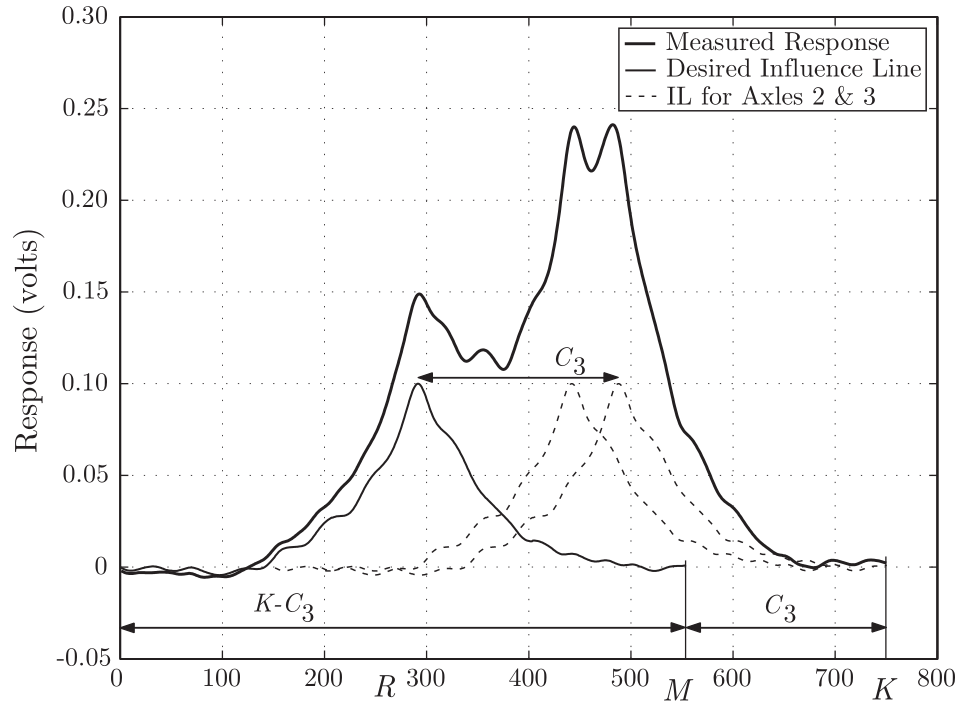
\includegraphics[width=\textwidth]{figures/strain_vs_influenceline}
	\caption{Placement of influence lines, influence line has been scaled.}
	\label{fig:strain_vs_influenceLine}
\end{figure}

When trying to place the influence line, it was found that axle detection needs to be very accurate for the calculation of axle loads. When using the method described above, with filtering to a degree where 8 peaks are found and to check how those peaks correspond with the known train's axle distances, proved to be accurate in some cases and very wrong in other cases. A wrongly found axle peak could for instance result in negative axle weights. A more general method which seems to place the influence better is to filter the signal to a degree where only the major peaks are found. It is believed that this peak is roughly the middle between closely spaced axles, or a bogie, on a train. Since the trains axles spacings are known, a successfully identified bogie location should place the influence line with a decent accuracy.
\begin{figure}[htbp]
	\centering
	% This file was created by matlab2tikz.
%
%The latest updates can be retrieved from
%  http://www.mathworks.com/matlabcentral/fileexchange/22022-matlab2tikz-matlab2tikz
%where you can also make suggestions and rate matlab2tikz.
%
\definecolor{mycolor1}{rgb}{0.00000,0.44700,0.74100}%
\definecolor{mycolor2}{rgb}{0.85000,0.32500,0.09800}%
\definecolor{mycolor3}{rgb}{1.00000,0.00000,1.00000}%
%
\begin{tikzpicture}

\begin{axis}[%
width=\textwidth,
height=0.4\textwidth,
at={(0\textwidth,0\textwidth)},
scale only axis,
xmin=0,
xmax=4000,
ymin=-5e-05,
ymax=0.0002,
axis background/.style={fill=white},
legend style={legend cell align=left,align=left,draw=white!15!black}
]
\addplot [color=mycolor1,solid]
  table[row sep=crcr]{%
1	3.76918588442974e-07\\
2	3.5304512042169e-07\\
3	3.29130219441135e-07\\
4	3.05187870958734e-07\\
5	2.81232144734613e-07\\
6	2.57277185761649e-07\\
7	2.33337205128069e-07\\
8	2.09426470817056e-07\\
9	1.85559298450098e-07\\
10	1.61750041979318e-07\\
11	1.38013084334367e-07\\
12	1.14362828030286e-07\\
13	9.08136857417148e-08\\
14	6.7380070849245e-08\\
15	4.40763879639611e-08\\
16	2.09170234358892e-08\\
17	-2.08366414811679e-09\\
18	-2.491135347037e-08\\
19	-4.75517699876649e-08\\
20	-6.99906954288706e-08\\
21	-9.2213977280144e-08\\
22	-1.14207538250951e-07\\
23	-1.35957385715924e-07\\
24	-1.57449621126509e-07\\
25	-1.78670449386874e-07\\
26	-1.99606188187877e-07\\
27	-2.2024327729468e-07\\
28	-2.40568287780625e-07\\
29	-2.60567931203853e-07\\
30	-2.80229068719412e-07\\
31	-2.99538720122396e-07\\
32	-3.18484072816599e-07\\
33	-3.3705249070258e-07\\
34	-3.55231522981338e-07\\
35	-3.7300891286638e-07\\
36	-3.90372606200969e-07\\
37	-4.07310759973908e-07\\
38	-4.23811750729522e-07\\
39	-4.39864182866988e-07\\
40	-4.55456896823287e-07\\
41	-4.70578977136127e-07\\
42	-4.85219760380916e-07\\
43	-4.99368842977604e-07\\
44	-5.13016088863021e-07\\
45	-5.2615163702351e-07\\
46	-5.38765908884177e-07\\
47	-5.5084961554961e-07\\
48	-5.62393764892452e-07\\
49	-5.73389668485111e-07\\
50	-5.83828948370911e-07\\
51	-5.93703543670082e-07\\
52	-6.03005717017765e-07\\
53	-6.11728060828813e-07\\
54	-6.1986350338661e-07\\
55	-6.27405314751968e-07\\
56	-6.34347112488663e-07\\
57	-6.40682867201964e-07\\
58	-6.46406907886935e-07\\
59	-6.51513927083405e-07\\
60	-6.55998985834257e-07\\
61	-6.59857518444056e-07\\
62	-6.63085337035226e-07\\
63	-6.65678635898567e-07\\
64	-6.67633995636085e-07\\
65	-6.68948387092871e-07\\
66	-6.69619175075595e-07\\
67	-6.69644121855589e-07\\
68	-6.69021390454083e-07\\
69	-6.67749547706952e-07\\
70	-6.65827567107815e-07\\
71	-6.63254831426466e-07\\
72	-6.60031135101558e-07\\
73	-6.56156686405564e-07\\
74	-6.51632109380192e-07\\
75	-6.4645844554075e-07\\
76	-6.40637155348528e-07\\
77	-6.34170119449069e-07\\
78	-6.2705963967577e-07\\
79	-6.19308439817274e-07\\
80	-6.10919666148299e-07\\
81	-6.01896887721988e-07\\
82	-5.9224409642391e-07\\
83	-5.81965706786777e-07\\
84	-5.71066555565198e-07\\
85	-5.59551901069783e-07\\
86	-5.47427422260946e-07\\
87	-5.34699217601323e-07\\
88	-5.21373803667401e-07\\
89	-5.07458113519618e-07\\
90	-4.92959494831719e-07\\
91	-4.77885707778537e-07\\
92	-4.6224492268398e-07\\
93	-4.46045717427431e-07\\
94	-4.29297074611593e-07\\
95	-4.12008378489802e-07\\
96	-3.94189411655427e-07\\
97	-3.75850351492903e-07\\
98	-3.57001766391855e-07\\
99	-3.37654611725014e-07\\
100	-3.17820225590939e-07\\
101	-2.97510324322855e-07\\
102	-2.7673699776447e-07\\
103	-2.55512704314732e-07\\
104	-2.33850265741915e-07\\
105	-2.11762861769749e-07\\
106	-1.89264024435892e-07\\
107	-1.6636763222571e-07\\
108	-1.43087903981818e-07\\
109	-1.19439392592179e-07\\
110	-9.54369784584092e-08\\
111	-7.10958627458837e-08\\
112	-4.64315604183264e-08\\
113	-2.1459893058676e-08\\
114	3.80301852152737e-09\\
115	2.93407618816161e-08\\
116	5.51366407582757e-08\\
117	8.11736830759676e-08\\
118	1.07434649159208e-07\\
119	1.33902040143826e-07\\
120	1.60558106584622e-07\\
121	1.87384857256635e-07\\
122	2.14364068147101e-07\\
123	2.41477291635649e-07\\
124	2.68705865858828e-07\\
125	2.96030924257056e-07\\
126	3.23433405299919e-07\\
127	3.50894062387348e-07\\
128	3.78393473922999e-07\\
129	4.05912053556853e-07\\
130	4.33430060593234e-07\\
131	4.60927610561557e-07\\
132	4.88384685945319e-07\\
133	5.15781147066842e-07\\
134	5.43096743123203e-07\\
135	5.70311123370681e-07\\
136	5.97403848452864e-07\\
137	6.24354401869888e-07\\
138	6.51142201583592e-07\\
139	6.77746611756155e-07\\
140	7.04146954617084e-07\\
141	7.30322522455363e-07\\
142	7.56252589731864e-07\\
143	7.81916425309218e-07\\
144	8.07293304793417e-07\\
145	8.32362522984283e-07\\
146	8.57103406429853e-07\\
147	8.81495326080467e-07\\
148	9.05517710038285e-07\\
149	9.29150056398062e-07\\
150	9.52371946174177e-07\\
151	9.75163056309843e-07\\
152	9.97503172764203e-07\\
153	1.01937220367177e-06\\
154	1.0407501925709e-06\\
155	1.06161733169527e-06\\
156	1.08195397532499e-06\\
157	1.10174065319129e-06\\
158	1.12095808393106e-06\\
159	1.13958718858559e-06\\
160	1.15760910413938e-06\\
161	1.17500519709335e-06\\
162	1.19175707706789e-06\\
163	1.20784661043113e-06\\
164	1.223255933946e-06\\
165	1.23796746843317e-06\\
166	1.25196393244248e-06\\
167	1.26522835592937e-06\\
168	1.27774409393026e-06\\
169	1.28949484023204e-06\\
170	1.30046464103002e-06\\
171	1.31063790856979e-06\\
172	1.31999943476647e-06\\
173	1.32853440479724e-06\\
174	1.33622841066099e-06\\
175	1.3430674646999e-06\\
176	1.34903801307727e-06\\
177	1.3541269492067e-06\\
178	1.35832162712614e-06\\
179	1.36160987481251e-06\\
180	1.36398000742977e-06\\
181	1.36542084050662e-06\\
182	1.36592170303655e-06\\
183	1.36547245049557e-06\\
184	1.36406347777176e-06\\
185	1.36168573200078e-06\\
186	1.35833072530165e-06\\
187	1.35399054740685e-06\\
188	1.34865787818204e-06\\
189	1.34232600002762e-06\\
190	1.33498881015855e-06\\
191	1.32664083275482e-06\\
192	1.31727723097776e-06\\
193	1.30689381884606e-06\\
194	1.29548707296559e-06\\
195	1.28305414410695e-06\\
196	1.26959286862535e-06\\
197	1.25510177971648e-06\\
198	1.23958011850263e-06\\
199	1.22302784494319e-06\\
200	1.20544564856349e-06\\
201	1.18683495899616e-06\\
202	1.16719795632907e-06\\
203	1.14653758125394e-06\\
204	1.12485754500927e-06\\
205	1.10216233911299e-06\\
206	1.07845724487676e-06\\
207	1.05374834269834e-06\\
208	1.0280425211243e-06\\
209	1.00134748567838e-06\\
210	9.73671767448892e-07\\
211	9.450247314296e-07\\
212	9.15416584608529e-07\\
213	8.84858383798181e-07\\
214	8.53362043201847e-07\\
215	8.20940341710539e-07\\
216	7.8760692992377e-07\\
217	7.53376336889739e-07\\
218	7.18263976557967e-07\\
219	6.82286153939995e-07\\
220	6.45460070971616e-07\\
221	6.07803832071067e-07\\
222	5.69336449388626e-07\\
223	5.30077847740644e-07\\
224	4.90048869224108e-07\\
225	4.49271277504985e-07\\
226	4.07767761776146e-07\\
227	3.65561940378673e-07\\
228	3.22678364082033e-07\\
229	2.79142519017314e-07\\
230	2.34980829259404e-07\\
231	1.90220659051748e-07\\
232	1.44890314669925e-07\\
233	9.90190459185028e-08\\
234	5.26370472566377e-08\\
235	5.77545854783538e-09\\
236	-4.15336345714926e-08\\
237	-8.92572007079688e-08\\
238	-1.37361263117566e-07\\
239	-1.85810900505216e-07\\
240	-2.34570248223421e-07\\
241	-2.8360249987253e-07\\
242	-3.32869909308176e-07\\
243	-3.82333793058631e-07\\
244	-4.31954533156592e-07\\
245	-4.81691580389101e-07\\
246	-5.31503457968421e-07\\
247	-5.81347765628676e-07\\
248	-6.3118118415026e-07\\
249	-6.80959480315957e-07\\
250	-7.30637512301973e-07\\
251	-7.80169235506102e-07\\
252	-8.29507708816578e-07\\
253	-8.78605101323817e-07\\
254	-9.27412699477845e-07\\
255	-9.75880914693185e-07\\
256	-1.02395929140458e-06\\
257	-1.07159651557401e-06\\
258	-1.11874042365229e-06\\
259	-1.1653380119961e-06\\
260	-1.21133544674249e-06\\
261	-1.25667807414154e-06\\
262	-1.30131043134947e-06\\
263	-1.34517625768198e-06\\
264	-1.38821850632964e-06\\
265	-1.43037935653546e-06\\
266	-1.47160022623491e-06\\
267	-1.51182178515956e-06\\
268	-1.55098396840312e-06\\
269	-1.5890259904508e-06\\
270	-1.62588635967124e-06\\
271	-1.66150289327029e-06\\
272	-1.69581273270632e-06\\
273	-1.72875235956572e-06\\
274	-1.76025761189756e-06\\
275	-1.79026370100616e-06\\
276	-1.8187052286996e-06\\
277	-1.84551620499277e-06\\
278	-1.87063006626246e-06\\
279	-1.89397969385286e-06\\
280	-1.91549743312789e-06\\
281	-1.93511511296881e-06\\
282	-1.95276406571349e-06\\
283	-1.96837514753398e-06\\
284	-1.98187875924945e-06\\
285	-1.99320486757043e-06\\
286	-2.00228302677071e-06\\
287	-2.00904240078219e-06\\
288	-2.01341178570923e-06\\
289	-2.01531963275669e-06\\
290	-2.01469407156779e-06\\
291	-2.01146293396599e-06\\
292	-2.00555377809575e-06\\
293	-1.99689391295643e-06\\
294	-1.98541042332372e-06\\
295	-1.97103019505202e-06\\
296	-1.9536799407518e-06\\
297	-1.93328622583481e-06\\
298	-1.90977549492086e-06\\
299	-1.88307409859887e-06\\
300	-1.85310832053406e-06\\
301	-1.81980440491505e-06\\
302	-1.78308858423142e-06\\
303	-1.742887107375e-06\\
304	-1.69912626805566e-06\\
305	-1.65173243352304e-06\\
306	-1.60063207358574e-06\\
307	-1.54575178991865e-06\\
308	-1.4870183456489e-06\\
309	-1.42435869521121e-06\\
310	-1.35770001446222e-06\\
311	-1.28696973104474e-06\\
312	-1.21209555499034e-06\\
313	-1.13300550955074e-06\\
314	-1.04962796224696e-06\\
315	-9.61891656124964e-07\\
316	-8.69725741206706e-07\\
317	-7.73059806126079e-07\\
318	-6.71823909935842e-07\\
319	-5.65948614076459e-07\\
320	-4.55365014492693e-07\\
321	-3.40004773886647e-07\\
322	-2.1980015409436e-07\\
323	-9.4684048573738e-08\\
324	3.54099850096412e-08\\
325	1.70547692111595e-07\\
326	3.10794088566108e-07\\
327	4.56213427784418e-07\\
328	6.06869167908561e-07\\
329	7.62823938934293e-07\\
330	9.24139509817062e-07\\
331	1.09087675557408e-06\\
332	1.26309562439897e-06\\
333	1.44085510480088e-06\\
334	1.62421319278446e-06\\
335	1.81322685908456e-06\\
336	2.0079520164705e-06\\
337	2.20844348713498e-06\\
338	2.41475497018295e-06\\
339	2.62693900923485e-06\\
340	2.84504696016021e-06\\
341	3.06912895895677e-06\\
342	3.29923388979038e-06\\
343	3.53540935321128e-06\\
344	3.77770163456267e-06\\
345	4.02615567259669e-06\\
346	4.28081502831407e-06\\
347	4.54172185404309e-06\\
348	4.80891686277326e-06\\
349	5.08243929776035e-06\\
350	5.36232690241804e-06\\
351	5.64861589051225e-06\\
352	5.94134091667442e-06\\
353	6.24053504724882e-06\\
354	6.54622973149129e-06\\
355	6.85845477313338e-06\\
356	7.17723830232964e-06\\
357	7.50260674800249e-06\\
358	7.83458481060141e-06\\
359	8.17319543529179e-06\\
360	8.51845978558904e-06\\
361	8.87039721745422e-06\\
362	9.22902525386569e-06\\
363	9.59435955988347e-06\\
364	9.96641391822076e-06\\
365	1.03452002053384e-05\\
366	1.07307283680769e-05\\
367	1.11230064008425e-05\\
368	1.15220403233594e-05\\
369	1.19278341590066e-05\\
370	1.23403899137506e-05\\
371	1.27597075556901e-05\\
372	1.31857849952277e-05\\
373	1.36186180658807e-05\\
374	1.40582005057459e-05\\
375	1.45045239396336e-05\\
376	1.49575778618813e-05\\
377	1.54173496198629e-05\\
378	1.58838243982061e-05\\
379	1.63569852037291e-05\\
380	1.68368128511118e-05\\
381	1.73232859493121e-05\\
382	1.78163808887395e-05\\
383	1.8316071829199e-05\\
384	1.88223306886158e-05\\
385	1.93351271325521e-05\\
386	1.98544285645275e-05\\
387	2.03802001171537e-05\\
388	2.0912404644093e-05\\
389	2.1451002712852e-05\\
390	2.19959525984187e-05\\
391	2.25472102777539e-05\\
392	2.31047294251451e-05\\
393	2.3668461408431e-05\\
394	2.42383552861069e-05\\
395	2.48143578053164e-05\\
396	2.53964134007397e-05\\
397	2.59844641943835e-05\\
398	2.65784499962803e-05\\
399	2.71783083061036e-05\\
400	2.77839743157053e-05\\
401	2.83953809125799e-05\\
402	2.90124586842614e-05\\
403	2.96351359236589e-05\\
404	3.02633386353319e-05\\
405	3.08969905427139e-05\\
406	3.15360130962834e-05\\
407	3.21803254826886e-05\\
408	3.28298446348264e-05\\
409	3.34844852428796e-05\\
410	3.4144159766312e-05\\
411	3.48087784468251e-05\\
412	3.54782493222748e-05\\
413	3.61524782415504e-05\\
414	3.68313688804149e-05\\
415	3.75148227583054e-05\\
416	3.82027392560945e-05\\
417	3.8895015634809e-05\\
418	3.9591547055305e-05\\
419	4.02922265988968e-05\\
420	4.09969452889371e-05\\
421	4.17055921133436e-05\\
422	4.2418054048069e-05\\
423	4.31342160815111e-05\\
424	4.38539612398555e-05\\
425	4.45771706133473e-05\\
426	4.5303723383486e-05\\
427	4.60334968511363e-05\\
428	4.67663664655476e-05\\
429	4.75022058542773e-05\\
430	4.8240886854006e-05\\
431	4.89822795422412e-05\\
432	4.97262522698951e-05\\
433	5.04726716947329e-05\\
434	5.12214028156771e-05\\
435	5.19723090079603e-05\\
436	5.27252520591149e-05\\
437	5.34800922057884e-05\\
438	5.42366881713729e-05\\
439	5.49948972044365e-05\\
440	5.57545751179439e-05\\
441	5.65155763292536e-05\\
442	5.72777539008774e-05\\
443	5.80409595819891e-05\\
444	5.88050438506678e-05\\
445	5.95698559568598e-05\\
446	6.03352439660464e-05\\
447	6.1101054803599e-05\\
448	6.18671342998072e-05\\
449	6.26333272355631e-05\\
450	6.33994773886843e-05\\
451	6.41654275808595e-05\\
452	6.49310197251969e-05\\
453	6.56960948743597e-05\\
454	6.64604932692685e-05\\
455	6.72240543883524e-05\\
456	6.79866169973302e-05\\
457	6.87480191995005e-05\\
458	6.95080984865227e-05\\
459	7.02666917896673e-05\\
460	7.10236355315158e-05\\
461	7.17787656780891e-05\\
462	7.25319177913828e-05\\
463	7.32829270822884e-05\\
464	7.40316284638791e-05\\
465	7.47778566050371e-05\\
466	7.55214459844013e-05\\
467	7.62622309446114e-05\\
468	7.70000457468277e-05\\
469	7.77347246255017e-05\\
470	7.84661018433756e-05\\
471	7.91940117466863e-05\\
472	7.99182888205511e-05\\
473	8.06387677445108e-05\\
474	8.1355283448207e-05\\
475	8.20676711671684e-05\\
476	8.27757664986826e-05\\
477	8.34794054577286e-05\\
478	8.41784245329469e-05\\
479	8.48726607426197e-05\\
480	8.55619516906396e-05\\
481	8.62461356224404e-05\\
482	8.69250514808651e-05\\
483	8.75985389619469e-05\\
484	8.82664385705777e-05\\
485	8.89285916760397e-05\\
486	8.95848405673747e-05\\
487	9.02350285085658e-05\\
488	9.08789997935079e-05\\
489	9.15165998007397e-05\\
490	9.21476750479155e-05\\
491	9.2772073245989e-05\\
492	9.33896433530858e-05\\
493	9.40002356280401e-05\\
494	9.46037016835701e-05\\
495	9.51998945390679e-05\\
496	9.57886686729811e-05\\
497	9.63698800747587e-05\\
498	9.69433862963403e-05\\
499	9.75090465031633e-05\\
500	9.80667215246638e-05\\
501	9.86162739042495e-05\\
502	9.91575679487195e-05\\
503	9.96904697771085e-05\\
504	0.000100214847368933\\
505	0.000100730570611815\\
506	0.000101237511348466\\
507	0.000101735543423001\\
508	0.000102224542726565\\
509	0.000102704387242258\\
510	0.000103174957089318\\
511	0.000103636134566564\\
512	0.000104087804195059\\
513	0.000104529852759987\\
514	0.000104962169351715\\
515	0.000105384645406024\\
516	0.000105797174743489\\
517	0.000106199653607994\\
518	0.000106591980704352\\
519	0.000106974057235026\\
520	0.000107345786935925\\
521	0.000107707076111257\\
522	0.00010805783366743\\
523	0.000108397971145976\\
524	0.000108727402755488\\
525	0.000109046045402554\\
526	0.00010935381872167\\
527	0.000109650645104121\\
528	0.000109936449725816\\
529	0.000110211160574061\\
530	0.000110474708473259\\
531	0.000110727027109529\\
532	0.000110968053054221\\
533	0.00011119772578633\\
534	0.000111415987713786\\
535	0.000111622784193614\\
536	0.000111818063550964\\
537	0.000112001777096984\\
538	0.000112173879145543\\
539	0.000112334327028785\\
540	0.000112483081111519\\
541	0.000112620104804424\\
542	0.000112745364576074\\
543	0.000112858829963778\\
544	0.000112960473583211\\
545	0.000113050271136864\\
546	0.000113128201421281\\
547	0.000113194246333092\\
548	0.000113248390873839\\
549	0.000113290623153593\\
550	0.000113320934393356\\
551	0.000113339318926256\\
552	0.000113345774197524\\
553	0.000113340300763263\\
554	0.000113322902288007\\
555	0.000113293585541067\\
556	0.000113252360391673\\
557	0.000113199239802913\\
558	0.000113134239824472\\
559	0.000113057379584168\\
560	0.000112968681278309\\
561	0.00011286817016085\\
562	0.000112755874531382\\
563	0.000112631825721941\\
564	0.000112496058082646\\
565	0.000112348608966191\\
566	0.000112189518711172\\
567	0.000112018830624282\\
568	0.000111836590961368\\
569	0.000111642848907367\\
570	0.000111437656555132\\
571	0.000111221068883151\\
572	0.000110993143732184\\
573	0.000110753941780818\\
574	0.000110503526519956\\
575	0.000110241964226258\\
576	0.000109969323934542\\
577	0.000109685677409165\\
578	0.000109391099114386\\
579	0.000109085666183748\\
580	0.000108769458388468\\
581	0.000108442558104879\\
582	0.000108105050280916\\
583	0.000107757022401676\\
584	0.000107398564454072\\
585	0.000107029768890592\\
586	0.000106650730592176\\
587	0.000106261546830251\\
588	0.000105862317227916\\
589	0.000105453143720321\\
590	0.000105034130514241\\
591	0.000104605384046879\\
592	0.000104167012943906\\
593	0.000103719127976774\\
594	0.000103261842019312\\
595	0.000102795270003626\\
596	0.000102319528875334\\
597	0.000101834737548152\\
598	0.000101341016857854\\
599	0.000100838489515628\\
600	0.000100327280060854\\
601	9.98075148133288e-05\\
602	9.92793218249507e-05\\
603	9.87428308309021e-05\\
604	9.81981732003435e-05\\
605	9.76454818866475e-05\\
606	9.70848913771959e-05\\
607	9.65165376427647e-05\\
608	9.59405580865209e-05\\
609	9.53570914926574e-05\\
610	9.47662779746878e-05\\
611	9.41682589234303e-05\\
612	9.35631769547011e-05\\
613	9.29511758567465e-05\\
614	9.23324005374348e-05\\
615	9.17069969712377e-05\\
616	9.1075112146022e-05\\
617	9.04368940096798e-05\\
618	8.97924914166211e-05\\
619	8.91420540741543e-05\\
620	8.84857324887799e-05\\
621	8.7823677912422e-05\\
622	8.71560422886236e-05\\
623	8.64829781987297e-05\\
624	8.58046388080837e-05\\
625	8.51211778122613e-05\\
626	8.44327493833682e-05\\
627	8.37395081164235e-05\\
628	8.30416089758557e-05\\
629	8.23392072421342e-05\\
630	8.16324584585609e-05\\
631	8.09215183782459e-05\\
632	8.02065429112901e-05\\
633	7.94876880721996e-05\\
634	7.87651099275545e-05\\
635	7.80389645439548e-05\\
636	7.73094079362669e-05\\
637	7.65765960161929e-05\\
638	7.5840684541185e-05\\
639	7.51018290637272e-05\\
640	7.43601848810055e-05\\
641	7.36159069849894e-05\\
642	7.2869150012943e-05\\
643	7.21200681983904e-05\\
644	7.13688153225519e-05\\
645	7.06155446662742e-05\\
646	6.98604089624718e-05\\
647	6.91035603491011e-05\\
648	6.83451503226852e-05\\
649	6.75853296924072e-05\\
650	6.68242485347921e-05\\
651	6.6062056148993e-05\\
652	6.52989010127012e-05\\
653	6.45349307386948e-05\\
654	6.3770292032044e-05\\
655	6.30051306479891e-05\\
656	6.22395913505054e-05\\
657	6.14738178715721e-05\\
658	6.07079528711588e-05\\
659	5.99421378979438e-05\\
660	5.91765133507786e-05\\
661	5.84112184409118e-05\\
662	5.76463911549842e-05\\
663	5.68821682188094e-05\\
664	5.61186850619497e-05\\
665	5.53560757831003e-05\\
666	5.45944731162912e-05\\
667	5.38340083979186e-05\\
668	5.30748115346143e-05\\
669	5.23170109719636e-05\\
670	5.15607336640792e-05\\
671	5.08061050440407e-05\\
672	5.00532489952068e-05\\
673	4.93022878234071e-05\\
674	4.85533422300213e-05\\
675	4.78065312859503e-05\\
676	4.70619724064874e-05\\
677	4.63197813270917e-05\\
678	4.55800720800704e-05\\
679	4.48429569721742e-05\\
680	4.41085465631075e-05\\
681	4.33769496449584e-05\\
682	4.26482732225504e-05\\
683	4.19226224947166e-05\\
684	4.12001008364999e-05\\
685	4.04808097822787e-05\\
686	3.97648490098191e-05\\
687	3.90523163252532e-05\\
688	3.83433076489833e-05\\
689	3.76379170025106e-05\\
690	3.69362364961868e-05\\
691	3.62383563178869e-05\\
692	3.55443647226003e-05\\
693	3.48543480229363e-05\\
694	3.41683905805428e-05\\
695	3.34865747984311e-05\\
696	3.28089811142049e-05\\
697	3.21356879941866e-05\\
698	3.1466771928437e-05\\
699	3.0802307426661e-05\\
700	3.01423670149945e-05\\
701	2.94870212336643e-05\\
702	2.88363386355145e-05\\
703	2.8190385785392e-05\\
704	2.75492272603822e-05\\
705	2.69129256508867e-05\\
706	2.62815415625349e-05\\
707	2.56551336189193e-05\\
708	2.50337584651448e-05\\
709	2.44174707721822e-05\\
710	2.38063232420161e-05\\
711	2.32003666135754e-05\\
712	2.25996496694355e-05\\
713	2.20042192432812e-05\\
714	2.14141202281184e-05\\
715	2.08293955852213e-05\\
716	2.02500863538052e-05\\
717	1.96762316614087e-05\\
718	1.91078687349754e-05\\
719	1.85450329126205e-05\\
720	1.79877576560679e-05\\
721	1.74360745637451e-05\\
722	1.68900133845222e-05\\
723	1.63496020320785e-05\\
724	1.58148665998846e-05\\
725	1.52858313767842e-05\\
726	1.47625188631596e-05\\
727	1.42449497876676e-05\\
728	1.37331431245293e-05\\
729	1.32271161113579e-05\\
730	1.27268842675102e-05\\
731	1.22324614129448e-05\\
732	1.17438596875707e-05\\
733	1.12610895710718e-05\\
734	1.07841599031894e-05\\
735	1.03130779044471e-05\\
736	9.84784919730217e-06\\
737	9.38847782770503e-06\\
738	8.93496628705303e-06\\
739	8.48731553451952e-06\\
740	8.04552501974246e-06\\
741	7.60959270585602e-06\\
742	7.17951509284809e-06\\
743	6.75528724122699e-06\\
744	6.33690279598072e-06\\
745	5.92435401081188e-06\\
746	5.51763177263153e-06\\
747	5.11672562629572e-06\\
748	4.72162379956695e-06\\
749	4.3323132282853e-06\\
750	3.94877958173136e-06\\
751	3.57100728816601e-06\\
752	3.19897956052873e-06\\
753	2.83267842227982e-06\\
754	2.4720847333696e-06\\
755	2.1171782163185e-06\\
756	1.7679374823919e-06\\
757	1.42434005785467e-06\\
758	1.08636241028846e-06\\
759	7.53979974957499e-07\\
760	4.27167181206624e-07\\
761	1.0589747887654e-07\\
762	-2.09856635278691e-07\\
763	-5.20123591186498e-07\\
764	-8.24932719078307e-07\\
765	-1.12431422315368e-06\\
766	-1.4182991553005e-06\\
767	-1.7069193888851e-06\\
768	-1.99020759262665e-06\\
769	-2.26819720456865e-06\\
770	-2.54092240616139e-06\\
771	-2.80841809646858e-06\\
772	-3.07071986651055e-06\\
773	-3.32786397375696e-06\\
774	-3.57988731678132e-06\\
775	-3.82682741008926e-06\\
776	-4.06872235913228e-06\\
777	-4.30561083551932e-06\\
778	-4.53753205243578e-06\\
779	-4.76452574028232e-06\\
780	-4.98663212254385e-06\\
781	-5.20389189189861e-06\\
782	-5.41634618657734e-06\\
783	-5.62403656698311e-06\\
784	-5.82700499258034e-06\\
785	-6.02529379906259e-06\\
786	-6.21894567580788e-06\\
787	-6.40800364362986e-06\\
788	-6.59251103283318e-06\\
789	-6.77251146158084e-06\\
790	-6.94804881458103e-06\\
791	-7.11916722210052e-06\\
792	-7.28591103931185e-06\\
793	-7.44832482598029e-06\\
794	-7.60645332649737e-06\\
795	-7.76034145026635e-06\\
796	-7.91003425244552e-06\\
797	-8.05557691505423e-06\\
798	-8.19701472844686e-06\\
799	-8.33439307315903e-06\\
800	-8.46775740213041e-06\\
801	-8.59715322330785e-06\\
802	-8.7226260826326e-06\\
803	-8.84422154741454e-06\\
804	-8.96198519009687e-06\\
805	-9.07596257241314e-06\\
806	-9.18619922993931e-06\\
807	-9.29274065704278e-06\\
808	-9.39563229222996e-06\\
809	-9.49491950389336e-06\\
810	-9.59064757645989e-06\\
811	-9.68286169694013e-06\\
812	-9.77160694187984e-06\\
813	-9.85692826471334e-06\\
814	-9.93887048351841e-06\\
815	-1.00174782691726e-05\\
816	-1.00927961339094e-05\\
817	-1.01648684202747e-05\\
818	-1.02337392904799e-05\\
819	-1.02994527161522e-05\\
820	-1.03620524684786e-05\\
821	-1.04215821087426e-05\\
822	-1.04780849792498e-05\\
823	-1.05316041946415e-05\\
824	-1.05821826335907e-05\\
825	-1.06298629308806e-05\\
826	-1.06746874698592e-05\\
827	-1.07166983752681e-05\\
828	-1.07559375064402e-05\\
829	-1.07924464508645e-05\\
830	-1.082626651811e-05\\
831	-1.08574387341084e-05\\
832	-1.08860038357869e-05\\
833	-1.09120022660485e-05\\
834	-1.09354741690947e-05\\
835	-1.09564593860834e-05\\
836	-1.09749974511181e-05\\
837	-1.09911275875629e-05\\
838	-1.10048887046756e-05\\
839	-1.10163193945553e-05\\
840	-1.10254579293957e-05\\
841	-1.10323422590408e-05\\
842	-1.10370100088336e-05\\
843	-1.10394984777534e-05\\
844	-1.10398446368336e-05\\
845	-1.10380851278545e-05\\
846	-1.10342562623024e-05\\
847	-1.102839402059e-05\\
848	-1.10205340515297e-05\\
849	-1.10107116720523e-05\\
850	-1.09989618671658e-05\\
851	-1.09853192901436e-05\\
852	-1.09698182629389e-05\\
853	-1.09524927768137e-05\\
854	-1.09333764931779e-05\\
855	-1.09125027446292e-05\\
856	-1.0889904536187e-05\\
857	-1.08656145467128e-05\\
858	-1.0839665130508e-05\\
859	-1.08120883190838e-05\\
860	-1.07829158230937e-05\\
861	-1.07521790344206e-05\\
862	-1.07199090284135e-05\\
863	-1.06861365662625e-05\\
864	-1.06508920975069e-05\\
865	-1.06142057626684e-05\\
866	-1.05761073960012e-05\\
867	-1.05366265283512e-05\\
868	-1.04957923901182e-05\\
869	-1.04536339143121e-05\\
870	-1.04101797396962e-05\\
871	-1.03654582140109e-05\\
872	-1.03194973972689e-05\\
873	-1.02723250651167e-05\\
874	-1.02239687122533e-05\\
875	-1.01744555559005e-05\\
876	-1.0123812539317e-05\\
877	-1.00720663353493e-05\\
878	-1.00192433500135e-05\\
879	-9.96536972610025e-06\\
880	-9.91047134679646e-06\\
881	-9.85457383931828e-06\\
882	-9.79770257854708e-06\\
883	-9.73988269066412e-06\\
884	-9.68113905677655e-06\\
885	-9.62149631652893e-06\\
886	-9.56097887169466e-06\\
887	-9.49961088974138e-06\\
888	-9.43741630736441e-06\\
889	-9.3744188339836e-06\\
890	-9.31064195519712e-06\\
891	-9.24610893618793e-06\\
892	-9.18084282507696e-06\\
893	-9.11486645621932e-06\\
894	-9.04820245343751e-06\\
895	-8.98087323318759e-06\\
896	-8.91290100765406e-06\\
897	-8.84430778776871e-06\\
898	-8.77511538614962e-06\\
899	-8.70534541995614e-06\\
900	-8.635019313656e-06\\
901	-8.56415830170129e-06\\
902	-8.49278343110909e-06\\
903	-8.42091556394415e-06\\
904	-8.34857537970005e-06\\
905	-8.27578337757568e-06\\
906	-8.20255987864507e-06\\
907	-8.12892502791637e-06\\
908	-8.05489879627918e-06\\
909	-7.98050098233657e-06\\
910	-7.90575121412036e-06\\
911	-7.83066895068728e-06\\
912	-7.75527348359431e-06\\
913	-7.67958393825156e-06\\
914	-7.60361927515093e-06\\
915	-7.52739829096947e-06\\
916	-7.45093961954606e-06\\
917	-7.37426173273044e-06\\
918	-7.29738294110356e-06\\
919	-7.22032139456875e-06\\
920	-7.14309508281297e-06\\
921	-7.06572183563774e-06\\
922	-6.98821932315942e-06\\
923	-6.91060505587877e-06\\
924	-6.83289638462008e-06\\
925	-6.75511050033917e-06\\
926	-6.67726443380177e-06\\
927	-6.59937505513166e-06\\
928	-6.52145907322981e-06\\
929	-6.44353303506474e-06\\
930	-6.36561332483546e-06\\
931	-6.28771616300757e-06\\
932	-6.20985760522355e-06\\
933	-6.13205354108907e-06\\
934	-6.05431969283563e-06\\
935	-5.97667161386201e-06\\
936	-5.89912468715545e-06\\
937	-5.82169412359428e-06\\
938	-5.74439496013425e-06\\
939	-5.66724205787968e-06\\
940	-5.59025010004213e-06\\
941	-5.5134335897881e-06\\
942	-5.43680684797829e-06\\
943	-5.36038401080056e-06\\
944	-5.28417902729887e-06\\
945	-5.20820565680035e-06\\
946	-5.13247746624383e-06\\
947	-5.05700782741151e-06\\
948	-4.98180991406668e-06\\
949	-4.90689669900056e-06\\
950	-4.83228095099029e-06\\
951	-4.75797523167175e-06\\
952	-4.68399189232936e-06\\
953	-4.61034307060636e-06\\
954	-4.5370406871378e-06\\
955	-4.46409644211032e-06\\
956	-4.39152181175079e-06\\
957	-4.31932804474744e-06\\
958	-4.2475261586065e-06\\
959	-4.17612693594746e-06\\
960	-4.10514092074018e-06\\
961	-4.03457841448705e-06\\
962	-3.96444947235352e-06\\
963	-3.89476389924999e-06\\
964	-3.82553124586853e-06\\
965	-3.75676080467781e-06\\
966	-3.68846160587922e-06\\
967	-3.62064241332742e-06\\
968	-3.55331172041926e-06\\
969	-3.48647774595327e-06\\
970	-3.42014842996392e-06\\
971	-3.3543314295335e-06\\
972	-3.2890341145848e-06\\
973	-3.2242635636581e-06\\
974	-3.16002655967519e-06\\
975	-3.09632958569447e-06\\
976	-3.03317882065924e-06\\
977	-2.97058013514311e-06\\
978	-2.90853908709545e-06\\
979	-2.84706091758965e-06\\
980	-2.78615054657768e-06\\
981	-2.72581256865379e-06\\
982	-2.66605124883033e-06\\
983	-2.60687051832854e-06\\
984	-2.54827397038739e-06\\
985	-2.49026485609338e-06\\
986	-2.4328460802337e-06\\
987	-2.37602019717624e-06\\
988	-2.31978940677842e-06\\
989	-2.26415555032826e-06\\
990	-2.20912010651954e-06\\
991	-2.1546841874644e-06\\
992	-2.10084853474541e-06\\
993	-2.04761351550985e-06\\
994	-1.99497911860847e-06\\
995	-1.94294495078148e-06\\
996	-1.8915102328931e-06\\
997	-1.84067379621862e-06\\
998	-1.79043407878466e-06\\
999	-1.74078912176528e-06\\
1000	-1.69173656593667e-06\\
1001	-1.64327364819145e-06\\
1002	-1.59539719811549e-06\\
1003	-1.54810363462851e-06\\
1004	-1.5013889626908e-06\\
1005	-1.45524877007794e-06\\
1006	-1.40967822422466e-06\\
1007	-1.36467206914069e-06\\
1008	-1.32022462239905e-06\\
1009	-1.27632977219944e-06\\
1010	-1.23298097450774e-06\\
1011	-1.19017125027325e-06\\
1012	-1.14789318272536e-06\\
1013	-1.10613891475076e-06\\
1014	-1.06490014635292e-06\\
1015	-1.02416813219499e-06\\
1016	-9.83933679227492e-07\\
1017	-9.44187144401808e-07\\
1018	-9.04918432471197e-07\\
1019	-8.66116993880122e-07\\
1020	-8.27771822743057e-07\\
1021	-7.89871454914007e-07\\
1022	-7.52403966147804e-07\\
1023	-7.15356970353855e-07\\
1024	-6.78717617944201e-07\\
1025	-6.42472594275592e-07\\
1026	-6.06608118187878e-07\\
1027	-5.71109940638384e-07\\
1028	-5.35963343434204e-07\\
1029	-5.01153138062489e-07\\
1030	-4.66663664620241e-07\\
1031	-4.3247879084353e-07\\
1032	-3.98581911238274e-07\\
1033	-3.64955946311871e-07\\
1034	-3.3158334190764e-07\\
1035	-2.9844606864222e-07\\
1036	-2.655256214471e-07\\
1037	-2.32803019214342e-07\\
1038	-2.00258804548112e-07\\
1039	-1.67873043622181e-07\\
1040	-1.35625326144236e-07\\
1041	-1.03494765428017e-07\\
1042	-7.14599985734308e-08\\
1043	-3.94991867563621e-08\\
1044	-7.59001562778567e-09\\
1045	2.42903041762876e-08\\
1046	5.61650364132777e-08\\
1047	8.80579185005637e-08\\
1048	1.19993160668766e-07\\
1049	1.51995445001574e-07\\
1050	1.84089924360462e-07\\
1051	2.16302221194344e-07\\
1052	2.48658426232469e-07\\
1053	2.81185097060226e-07\\
1054	3.13909256576958e-07\\
1055	3.46858391334145e-07\\
1056	3.80060449753728e-07\\
1057	4.13543840225596e-07\\
1058	4.47337429082454e-07\\
1059	4.81470538451536e-07\\
1060	5.15972943982487e-07\\
1061	5.50874872449416e-07\\
1062	5.86206999226202e-07\\
1063	6.22000445634699e-07\\
1064	6.58286776163297e-07\\
1065	6.95097995555489e-07\\
1066	7.32466545766977e-07\\
1067	7.70425302789819e-07\\
1068	8.09007573342226e-07\\
1069	8.48247091422968e-07\\
1070	8.88178014728308e-07\\
1071	9.28834920930793e-07\\
1072	9.70252803817594e-07\\
1073	1.01246706928755e-06\\
1074	1.05551353120451e-06\\
1075	1.09942840710635e-06\\
1076	1.14424831376715e-06\\
1077	1.19001026261117e-06\\
1078	1.23675165497704e-06\\
1079	1.28451027723004e-06\\
1080	1.33332429572102e-06\\
1081	1.38323225159014e-06\\
1082	1.43427305541289e-06\\
1083	1.48648598168763e-06\\
1084	1.53991066316182e-06\\
1085	1.59458708499545e-06\\
1086	1.65055557875925e-06\\
1087	1.70785681626658e-06\\
1088	1.76653180323611e-06\\
1089	1.82662187278333e-06\\
1090	1.88816867873953e-06\\
1091	1.95121418879571e-06\\
1092	2.01580067746896e-06\\
1093	2.08197071889028e-06\\
1094	2.14976717941056e-06\\
1095	2.21923321002382e-06\\
1096	2.29041223860431e-06\\
1097	2.3633479619566e-06\\
1098	2.4380843376758e-06\\
1099	2.51466557581619e-06\\
1100	2.59313613036588e-06\\
1101	2.67354069052578e-06\\
1102	2.75592417179063e-06\\
1103	2.84033170683001e-06\\
1104	2.92680863616779e-06\\
1105	3.01540049865708e-06\\
1106	3.10615302175e-06\\
1107	3.19911211155921e-06\\
1108	3.29432384271014e-06\\
1109	3.39183444798171e-06\\
1110	3.4916903077337e-06\\
1111	3.59393793911922e-06\\
1112	3.69862398508098e-06\\
1113	3.8057952031284e-06\\
1114	3.91549845389581e-06\\
1115	4.02778068947899e-06\\
1116	4.14268894154887e-06\\
1117	4.26027030924159e-06\\
1118	4.38057194682261e-06\\
1119	4.50364105112496e-06\\
1120	4.62952484875954e-06\\
1121	4.75827058309693e-06\\
1122	4.88992550101972e-06\\
1123	5.02453683944443e-06\\
1124	5.16215181161261e-06\\
1125	5.30281759315033e-06\\
1126	5.44658130789553e-06\\
1127	5.59349001349305e-06\\
1128	5.74359068675703e-06\\
1129	5.8969302088008e-06\\
1130	6.05355534993351e-06\\
1131	6.21351275432512e-06\\
1132	6.37684892443843e-06\\
1133	6.54361020522988e-06\\
1134	6.71384276811884e-06\\
1135	6.88759259472701e-06\\
1136	7.06490546038807e-06\\
1137	7.24582691742892e-06\\
1138	7.43040227822407e-06\\
1139	7.61867659802436e-06\\
1140	7.81069465756153e-06\\
1141	8.00650094543021e-06\\
1142	8.20613964025019e-06\\
1143	8.40965459261001e-06\\
1144	8.61708930679491e-06\\
1145	8.82848692230132e-06\\
1146	9.04389019514084e-06\\
1147	9.26334147893648e-06\\
1148	9.48688270581451e-06\\
1149	9.71455536709474e-06\\
1150	9.94640049378325e-06\\
1151	1.01824586368714e-05\\
1152	1.04227698474444e-05\\
1153	1.06673736566045e-05\\
1154	1.09163090552126e-05\\
1155	1.1169614473453e-05\\
1156	1.1427327760226e-05\\
1157	1.16894861623742e-05\\
1158	1.19561263037467e-05\\
1159	1.22272841641072e-05\\
1160	1.25029950578922e-05\\
1161	1.27832936128243e-05\\
1162	1.30682137483877e-05\\
1163	1.33577886541719e-05\\
1164	1.36520507680904e-05\\
1165	1.39510317544811e-05\\
1166	1.42547624820957e-05\\
1167	1.45632730019865e-05\\
1168	1.48765925252949e-05\\
1169	1.51947494009544e-05\\
1170	1.55177710933115e-05\\
1171	1.58456841596764e-05\\
1172	1.61785142278086e-05\\
1173	1.65162859733502e-05\\
1174	1.68590230972119e-05\\
1175	1.72067483029235e-05\\
1176	1.75594832739581e-05\\
1177	1.79172486510381e-05\\
1178	1.82800640094346e-05\\
1179	1.86479478362701e-05\\
1180	1.90209175078333e-05\\
1181	1.93989892669184e-05\\
1182	1.9782178200199e-05\\
1183	2.01704982156471e-05\\
1184	2.05639620200089e-05\\
1185	2.09625810963484e-05\\
1186	2.13663656816711e-05\\
1187	2.17753247446381e-05\\
1188	2.21894659633844e-05\\
1189	2.26087957034518e-05\\
1190	2.30333189958501e-05\\
1191	2.34630395152577e-05\\
1192	2.38979595583757e-05\\
1193	2.43380800224468e-05\\
1194	2.47834003839539e-05\\
1195	2.52339186775085e-05\\
1196	2.5689631474946e-05\\
1197	2.61505338646375e-05\\
1198	2.66166194310346e-05\\
1199	2.70878802344591e-05\\
1200	2.75643067911515e-05\\
1201	2.80458880535937e-05\\
1202	2.85326113911172e-05\\
1203	2.90244625708136e-05\\
1204	2.95214257387597e-05\\
1205	3.00234834015723e-05\\
1206	3.05306164083064e-05\\
1207	3.10428039327123e-05\\
1208	3.15600234558643e-05\\
1209	3.20822507491774e-05\\
1210	3.26094598578244e-05\\
1211	3.31416230845704e-05\\
1212	3.36787109740365e-05\\
1213	3.42206922974101e-05\\
1214	3.4767534037614e-05\\
1215	3.53192013749496e-05\\
1216	3.58756576732304e-05\\
1217	3.6436864466417e-05\\
1218	3.70027814457713e-05\\
1219	3.75733664475425e-05\\
1220	3.81485754411994e-05\\
1221	3.87283625182244e-05\\
1222	3.93126798814818e-05\\
1223	3.99014778351762e-05\\
1224	4.04947047754136e-05\\
1225	4.10923071813801e-05\\
1226	4.16942296071514e-05\\
1227	4.23004146741477e-05\\
1228	4.29108030642457e-05\\
1229	4.35253335135636e-05\\
1230	4.41439428069299e-05\\
1231	4.47665657730508e-05\\
1232	4.53931352803883e-05\\
1233	4.60235822337612e-05\\
1234	4.66578355716833e-05\\
1235	4.72958222644482e-05\\
1236	4.79374673129757e-05\\
1237	4.85826937484292e-05\\
1238	4.92314226326176e-05\\
1239	4.98835730591911e-05\\
1240	5.05390621556436e-05\\
1241	5.11978050861309e-05\\
1242	5.18597150551168e-05\\
1243	5.25247033118556e-05\\
1244	5.31926791557223e-05\\
1245	5.38635499423984e-05\\
1246	5.45372210909242e-05\\
1247	5.52135960916253e-05\\
1248	5.58925765149222e-05\\
1249	5.65740620210306e-05\\
1250	5.72579503705614e-05\\
1251	5.79441374360262e-05\\
1252	5.86325172142565e-05\\
1253	5.93229818397427e-05\\
1254	6.0015421598899e-05\\
1255	6.070972494526e-05\\
1256	6.14057785156147e-05\\
1257	6.21034671470828e-05\\
1258	6.28026738951365e-05\\
1259	6.3503280052574e-05\\
1260	6.42051651694462e-05\\
1261	6.49082070739415e-05\\
1262	6.56122818942295e-05\\
1263	6.63172640812669e-05\\
1264	6.70230264325676e-05\\
1265	6.77294401169367e-05\\
1266	6.84363747001708e-05\\
1267	6.9143698171723e-05\\
1268	6.98512769723337e-05\\
1269	7.0558976022626e-05\\
1270	7.12666587526632e-05\\
1271	7.19741871324684e-05\\
1272	7.26814217035015e-05\\
1273	7.33882216110932e-05\\
1274	7.40944446378299e-05\\
1275	7.47999472378871e-05\\
1276	7.55045845723058e-05\\
1277	7.6208210545208e-05\\
1278	7.69106778409433e-05\\
1279	7.76118379621628e-05\\
1280	7.83115412688114e-05\\
1281	7.90096370180329e-05\\
1282	7.97059734049781e-05\\
1283	8.0400397604509e-05\\
1284	8.10927558137888e-05\\
1285	8.17828932957483e-05\\
1286	8.24706544234196e-05\\
1287	8.31558827251243e-05\\
1288	8.38384209305062e-05\\
1289	8.45181110173968e-05\\
1290	8.51947942594993e-05\\
1291	8.5868311274881e-05\\
1292	8.65385020752569e-05\\
1293	8.72052061160539e-05\\
1294	8.78682623472377e-05\\
1295	8.85275092648898e-05\\
1296	8.91827849635169e-05\\
1297	8.9833927189077e-05\\
1298	9.04807733927057e-05\\
1299	9.11231607851242e-05\\
1300	9.17609263917126e-05\\
1301	9.2393907108228e-05\\
1302	9.30219397571506e-05\\
1303	9.36448611446359e-05\\
1304	9.42625081180555e-05\\
1305	9.48747176241037e-05\\
1306	9.54813267674504e-05\\
1307	9.6082172869918e-05\\
1308	9.66770935301604e-05\\
1309	9.72659266838229e-05\\
1310	9.78485106641572e-05\\
1311	9.84246842630718e-05\\
1312	9.89942867925909e-05\\
1313	9.95571581466995e-05\\
1314	0.000100113138863549\\
1315	0.000100662070187999\\
1316	0.000101203794134469\\
1317	0.000101738153550076\\
1318	0.000102264992178028\\
1319	0.000102784154721251\\
1320	0.00010329548690622\\
1321	0.000103798835546969\\
1322	0.00010429404860925\\
1323	0.00010478097527481\\
1324	0.00010525946600577\\
1325	0.000105729372609063\\
1326	0.000106190548300909\\
1327	0.000106642847771299\\
1328	0.000107086127248458\\
1329	0.000107520244563251\\
1330	0.000107945059213518\\
1331	0.000108360432428285\\
1332	0.000108766227231845\\
1333	0.000109162308507661\\
1334	0.000109548543062066\\
1335	0.000109924799687739\\
1336	0.000110290949226906\\
1337	0.000110646864634254\\
1338	0.000110992421039516\\
1339	0.000111327495809706\\
1340	0.000111651968610958\\
1341	0.000111965721469952\\
1342	0.000112268638834891\\
1343	0.000112560607635992\\
1344	0.000112841517345473\\
1345	0.000113111260036989\\
1346	0.000113369730444499\\
1347	0.000113616826020527\\
1348	0.000113852446993786\\
1349	0.000114076496426136\\
1350	0.000114288880268844\\
1351	0.000114489507418113\\
1352	0.000114678289769862\\
1353	0.000114855142273703\\
1354	0.000115019982986113\\
1355	0.000115172733122745\\
1356	0.000115313317109869\\
1357	0.0001154416626349\\
1358	0.000115557700695993\\
1359	0.000115661365650667\\
1360	0.00011575259526344\\
1361	0.000115831330752433\\
1362	0.000115897516834931\\
1363	0.000115951101771862\\
1364	0.000115992037411167\\
1365	0.00011602027923004\\
1366	0.000116035786376013\\
1367	0.000116038521706844\\
1368	0.000116028451829202\\
1369	0.000116005547136115\\
1370	0.000115969781843154\\
1371	0.00011592113402333\\
1372	0.000115859585640688\\
1373	0.000115785122582556\\
1374	0.000115697734690453\\
1375	0.000115597415789603\\
1376	0.000115484163717066\\
1377	0.00011535798034843\\
1378	0.000115218871623077\\
1379	0.000115066847567975\\
1380	0.000114901922319999\\
1381	0.000114724114146741\\
1382	0.000114533445465814\\
1383	0.000114329942862609\\
1384	0.000114113637106505\\
1385	0.000113884563165512\\
1386	0.000113642760219323\\
1387	0.000113388271670775\\
1388	0.000113121145155687\\
1389	0.000112841432551081\\
1390	0.000112549189981756\\
1391	0.000112244477825216\\
1392	0.000111927360714929\\
1393	0.000111597907541918\\
1394	0.000111256191454671\\
1395	0.000110902289857349\\
1396	0.000110536284406306\\
1397	0.000110158261004892\\
1398	0.000109768309796551\\
1399	0.00010936652515619\\
1400	0.000108953005679829\\
1401	0.000108527854172521\\
1402	0.000108091177634538\\
1403	0.000107643087245826\\
1404	0.000107183698348718\\
1405	0.000106713130428911\\
1406	0.000106231507094712\\
1407	0.000105738956054537\\
1408	0.000105235609092681\\
1409	0.000104721602043357\\
1410	0.000104197074762999\\
1411	0.000103662171100845\\
1412	0.000103117038867799\\
1413	0.000102561829803577\\
1414	0.000101996699542148\\
1415	0.000101421807575471\\
1416	0.000100837317215544\\
1417	0.000100243395554767\\
1418	9.96402134246379e-05\\
1419	9.90279453527785e-05\\
1420	9.84067695183185e-05\\
1421	9.77768677056378e-05\\
1422	9.71384252564861e-05\\
1423	9.64916310204922e-05\\
1424	9.58366773040794e-05\\
1425	9.51737598178008e-05\\
1426	9.45030776221136e-05\\
1427	9.38248330716071e-05\\
1428	9.31392317577052e-05\\
1429	9.24464824498611e-05\\
1430	9.1746797035263e-05\\
1431	9.10403904570739e-05\\
1432	9.03274806512248e-05\\
1433	8.96082884817837e-05\\
1434	8.88830376749238e-05\\
1435	8.81519547515136e-05\\
1436	8.74152689583546e-05\\
1437	8.6673212198089e-05\\
1438	8.59260189578065e-05\\
1439	8.51739262363728e-05\\
1440	8.44171734705104e-05\\
1441	8.36560024596564e-05\\
1442	8.2890657289627e-05\\
1443	8.21213842551189e-05\\
1444	8.13484317810738e-05\\
1445	8.05720503429399e-05\\
1446	7.97924923858586e-05\\
1447	7.90100122428091e-05\\
1448	7.82248660517421e-05\\
1449	7.74373116717355e-05\\
1450	7.66476085982052e-05\\
1451	7.58560178772041e-05\\
1452	7.50628020188435e-05\\
1453	7.42682249098711e-05\\
1454	7.34725517254424e-05\\
1455	7.26760488401169e-05\\
1456	7.18789837381202e-05\\
1457	7.10816249229038e-05\\
1458	7.02842418260412e-05\\
1459	6.94871047154984e-05\\
1460	6.86904846033131e-05\\
1461	6.78946531527239e-05\\
1462	6.70998825847849e-05\\
1463	6.63064455845056e-05\\
1464	6.55146152065536e-05\\
1465	6.47246647805601e-05\\
1466	6.39368678160672e-05\\
1467	6.3151497907155e-05\\
1468	6.23688286367901e-05\\
1469	6.15891334809342e-05\\
1470	6.08126857124526e-05\\
1471	6.00397583048632e-05\\
1472	5.92706238359658e-05\\
1473	5.85055543913925e-05\\
1474	5.77448214681191e-05\\
1475	5.69886958779784e-05\\
1476	5.62374476512151e-05\\
1477	5.54913459401245e-05\\
1478	5.47506589228135e-05\\
1479	5.40156537071257e-05\\
1480	5.32865962347713e-05\\
1481	5.25637511857005e-05\\
1482	5.18473818827634e-05\\
1483	5.11377501966941e-05\\
1484	5.04351164514607e-05\\
1485	4.97397393300204e-05\\
1486	4.90518757805207e-05\\
1487	4.8371780922984e-05\\
1488	4.76997079565179e-05\\
1489	4.70359080670883e-05\\
1490	4.63806303358954e-05\\
1491	4.57341216483909e-05\\
1492	4.50966266039747e-05\\
1493	4.44683874264097e-05\\
1494	4.38496438749925e-05\\
1495	4.32406331565171e-05\\
1496	4.26415898380689e-05\\
1497	4.20527457606861e-05\\
1498	4.14743299539244e-05\\
1499	4.09065685513618e-05\\
1500	4.03496847070776e-05\\
1501	3.98038985131424e-05\\
1502	3.92694269181525e-05\\
1503	3.87464836468434e-05\\
1504	3.82352791208165e-05\\
1505	3.77360203804106e-05\\
1506	3.72489110077533e-05\\
1507	3.67741510510216e-05\\
1508	3.6311936949946e-05\\
1509	3.58624614625866e-05\\
1510	3.54259135934138e-05\\
1511	3.50024785227212e-05\\
1512	3.45923375374017e-05\\
1513	3.41956679631147e-05\\
1514	3.38126430978715e-05\\
1515	3.34434321470675e-05\\
1516	3.30882001599869e-05\\
1517	3.27471079678055e-05\\
1518	3.24203121231186e-05\\
1519	3.21079648410155e-05\\
1520	3.18102139417274e-05\\
1521	3.15272027948696e-05\\
1522	3.12590702653016e-05\\
1523	3.10059506606259e-05\\
1524	3.07679736803468e-05\\
1525	3.05452643667088e-05\\
1526	3.03379430572349e-05\\
1527	3.01461253389809e-05\\
1528	2.99699220045272e-05\\
1529	2.98094390097211e-05\\
1530	2.96647774331882e-05\\
1531	2.95360334376278e-05\\
1532	2.94232982329058e-05\\
1533	2.93266580409597e-05\\
1534	2.92461940625287e-05\\
1535	2.91819824457198e-05\\
1536	2.91340942564222e-05\\
1537	2.91025954505803e-05\\
1538	2.90875468483338e-05\\
1539	2.90890041100345e-05\\
1540	2.91070177141478e-05\\
1541	2.91416329370448e-05\\
1542	2.91928898346918e-05\\
1543	2.92608232262434e-05\\
1544	2.93454626795417e-05\\
1545	2.94468324985264e-05\\
1546	2.95649517125591e-05\\
1547	2.96998340676618e-05\\
1548	2.98514880196726e-05\\
1549	3.00199167293181e-05\\
1550	3.02051180592013e-05\\
1551	3.04070845727042e-05\\
1552	3.06258035348028e-05\\
1553	3.08612569147914e-05\\
1554	3.1113421390911e-05\\
1555	3.13822683568799e-05\\
1556	3.16677639303172e-05\\
1557	3.19698689630558e-05\\
1558	3.22885390533365e-05\\
1559	3.26237245598748e-05\\
1560	3.29753706177922e-05\\
1561	3.33434171564031e-05\\
1562	3.37277989188445e-05\\
1563	3.41284454835406e-05\\
1564	3.4545281287488e-05\\
1565	3.49782256513495e-05\\
1566	3.54271928063436e-05\\
1567	3.58920919229151e-05\\
1568	3.63728271411724e-05\\
1569	3.68692976030746e-05\\
1570	3.73813974863544e-05\\
1571	3.79090160401575e-05\\
1572	3.84520376223826e-05\\
1573	3.90103417387026e-05\\
1574	3.95838030832484e-05\\
1575	4.01722915809355e-05\\
1576	4.0775672431414e-05\\
1577	4.13938061546193e-05\\
1578	4.20265486379037e-05\\
1579	4.26737511847261e-05\\
1580	4.33352605648772e-05\\
1581	4.40109190662164e-05\\
1582	4.47005645478976e-05\\
1583	4.54040304950587e-05\\
1584	4.61211460749502e-05\\
1585	4.68517361944778e-05\\
1586	4.75956215591321e-05\\
1587	4.835261873328e-05\\
1588	4.91225402017907e-05\\
1589	4.99051944329684e-05\\
1590	5.07003859427647e-05\\
1591	5.1507915360242e-05\\
1592	5.23275794942591e-05\\
1593	5.31591714013508e-05\\
1594	5.40024804547714e-05\\
1595	5.48572924146721e-05\\
1596	5.57233894993831e-05\\
1597	5.66005504577701e-05\\
1598	5.74885506426317e-05\\
1599	5.83871620851116e-05\\
1600	5.9296153570089e-05\\
1601	6.02152907125195e-05\\
1602	6.11443360346923e-05\\
1603	6.20830490443734e-05\\
1604	6.30311863138003e-05\\
1605	6.39885015594982e-05\\
1606	6.49547457228827e-05\\
1607	6.59296670516177e-05\\
1608	6.69130111816951e-05\\
1609	6.79045212202019e-05\\
1610	6.89039378287443e-05\\
1611	6.99109993074914e-05\\
1612	7.09254416798089e-05\\
1613	7.19469987774469e-05\\
1614	7.29754023262487e-05\\
1615	7.40103820323472e-05\\
1616	7.50516656688151e-05\\
1617	7.60989791627353e-05\\
1618	7.71520466826576e-05\\
1619	7.82105907264082e-05\\
1620	7.92743322092181e-05\\
1621	8.03429905521374e-05\\
1622	8.14162837707017e-05\\
1623	8.24939285638162e-05\\
1624	8.35756404028267e-05\\
1625	8.4661133620741e-05\\
1626	8.57501215015702e-05\\
1627	8.6842316369756e-05\\
1628	8.79374296796506e-05\\
1629	8.9035172105018e-05\\
1630	9.01352536285221e-05\\
1631	9.12373836311726e-05\\
1632	9.23412709816925e-05\\
1633	9.34466241257788e-05\\
1634	9.45531511752236e-05\\
1635	9.56605599968636e-05\\
1636	9.67685583013275e-05\\
1637	9.78768537315508e-05\\
1638	9.89851539510266e-05\\
1639	0.000100093166731763\\
1640	0.000101200600041917\\
1641	0.000102307162133072\\
1642	0.000103412561627141\\
1643	0.000104516507602844\\
1644	0.000105618709681761\\
1645	0.000106718878113903\\
1646	0.000107816723862794\\
1647	0.000108911958690029\\
1648	0.000110004295239273\\
1649	0.000111093447119696\\
1650	0.000112179128988786\\
1651	0.000113261056634546\\
1652	0.00011433894705703\\
1653	0.000115412518549196\\
1654	0.000116481490777055\\
1655	0.000117545584859091\\
1656	0.000118604523444927\\
1657	0.000119658030793212\\
1658	0.000120705832848709\\
1659	0.00012174765731856\\
1660	0.00012278323374771\\
1661	0.000123812293593462\\
1662	0.00012483457029914\\
1663	0.000125849799366858\\
1664	0.000126857718429348\\
1665	0.00012785806732085\\
1666	0.000128850588147027\\
1667	0.000129835025353908\\
1668	0.000130811125795817\\
1669	0.000131778638802285\\
1670	0.000132737316243929\\
1671	0.000133686912597271\\
1672	0.000134627185008492\\
1673	0.000135557893356098\\
1674	0.000136478800312486\\
1675	0.000137389671404398\\
1676	0.000138290275072241\\
1677	0.000139180382728271\\
1678	0.000140059768813618\\
1679	0.000140928210854144\\
1680	0.000141785489515122\\
1681	0.000142631388654725\\
1682	0.000143465695376314\\
1683	0.000144288200079512\\
1684	0.000145098696510057\\
1685	0.000145896981808426\\
1686	0.000146682856557217\\
1687	0.000147456124827283\\
1688	0.000148216594222612\\
1689	0.000148964075923942\\
1690	0.000149698384731106\\
1691	0.000150419339104104\\
1692	0.000151126761202887\\
1693	0.000151820476925863\\
1694	0.000152500315947098\\
1695	0.000153166111752237\\
1696	0.000153817701673107\\
1697	0.000154454926921033\\
1698	0.000155077632618835\\
1699	0.000155685667831525\\
1700	0.000156278885595687\\
1701	0.000156857142947551\\
1702	0.000157420300949744\\
1703	0.000157968224716742\\
1704	0.000158500783438991\\
1705	0.000159017850405733\\
1706	0.000159519303026498\\
1707	0.000160005022851305\\
1708	0.000160474895589538\\
1709	0.000160928811127524\\
1710	0.000161366663544797\\
1711	0.000161788351129065\\
1712	0.000162193776389877\\
1713	0.00016258284607099\\
1714	0.000162955471161452\\
1715	0.000163311566905389\\
1716	0.000163651052810512\\
1717	0.000163973852655353\\
1718	0.000164279894495221\\
1719	0.000164569110666892\\
1720	0.000164841437792048\\
1721	0.000165096816779452\\
1722	0.000165335192825883\\
1723	0.00016555651541583\\
1724	0.000165760738319958\\
1725	0.00016594781959234\\
1726	0.000166117721566489\\
1727	0.000166270410850169\\
1728	0.000166405858319015\\
1729	0.000166524039108965\\
1730	0.000166624932607506\\
1731	0.000166708522443754\\
1732	0.000166774796477379\\
1733	0.000166823746786367\\
1734	0.000166855369653653\\
1735	0.000166869665552624\\
1736	0.0001668666391315\\
1737	0.00016684629919661\\
1738	0.000166808658694572\\
1739	0.000166753734693395\\
1740	0.000166681548362496\\
1741	0.000166592124951672\\
1742	0.000166485493769013\\
1743	0.000166361688157788\\
1744	0.000166220745472301\\
1745	0.00016606270705274\\
1746	0.000165887618199034\\
1747	0.00016569552814372\\
1748	0.000165486490023839\\
1749	0.000165260560851883\\
1750	0.000165017801485792\\
1751	0.000164758276598021\\
1752	0.000164482054643696\\
1753	0.000164189207827868\\
1754	0.000163879812071876\\
1755	0.000163553946978843\\
1756	0.000163211695798306\\
1757	0.000162853145390011\\
1758	0.000162478386186872\\
1759	0.000162087512157119\\
1760	0.000161680620765644\\
1761	0.000161257812934572\\
1762	0.000160819193003044\\
1763	0.000160364868686265\\
1764	0.000159894951033806\\
1765	0.000159409554387174\\
1766	0.000158908796336688\\
1767	0.000158392797677657\\
1768	0.000157861682365872\\
1769	0.000157315577472451\\
1770	0.000156754613138028\\
1771	0.000156178922526316\\
1772	0.000155588641777053\\
1773	0.000154983909958352\\
1774	0.000154364869018463\\
1775	0.000153731663736979\\
1776	0.000153084441675476\\
1777	0.000152423353127628\\
1778	0.000151748551068801\\
1779	0.000151060191105141\\
1780	0.000150358431422179\\
1781	0.000149643432732957\\
1782	0.000148915358225709\\
1783	0.000148174373511096\\
1784	0.000147420646569017\\
1785	0.000146654347695017\\
1786	0.000145875649446303\\
1787	0.000145084726587381\\
1788	0.00014428175603534\\
1789	0.000143466916804787\\
1790	0.000142640389952459\\
1791	0.000141802358521525\\
1792	0.000140953007485586\\
1793	0.000140092523692406\\
1794	0.000139221095807369\\
1795	0.000138338914256701\\
1796	0.00013744617117045\\
1797	0.000136543060325259\\
1798	0.00013562977708693\\
1799	0.000134706518352816\\
1800	0.000133773482494038\\
1801	0.00013283086929755\\
1802	0.000131878879908071\\
1803	0.000130917716769894\\
1804	0.000129947583568592\\
1805	0.000128968685172633\\
1806	0.000127981227574922\\
1807	0.000126985417834287\\
1808	0.000125981464016919\\
1809	0.000124969575137787\\
1810	0.000123949961102042\\
1811	0.000122922832646422\\
1812	0.00012188840128068\\
1813	0.00012084687922904\\
1814	0.000119798479371712\\
1815	0.000118743415186462\\
1816	0.000117681900690267\\
1817	0.000116614150381062\\
1818	0.000115540379179603\\
1819	0.000114460802371445\\
1820	0.000113375635549064\\
1821	0.00011228509455414\\
1822	0.000111189395419996\\
1823	0.000110088754314228\\
1824	0.000108983387481537\\
1825	0.000107873511186762\\
1826	0.000106759341658156\\
1827	0.000105641095030884\\
1828	0.000104518987290795\\
1829	0.000103393234218453\\
1830	0.000102264051333457\\
1831	0.000101131653839052\\
1832	9.99962565670633e-05\\
1833	9.88580739231458e-05\\
1834	9.77173198323783e-05\\
1835	9.65742076852099e-05\\
1836	9.54289502837727e-05\\
1837	9.42817597885754e-05\\
1838	9.31328476655894e-05\\
1839	9.19824246337427e-05\\
1840	9.08307006128333e-05\\
1841	8.96778846718755e-05\\
1842	8.85241849778928e-05\\
1843	8.73698087451687e-05\\
1844	8.62149621849699e-05\\
1845	8.50598504557529e-05\\
1846	8.39046776138678e-05\\
1847	8.27496465647706e-05\\
1848	8.15949590147573e-05\\
1849	8.04408154232305e-05\\
1850	7.92874149555121e-05\\
1851	7.81349554362125e-05\\
1852	7.69836333031696e-05\\
1853	7.58336435619671e-05\\
1854	7.46851797410453e-05\\
1855	7.35384338474152e-05\\
1856	7.23935963229868e-05\\
1857	7.1250856001522e-05\\
1858	7.01104000662252e-05\\
1859	6.89724140079788e-05\\
1860	6.78370815842377e-05\\
1861	6.67045847785905e-05\\
1862	6.55751037609988e-05\\
1863	6.44488168487244e-05\\
1864	6.33259004679549e-05\\
1865	6.22065291161351e-05\\
1866	6.10908753250172e-05\\
1867	5.99791096244357e-05\\
1868	5.88714005068186e-05\\
1869	5.77679143924419e-05\\
1870	5.66688155954381e-05\\
1871	5.55742662905653e-05\\
1872	5.44844264807467e-05\\
1873	5.33994539653876e-05\\
1874	5.23195043094786e-05\\
1875	5.12447308134922e-05\\
1876	5.01752844840802e-05\\
1877	4.91113140055801e-05\\
1878	4.80529657123361e-05\\
1879	4.70003835618424e-05\\
1880	4.59537091087159e-05\\
1881	4.49130814795029e-05\\
1882	4.38786373483281e-05\\
1883	4.28505109133898e-05\\
1884	4.18288338743083e-05\\
1885	4.08137354103327e-05\\
1886	3.98053421594096e-05\\
1887	3.88037781981215e-05\\
1888	3.78091650224969e-05\\
1889	3.68216215296979e-05\\
1890	3.58412640005882e-05\\
1891	3.48682060831873e-05\\
1892	3.39025587770123e-05\\
1893	3.29444304183114e-05\\
1894	3.19939266661928e-05\\
1895	3.10511504896507e-05\\
1896	3.01162021554909e-05\\
1897	2.91891792171595e-05\\
1898	2.82701765044743e-05\\
1899	2.73592861142623e-05\\
1900	2.6456597401904e-05\\
1901	2.55621969737856e-05\\
1902	2.46761686806583e-05\\
1903	2.37985936119084e-05\\
1904	2.29295500907345e-05\\
1905	2.2069113670234e-05\\
1906	2.12173571303977e-05\\
1907	2.03743504760115e-05\\
1908	1.95401609354636e-05\\
1909	1.8714852960457e-05\\
1910	1.78984882266239e-05\\
1911	1.70911256350414e-05\\
1912	1.6292821314645e-05\\
1913	1.5503628625537e-05\\
1914	1.47235981631883e-05\\
1915	1.39527777635278e-05\\
1916	1.31912125089183e-05\\
1917	1.24389447350122e-05\\
1918	1.16960140384847e-05\\
1919	1.09624572856392e-05\\
1920	1.02383086218789e-05\\
1921	9.52359948204103e-06\\
1922	8.81835860158624e-06\\
1923	8.12261202863852e-06\\
1924	7.43638313686851e-06\\
1925	6.75969263921424e-06\\
1926	6.09255860243113e-06\\
1927	5.43499646246572e-06\\
1928	4.78701904064387e-06\\
1929	4.14863656066645e-06\\
1930	3.51985666640412e-06\\
1931	2.90068444048209e-06\\
1932	2.29112242364707e-06\\
1933	1.69117063490593e-06\\
1934	1.10082659242754e-06\\
1935	5.20085335197617e-07\\
1936	-5.10605545836629e-08\\
1937	-6.12620928371361e-07\\
1938	-1.16460804742401e-06\\
1939	-1.70703655824077e-06\\
1940	-2.23992346729943e-06\\
1941	-2.76328811510641e-06\\
1942	-3.27715214957097e-06\\
1943	-3.78153949871547e-06\\
1944	-4.27647634273462e-06\\
1945	-4.76199108541587e-06\\
1946	-5.2381143249344e-06\\
1947	-5.70487882403584e-06\\
1948	-6.16231947962008e-06\\
1949	-6.6104732917402e-06\\
1950	-7.04937933203041e-06\\
1951	-7.47907871157742e-06\\
1952	-7.89961454824963e-06\\
1953	-8.31103193349872e-06\\
1954	-8.71337789864959e-06\\
1955	-9.10670138069196e-06\\
1956	-9.49105318759151e-06\\
1957	-9.86648596313403e-06\\
1958	-1.02330541513197e-05\\
1959	-1.05908139603233e-05\\
1960	-1.09398233260361e-05\\
1961	-1.12801418752067e-05\\
1962	-1.16118308881965e-05\\
1963	-1.19349532613674e-05\\
1964	-1.2249573469118e-05\\
1965	-1.25557575255859e-05\\
1966	-1.2853572946033e-05\\
1967	-1.31430887079314e-05\\
1968	-1.34243752117674e-05\\
1969	-1.36975042415804e-05\\
1970	-1.39625489252566e-05\\
1971	-1.42195836945923e-05\\
1972	-1.44686842451482e-05\\
1973	-1.4709927495909e-05\\
1974	-1.49433915487701e-05\\
1975	-1.51691556478667e-05\\
1976	-1.53873001387654e-05\\
1977	-1.55979064275357e-05\\
1978	-1.58010569397199e-05\\
1979	-1.59968350792203e-05\\
1980	-1.61853251871212e-05\\
1981	-1.63666125004653e-05\\
1982	-1.6540783111002e-05\\
1983	-1.6707923923926e-05\\
1984	-1.68681226166259e-05\\
1985	-1.702146759746e-05\\
1986	-1.71680479645773e-05\\
1987	-1.73079534648041e-05\\
1988	-1.74412744526123e-05\\
1989	-1.75681018491885e-05\\
1990	-1.7688527101623e-05\\
1991	-1.78026421422346e-05\\
1992	-1.79105393480517e-05\\
1993	-1.8012311500466e-05\\
1994	-1.81080517450764e-05\\
1995	-1.81978535517426e-05\\
1996	-1.82818106748642e-05\\
1997	-1.83600171139026e-05\\
1998	-1.84325670741651e-05\\
1999	-1.84995549278656e-05\\
2000	-1.85610751754812e-05\\
2001	-1.86172224074192e-05\\
2002	-1.86680912660139e-05\\
2003	-1.87137764078663e-05\\
2004	-1.87543724665457e-05\\
2005	-1.87899740156683e-05\\
2006	-1.88206755323672e-05\\
2007	-1.88465713611712e-05\\
2008	-1.88677556783076e-05\\
2009	-1.88843224564416e-05\\
2010	-1.8896365429871e-05\\
2011	-1.89039780601869e-05\\
2012	-1.89072535024173e-05\\
2013	-1.89062845716662e-05\\
2014	-1.89011637102625e-05\\
2015	-1.8891982955431e-05\\
2016	-1.8878833907501e-05\\
2017	-1.88618076986616e-05\\
2018	-1.88409949622799e-05\\
2019	-1.88164858027911e-05\\
2020	-1.8788369766174e-05\\
2021	-1.87567358110234e-05\\
2022	-1.87216722802287e-05\\
2023	-1.86832668732715e-05\\
2024	-1.86416066191512e-05\\
2025	-1.85967778499492e-05\\
2026	-1.85488661750404e-05\\
2027	-1.84979564559623e-05\\
2028	-1.84441327819499e-05\\
2029	-1.83874784461448e-05\\
2030	-1.8328075922486e-05\\
2031	-1.82660068432917e-05\\
2032	-1.82013519775368e-05\\
2033	-1.81341912098351e-05\\
2034	-1.80646035201311e-05\\
2035	-1.79926669641078e-05\\
2036	-1.79184586543164e-05\\
2037	-1.78420547420319e-05\\
2038	-1.77635303998404e-05\\
2039	-1.76829598049612e-05\\
2040	-1.76004161233084e-05\\
2041	-1.75159714942947e-05\\
2042	-1.74296970163798e-05\\
2043	-1.73416627333674e-05\\
2044	-1.72519376214507e-05\\
2045	-1.71605895770098e-05\\
2046	-1.70676854051599e-05\\
2047	-1.69732908090535e-05\\
2048	-1.68774703799341e-05\\
2049	-1.67802875879435e-05\\
2050	-1.66818047736793e-05\\
2051	-1.65820831405039e-05\\
2052	-1.64811827476018e-05\\
2053	-1.63791625037834e-05\\
2054	-1.62760801620325e-05\\
2055	-1.61719923147952e-05\\
2056	-1.60669543900059e-05\\
2057	-1.59610206478463e-05\\
2058	-1.58542441782343e-05\\
2059	-1.57466768990366e-05\\
2060	-1.5638369555e-05\\
2061	-1.55293717173963e-05\\
2062	-1.54197317843744e-05\\
2063	-1.53094969820123e-05\\
2064	-1.51987133660632e-05\\
2065	-1.50874258243872e-05\\
2066	-1.49756780800618e-05\\
2067	-1.48635126951619e-05\\
2068	-1.47509710752012e-05\\
2069	-1.46380934742263e-05\\
2070	-1.45249190005531e-05\\
2071	-1.44114856231368e-05\\
2072	-1.42978301785642e-05\\
2073	-1.41839883786582e-05\\
2074	-1.40699948186843e-05\\
2075	-1.39558829861459e-05\\
2076	-1.38416852701585e-05\\
2077	-1.37274329713905e-05\\
2078	-1.36131563125565e-05\\
2079	-1.34988844494533e-05\\
2080	-1.3384645482523e-05\\
2081	-1.32704664689312e-05\\
2082	-1.31563734351467e-05\\
2083	-1.30423913900076e-05\\
2084	-1.29285443382613e-05\\
2085	-1.28148552945626e-05\\
2086	-1.27013462979153e-05\\
2087	-1.25880384265428e-05\\
2088	-1.24749518131722e-05\\
2089	-1.23621056607164e-05\\
2090	-1.22495182583375e-05\\
2091	-1.21372069978777e-05\\
2092	-1.20251883906395e-05\\
2093	-1.19134780844995e-05\\
2094	-1.180209088134e-05\\
2095	-1.16910407547804e-05\\
2096	-1.15803408681923e-05\\
2097	-1.14700035929815e-05\\
2098	-1.13600405271188e-05\\
2099	-1.12504625139035e-05\\
2100	-1.11412796609409e-05\\
2101	-1.10325013593174e-05\\
2102	-1.0924136302955e-05\\
2103	-1.08161925081277e-05\\
2104	-1.07086773331221e-05\\
2105	-1.0601597498024e-05\\
2106	-1.04949591046135e-05\\
2107	-1.03887676563513e-05\\
2108	-1.02830280784371e-05\\
2109	-1.01777447379227e-05\\
2110	-1.00729214638624e-05\\
2111	-9.96856156748234e-06\\
2112	-9.86466786235104e-06\\
2113	-9.76124268453311e-06\\
2114	-9.65828791270893e-06\\
2115	-9.55580498824221e-06\\
2116	-9.45379493517804e-06\\
2117	-9.3522583801538e-06\\
2118	-9.25119557220577e-06\\
2119	-9.15060640245375e-06\\
2120	-9.05049042364744e-06\\
2121	-8.95084686955635e-06\\
2122	-8.85167467418748e-06\\
2123	-8.75297249081382e-06\\
2124	-8.65473871079663e-06\\
2125	-8.55697148218631e-06\\
2126	-8.45966872808449e-06\\
2127	-8.36282816475299e-06\\
2128	-8.26644731945209e-06\\
2129	-8.17052354799495e-06\\
2130	-8.07505405200113e-06\\
2131	-7.98003589583528e-06\\
2132	-7.88546602321636e-06\\
2133	-7.79134127348281e-06\\
2134	-7.69765839749961e-06\\
2135	-7.60441407319406e-06\\
2136	-7.51160492070567e-06\\
2137	-7.41922751713891e-06\\
2138	-7.32727841090399e-06\\
2139	-7.23575413563489e-06\\
2140	-7.14465122367191e-06\\
2141	-7.05396621909683e-06\\
2142	-6.96369569030999e-06\\
2143	-6.8738362421377e-06\\
2144	-6.78438452746008e-06\\
2145	-6.69533725834863e-06\\
2146	-6.60669121670395e-06\\
2147	-6.51844326438452e-06\\
2148	-6.43059035281713e-06\\
2149	-6.34312953208125e-06\\
2150	-6.25605795945836e-06\\
2151	-6.16937290743918e-06\\
2152	-6.08307177118182e-06\\
2153	-5.99715207541361e-06\\
2154	-5.91161148077062e-06\\
2155	-5.8264477895692e-06\\
2156	-5.74165895100404e-06\\
2157	-5.65724306576798e-06\\
2158	-5.57319839008926e-06\\
2159	-5.48952333918224e-06\\
2160	-5.40621649010812e-06\\
2161	-5.32327658404299e-06\\
2162	-5.24070252795083e-06\\
2163	-5.15849339565893e-06\\
2164	-5.07664842833525e-06\\
2165	-4.99516703436605e-06\\
2166	-4.91404878863392e-06\\
2167	-4.83329343119557e-06\\
2168	-4.75290086536097e-06\\
2169	-4.67287115517408e-06\\
2170	-4.59320452229711e-06\\
2171	-4.51390134230061e-06\\
2172	-4.43496214036171e-06\\
2173	-4.35638758637354e-06\\
2174	-4.27817848947003e-06\\
2175	-4.20033579196937e-06\\
2176	-4.12286056274166e-06\\
2177	-4.04575399000506e-06\\
2178	-3.96901737355664e-06\\
2179	-3.89265211644378e-06\\
2180	-3.81665971608261e-06\\
2181	-3.74104175483105e-06\\
2182	-3.66579989002329e-06\\
2183	-3.59093584347473e-06\\
2184	-3.51645139046452e-06\\
2185	-3.44234834820632e-06\\
2186	-3.36862856381551e-06\\
2187	-3.29529390178311e-06\\
2188	-3.22234623096695e-06\\
2189	-3.14978741111081e-06\\
2190	-3.0776192789026e-06\\
2191	-3.00584363358334e-06\\
2192	-2.93446222211943e-06\\
2193	-2.86347672394976e-06\\
2194	-2.79288873532189e-06\\
2195	-2.72269975322926e-06\\
2196	-2.65291115896449e-06\\
2197	-2.58352420130158e-06\\
2198	-2.51453997932241e-06\\
2199	-2.4459594249023e-06\\
2200	-2.37778328486901e-06\\
2201	-2.31001210285184e-06\\
2202	-2.24264620083595e-06\\
2203	-2.17568566043827e-06\\
2204	-2.10913030392171e-06\\
2205	-2.04297967496433e-06\\
2206	-1.97723301920037e-06\\
2207	-1.91188926455126e-06\\
2208	-1.84694700136306e-06\\
2209	-1.78240446236969e-06\\
2210	-1.71825950249888e-06\\
2211	-1.6545095785398e-06\\
2212	-1.59115172869116e-06\\
2213	-1.52818255200815e-06\\
2214	-1.46559818776749e-06\\
2215	-1.40339429476962e-06\\
2216	-1.34156603059792e-06\\
2217	-1.28010803085357e-06\\
2218	-1.21901438838671e-06\\
2219	-1.15827863254276e-06\\
2220	-1.09789370844471e-06\\
2221	-1.03785195633052e-06\\
2222	-9.78145090966603e-07\\
2223	-9.18764181156601e-07\\
2224	-8.5969962936661e-07\\
2225	-8.00941151486459e-07\\
2226	-7.42477756747619e-07\\
2227	-6.84297727818181e-07\\
2228	-6.26388601094687e-07\\
2229	-5.6873714721201e-07\\
2230	-5.11329351790564e-07\\
2231	-4.54150396441855e-07\\
2232	-3.97184640051976e-07\\
2233	-3.40415600363781e-07\\
2234	-2.83825935877096e-07\\
2235	-2.27397428087218e-07\\
2236	-1.71110964081763e-07\\
2237	-1.14946519514752e-07\\
2238	-5.88831419784513e-08\\
2239	-2.89893479140539e-09\\
2240	5.30289587772663e-08\\
2241	1.08924370829122e-07\\
2242	1.64812123683722e-07\\
2243	2.20718044233968e-07\\
2244	2.76668977790513e-07\\
2245	3.32692801397746e-07\\
2246	3.8881843660303e-07\\
2247	4.45075861661647e-07\\
2248	5.01496123160566e-07\\
2249	5.58111347043417e-07\\
2250	6.14954749020183e-07\\
2251	6.72060644345801e-07\\
2252	7.29464456950313e-07\\
2253	7.87202727906524e-07\\
2254	8.45313123218243e-07\\
2255	9.03834440915608e-07\\
2256	9.62806617441632e-07\\
2257	1.02227073331652e-06\\
2258	1.08226901806614e-06\\
2259	1.14284485440057e-06\\
2260	1.20404278163049e-06\\
2261	1.26590849830872e-06\\
2262	1.32848886408454e-06\\
2263	1.39183190076e-06\\
2264	1.45598679253627e-06\\
2265	1.52100388544e-06\\
2266	1.58693468591965e-06\\
2267	1.65383185860159e-06\\
2268	1.72174922319714e-06\\
2269	1.79074175055289e-06\\
2270	1.86086555783421e-06\\
2271	1.93217790283675e-06\\
2272	2.0047371774171e-06\\
2273	2.07860290003742e-06\\
2274	2.15383570741752e-06\\
2275	2.23049734528912e-06\\
2276	2.30865065824812e-06\\
2277	2.38835957869979e-06\\
2278	2.46968911489437e-06\\
2279	2.55270533804918e-06\\
2280	2.63747536855535e-06\\
2281	2.72406736126716e-06\\
2282	2.81255048987318e-06\\
2283	2.90299493034783e-06\\
2284	2.99547184348427e-06\\
2285	3.09005335650858e-06\\
2286	3.18681254377677e-06\\
2287	3.28582340655651e-06\\
2288	3.38716085189576e-06\\
2289	3.49090067058167e-06\\
2290	3.59711951419347e-06\\
2291	3.70589487125314e-06\\
2292	3.81730504247979e-06\\
2293	3.93142911515234e-06\\
2294	4.04834693658698e-06\\
2295	4.16813908673677e-06\\
2296	4.29088684991992e-06\\
2297	4.41667218568535e-06\\
2298	4.545577698824e-06\\
2299	4.67768660853499e-06\\
2300	4.81308271675699e-06\\
2301	4.95185037567467e-06\\
2302	5.0940744544115e-06\\
2303	5.2398403049209e-06\\
2304	5.38923372708729e-06\\
2305	5.54234093305078e-06\\
2306	5.69924851076788e-06\\
2307	5.86004338682325e-06\\
2308	6.02481278850616e-06\\
2309	6.19364420516747e-06\\
2310	6.36662534887252e-06\\
2311	6.54384411436587e-06\\
2312	6.72538853836551e-06\\
2313	6.91134675820263e-06\\
2314	7.101806969826e-06\\
2315	7.29685738518843e-06\\
2316	7.49658618903485e-06\\
2317	7.70108149511024e-06\\
2318	7.91043130180895e-06\\
2319	8.12472344728421e-06\\
2320	8.34404556403916e-06\\
2321	8.56848503302111e-06\\
2322	8.79812893723972e-06\\
2323	9.03306401493227e-06\\
2324	9.27337661229777e-06\\
2325	9.51915263582336e-06\\
2326	9.77047750422622e-06\\
2327	1.00274361000344e-05\\
2328	1.02901127208314e-05\\
2329	1.05585910301886e-05\\
2330	1.08329540083096e-05\\
2331	1.11132839024136e-05\\
2332	1.13996621768811e-05\\
2333	1.16921694631894e-05\\
2334	1.19908855096625e-05\\
2335	1.22958891310638e-05\\
2336	1.26072581580558e-05\\
2337	1.29250693865556e-05\\
2338	1.32493985270125e-05\\
2339	1.35803201536347e-05\\
2340	1.39179076535943e-05\\
2341	1.42622331762353e-05\\
2342	1.46133675823161e-05\\
2343	1.49713803933116e-05\\
2344	1.53363397408049e-05\\
2345	1.57083123159956e-05\\
2346	1.60873633193551e-05\\
2347	1.64735564104545e-05\\
2348	1.68669536579972e-05\\
2349	1.7267615490081e-05\\
2350	1.76756006447223e-05\\
2351	1.8090966120668e-05\\
2352	1.85137671285257e-05\\
2353	1.894405704224e-05\\
2354	1.93818873509442e-05\\
2355	1.98273076112158e-05\\
2356	2.02803653997638e-05\\
2357	2.0741106266578e-05\\
2358	2.12095736885665e-05\\
2359	2.16858090237124e-05\\
2360	2.21698514657747e-05\\
2361	2.26617379995646e-05\\
2362	2.31615033568228e-05\\
2363	2.36691799727276e-05\\
2364	2.41847979430583e-05\\
2365	2.47083849820455e-05\\
2366	2.52399663809309e-05\\
2367	2.5779564967267e-05\\
2368	2.63272010649813e-05\\
2369	2.68828924552325e-05\\
2370	2.74466543380832e-05\\
2371	2.80184992950173e-05\\
2372	2.85984372523248e-05\\
2373	2.91864754453812e-05\\
2374	2.9782618383845e-05\\
2375	3.03868678177986e-05\\
2376	3.0999222704855e-05\\
2377	3.16196791782565e-05\\
2378	3.22482305159858e-05\\
2379	3.28848671109139e-05\\
2380	3.35295764420072e-05\\
2381	3.41823430466141e-05\\
2382	3.48431484938547e-05\\
2383	3.55119713591327e-05\\
2384	3.61887871997907e-05\\
2385	3.68735685319287e-05\\
2386	3.75662848084052e-05\\
2387	3.82669023980399e-05\\
2388	3.89753845660356e-05\\
2389	3.96916914556379e-05\\
2390	4.04157800710497e-05\\
2391	4.11476042616166e-05\\
2392	4.18871147072999e-05\\
2393	4.26342589054513e-05\\
2394	4.33889811589066e-05\\
2395	4.41512225654094e-05\\
2396	4.4920921008381e-05\\
2397	4.56980111490475e-05\\
2398	4.6482424419938e-05\\
2399	4.72740890197636e-05\\
2400	4.80729299096901e-05\\
2401	4.88788688110128e-05\\
2402	4.96918242042445e-05\\
2403	5.05117113296244e-05\\
2404	5.13384421890564e-05\\
2405	5.21719255494852e-05\\
2406	5.3012066947715e-05\\
2407	5.38587686966785e-05\\
2408	5.47119298931609e-05\\
2409	5.55714464269839e-05\\
2410	5.64372109916521e-05\\
2411	5.73091130964669e-05\\
2412	5.81870390801091e-05\\
2413	5.9070872125692e-05\\
2414	5.99604922772859e-05\\
2415	6.08557764579143e-05\\
2416	6.17565984890211e-05\\
2417	6.26628291114071e-05\\
2418	6.35743360076347e-05\\
2419	6.44909838258963e-05\\
2420	6.54126342053441e-05\\
2421	6.63391458028773e-05\\
2422	6.72703743213791e-05\\
2423	6.82061725394008e-05\\
2424	6.91463903422841e-05\\
2425	7.00908747547152e-05\\
2426	7.10394699747022e-05\\
2427	7.19920174089671e-05\\
2428	7.2948355709743e-05\\
2429	7.39083208129653e-05\\
2430	7.48717459778466e-05\\
2431	7.58384618278237e-05\\
2432	7.68082963928628e-05\\
2433	7.7781075153111e-05\\
2434	7.875662108388e-05\\
2435	7.97347547019459e-05\\
2436	8.07152941131512e-05\\
2437	8.16980550612929e-05\\
2438	8.2682850978278e-05\\
2439	8.36694930355321e-05\\
2440	8.46577901966393e-05\\
2441	8.56475492711977e-05\\
2442	8.66385749698689e-05\\
2443	8.76306699606029e-05\\
2444	8.86236349260159e-05\\
2445	8.96172686219019e-05\\
2446	9.06113679368533e-05\\
2447	9.16057279529702e-05\\
2448	9.26001420076341e-05\\
2449	9.35944017563221e-05\\
2450	9.45882972364371e-05\\
2451	9.55816169321303e-05\\
2452	9.65741478400882e-05\\
2453	9.75656755362601e-05\\
2454	9.85559842434979e-05\\
2455	9.95448569000831e-05\\
2456	0.00010053207522911\\
2457	0.000101517419808701\\
2458	0.000102500670143024\\
2459	0.000103481604734075\\
2460	0.000104460001154216\\
2461	0.000105435636119418\\
2462	0.000106408285563184\\
2463	0.000107377724711129\\
2464	0.000108343728156181\\
2465	0.000109306069934366\\
2466	0.000110264523601156\\
2467	0.000111218862308333\\
2468	0.000112168858881359\\
2469	0.00011311428589719\\
2470	0.000114054915762524\\
2471	0.000114990520792447\\
2472	0.000115920873289421\\
2473	0.000116845745622618\\
2474	0.000117764910307524\\
2475	0.000118678140085816\\
2476	0.00011958520800545\\
2477	0.000120485887500939\\
2478	0.000121379952473782\\
2479	0.000122267177373013\\
2480	0.000123147337275826\\
2481	0.000124020207968248\\
2482	0.000124885566025822\\
2483	0.00012574318889427\\
2484	0.000126592854970084\\
2485	0.000127434343681035\\
2486	0.000128267435566538\\
2487	0.000129091912357854\\
2488	0.000129907557058092\\
2489	0.000130714154021967\\
2490	0.000131511489035286\\
2491	0.000132299349394125\\
2492	0.000133077523983659\\
2493	0.000133845803356614\\
2494	0.000134603979811297\\
2495	0.000135351847469187\\
2496	0.000136089202352028\\
2497	0.00013681584245841\\
2498	0.000137531567839793\\
2499	0.000138236180675938\\
2500	0.000138929485349724\\
2501	0.000139611288521299\\
2502	0.000140281399201546\\
2503	0.000140939628824824\\
2504	0.00014158579132095\\
2505	0.000142219703186396\\
2506	0.00014284118355466\\
2507	0.000143450054265788\\
2508	0.000144046139935007\\
2509	0.000144629268020442\\
2510	0.000145199268889886\\
2511	0.000145755975886593\\
2512	0.000146299225394064\\
2513	0.00014682885689979\\
2514	0.000147344713057935\\
2515	0.000147846639750921\\
2516	0.000148334486149888\\
2517	0.000148808104774004\\
2518	0.000149267351548597\\
2519	0.000149712085862083\\
2520	0.000150142170621657\\
2521	0.000150557472307736\\
2522	0.000150957861027113\\
2523	0.000151343210564804\\
2524	0.000151713398434575\\
2525	0.000152068305928101\\
2526	0.000152407818162761\\
2527	0.000152731824128027\\
2528	0.000153040216730436\\
2529	0.000153332892837125\\
2530	0.0001536097533179\\
2531	0.000153870703085824\\
2532	0.000154115651136318\\
2533	0.000154344510584728\\
2534	0.00015455719870237\\
2535	0.000154753636951024\\
2536	0.00015493375101585\\
2537	0.000155097470836735\\
2538	0.000155244730638035\\
2539	0.000155375468956708\\
2540	0.000155489628668824\\
2541	0.000155587157014442\\
2542	0.00015566800562083\\
2543	0.000155732130524037\\
2544	0.000155779492188787\\
2545	0.000155810055526704\\
2546	0.000155823789912841\\
2547	0.000155820669200524\\
2548	0.000155800671734485\\
2549	0.000155763780362293\\
2550	0.000155709982444073\\
2551	0.000155639269860502\\
2552	0.000155551639019088\\
2553	0.000155447090858719\\
2554	0.000155325630852491\\
2555	0.000155187269008804\\
2556	0.000155032019870725\\
2557	0.000154859902513629\\
2558	0.000154670940541104\\
2559	0.000154465162079137\\
2560	0.000154242599768567\\
2561	0.000154003290755822\\
2562	0.000153747276681939\\
2563	0.000153474603669864\\
2564	0.00015318532231006\\
2565	0.000152879487644396\\
2566	0.000152557159148357\\
2567	0.000152218400711559\\
2568	0.000151863280616593\\
2569	0.0001514918715162\\
2570	0.000151104250408781\\
2571	0.000150700498612277\\
2572	0.000150280701736392\\
2573	0.000149844949653213\\
2574	0.000149393336466213\\
2575	0.00014892596047765\\
2576	0.000148442924154403\\
2577	0.000147944334092223\\
2578	0.00014743030097845\\
2579	0.000146900939553186\\
2580	0.000146356368568955\\
2581	0.000145796710748871\\
2582	0.000145222092743318\\
2583	0.000144632645085177\\
2584	0.000144028502143607\\
2585	0.000143409802076414\\
2586	0.000142776686781018\\
2587	0.000142129301844041\\
2588	0.00014146779648955\\
2589	0.000140792323525963\\
2590	0.000140103039291645\\
2591	0.000139400103599235\\
2592	0.0001386836796787\\
2593	0.000137953934119164\\
2594	0.000137211036809532\\
2595	0.000136455160877929\\
2596	0.00013568648262999\\
2597	0.000134905181486019\\
2598	0.000134111439917059\\
2599	0.000133305443379881\\
2600	0.000132487380250938\\
2601	0.000131657441759313\\
2602	0.000130815821918671\\
2603	0.000129962717458271\\
2604	0.000129098327753054\\
2605	0.000128222854752834\\
2606	0.000127336502910639\\
2607	0.000126439479110217\\
2608	0.000125531992592745\\
2609	0.000124614254882785\\
2610	0.000123686479713491\\
2611	0.000122748882951134\\
2612	0.000121801682518953\\
2613	0.00012084509832037\\
2614	0.000119879352161618\\
2615	0.000118904667673791\\
2616	0.000117921270234372\\
2617	0.000116929386888258\\
2618	0.000115929246268328\\
2619	0.000114921078515575\\
2620	0.000113905115198852\\
2621	0.000112881589234254\\
2622	0.000111850734804178\\
2623	0.000110812787276092\\
2624	0.000109767983121053\\
2625	0.000108716559831998\\
2626	0.00010765875584186\\
2627	0.000106594810441532\\
2628	0.00010552496369771\\
2629	0.000104449456370665\\
2630	0.00010336852983197\\
2631	0.00010228242598221\\
2632	0.000101191387168729\\
2633	0.000100095656103432\\
2634	9.89954757806773e-05\\
2635	9.78910893953073e-05\\
2636	9.67827402608401e-05\\
2637	9.5670671727858e-05\\
2638	9.45551271026317e-05\\
2639	9.34363495660089e-05\\
2640	9.23145820926053e-05\\
2641	9.11900673703289e-05\\
2642	9.00630477202714e-05\\
2643	8.89337650170011e-05\\
2644	8.78024606092881e-05\\
2645	8.6669375241297e-05\\
2646	8.55347489742763e-05\\
2647	8.43988211087786e-05\\
2648	8.32618301074429e-05\\
2649	8.212401351837e-05\\
2650	8.09856078991214e-05\\
2651	7.98468487413739e-05\\
2652	7.87079703962587e-05\\
2653	7.75692060004149e-05\\
2654	7.64307874027878e-05\\
2655	7.52929450922007e-05\\
2656	7.41559081257275e-05\\
2657	7.3019904057896e-05\\
2658	7.18851588707492e-05\\
2659	7.07518969047906e-05\\
2660	6.96203407908413e-05\\
2661	6.84907113828361e-05\\
2662	6.73632276915809e-05\\
2663	6.62381068195017e-05\\
2664	6.51155638964046e-05\\
2665	6.39958120162755e-05\\
2666	6.28790621751392e-05\\
2667	6.17655232100049e-05\\
2668	6.06554017389166e-05\\
2669	5.95489021021335e-05\\
2670	5.84462263044605e-05\\
2671	5.73475739587484e-05\\
2672	5.62531422305863e-05\\
2673	5.51631257842038e-05\\
2674	5.40777167296026e-05\\
2675	5.29971045709362e-05\\
2676	5.19214761561539e-05\\
2677	5.08510156279284e-05\\
2678	4.97859043758804e-05\\
2679	4.8726320990119e-05\\
2680	4.76724412161106e-05\\
2681	4.66244379108912e-05\\
2682	4.55824810006372e-05\\
2683	4.45467374396053e-05\\
2684	4.35173711704558e-05\\
2685	4.24945430859704e-05\\
2686	4.14784109921746e-05\\
2687	4.04691295728766e-05\\
2688	3.94668503556307e-05\\
2689	3.84717216791348e-05\\
2690	3.74838886620705e-05\\
2691	3.65034931733922e-05\\
2692	3.55306738040732e-05\\
2693	3.45655658403142e-05\\
2694	3.36083012382191e-05\\
2695	3.26590085999441e-05\\
2696	3.17178131513223e-05\\
2697	3.07848367209689e-05\\
2698	2.98601977208673e-05\\
2699	2.89440111284407e-05\\
2700	2.80363884701072e-05\\
2701	2.71374378063214e-05\\
2702	2.62472637181007e-05\\
2703	2.53659672950361e-05\\
2704	2.44936461247848e-05\\
2705	2.36303942840438e-05\\
2706	2.27763023309995e-05\\
2707	2.1931457299251e-05\\
2708	2.10959426932024e-05\\
2709	2.0269838484918e-05\\
2710	1.94532211124363e-05\\
2711	1.86461634795339e-05\\
2712	1.78487349569351e-05\\
2713	1.7061001384957e-05\\
2714	1.62830250775823e-05\\
2715	1.55148648279519e-05\\
2716	1.47565759152659e-05\\
2717	1.40082101130829e-05\\
2718	1.32698156990082e-05\\
2719	1.25414374657567e-05\\
2720	1.1823116733581e-05\\
2721	1.11148913640494e-05\\
2722	1.04167957751622e-05\\
2723	9.72886095779133e-06\\
2724	9.05111449342891e-06\\
2725	8.38358057322975e-06\\
2726	7.72628001833222e-06\\
2727	7.07923030144035e-06\\
2728	6.44244556965195e-06\\
2729	5.81593666851353e-06\\
2730	5.19971116728563e-06\\
2731	4.59377338539997e-06\\
2732	3.99812442008845e-06\\
2733	3.41276217516671e-06\\
2734	2.83768139095007e-06\\
2735	2.2728736752839e-06\\
2736	1.71832753566573e-06\\
2737	1.17402841243952e-06\\
2738	6.39958713039299e-07\\
2739	1.16097847261128e-07\\
2740	-3.97577736459581e-07\\
2741	-9.01094513788032e-07\\
2742	-1.39448184627021e-06\\
2743	-1.87777194217703e-06\\
2744	-2.35099981643625e-06\\
2745	-2.81420324967618e-06\\
2746	-3.26742274640585e-06\\
2747	-3.7107014923565e-06\\
2748	-4.14408531100935e-06\\
2749	-4.56762261933489e-06\\
2750	-4.98136438276988e-06\\
2751	-5.3853640694575e-06\\
2752	-5.77967760377649e-06\\
2753	-6.16436331918688e-06\\
2754	-6.53948191041724e-06\\
2755	-6.90509638502137e-06\\
2756	-7.26127201433101e-06\\
2757	-7.60807628383166e-06\\
2758	-7.94557884298857e-06\\
2759	-8.27385145455084e-06\\
2760	-8.59296794336024e-06\\
2761	-8.90300414469357e-06\\
2762	-9.2040378521649e-06\\
2763	-9.49614876521677e-06\\
2764	-9.77941843622689e-06\\
2765	-1.00539302172596e-05\\
2766	-1.03197692064889e-05\\
2767	-1.05770221943211e-05\\
2768	-1.08257776092461e-05\\
2769	-1.10661254634436e-05\\
2770	-1.12981572981739e-05\\
2771	-1.15219661289786e-05\\
2772	-1.17376463907227e-05\\
2773	-1.19452938825021e-05\\
2774	-1.21450057124465e-05\\
2775	-1.23368802424439e-05\\
2776	-1.25210170328159e-05\\
2777	-1.26975167869686e-05\\
2778	-1.28664812960484e-05\\
2779	-1.30280133836288e-05\\
2780	-1.3182216850455e-05\\
2781	-1.33291964192733e-05\\
2782	-1.34690576797712e-05\\
2783	-1.36019070336555e-05\\
2784	-1.3727851639893e-05\\
2785	-1.38469993601409e-05\\
2786	-1.39594587043919e-05\\
2787	-1.40653387768588e-05\\
2788	-1.4164749222125e-05\\
2789	-1.42578001715838e-05\\
2790	-1.43446021901927e-05\\
2791	-1.44252662235657e-05\\
2792	-1.44999035454278e-05\\
2793	-1.4568625705455e-05\\
2794	-1.46315444775238e-05\\
2795	-1.46887718083913e-05\\
2796	-1.47404197668297e-05\\
2797	-1.47866004932374e-05\\
2798	-1.48274261497469e-05\\
2799	-1.48630088708526e-05\\
2800	-1.48934607145777e-05\\
2801	-1.49188936142021e-05\\
2802	-1.493941933057e-05\\
2803	-1.49551494049983e-05\\
2804	-1.49661951128034e-05\\
2805	-1.4972667417466e-05\\
2806	-1.49746769254527e-05\\
2807	-1.49723338417102e-05\\
2808	-1.4965747925852e-05\\
2809	-1.49550284490526e-05\\
2810	-1.49402841516657e-05\\
2811	-1.49216232015836e-05\\
2812	-1.48991531533517e-05\\
2813	-1.48729809080534e-05\\
2814	-1.484321267398e-05\\
2815	-1.48099539280997e-05\\
2816	-1.47733093783374e-05\\
2817	-1.4733382926681e-05\\
2818	-1.46902776331229e-05\\
2819	-1.46440956804515e-05\\
2820	-1.45949383399021e-05\\
2821	-1.45429059376782e-05\\
2822	-1.4488097822354e-05\\
2823	-1.44306123331661e-05\\
2824	-1.43705467692053e-05\\
2825	-1.43079973595154e-05\\
2826	-1.42430592341072e-05\\
2827	-1.41758263958963e-05\\
2828	-1.41063916935689e-05\\
2829	-1.40348467953847e-05\\
2830	-1.39612821639202e-05\\
2831	-1.38857870317585e-05\\
2832	-1.38084493781306e-05\\
2833	-1.37293559065111e-05\\
2834	-1.36485920231721e-05\\
2835	-1.3566241816698e-05\\
2836	-1.34823880384647e-05\\
2837	-1.33971120840825e-05\\
2838	-1.33104939758058e-05\\
2839	-1.32226123459101e-05\\
2840	-1.31335444210355e-05\\
2841	-1.3043366007496e-05\\
2842	-1.29521514775553e-05\\
2843	-1.28599737566657e-05\\
2844	-1.27669043116688e-05\\
2845	-1.26730131399554e-05\\
2846	-1.2578368759581e-05\\
2847	-1.24830382003339e-05\\
2848	-1.23870869957508e-05\\
2849	-1.22905791760759e-05\\
2850	-1.21935772621578e-05\\
2851	-1.20961422602793e-05\\
2852	-1.19983336579119e-05\\
2853	-1.19002094203911e-05\\
2854	-1.18018259885028e-05\\
2855	-1.17032382769742e-05\\
2856	-1.16044996738613e-05\\
2857	-1.15056620408239e-05\\
2858	-1.14067757142785e-05\\
2859	-1.13078895074214e-05\\
2860	-1.12090507131099e-05\\
2861	-1.11103051075923e-05\\
2862	-1.10116969550759e-05\\
2863	-1.0913269013122e-05\\
2864	-1.08150625388549e-05\\
2865	-1.07171172959746e-05\\
2866	-1.06194715625601e-05\\
2867	-1.05221621396496e-05\\
2868	-1.04252243605863e-05\\
2869	-1.03286921011147e-05\\
2870	-1.02325977902138e-05\\
2871	-1.01369724216543e-05\\
2872	-1.00418455662631e-05\\
2873	-9.94724538488193e-06\\
2874	-9.85319864200499e-06\\
2875	-9.75973072007857e-06\\
2876	-9.66686563444865e-06\\
2877	-9.57462604893962e-06\\
2878	-9.48303329204812e-06\\
2879	-9.39210737373533e-06\\
2880	-9.301867002801e-06\\
2881	-9.2123296048225e-06\\
2882	-9.12351134064118e-06\\
2883	-9.03542712537936e-06\\
2884	-8.94809064796951e-06\\
2885	-8.86151439117875e-06\\
2886	-8.77570965211006e-06\\
2887	-8.69068656316239e-06\\
2888	-8.60645411343153e-06\\
2889	-8.5230201705331e-06\\
2890	-8.44039150282952e-06\\
2891	-8.35857380204206e-06\\
2892	-8.27757170622947e-06\\
2893	-8.19738882311448e-06\\
2894	-8.1180277537391e-06\\
2895	-8.03949011643e-06\\
2896	-7.9617765710552e-06\\
2897	-7.8848868435525e-06\\
2898	-7.80881975071141e-06\\
2899	-7.73357322518918e-06\\
2900	-7.65914434074158e-06\\
2901	-7.58552933765045e-06\\
2902	-7.51272364832791e-06\\
2903	-7.44072192307902e-06\\
2904	-7.36951805600383e-06\\
2905	-7.29910521102011e-06\\
2906	-7.22947584798753e-06\\
2907	-7.16062174891546e-06\\
2908	-7.09253404423509e-06\\
2909	-7.02520323911767e-06\\
2910	-6.95861923982095e-06\\
2911	-6.89277138004467e-06\\
2912	-6.82764844727804e-06\\
2913	-6.7632387091205e-06\\
2914	-6.6995299395588e-06\\
2915	-6.63650944518185e-06\\
2916	-6.57416409131697e-06\\
2917	-6.51248032806905e-06\\
2918	-6.45144421624762e-06\\
2919	-6.39104145316256e-06\\
2920	-6.3312573982738e-06\\
2921	-6.27207709867797e-06\\
2922	-6.21348531441571e-06\\
2923	-6.15546654358428e-06\\
2924	-6.0980050472393e-06\\
2925	-6.04108487407104e-06\\
2926	-5.98468988483938e-06\\
2927	-5.92880377655343e-06\\
2928	-5.87341010638095e-06\\
2929	-5.81849231527326e-06\\
2930	-5.76403375129226e-06\\
2931	-5.71001769262565e-06\\
2932	-5.65642737027731e-06\\
2933	-5.60324599041963e-06\\
2934	-5.55045675639588e-06\\
2935	-5.49804289035973e-06\\
2936	-5.44598765454026e-06\\
2937	-5.3942743721214e-06\\
2938	-5.34288644772392e-06\\
2939	-5.29180738747974e-06\\
2940	-5.24102081868795e-06\\
2941	-5.19051050904236e-06\\
2942	-5.14026038542117e-06\\
2943	-5.09025455222961e-06\\
2944	-5.04047730928594e-06\\
2945	-4.99091316924327e-06\\
2946	-4.94154687453853e-06\\
2947	-4.89236341386077e-06\\
2948	-4.84334803813212e-06\\
2949	-4.79448627599389e-06\\
2950	-4.74576394879154e-06\\
2951	-4.69716718505269e-06\\
2952	-4.64868243445195e-06\\
2953	-4.60029648125792e-06\\
2954	-4.55199645725707e-06\\
2955	-4.50376985415025e-06\\
2956	-4.45560453541787e-06\\
2957	-4.40748874765001e-06\\
2958	-4.35941113133837e-06\\
2959	-4.3113607311271e-06\\
2960	-4.26332700552062e-06\\
2961	-4.21529983604581e-06\\
2962	-4.16726953586764e-06\\
2963	-4.11922685785688e-06\\
2964	-4.07116300210894e-06\\
2965	-4.02306962291404e-06\\
2966	-3.97493883517831e-06\\
2967	-3.92676322029683e-06\\
2968	-3.87853583147877e-06\\
2969	-3.83025019852708e-06\\
2970	-3.78190033207299e-06\\
2971	-3.73348072726883e-06\\
2972	-3.68498636694018e-06\\
2973	-3.63641272420204e-06\\
2974	-3.58775576454019e-06\\
2975	-3.53901194736295e-06\\
2976	-3.49017822702662e-06\\
2977	-3.44125205333896e-06\\
2978	-3.39223137154549e-06\\
2979	-3.34311462180382e-06\\
2980	-3.29390073815116e-06\\
2981	-3.24458914697087e-06\\
2982	-3.19517976496422e-06\\
2983	-3.14567299663352e-06\\
2984	-3.09606973128365e-06\\
2985	-3.04637133954886e-06\\
2986	-2.99657966945231e-06\\
2987	-2.94669704200579e-06\\
2988	-2.89672624635802e-06\\
2989	-2.84667053449909e-06\\
2990	-2.79653361553059e-06\\
2991	-2.74631964950899e-06\\
2992	-2.6960332408725e-06\\
2993	-2.64567943145984e-06\\
2994	-2.59526369313107e-06\\
2995	-2.54479192000016e-06\\
2996	-2.49427042028902e-06\\
2997	-2.44370590781375e-06\\
2998	-2.39310549311336e-06\\
2999	-2.3424766742314e-06\\
3000	-2.291827327162e-06\\
3001	-2.24116569597083e-06\\
3002	-2.19050038260237e-06\\
3003	-2.13984033638519e-06\\
3004	-2.08919484324644e-06\\
3005	-2.03857351464749e-06\\
3006	-1.98798627625262e-06\\
3007	-1.93744335634261e-06\\
3008	-1.88695527398535e-06\\
3009	-1.83653282697616e-06\\
3010	-1.78618707955927e-06\\
3011	-1.73592934994393e-06\\
3012	-1.68577119762657e-06\\
3013	-1.6357244105329e-06\\
3014	-1.5858009919912e-06\\
3015	-1.53601314755044e-06\\
3016	-1.48637327165582e-06\\
3017	-1.43689393419417e-06\\
3018	-1.38758786692237e-06\\
3019	-1.33846794979158e-06\\
3020	-1.28954719717965e-06\\
3021	-1.24083874404515e-06\\
3022	-1.19235583201554e-06\\
3023	-1.14411179542213e-06\\
3024	-1.09612004729468e-06\\
3025	-1.04839406532855e-06\\
3026	-1.00094737783649e-06\\
3027	-9.53793549698433e-07\\
3028	-9.06946168320939e-07\\
3029	-8.60418829619568e-07\\
3030	-8.14225124035711e-07\\
3031	-7.68378622600786e-07\\
3032	-7.22892863059404e-07\\
3033	-6.77781336063981e-07\\
3034	-6.33057471452388e-07\\
3035	-5.88734624620333e-07\\
3036	-5.44826063000415e-07\\
3037	-5.01344952658934e-07\\
3038	-4.58304345022173e-07\\
3039	-4.15717163742609e-07\\
3040	-3.73596191717071e-07\\
3041	-3.31954058266373e-07\\
3042	-2.90803226488043e-07\\
3043	-2.50155980792107e-07\\
3044	-2.10024414629764e-07\\
3045	-1.70420418425918e-07\\
3046	-1.31355667724067e-07\\
3047	-9.28416115542455e-08\\
3048	-5.4889461032363e-08\\
3049	-1.75101782009584e-08\\
3050	1.92855348810774e-08\\
3051	5.54872467896545e-08\\
3052	9.10848071207397e-08\\
3053	1.26068356600418e-07\\
3054	1.60428336912811e-07\\
3055	1.94155500238127e-07\\
3056	2.27240918492924e-07\\
3057	2.59675992266893e-07\\
3058	2.91452459448279e-07\\
3059	3.22562403532123e-07\\
3060	3.52998261605257e-07\\
3061	3.82752832001949e-07\\
3062	4.11819281625056e-07\\
3063	4.40191152926916e-07\\
3064	4.67862370545659e-07\\
3065	4.9482724759215e-07\\
3066	5.21080491583087e-07\\
3067	5.46617210016221e-07\\
3068	5.71432915584633e-07\\
3069	5.955235310259e-07\\
3070	6.1888539360387e-07\\
3071	6.41515259219437e-07\\
3072	6.63410306149039e-07\\
3073	6.8456813840789e-07\\
3074	7.04986788736257e-07\\
3075	7.24664721208226e-07\\
3076	7.4360083346041e-07\\
3077	7.6179445854125e-07\\
3078	7.792453663792e-07\\
3079	7.95953764870539e-07\\
3080	8.1192030058633e-07\\
3081	8.27146059099426e-07\\
3082	8.41632564932004e-07\\
3083	8.55381781124756e-07\\
3084	8.68396108429495e-07\\
3085	8.80678384126216e-07\\
3086	8.92231880467342e-07\\
3087	9.0306030275085e-07\\
3088	9.13167787025316e-07\\
3089	9.22558897429687e-07\\
3090	9.3123862317076e-07\\
3091	9.39212375142181e-07\\
3092	9.46485982188655e-07\\
3093	9.53065687019082e-07\\
3094	9.58958141773528e-07\\
3095	9.64170403248272e-07\\
3096	9.68709927783863e-07\\
3097	9.72584565821407e-07\\
3098	9.75802556132295e-07\\
3099	9.78372519727437e-07\\
3100	9.80303453451281e-07\\
3101	9.81604723267429e-07\\
3102	9.82286057241792e-07\\
3103	9.82357538229946e-07\\
3104	9.81829596275645e-07\\
3105	9.80713000727611e-07\\
3106	9.79018852081537e-07\\
3107	9.76758573555244e-07\\
3108	9.73943902404242e-07\\
3109	9.70586880985716e-07\\
3110	9.66699847579152e-07\\
3111	9.62295426971523e-07\\
3112	9.57386520815602e-07\\
3113	9.51986297770302e-07\\
3114	9.46108183430717e-07\\
3115	9.39765850057974e-07\\
3116	9.32973206117391e-07\\
3117	9.25744385633549e-07\\
3118	9.18093737372627e-07\\
3119	9.10035813860368e-07\\
3120	9.01585360245896e-07\\
3121	8.92757303020435e-07\\
3122	8.83566738601149e-07\\
3123	8.74028921789489e-07\\
3124	8.64159254113919e-07\\
3125	8.5397327206725e-07\\
3126	8.43486635248329e-07\\
3127	8.32715114417988e-07\\
3128	8.21674579479879e-07\\
3129	8.10380987395563e-07\\
3130	7.98850370044513e-07\\
3131	7.87098822039479e-07\\
3132	7.75142488506356e-07\\
3133	7.62997552839747e-07\\
3134	7.5068022444419e-07\\
3135	7.38206726470755e-07\\
3136	7.25593283559516e-07\\
3137	7.12856109598311e-07\\
3138	7.000113955071e-07\\
3139	6.87075297058514e-07\\
3140	6.74063922744745e-07\\
3141	6.60993321699923e-07\\
3142	6.47879471688746e-07\\
3143	6.34738267170446e-07\\
3144	6.21585507448047e-07\\
3145	6.0843688491268e-07\\
3146	5.95307973392073e-07\\
3147	5.82214216612963e-07\\
3148	5.69170916786312e-07\\
3149	5.56193223325073e-07\\
3150	5.4329612170291e-07\\
3151	5.3049442246296e-07\\
3152	5.17802750385836e-07\\
3153	5.05235533824602e-07\\
3154	4.92806994215792e-07\\
3155	4.80531135774895e-07\\
3156	4.68421735383574e-07\\
3157	4.56492332677583e-07\\
3158	4.44756220342194e-07\\
3159	4.33226434623464e-07\\
3160	4.21915746062345e-07\\
3161	4.10836650458487e-07\\
3162	4.00001360071722e-07\\
3163	3.89421795066592e-07\\
3164	3.79109575207829e-07\\
3165	3.69076011812169e-07\\
3166	3.59332099962778e-07\\
3167	3.4988851099287e-07\\
3168	3.40755585242895e-07\\
3169	3.31943325098059e-07\\
3170	3.23461388310168e-07\\
3171	3.15319081609637e-07\\
3172	3.07525354611787e-07\\
3173	3.00088794021849e-07\\
3174	2.93017618143496e-07\\
3175	2.86319671693735e-07\\
3176	2.80002420929013e-07\\
3177	2.74072949084893e-07\\
3178	2.68537952133039e-07\\
3179	2.63403734858456e-07\\
3180	2.5867620725887e-07\\
3181	2.54360881269433e-07\\
3182	2.50462867814391e-07\\
3183	2.4698687418749e-07\\
3184	2.43937201762507e-07\\
3185	2.41317744035793e-07\\
3186	2.39131985000985e-07\\
3187	2.37382997856998e-07\\
3188	2.36073444049908e-07\\
3189	2.35205572648309e-07\\
3190	2.34781220052514e-07\\
3191	2.34801810037202e-07\\
3192	2.35268354126369e-07\\
3193	2.36181452300202e-07\\
3194	2.37541294032279e-07\\
3195	2.3934765965597e-07\\
3196	2.41599922057924e-07\\
3197	2.44297048696903e-07\\
3198	2.47437603945554e-07\\
3199	2.51019751752846e-07\\
3200	2.55041258623926e-07\\
3201	2.59499496914891e-07\\
3202	2.64391448438797e-07\\
3203	2.69713708379537e-07\\
3204	2.75462489509777e-07\\
3205	2.81633626709068e-07\\
3206	2.88222581777581e-07\\
3207	2.95224448541106e-07\\
3208	3.02633958242958e-07\\
3209	3.10445485217035e-07\\
3210	3.18653052837909e-07\\
3211	3.27250339741448e-07\\
3212	3.36230686311326e-07\\
3213	3.45587101425181e-07\\
3214	3.55312269454215e-07\\
3215	3.6539855751074e-07\\
3216	3.7583802293637e-07\\
3217	3.86622421025054e-07\\
3218	3.97743212974049e-07\\
3219	4.09191574055246e-07\\
3220	4.20958402000736e-07\\
3221	4.33034325594874e-07\\
3222	4.45409713465182e-07\\
3223	4.58074683065062e-07\\
3224	4.71019109840436e-07\\
3225	4.84232636571958e-07\\
3226	4.97704682885955e-07\\
3227	5.11424454924753e-07\\
3228	5.2538095516922e-07\\
3229	5.39562992404334e-07\\
3230	5.53959191820275e-07\\
3231	5.68558005239546e-07\\
3232	5.83347721462492e-07\\
3233	5.98316476721739e-07\\
3234	6.13452265237234e-07\\
3235	6.28742949863058e-07\\
3236	6.44176272816869e-07\\
3237	6.59739866483542e-07\\
3238	6.75421264283087e-07\\
3239	6.91207911595151e-07\\
3240	7.07087176729997e-07\\
3241	7.23046361937227e-07\\
3242	7.39072714443359e-07\\
3243	7.55153437509008e-07\\
3244	7.7127570149653e-07\\
3245	7.8742665493912e-07\\
3246	8.03593435602194e-07\\
3247	8.19763181528578e-07\\
3248	8.35923042057362e-07\\
3249	8.52060188808717e-07\\
3250	8.68161826624691e-07\\
3251	8.84215204457859e-07\\
3252	9.00207626198489e-07\\
3253	9.16126461431859e-07\\
3254	9.31959156116756e-07\\
3255	9.47693243176837e-07\\
3256	9.6331635299565e-07\\
3257	9.7881622380804e-07\\
3258	9.94180711978713e-07\\
3259	1.00939780215976e-06\\
3260	1.02445561731972e-06\\
3261	1.03934242863529e-06\\
3262	1.05404666523871e-06\\
3263	1.0685569238124e-06\\
3264	1.08286197802353e-06\\
3265	1.09695078779122e-06\\
3266	1.11081250837878e-06\\
3267	1.12443649930411e-06\\
3268	1.13781233306102e-06\\
3269	1.15092980364492e-06\\
3270	1.16377893487611e-06\\
3271	1.17634998851413e-06\\
3272	1.18863347215698e-06\\
3273	1.20062014691923e-06\\
3274	1.21230103488286e-06\\
3275	1.22366742631503e-06\\
3276	1.23471088664817e-06\\
3277	1.24542326321567e-06\\
3278	1.25579669173896e-06\\
3279	1.26582360256147e-06\\
3280	1.27549672662347e-06\\
3281	1.28480910117475e-06\\
3282	1.29375407522018e-06\\
3283	1.30232531469389e-06\\
3284	1.31051680735921e-06\\
3285	1.31832286743004e-06\\
3286	1.3257381399106e-06\\
3287	1.33275760465052e-06\\
3288	1.3393765801124e-06\\
3289	1.34559072684947e-06\\
3290	1.3513960506903e-06\\
3291	1.35678890562934e-06\\
3292	1.36176599642114e-06\\
3293	1.36632438087595e-06\\
3294	1.37046147185656e-06\\
3295	1.37417503897417e-06\\
3296	1.37746320998307e-06\\
3297	1.38032447187303e-06\\
3298	1.38275767165961e-06\\
3299	1.38476201687186e-06\\
3300	1.38633707573732e-06\\
3301	1.38748277706519e-06\\
3302	1.38819940982828e-06\\
3303	1.3884876224438e-06\\
3304	1.38834842175554e-06\\
3305	1.38778317171701e-06\\
3306	1.38679359177864e-06\\
3307	1.38538175498041e-06\\
3308	1.38355008575116e-06\\
3309	1.3813013574186e-06\\
3310	1.37863868943065e-06\\
3311	1.37556554429234e-06\\
3312	1.3720857242206e-06\\
3313	1.36820336752037e-06\\
3314	1.36392294468512e-06\\
3315	1.35924925422639e-06\\
3316	1.35418741823484e-06\\
3317	1.34874287767849e-06\\
3318	1.3429213874411e-06\\
3319	1.33672901110597e-06\\
3320	1.33017211548974e-06\\
3321	1.32325736493123e-06\\
3322	1.31599171534001e-06\\
3323	1.30838240801033e-06\\
3324	1.30043696320616e-06\\
3325	1.29216317352235e-06\\
3326	1.28356909702838e-06\\
3327	1.27466305020017e-06\\
3328	1.26545360064683e-06\\
3329	1.25594955963783e-06\\
3330	1.24615997443795e-06\\
3331	1.23609412045584e-06\\
3332	1.22576149321368e-06\\
3333	1.21517180014439e-06\\
3334	1.20433495222362e-06\\
3335	1.1932610554437e-06\\
3336	1.18196040213701e-06\\
3337	1.17044346215558e-06\\
3338	1.15872087391526e-06\\
3339	1.14680343531144e-06\\
3340	1.13470209451449e-06\\
3341	1.12242794065222e-06\\
3342	1.10999219438772e-06\\
3343	1.0974061984002e-06\\
3344	1.08468140777719e-06\\
3345	1.07182938032566e-06\\
3346	1.05886176681079e-06\\
3347	1.04579030113014e-06\\
3348	1.03262679043173e-06\\
3349	1.01938310518399e-06\\
3350	1.00607116920627e-06\\
3351	9.9270294966774e-07\\
3352	9.79290447063459e-07\\
3353	9.65845685175567e-07\\
3354	9.52380701028336e-07\\
3355	9.38907534844798e-07\\
3356	9.25438220014099e-07\\
3357	9.11984773076738e-07\\
3358	8.98559183737485e-07\\
3359	8.85173404912235e-07\\
3360	8.7183934281922e-07\\
3361	8.58568847120583e-07\\
3362	8.45373701123878e-07\\
3363	8.3226561205112e-07\\
3364	8.1925620138292e-07\\
3365	8.06356995285997e-07\\
3366	7.93579415131986e-07\\
3367	7.80934768114868e-07\\
3368	7.6843423797469e-07\\
3369	7.56088875835799e-07\\
3370	7.43909591165894e-07\\
3371	7.31907142863886e-07\\
3372	7.2009213048399e-07\\
3373	7.08474985602469e-07\\
3374	6.97065963334231e-07\\
3375	6.85875134006585e-07\\
3376	6.74912374995802e-07\\
3377	6.64187362734149e-07\\
3378	6.53709564892913e-07\\
3379	6.43488232748038e-07\\
3380	6.33532393734503e-07\\
3381	6.23850844194978e-07\\
3382	6.14452142328954e-07\\
3383	6.05344601347652e-07\\
3384	5.96536282839983e-07\\
3385	5.88034990355248e-07\\
3386	5.79848263206695e-07\\
3387	5.7198337050214e-07\\
3388	5.64447305404723e-07\\
3389	5.57246779629583e-07\\
3390	5.50388218179738e-07\\
3391	5.43877754325918e-07\\
3392	5.37721224833537e-07\\
3393	5.31924165441055e-07\\
3394	5.26491806592662e-07\\
3395	5.21429069428779e-07\\
3396	5.16740562037071e-07\\
3397	5.124305759673e-07\\
3398	5.08503083011569e-07\\
3399	5.04961732253567e-07\\
3400	5.01809847387735e-07\\
3401	4.99050424310972e-07\\
3402	4.96686128988112e-07\\
3403	4.94719295593116e-07\\
3404	4.93151924926242e-07\\
3405	4.91985683109278e-07\\
3406	4.91221900558773e-07\\
3407	4.90861571238002e-07\\
3408	4.90905352187902e-07\\
3409	4.91353563337345e-07\\
3410	4.92206187592004e-07\\
3411	4.93462871201763e-07\\
3412	4.95122924406007e-07\\
3413	4.97185322355738e-07\\
3414	4.9964870631165e-07\\
3415	5.02511385116762e-07\\
3416	5.05771336941662e-07\\
3417	5.09426211301487e-07\\
3418	5.13473331341756e-07\\
3419	5.17909696391243e-07\\
3420	5.22731984779547e-07\\
3421	5.27936556916315e-07\\
3422	5.33519458630023e-07\\
3423	5.39476424762123e-07\\
3424	5.45802883014607e-07\\
3425	5.52493958046388e-07\\
3426	5.59544475815053e-07\\
3427	5.66948968161309e-07\\
3428	5.7470167762987e-07\\
3429	5.82796562524693e-07\\
3430	5.91227302192625e-07\\
3431	5.99987302531559e-07\\
3432	6.09069701718233e-07\\
3433	6.18467376150332e-07\\
3434	6.28172946598257e-07\\
3435	6.38178784560752e-07\\
3436	6.48477018819333e-07\\
3437	6.59059542185527e-07\\
3438	6.69918018435655e-07\\
3439	6.81043889426404e-07\\
3440	6.9242838238599e-07\\
3441	7.04062517374129e-07\\
3442	7.15937114904737e-07\\
3443	7.28042803724841e-07\\
3444	7.40370028743103e-07\\
3445	7.52909059101158e-07\\
3446	7.65649996381155e-07\\
3447	7.78582782942472e-07\\
3448	7.91697210380692e-07\\
3449	8.04982928101383e-07\\
3450	8.18429452002154e-07\\
3451	8.32026173255076e-07\\
3452	8.45762367182403e-07\\
3453	8.59627202218441e-07\\
3454	8.73609748949471e-07\\
3455	8.87698989224563e-07\\
3456	9.01883825330113e-07\\
3457	9.16153089219678e-07\\
3458	9.30495551791959e-07\\
3459	9.44899932209164e-07\\
3460	9.59354907247967e-07\\
3461	9.73849120675495e-07\\
3462	9.88371192642177e-07\\
3463	1.00290972908462e-06\\
3464	1.01745333112948e-06\\
3465	1.03199060449193e-06\\
3466	1.04651016885992e-06\\
3467	1.06100066725714e-06\\
3468	1.07545077537694e-06\\
3469	1.08984921087936e-06\\
3470	1.10418474264374e-06\\
3471	1.11844619996969e-06\\
3472	1.13262248171851e-06\\
3473	1.14670256538721e-06\\
3474	1.16067551610929e-06\\
3475	1.17453049557298e-06\\
3476	1.18825677085137e-06\\
3477	1.20184372313611e-06\\
3478	1.21528085636829e-06\\
3479	1.22855780575925e-06\\
3480	1.2416643461946e-06\\
3481	1.25459040051426e-06\\
3482	1.2673260476625e-06\\
3483	1.2798615307009e-06\\
3484	1.29218726467808e-06\\
3485	1.30429384434957e-06\\
3486	1.3161720517422e-06\\
3487	1.32781286355622e-06\\
3488	1.33920745839999e-06\\
3489	1.35034722385099e-06\\
3490	1.36122376333756e-06\\
3491	1.3718289028362e-06\\
3492	1.38215469737884e-06\\
3493	1.39219343736512e-06\\
3494	1.40193765467459e-06\\
3495	1.41138012857384e-06\\
3496	1.42051389141459e-06\\
3497	1.42933223411729e-06\\
3498	1.43782871143693e-06\\
3499	1.44599714700632e-06\\
3500	1.4538316381527e-06\\
3501	1.46132656048542e-06\\
3502	1.46847657224897e-06\\
3503	1.47527661843966e-06\\
3504	1.48172193468246e-06\\
3505	1.48780805086463e-06\\
3506	1.49353079452374e-06\\
3507	1.49888629398731e-06\\
3508	1.50387098126247e-06\\
3509	1.50848159467203e-06\\
3510	1.5127151812367e-06\\
3511	1.51656909880076e-06\\
3512	1.52004101789969e-06\\
3513	1.52312892336901e-06\\
3514	1.52583111569283e-06\\
3515	1.52814621209123e-06\\
3516	1.5300731473462e-06\\
3517	1.53161117436523e-06\\
3518	1.53275986448255e-06\\
3519	1.53351910749828e-06\\
3520	1.53388911145503e-06\\
3521	1.53387040215308e-06\\
3522	1.53346382240422e-06\\
3523	1.53267053102552e-06\\
3524	1.5314920015736e-06\\
3525	1.52993002082135e-06\\
3526	1.52798668697766e-06\\
3527	1.52566440765267e-06\\
3528	1.52296589757016e-06\\
3529	1.51989417602854e-06\\
3530	1.51645256411393e-06\\
3531	1.51264468166668e-06\\
3532	1.50847444400469e-06\\
3533	1.50394605840612e-06\\
3534	1.49906402035454e-06\\
3535	1.4938331095502e-06\\
3536	1.48825838568996e-06\\
3537	1.48234518402054e-06\\
3538	1.47609911066825e-06\\
3539	1.46952603774938e-06\\
3540	1.46263209826514e-06\\
3541	1.45542368078612e-06\\
3542	1.44790742393006e-06\\
3543	1.44009021063784e-06\\
3544	1.43197916225283e-06\\
3545	1.42358163240779e-06\\
3546	1.41490520072538e-06\\
3547	1.4059576663369e-06\\
3548	1.39674704122445e-06\\
3549	1.38728154339312e-06\\
3550	1.37756958987764e-06\\
3551	1.36761978958999e-06\\
3552	1.3574409360139e-06\\
3553	1.34704199975176e-06\\
3554	1.33643212093073e-06\\
3555	1.32562060147386e-06\\
3556	1.31461689724285e-06\\
3557	1.30343061005867e-06\\
3558	1.29207147960665e-06\\
3559	1.28054937523284e-06\\
3560	1.26887428763849e-06\\
3561	1.25705632047841e-06\\
3562	1.2451056818717e-06\\
3563	1.23303267583053e-06\\
3564	1.22084769361431e-06\\
3565	1.20856120501622e-06\\
3566	1.19618374958992e-06\\
3567	1.18372592782184e-06\\
3568	1.17119839225831e-06\\
3569	1.15861183859317e-06\\
3570	1.14597699672369e-06\\
3571	1.13330462178195e-06\\
3572	1.12060548514897e-06\\
3573	1.10789036545856e-06\\
3574	1.09517003959906e-06\\
3575	1.08245527371834e-06\\
3576	1.06975681424153e-06\\
3577	1.0570853789074e-06\\
3578	1.04445164783028e-06\\
3579	1.03186625459599e-06\\
3580	1.01933977739769e-06\\
3581	1.00688273021934e-06\\
3582	9.94505554073844e-07\\
3583	9.82218608302532e-07\\
3584	9.70032161943141e-07\\
3585	9.5795638517331e-07\\
3586	9.46001340836211e-07\\
3587	9.34176976054921e-07\\
3588	9.22493113942733e-07\\
3589	9.10959445415252e-07\\
3590	8.99585521111456e-07\\
3591	8.88380743429829e-07\\
3592	8.77354358685515e-07\\
3593	8.6651544939562e-07\\
3594	8.55872926697624e-07\\
3595	8.45435522907971e-07\\
3596	8.35211784225747e-07\\
3597	8.25210063588061e-07\\
3598	8.15438513681787e-07\\
3599	8.05905080118333e-07\\
3600	7.96617494775603e-07\\
3601	7.87583269313224e-07\\
3602	7.78809688865801e-07\\
3603	7.70303805918973e-07\\
3604	7.62072434373469e-07\\
3605	7.54122143801303e-07\\
3606	7.46459253899012e-07\\
3607	7.39089829142032e-07\\
3608	7.32019673644261e-07\\
3609	7.25254326227188e-07\\
3610	7.18799055701921e-07\\
3611	7.12658856368085e-07\\
3612	7.06838443732823e-07\\
3613	7.01342250453755e-07\\
3614	6.96174422508037e-07\\
3615	6.91338815591286e-07\\
3616	6.8683899174896e-07\\
3617	6.82678216242382e-07\\
3618	6.78859454652339e-07\\
3619	6.75385370221733e-07\\
3620	6.72258321440257e-07\\
3621	6.69480359871884e-07\\
3622	6.67053228227753e-07\\
3623	6.64978358684721e-07\\
3624	6.63256871452335e-07\\
3625	6.6188957358765e-07\\
3626	6.60876958059853e-07\\
3627	6.60219203065184e-07\\
3628	6.59916171592032e-07\\
3629	6.5996741123701e-07\\
3630	6.60372154271957e-07\\
3631	6.61129317961556e-07\\
3632	6.62237505131688e-07\\
3633	6.63695004987075e-07\\
3634	6.65499794178874e-07\\
3635	6.67649538119808e-07\\
3636	6.70141592547038e-07\\
3637	6.72973005330472e-07\\
3638	6.76140518526037e-07\\
3639	6.79640570670906e-07\\
3640	6.83469299320499e-07\\
3641	6.87622543823546e-07\\
3642	6.9209584833436e-07\\
3643	6.96884465059035e-07\\
3644	7.01983357733348e-07\\
3645	7.07387205329682e-07\\
3646	7.13090405989876e-07\\
3647	7.19087081180958e-07\\
3648	7.25371080070209e-07\\
3649	7.31935984117174e-07\\
3650	7.38775111877294e-07\\
3651	7.45881524015287e-07\\
3652	7.53248028522871e-07\\
3653	7.60867186137514e-07\\
3654	7.68731315958091e-07\\
3655	7.76832501252329e-07\\
3656	7.8516259545292e-07\\
3657	7.93713228335772e-07\\
3658	8.02475812377494e-07\\
3659	8.11441549286145e-07\\
3660	8.20601436700063e-07\\
3661	8.29946275050756e-07\\
3662	8.39466674583189e-07\\
3663	8.49153062529123e-07\\
3664	8.58995690427525e-07\\
3665	8.6898464158644e-07\\
3666	8.79109838680807e-07\\
3667	8.89361051480604e-07\\
3668	8.9972790470266e-07\\
3669	9.10199885981212e-07\\
3670	9.20766353949991e-07\\
3671	9.31416546431039e-07\\
3672	9.42139588722824e-07\\
3673	9.52924501981714e-07\\
3674	9.63760211691368e-07\\
3675	9.74635556211972e-07\\
3676	9.85539295404519e-07\\
3677	9.96460119322448e-07\\
3678	1.00738665696466e-06\\
3679	1.01830748508337e-06\\
3680	1.02921113703975e-06\\
3681	1.04008611170111e-06\\
3682	1.05092088237281e-06\\
3683	1.06170390575815e-06\\
3684	1.07242363093966e-06\\
3685	1.08306850837497e-06\\
3686	1.09362699890061e-06\\
3687	1.10408758273692e-06\\
3688	1.11443876848769e-06\\
3689	1.12466910212724e-06\\
3690	1.13476717596887e-06\\
3691	1.14472163760776e-06\\
3692	1.15452119883151e-06\\
3693	1.16415464449217e-06\\
3694	1.17361084133278e-06\\
3695	1.18287874676204e-06\\
3696	1.19194741757076e-06\\
3697	1.2008060185835e-06\\
3698	1.20944383123921e-06\\
3699	1.21785026209419e-06\\
3700	1.22601485124159e-06\\
3701	1.23392728064112e-06\\
3702	1.24157738235265e-06\\
3703	1.24895514666779e-06\\
3704	1.25605073013389e-06\\
3705	1.2628544634639e-06\\
3706	1.26935685932687e-06\\
3707	1.27554862001318e-06\\
3708	1.28142064496915e-06\\
3709	1.28696403819513e-06\\
3710	1.29217011550204e-06\\
3711	1.29703041162129e-06\\
3712	1.30153668716223e-06\\
3713	1.30568093541286e-06\\
3714	1.30945538897852e-06\\
3715	1.31285252625357e-06\\
3716	1.31586507772206e-06\\
3717	1.31848603208216e-06\\
3718	1.32070864219024e-06\\
3719	1.3225264308205e-06\\
3720	1.32393319623564e-06\\
3721	1.32492301756503e-06\\
3722	1.32549025998597e-06\\
3723	1.32562957970515e-06\\
3724	1.32533592873569e-06\\
3725	1.32460455946746e-06\\
3726	1.32343102902663e-06\\
3727	1.3218112034215e-06\\
3728	1.31974126147236e-06\\
3729	1.31721769852119e-06\\
3730	1.31423732992031e-06\\
3731	1.31079729429582e-06\\
3732	1.30689505658479e-06\\
3733	1.30252841084347e-06\\
3734	1.29769548282454e-06\\
3735	1.2923947323218e-06\\
3736	1.2866249552804e-06\\
3737	1.28038528567147e-06\\
3738	1.27367519712933e-06\\
3739	1.26649450435068e-06\\
3740	1.25884336425421e-06\\
3741	1.25072227690053e-06\\
3742	1.24213208617074e-06\\
3743	1.2330739802044e-06\\
3744	1.2235494915955e-06\\
};
\addlegendentry{filtered};

\addplot [color=mycolor2,solid]
  table[row sep=crcr]{%
1	-2.01627547341153e-06\\
2	-6.40100249746107e-07\\
3	-4.28380651239279e-07\\
4	6.65505357075801e-07\\
5	1.60413201703282e-06\\
6	-1.954889902163e-07\\
7	1.77350844249606e-06\\
8	2.50041624774472e-06\\
9	9.33684224508268e-07\\
10	1.6111893669582e-06\\
11	-1.07059649259115e-06\\
12	-1.60695195311976e-06\\
13	-1.04236724202448e-06\\
14	1.00425763437779e-06\\
15	-4.35437972621079e-07\\
16	2.20893338445747e-07\\
17	-2.51947584583006e-07\\
18	3.40867971522496e-07\\
19	1.06777371170538e-06\\
20	1.20186323455626e-06\\
21	-1.4587485276411e-06\\
22	6.44333347299799e-07\\
23	-1.60695195311976e-06\\
24	-1.44463391341912e-06\\
25	-1.5152069805784e-06\\
26	1.64434697462251e-07\\
27	-1.01413798987704e-06\\
28	1.09600308197426e-06\\
29	1.87936873729893e-06\\
30	-1.53145040293059e-07\\
31	5.59645317084944e-07\\
32	-1.04942455481441e-06\\
33	-5.27183141603828e-07\\
34	-8.58877074821907e-07\\
35	-1.02119530306206e-06\\
36	-1.67752499756284e-06\\
37	1.71492027239246e-07\\
38	8.13709450395899e-07\\
39	2.63450615153068e-06\\
40	2.06778677607411e-07\\
41	5.80817323305198e-07\\
42	-1.63518117208194e-06\\
43	5.9493199461259e-07\\
44	9.83085610380087e-07\\
45	-3.29578141516299e-07\\
46	-5.41297781504052e-07\\
47	3.03454504597261e-08\\
48	-1.03530992913588e-06\\
49	-7.9536123215795e-07\\
50	-1.39030389528479e-07\\
51	1.17363385836156e-06\\
52	7.5725074304275e-07\\
53	-9.0122096548656e-07\\
54	1.57377367783701e-07\\
55	2.32881226574968e-08\\
56	-8.94163650622982e-07\\
57	2.63237323331255e-07\\
58	-1.94570247637497e-06\\
59	-1.42346199134553e-06\\
60	-4.21323329757948e-07\\
61	4.32613298428832e-07\\
62	2.59921933128799e-06\\
63	1.12423245382303e-06\\
64	2.98523980118547e-07\\
65	1.13834714034027e-06\\
66	-3.64864754353938e-07\\
67	6.37276010905267e-07\\
68	4.44601063599552e-08\\
69	-7.38902698629949e-07\\
70	-1.46087714960426e-07\\
71	-3.43692786947472e-07\\
72	2.49122661307669e-07\\
73	-3.29578141516299e-07\\
74	-1.31973063998304e-07\\
75	1.43262708723023e-07\\
76	2.20893338445747e-07\\
77	-8.25717825201928e-08\\
78	-4.91896540124508e-07\\
79	3.47925303769087e-07\\
80	1.45592769141916e-06\\
81	6.86677367740416e-07\\
82	1.2089205788518e-06\\
83	-2.30775612436191e-07\\
84	-1.91747327479494e-06\\
85	3.03454504597261e-08\\
86	1.29148050057211e-07\\
87	-2.73119555840992e-07\\
88	9.97200292946268e-07\\
89	4.11441298430381e-07\\
90	1.4841570834161e-06\\
91	1.71704962768763e-06\\
92	7.71365419288466e-07\\
93	7.00792042010717e-07\\
94	7.36078729415227e-07\\
95	-1.14116961209506e-06\\
96	-1.54343620467645e-06\\
97	-7.31845381494751e-07\\
98	4.46727965588067e-07\\
99	5.10243972694051e-07\\
100	-4.14266008178172e-07\\
101	1.3077234093605e-06\\
102	1.71492027239246e-07\\
103	-3.22520818652828e-07\\
104	6.56320909508089e-08\\
105	-1.42346199134553e-06\\
106	-5.06011181012657e-07\\
107	-6.68329522831006e-07\\
108	-2.11507765267098e-06\\
109	-7.55144561996341e-08\\
110	1.06071636938481e-06\\
111	1.15246182725236e-06\\
112	2.91466648563461e-07\\
113	8.84282843475678e-07\\
114	3.03454504597261e-08\\
115	-3.08406172629247e-07\\
116	-5.434247664555e-08\\
117	4.11441298430381e-07\\
118	1.70293492497307e-06\\
119	4.1849863166468e-07\\
120	-2.16660963844569e-07\\
121	1.57377367783701e-07\\
122	-1.0374376088881e-07\\
123	7.97467478387461e-08\\
124	-4.91896540124508e-07\\
125	-8.09475864552893e-07\\
126	-2.10096305681908e-06\\
127	-8.80049020598756e-07\\
128	-7.17730746927501e-07\\
129	2.14754825025583e-06\\
130	2.93797290754224e-06\\
131	1.76645109029906e-06\\
132	2.06778677607411e-07\\
133	1.80173785227066e-06\\
134	7.21964054157219e-07\\
135	-6.13998032623127e-08\\
136	-7.31845381494751e-07\\
137	-9.36507538324728e-07\\
138	-1.0988257415777e-06\\
139	-5.27183141603828e-07\\
140	4.96129303757158e-07\\
141	6.56320909508089e-08\\
142	2.8440931710747e-07\\
143	6.51390683792993e-07\\
144	9.40741565050741e-07\\
145	3.03454504597261e-08\\
146	6.23161338412625e-07\\
147	4.04383965295395e-07\\
148	2.70294654491259e-07\\
149	-3.57807431983995e-07\\
150	-1.13411230058882e-06\\
151	1.36205379340894e-07\\
152	7.78422757559318e-07\\
153	2.19694975504012e-06\\
154	1.2865513726219e-06\\
155	1.30066606368216e-06\\
156	7.36078729415227e-07\\
157	-5.97756337155633e-07\\
158	-1.22585734246231e-06\\
159	-1.28937313090488e-06\\
160	-9.50622166768621e-07\\
161	-6.54214886486098e-07\\
162	1.97817169916392e-06\\
163	1.15246182725236e-06\\
164	1.49121443166248e-06\\
165	7.149067166761e-07\\
166	3.54982636113907e-07\\
167	-9.71794108693734e-07\\
168	-1.954889902163e-07\\
169	-1.28937313090488e-06\\
170	-2.07273386393023e-06\\
171	-8.09475864552893e-07\\
172	-1.90558420800659e-08\\
173	-1.2329146526842e-06\\
174	1.18069120226202e-06\\
175	1.06777371170538e-06\\
176	9.38614051215498e-08\\
177	1.05365902716356e-06\\
178	-4.91896540124508e-07\\
179	-7.55144561996341e-08\\
180	-5.48355101306387e-07\\
181	-1.8137434063697e-07\\
182	-3.36635464281542e-07\\
183	1.22090720872841e-07\\
184	-3.93094042846001e-07\\
185	-1.88431665476075e-07\\
186	-2.66062232187137e-07\\
187	4.32613298428832e-07\\
188	-4.72851499299081e-08\\
189	-8.72991705438324e-07\\
190	8.84282843475678e-07\\
191	1.78549357115554e-07\\
192	1.56884526888871e-06\\
193	1.6111893669582e-06\\
194	-6.8457129780413e-08\\
195	5.45530646765043e-07\\
196	3.26753307326386e-07\\
197	-2.61131691907911e-08\\
198	9.12512203473043e-07\\
199	-7.74189282825785e-07\\
200	-1.45169122057944e-06\\
201	-1.19985148704614e-08\\
202	1.10306042478791e-06\\
203	-1.31760236764472e-06\\
204	5.31415976840225e-07\\
205	4.53785299315895e-07\\
206	1.87936873729893e-06\\
207	1.47709973526882e-06\\
208	1.61824671698224e-06\\
209	9.38614051215498e-08\\
210	-4.49552615089562e-07\\
211	8.70168164069729e-07\\
212	-4.21323329757948e-07\\
213	-1.18351347905645e-06\\
214	-4.63667257163177e-07\\
215	1.9358275702801e-06\\
216	1.66764816991499e-06\\
217	2.60627669513929e-06\\
218	1.85113932317884e-06\\
219	9.83085610380087e-07\\
220	1.23009261233107e-06\\
221	-5.27183141603828e-07\\
222	2.3500799967895e-07\\
223	-3.31704962024202e-08\\
224	-7.17730746927501e-07\\
225	7.50193405068319e-07\\
226	2.66979297424211e-06\\
227	2.04874525520579e-06\\
228	8.27824128221731e-07\\
229	1.88642609107582e-06\\
230	1.47004238721998e-06\\
231	1.99721347336019e-07\\
232	1.13834714034027e-06\\
233	1.97817169916392e-06\\
234	2.70294654491259e-07\\
235	1.38535421834022e-06\\
236	5.3847331175352e-07\\
237	2.6133340590886e-06\\
238	7.71365419288466e-07\\
239	3.19695975376216e-07\\
240	1.09600308197426e-06\\
241	3.690973011004e-07\\
242	1.15951917085684e-06\\
243	1.64647611806544e-06\\
244	6.58448020385066e-07\\
245	-1.5787227325766e-06\\
246	1.13834714034027e-06\\
247	-7.38902698629949e-07\\
248	5.3847331175352e-07\\
249	7.85480095929266e-07\\
250	1.73822168249987e-06\\
251	1.77350844249606e-06\\
252	1.62530406710494e-06\\
253	1.15951917085684e-06\\
254	2.26752334169834e-06\\
255	1.57377367783701e-07\\
256	1.73822168249987e-06\\
257	1.68176287164185e-06\\
258	-1.90558420800659e-08\\
259	2.34515429842989e-06\\
260	1.45592769141916e-06\\
261	1.62530406710494e-06\\
262	1.73116433079706e-06\\
263	3.96129238444437e-06\\
264	2.50747361021301e-06\\
265	2.83211239051847e-06\\
266	2.99443185904102e-06\\
267	2.09814675031076e-06\\
268	3.24849721900812e-06\\
269	2.92385817065514e-06\\
270	3.00854659790331e-06\\
271	3.14969400825563e-06\\
272	1.66764816991499e-06\\
273	2.47924416093247e-06\\
274	1.47709973526882e-06\\
275	2.32881226574968e-08\\
276	1.92171286144218e-06\\
277	1.58295996785019e-06\\
278	2.94503027613367e-06\\
279	1.67470552072898e-06\\
280	2.02757318735623e-06\\
281	3.12852189418436e-06\\
282	1.76645109029906e-06\\
283	3.57313647634801e-06\\
284	3.50256270697483e-06\\
285	1.41358360638676e-06\\
286	3.99657929999494e-06\\
287	1.45592769141916e-06\\
288	2.72625189571673e-06\\
289	-1.18351347905645e-06\\
290	-1.19057078987097e-06\\
291	-2.84197880497973e-06\\
292	-2.171536032128e-06\\
293	-1.94570247637497e-06\\
294	-1.54343620467645e-06\\
295	-1.87512946946177e-06\\
296	-1.02119530306206e-06\\
297	-2.00921817415244e-06\\
298	-8.44762443810189e-07\\
299	-3.1877857814876e-06\\
300	-5.86954612057078e-06\\
301	-4.95916065701082e-06\\
302	-9.34875604423845e-06\\
303	-7.59856825137775e-06\\
304	-8.03611576905222e-06\\
305	-8.07140184264478e-06\\
306	-7.16807758122519e-06\\
307	-8.49483453316886e-06\\
308	-7.61973991419908e-06\\
309	-6.87167395536708e-06\\
310	-8.97472448595292e-06\\
311	-7.36567990167712e-06\\
312	-8.2760610207917e-06\\
313	-9.22172648951569e-06\\
314	-7.55622492306794e-06\\
315	-6.27886618100168e-06\\
316	-7.04810470603134e-06\\
317	-4.09817444288539e-06\\
318	-3.13132751580589e-06\\
319	-3.47007701508376e-06\\
320	-4.12640352239423e-06\\
321	-3.85822720325949e-06\\
322	-5.54491273295531e-06\\
323	-6.22240826138451e-06\\
324	-7.03399024824976e-06\\
325	-7.11161976115989e-06\\
326	-6.46235437610511e-06\\
327	-4.76155739357665e-06\\
328	-4.96621791498696e-06\\
329	-2.34091113257367e-06\\
330	-4.70724578051449e-07\\
331	1.5759026183199e-06\\
332	1.87231138362048e-06\\
333	7.71365419288466e-07\\
334	-7.31845381494751e-07\\
335	-1.74104072911776e-06\\
336	-2.89137981614174e-06\\
337	-2.64437471193704e-06\\
338	-2.41148407430268e-06\\
339	4.74957301092004e-07\\
340	-5.5541242100941e-07\\
341	2.01345847595027e-06\\
342	2.30986749843402e-06\\
343	4.82229382877124e-06\\
344	3.98246453347834e-06\\
345	5.23868030051738e-06\\
346	4.80112164447815e-06\\
347	4.21535823152117e-06\\
348	4.80817903914378e-06\\
349	4.22241561798893e-06\\
350	2.09814675031076e-06\\
351	4.15889914333139e-06\\
352	4.76583467263103e-06\\
353	5.67623933621125e-06\\
354	7.11595239143376e-06\\
355	9.02146128457099e-06\\
356	8.76739301614807e-06\\
357	7.92049971252767e-06\\
358	1.00518505742777e-05\\
359	1.11528167994245e-05\\
360	8.16045267082368e-06\\
361	9.18378274529876e-06\\
362	8.73210576676883e-06\\
363	1.01929999559989e-05\\
364	1.11175293831284e-05\\
365	1.22184979348379e-05\\
366	1.30724559666811e-05\\
367	1.31500885867358e-05\\
368	1.22255554333075e-05\\
369	1.38276101417591e-05\\
370	1.3721747338785e-05\\
371	1.45051326070293e-05\\
372	1.39899331494811e-05\\
373	1.27548680999953e-05\\
374	1.36299995941837e-05\\
375	1.54155548531113e-05\\
376	1.53732095959178e-05\\
377	1.76951464466299e-05\\
378	1.78998161650258e-05\\
379	1.95230617010475e-05\\
380	2.0384089714851e-05\\
381	2.23037640217311e-05\\
382	2.16262310790089e-05\\
383	1.81821193611835e-05\\
384	1.94101401033613e-05\\
385	1.97700777841388e-05\\
386	2.06381638358914e-05\\
387	2.01017852860478e-05\\
388	2.11604277089133e-05\\
389	2.31718544348861e-05\\
390	2.61149037854829e-05\\
391	2.55291156152149e-05\\
392	2.68700774909273e-05\\
393	2.76675986131971e-05\\
394	2.67642119500487e-05\\
395	2.55926347815098e-05\\
396	2.59384614939133e-05\\
397	2.64466154607556e-05\\
398	2.74488095072124e-05\\
399	2.9065028045529e-05\\
400	2.79922535905521e-05\\
401	3.13587968718287e-05\\
402	3.21563250926956e-05\\
403	3.23539428999245e-05\\
404	3.39560615530022e-05\\
405	3.39984083705849e-05\\
406	3.13870279377603e-05\\
407	3.25797919172946e-05\\
408	3.31444149032254e-05\\
409	3.52405832683023e-05\\
410	3.53464505885794e-05\\
411	3.54734914022477e-05\\
412	4.05551501915084e-05\\
413	4.23831483065808e-05\\
414	4.13738666747618e-05\\
415	4.25595963517414e-05\\
416	4.56086283225818e-05\\
417	4.06821923173064e-05\\
418	4.41052838664675e-05\\
419	4.34912430537155e-05\\
420	4.56721500179977e-05\\
421	4.33783160890839e-05\\
422	4.97516712138911e-05\\
423	4.85870986487529e-05\\
424	5.09938849141882e-05\\
425	5.3188940467267e-05\\
426	5.28642692689311e-05\\
427	5.3231288899851e-05\\
428	5.32736373359908e-05\\
429	5.23137403233638e-05\\
430	5.36124249531284e-05\\
431	5.28501531346143e-05\\
432	5.25819466576706e-05\\
433	5.13114968628287e-05\\
434	5.58357243380949e-05\\
435	5.74167431972444e-05\\
436	5.68591511588316e-05\\
437	6.22515860872902e-05\\
438	5.80025684080356e-05\\
439	5.59698284239509e-05\\
440	5.76708359761877e-05\\
441	5.85248709770181e-05\\
442	5.62380367026426e-05\\
443	5.8828371366938e-05\\
444	5.36053668754503e-05\\
445	5.56098649056786e-05\\
446	5.61180487708586e-05\\
447	6.06705520711244e-05\\
448	5.75649639694032e-05\\
449	5.97388736325783e-05\\
450	5.84401732263823e-05\\
451	5.60898163204703e-05\\
452	5.8362533634129e-05\\
453	5.66685818693365e-05\\
454	5.5800433795112e-05\\
455	5.83131266270998e-05\\
456	6.01694217879946e-05\\
457	6.13481374711353e-05\\
458	5.88707202730755e-05\\
459	6.08117156210522e-05\\
460	6.34303066369354e-05\\
461	5.96541756780577e-05\\
462	5.51652044437092e-05\\
463	6.23574590779396e-05\\
464	5.52499016443339e-05\\
465	5.77273010555605e-05\\
466	5.63933152449752e-05\\
467	6.35573545253224e-05\\
468	6.52301547073874e-05\\
469	6.45455058608691e-05\\
470	6.7898176606429e-05\\
471	7.26907699109712e-05\\
472	7.18578859197363e-05\\
473	7.49141534041595e-05\\
474	7.63611225300983e-05\\
475	7.56623417997281e-05\\
476	7.56199914835505e-05\\
477	7.56058747122816e-05\\
478	7.62481882050504e-05\\
479	7.86198143418297e-05\\
480	8.16761228043144e-05\\
481	8.53041896872546e-05\\
482	8.7047647454441e-05\\
483	9.00334211114155e-05\\
484	9.41909462611309e-05\\
485	9.56097360318303e-05\\
486	9.40780079434235e-05\\
487	9.41697703246344e-05\\
488	9.61673709149442e-05\\
489	9.60826668423515e-05\\
490	9.7374405495143e-05\\
491	9.83626230916352e-05\\
492	0.00010410138212043\\
493	0.000100303770436408\\
494	0.000103917853760653\\
495	0.00010259786329442\\
496	0.000100910821685071\\
497	0.000100444945080196\\
498	9.92237857189158e-05\\
499	9.88002629315802e-05\\
500	9.62520750017626e-05\\
501	9.74661684761209e-05\\
502	9.87084997078681e-05\\
503	0.0001047013791473\\
504	9.98308356676538e-05\\
505	0.00010641666870247\\
506	0.000107637845479923\\
507	0.000106014316307791\\
508	0.000101454344934667\\
509	0.000107355492204999\\
510	0.000100317887899009\\
511	0.000101214347583406\\
512	9.58073787046749e-05\\
513	0.000106367256987588\\
514	0.000101856693691531\\
515	0.000100360240289181\\
516	0.000104341380845523\\
517	0.000107736669163491\\
518	0.000109395498171047\\
519	0.000106084904423992\\
520	0.000115381445658541\\
521	0.000114230839387677\\
522	0.000113419063536593\\
523	0.000115854395009643\\
524	0.000116750882310169\\
525	0.000116927356375942\\
526	0.000120188608225985\\
527	0.000119976837985115\\
528	0.000117654430178207\\
529	0.000123555767002619\\
530	0.000115614390805897\\
531	0.000118727395373936\\
532	0.000119701536804919\\
533	0.000110666094292403\\
534	0.000121247460764126\\
535	0.000115903807654003\\
536	0.000115988515055599\\
537	0.000120026251033365\\
538	0.000123584003229963\\
539	0.000121155693456173\\
540	0.000125744079307922\\
541	0.000127635918243549\\
542	0.000118092086758711\\
543	0.000123831070286658\\
544	0.000120449791645519\\
545	0.000120696857166863\\
546	0.000119814480860667\\
547	0.000122863979926484\\
548	0.000120993335952235\\
549	0.000119616828779707\\
550	0.000128066524365842\\
551	0.000118783867289573\\
552	0.000127064130354286\\
553	0.000119659182790534\\
554	0.000114357900073933\\
555	0.000115444976142604\\
556	0.000111407276841436\\
557	0.000111915516933163\\
558	0.000109127261621309\\
559	0.000113150824846917\\
560	0.000111266099129072\\
561	0.00011620028362183\\
562	0.000112663760222479\\
563	0.00011536732777428\\
564	0.000107087256740236\\
565	0.000107870787050735\\
566	0.000104277851760119\\
567	0.000101856693691531\\
568	9.62591336763066e-05\\
569	9.49673978799953e-05\\
570	9.99931863591773e-05\\
571	0.000101087290208386\\
572	0.000105004907326895\\
573	0.000105040201313121\\
574	0.000107863728213675\\
575	0.000103649620124192\\
576	0.000100720235749243\\
577	9.40074215076997e-05\\
578	9.74379337109648e-05\\
579	8.56359402960534e-05\\
580	9.48685766984792e-05\\
581	9.27792191075553e-05\\
582	0.000100310829167659\\
583	9.9463782122944e-05\\
584	0.000105626081845286\\
585	0.000101595519900521\\
586	0.000106423727519277\\
587	9.35697858267131e-05\\
588	9.54544454146455e-05\\
589	8.85299442236415e-05\\
590	9.16851332815303e-05\\
591	9.37674277001338e-05\\
592	9.31321505254811e-05\\
593	9.86449713320015e-05\\
594	0.000102675509696801\\
595	0.000106889609646961\\
596	0.000105506082162792\\
597	0.000103155505904153\\
598	0.000102308454081769\\
599	9.63932485114074e-05\\
600	9.16145471807088e-05\\
601	9.40427147243269e-05\\
602	8.88405212416071e-05\\
603	9.14592577936756e-05\\
604	9.56097360318303e-05\\
605	9.47626968826275e-05\\
606	9.79743945192281e-05\\
607	9.81367446131517e-05\\
608	9.70567645360667e-05\\
609	0.0001017437536572\\
610	9.5934434749546e-05\\
611	9.48050488063009e-05\\
612	8.98357807012872e-05\\
613	8.61088617539574e-05\\
614	8.50359659503239e-05\\
615	8.27419529749298e-05\\
616	8.57347596685165e-05\\
617	8.88899312393723e-05\\
618	8.73582235595886e-05\\
619	8.64688470415592e-05\\
620	9.28498053713821e-05\\
621	8.91299227259443e-05\\
622	8.70335303632969e-05\\
623	8.64335543549432e-05\\
624	8.32572226730527e-05\\
625	7.87327491979552e-05\\
626	7.66152248539204e-05\\
627	8.15278949457528e-05\\
628	8.43301146926756e-05\\
629	8.22619761954751e-05\\
630	8.33560415794304e-05\\
631	8.98851907965583e-05\\
632	8.48877371042722e-05\\
633	8.50147903982204e-05\\
634	8.19090523843597e-05\\
635	7.71093130722946e-05\\
636	7.21966860213977e-05\\
637	7.49988539215274e-05\\
638	7.4165966118551e-05\\
639	7.72787148585973e-05\\
640	7.99820927311829e-05\\
641	8.31301698218754e-05\\
642	8.46900987106394e-05\\
643	8.85793541909789e-05\\
644	8.64829641168969e-05\\
645	8.57347596685165e-05\\
646	8.11396793321771e-05\\
647	7.82598346567064e-05\\
648	7.60717283727912e-05\\
649	7.66364000533515e-05\\
650	7.18578859197363e-05\\
651	7.56694001861037e-05\\
652	7.47800442807531e-05\\
653	7.71022546657669e-05\\
654	7.46953438001334e-05\\
655	7.4342425284004e-05\\
656	7.26413615002315e-05\\
657	6.80746335788565e-05\\
658	6.87804620859668e-05\\
659	6.52372129477589e-05\\
660	6.50254657795853e-05\\
661	6.35361798750351e-05\\
662	6.40231970565667e-05\\
663	6.34444230673981e-05\\
664	5.77837661412551e-05\\
665	6.10375773831236e-05\\
666	5.22996242044568e-05\\
667	5.64074314784672e-05\\
668	5.17843861347577e-05\\
669	5.31818823955152e-05\\
670	5.43252913074587e-05\\
671	5.12409164125113e-05\\
672	5.33089277021572e-05\\
673	5.35841926430076e-05\\
674	4.58062514012614e-05\\
675	4.55945123913539e-05\\
676	4.43381960944691e-05\\
677	4.07457133922069e-05\\
678	3.82048766368445e-05\\
679	4.23831483065808e-05\\
680	4.38511979222378e-05\\
681	4.28207395718767e-05\\
682	4.48816583781273e-05\\
683	4.6928469637953e-05\\
684	4.19173257639814e-05\\
685	4.12538822794407e-05\\
686	3.63627779940087e-05\\
687	3.62498526255935e-05\\
688	3.29679701522149e-05\\
689	2.99260723510661e-05\\
690	3.43865876974503e-05\\
691	3.2311596220428e-05\\
692	3.21633828701917e-05\\
693	4.03292976024433e-05\\
694	3.84024968142637e-05\\
695	3.91788625466885e-05\\
696	3.82895709891129e-05\\
697	3.59816549769503e-05\\
698	3.69274052153792e-05\\
699	2.96508203230391e-05\\
700	2.69688853491313e-05\\
701	2.91285476571868e-05\\
702	2.47245402013019e-05\\
703	2.40611193343654e-05\\
704	3.15564143665386e-05\\
705	3.03424795508134e-05\\
706	2.94743767943473e-05\\
707	3.11752949817938e-05\\
708	2.74840980662731e-05\\
709	2.79569649959325e-05\\
710	2.38987930849268e-05\\
711	2.3941139058004e-05\\
712	1.97841929925413e-05\\
713	1.240199292714e-05\\
714	1.3234778731335e-05\\
715	1.45545353223944e-05\\
716	1.64177269778867e-05\\
717	1.49285846100585e-05\\
718	2.1096909100872e-05\\
719	1.66647415399297e-05\\
720	2.00664972435586e-05\\
721	1.59872161732356e-05\\
722	1.48721243224442e-05\\
723	9.03557619212538e-06\\
724	4.76583467263103e-06\\
725	6.43138243596386e-06\\
726	5.3021969111753e-06\\
727	1.98522905432404e-06\\
728	4.77289206680313e-06\\
729	7.09478011084422e-06\\
730	6.43843985344414e-06\\
731	1.02776896039952e-05\\
732	1.06376207666468e-05\\
733	7.87815508468057e-06\\
734	7.36296239733079e-06\\
735	4.7870068554431e-06\\
736	4.72349030967382e-06\\
737	2.98031712057359e-06\\
738	3.1779234950667e-06\\
739	2.85328449214505e-06\\
740	3.78485784372721e-06\\
741	6.33257860160603e-06\\
742	8.09693570016359e-06\\
743	1.05105862093183e-05\\
744	9.02146128457099e-06\\
745	9.36727663338344e-06\\
746	4.08126790739111e-06\\
747	4.56822767591733e-06\\
748	5.0128435274124e-06\\
749	4.39179292285505e-06\\
750	4.62468680993439e-06\\
751	7.8993273981596e-06\\
752	6.19848771451223e-06\\
753	7.68760430336791e-06\\
754	8.22396964948388e-06\\
755	8.83796752231491e-06\\
756	5.33042651848004e-06\\
757	2.08403203692982e-06\\
758	2.92385817065514e-06\\
759	2.13343353549209e-06\\
760	-6.13998032623127e-08\\
761	-4.49552615089562e-07\\
762	-9.92966049729802e-07\\
763	-9.92966049729802e-07\\
764	-1.76926994057401e-06\\
765	2.32881226574968e-08\\
766	-1.96687437652296e-06\\
767	-5.48355101306387e-07\\
768	-3.99231538065342e-06\\
769	-3.67473806062819e-06\\
770	-6.42706818992423e-06\\
771	-6.18712205841389e-06\\
772	-6.03891997897504e-06\\
773	-8.15608840919299e-06\\
774	-7.21747816859707e-06\\
775	-7.93025753346088e-06\\
776	-3.76648264028916e-06\\
777	-2.6090882586031e-06\\
778	-3.80176901263797e-06\\
779	-4.66981299494774e-06\\
780	-5.98246203249459e-06\\
781	-8.85475204056999e-06\\
782	-1.02379620313378e-05\\
783	-7.04810470603134e-06\\
784	-9.44049959163812e-06\\
785	-7.98671526187488e-06\\
786	-6.42001095239181e-06\\
787	-4.23226255647879e-06\\
788	-4.39457969891519e-06\\
789	-9.36507538324728e-07\\
790	-5.19910737279946e-06\\
791	-5.86954612057078e-06\\
792	-6.72347207710693e-06\\
793	-9.96273177430789e-06\\
794	-8.17726004860792e-06\\
795	-8.87592365065291e-06\\
796	-7.37979435017511e-06\\
797	-6.90696011043808e-06\\
798	-6.65289973881752e-06\\
799	-6.51881226885922e-06\\
800	-5.43199672305931e-06\\
801	-3.26541588647924e-06\\
802	-7.97260083036395e-06\\
803	-7.93731474985808e-06\\
804	-8.8124088177381e-06\\
805	-1.06543357244039e-05\\
806	-9.63104382905992e-06\\
807	-9.37698482983179e-06\\
808	-9.01706769515596e-06\\
809	-8.29017544380921e-06\\
810	-7.49976714645834e-06\\
811	-5.90483234576278e-06\\
812	-5.60842797741093e-06\\
813	-7.78205596630019e-06\\
814	-5.89777510092218e-06\\
815	-8.26194659737912e-06\\
816	-8.20548889977814e-06\\
817	-8.12785955525718e-06\\
818	-1.04567346925909e-05\\
819	-1.15647109065838e-05\\
820	-1.12471383552717e-05\\
821	-9.30641286288618e-06\\
822	-1.00262464623397e-05\\
823	-8.99589609099907e-06\\
824	-8.05728741350392e-06\\
825	-6.61761356596951e-06\\
826	-5.62959972378501e-06\\
827	-9.34875604423845e-06\\
828	-7.59856825137775e-06\\
829	-8.22666053711921e-06\\
830	-1.07107931478429e-05\\
831	-6.81521610211783e-06\\
832	-7.35862267728002e-06\\
833	-1.23339413686417e-05\\
834	-9.17232609848177e-06\\
835	-7.74676987246189e-06\\
836	-6.2012365398983e-06\\
837	-8.00082969299072e-06\\
838	-8.22666053711921e-06\\
839	-7.41508046969187e-06\\
840	-9.66632979105186e-06\\
841	-9.01706769515596e-06\\
842	-1.0887222555352e-05\\
843	-1.04920205968074e-05\\
844	-1.04920205968074e-05\\
845	-1.37453703574195e-05\\
846	-1.08589938542984e-05\\
847	-9.75101608975942e-06\\
848	-1.24962559033773e-05\\
849	-8.58657823592018e-06\\
850	-1.0343819782505e-05\\
851	-1.15082535787449e-05\\
852	-1.15717680721195e-05\\
853	-1.44299119943876e-05\\
854	-1.49733103642032e-05\\
855	-1.55519936986342e-05\\
856	-1.69845849501806e-05\\
857	-1.43028837196015e-05\\
858	-1.29549706103943e-05\\
859	-1.18681689354266e-05\\
860	-8.91120966548193e-06\\
861	-1.01603329996929e-05\\
862	-1.10001373437643e-05\\
863	-1.0125047072267e-05\\
864	-1.26797418362554e-05\\
865	-1.53261661349369e-05\\
866	-1.34560277366292e-05\\
867	-1.21716267816614e-05\\
868	-9.08763970259327e-06\\
869	-9.92038864450879e-06\\
870	-1.09577943010726e-05\\
871	-8.16314562242996e-06\\
872	-1.12541955252516e-05\\
873	-8.89709525984657e-06\\
874	-1.05837639362161e-05\\
875	-1.16211682281021e-05\\
876	-1.14870820791754e-05\\
877	-1.20939980476809e-05\\
878	-9.24995528221945e-06\\
879	-1.01109327006054e-05\\
880	-9.34169884759368e-06\\
881	-8.80535161358739e-06\\
882	-8.72772236140793e-06\\
883	-1.05061349578032e-05\\
884	-1.06825644369136e-05\\
885	-1.18258259656204e-05\\
886	-1.35759990873478e-05\\
887	-1.29549706103943e-05\\
888	-1.12330240150161e-05\\
889	-1.0082703956097e-05\\
890	-1.06966787925759e-05\\
891	-1.00121320879129e-05\\
892	-6.00363376316573e-06\\
893	-8.43837686164144e-06\\
894	-5.88366061094413e-06\\
895	-8.02905855403738e-06\\
896	-7.26687875112994e-06\\
897	-8.82652322574374e-06\\
898	-1.02379620313378e-05\\
899	-7.65502601692632e-06\\
900	-8.95355288001859e-06\\
901	-1.02450192154405e-05\\
902	-7.06221916341784e-06\\
903	-8.16314562242996e-06\\
904	-6.06714894984509e-06\\
905	-8.94649567784265e-06\\
906	-6.84344502953241e-06\\
907	-8.0643446281239e-06\\
908	-8.26900380913463e-06\\
909	-8.26900380913463e-06\\
910	-8.90415246271401e-06\\
911	-1.21363409949695e-05\\
912	-1.06472785460295e-05\\
913	-1.16705683792454e-05\\
914	-7.43625214021646e-06\\
915	-8.42426244277187e-06\\
916	-7.22453539496958e-06\\
917	-8.53012057466405e-06\\
918	-5.89777510092218e-06\\
919	-6.27886618100168e-06\\
920	-5.51668373285148e-06\\
921	-6.82933056602277e-06\\
922	-8.08551627139013e-06\\
923	-9.44049959163812e-06\\
924	-7.88791423300184e-06\\
925	-7.22453539496958e-06\\
926	-5.21322188193753e-06\\
927	-4.87447355359194e-06\\
928	-4.65569847060026e-06\\
929	-5.51668373285148e-06\\
930	-4.97327517286466e-06\\
931	-6.67407144134126e-06\\
932	-5.28379442170141e-06\\
933	-7.79617040314452e-06\\
934	-7.13984867198271e-06\\
935	-6.68112867531858e-06\\
936	-5.71428670039322e-06\\
937	-4.98738968832341e-06\\
938	-4.26754889623539e-06\\
939	-3.03252553565366e-06\\
940	-3.39950422149926e-06\\
941	-1.4587485276411e-06\\
942	-4.66275573282366e-06\\
943	-5.19205011808199e-06\\
944	-6.19417929920542e-06\\
945	-5.73545844232293e-06\\
946	-5.22027913635835e-06\\
947	-1.18351347905645e-06\\
948	-2.171536032128e-06\\
949	-2.58085909415808e-06\\
950	-1.9033586734123e-06\\
951	-7.9536123215795e-07\\
952	-8.58877074821907e-07\\
953	-4.95210339893559e-06\\
954	-2.92666624972368e-06\\
955	-4.88858807181605e-06\\
956	-4.87447355359194e-06\\
957	-4.70509930408799e-06\\
958	-4.26049162848149e-06\\
959	-3.13132751580589e-06\\
960	-2.58791638541706e-06\\
961	-2.59497367657803e-06\\
962	-2.20682251607894e-06\\
963	-3.15955664943681e-06\\
964	-3.3077595750742e-06\\
965	-1.58578003786082e-06\\
966	-1.7833845457095e-06\\
967	-4.9944469459049e-06\\
968	-4.42280876183248e-06\\
969	-3.91468538756055e-06\\
970	-4.19697621425303e-06\\
971	-5.01561871805588e-06\\
972	-4.7262710883868e-06\\
973	-2.83492151727585e-06\\
974	-3.21601491195828e-06\\
975	-4.09817444288539e-06\\
976	-1.47992044823323e-06\\
977	-4.18286167667157e-06\\
978	-6.33532409429838e-06\\
979	-4.95210339893559e-06\\
980	-4.71921382705267e-06\\
981	-4.34517883500908e-06\\
982	-4.14051806155603e-06\\
983	-3.73119626547163e-06\\
984	-2.99018182394807e-06\\
985	-4.21109075143962e-06\\
986	-2.51028617613168e-06\\
987	-2.50322888378611e-06\\
988	-2.71494761119829e-06\\
989	-5.55196998273445e-06\\
990	-6.01069100652487e-06\\
991	-5.81308815512764e-06\\
992	-4.55689678910691e-06\\
993	-4.01348719487795e-06\\
994	-4.63452668333854e-06\\
995	-5.41788222004438e-06\\
996	-4.034659008213e-06\\
997	-2.75729134601409e-06\\
998	-2.06567656546109e-06\\
999	-2.34091113257367e-06\\
1000	-3.73119626547163e-06\\
1001	-1.76926994057401e-06\\
1002	-5.75663018336403e-06\\
1003	-2.33385383785738e-06\\
1004	-1.74809803212949e-06\\
1005	-3.04664010543202e-06\\
1006	-1.17645616814284e-06\\
1007	-2.51947584583006e-07\\
1008	9.97200292946268e-07\\
1009	1.78549357115554e-07\\
1010	-8.72991705438324e-07\\
1011	-3.43479061952565e-06\\
1012	-2.36914031045065e-06\\
1013	-3.27247316815864e-06\\
1014	-4.55689678910691e-06\\
1015	-1.85395756546183e-06\\
1016	-2.43971324822906e-06\\
1017	-1.30348774947256e-06\\
1018	2.18989239691753e-06\\
1019	2.14049089282474e-06\\
1020	9.68970928208555e-07\\
1021	-6.18928293895284e-07\\
1022	-1.169398857131e-06\\
1023	-2.12919224812781e-06\\
1024	-4.40869423057148e-06\\
1025	-2.79257778897828e-06\\
1026	-4.17580440773241e-06\\
1027	-2.46088512763712e-06\\
1028	-1.30348774947256e-06\\
1029	-9.66864348648892e-08\\
1030	1.61824671698224e-06\\
1031	2.28163806021537e-06\\
1032	1.85819667656065e-06\\
1033	1.80879520496119e-06\\
1034	-9.36507538324728e-07\\
1035	-2.29856736279539e-06\\
1036	-1.7269261227968e-06\\
1037	-3.25130132282402e-06\\
1038	-1.09176842947928e-06\\
1039	-1.37406083638384e-06\\
1040	-2.80176879396401e-07\\
1041	1.47004238721998e-06\\
1042	1.03248700109113e-06\\
1043	1.43475564845811e-06\\
1044	-1.8137434063697e-07\\
1045	2.74742399289916e-06\\
1046	1.71492027239246e-07\\
1047	-9.29450223954896e-07\\
1048	-9.36507538324728e-07\\
1049	-1.71986881948799e-06\\
1050	1.78549357115554e-07\\
1051	-2.59004908434403e-07\\
1052	-6.33042931227901e-07\\
1053	5.59645317084944e-07\\
1054	1.92877021581214e-06\\
1055	2.19694975504012e-06\\
1056	1.56884526888871e-06\\
1057	-8.96291087418722e-08\\
1058	1.51238647699337e-06\\
1059	-6.25985612611032e-07\\
1060	-6.13998032623127e-08\\
1061	7.29021391736567e-07\\
1062	-7.81246599368575e-07\\
1063	-5.06011181012657e-07\\
1064	3.76368570298934e-06\\
1065	2.19694975504012e-06\\
1066	3.22732510078848e-06\\
1067	2.86034185955166e-06\\
1068	2.78271082351225e-06\\
1069	1.62530406710494e-06\\
1070	5.52587981875879e-07\\
1071	1.39241156520338e-06\\
1072	1.34301013923342e-06\\
1073	1.41358360638676e-06\\
1074	2.86034185955166e-06\\
1075	6.65505357075801e-07\\
1076	1.8934834449516e-06\\
1077	2.47218679885926e-06\\
1078	1.66764816991499e-06\\
1079	2.78271082351225e-06\\
1080	1.36205379340894e-07\\
1081	5.8787465890978e-07\\
1082	-8.37705128156445e-07\\
1083	-7.45960015666918e-07\\
1084	-1.40934737613628e-06\\
1085	1.40652625922675e-06\\
1086	1.54767322118709e-06\\
1087	2.78976818993072e-06\\
1088	5.15399149875065e-06\\
1089	5.65506711606577e-06\\
1090	5.09047490675966e-06\\
1091	5.05518791466572e-06\\
1092	6.26200444605977e-06\\
1093	4.44825203711882e-06\\
1094	4.89992517878541e-06\\
1095	4.32121903891423e-06\\
1096	6.02910980283073e-06\\
1097	5.79621526715824e-06\\
1098	4.878752991233e-06\\
1099	6.57958822379676e-06\\
1100	5.50686159993762e-06\\
1101	4.0530383700122e-06\\
1102	4.53999811127919e-06\\
1103	5.83150231110393e-06\\
1104	2.40867054464495e-06\\
1105	4.30710426331114e-06\\
1106	4.77994946107368e-06\\
1107	4.81523643390829e-06\\
1108	5.18222109775952e-06\\
1109	6.59370306300478e-06\\
1110	6.80542569853385e-06\\
1111	7.23592866490102e-06\\
1112	8.97911656427787e-06\\
1113	4.74466249070823e-06\\
1114	5.42923015649146e-06\\
1115	4.29298948810314e-06\\
1116	2.06991732394396e-06\\
1117	4.1849863166468e-07\\
1118	2.62744878728452e-06\\
1119	4.57528506732385e-06\\
1120	6.90422962553372e-06\\
1121	7.45470900176469e-06\\
1122	1.01294827293355e-05\\
1123	7.6664319987776e-06\\
1124	7.19358409453593e-06\\
1125	4.56117028460991e-06\\
1126	3.62253812078578e-06\\
1127	4.56822767591733e-06\\
1128	3.12146452302446e-06\\
1129	2.50747361021301e-06\\
1130	3.07912029814104e-06\\
1131	3.94717761891547e-06\\
1132	4.64585898682021e-06\\
1133	3.90483332469885e-06\\
1134	7.29238809758586e-06\\
1135	6.56547338498382e-06\\
1136	5.04813051654279e-06\\
1137	5.61978008446545e-06\\
1138	3.66488239129871e-06\\
1139	2.9097434341627e-06\\
1140	3.43198894747787e-06\\
1141	5.51391900448011e-06\\
1142	6.11379875156064e-06\\
1143	9.74837953735702e-06\\
1144	8.60507168944677e-06\\
1145	1.1653898377298e-05\\
1146	1.08564025792825e-05\\
1147	9.44490868305626e-06\\
1148	8.80268026799691e-06\\
1149	7.27827323882208e-06\\
1150	9.62134520403226e-06\\
1151	9.5437131271978e-06\\
1152	1.06658506726213e-05\\
1153	1.04400114690742e-05\\
1154	1.23455329223976e-05\\
1155	1.30936284982381e-05\\
1156	1.49356421464551e-05\\
1157	1.19997155312774e-05\\
1158	1.21690954483181e-05\\
1159	1.07011380573118e-05\\
1160	1.0044793106229e-05\\
1161	1.07858277906422e-05\\
1162	1.09834372237236e-05\\
1163	1.20491180012042e-05\\
1164	1.31077435197699e-05\\
1165	1.3721747338785e-05\\
1166	1.33265264040336e-05\\
1167	1.55990510087047e-05\\
1168	1.61918851984703e-05\\
1169	1.35735394519558e-05\\
1170	1.56413962848617e-05\\
1171	1.39758181032573e-05\\
1172	1.52179436832952e-05\\
1173	1.51473682842701e-05\\
1174	1.50909079721614e-05\\
1175	1.59872161732356e-05\\
1176	1.62695182987372e-05\\
1177	1.55073029225621e-05\\
1178	1.73987283810452e-05\\
1179	1.63894967499289e-05\\
1180	1.67212020282424e-05\\
1181	1.69611591740906e-05\\
1182	1.78010100837052e-05\\
1183	1.78574706992322e-05\\
1184	1.74269586654993e-05\\
1185	1.82526951849158e-05\\
1186	1.6657683979335e-05\\
1187	1.78927585871463e-05\\
1188	1.891610841078e-05\\
1189	1.82174072718151e-05\\
1190	2.01229581127261e-05\\
1191	2.2515493253008e-05\\
1192	2.30095284716853e-05\\
1193	2.57973077051052e-05\\
1194	2.56914423894263e-05\\
1195	2.52256352644557e-05\\
1196	2.64466154607556e-05\\
1197	2.71876742469045e-05\\
1198	2.74558672188265e-05\\
1199	2.84086591935413e-05\\
1200	2.79357918403465e-05\\
1201	2.79851958714307e-05\\
1202	3.0850637955301e-05\\
1203	2.88815269901251e-05\\
1204	3.10553130128729e-05\\
1205	3.42666049645151e-05\\
1206	3.16975697673141e-05\\
1207	3.35608247603713e-05\\
1208	3.37231541198599e-05\\
1209	3.13446813394555e-05\\
1210	3.26362541874406e-05\\
1211	3.26150808353952e-05\\
1212	3.38713679285049e-05\\
1213	3.30103168868277e-05\\
1214	3.53041036578019e-05\\
1215	3.77320000980853e-05\\
1216	3.58899031825267e-05\\
1217	3.96658562070162e-05\\
1218	3.95529300989722e-05\\
1219	3.80425458347527e-05\\
1220	3.96517404421275e-05\\
1221	4.06257291463343e-05\\
1222	4.0668076523971e-05\\
1223	4.22913953474948e-05\\
1224	4.10350872791095e-05\\
1225	4.15573722757627e-05\\
1226	4.52486721996888e-05\\
1227	4.36606335480747e-05\\
1228	4.39288352805036e-05\\
1229	4.55380486703927e-05\\
1230	4.53968893956475e-05\\
1231	4.64061790787741e-05\\
1232	4.57497876565937e-05\\
1233	4.86082726713888e-05\\
1234	4.5043991381645e-05\\
1235	4.74013548000033e-05\\
1236	4.36888653026664e-05\\
1237	4.60885702194263e-05\\
1238	4.65967444903946e-05\\
1239	5.0012818158239e-05\\
1240	5.23913789844154e-05\\
1241	5.20455341316947e-05\\
1242	5.3231288899851e-05\\
1243	5.23066822638609e-05\\
1244	5.44523369021427e-05\\
1245	4.96810909818746e-05\\
1246	4.88058969255252e-05\\
1247	4.71825571325931e-05\\
1248	5.0012818158239e-05\\
1249	5.02245590231997e-05\\
1250	5.22431597327795e-05\\
1251	5.23631467426501e-05\\
1252	5.45299758924265e-05\\
1253	5.75861383689824e-05\\
1254	5.80519753846402e-05\\
1255	5.70214880177926e-05\\
1256	5.91459882496505e-05\\
1257	5.41841295731238e-05\\
1258	5.47911253111e-05\\
1259	5.42617685221182e-05\\
1260	5.81860800598225e-05\\
1261	5.61321649966457e-05\\
1262	5.57016202878983e-05\\
1263	6.07199593091045e-05\\
1264	5.8969534401226e-05\\
1265	6.2837416914315e-05\\
1266	6.37620428572661e-05\\
1267	6.32962005672492e-05\\
1268	6.32326766519498e-05\\
1269	6.30703377936476e-05\\
1270	5.87507317149217e-05\\
1271	6.34938305771283e-05\\
1272	6.28444751211989e-05\\
1273	6.71288249280645e-05\\
1274	6.90345605903499e-05\\
1275	7.3481305141109e-05\\
1276	7.9008028015711e-05\\
1277	8.16690643338711e-05\\
1278	8.37442588990794e-05\\
1279	8.38289608994429e-05\\
1280	8.22125668470512e-05\\
1281	8.08502824328355e-05\\
1282	8.14431933318488e-05\\
1283	8.47253912752504e-05\\
1284	8.56077061931919e-05\\
1285	8.60735690925327e-05\\
1286	9.30615642221377e-05\\
1287	9.49038699753697e-05\\
1288	9.68026519128451e-05\\
1289	9.97814245979984e-05\\
1290	9.84614449577831e-05\\
1291	9.76920466542743e-05\\
1292	9.63156030762127e-05\\
1293	9.77343988239408e-05\\
1294	9.8419092727063e-05\\
1295	9.90896701311128e-05\\
1296	0.000101807282423399\\
1297	0.000101002585309489\\
1298	0.000102407276721075\\
1299	0.000105379023706566\\
1300	0.000103833148386359\\
1301	0.000102880213905832\\
1302	0.000103197858532616\\
1303	0.00010206139756822\\
1304	9.78826314457801e-05\\
1305	9.85390907233404e-05\\
1306	9.8292036056242e-05\\
1307	9.90473178476372e-05\\
1308	9.90543765613029e-05\\
1309	9.72967599088947e-05\\
1310	0.000101659048648049\\
1311	0.000101369639974122\\
1312	0.000104263734186672\\
1313	0.000101863752444516\\
1314	0.000100374357753362\\
1315	0.000100515532416909\\
1316	9.76002836321989e-05\\
1317	9.76496944881649e-05\\
1318	9.76638118764727e-05\\
1319	9.93084903190614e-05\\
1320	0.000101348463736209\\
1321	0.000102802567471936\\
1322	0.000106381374619918\\
1323	0.000107440198170879\\
1324	0.00010692490376508\\
1325	0.000110793154080594\\
1326	0.000112070812618903\\
1327	0.000110129619984054\\
1328	0.000109861383043872\\
1329	0.00010830137629821\\
1330	0.000113503770520867\\
1331	0.000112769643796474\\
1332	0.000114301428653868\\
1333	0.000117343835415989\\
1334	0.000117181479139136\\
1335	0.000112833173951542\\
1336	0.000116553231429812\\
1337	0.000114153191206278\\
1338	0.000113828480759045\\
1339	0.000116101458279857\\
1340	0.000114407312571678\\
1341	0.000116920297412126\\
1342	0.000115113205925167\\
1343	0.000117393248206274\\
1344	0.000113976718111195\\
1345	0.000118162676565327\\
1346	0.00011563556764281\\
1347	0.00011660970310201\\
1348	0.000115275561536219\\
1349	0.000117350894385733\\
1350	0.000116136753042624\\
1351	0.000117195597074179\\
1352	0.000118600333586869\\
1353	0.000120887450651738\\
1354	0.000117569722496814\\
1355	0.000115713216052431\\
1356	0.000113983777033813\\
1357	0.00011087080174469\\
1358	0.000105414317718973\\
1359	0.000109466086760479\\
1360	0.000107955493103159\\
1361	0.000105816669634989\\
1362	0.000110404915939425\\
1363	0.000113821421838601\\
1364	0.000114534373302393\\
1365	0.000114943791430226\\
1366	0.000111117862573621\\
1367	0.00011076491856934\\
1368	0.000107687257319287\\
1369	0.000103070800657895\\
1370	0.000104150793613319\\
1371	9.99649514525495e-05\\
1372	9.9689661195767e-05\\
1373	0.000101369639974122\\
1374	0.000100931997904608\\
1375	0.000101284935027804\\
1376	0.000108541377021931\\
1377	0.000106317845277548\\
1378	0.000105767257978891\\
1379	0.000109261379878345\\
1380	0.000106254315943181\\
1381	0.000102943742815184\\
1382	9.88002629315802e-05\\
1383	9.80590989095374e-05\\
1384	9.88355564836077e-05\\
1385	9.67602998214227e-05\\
1386	0.000100628472176198\\
1387	0.000103494327031444\\
1388	0.000107461374664571\\
1389	0.000109409615888143\\
1390	0.000107284903910967\\
1391	0.000104581379684823\\
1392	0.000104136676043428\\
1393	9.99155403697545e-05\\
1394	9.69650016295783e-05\\
1395	9.96120152530736e-05\\
1396	9.9012024280791e-05\\
1397	0.000103007271732539\\
1398	0.000106261374757715\\
1399	0.000111569631259511\\
1400	0.000112811997232297\\
1401	0.000113412004621879\\
1402	0.000112254343945517\\
1403	0.000106021375118967\\
1404	9.94920170015146e-05\\
1405	9.64920699916712e-05\\
1406	9.68520626906662e-05\\
1407	9.52003335987542e-05\\
1408	9.88990848834802e-05\\
1409	9.84967384861002e-05\\
1410	0.000103974324018087\\
1411	0.000105421376521751\\
1412	0.000109586087385187\\
1413	0.000112931998653108\\
1414	0.000108943731432633\\
1415	0.00010197669250572\\
1416	9.7374405495143e-05\\
1417	9.46709343935361e-05\\
1418	9.18474813509113e-05\\
1419	9.21157087104738e-05\\
1420	9.07392803512761e-05\\
1421	9.21792362638962e-05\\
1422	9.44591748670463e-05\\
1423	9.94426059650535e-05\\
1424	9.77696923013791e-05\\
1425	9.94143710892491e-05\\
1426	9.45227027156572e-05\\
1427	9.31674436808578e-05\\
1428	8.81840745878182e-05\\
1429	8.95604959733922e-05\\
1430	8.85228856572738e-05\\
1431	8.93557971705704e-05\\
1432	9.42827086628905e-05\\
1433	9.43532951371434e-05\\
1434	9.70920579660846e-05\\
1435	9.87861455114607e-05\\
1436	0.000100197889479501\\
1437	0.000100635530911993\\
1438	9.42050635526228e-05\\
1439	9.3174502312229e-05\\
1440	9.07181045597064e-05\\
1441	9.2532167261959e-05\\
1442	9.06969287690256e-05\\
1443	9.39438937239945e-05\\
1444	9.34003785682839e-05\\
1445	9.31039160029581e-05\\
1446	9.77767509971633e-05\\
1447	9.63085444008786e-05\\
1448	9.43532951371434e-05\\
1449	9.62591336763066e-05\\
1450	9.33368508610438e-05\\
1451	9.21510017947204e-05\\
1452	8.90663955566203e-05\\
1453	8.59818081843872e-05\\
1454	8.41254180127418e-05\\
1455	8.35254454639824e-05\\
1456	8.32219302111816e-05\\
1457	7.92833069837224e-05\\
1458	7.81398414854307e-05\\
1459	7.5690575345822e-05\\
1460	7.68481520965593e-05\\
1461	7.39330401146911e-05\\
1462	7.19355275895978e-05\\
1463	6.96133409949201e-05\\
1464	6.8632238017532e-05\\
1465	6.72276406742732e-05\\
1466	6.51383975915475e-05\\
1467	6.57736395050321e-05\\
1468	6.90698520594178e-05\\
1469	6.34020737771961e-05\\
1470	6.21386549217616e-05\\
1471	6.1559883095337e-05\\
1472	6.028235251256e-05\\
1473	5.90189414725615e-05\\
1474	5.90612903947018e-05\\
1475	6.04446904734263e-05\\
1476	6.01411891108046e-05\\
1477	5.99506185811119e-05\\
1478	6.31762109561784e-05\\
1479	6.4870184579428e-05\\
1480	5.87648480143994e-05\\
1481	5.38594577341026e-05\\
1482	5.43676398354637e-05\\
1483	5.29983725646459e-05\\
1484	5.03727776815681e-05\\
1485	5.04292419438333e-05\\
1486	5.05209963834979e-05\\
1487	4.6928469637953e-05\\
1488	5.02739652378157e-05\\
1489	5.1071523372051e-05\\
1490	5.34430311161112e-05\\
1491	5.08244919567027e-05\\
1492	4.87706068744642e-05\\
1493	4.67661360278428e-05\\
1494	4.50510493395051e-05\\
1495	4.32089256895496e-05\\
1496	4.21431790642345e-05\\
1497	4.21220053130388e-05\\
1498	4.04775133526088e-05\\
1499	3.90377050518954e-05\\
1500	4.00681556724247e-05\\
1501	4.07104239051634e-05\\
1502	4.08727555660103e-05\\
1503	3.96940877379782e-05\\
1504	3.9799955993161e-05\\
1505	3.7816694370939e-05\\
1506	3.91153416691421e-05\\
1507	3.79860829593168e-05\\
1508	3.70262150441131e-05\\
1509	3.76402479852116e-05\\
1510	3.18104941163812e-05\\
1511	3.18740140738433e-05\\
1512	3.12388148592498e-05\\
1513	2.79499072773054e-05\\
1514	3.23186540000968e-05\\
1515	2.74911557783819e-05\\
1516	2.76958294724962e-05\\
1517	2.89450465786702e-05\\
1518	2.44069449965329e-05\\
1519	2.60725576298761e-05\\
1520	2.53456158464161e-05\\
1521	2.29742402257293e-05\\
1522	2.42869646378948e-05\\
1523	2.48233476391338e-05\\
1524	2.52256352644557e-05\\
1525	2.46821941624433e-05\\
1526	2.46892518353395e-05\\
1527	2.30589320201716e-05\\
1528	2.2804856679514e-05\\
1529	2.20002856119209e-05\\
1530	2.08569499871381e-05\\
1531	2.1216888700556e-05\\
1532	1.88808204512579e-05\\
1533	2.1449790357898e-05\\
1534	2.12662920734282e-05\\
1535	2.50209625728751e-05\\
1536	2.3799985828241e-05\\
1537	2.40470040062531e-05\\
1538	2.25719543963617e-05\\
1539	2.04052625533821e-05\\
1540	2.07157976206303e-05\\
1541	1.88737628596496e-05\\
1542	2.16897497537199e-05\\
1543	2.14991937535864e-05\\
1544	2.36235443465964e-05\\
1545	2.66865772341955e-05\\
1546	2.96861090361849e-05\\
1547	3.23539428999245e-05\\
1548	3.26433119716538e-05\\
1549	3.05965586890524e-05\\
1550	2.94602613147188e-05\\
1551	2.57337885130309e-05\\
1552	2.26143002580255e-05\\
1553	2.06663943016865e-05\\
1554	2.32494886096696e-05\\
1555	2.31436238288369e-05\\
1556	2.74276363729606e-05\\
1557	3.0850637955301e-05\\
1558	3.11823527455607e-05\\
1559	3.33984954531338e-05\\
1560	3.39066569369835e-05\\
1561	3.35184779795329e-05\\
1562	3.19728229124646e-05\\
1563	2.94814345343098e-05\\
1564	2.67500965462773e-05\\
1565	2.74840980662731e-05\\
1566	3.00813427921271e-05\\
1567	3.12035260374534e-05\\
1568	3.45700907559779e-05\\
1569	3.52617567305801e-05\\
1570	3.70473885813604e-05\\
1571	3.9030647178193e-05\\
1572	3.97928981087905e-05\\
1573	3.80566615545992e-05\\
1574	3.64898190637006e-05\\
1575	3.40619286036256e-05\\
1576	3.24739251778088e-05\\
1577	3.35890559495723e-05\\
1578	3.51488316087064e-05\\
1579	3.56217057253091e-05\\
1580	4.25948859681822e-05\\
1581	4.70696293413933e-05\\
1582	4.68296578690543e-05\\
1583	4.57427296889545e-05\\
1584	4.61450340020245e-05\\
1585	4.88694190236584e-05\\
1586	4.78883564005062e-05\\
1587	4.77401384723077e-05\\
1588	4.98222514557852e-05\\
1589	5.09021303884871e-05\\
1590	5.33653922931596e-05\\
1591	5.44876273507898e-05\\
1592	5.84048825011489e-05\\
1593	5.68379767897759e-05\\
1594	5.97600481234311e-05\\
1595	5.6358024662974e-05\\
1596	5.85036965380257e-05\\
1597	5.70638367722023e-05\\
1598	5.69720811421422e-05\\
1599	5.94071400586212e-05\\
1600	6.03882250898064e-05\\
1601	6.17928033846422e-05\\
1602	6.08046574426175e-05\\
1603	6.60065617404571e-05\\
1604	6.54348437182665e-05\\
1605	6.39737894949754e-05\\
1606	6.49901745935328e-05\\
1607	6.46090299415312e-05\\
1608	6.27950676750848e-05\\
1609	6.56536493045233e-05\\
1610	6.36561695717503e-05\\
1611	6.85969465790874e-05\\
1612	7.01921220637167e-05\\
1613	7.07567871612038e-05\\
1614	7.69328529387364e-05\\
1615	7.83657110080111e-05\\
1616	8.01091447892902e-05\\
1617	8.54947697975512e-05\\
1618	8.43583487240139e-05\\
1619	8.60171008393905e-05\\
1620	8.50783170571975e-05\\
1621	8.34054510398801e-05\\
1622	8.42171785831278e-05\\
1623	8.48030349260885e-05\\
1624	8.53041896872546e-05\\
1625	8.56147647187589e-05\\
1626	8.7174701292521e-05\\
1627	9.04710537237537e-05\\
1628	9.16216057903466e-05\\
1629	9.5362682799693e-05\\
1630	9.71838208956904e-05\\
1631	9.78402792636661e-05\\
1632	9.86802648731617e-05\\
1633	9.82496838397478e-05\\
1634	0.0001023719829191\\
1635	0.000100310829167659\\
1636	0.000101355522482081\\
1637	0.000101066113982328\\
1638	9.80379228106266e-05\\
1639	9.79673358206777e-05\\
1640	0.000101150818891895\\
1641	9.91179049887392e-05\\
1642	0.000105061377706043\\
1643	0.00010820255250399\\
1644	0.000115353209890415\\
1645	0.000119059167968858\\
1646	0.000120386260531022\\
1647	0.000124438149854311\\
1648	0.000121134516387478\\
1649	0.000118925047106332\\
1650	0.000116143811995474\\
1651	0.000112360227433559\\
1652	0.000112607288992104\\
1653	0.000112077871514845\\
1654	0.000111513160151644\\
1655	0.000117280304692735\\
1656	0.000122207488986829\\
1657	0.000124932284925572\\
1658	0.000128680668159951\\
1659	0.000128002992291892\\
1660	0.000129676006241994\\
1661	0.000128546544738791\\
1662	0.000128412421353298\\
1663	0.000131596096602267\\
1664	0.000129337167525453\\
1665	0.000133170293784628\\
1666	0.000132690269011019\\
1667	0.000134758614307048\\
1668	0.000134659785328609\\
1669	0.000136798731116514\\
1670	0.000136636368576841\\
1671	0.000137179930328116\\
1672	0.000137271700551717\\
1673	0.00013631870288952\\
1674	0.000139827155022951\\
1675	0.000138951804519592\\
1676	0.000139855392161256\\
1677	0.000138916508160192\\
1678	0.00014257322412197\\
1679	0.000142862656440396\\
1680	0.000141493148887877\\
1681	0.000144048624748101\\
1682	0.000145587563971232\\
1683	0.000144465126184487\\
1684	0.000144055684091616\\
1685	0.000143970971975968\\
1686	0.000143053258301771\\
1687	0.000137723492665203\\
1688	0.000139657732226315\\
1689	0.000142650876678903\\
1690	0.000141881410960648\\
1691	0.000145912294865976\\
1692	0.00014923726888358\\
1693	0.0001525693242835\\
1694	0.000154934249840944\\
1695	0.000153592947417417\\
1696	0.000156444984210363\\
1697	0.000154934249840944\\
1698	0.000155357819768392\\
1699	0.000152802286607241\\
1700	0.000154433025886311\\
1701	0.000152202232355368\\
1702	0.000155717854486404\\
1703	0.00016001005288068\\
1704	0.000159007595381193\\
1705	0.000160864261195433\\
1706	0.000163193927588723\\
1707	0.000165255338340339\\
1708	0.000159925338085342\\
1709	0.000160377150491572\\
1710	0.000156783841138838\\
1711	0.000159960635915003\\
1712	0.000160998393210987\\
1713	0.000163313940997398\\
1714	0.000167973307174606\\
1715	0.000168898125883877\\
1716	0.000171510218419767\\
1717	0.000166610791097011\\
1718	0.000166250748603238\\
1719	0.000161118406097245\\
1720	0.000162572682165032\\
1721	0.000157962782643051\\
1722	0.000158301640591249\\
1723	0.00016088543993236\\
1724	0.000164987072080726\\
1725	0.000166935535527532\\
1726	0.000169964140393062\\
1727	0.000171376083608698\\
1728	0.000167839173304147\\
1729	0.000166850819568977\\
1730	0.000156819138748647\\
1731	0.000157489793804358\\
1732	0.000151785724529689\\
1733	0.000152392837746243\\
1734	0.000157941604028847\\
1735	0.000159777087227736\\
1736	0.000166533134851125\\
1737	0.000166448418960158\\
1738	0.000167034370830496\\
1739	0.000163568087133566\\
1740	0.000155936699244508\\
1741	0.000147366527089679\\
1742	0.000147373586479633\\
1743	0.000139354183191338\\
1744	0.000140857811595321\\
1745	0.000145531089054359\\
1746	0.000146928845105548\\
1747	0.000155146034760204\\
1748	0.000160694831332036\\
1749	0.000162989198898655\\
1750	0.000161429027817812\\
1751	0.000156762662574139\\
1752	0.000148531327768832\\
1753	0.000147557130653099\\
1754	0.000144076862122751\\
1755	0.000146568816661378\\
1756	0.000145629920163038\\
1757	0.000153261152105073\\
1758	0.000156268496316946\\
1759	0.000162855066353668\\
1760	0.000166561373484609\\
1761	0.000165897766015709\\
1762	0.00015838635511387\\
1763	0.000158838166141491\\
1764	0.000148997248793703\\
1765	0.000145926413605273\\
1766	0.000146512341634631\\
1767	0.000152061043223382\\
1768	0.000152851702871565\\
1769	0.000161979675883507\\
1770	0.000167401473553927\\
1771	0.000167627383054997\\
1772	0.000166003660766029\\
1773	0.00016065247387508\\
1774	0.000159346454031342\\
1775	0.000152392837746243\\
1776	0.000146420569729654\\
1777	0.000148736050590386\\
1778	0.000149491407926771\\
1779	0.000151905735223848\\
1780	0.00015962177685222\\
1781	0.000163638683305228\\
1782	0.000163956366199988\\
1783	0.000165502425810952\\
1784	0.000161393729885386\\
1785	0.00016088543993236\\
1786	0.000153938861911621\\
1787	0.000150493846512538\\
1788	0.000149957329838542\\
1789	0.000150006745824127\\
1790	0.000149039605271852\\
1791	0.000147952456792041\\
1792	0.000149674952870937\\
1793	0.000150832699442799\\
1794	0.000150500905946263\\
1795	0.000151778665077981\\
1796	0.000149717309405999\\
1797	0.0001479736349868\\
1798	0.000145086349304958\\
1799	0.00013937536102506\\
1800	0.00014022247510309\\
1801	0.000134553897158915\\
1802	0.000133996219832046\\
1803	0.000131631392449369\\
1804	0.000135690431341545\\
1805	0.000138175285183393\\
1806	0.000139205938380189\\
1807	0.000140130704342584\\
1808	0.000138697670787046\\
1809	0.000132520848611765\\
1810	0.000128158292931231\\
1811	0.000117986202067311\\
1812	0.000119143875900409\\
1813	0.000113560241851619\\
1814	0.000109988442629333\\
1815	0.000115106146986742\\
1816	0.000116588526224195\\
1817	0.000119285055817943\\
1818	0.00012251102770218\\
1819	0.000121911009487728\\
1820	0.000120781565373471\\
1821	0.000119073285956462\\
1822	0.000115360268832298\\
1823	0.000114816730596366\\
1824	0.000109543734220265\\
1825	0.000113821421838601\\
1826	0.000112924939745211\\
1827	0.000115501447690712\\
1828	0.000115536742411491\\
1829	0.000113412004621879\\
1830	0.000113447299196437\\
1831	0.000107164903833786\\
1832	0.000109035496518623\\
1833	0.000104651967600469\\
1834	9.80590989095374e-05\\
1835	0.00010224492525244\\
1836	9.9216727002879e-05\\
1837	0.000100797881862553\\
1838	9.94214298080524e-05\\
1839	9.91743747087339e-05\\
1840	9.31462677873354e-05\\
1841	9.37886036197371e-05\\
1842	8.64970811926299e-05\\
1843	8.61582714841008e-05\\
1844	8.15278949457528e-05\\
1845	7.70599042286748e-05\\
1846	8.01020863407777e-05\\
1847	8.09349839471609e-05\\
1848	8.28760642155436e-05\\
1849	8.45489284768918e-05\\
1850	8.38924874090512e-05\\
1851	7.84504121050585e-05\\
1852	7.5175313378399e-05\\
1853	7.55705827858381e-05\\
1854	6.61053772667737e-05\\
1855	6.22515860872902e-05\\
1856	6.34020737771961e-05\\
1857	6.18845598917837e-05\\
1858	6.26186125499038e-05\\
1859	6.54771931791658e-05\\
1860	6.62888918670146e-05\\
1861	6.66912125704459e-05\\
1862	6.26821363878566e-05\\
1863	6.04940976892789e-05\\
1864	5.78896381939725e-05\\
1865	4.9059985366065e-05\\
1866	4.9984586049628e-05\\
1867	4.87282588164503e-05\\
1868	5.21866952674244e-05\\
1869	5.12479744570985e-05\\
1870	5.69509067683454e-05\\
1871	5.59063054314686e-05\\
1872	5.77273010555605e-05\\
1873	5.541223798529e-05\\
1874	5.53840055744134e-05\\
1875	4.99069477590969e-05\\
1876	4.61450340020245e-05\\
1877	4.40417623684085e-05\\
1878	4.23055111862677e-05\\
1879	4.20443682329281e-05\\
1880	4.36535756096739e-05\\
1881	4.67943679562824e-05\\
1882	4.50228175086576e-05\\
1883	4.56580340849916e-05\\
1884	4.7161383169817e-05\\
1885	4.38159082178859e-05\\
1886	4.10068556730779e-05\\
1887	3.68568267781367e-05\\
1888	3.1796378571365e-05\\
1889	3.3236166198148e-05\\
1890	2.95661274215626e-05\\
1891	2.89379888462147e-05\\
1892	2.96861090361849e-05\\
1893	2.89309311138578e-05\\
1894	2.91356053923096e-05\\
1895	3.11611794545572e-05\\
1896	3.04271725826695e-05\\
1897	2.82251583769691e-05\\
1898	2.51903468634295e-05\\
1899	2.22473029084034e-05\\
1900	1.79421616343747e-05\\
1901	1.79068737430038e-05\\
1902	1.63189211869474e-05\\
1903	1.75822252582443e-05\\
1904	1.70811377898314e-05\\
1905	1.58601802683173e-05\\
1906	2.13862717134102e-05\\
1907	1.80833132245523e-05\\
1908	2.00876700687559e-05\\
1909	1.90925482454298e-05\\
1910	1.36017695222795e-05\\
1911	1.52955766336313e-05\\
1912	1.17315307789775e-05\\
1913	7.8993273981596e-06\\
1914	9.76249446525733e-06\\
1915	8.7250483171888e-06\\
1916	9.02851873829853e-06\\
1917	1.20067730266847e-05\\
1918	1.13857138089033e-05\\
1919	1.18162206853487e-05\\
1920	1.21338079609099e-05\\
1921	1.06729081493619e-05\\
1922	1.17950482074224e-05\\
1923	9.50842582349656e-06\\
1924	7.91344227430617e-06\\
1925	9.35316171654503e-06\\
1926	8.27337174952813e-06\\
1927	9.0002889239799e-06\\
1928	6.96774644597066e-06\\
1929	7.45470900176469e-06\\
1930	8.22396964948388e-06\\
1931	6.96774644597066e-06\\
1932	7.17241181068641e-06\\
1933	3.45316107428981e-06\\
1934	1.72410697919269e-06\\
1935	5.45530646765043e-07\\
1936	-2.30775612436191e-07\\
1937	-1.5222642867508e-06\\
1938	-2.4820570061557e-06\\
1939	-1.48697775490003e-06\\
1940	-6.75386840855033e-07\\
1941	5.8787465890978e-07\\
1942	3.74027783601842e-08\\
1943	-8.25717825201928e-08\\
1944	-2.00216087479447e-06\\
1945	-5.09324854167212e-06\\
1946	-6.91401734115565e-06\\
1947	-7.7185409956132e-06\\
1948	-9.63104382905992e-06\\
1949	-9.75807328067613e-06\\
1950	-1.03932200587783e-05\\
1951	-8.20548889977814e-06\\
1952	-6.25769446188618e-06\\
1953	-9.55341470398668e-06\\
1954	-8.67832192198085e-06\\
1955	-7.61973991419908e-06\\
1956	-7.45742380985287e-06\\
1957	-7.00576133150135e-06\\
1958	-7.60562547241685e-06\\
1959	-1.01744473699715e-05\\
1960	-1.26091703315111e-05\\
1961	-1.26091703315111e-05\\
1962	-1.2199855409237e-05\\
1963	-1.10989377628849e-05\\
1964	-1.29549706103943e-05\\
1965	-1.13671102314945e-05\\
1966	-1.06825644369136e-05\\
1967	-1.40911698571842e-05\\
1968	-1.34419134581974e-05\\
1969	-1.52132523151647e-05\\
1970	-1.56437361174989e-05\\
1971	-1.50791671213481e-05\\
1972	-1.29549706103943e-05\\
1973	-1.27150275849245e-05\\
1974	-1.31172849452393e-05\\
1975	-1.21081123638388e-05\\
1976	-1.2206912565884e-05\\
1977	-1.13741673997954e-05\\
1978	-1.31878563788765e-05\\
1979	-1.35265991228616e-05\\
1980	-1.4189969670707e-05\\
1981	-1.47686539040482e-05\\
1982	-1.41829125418114e-05\\
1983	-1.40417699431644e-05\\
1984	-1.59824772118008e-05\\
1985	-1.55872792463266e-05\\
1986	-1.60459911416506e-05\\
1987	-1.75279805671781e-05\\
1988	-1.70904412851291e-05\\
1989	-1.63565035724296e-05\\
1990	-1.61024479614683e-05\\
1991	-1.6236532883203e-05\\
1992	-1.58907348545619e-05\\
1993	-1.55872792463266e-05\\
1994	-1.40841127269065e-05\\
1995	-1.61306763690066e-05\\
1996	-1.85441993703725e-05\\
1997	-1.72104117712082e-05\\
1998	-2.08447982617175e-05\\
1999	-1.97227283344644e-05\\
2000	-1.99767821215497e-05\\
2001	-1.76267797073594e-05\\
2002	-1.93487044705567e-05\\
2003	-1.62294757829477e-05\\
2004	-1.54743654850202e-05\\
2005	-1.43593407345682e-05\\
2006	-1.59048490644541e-05\\
2007	-1.5961305900073e-05\\
2008	-1.55661079180077e-05\\
2009	-1.72950968030214e-05\\
2010	-1.63565035724296e-05\\
2011	-1.84101150622271e-05\\
2012	-2.08730264037928e-05\\
2013	-1.92922480141719e-05\\
2014	-1.94263320877658e-05\\
2015	-1.87488542982795e-05\\
2016	-1.6645844529022e-05\\
2017	-1.72809826320401e-05\\
2018	-1.61800760783968e-05\\
2019	-1.81701746323536e-05\\
2020	-1.86853407088518e-05\\
2021	-2.07883419728262e-05\\
2022	-2.08024560456417e-05\\
2023	-1.84595145483232e-05\\
2024	-2.01249801049092e-05\\
2025	-1.61800760783968e-05\\
2026	-1.77890925384921e-05\\
2027	-1.67164154688611e-05\\
2028	-1.61306763690066e-05\\
2029	-1.66952441879465e-05\\
2030	-1.65611593881791e-05\\
2031	-1.84947998925719e-05\\
2032	-2.12047069548173e-05\\
2033	-2.35546926955973e-05\\
2034	-2.021672169183e-05\\
2035	-2.32088996851589e-05\\
2036	-1.86571124443161e-05\\
2037	-1.790906285836e-05\\
2038	-1.89535091431308e-05\\
2039	-1.6822271860102e-05\\
2040	-1.78737774731261e-05\\
2041	-1.80784326731134e-05\\
2042	-2.0915368613943e-05\\
2043	-2.10635663214715e-05\\
2044	-1.96098154991212e-05\\
2045	-1.90734791859807e-05\\
2046	-1.73515534829958e-05\\
2047	-1.64764742331149e-05\\
2048	-1.66670158120105e-05\\
2049	-1.65188168124244e-05\\
2050	-1.4514597493135e-05\\
2051	-1.66387874344948e-05\\
2052	-1.77044075896364e-05\\
2053	-1.91511068455569e-05\\
2054	-1.87065119062163e-05\\
2055	-1.90946503670502e-05\\
2056	-1.66881870941105e-05\\
2057	-1.79655194695982e-05\\
2058	-1.45569402371756e-05\\
2059	-1.5580222136986e-05\\
2060	-1.45428259895569e-05\\
2061	-1.47263111777846e-05\\
2062	-1.35901133620265e-05\\
2063	-1.44793118703852e-05\\
2064	-1.47474825413611e-05\\
2065	-1.56860787667306e-05\\
2066	-1.49450818918786e-05\\
2067	-1.60177627293717e-05\\
2068	-1.30467135017263e-05\\
2069	-1.21857410956467e-05\\
2070	-1.37594846273579e-05\\
2071	-1.17905401547324e-05\\
2072	-1.27361990329407e-05\\
2073	-1.45075403687827e-05\\
2074	-1.38653416393026e-05\\
2075	-1.39500272328596e-05\\
2076	-1.36536275931924e-05\\
2077	-1.32584278026379e-05\\
2078	-1.53120519088478e-05\\
2079	-1.39782557608849e-05\\
2080	-1.21433981525056e-05\\
2081	-1.28067705199085e-05\\
2082	-1.25668274239237e-05\\
2083	-1.29479134642159e-05\\
2084	-1.27291418837007e-05\\
2085	-1.57989924806326e-05\\
2086	-1.4599282977661e-05\\
2087	-1.4189969670707e-05\\
2088	-1.57778211612016e-05\\
2089	-1.46063401007294e-05\\
2090	-1.4599282977661e-05\\
2091	-1.39853128926443e-05\\
2092	-1.23409985234124e-05\\
2093	-1.19669691844818e-05\\
2094	-1.00474180232395e-05\\
2095	-1.25385988168907e-05\\
2096	-1.19034547408827e-05\\
2097	-1.15505965752167e-05\\
2098	-1.36465704567909e-05\\
2099	-1.56296219002983e-05\\
2100	-1.51709096262323e-05\\
2101	-1.43734549873222e-05\\
2102	-1.51144527021248e-05\\
2103	-1.43381693546961e-05\\
2104	-1.37453703574195e-05\\
2105	-1.18822832579054e-05\\
2106	-1.12894813736686e-05\\
2107	-1.07037359702588e-05\\
2108	-9.6522154065515e-06\\
2109	-8.59363544313311e-06\\
2110	-9.9486173981032e-06\\
2111	-1.05484780384189e-05\\
2112	-1.1924626222971e-05\\
2113	-1.11836238210106e-05\\
2114	-1.00685895832503e-05\\
2115	-1.11271664505069e-05\\
2116	-1.03932200587783e-05\\
2117	-9.52518592826977e-06\\
2118	-8.22666053711921e-06\\
2119	-5.32613794081973e-06\\
2120	-6.35649581015476e-06\\
2121	-5.10030579777216e-06\\
2122	-5.43199672305931e-06\\
2123	-5.37553870862974e-06\\
2124	-5.79897366277931e-06\\
2125	-5.02267597524207e-06\\
2126	-4.22520528823114e-06\\
2127	-4.40869423057148e-06\\
2128	-3.66062350842973e-06\\
2129	-4.08405990253834e-06\\
2130	-3.47007701508376e-06\\
2131	-4.18991894551163e-06\\
2132	-5.26262266080922e-06\\
2133	-5.1497065877051e-06\\
2134	-3.25130132282402e-06\\
2135	-3.84411265619668e-06\\
2136	-4.55689678910691e-06\\
2137	-5.56608448199609e-06\\
2138	-5.98246203249459e-06\\
2139	-6.42706818992423e-06\\
2140	-5.36142420403491e-06\\
2141	-5.72134394780164e-06\\
2142	-7.47859547860002e-06\\
2143	-7.69736933693959e-06\\
2144	-5.74251568943559e-06\\
2145	-8.45954848920495e-06\\
2146	-8.11374512769622e-06\\
2147	-5.7778019235163e-06\\
2148	-8.21254611232405e-06\\
2149	-8.64303589085563e-06\\
2150	-8.55129219837561e-06\\
2151	-8.62186427099602e-06\\
2152	-9.2076120925713e-06\\
2153	-8.12080234152603e-06\\
2154	-7.61268269335751e-06\\
2155	-8.67832192198085e-06\\
2156	-7.80322762141848e-06\\
2157	-7.50682436888024e-06\\
2158	-8.00788690840022e-06\\
2159	-8.2760610207917e-06\\
2160	-8.21960332477107e-06\\
2161	-7.78205596630019e-06\\
2162	-7.61268269335751e-06\\
2163	-6.35649581015476e-06\\
2164	-6.39883923920148e-06\\
2165	-5.12853482118373e-06\\
2166	-5.19205011808199e-06\\
2167	-5.65782871756815e-06\\
2168	-7.25276429947149e-06\\
2169	-5.3967104647818e-06\\
2170	-5.36848145638209e-06\\
2171	-2.81374965357137e-06\\
2172	-4.22520528823114e-06\\
2173	-4.81095821669442e-06\\
2174	-4.19697621425303e-06\\
2175	-2.76434863480455e-06\\
2176	-2.36208301612945e-06\\
2177	-3.82999810873879e-06\\
2178	-2.89137981614174e-06\\
2179	-3.48419157261541e-06\\
2180	-4.95210339893559e-06\\
2181	-4.43692329269818e-06\\
2182	-3.69590988818537e-06\\
2183	-3.97820083734369e-06\\
2184	-3.92879993264816e-06\\
2185	-5.41082496838914e-06\\
2186	-1.60695195311976e-06\\
2187	-2.76434863480455e-06\\
2188	-2.58791638541706e-06\\
2189	-2.94783810868716e-06\\
2190	-3.27953044973895e-06\\
2191	-4.10523171291092e-06\\
2192	-3.73825354063281e-06\\
2193	-1.9315878757825e-06\\
2194	-3.64650895583575e-06\\
2195	-3.20895762948871e-06\\
2196	-2.70083303213612e-06\\
2197	-3.03252553565366e-06\\
2198	-2.96900996676203e-06\\
2199	-2.60203096763968e-06\\
2200	-2.26328088526444e-06\\
2201	-3.78765446399482e-06\\
2202	-4.90975984841139e-06\\
2203	-5.55902723241449e-06\\
2204	-6.17300757653418e-06\\
2205	-5.54491273295531e-06\\
2206	-4.86741629433145e-06\\
2207	-4.66275573282366e-06\\
2208	-4.05583082065922e-06\\
2209	-3.55476435434827e-06\\
2210	-5.1073630537731e-06\\
2211	-2.86315066749896e-06\\
2212	-1.4587485276411e-06\\
2213	-3.22307219432875e-06\\
2214	-2.77846321208885e-06\\
2215	-2.71494761119829e-06\\
2216	-1.88924407163458e-06\\
2217	-3.27953044973895e-06\\
2218	-2.84197880497973e-06\\
2219	-1.99510357533762e-06\\
2220	-2.64437471193704e-06\\
2221	-2.58791638541706e-06\\
2222	-4.98953860617697e-07\\
2223	-1.7269261227968e-06\\
2224	-2.59497367657803e-06\\
2225	-1.07765380498621e-06\\
2226	-1.71281151608096e-06\\
2227	-1.81161375479568e-06\\
2228	-1.60695195311976e-06\\
2229	-8.80049020598756e-07\\
2230	3.26753307326386e-07\\
2231	-1.11294036547836e-06\\
2232	1.0797606279987e-07\\
2233	-4.70724578051449e-07\\
2234	1.4982717800073e-06\\
2235	1.49121443166248e-06\\
2236	3.03677607681337e-06\\
2237	3.72134142418053e-06\\
2238	2.51453097277997e-06\\
2239	4.8646382000252e-06\\
2240	-5.41297781504052e-07\\
2241	1.4418129960132e-06\\
2242	1.56884526888871e-06\\
2243	-2.23718288189494e-07\\
2244	2.49122661307669e-07\\
2245	-3.22520818652828e-07\\
2246	1.45592769141916e-06\\
2247	2.23929390584998e-06\\
2248	3.14969400825563e-06\\
2249	3.03677607681337e-06\\
2250	3.91189070682134e-06\\
2251	3.12852189418436e-06\\
2252	2.52158833544559e-06\\
2253	8.27824128221731e-07\\
2254	1.55473057032209e-06\\
2255	1.25126464669959e-06\\
2256	2.42065330444087e-07\\
2257	2.06285996759924e-06\\
2258	2.93091553904903e-06\\
2259	1.16657651455976e-06\\
2260	2.53570306107346e-06\\
2261	1.23009261233107e-06\\
2262	1.15246182725236e-06\\
2263	1.66059081919967e-06\\
2264	2.54981778709642e-06\\
2265	2.66273560950241e-06\\
2266	2.36632637961275e-06\\
2267	9.68970928208555e-07\\
2268	3.45316107428981e-06\\
2269	3.14969400825563e-06\\
2270	3.5660790989663e-06\\
2271	4.82935122373329e-06\\
2272	5.94442086832361e-06\\
2273	3.85543165260676e-06\\
2274	2.55687515025621e-06\\
2275	2.83211239051847e-06\\
2276	7.85480095929266e-07\\
2277	1.24420730181121e-06\\
2278	3.70722666536761e-06\\
2279	4.34944859130544e-06\\
2280	3.54490696741357e-06\\
2281	6.61487532255733e-06\\
2282	6.11379875156064e-06\\
2283	5.2245654992354e-06\\
2284	7.11595239143376e-06\\
2285	5.56332083904098e-06\\
2286	6.29023410709303e-06\\
2287	6.45961210647868e-06\\
2288	7.94872946640116e-06\\
2289	9.40962138626898e-06\\
2290	8.45686530634958e-06\\
2291	8.1110505818409e-06\\
2292	6.0502820386798e-06\\
2293	3.60842336473866e-06\\
2294	4.31416165106303e-06\\
2295	3.22026772824643e-06\\
2296	4.96344174677693e-06\\
2297	6.98891872122744e-06\\
2298	6.11379875156064e-06\\
2299	8.57684189883227e-06\\
2300	9.03557619212538e-06\\
2301	9.02851873829853e-06\\
2302	7.7440637866208e-06\\
2303	6.14908581772857e-06\\
2304	5.70446896445411e-06\\
2305	3.05089081686092e-06\\
2306	2.83211239051847e-06\\
2307	3.41787419676372e-06\\
2308	2.27458070090774e-06\\
2309	3.73545618338831e-06\\
2310	5.21750809874219e-06\\
2311	7.69466173842896e-06\\
2312	8.34394618655842e-06\\
2313	1.01224252601999e-05\\
2314	1.04117815757419e-05\\
2315	1.04964712604797e-05\\
2316	9.56488551060353e-06\\
2317	5.95147827898903e-06\\
2318	5.79621526715824e-06\\
2319	3.57313647634801e-06\\
2320	4.9846139378851e-06\\
2321	5.85973194803862e-06\\
2322	6.02205239107851e-06\\
2323	5.98676533379952e-06\\
2324	7.26415838045338e-06\\
2325	9.60017281825582e-06\\
2326	1.0044793106229e-05\\
2327	1.29171907624242e-05\\
2328	8.36511851959299e-06\\
2329	9.74132207355529e-06\\
2330	9.31787442617687e-06\\
2331	8.27337174952813e-06\\
2332	9.81895418080986e-06\\
2333	7.82169558641473e-06\\
2334	9.2120125698889e-06\\
2335	9.45196614271049e-06\\
2336	1.18021056999659e-05\\
2337	1.28536731926426e-05\\
2338	1.21408654581939e-05\\
2339	1.33759290039384e-05\\
2340	1.46674558328312e-05\\
2341	1.12586790631266e-05\\
2342	1.53167492585242e-05\\
2343	1.42510615758831e-05\\
2344	1.4886239393755e-05\\
2345	1.23173029223966e-05\\
2346	1.38558402263058e-05\\
2347	1.43216368494732e-05\\
2348	1.41875438380977e-05\\
2349	1.46956859643913e-05\\
2350	1.60577916897958e-05\\
2351	1.78221828137869e-05\\
2352	1.77374918987931e-05\\
2353	1.94736584989482e-05\\
2354	1.78927585871463e-05\\
2355	1.83232710185242e-05\\
2356	1.53802671385365e-05\\
2357	1.55990510087047e-05\\
2358	1.68058927725633e-05\\
2359	1.73634405277005e-05\\
2360	1.90713754620122e-05\\
2361	2.01370733310053e-05\\
2362	2.25860696831878e-05\\
2363	2.6256057663186e-05\\
2364	2.45975020953929e-05\\
2365	2.53244428004664e-05\\
2366	2.45622137383199e-05\\
2367	2.41599266422143e-05\\
2368	2.46680788169472e-05\\
2369	2.47315978747908e-05\\
2370	2.76887717575232e-05\\
2371	2.46116174389135e-05\\
2372	2.65313078383438e-05\\
2373	2.78934455318406e-05\\
2374	2.82675047133286e-05\\
2375	3.13587968718287e-05\\
2376	3.11470639277152e-05\\
2377	3.28903344813277e-05\\
2378	3.35114201830719e-05\\
2379	3.17822630267438e-05\\
2380	3.4457165788982e-05\\
2381	3.48241720241711e-05\\
2382	3.18316674346461e-05\\
2383	3.70756199657399e-05\\
2384	3.57840357481651e-05\\
2385	3.45277438903915e-05\\
2386	3.77955208013924e-05\\
2387	3.38219633207835e-05\\
2388	3.84660176020234e-05\\
2389	3.60240019646222e-05\\
2390	4.10562609846703e-05\\
2391	3.99693452476802e-05\\
2392	4.0865697666626e-05\\
2393	4.52627881212366e-05\\
2394	4.5142802800674e-05\\
2395	4.6582628531509e-05\\
2396	4.88553030011597e-05\\
2397	4.46628618038889e-05\\
2398	4.72460790262557e-05\\
2399	4.7366064847226e-05\\
2400	4.39711829355047e-05\\
2401	4.96034527380661e-05\\
2402	5.25960627844799e-05\\
2403	4.93634800600401e-05\\
2404	5.20243599647433e-05\\
2405	5.13679612301949e-05\\
2406	5.10574072879143e-05\\
2407	5.07609696123138e-05\\
2408	5.31959985391173e-05\\
2409	5.22643339089179e-05\\
2410	5.4896996735573e-05\\
2411	5.5115797749914e-05\\
2412	5.49181710231346e-05\\
2413	5.82072544854794e-05\\
2414	5.58780729929338e-05\\
2415	5.48758224489007e-05\\
2416	5.72120574406411e-05\\
2417	6.01341309417541e-05\\
2418	5.77414173263912e-05\\
2419	5.89342436389498e-05\\
2420	6.38961490508261e-05\\
2421	6.22445278887034e-05\\
2422	6.68676691205721e-05\\
2423	6.70229509357548e-05\\
2424	6.75593793924378e-05\\
2425	6.6754736921379e-05\\
2426	6.6952368286563e-05\\
2427	6.63947657052217e-05\\
2428	6.75734959384767e-05\\
2429	7.02415302345073e-05\\
2430	7.15755526755468e-05\\
2431	7.32130876919914e-05\\
2432	7.7088137853008e-05\\
2433	7.64387648932384e-05\\
2434	7.75539928826985e-05\\
2435	8.04761842480596e-05\\
2436	7.79422057361539e-05\\
2437	7.68905025158697e-05\\
2438	8.23255025077041e-05\\
2439	8.01514954824386e-05\\
2440	8.53677163826852e-05\\
2441	8.7174701292521e-05\\
2442	8.76264485315849e-05\\
2443	9.15369024812153e-05\\
2444	8.8424065738504e-05\\
2445	9.10216243238341e-05\\
2446	9.25604017524735e-05\\
2447	9.10004485204096e-05\\
2448	9.26168707382445e-05\\
2449	9.49462219108977e-05\\
2450	9.47415209221244e-05\\
2451	0.000100437886347068\\
2452	0.000100367299021222\\
2453	0.00010866137742662\\
2454	0.000107630786646124\\
2455	0.000112099048203265\\
2456	0.000110320209475614\\
2457	0.000111068450398153\\
2458	0.000109924912832601\\
2459	0.000111760221295242\\
2460	0.00010590137534242\\
2461	0.000113228472873994\\
2462	0.000110630799912475\\
2463	0.000114626139405595\\
2464	0.000117513250717123\\
2465	0.000118932106098208\\
2466	0.000121621589192428\\
2467	0.00011904504998165\\
2468	0.000125002875689557\\
2469	0.000121776887866818\\
2470	0.00012273691709728\\
2471	0.000124099314656678\\
2472	0.000121974540794292\\
2473	0.000123478117385572\\
2474	0.000124452267992485\\
2475	0.000121550998901695\\
2476	0.00012765709558523\\
2477	0.000122165134762002\\
2478	0.000125489952230344\\
2479	0.000121791005930497\\
2480	0.000126068797426723\\
2481	0.000122454555369213\\
2482	0.000127530031548482\\
2483	0.000126605288689739\\
2484	0.000132789097603532\\
2485	0.000126739411594661\\
2486	0.000133014991601995\\
2487	0.000129231280473218\\
2488	0.000132485552702417\\
2489	0.00013489273938019\\
2490	0.000136819908842933\\
2491	0.000138217640752722\\
2492	0.0001366222500976\\
2493	0.000136361058302936\\
2494	0.000139015337972737\\
2495	0.00013548571381519\\
2496	0.000139918925728224\\
2497	0.000137907033326908\\
2498	0.000138577663235633\\
2499	0.000140751922124371\\
2500	0.000140780159314451\\
2501	0.000141380199977375\\
2502	0.000143399165567503\\
2503	0.000144401592044841\\
2504	0.000144662788003458\\
2505	0.00014685119188997\\
2506	0.00014802305077803\\
2507	0.000145742870025242\\
2508	0.000143773310428123\\
2509	0.000146293500965714\\
2510	0.000142905012403366\\
2511	0.000143483877587111\\
2512	0.000145396961152127\\
2513	0.000147790090661764\\
2514	0.000147260636252237\\
2515	0.0001479736349868\\
2516	0.000151475108748\\
2517	0.00015131980092889\\
2518	0.000149329041301072\\
2519	0.000150211469244556\\
2520	0.000147945397393986\\
2521	0.000149180793558039\\
2522	0.000143335631562135\\
2523	0.000147119448503564\\
2524	0.000146222907221803\\
2525	0.00014685119188997\\
2526	0.000145298130089096\\
2527	0.00014986555730673\\
2528	0.000145884057388568\\
2529	0.00014699237956355\\
2530	0.000147641843371072\\
2531	0.000145742870025242\\
2532	0.000150416192748083\\
2533	0.000147239458087416\\
2534	0.0001487784070466\\
2535	0.000148496030739031\\
2536	0.000146159372860731\\
2537	0.000150063221242152\\
2538	0.000147677140341094\\
2539	0.000151926913584605\\
2540	0.000148856060558896\\
2541	0.000150733867314623\\
2542	0.000151037423198485\\
2543	0.000152745810882514\\
2544	0.000148707812954886\\
2545	0.000151086839289893\\
2546	0.000145305189450099\\
2547	0.000143328572228699\\
2548	0.000147006498333081\\
2549	0.000143399165567503\\
2550	0.000142594402090857\\
2551	0.000144246286403843\\
2552	0.00014099899759117\\
2553	0.000142975605682887\\
2554	0.000140773100016783\\
2555	0.000143519174266147\\
2556	0.00014229791060736\\
2557	0.000140173060076127\\
2558	0.000141591979205317\\
2559	0.00014136608136534\\
2560	0.000139594198692249\\
2561	0.00014299678366867\\
2562	0.000142523808864691\\
2563	0.00014144373373642\\
2564	0.00014444394813705\\
2565	0.000141577860587354\\
2566	0.000148771347636984\\
2567	0.000145566385876664\\
2568	0.000146060541648304\\
2569	0.000145820523070181\\
2570	0.000146469985368721\\
2571	0.000144232167711579\\
2572	0.000143978031318395\\
2573	0.000145439317327926\\
2574	0.000147062973415161\\
2575	0.000152188113440391\\
2576	0.00015305642744677\\
2577	0.000154616572628796\\
2578	0.00015265403784332\\
2579	0.000151249206481467\\
2580	0.000146484104123629\\
2581	0.00014641351035304\\
2582	0.000143618004980588\\
2583	0.000144274523789559\\
2584	0.000144112158843285\\
2585	0.000144394532696486\\
2586	0.000144486304232815\\
2587	0.000146011126049353\\
2588	0.00014810776357426\\
2589	0.000146865310655549\\
2590	0.000147959516190195\\
2591	0.000144902806030635\\
2592	0.000143723895053265\\
2593	0.000141217835962841\\
2594	0.000139558902287893\\
2595	0.000134532719527643\\
2596	0.000135506891486477\\
2597	0.000133756206995094\\
2598	0.000133029109980258\\
2599	0.0001363963544835\\
2600	0.000135902208180387\\
2601	0.000141323725531609\\
2602	0.000138881211803262\\
2603	0.000138288233376175\\
2604	0.000136954034464239\\
2605	0.000132414960891131\\
2606	0.000129104216039881\\
2607	0.000132711446564927\\
2608	0.000129174807387783\\
2609	0.000131807871721931\\
2610	0.000135662194436417\\
2611	0.000135231581829109\\
2612	0.000140695447748955\\
2613	0.000140518965366535\\
2614	0.000138394122329881\\
2615	0.000133304418435385\\
2616	0.000125849965628038\\
2617	0.000123033397081884\\
2618	0.000119955660965919\\
2619	0.000116969710160916\\
2620	0.000117040299810443\\
2621	0.000115600272915115\\
2622	0.000120230962284829\\
2623	0.000119525061768448\\
2624	0.000121671002401819\\
2625	0.000127071189460077\\
2626	0.000122228666100577\\
2627	0.000121678061432128\\
2628	0.000118042673899957\\
2629	0.000110793154080594\\
2630	0.000113383768964011\\
2631	0.000108315493984679\\
2632	0.000110701388674801\\
2633	0.000107426080508911\\
2634	0.000108266082083765\\
2635	0.000105195494881861\\
2636	0.000106706080272561\\
2637	0.000101143760148887\\
2638	0.000104390792361925\\
2639	9.7480285859292e-05\\
2640	9.80167467126045e-05\\
2641	9.43603537851122e-05\\
2642	9.39650696510073e-05\\
2643	9.13745545118112e-05\\
2644	9.22357052069891e-05\\
2645	8.92569770885991e-05\\
2646	8.59253399415191e-05\\
2647	8.36666154112426e-05\\
2648	8.10338023985201e-05\\
2649	8.14079009969209e-05\\
2650	7.96150536320009e-05\\
2651	8.23537364268185e-05\\
2652	7.88386256485414e-05\\
2653	7.92127226186261e-05\\
2654	7.7892796810936e-05\\
2655	7.67069840578753e-05\\
2656	7.36718807837454e-05\\
2657	7.09544200946874e-05\\
2658	6.59783287364941e-05\\
2659	6.78628852193522e-05\\
2660	6.42278855775809e-05\\
2661	6.61406685308645e-05\\
2662	6.84487225645891e-05\\
2663	6.95074664810301e-05\\
2664	6.77640693486758e-05\\
2665	6.77287779709836e-05\\
2666	6.34303066369354e-05\\
2667	6.22021786992597e-05\\
2668	5.92800932157436e-05\\
2669	5.17773280826631e-05\\
2670	5.0252791145245e-05\\
2671	4.97940193578421e-05\\
2672	4.9829309480518e-05\\
2673	5.18549666611349e-05\\
2674	4.84318225099218e-05\\
2675	4.74013548000033e-05\\
2676	4.8368300466907e-05\\
2677	4.53051358882508e-05\\
2678	4.578507749627e-05\\
2679	4.30818829272371e-05\\
2680	4.08515818681539e-05\\
2681	3.87130429638119e-05\\
2682	3.56569948562677e-05\\
2683	3.68427110918738e-05\\
2684	3.86706957503406e-05\\
2685	3.6151042948973e-05\\
2686	3.74638016612191e-05\\
2687	3.46124376251204e-05\\
2688	3.58757875233279e-05\\
2689	3.5254698909722e-05\\
2690	3.14928944490796e-05\\
2691	3.18104941163812e-05\\
2692	2.88391806022067e-05\\
2693	2.67995004612056e-05\\
2694	2.50703663184097e-05\\
2695	2.41246383157604e-05\\
2696	2.34259299604425e-05\\
2697	2.68136158663597e-05\\
2698	2.21202654265291e-05\\
2699	2.36023713729475e-05\\
2700	2.66442310305859e-05\\
2701	2.16685768612607e-05\\
2702	2.31859697385033e-05\\
2703	2.01864765980951e-05\\
2704	1.48368366458952e-05\\
2705	1.69399864801585e-05\\
2706	1.41804863121706e-05\\
2707	1.35947120045506e-05\\
2708	1.6622396177844e-05\\
2709	1.39546455346622e-05\\
2710	1.74904768112988e-05\\
2711	1.77516070503044e-05\\
2712	1.53308643422799e-05\\
2713	1.80127374245251e-05\\
2714	1.35029642830606e-05\\
2715	8.94382930008365e-06\\
2716	1.0722310489311e-05\\
2717	8.26631430636852e-06\\
2718	7.03832070028275e-06\\
2719	1.12304491239664e-05\\
2720	1.06305632904004e-05\\
2721	1.0990494704909e-05\\
2722	1.27478105941183e-05\\
2723	1.21549804530583e-05\\
2724	1.11457593159679e-05\\
2725	1.05247011585525e-05\\
2726	6.17731547244093e-06\\
2727	5.28102470673361e-06\\
2728	1.78762314718582e-06\\
2729	1.90054079892603e-06\\
2730	5.63389489680955e-06\\
2731	4.27887471329022e-06\\
2732	4.44119464749039e-06\\
2733	7.58880022288513e-06\\
2734	7.08772268417815e-06\\
2735	3.69311190694934e-06\\
2736	4.06009575420877e-06\\
2737	7.78422757559318e-07\\
2738	2.20893338445747e-07\\
2739	-1.43051929880227e-06\\
2740	-3.98525810904821e-06\\
2741	-6.9655879433579e-07\\
2742	-2.19270792279486e-06\\
2743	-1.95275977652332e-06\\
2744	-1.77632724319109e-06\\
2745	-2.55262992813273e-06\\
2746	-4.75450013273627e-06\\
2747	-2.05156196822639e-06\\
2748	-4.13346079202489e-06\\
2749	-3.37833238149782e-06\\
2750	-4.09111717276163e-06\\
2751	-6.27180894139539e-06\\
2752	-6.49058332327234e-06\\
2753	-9.74395889874339e-06\\
2754	-8.92532407072285e-06\\
2755	-6.55409844862054e-06\\
2756	-6.93518903271701e-06\\
2757	-7.41508046969187e-06\\
2758	-5.90483234576278e-06\\
2759	-5.16382109822596e-06\\
2760	-5.37553870862974e-06\\
2761	-5.72134394780164e-06\\
2762	-5.31908068788015e-06\\
2763	-6.62467080073657e-06\\
2764	-7.78911318477168e-06\\
2765	-7.20336371555627e-06\\
2766	-6.36355304857645e-06\\
2767	-6.70935761023931e-06\\
2768	-6.45529713906665e-06\\
2769	-6.1518358529741e-06\\
2770	-7.93025753346088e-06\\
2771	-6.65289973881752e-06\\
2772	-9.38404202598304e-06\\
2773	-1.03155910510333e-05\\
2774	-1.14800249124553e-05\\
2775	-1.49450818918786e-05\\
2776	-1.31807992359576e-05\\
2777	-1.31384563763677e-05\\
2778	-8.15608840919299e-06\\
2779	-8.31134707759431e-06\\
2780	-6.94224626303971e-06\\
2781	-7.67619767737737e-06\\
2782	-9.39815641798933e-06\\
2783	-1.14588534117009e-05\\
2784	-1.25174273605784e-05\\
2785	-1.26938561360195e-05\\
2786	-1.46063401007294e-05\\
2787	-1.49380247735503e-05\\
2788	-1.15011964123204e-05\\
2789	-1.09789658228627e-05\\
2790	-1.15858824028937e-05\\
2791	-8.57952102860924e-06\\
2792	-9.62398663636511e-06\\
2793	-9.91333145586369e-06\\
2794	-1.24750844452879e-05\\
2795	-1.2757370480068e-05\\
2796	-1.25315416648853e-05\\
2797	-1.48603964654232e-05\\
2798	-1.38653416393026e-05\\
2799	-1.34066277603902e-05\\
2800	-1.37947703004752e-05\\
2801	-1.15223679112971e-05\\
2802	-1.09154512548252e-05\\
2803	-1.25315416648853e-05\\
2804	-1.31102278013329e-05\\
2805	-1.30043706308778e-05\\
2806	-1.50156530697276e-05\\
2807	-1.41264555070929e-05\\
2808	-1.22280840352323e-05\\
2809	-1.16282253928473e-05\\
2810	-9.64515821415312e-06\\
2811	-1.11906809918791e-05\\
2812	-9.41932800525825e-06\\
2813	-1.07178503253283e-05\\
2814	-1.42817123373598e-05\\
2815	-1.2792656223305e-05\\
2816	-1.22563126596473e-05\\
2817	-1.40205985499598e-05\\
2818	-1.41476268958531e-05\\
2819	-1.39853128926443e-05\\
2820	-1.41052841174441e-05\\
2821	-1.23339413686417e-05\\
2822	-9.27818407334309e-06\\
2823	-1.01532758144049e-05\\
2824	-9.94156020985297e-06\\
2825	-1.20728265727032e-05\\
2826	-1.29902563398051e-05\\
2827	-1.52555950005422e-05\\
2828	-1.45851687312277e-05\\
2829	-1.6307103880322e-05\\
2830	-1.48251108668697e-05\\
2831	-1.5319109021942e-05\\
2832	-1.49803674820374e-05\\
2833	-1.56719645507148e-05\\
2834	-1.6222418682594e-05\\
2835	-1.35265991228616e-05\\
2836	-1.6765815120872e-05\\
2837	-1.35195419846824e-05\\
2838	-1.33431134981148e-05\\
2839	-1.4415797743214e-05\\
2840	-1.22421983476371e-05\\
2841	-1.36747990018028e-05\\
2842	-1.48533393459101e-05\\
2843	-1.45216546173887e-05\\
2844	-1.57707640545273e-05\\
2845	-1.68716715017434e-05\\
2846	-1.60036485226393e-05\\
2847	-1.36677418656982e-05\\
2848	-1.18822832579054e-05\\
2849	-9.68750136706221e-06\\
2850	-9.43344239627704e-06\\
2851	-9.47578556696293e-06\\
2852	-1.05696495773934e-05\\
2853	-1.45781116078626e-05\\
2854	-1.21081123638388e-05\\
2855	-1.65399881007463e-05\\
2856	-1.60601053471976e-05\\
2857	-1.39076844378589e-05\\
2858	-1.22351411914843e-05\\
2859	-1.03226482340494e-05\\
2860	-1.09719086490315e-05\\
2861	-1.02167904784381e-05\\
2862	-9.44755678690076e-06\\
2863	-1.12471383552717e-05\\
2864	-1.14588534117009e-05\\
2865	-1.29690849024547e-05\\
2866	-1.49733103642032e-05\\
2867	-1.37383132223026e-05\\
2868	-1.37735988969012e-05\\
2869	-1.4415797743214e-05\\
2870	-1.1649396886491e-05\\
2871	-1.14023960720107e-05\\
2872	-9.39815641798933e-06\\
2873	-8.18431726154869e-06\\
2874	-1.02944195013925e-05\\
2875	-1.0343819782505e-05\\
2876	-1.04708490545739e-05\\
2877	-1.45498831134155e-05\\
2878	-1.33995706205323e-05\\
2879	-1.31172849452393e-05\\
2880	-1.33148849345362e-05\\
2881	-1.03014766847048e-05\\
2882	-1.18893404189968e-05\\
2883	-9.08058250229408e-06\\
2884	-9.05941090080368e-06\\
2885	-8.83358042959889e-06\\
2886	-9.235840886065e-06\\
2887	-9.29935566564856e-06\\
2888	-9.94156020985297e-06\\
2889	-1.13600530630953e-05\\
2890	-1.29408563179388e-05\\
2891	-1.21222266796018e-05\\
2892	-1.18681689354266e-05\\
2893	-1.2792656223305e-05\\
2894	-1.05696495773934e-05\\
2895	-1.15223679112971e-05\\
2896	-9.08058250229408e-06\\
2897	-1.04990777773544e-05\\
2898	-8.55834940608228e-06\\
2899	-8.54423499057071e-06\\
2900	-8.8688664473906e-06\\
2901	-9.30641286288618e-06\\
2902	-8.33251871049123e-06\\
2903	-7.88085701591314e-06\\
2904	-8.79123720498869e-06\\
2905	-7.84557092898793e-06\\
2906	-6.49764055981727e-06\\
2907	-8.2548893855245e-06\\
2908	-8.17020283556849e-06\\
2909	-8.22666053711921e-06\\
2910	-6.65995697309105e-06\\
2911	-6.57527015529265e-06\\
2912	-6.89284564870589e-06\\
2913	-6.76581547533997e-06\\
2914	-5.98951927615059e-06\\
2915	-6.72347207710693e-06\\
2916	-5.1497065877051e-06\\
2917	-5.14264933229678e-06\\
2918	-6.03891997897504e-06\\
2919	-7.01281856083655e-06\\
2920	-6.24357998198167e-06\\
2921	-5.57314173147859e-06\\
2922	-6.03186273601098e-06\\
2923	-6.25063722198304e-06\\
2924	-5.15676384301497e-06\\
2925	-3.85116992977753e-06\\
2926	-4.83212999654865e-06\\
2927	-3.13132751580589e-06\\
2928	-4.67687025697359e-06\\
2929	-4.82507273669619e-06\\
2930	-5.88366061094413e-06\\
2931	-6.16595033544644e-06\\
2932	-5.28379442170141e-06\\
2933	-4.00642992356829e-06\\
2934	-4.28166343144657e-06\\
2935	-4.9238743656478e-06\\
2936	-5.36142420403491e-06\\
2937	-5.72134394780164e-06\\
2938	-5.55196998273445e-06\\
2939	-5.3896532128297e-06\\
2940	-4.11934625266534e-06\\
2941	-6.53292674106004e-06\\
2942	-4.9944469459049e-06\\
2943	-4.76155739357665e-06\\
2944	-3.00429639491168e-06\\
2945	-3.4771342938987e-06\\
2946	-3.4771342938987e-06\\
2947	-3.76648264028916e-06\\
2948	-4.39457969891519e-06\\
2949	-4.7827291755054e-06\\
2950	-5.71428670039322e-06\\
2951	-7.78911318477168e-06\\
2952	-5.19205011808199e-06\\
2953	-6.48352608662874e-06\\
2954	-6.92813180229522e-06\\
2955	-5.89777510092218e-06\\
2956	-4.98033243064369e-06\\
2957	-5.71428670039322e-06\\
2958	-4.65569847060026e-06\\
2959	-5.70017220527953e-06\\
2960	-6.1588930942596e-06\\
2961	-4.7897864359507e-06\\
2962	-3.88645629620008e-06\\
2963	-3.45596245715681e-06\\
2964	-4.06994536179643e-06\\
2965	-3.15955664943681e-06\\
2966	-3.08898381239662e-06\\
2967	-4.11934625266534e-06\\
2968	-4.24637709267768e-06\\
2969	-3.62533712620493e-06\\
2970	-3.1524993661775e-06\\
2971	-3.20190034692048e-06\\
2972	-2.87020795480776e-06\\
2973	-2.17859332911591e-06\\
2974	-2.97606725258959e-06\\
2975	-1.24702927283178e-06\\
2976	-1.11294036547836e-06\\
2977	1.15033391786916e-07\\
2978	-2.5314580525764e-06\\
2979	-5.62469740614203e-07\\
2980	-2.84903609258473e-06\\
2981	-3.68885261243178e-06\\
2982	-2.77140592349592e-06\\
2983	-2.70789032171654e-06\\
2984	-1.91747327479494e-06\\
2985	-2.89137981614174e-06\\
2986	-1.50814967430669e-06\\
2987	-1.07765380498621e-06\\
2988	-4.07208686499516e-07\\
2989	-2.16660963844569e-07\\
2990	-2.72200490058138e-06\\
2991	-3.6535662321824e-06\\
2992	-1.59989464813197e-06\\
2993	-2.20682251607894e-06\\
2994	-3.35010326011362e-06\\
2995	-3.59710801864734e-06\\
2996	-4.57101131621975e-06\\
2997	-2.39736948674731e-06\\
2998	-2.19270792279486e-06\\
2999	-2.68671845267887e-06\\
3000	-2.41854136793281e-06\\
3001	-3.84411265619668e-06\\
3002	-4.8039009565451e-06\\
3003	-3.24424404084863e-06\\
3004	-5.14264933229678e-06\\
3005	-2.39031219282141e-06\\
3006	-3.30070229388854e-06\\
3007	-1.54343620467645e-06\\
3008	-1.2329146526842e-06\\
3009	-4.49552615089562e-07\\
3010	9.38614051215498e-08\\
3011	-5.06011181012657e-07\\
3012	-6.25985612611032e-07\\
3013	1.02542965926497e-06\\
3014	-1.25408658275769e-06\\
3015	-1.28231582147294e-06\\
3016	-4.70724578051449e-07\\
3017	-1.05648186750525e-06\\
3018	6.93734704826452e-07\\
3019	5.45530646765043e-07\\
3020	2.57804724032758e-06\\
3021	1.35006748550417e-06\\
3022	6.16104002314731e-07\\
3023	-8.02418548404753e-07\\
3024	1.38535421834022e-06\\
3025	-2.80176879396401e-07\\
3026	-1.90558420800659e-08\\
3027	2.14049089282474e-06\\
3028	-2.23718288189494e-07\\
3029	2.76153872484793e-06\\
3030	1.8934834449516e-06\\
3031	-9.08278280251909e-07\\
3032	3.97326632258638e-07\\
3033	-1.8137434063697e-07\\
3034	-2.16660963844569e-07\\
3035	-1.27525851194234e-06\\
3036	4.04383965295395e-07\\
3037	2.77351985749925e-07\\
3038	3.16380875146384e-06\\
3039	1.4418129960132e-06\\
3040	1.54767322118709e-06\\
3041	-1.954889902163e-07\\
3042	-1.03530992913588e-06\\
3043	1.13834714034027e-06\\
3044	-1.74809803212949e-06\\
3045	3.690973011004e-07\\
3046	1.05365902716356e-06\\
3047	-1.57166542719437e-06\\
3048	1.87936873729893e-06\\
3049	1.95699963427792e-06\\
3050	1.68176287164185e-06\\
3051	2.05580261135297e-06\\
3052	-7.10673429495665e-07\\
3053	7.00792042010717e-07\\
3054	-5.41297781504052e-07\\
3055	-1.44463391341912e-06\\
3056	-7.17730746927501e-07\\
3057	-1.67046769356275e-06\\
3058	-7.53017332604574e-07\\
3059	-2.31268195311656e-06\\
3060	3.05581311772296e-07\\
3061	2.77351985749925e-07\\
3062	2.98523980118547e-07\\
3063	1.01837231753703e-06\\
3064	1.08188839664227e-06\\
3065	1.13128979703243e-06\\
3066	1.4418129960132e-06\\
3067	9.38614051215498e-08\\
3068	-4.42495293904869e-07\\
3069	-1.08471111728197e-06\\
3070	3.26753307326386e-07\\
3071	2.11613984473467e-09\\
3072	8.48996145701207e-07\\
3073	-2.09603639400547e-07\\
3074	-8.6593439017988e-07\\
3075	1.03248700109113e-06\\
3076	-6.11870975080874e-07\\
3077	-1.07765380498621e-06\\
3078	-1.10801086814286e-07\\
3079	-4.21323329757948e-07\\
3080	-1.6210665627985e-06\\
3081	-9.22392909485968e-07\\
3082	7.149067166761e-07\\
3083	-2.80176879396401e-07\\
3084	-6.8457129780413e-08\\
3085	9.47798905692092e-07\\
3086	-1.81161375479568e-06\\
3087	-4.02278231156038e-08\\
3088	-1.14116961209506e-06\\
3089	-1.01413798987704e-06\\
3090	-3.7897939879762e-07\\
3091	7.149067166761e-07\\
3092	-1.04942455481441e-06\\
3093	5.8787465890978e-07\\
3094	6.93734704826452e-07\\
3095	-5.20125821505723e-07\\
3096	1.33595279306112e-06\\
3097	-1.88431665476075e-07\\
3098	8.41938806442647e-07\\
3099	1.02542965926497e-06\\
3100	6.01989330414714e-07\\
3101	1.80173785227066e-06\\
3102	-1.29643044023795e-06\\
3103	-1.954889902163e-07\\
3104	-1.84690026393155e-06\\
3105	-4.98953860617697e-07\\
3106	-2.40442678057454e-06\\
3107	-6.61272204707667e-07\\
3108	-1.05648186750525e-06\\
3109	-3.71922076625219e-07\\
3110	4.44601063599552e-08\\
3111	-4.70724578051449e-07\\
3112	-5.48355101306387e-07\\
3113	1.99721347336019e-07\\
3114	4.67899967067972e-07\\
3115	-1.31054505860787e-06\\
3116	-1.12705498898414e-06\\
3117	-9.92966049729802e-07\\
3118	-9.64736794817431e-07\\
3119	1.42769830100255e-06\\
3120	4.96129303757158e-07\\
3121	1.04660168504054e-06\\
3122	9.40741565050741e-07\\
3123	2.74742399289916e-06\\
3124	-2.73119555840992e-07\\
3125	-1.90558420800659e-08\\
3126	2.06778677607411e-07\\
3127	-3.49124885123302e-06\\
3128	-8.58877074821907e-07\\
3129	-8.30647812403388e-07\\
3130	-1.17858412640882e-07\\
3131	4.53785299315895e-07\\
3132	1.2865513726219e-06\\
3133	9.05454863325654e-07\\
3134	3.14969400825563e-06\\
3135	2.80388292306475e-06\\
3136	3.83211966481977e-07\\
3137	2.62744878728452e-06\\
3138	8.9134018332708e-07\\
3139	7.5725074304275e-07\\
3140	1.66764816991499e-06\\
3141	8.20766789259375e-07\\
3142	1.85113932317884e-06\\
3143	2.50041624774472e-06\\
3144	2.06991732394396e-06\\
3145	2.8744565946611e-06\\
3146	2.04168789915706e-06\\
3147	1.70293492497307e-06\\
3148	7.07849379294294e-07\\
3149	1.35712483187401e-06\\
3150	8.56053485058647e-07\\
3151	1.64434697462251e-07\\
3152	2.16166296541464e-06\\
3153	-3.50750109515173e-07\\
3154	8.13709450395899e-07\\
3155	1.11717511071274e-06\\
3156	3.94012023629902e-06\\
3157	8.3488146728275e-07\\
3158	3.10734978100149e-06\\
3159	8.41938806442647e-07\\
3160	-3.08406172629247e-07\\
3161	6.23161338412625e-07\\
3162	3.690973011004e-07\\
3163	-8.72991705438324e-07\\
3164	6.86677367740416e-07\\
3165	-1.39030389528479e-07\\
3166	-5.83641698835525e-07\\
3167	1.9428849248476e-06\\
3168	-4.14266008178172e-07\\
3169	8.9134018332708e-07\\
3170	-2.0254631485808e-07\\
3171	3.90269299321193e-07\\
3172	2.02757318735623e-06\\
3173	1.59707466720676e-06\\
3174	1.0797606279987e-07\\
3175	-2.80176879396401e-07\\
3176	-1.9033586734123e-06\\
3177	-8.51819759365704e-07\\
3178	-2.37832936584009e-07\\
3179	-6.9655879433579e-07\\
3180	1.69587757376378e-06\\
3181	5.9493199461259e-07\\
3182	3.34730044911839e-06\\
3183	2.62039142313744e-06\\
3184	7.5725074304275e-07\\
3185	2.41572790582868e-06\\
3186	1.0113149759084e-06\\
3187	8.70168164069729e-07\\
3188	1.41358360638676e-06\\
3189	-4.98953860617697e-07\\
3190	-8.25717825201928e-08\\
3191	1.81585255775059e-06\\
3192	1.69587757376378e-06\\
3193	1.36418217834208e-06\\
3194	1.56178791955596e-06\\
3195	1.60413201703282e-06\\
3196	1.62530406710494e-06\\
3197	1.56178791955596e-06\\
3198	1.0797606279987e-07\\
3199	-4.35437972621079e-07\\
3200	-3.36635464281542e-07\\
3201	-2.87234202852498e-07\\
3202	1.0797606279987e-07\\
3203	-9.66864348648892e-08\\
3204	5.45530646765043e-07\\
3205	1.03954434301683e-06\\
3206	8.3488146728275e-07\\
3207	8.84282843475678e-07\\
3208	-4.63667257163177e-07\\
3209	-8.30647812403388e-07\\
3210	-1.21174272172211e-06\\
3211	-3.06781195935873e-06\\
3212	-2.6090882586031e-06\\
3213	-1.41640468379013e-06\\
3214	-3.0134884946892e-07\\
3215	-6.25985612611032e-07\\
3216	3.690973011004e-07\\
3217	-1.06353918009764e-06\\
3218	8.41938806442647e-07\\
3219	1.44887034366653e-06\\
3220	-1.21174272172211e-06\\
3221	-2.37832936584009e-07\\
3222	-2.61131691907911e-08\\
3223	-2.44890260632947e-07\\
3224	9.12512203473043e-07\\
3225	1.63941876764654e-06\\
3226	1.23714995702191e-06\\
3227	2.50747361021301e-06\\
3228	8.98397523276927e-07\\
3229	2.60627669513929e-06\\
3230	1.50532912845101e-06\\
3231	1.6111893669582e-06\\
3232	8.84282843475678e-07\\
3233	1.82290991063865e-06\\
3234	1.6323614173263e-06\\
3235	1.97817169916392e-06\\
3236	7.9253743439766e-07\\
3237	8.27824128221731e-07\\
3238	1.2089205788518e-06\\
3239	1.53355852321353e-06\\
3240	2.11931882112344e-06\\
3241	-3.0134884946892e-07\\
3242	1.92171286144218e-06\\
3243	1.03954434301683e-06\\
3244	8.48996145701207e-07\\
3245	1.420640953645e-06\\
3246	9.12512203473043e-07\\
3247	1.51238647699337e-06\\
3248	2.5286456982103e-06\\
3249	-5.97756337155633e-07\\
3250	-2.30775612436191e-07\\
3251	-9.15335594918378e-07\\
3252	-3.86036720871358e-07\\
3253	1.03248700109113e-06\\
3254	6.56320909508089e-08\\
3255	2.21812183000053e-06\\
3256	2.62039142313744e-06\\
3257	1.75939373820116e-06\\
3258	2.36632637961275e-06\\
3259	2.91680080235948e-06\\
3260	2.592161967536e-06\\
3261	1.78762314718582e-06\\
3262	1.07483105412417e-06\\
3263	1.35006748550417e-06\\
3264	-1.46087714960426e-07\\
3265	1.99934376493962e-06\\
3266	1.9358275702801e-06\\
3267	2.2251791885182e-06\\
3268	1.0113149759084e-06\\
3269	3.00854659790331e-06\\
3270	2.33103957813542e-06\\
3271	3.91894808904271e-06\\
3272	4.74957301092004e-07\\
3273	2.21106447158173e-06\\
3274	2.31692485823582e-06\\
3275	1.47004238721998e-06\\
3276	1.68176287164185e-06\\
3277	4.26475993887238e-06\\
3278	2.17577768096854e-06\\
3279	3.31201357899979e-06\\
3280	8.68040764309252e-08\\
3281	2.112261464087e-06\\
3282	1.99934376493962e-06\\
3283	-1.20468541120358e-06\\
3284	9.68970928208555e-07\\
3285	-3.64864754353938e-07\\
3286	-6.75386840855033e-07\\
3287	9.61913587270999e-07\\
3288	1.18069120226202e-06\\
3289	1.9499422795131e-06\\
3290	1.33595279306112e-06\\
3291	4.60842633142385e-07\\
3292	6.58448020385066e-07\\
3293	-2.80176879396401e-07\\
3294	-1.76926994057401e-06\\
3295	-4.02278231156038e-08\\
3296	8.77225503723156e-07\\
3297	9.76028269244989e-07\\
3298	1.00425763437779e-06\\
3299	-1.15528423481046e-06\\
3300	-5.41297781504052e-07\\
3301	-4.56609936175592e-07\\
3302	3.54982636113907e-07\\
3303	2.56179992270131e-07\\
3304	1.56178791955596e-06\\
3305	1.85819667656065e-06\\
3306	1.01837231753703e-06\\
3307	4.96129303757158e-07\\
3308	2.50041624774472e-06\\
3309	1.59707466720676e-06\\
3310	5.66702652392889e-07\\
3311	6.86677367740416e-07\\
3312	8.3488146728275e-07\\
3313	1.51944382563462e-06\\
3314	9.97200292946268e-07\\
3315	2.04168789915706e-06\\
3316	1.56178791955596e-06\\
3317	2.17577768096854e-06\\
3318	1.06777371170538e-06\\
3319	1.68882022265359e-06\\
3320	1.68176287164185e-06\\
3321	2.8440931710747e-07\\
3322	2.79682555644873e-06\\
3323	8.77225503723156e-07\\
3324	2.32881226574968e-08\\
3325	-7.81246599368575e-07\\
3326	3.74027783601842e-08\\
3327	-8.30647812403388e-07\\
3328	-3.7897939879762e-07\\
3329	1.99721347336019e-07\\
3330	1.39241156520338e-06\\
3331	1.65353346858322e-06\\
3332	1.23009261233107e-06\\
3333	1.88642609107582e-06\\
3334	-4.28380651239279e-07\\
3335	-7.67131966184116e-07\\
3336	8.70168164069729e-07\\
3337	5.66702652392889e-07\\
3338	2.50747361021301e-06\\
3339	8.77225503723156e-07\\
3340	1.66059081919967e-06\\
3341	7.50193405068319e-07\\
3342	-2.0254631485808e-07\\
3343	4.39670631959335e-07\\
3344	2.42065330444087e-07\\
3345	-5.83641698835525e-07\\
3346	-6.13998032623127e-08\\
3347	1.00425763437779e-06\\
3348	1.58295996785019e-06\\
3349	1.24420730181121e-06\\
3350	2.64862088031901e-06\\
3351	5.15174344579549e-08\\
3352	-1.21880003214133e-06\\
3353	-3.36635464281542e-07\\
3354	-2.37619760467276e-06\\
3355	-3.7947117383654e-06\\
3356	-2.15036414057232e-06\\
3357	-4.11934625266534e-06\\
3358	-3.30070229388854e-06\\
3359	-3.21601491195828e-06\\
3360	-2.94078082246495e-06\\
3361	-1.64223847657556e-06\\
3362	8.98397523276927e-07\\
3363	2.338096938233e-06\\
3364	3.67899714892659e-06\\
3365	3.72134142418053e-06\\
3366	1.23009261233107e-06\\
3367	2.05580261135297e-06\\
3368	1.90759815299935e-06\\
3369	1.11717511071274e-06\\
3370	1.62307949545804e-08\\
3371	1.65353346858322e-06\\
3372	3.31907095282597e-06\\
3373	4.15889914333139e-06\\
3374	3.60136598686321e-06\\
3375	4.03186621801511e-06\\
3376	4.83640861879443e-06\\
3377	2.33103957813542e-06\\
3378	2.18989239691753e-06\\
3379	2.07697468038778e-06\\
3380	2.42984262849365e-06\\
3381	3.1779234950667e-06\\
3382	1.41358360638676e-06\\
3383	1.64434697462251e-07\\
3384	1.3077234093605e-06\\
3385	-8.96291087418722e-08\\
3386	2.06778677607411e-07\\
3387	-1.5152069805784e-06\\
3388	-1.24915738369032e-07\\
3389	-1.74104072911776e-06\\
3390	5.3847331175352e-07\\
3391	1.00425763437779e-06\\
3392	7.149067166761e-07\\
3393	-7.45960015666918e-07\\
3394	3.03454504597261e-08\\
3395	1.32183810101316e-06\\
3396	1.38535421834022e-06\\
3397	2.64156351587508e-06\\
3398	5.10243972694051e-07\\
3399	2.16872032314237e-06\\
3400	1.420640953645e-06\\
3401	4.32613298428832e-07\\
3402	2.08403203692982e-06\\
3403	2.2251791885182e-06\\
3404	3.12638643524925e-07\\
3405	-1.6210665627985e-06\\
3406	2.20893338445747e-07\\
3407	-6.40100249746107e-07\\
3408	-3.08406172629247e-07\\
3409	-2.0254631485808e-07\\
3410	-9.92966049729802e-07\\
3411	3.03454504597261e-08\\
3412	-7.10673429495665e-07\\
3413	1.35006748550417e-06\\
3414	-1.60202365527464e-07\\
3415	6.58448020385066e-07\\
3416	1.25832199168643e-06\\
3417	3.07206292767285e-06\\
3418	2.10520410714966e-06\\
3419	2.24635126466408e-06\\
3420	1.9499422795131e-06\\
3421	1.78762314718582e-06\\
3422	2.50747361021301e-06\\
3423	4.39670631959335e-07\\
3424	3.43198894747787e-06\\
3425	3.29084145811345e-06\\
3426	2.83211239051847e-06\\
3427	3.57313647634801e-06\\
3428	9.97200292946268e-07\\
3429	5.52587981875879e-07\\
3430	2.23223654713454e-06\\
3431	1.60413201703282e-06\\
3432	-1.53145040293059e-07\\
3433	-5.20125821505723e-07\\
3434	-1.67259690662556e-07\\
3435	1.23009261233107e-06\\
3436	2.04168789915706e-06\\
3437	2.62039142313744e-06\\
3438	4.01775145051101e-06\\
3439	2.94503027613367e-06\\
3440	7.29021391736567e-07\\
3441	3.21321035580283e-06\\
3442	1.60413201703282e-06\\
3443	1.4841570834161e-06\\
3444	3.05581311772296e-07\\
3445	-1.99510357533762e-06\\
3446	-2.02333277257217e-06\\
3447	-1.2329146526842e-06\\
3448	-2.66062232187137e-07\\
3449	-1.27525851194234e-06\\
3450	1.22090720872841e-07\\
3451	8.56053485058647e-07\\
3452	3.11440715196364e-06\\
3453	2.16872032314237e-06\\
3454	2.6133340590886e-06\\
3455	2.10520410714966e-06\\
3456	-9.0122096548656e-07\\
3457	-1.22585734246231e-06\\
3458	2.91466648563461e-07\\
3459	-8.09475864552893e-07\\
3460	-1.2329146526842e-06\\
3461	-3.0134884946892e-07\\
3462	-1.66341038946422e-06\\
3463	-2.30775612436191e-07\\
3464	1.23714995702191e-06\\
3465	2.08403203692982e-06\\
3466	3.2626119649817e-06\\
3467	4.60351463393719e-06\\
3468	3.72839880373476e-06\\
3469	2.98031712057359e-06\\
3470	3.97326632258638e-07\\
3471	1.50320038204248e-07\\
3472	-7.60074649443785e-07\\
3473	9.33684224508268e-07\\
3474	1.56178791955596e-06\\
3475	6.09046666315283e-07\\
3476	2.592161967536e-06\\
3477	3.55902172168325e-06\\
3478	2.32398221813607e-06\\
3479	2.50747361021301e-06\\
3480	1.5759026183199e-06\\
3481	-2.61131691907911e-08\\
3482	-3.1546349569026e-07\\
3483	-1.17645616814284e-06\\
3484	3.690973011004e-07\\
3485	-2.16660963844569e-07\\
3486	1.0113149759084e-06\\
3487	3.91189070682134e-06\\
3488	1.52650117437453e-06\\
3489	1.47709973526882e-06\\
3490	2.35926901911965e-06\\
3491	1.54767322118709e-06\\
3492	3.60842336473866e-06\\
3493	3.09323503937383e-06\\
3494	4.06715313850401e-06\\
3495	2.69802243418947e-06\\
3496	2.23223654713454e-06\\
3497	1.3782968715753e-06\\
3498	1.58295996785019e-06\\
3499	7.9253743439766e-07\\
3500	-9.71794108693734e-07\\
3501	-8.09475864552893e-07\\
3502	-2.10096305681908e-06\\
3503	-1.77632724319109e-06\\
3504	-2.24210899756028e-06\\
3505	-1.10588305357747e-06\\
3506	-8.25717825201928e-08\\
3507	7.71365419288466e-07\\
3508	2.08403203692982e-06\\
3509	1.50532912845101e-06\\
3510	1.43475564845811e-06\\
3511	1.08894573925861e-06\\
3512	7.00792042010717e-07\\
3513	7.71365419288466e-07\\
3514	-6.54214886486098e-07\\
3515	-1.2329146526842e-06\\
3516	-9.50622166768621e-07\\
3517	-7.81246599368575e-07\\
3518	3.26753307326386e-07\\
3519	2.38044110089514e-06\\
3520	2.82505502350694e-06\\
3521	1.83702461671121e-06\\
3522	-8.44762443810189e-07\\
3523	-1.39030389528479e-07\\
3524	-9.43564852596114e-07\\
3525	-8.37705128156445e-07\\
3526	2.49122661307669e-07\\
3527	5.15174344579549e-08\\
3528	1.3288954469877e-06\\
3529	-8.96291087418722e-08\\
3530	2.82505502350694e-06\\
3531	2.90268606606479e-06\\
3532	5.46451717475826e-06\\
3533	2.21812183000053e-06\\
3534	1.6323614173263e-06\\
3535	8.84282843475678e-07\\
3536	1.37123952490968e-06\\
3537	1.65353346858322e-06\\
3538	3.5943086090862e-06\\
3539	3.97540715036857e-06\\
3540	3.23438247342963e-06\\
3541	4.85758080456897e-06\\
3542	6.62193274260608e-06\\
3543	5.3798283350657e-06\\
3544	5.60566527251665e-06\\
3545	3.13557926544228e-06\\
3546	3.98246453347834e-06\\
3547	2.81094028978029e-06\\
3548	1.59707466720676e-06\\
3549	-6.25985612611032e-07\\
3550	-2.04450466946126e-06\\
3551	-5.06011181012657e-07\\
3552	-4.70724578051449e-07\\
3553	-3.31704962024202e-08\\
3554	1.11717511071274e-06\\
3555	2.42984262849365e-06\\
3556	2.55687515025621e-06\\
3557	8.9134018332708e-07\\
3558	-2.37832936584009e-07\\
3559	-1.954889902163e-07\\
3560	-1.97393167637467e-06\\
3561	-1.40934737613628e-06\\
3562	-9.15335594918378e-07\\
3563	-3.35010326011362e-06\\
3564	-3.27953044973895e-06\\
3565	-2.25622358946157e-06\\
3566	-1.16234154601985e-06\\
3567	-1.40934737613628e-06\\
3568	1.09600308197426e-06\\
3569	-2.94291526210366e-07\\
3570	1.21597792324601e-06\\
3571	4.15889914333139e-06\\
3572	4.27181732603164e-06\\
3573	5.65506711606577e-06\\
3574	3.58019385382881e-06\\
3575	1.39241156520338e-06\\
3576	4.04383965295395e-07\\
3577	-3.43692786947472e-07\\
3578	6.79620030753694e-07\\
3579	-5.434247664555e-08\\
3580	-4.14266008178172e-07\\
3581	1.68176287164185e-06\\
3582	-1.34583160280445e-06\\
3583	3.12638643524925e-07\\
3584	-4.14266008178172e-07\\
3585	-9.71794108693734e-07\\
3586	-1.24915738369032e-07\\
3587	1.90759815299935e-06\\
3588	3.28378408468279e-06\\
3589	2.66979297424211e-06\\
3590	4.93521216001522e-06\\
3591	4.41296508996332e-06\\
3592	3.72839880373476e-06\\
3593	2.53570306107346e-06\\
3594	9.61913587270999e-07\\
3595	-1.71281151608096e-06\\
3596	-1.55755081613284e-06\\
3597	-3.78059718952493e-06\\
3598	-1.00002336321102e-06\\
3599	1.9358275702801e-06\\
3600	1.15951917085684e-06\\
3601	3.28378408468279e-06\\
3602	3.19203823906486e-06\\
3603	1.78762314718582e-06\\
3604	2.00640112039551e-06\\
3605	2.56393251351445e-06\\
3606	-8.23590496552102e-07\\
3607	-5.83641698835525e-07\\
3608	-1.5363788987996e-06\\
3609	-9.92966049729802e-07\\
3610	-2.04450466946126e-06\\
3611	-6.47157568165434e-07\\
3612	-1.7833845457095e-06\\
3613	1.42769830100255e-06\\
3614	5.9493199461259e-07\\
3615	4.32613298428832e-07\\
3616	-5.97756337155633e-07\\
3617	2.6768503390809e-06\\
3618	4.13772698688972e-06\\
3619	2.29575277912726e-06\\
3620	2.47218679885926e-06\\
3621	-3.1546349569026e-07\\
3622	1.59001731747893e-06\\
3623	-2.0254631485808e-07\\
3624	-1.25408658275769e-06\\
3625	-1.80455645267213e-06\\
3626	-2.74317676813695e-06\\
3627	-1.91747327479494e-06\\
3628	1.0797606279987e-07\\
3629	3.1779234950667e-06\\
3630	5.86678935751901e-06\\
3631	5.97265051157899e-06\\
3632	6.3608082665899e-06\\
3633	4.63174420213086e-06\\
3634	5.90207640640346e-06\\
3635	1.38535421834022e-06\\
3636	9.38614051215498e-08\\
3637	-2.77140592349592e-06\\
3638	-4.42280876183248e-06\\
3639	-3.03252553565366e-06\\
3640	-3.06781195935873e-06\\
3641	-6.33042931227901e-07\\
3642	2.23929390584998e-06\\
3643	3.35435782343875e-06\\
3644	3.08617766870811e-06\\
3645	4.87169559557944e-06\\
3646	3.50962008346771e-06\\
3647	1.92877021581214e-06\\
3648	1.2230352677391e-06\\
3649	3.83211966481977e-07\\
3650	1.64434697462251e-07\\
3651	8.70168164069729e-07\\
3652	1.80879520496119e-06\\
3653	3.58725123140806e-06\\
3654	3.94717761891547e-06\\
3655	2.71213716475567e-06\\
3656	3.2626119649817e-06\\
3657	1.00918733911487e-07\\
3658	7.29021391736567e-07\\
3659	1.06777371170538e-06\\
3660	-5.5541242100941e-07\\
3661	9.83085610380087e-07\\
3662	-3.57807431983995e-07\\
3663	1.3288954469877e-06\\
3664	1.47004238721998e-06\\
3665	2.24635126466408e-06\\
3666	2.21812183000053e-06\\
3667	2.21812183000053e-06\\
3668	7.50193405068319e-07\\
3669	3.08617766870811e-06\\
3670	9.47798905692092e-07\\
3671	1.420640953645e-06\\
3672	1.53355852321353e-06\\
3673	4.46727965588067e-07\\
3674	1.59001731747893e-06\\
3675	7.36078729415227e-07\\
3676	2.01345847595027e-06\\
3677	1.45592769141916e-06\\
3678	1.84408196989548e-06\\
3679	2.70294654491259e-07\\
3680	2.54276042403571e-06\\
3681	2.94503027613367e-06\\
3682	1.73822168249987e-06\\
3683	1.56884526888871e-06\\
3684	1.0797606279987e-07\\
3685	1.1101177677011e-06\\
3686	3.19695975376216e-07\\
3687	-1.81161375479568e-06\\
3688	2.27950669012909e-07\\
3689	-1.69869690896983e-06\\
3690	-3.0134884946892e-07\\
3691	6.65505357075801e-07\\
3692	2.93797290754224e-06\\
3693	5.14693409924558e-06\\
3694	4.51176854822117e-06\\
3695	3.00854659790331e-06\\
3696	4.1236122164225e-06\\
3697	-1.27525851194234e-06\\
3698	-4.02278231156038e-08\\
3699	-1.7833845457095e-06\\
3700	-3.15955664943681e-06\\
3701	-1.00708067659336e-06\\
3702	1.36205379340894e-07\\
3703	2.6768503390809e-06\\
3704	3.35435782343875e-06\\
3705	4.10949744635014e-06\\
3706	3.29084145811345e-06\\
3707	9.54856246432106e-07\\
3708	-8.25717825201928e-08\\
3709	-1.89630137257266e-06\\
3710	-1.54343620467645e-06\\
3711	-7.03616111965167e-07\\
3712	-4.35437972621079e-07\\
3713	1.58295996785019e-06\\
3714	2.53570306107346e-06\\
3715	2.28163806021537e-06\\
3716	1.72410697919269e-06\\
3717	7.85480095929266e-07\\
3718	-1.56460812171261e-06\\
3719	-1.7339834260065e-06\\
3720	-2.29856736279539e-06\\
3721	-4.77781898841276e-07\\
3722	-4.35437972621079e-07\\
3723	1.36205379340894e-07\\
3724	8.20766789259375e-07\\
3725	-4.02278231156038e-08\\
3726	1.73116433079706e-06\\
3727	1.30066606368216e-06\\
3728	1.3288954469877e-06\\
3729	1.59707466720676e-06\\
3730	1.40652625922675e-06\\
3731	7.36078729415227e-07\\
3732	7.29021391736567e-07\\
3733	1.03954434301683e-06\\
3734	1.13128979703243e-06\\
3735	3.12638643524925e-07\\
3736	2.27950669012909e-07\\
3737	3.54982636113907e-07\\
3738	8.20766789259375e-07\\
3739	3.74027783601842e-08\\
3740	1.35712483187401e-06\\
3741	1.34301013923342e-06\\
3742	1.72410697919269e-06\\
3743	2.04874525520579e-06\\
3744	1.35006748550417e-06\\
};
\addlegendentry{unfiltered};

\addplot [color=green,mark size=5.0pt,only marks,mark=x,mark options={solid}]
  table[row sep=crcr]{%
551	0.000113339318926256\\
1366	0.000116035786376013\\
1734	0.000166855369653653\\
2545	0.000155810055526704\\
};
\addlegendentry{bogie position};

\addplot [color=mycolor3,dashed]
  table[row sep=crcr]{%
1	-1.76699119538898e-07\\
2	-1.1284383338611e-07\\
3	-4.87819900584435e-08\\
4	1.54404850015636e-08\\
5	7.97767654315349e-08\\
6	1.44179146751862e-07\\
7	2.08599073029194e-07\\
8	2.72987167527774e-07\\
9	3.37293267459539e-07\\
10	4.01466462927148e-07\\
11	4.65455140136728e-07\\
12	5.29207028938366e-07\\
13	5.9266925473373e-07\\
14	6.55788394770353e-07\\
15	7.18510538821963e-07\\
16	7.80781354233632e-07\\
17	8.42546155289668e-07\\
18	9.03749976840706e-07\\
19	9.64337652105339e-07\\
20	1.02425389453994e-06\\
21	1.08344338364892e-06\\
22	1.14185085458653e-06\\
23	1.19942119137981e-06\\
24	1.25609952358179e-06\\
25	1.3118313261436e-06\\
26	1.36656252227405e-06\\
27	1.42023958903611e-06\\
28	1.47280966541109e-06\\
29	1.52422066254337e-06\\
30	1.57442137586179e-06\\
31	1.62336159875741e-06\\
32	1.67099223748285e-06\\
33	1.7172654269244e-06\\
34	1.76213464688511e-06\\
35	1.8055548385063e-06\\
36	1.84748252044443e-06\\
37	1.88787590441181e-06\\
38	1.92669500968227e-06\\
39	1.9639017761576e-06\\
40	1.99946017558593e-06\\
41	2.03333632052103e-06\\
42	2.06549857061052e-06\\
43	2.09591763580154e-06\\
44	2.12456667605511e-06\\
45	2.15142139716416e-06\\
46	2.17646014227629e-06\\
47	2.19966397872951e-06\\
48	2.22101677981865e-06\\
49	2.24050530112049e-06\\
50	2.25811925101871e-06\\
51	2.27385135508324e-06\\
52	2.28769741397466e-06\\
53	2.29965635456132e-06\\
54	2.30973027395542e-06\\
55	2.31792447619482e-06\\
56	2.32424750131816e-06\\
57	2.32871114660444e-06\\
58	2.33133047977155e-06\\
59	2.33212384395384e-06\\
60	2.33111285430477e-06\\
61	2.32832238609815e-06\\
62	2.32378055422923e-06\\
63	2.317518684046e-06\\
64	2.30957127347037e-06\\
65	2.29997594639919e-06\\
66	2.2887733974053e-06\\
67	2.27600732778989e-06\\
68	2.26172437306833e-06\\
69	2.24597402200291e-06\\
70	2.22880852732698e-06\\
71	2.21028280833591e-06\\
72	2.19045434555109e-06\\
73	2.16938306769341e-06\\
74	2.14713123123255e-06\\
75	2.12376329280728e-06\\
76	2.09934577484071e-06\\
77	2.07394712470171e-06\\
78	2.0476375677902e-06\\
79	2.02048895494941e-06\\
80	1.99257460463254e-06\\
81	1.96396914027384e-06\\
82	1.93474832333563e-06\\
83	1.90498888252271e-06\\
84	1.8747683396738e-06\\
85	1.84416483285607e-06\\
86	1.81325693720388e-06\\
87	1.78212348405531e-06\\
88	1.75084337895141e-06\\
89	1.71949541907181e-06\\
90	1.68815811068715e-06\\
91	1.65690948721396e-06\\
92	1.62582692845987e-06\\
93	1.59498698164777e-06\\
94	1.56446518480583e-06\\
95	1.5343358931063e-06\\
96	1.50467210873004e-06\\
97	1.47554531482528e-06\\
98	1.44702531411878e-06\\
99	1.41918007272476e-06\\
100	1.39207556968217e-06\\
101	1.36577565273404e-06\\
102	1.34034190084349e-06\\
103	1.31583349392025e-06\\
104	1.2923070902083e-06\\
105	1.26981671176074e-06\\
106	1.24841363840112e-06\\
107	1.22814631054238e-06\\
108	1.20906024120459e-06\\
109	1.19119793754102e-06\\
110	1.17459883214972e-06\\
111	1.15929922441313e-06\\
112	1.14533223207335e-06\\
113	1.13272775321419e-06\\
114	1.12151243878402e-06\\
115	1.11170967575509e-06\\
116	1.10333958097692e-06\\
117	1.09641900574157e-06\\
118	1.09096155103963e-06\\
119	1.08697759344574e-06\\
120	1.08447432153297e-06\\
121	1.08345578267552e-06\\
122	1.08392294006006e-06\\
123	1.08587373968704e-06\\
124	1.08930318710463e-06\\
125	1.09420343358085e-06\\
126	1.10056387138203e-06\\
127	1.10837123779051e-06\\
128	1.11760972745948e-06\\
129	1.12826111266986e-06\\
130	1.14030487102196e-06\\
131	1.1537183200648e-06\\
132	1.168476758337e-06\\
133	1.18455361226668e-06\\
134	1.20192058835296e-06\\
135	1.22054783002888e-06\\
136	1.2404040785852e-06\\
137	1.26145683751604e-06\\
138	1.28367253963149e-06\\
139	1.30701671626891e-06\\
140	1.33145416792345e-06\\
141	1.35694913561001e-06\\
142	1.38346547226317e-06\\
143	1.41096681347808e-06\\
144	1.43941674689537e-06\\
145	1.46877897953482e-06\\
146	1.4990175023881e-06\\
147	1.5300967515881e-06\\
148	1.56198176548306e-06\\
149	1.59463833695698e-06\\
150	1.62803316035318e-06\\
151	1.66213397237679e-06\\
152	1.6969096863727e-06\\
153	1.73233051939915e-06\\
154	1.76836811154313e-06\\
155	1.80499563695218e-06\\
156	1.84218790608764e-06\\
157	1.87992145873764e-06\\
158	1.91817464736246e-06\\
159	1.95692771038234e-06\\
160	1.99616283505587e-06\\
161	2.03586420963809e-06\\
162	2.07601806454874e-06\\
163	2.11661270232478e-06\\
164	2.15763851617576e-06\\
165	2.19908799700602e-06\\
166	2.24095572881457e-06\\
167	2.28323837243041e-06\\
168	2.325934637589e-06\\
169	2.36904524340386e-06\\
170	2.41257286733551e-06\\
171	2.45652208280834e-06\\
172	2.50089928567435e-06\\
173	2.54571260977032e-06\\
174	2.59097183186241e-06\\
175	2.63668826631873e-06\\
176	2.68287464989571e-06\\
177	2.72954501706911e-06\\
178	2.77671456638308e-06\\
179	2.82439951833302e-06\\
180	2.87261696533735e-06\\
181	2.9213847143922e-06\\
182	2.97072112303877e-06\\
183	3.02064492930762e-06\\
184	3.07117507633543e-06\\
185	3.12233053237994e-06\\
186	3.17413010698471e-06\\
187	3.22659226407016e-06\\
188	3.27973493274828e-06\\
189	3.33357531667691e-06\\
190	3.38812970278471e-06\\
191	3.44341327021056e-06\\
192	3.49943990030978e-06\\
193	3.55622198858561e-06\\
194	3.61377025940706e-06\\
195	3.67209358437322e-06\\
196	3.73119880518006e-06\\
197	3.79109056183839e-06\\
198	3.85177112708037e-06\\
199	3.91324024777824e-06\\
200	3.97549499418068e-06\\
201	4.03852961775193e-06\\
202	4.10233541837411e-06\\
203	4.16690062164618e-06\\
204	4.23221026698212e-06\\
205	4.2982461071779e-06\\
206	4.36498652007966e-06\\
207	4.43240643294692e-06\\
208	4.50047726006217e-06\\
209	4.56916685409384e-06\\
210	4.63843947167266e-06\\
211	4.7082557535922e-06\\
212	4.77857271999286e-06\\
213	4.84934378083565e-06\\
214	4.92051876191679e-06\\
215	4.99204394661771e-06\\
216	5.0638621335272e-06\\
217	5.13591271001326e-06\\
218	5.20813174176236e-06\\
219	5.28045207824303e-06\\
220	5.35280347398951e-06\\
221	5.42511272553977e-06\\
222	5.49730382380069e-06\\
223	5.56929812155184e-06\\
224	5.6410145157385e-06\\
225	5.71236964414426e-06\\
226	5.78327809597419e-06\\
227	5.85365263582135e-06\\
228	5.92340444043269e-06\\
229	5.99244334763471e-06\\
230	6.06067811672625e-06\\
231	6.12801669959366e-06\\
232	6.19436652175505e-06\\
233	6.25963477249274e-06\\
234	6.32372870318924e-06\\
235	6.38655593294067e-06\\
236	6.4480247604828e-06\\
237	6.50804448142986e-06\\
238	6.5665257097945e-06\\
239	6.62338070272812e-06\\
240	6.67852368739693e-06\\
241	6.73187118888707e-06\\
242	6.78334235801535e-06\\
243	6.83285929790881e-06\\
244	6.88034738820678e-06\\
245	6.92573560573411e-06\\
246	6.96895684049329e-06\\
247	7.00994820582617e-06\\
248	7.04865134160349e-06\\
249	7.08501270931218e-06\\
250	7.1189838779262e-06\\
251	7.15052179946674e-06\\
252	7.17958907318207e-06\\
253	7.20615419730572e-06\\
254	7.23019180738399e-06\\
255	7.25168290020064e-06\\
256	7.27061504236652e-06\\
257	7.28698256268649e-06\\
258	7.30078672746352e-06\\
259	7.3120358979511e-06\\
260	7.32074566921997e-06\\
261	7.3269389897628e-06\\
262	7.33064626122125e-06\\
263	7.33190541768361e-06\\
264	7.33076198406721e-06\\
265	7.3272691131686e-06\\
266	7.32148760103486e-06\\
267	7.31348588038241e-06\\
268	7.30333999186367e-06\\
269	7.29113353305766e-06\\
270	7.27695758513759e-06\\
271	7.26091061724582e-06\\
272	7.24309836868517e-06\\
273	7.223633709114e-06\\
274	7.202636477011e-06\\
275	7.18023329675401e-06\\
276	7.15655737473518e-06\\
277	7.13174827501138e-06\\
278	7.10595167506501e-06\\
279	7.07931910232438e-06\\
280	7.0520076521661e-06\\
281	7.02417968819217e-06\\
282	6.99600252564338e-06\\
283	6.96764809887666e-06\\
284	6.93929261389691e-06\\
285	6.91111618699483e-06\\
286	6.88330247059834e-06\\
287	6.85603826749951e-06\\
288	6.82951313466826e-06\\
289	6.80391897790974e-06\\
290	6.77944963866473e-06\\
291	6.75630047428873e-06\\
292	6.73466793317941e-06\\
293	6.71474912614937e-06\\
294	6.69674139546503e-06\\
295	6.68084188299123e-06\\
296	6.66724709889403e-06\\
297	6.65615249236281e-06\\
298	6.64775202581641e-06\\
299	6.64223775405495e-06\\
300	6.63979940981265e-06\\
301	6.64062399715364e-06\\
302	6.64489539413491e-06\\
303	6.65279396613752e-06\\
304	6.66449619123817e-06\\
305	6.68017429896008e-06\\
306	6.69999592370283e-06\\
307	6.72412377410726e-06\\
308	6.75271531956252e-06\\
309	6.7859224950091e-06\\
310	6.82389142513322e-06\\
311	6.86676216898554e-06\\
312	6.91466848599031e-06\\
313	6.96773762423976e-06\\
314	7.02609013189441e-06\\
315	7.08983969243087e-06\\
316	7.1590929843973e-06\\
317	7.23394956625208e-06\\
318	7.3145017867728e-06\\
319	7.40083472143341e-06\\
320	7.4930261350542e-06\\
321	7.5911464709353e-06\\
322	7.69525886658836e-06\\
323	7.80541919608362e-06\\
324	7.92167613893202e-06\\
325	8.04407127532246e-06\\
326	8.17263920743591e-06\\
327	8.30740770645907e-06\\
328	8.44839788482168e-06\\
329	8.59562439308417e-06\\
330	8.74909564080574e-06\\
331	8.90881404062831e-06\\
332	9.07477627471845e-06\\
333	9.24697358261868e-06\\
334	9.42539206947155e-06\\
335	9.61001303349405e-06\\
336	9.8008133114984e-06\\
337	9.99776564117609e-06\\
338	1.02008390387879e-05\\
339	1.04099991908319e-05\\
340	1.06252088581946e-05\\
341	1.08464282912309e-05\\
342	1.10736156541603e-05\\
343	1.13067274571159e-05\\
344	1.15457189941382e-05\\
345	1.17905447853647e-05\\
346	1.20411590216323e-05\\
347	1.22975160096813e-05\\
348	1.25595706161276e-05\\
349	1.28272787083562e-05\\
350	1.31005975904748e-05\\
351	1.33794864324704e-05\\
352	1.36639066907104e-05\\
353	1.39538225179417e-05\\
354	1.42492011609608e-05\\
355	1.4550013344148e-05\\
356	1.48562336370922e-05\\
357	1.51678408045697e-05\\
358	1.54848181371816e-05\\
359	1.58071537610085e-05\\
360	1.61348409246935e-05\\
361	1.64678782624311e-05\\
362	1.68062700314045e-05\\
363	1.71500263222922e-05\\
364	1.74991632415409e-05\\
365	1.78537030641915e-05\\
366	1.82136743561314e-05\\
367	1.85791120647476e-05\\
368	1.89500575770485e-05\\
369	1.93265587444332e-05\\
370	1.97086698733935e-05\\
371	2.00964516815436e-05\\
372	2.04899712184933e-05\\
373	2.0889301751195e-05\\
374	2.12945226135181e-05\\
375	2.17057190199271e-05\\
376	2.2122981843265e-05\\
377	2.25464073567716e-05\\
378	2.29760969405917e-05\\
379	2.34121567531569e-05\\
380	2.38546973679566e-05\\
381	2.43038333763342e-05\\
382	2.47596829570816e-05\\
383	2.5222367413721e-05\\
384	2.56920106804961e-05\\
385	2.61687387982117e-05\\
386	2.66526793611827e-05\\
387	2.71439609366708e-05\\
388	2.76427124582995e-05\\
389	2.81490625950504e-05\\
390	2.86631390975459e-05\\
391	2.91850681234297e-05\\
392	2.97149735437474e-05\\
393	3.0252976232326e-05\\
394	3.07991933402326e-05\\
395	3.13537375574742e-05\\
396	3.19167163641739e-05\\
397	3.24882312735251e-05\\
398	3.30683770688845e-05\\
399	3.36572410374199e-05\\
400	3.42549022027726e-05\\
401	3.48614305592315e-05\\
402	3.5476886309949e-05\\
403	3.61013191117494e-05\\
404	3.67347673290944e-05\\
405	3.73772572997782e-05\\
406	3.80288026149215e-05\\
407	3.86894034158245e-05\\
408	3.93590457102186e-05\\
409	4.00377007104324e-05\\
410	4.07253241959488e-05\\
411	4.14218559027909e-05\\
412	4.21272189421171e-05\\
413	4.28413192503523e-05\\
414	4.35640450731089e-05\\
415	4.42952664850795e-05\\
416	4.50348349479971e-05\\
417	4.5782582908671e-05\\
418	4.65383234390059e-05\\
419	4.73018499198093e-05\\
420	4.80729357700791e-05\\
421	4.8851334223347e-05\\
422	4.96367781525289e-05\\
423	5.04289799446044e-05\\
424	5.1227631426312e-05\\
425	5.20324038419087e-05\\
426	5.28429478838971e-05\\
427	5.36588937774758e-05\\
428	5.44798514193169e-05\\
429	5.53054105711185e-05\\
430	5.61351411082265e-05\\
431	5.69685933234526e-05\\
432	5.78052982860624e-05\\
433	5.86447682557387e-05\\
434	5.94864971511632e-05\\
435	6.0329961072698e-05\\
436	6.11746188784803e-05\\
437	6.20199128130868e-05\\
438	6.28652691877577e-05\\
439	6.37100991110137e-05\\
440	6.45537992683406e-05\\
441	6.53957527494634e-05\\
442	6.62353299215786e-05\\
443	6.70718893467675e-05\\
444	6.79047787416708e-05\\
445	6.87333359773646e-05\\
446	6.95568901172476e-05\\
447	7.03747624906201e-05\\
448	7.11862677995145e-05\\
449	7.19907152562234e-05\\
450	7.27874097488628e-05\\
451	7.35756530322072e-05\\
452	7.43547449409405e-05\\
453	7.51239846223829e-05\\
454	7.58826717856754e-05\\
455	7.66301079643364e-05\\
456	7.73655977890456e-05\\
457	7.80884502674582e-05\\
458	7.87979800678141e-05\\
459	7.94935088030718e-05\\
460	8.01743663122754e-05\\
461	8.08398919358514e-05\\
462	8.14894357815268e-05\\
463	8.21223599775674e-05\\
464	8.27380399100517e-05\\
465	8.33358654409217e-05\\
466	8.39152421035867e-05\\
467	8.44755922729027e-05\\
468	8.50163563064047e-05\\
469	8.55369936537315e-05\\
470	8.60369839312593e-05\\
471	8.65158279590395e-05\\
472	8.69730487572295e-05\\
473	8.7408192499305e-05\\
474	8.78208294194481e-05\\
475	8.82105546716249e-05\\
476	8.85769891379877e-05\\
477	8.89197801843683e-05\\
478	8.92386023607666e-05\\
479	8.95331580448852e-05\\
480	8.98031780269069e-05\\
481	9.00484220338732e-05\\
482	9.02686791921788e-05\\
483	9.04637684268662e-05\\
484	9.06335387965733e-05\\
485	9.07778697631613e-05\\
486	9.08966713952269e-05\\
487	9.09898845048833e-05\\
488	9.10574807173766e-05\\
489	9.10994624732857e-05\\
490	9.11158629632424e-05\\
491	9.11067459952878e-05\\
492	9.1072205795172e-05\\
493	9.10123667400834e-05\\
494	9.09273830264802e-05\\
495	9.08174382728759e-05\\
496	9.06827450586109e-05\\
497	9.05235443998179e-05\\
498	9.03401051639614e-05\\
499	9.01327234244997e-05\\
500	8.99017217573844e-05\\
501	8.9647448481269e-05\\
502	8.93702768434533e-05\\
503	8.90706041537397e-05\\
504	8.87488508685171e-05\\
505	8.84054596275235e-05\\
506	8.80408942458687e-05\\
507	8.7655638664014e-05\\
508	8.72501958585232e-05\\
509	8.68250867164993e-05\\
510	8.63808488767194e-05\\
511	8.5918035540564e-05\\
512	8.54372142559184e-05\\
513	8.49389656772878e-05\\
514	8.44238823054292e-05\\
515	8.38925672098499e-05\\
516	8.33456327375633e-05\\
517	8.27836992115201e-05\\
518	8.22073936221526e-05\\
519	8.16173483154783e-05\\
520	8.10141996812079e-05\\
521	8.03985868442914e-05\\
522	7.97711503633134e-05\\
523	7.91325309391205e-05\\
524	7.84833681370162e-05\\
525	7.78242991258157e-05\\
526	7.71559574369845e-05\\
527	7.64789717470211e-05\\
528	7.57939646861599e-05\\
529	7.51015516763868e-05\\
530	7.44023398016597e-05\\
531	7.36969267131242e-05\\
532	7.29858995720005e-05\\
533	7.22698340326972e-05\\
534	7.15492932685812e-05\\
535	7.08248270426972e-05\\
536	7.00969708255918e-05\\
537	6.93662449622476e-05\\
538	6.86331538899853e-05\\
539	6.78981854090286e-05\\
540	6.71618100072727e-05\\
541	6.64244802406256e-05\\
542	6.56866301701263e-05\\
543	6.49486748568723e-05\\
544	6.42110099156113e-05\\
545	6.34740111276824e-05\\
546	6.27380341138085e-05\\
547	6.20034140670687e-05\\
548	6.12704655461991e-05\\
549	6.05394823291934e-05\\
550	5.9810737326999e-05\\
551	5.90844825569272e-05\\
552	5.83609491752255e-05\\
553	5.76403475680872e-05\\
554	5.69228675002075e-05\\
555	5.62086783198302e-05\\
556	5.54979292190717e-05\\
557	5.47907495481486e-05\\
558	5.40872491819926e-05\\
559	5.33875189375826e-05\\
560	5.26916310401939e-05\\
561	5.19996396366246e-05\\
562	5.13115813533371e-05\\
563	5.06274758973341e-05\\
564	4.99473266974743e-05\\
565	4.92711215838315e-05\\
566	4.85988335026049e-05\\
567	4.79304212639996e-05\\
568	4.72658303204189e-05\\
569	4.66049935722386e-05\\
570	4.59478321983728e-05\\
571	4.5294256508788e-05\\
572	4.46441668160791e-05\\
573	4.39974543231884e-05\\
574	4.33540020243209e-05\\
575	4.27136856160977e-05\\
576	4.20763744159814e-05\\
577	4.14419322850101e-05\\
578	4.08102185518914e-05\\
579	4.01810889355288e-05\\
580	3.95543964630816e-05\\
581	3.89299923807041e-05\\
582	3.83077270541524e-05\\
583	3.76874508565102e-05\\
584	3.70690150403445e-05\\
585	3.64522725916805e-05\\
586	3.58370790632632e-05\\
587	3.52232933846622e-05\\
588	3.46107786468726e-05\\
589	3.39994028591674e-05\\
590	3.3389039676065e-05\\
591	3.27795690923897e-05\\
592	3.2170878104527e-05\\
593	3.15628613360958e-05\\
594	3.09554216263957e-05\\
595	3.0348470580118e-05\\
596	2.97419290769496e-05\\
597	2.91357277398415e-05\\
598	2.8529807360857e-05\\
599	2.79241192836621e-05\\
600	2.73186257418715e-05\\
601	2.67133001526119e-05\\
602	2.61081273648168e-05\\
603	2.550310386192e-05\\
604	2.48982379187633e-05\\
605	2.429354971269e-05\\
606	2.36890713889411e-05\\
607	2.30848470806233e-05\\
608	2.2480932883662e-05\\
609	2.18773967872978e-05\\
610	2.12743185608248e-05\\
611	2.0671789597409e-05\\
612	2.00699127159556e-05\\
613	1.9468801922125e-05\\
614	1.88685821297242e-05\\
615	1.8269388843816e-05\\
616	1.76713678070054e-05\\
617	1.70746746104718e-05\\
618	1.64794742714158e-05\\
619	1.58859407786872e-05\\
620	1.5294256608451e-05\\
621	1.47046122118283e-05\\
622	1.41172054765281e-05\\
623	1.35322411645499e-05\\
624	1.29499303281028e-05\\
625	1.23704897059349e-05\\
626	1.17941411023155e-05\\
627	1.12211107509484e-05\\
628	1.06516286661247e-05\\
629	1.00859279834448e-05\\
630	9.52424429245214e-06\\
631	8.96681496352817e-06\\
632	8.41387847139362e-06\\
633	7.86567371755271e-06\\
634	7.32243935399725e-06\\
635	6.78441311046238e-06\\
636	6.2518311274925e-06\\
637	5.72492729753454e-06\\
638	5.20393261622827e-06\\
639	4.6890745460083e-06\\
640	4.1805763940707e-06\\
641	3.67865670668905e-06\\
642	3.18352868179044e-06\\
643	2.69539960162183e-06\\
644	2.21447028725115e-06\\
645	1.74093457655664e-06\\
646	1.27497882726209e-06\\
647	8.16781446474882e-07\\
648	3.66512448079357e-07\\
649	-7.56669607704597e-08\\
650	-5.09604762926449e-07\\
651	-9.35158483272798e-07\\
652	-1.35219550860283e-06\\
653	-1.76059337456538e-06\\
654	-2.16024001902083e-06\\
655	-2.55103400126927e-06\\
656	-2.93288468673646e-06\\
657	-3.30571239682678e-06\\
658	-3.66944852377589e-06\\
659	-4.02403561045906e-06\\
660	-4.36942739523293e-06\\
661	-4.70558882200994e-06\\
662	-5.03249601588323e-06\\
663	-5.3501362247375e-06\\
664	-5.65850772739525e-06\\
665	-5.95761970896021e-06\\
666	-6.2474921041275e-06\\
667	-6.52815540933548e-06\\
668	-6.79965046473472e-06\\
669	-7.06202820704648e-06\\
670	-7.31534939447468e-06\\
671	-7.55968430492302e-06\\
672	-7.79511240885056e-06\\
673	-8.02172201817583e-06\\
674	-8.2396099127106e-06\\
675	-8.44888094566976e-06\\
676	-8.6496476298625e-06\\
677	-8.84202970622365e-06\\
678	-9.02615369639012e-06\\
679	-9.20215244106809e-06\\
680	-9.37016462596994e-06\\
681	-9.53033429712739e-06\\
682	-9.68281036740761e-06\\
683	-9.82774611607253e-06\\
684	-9.96529868322952e-06\\
685	-1.0095628561021e-05\\
686	-1.02188990833954e-05\\
687	-1.0335275916288e-05\\
688	-1.04449265500231e-05\\
689	-1.05480197957199e-05\\
690	-1.06447252874577e-05\\
691	-1.07352129919129e-05\\
692	-1.08196527271419e-05\\
693	-1.08982136921307e-05\\
694	-1.09710640086784e-05\\
695	-1.10383702771247e-05\\
696	-1.11002971473616e-05\\
697	-1.11570069065039e-05\\
698	-1.12086590845181e-05\\
699	-1.12554100790298e-05\\
700	-1.12974128004496e-05\\
701	-1.13348163384708e-05\\
702	-1.13677656509051e-05\\
703	-1.13964012757288e-05\\
704	-1.14208590671204e-05\\
705	-1.14412699561739e-05\\
706	-1.1457759736873e-05\\
707	-1.14704488778141e-05\\
708	-1.14794523600657e-05\\
709	-1.14848795414488e-05\\
710	-1.14868340474258e-05\\
711	-1.14854136886796e-05\\
712	-1.14807104053684e-05\\
713	-1.14728102379397e-05\\
714	-1.14617933242884e-05\\
715	-1.14477339229474e-05\\
716	-1.14307004619047e-05\\
717	-1.14107556125454e-05\\
718	-1.13879563881306e-05\\
719	-1.13623542661325e-05\\
720	-1.13339953336657e-05\\
721	-1.13029204551686e-05\\
722	-1.12691654614162e-05\\
723	-1.12327613588673e-05\\
724	-1.11937345582845e-05\\
725	-1.11521071214963e-05\\
726	-1.11078970251132e-05\\
727	-1.10611184399541e-05\\
728	-1.10117820248854e-05\\
729	-1.09598952337362e-05\\
730	-1.09054626339063e-05\\
731	-1.08484862352534e-05\\
732	-1.0788965827815e-05\\
733	-1.07268993268979e-05\\
734	-1.06622831240485e-05\\
735	-1.05951124424065e-05\\
736	-1.05253816949365e-05\\
737	-1.04530848440328e-05\\
738	-1.03782157609937e-05\\
739	-1.03007685838768e-05\\
740	-1.02207380722572e-05\\
741	-1.01381199574342e-05\\
742	-1.00529112866597e-05\\
743	-9.96511075998815e-06\\
744	-9.87471905839074e-06\\
745	-9.78173916181141e-06\\
746	-9.68617665589356e-06\\
747	-9.58804002615339e-06\\
748	-9.48734093843201e-06\\
749	-9.38409450451694e-06\\
750	-9.27831953188628e-06\\
751	-9.17003875659471e-06\\
752	-9.05927905839027e-06\\
753	-8.94607165722309e-06\\
754	-8.83045229038253e-06\\
755	-8.71246136957676e-06\\
756	-8.59214411734872e-06\\
757	-8.46955068230374e-06\\
758	-8.34473623270768e-06\\
759	-8.21776102809838e-06\\
760	-8.08869046863873e-06\\
761	-7.9575951220254e-06\\
762	-7.82455072785353e-06\\
763	-7.68963817942347e-06\\
764	-7.55294348306159e-06\\
765	-7.4145576951119e-06\\
766	-7.27457683683962e-06\\
767	-7.13310178756997e-06\\
768	-6.99023815646705e-06\\
769	-6.84609613343659e-06\\
770	-6.70079031971358e-06\\
771	-6.55443953877014e-06\\
772	-6.40716662825111e-06\\
773	-6.25909821371378e-06\\
774	-6.11036446501366e-06\\
775	-5.96109883624095e-06\\
776	-5.81143779017058e-06\\
777	-5.66152050824404e-06\\
778	-5.51148858715181e-06\\
779	-5.36148572313183e-06\\
780	-5.21165738514212e-06\\
781	-5.06215047810327e-06\\
782	-4.91311299743998e-06\\
783	-4.76469367617949e-06\\
784	-4.61704162588855e-06\\
785	-4.4703059727498e-06\\
786	-4.32463549009241e-06\\
787	-4.18017822870133e-06\\
788	-4.03708114623388e-06\\
789	-3.89548973707173e-06\\
790	-3.75554766393116e-06\\
791	-3.61739639254422e-06\\
792	-3.4811748307084e-06\\
793	-3.34701897298273e-06\\
794	-3.21506155228424e-06\\
795	-3.08543169960956e-06\\
796	-2.95825461307381e-06\\
797	-2.83365123742124e-06\\
798	-2.71173795512105e-06\\
799	-2.59262629011647e-06\\
800	-2.47642262524612e-06\\
801	-2.3632279343046e-06\\
802	-2.25313752965326e-06\\
803	-2.14624082623336e-06\\
804	-2.04262112277243e-06\\
805	-1.9423554009103e-06\\
806	-1.84551414290454e-06\\
807	-1.75216116850687e-06\\
808	-1.6623534915312e-06\\
809	-1.57614119656205e-06\\
810	-1.49356733617904e-06\\
811	-1.41466784899834e-06\\
812	-1.33947149875728e-06\\
813	-1.2679998345927e-06\\
814	-1.20026717258776e-06\\
815	-1.13628059858652e-06\\
816	-1.07603999220023e-06\\
817	-1.01953807185481e-06\\
818	-9.66760460655229e-07\\
819	-9.17685772770062e-07\\
820	-8.72285719968473e-07\\
821	-8.30525237872626e-07\\
822	-7.92362631420886e-07\\
823	-7.57749738972283e-07\\
824	-7.26632114419734e-07\\
825	-6.98949226619272e-07\\
826	-6.74634675385414e-07\\
827	-6.53616423248255e-07\\
828	-6.35817042116951e-07\\
829	-6.21153973946343e-07\\
830	-6.09539804459546e-07\\
831	-6.00882548938466e-07\\
832	-5.95085949057941e-07\\
833	-5.92049779705963e-07\\
834	-5.916701647041e-07\\
835	-5.93839900317365e-07\\
836	-5.98448785422274e-07\\
837	-6.05383957185783e-07\\
838	-6.14530231095622e-07\\
839	-6.25770444174939e-07\\
840	-6.38985800210694e-07\\
841	-6.54056215826205e-07\\
842	-6.70860666233152e-07\\
843	-6.89277529507945e-07\\
844	-7.0918492825047e-07\\
845	-7.30461067501117e-07\\
846	-7.52984567813207e-07\\
847	-7.76634792403497e-07\\
848	-8.01292167332586e-07\\
849	-8.26838493699767e-07\\
850	-8.53157250873261e-07\\
851	-8.80133889816329e-07\\
852	-9.07656115612639e-07\\
853	-9.35614158339923e-07\\
854	-9.63901031489801e-07\\
855	-9.92412777182661e-07\\
856	-1.0210486974802e-06\\
857	-1.04971157115415e-06\\
858	-1.07830785532726e-06\\
859	-1.10674787146254e-06\\
860	-1.13494597523743e-06\\
861	-1.16282070990222e-06\\
862	-1.1902949427852e-06\\
863	-1.21729598467149e-06\\
864	-1.24375569184684e-06\\
865	-1.2696105506632e-06\\
866	-1.29480174454759e-06\\
867	-1.31927520344096e-06\\
868	-1.34298163571824e-06\\
869	-1.36587654270453e-06\\
870	-1.38792021596547e-06\\
871	-1.4090777176117e-06\\
872	-1.4293188439177e-06\\
873	-1.4486180726143e-06\\
874	-1.4669544942716e-06\\
875	-1.48431172824359e-06\\
876	-1.50067782369951e-06\\
877	-1.5160451463172e-06\\
878	-1.53041025126187e-06\\
879	-1.54377374311935e-06\\
880	-1.55614012349526e-06\\
881	-1.56751762703108e-06\\
882	-1.57791804662489e-06\\
883	-1.58735654867723e-06\\
884	-1.59585147921295e-06\\
885	-1.60342416175579e-06\\
886	-1.61009868785579e-06\\
887	-1.61590170118862e-06\\
888	-1.62086217616174e-06\\
889	-1.62501119197425e-06\\
890	-1.62838170308547e-06\\
891	-1.63100830705232e-06\\
892	-1.63292701069568e-06\\
893	-1.63417499555401e-06\\
894	-1.63479038357537e-06\\
895	-1.63481200398929e-06\\
896	-1.63427916228634e-06\\
897	-1.633231412216e-06\\
898	-1.63170833169332e-06\\
899	-1.62974930348071e-06\\
900	-1.62739330148487e-06\\
901	-1.62467868347829e-06\\
902	-1.62164299102246e-06\\
903	-1.61832275733392e-06\\
904	-1.61475332379615e-06\\
905	-1.61096866577961e-06\\
906	-1.60700122838913e-06\\
907	-1.6028817727129e-06\\
908	-1.59863923309981e-06\\
909	-1.5943005859439e-06\\
910	-1.58989073040345e-06\\
911	-1.5854323814312e-06\\
912	-1.58094597543925e-06\\
913	-1.57644958886822e-06\\
914	-1.57195886987634e-06\\
915	-1.56748698330862e-06\\
916	-1.56304456905169e-06\\
917	-1.55863971382409e-06\\
918	-1.55427793639714e-06\\
919	-1.54996218618636e-06\\
920	-1.54569285509975e-06\\
921	-1.54146780247529e-06\\
922	-1.53728239288805e-06\\
923	-1.53312954655596e-06\\
924	-1.52899980202313e-06\\
925	-1.52488139075192e-06\\
926	-1.52076032320773e-06\\
927	-1.51662048597636e-06\\
928	-1.51244374941078e-06\\
929	-1.50821008526424e-06\\
930	-1.50389769372812e-06\\
931	-1.49948313925803e-06\\
932	-1.49494149453831e-06\\
933	-1.49024649190537e-06\\
934	-1.48537068152277e-06\\
935	-1.48028559557691e-06\\
936	-1.4749619177406e-06\\
937	-1.46936965713403e-06\\
938	-1.46347832599722e-06\\
939	-1.45725712027628e-06\\
940	-1.45067510231756e-06\\
941	-1.44370138485778e-06\\
942	-1.43630531549674e-06\\
943	-1.4284566608397e-06\\
944	-1.42012578950164e-06\\
945	-1.41128385317236e-06\\
946	-1.40190296495258e-06\\
947	-1.39195637418491e-06\\
948	-1.38141863702031e-06\\
949	-1.37026578198039e-06\\
950	-1.35847546979871e-06\\
951	-1.34602714684945e-06\\
952	-1.33290219150011e-06\\
953	-1.31908405275516e-06\\
954	-1.30455838059086e-06\\
955	-1.28931314741658e-06\\
956	-1.27333876013536e-06\\
957	-1.25662816231563e-06\\
958	-1.23917692602756e-06\\
959	-1.22098333293983e-06\\
960	-1.20204844431713e-06\\
961	-1.18237615960414e-06\\
962	-1.16197326332861e-06\\
963	-1.14084946010309e-06\\
964	-1.1190173975542e-06\\
965	-1.09649267705599e-06\\
966	-1.07329385219413e-06\\
967	-1.04944241493638e-06\\
968	-1.02496276953434e-06\\
969	-9.99882194230582e-07\\
970	-9.74230790893949e-07\\
971	-9.4804142275369e-07\\
972	-9.21349640450614e-07\\
973	-8.94193596669669e-07\\
974	-8.66613949663415e-07\\
975	-8.38653756019926e-07\\
976	-8.10358353070782e-07\\
977	-7.81775231375766e-07\\
978	-7.52953897759638e-07\\
979	-7.23945729413407e-07\\
980	-6.94803819607539e-07\\
981	-6.65582815597052e-07\\
982	-6.36338749329017e-07\\
983	-6.07128861590832e-07\\
984	-5.78011420263107e-07\\
985	-5.49045533363697e-07\\
986	-5.20290957589622e-07\\
987	-4.9180790308089e-07\\
988	-4.63656835144547e-07\\
989	-4.35898273689148e-07\\
990	-4.08592591128219e-07\\
991	-3.81799809517312e-07\\
992	-3.55579397691658e-07\\
993	-3.29990069171575e-07\\
994	-3.05089581599463e-07\\
995	-2.80934538466146e-07\\
996	-2.57580193875422e-07\\
997	-2.35080261083768e-07\\
998	-2.1348672553768e-07\\
999	-1.92849663113517e-07\\
1000	-1.73217064244922e-07\\
1001	-1.54634664600076e-07\\
1002	-1.37145782946235e-07\\
1003	-1.20791166811125e-07\\
1004	-1.05608846521371e-07\\
1005	-9.16339981660625e-08\\
1006	-7.88988159996565e-08\\
1007	-6.74323947626596e-08\\
1008	-5.72606223609117e-08\\
1009	-4.8406083305127e-08\\
1010	-4.08879732719637e-08\\
1011	-3.47220251056248e-08\\
1012	-2.99204465363414e-08\\
1013	-2.64918698480523e-08\\
1014	-2.44413136827066e-08\\
1015	-2.37701571233936e-08\\
1016	-2.44761261528459e-08\\
1017	-2.65532925374794e-08\\
1018	-2.99920851412832e-08\\
1019	-3.47793136278559e-08\\
1020	-4.08982044627994e-08\\
1021	-4.83284490837439e-08\\
1022	-5.70462640602654e-08\\
1023	-6.70244630220455e-08\\
1024	-7.8232540090896e-08\\
1025	-9.06367645098721e-08\\
1026	-1.04200286122503e-07\\
1027	-1.18883251315742e-07\\
1028	-1.34642929002408e-07\\
1029	-1.51433846183276e-07\\
1030	-1.69207932594336e-07\\
1031	-1.87914673912925e-07\\
1032	-2.07501272965942e-07\\
1033	-2.2791281835562e-07\\
1034	-2.49092459892244e-07\\
1035	-2.70981590200376e-07\\
1036	-2.93520031843574e-07\\
1037	-3.16646229294614e-07\\
1038	-3.4029744506216e-07\\
1039	-3.64409959271705e-07\\
1040	-3.88919271987846e-07\\
1041	-4.13760307557306e-07\\
1042	-4.38867620246732e-07\\
1043	-4.64175600447024e-07\\
1044	-4.89618680716076e-07\\
1045	-5.15131540934837e-07\\
1046	-5.4064931185752e-07\\
1047	-5.6610777634463e-07\\
1048	-5.9144356757901e-07\\
1049	-6.1659436357805e-07\\
1050	-6.41499077331949e-07\\
1051	-6.66098041915516e-07\\
1052	-6.9033318994279e-07\\
1053	-7.14148226755972e-07\\
1054	-7.37488796766088e-07\\
1055	-7.60302642389839e-07\\
1056	-7.82539755056414e-07\\
1057	-8.04152517789386e-07\\
1058	-8.25095838901372e-07\\
1059	-8.45327276373985e-07\\
1060	-8.64807152530932e-07\\
1061	-8.83498658650161e-07\\
1062	-9.01367949198221e-07\\
1063	-9.18384225410641e-07\\
1064	-9.3451980798118e-07\\
1065	-9.49750198664494e-07\\
1066	-9.64054130638201e-07\\
1067	-9.77413607511488e-07\\
1068	-9.89813930910767e-07\\
1069	-1.00124371661357e-06\\
1070	-1.01169489924511e-06\\
1071	-1.02116272559309e-06\\
1072	-1.02964573663807e-06\\
1073	-1.03714573843715e-06\\
1074	-1.04366776203929e-06\\
1075	-1.04922001264949e-06\\
1076	-1.05381380829733e-06\\
1077	-1.05746350830262e-06\\
1078	-1.06018643186632e-06\\
1079	-1.06200276714983e-06\\
1080	-1.06293547123783e-06\\
1081	-1.06301016141163e-06\\
1082	-1.06225499818906e-06\\
1083	-1.06070056061451e-06\\
1084	-1.05837971430826e-06\\
1085	-1.05532747280766e-06\\
1086	-1.05158085275423e-06\\
1087	-1.04717872349962e-06\\
1088	-1.04216165172066e-06\\
1089	-1.03657174164742e-06\\
1090	-1.03045247152162e-06\\
1091	-1.02384852691133e-06\\
1092	-1.01680563151567e-06\\
1093	-1.00937037609862e-06\\
1094	-1.00159004619228e-06\\
1095	-9.93512449211437e-07\\
1096	-9.85185741617312e-07\\
1097	-9.76658256764777e-07\\
1098	-9.67978334059422e-07\\
1099	-9.59194150041106e-07\\
1100	-9.5035355199962e-07\\
1101	-9.41503894712933e-07\\
1102	-9.32691880882838e-07\\
1103	-9.23963405824576e-07\\
1104	-9.15363406945849e-07\\
1105	-9.06935718529366e-07\\
1106	-8.98722932307878e-07\\
1107	-8.90766264295885e-07\\
1108	-8.83105428313599e-07\\
1109	-8.75778516610618e-07\\
1110	-8.68821887966088e-07\\
1111	-8.62270063610579e-07\\
1112	-8.56155631281722e-07\\
1113	-8.505091576932e-07\\
1114	-8.45359109660015e-07\\
1115	-8.40731784089965e-07\\
1116	-8.36651247013708e-07\\
1117	-8.33139281789936e-07\\
1118	-8.30215346586233e-07\\
1119	-8.27896541198259e-07\\
1120	-8.26197583234369e-07\\
1121	-8.25130793655033e-07\\
1122	-8.2470609162123e-07\\
1123	-8.24930998569131e-07\\
1124	-8.25810651393658e-07\\
1125	-8.2734782458863e-07\\
1126	-8.29542961157472e-07\\
1127	-8.3239421207552e-07\\
1128	-8.35897484053657e-07\\
1129	-8.40046495321609e-07\\
1130	-8.44832839120815e-07\\
1131	-8.50246054568743e-07\\
1132	-8.56273704529901e-07\\
1133	-8.62901460104427e-07\\
1134	-8.70113191322491e-07\\
1135	-8.7789106361099e-07\\
1136	-8.86215639579716e-07\\
1137	-8.9506598565788e-07\\
1138	-9.04419783094869e-07\\
1139	-9.14253442827221e-07\\
1140	-9.24542223701929e-07\\
1141	-9.35260353536575e-07\\
1142	-9.46381152491262e-07\\
1143	-9.5787715822085e-07\\
1144	-9.69720252274271e-07\\
1145	-9.81881787207183e-07\\
1146	-9.94332713875537e-07\\
1147	-1.00704370838181e-06\\
1148	-1.0199852981509e-06\\
1149	-1.03312798662182e-06\\
1150	-1.04644237605013e-06\\
1151	-1.0598992879289e-06\\
1152	-1.07346988054933e-06\\
1153	-1.08712576323872e-06\\
1154	-1.10083910682993e-06\\
1155	-1.11458274993731e-06\\
1156	-1.12833030063293e-06\\
1157	-1.14205623314177e-06\\
1158	-1.15573597919615e-06\\
1159	-1.16934601371654e-06\\
1160	-1.18286393451137e-06\\
1161	-1.19626853571613e-06\\
1162	-1.20953987472121e-06\\
1163	-1.22265933236597e-06\\
1164	-1.23560966620825e-06\\
1165	-1.24837505670792e-06\\
1166	-1.26094114619501e-06\\
1167	-1.27329507052454e-06\\
1168	-1.28542548335172e-06\\
1169	-1.29732257299305e-06\\
1170	-1.30897807187132e-06\\
1171	-1.32038525857357e-06\\
1172	-1.33153895258295e-06\\
1173	-1.34243550177625e-06\\
1174	-1.35307276280937e-06\\
1175	-1.363450074543e-06\\
1176	-1.3735682246898e-06\\
1177	-1.38342940989177e-06\\
1178	-1.39303718946549e-06\\
1179	-1.40239643307635e-06\\
1180	-1.41151326263011e-06\\
1181	-1.42039498869188e-06\\
1182	-1.42905004176584e-06\\
1183	-1.43748789878863e-06\\
1184	-1.44571900520915e-06\\
1185	-1.45375469304431e-06\\
1186	-1.46160709531614e-06\\
1187	-1.46928905728962e-06\\
1188	-1.47681404494217e-06\\
1189	-1.48419605110656e-06\\
1190	-1.49144949973683e-06\\
1191	-1.49858914875306e-06\\
1192	-1.50562999192577e-06\\
1193	-1.51258716026224e-06\\
1194	-1.51947582335877e-06\\
1195	-1.52631109117968e-06\\
1196	-1.5331079167221e-06\\
1197	-1.53988100001918e-06\\
1198	-1.54664469392694e-06\\
1199	-1.5534129121315e-06\\
1200	-1.56019903980187e-06\\
1201	-1.56701584730088e-06\\
1202	-1.57387540735199e-06\\
1203	-1.58078901604424e-06\\
1204	-1.58776711803897e-06\\
1205	-1.59481923632332e-06\\
1206	-1.60195390683442e-06\\
1207	-1.60917861825618e-06\\
1208	-1.61649975726779e-06\\
1209	-1.62392255949742e-06\\
1210	-1.63145106641054e-06\\
1211	-1.63908808833486e-06\\
1212	-1.64683517379672e-06\\
1213	-1.65469258531642e-06\\
1214	-1.66265928178053e-06\\
1215	-1.67073290748094e-06\\
1216	-1.67890978788042e-06\\
1217	-1.68718493213505e-06\\
1218	-1.69555204237444e-06\\
1219	-1.70400352971014e-06\\
1220	-1.71253053691372e-06\\
1221	-1.72112296767652e-06\\
1222	-1.72976952233357e-06\\
1223	-1.73845773990661e-06\\
1224	-1.74717404629217e-06\\
1225	-1.75590380839464e-06\\
1226	-1.7646313939771e-06\\
1227	-1.77334023697749e-06\\
1228	-1.78201290801414e-06\\
1229	-1.79063118978017e-06\\
1230	-1.79917615700565e-06\\
1231	-1.80762826064499e-06\\
1232	-1.81596741592847e-06\\
1233	-1.82417309389858e-06\\
1234	-1.83222441603616e-06\\
1235	-1.84010025156697e-06\\
1236	-1.84777931702607e-06\\
1237	-1.855240277647e-06\\
1238	-1.86246185013293e-06\\
1239	-1.86942290636044e-06\\
1240	-1.87610257755982e-06\\
1241	-1.8824803585137e-06\\
1242	-1.88853621131264e-06\\
1243	-1.89425066820752e-06\\
1244	-1.89960493310051e-06\\
1245	-1.90458098121964e-06\\
1246	-1.9091616565292e-06\\
1247	-1.91333076643487e-06\\
1248	-1.91707317335248e-06\\
1249	-1.92037488272106e-06\\
1250	-1.92322312705319e-06\\
1251	-1.92560644563142e-06\\
1252	-1.92751475947545e-06\\
1253	-1.92893944122285e-06\\
1254	-1.92987337958626e-06\\
1255	-1.93031103807019e-06\\
1256	-1.93024850765378e-06\\
1257	-1.92968355316869e-06\\
1258	-1.92861565312687e-06\\
1259	-1.92704603277803e-06\\
1260	-1.92497769020426e-06\\
1261	-1.92241541528618e-06\\
1262	-1.91936580140394e-06\\
1263	-1.91583724976529e-06\\
1264	-1.91183996628238e-06\\
1265	-1.90738595094915e-06\\
1266	-1.90248897970124e-06\\
1267	-1.89716457877097e-06\\
1268	-1.89142999158009e-06\\
1269	-1.88530413824379e-06\\
1270	-1.87880756778913e-06\\
1271	-1.87196240322145e-06\\
1272	-1.86479227960121e-06\\
1273	-1.85732227532287e-06\\
1274	-1.84957883681563e-06\\
1275	-1.84158969691283e-06\\
1276	-1.83338378716375e-06\\
1277	-1.82499114438697e-06\\
1278	-1.81644281178826e-06\\
1279	-1.8077707349901e-06\\
1280	-1.7990076533409e-06\\
1281	-1.790186986893e-06\\
1282	-1.78134271945732e-06\\
1283	-1.77250927816021e-06\\
1284	-1.76372140994363e-06\\
1285	-1.75501405546412e-06\\
1286	-1.74642222085849e-06\\
1287	-1.73798084785475e-06\\
1288	-1.72972468271547e-06\\
1289	-1.72168814450805e-06\\
1290	-1.71390519320092e-06\\
1291	-1.70640919808825e-06\\
1292	-1.69923280704671e-06\\
1293	-1.69240781712688e-06\\
1294	-1.68596504697959e-06\\
1295	-1.67993421161233e-06\\
1296	-1.6743437999647e-06\\
1297	-1.66922095578292e-06\\
1298	-1.6645913622636e-06\\
1299	-1.6604791309242e-06\\
1300	-1.65690669514408e-06\\
1301	-1.65389470880382e-06\\
1302	-1.65146195043378e-06\\
1303	-1.64962523326294e-06\\
1304	-1.64839932153935e-06\\
1305	-1.6477968534709e-06\\
1306	-1.64782827111184e-06\\
1307	-1.64850175749599e-06\\
1308	-1.6498231812913e-06\\
1309	-1.65179604922362e-06\\
1310	-1.65442146648952e-06\\
1311	-1.65769810534886e-06\\
1312	-1.66162218205836e-06\\
1313	-1.66618744227686e-06\\
1314	-1.67138515504215e-06\\
1315	-1.67720411538761e-06\\
1316	-1.68363065563561e-06\\
1317	-1.69064866537221e-06\\
1318	-1.69823962007625e-06\\
1319	-1.70638261834339e-06\\
1320	-1.7150544276145e-06\\
1321	-1.72422953828579e-06\\
1322	-1.73388022604715e-06\\
1323	-1.74397662226486e-06\\
1324	-1.75448679219442e-06\\
1325	-1.76537682078043e-06\\
1326	-1.77661090577205e-06\\
1327	-1.78815145785517e-06\\
1328	-1.79995920747622e-06\\
1329	-1.81199331800732e-06\\
1330	-1.824211504879e-06\\
1331	-1.8365701602837e-06\\
1332	-1.84902448303292e-06\\
1333	-1.86152861313069e-06\\
1334	-1.87403577060888e-06\\
1335	-1.88649839815288e-06\\
1336	-1.89886830703252e-06\\
1337	-1.91109682583956e-06\\
1338	-1.92313495152289e-06\\
1339	-1.93493350220321e-06\\
1340	-1.94644327124191e-06\\
1341	-1.95761518203385e-06\\
1342	-1.96840044299031e-06\\
1343	-1.97875070217751e-06\\
1344	-1.98861820107627e-06\\
1345	-1.99795592693161e-06\\
1346	-2.00671776316546e-06\\
1347	-2.01485863733219e-06\\
1348	-2.02233466610541e-06\\
1349	-2.02910329679459e-06\\
1350	-2.03512344490237e-06\\
1351	-2.04035562724753e-06\\
1352	-2.04476209019422e-06\\
1353	-2.0483069325454e-06\\
1354	-2.05095622267766e-06\\
1355	-2.05267810951505e-06\\
1356	-2.05344292696159e-06\\
1357	-2.05322329143554e-06\\
1358	-2.05199419217324e-06\\
1359	-2.04973307399622e-06\\
1360	-2.04641991226227e-06\\
1361	-2.04203727974912e-06\\
1362	-2.03657040524836e-06\\
1363	-2.03000722367674e-06\\
1364	-2.02233841754246e-06\\
1365	-2.01355744963498e-06\\
1366	-2.00366058683792e-06\\
1367	-1.99264691499673e-06\\
1368	-1.98051834480424e-06\\
1369	-1.96727960869935e-06\\
1370	-1.95293824880613e-06\\
1371	-1.93750459597199e-06\\
1372	-1.92099173999545e-06\\
1373	-1.90341549116489e-06\\
1374	-1.88479433326037e-06\\
1375	-1.86514936820042e-06\\
1376	-1.84450425254523e-06\\
1377	-1.82288512609567e-06\\
1378	-1.80032053285539e-06\\
1379	-1.77684133464956e-06\\
1380	-1.75248061771893e-06\\
1381	-1.72727359263225e-06\\
1382	-1.70125748788253e-06\\
1383	-1.67447143755412e-06\\
1384	-1.64695636346758e-06\\
1385	-1.61875485222722e-06\\
1386	-1.58991102761334e-06\\
1387	-1.56047041877608e-06\\
1388	-1.53047982470088e-06\\
1389	-1.49998717542756e-06\\
1390	-1.46904139051436e-06\\
1391	-1.43769223524638e-06\\
1392	-1.40599017509391e-06\\
1393	-1.37398622893033e-06\\
1394	-1.34173182152136e-06\\
1395	-1.30927863579803e-06\\
1396	-1.27667846542422e-06\\
1397	-1.24398306816611e-06\\
1398	-1.21124402056574e-06\\
1399	-1.17851257441383e-06\\
1400	-1.145839515508e-06\\
1401	-1.11327502517216e-06\\
1402	-1.08086854500014e-06\\
1403	-1.04866864527292e-06\\
1404	-1.01672289748304e-06\\
1405	-9.8507775138263e-07\\
1406	-9.53778416952828e-07\\
1407	-9.2286875167247e-07\\
1408	-8.92391153442359e-07\\
1409	-8.62386459499019e-07\\
1410	-8.32893851627976e-07\\
1411	-8.03950767962016e-07\\
1412	-7.75592821623823e-07\\
1413	-7.47853726446253e-07\\
1414	-7.20765229975699e-07\\
1415	-6.9435705393651e-07\\
1416	-6.6865684230545e-07\\
1417	-6.43690117116656e-07\\
1418	-6.19480242088109e-07\\
1419	-5.96048394131197e-07\\
1420	-5.73413542775488e-07\\
1421	-5.51592437511328e-07\\
1422	-5.30599603023434e-07\\
1423	-5.10447342259619e-07\\
1424	-4.91145747249984e-07\\
1425	-4.72702717563633e-07\\
1426	-4.55123986262201e-07\\
1427	-4.38413153182444e-07\\
1428	-4.22571725353954e-07\\
1429	-4.0759916433243e-07\\
1430	-3.93492940204778e-07\\
1431	-3.80248591998631e-07\\
1432	-3.67859794206843e-07\\
1433	-3.56318429116349e-07\\
1434	-3.45614664611034e-07\\
1435	-3.35737037099966e-07\\
1436	-3.26672539205235e-07\\
1437	-3.18406711828331e-07\\
1438	-3.10923740199845e-07\\
1439	-3.04206553505129e-07\\
1440	-2.98236927667702e-07\\
1441	-2.9299559086306e-07\\
1442	-2.88462331328336e-07\\
1443	-2.8461610702729e-07\\
1444	-2.81435156726445e-07\\
1445	-2.78897112035651e-07\\
1446	-2.76979109966059e-07\\
1447	-2.75657905559488e-07\\
1448	-2.74909984146295e-07\\
1449	-2.74711672793114e-07\\
1450	-2.75039250508485e-07\\
1451	-2.75869056781885e-07\\
1452	-2.77177598041428e-07\\
1453	-2.78941651626294e-07\\
1454	-2.81138366882531e-07\\
1455	-2.83745363004934e-07\\
1456	-2.86740823262762e-07\\
1457	-2.90103585263853e-07\\
1458	-2.93813226929615e-07\\
1459	-2.97850147872186e-07\\
1460	-3.02195645885328e-07\\
1461	-3.06831988281702e-07\\
1462	-3.11742477831176e-07\\
1463	-3.16911513077581e-07\\
1464	-3.22324642835068e-07\\
1465	-3.27968614689226e-07\\
1466	-3.33831417352991e-07\\
1467	-3.39902316752484e-07\\
1468	-3.46171885743404e-07\\
1469	-3.52632027384372e-07\\
1470	-3.59275991719463e-07\\
1471	-3.66098386048005e-07\\
1472	-3.73095178685644e-07\\
1473	-3.80263696246204e-07\\
1474	-3.8760261449931e-07\\
1475	-3.95111942883673e-07\\
1476	-4.02793002780524e-07\\
1477	-4.10648399675588e-07\\
1478	-4.18681989361349e-07\\
1479	-4.26898838353832e-07\\
1480	-4.35305178720014e-07\\
1481	-4.43908357532644e-07\\
1482	-4.52716781189182e-07\\
1483	-4.61739854850407e-07\\
1484	-4.70987917271775e-07\\
1485	-4.80472171317202e-07\\
1486	-4.90204610460116e-07\\
1487	-5.00197941590533e-07\\
1488	-5.10465504459615e-07\\
1489	-5.21021188104172e-07\\
1490	-5.31879344603471e-07\\
1491	-5.43054700529055e-07\\
1492	-5.54562266454951e-07\\
1493	-5.66417244901135e-07\\
1494	-5.7863493708691e-07\\
1495	-5.91230648873112e-07\\
1496	-6.04219596272894e-07\\
1497	-6.17616810910199e-07\\
1498	-6.31437045802617e-07\\
1499	-6.45694681841923e-07\\
1500	-6.60403635340225e-07\\
1501	-6.75577267003144e-07\\
1502	-6.91228292683622e-07\\
1503	-7.07368696260489e-07\\
1504	-7.24009644975385e-07\\
1505	-7.41161407549875e-07\\
1506	-7.58833275391431e-07\\
1507	-7.77033487182838e-07\\
1508	-7.95769157134376e-07\\
1509	-8.15046207161807e-07\\
1510	-8.34869303236171e-07\\
1511	-8.5524179613324e-07\\
1512	-8.76165666791766e-07\\
1513	-8.97641476470235e-07\\
1514	-9.19668321871632e-07\\
1515	-9.42243795385295e-07\\
1516	-9.65363950573726e-07\\
1517	-9.89023273011076e-07\\
1518	-1.01321465655814e-06\\
1519	-1.03792938513722e-06\\
1520	-1.063157120048e-06\\
1521	-1.0888858928442e-06\\
1522	-1.1151021037685e-06\\
1523	-1.14179052572224e-06\\
1524	-1.16893431372485e-06\\
1525	-1.19651501979701e-06\\
1526	-1.22451261318151e-06\\
1527	-1.25290550579549e-06\\
1528	-1.28167058278869e-06\\
1529	-1.31078323806378e-06\\
1530	-1.34021741459689e-06\\
1531	-1.36994564937959e-06\\
1532	-1.3999391227875e-06\\
1533	-1.43016771216538e-06\\
1534	-1.46060004940476e-06\\
1535	-1.49120358227683e-06\\
1536	-1.52194463927145e-06\\
1537	-1.55278849768243e-06\\
1538	-1.58369945466952e-06\\
1539	-1.61464090101919e-06\\
1540	-1.64557539731918e-06\\
1541	-1.67646475225588e-06\\
1542	-1.707270102739e-06\\
1543	-1.73795199555476e-06\\
1544	-1.76847047024673e-06\\
1545	-1.79878514292271e-06\\
1546	-1.82885529068683e-06\\
1547	-1.85863993639751e-06\\
1548	-1.88809793345539e-06\\
1549	-1.91718805032934e-06\\
1550	-1.94586905453445e-06\\
1551	-1.97409979578233e-06\\
1552	-2.00183928803214e-06\\
1553	-2.02904679017925e-06\\
1554	-2.05568188512891e-06\\
1555	-2.08170455701265e-06\\
1556	-2.10707526631747e-06\\
1557	-2.13175502271009e-06\\
1558	-2.15570545535251e-06\\
1559	-2.17888888051895e-06\\
1560	-2.20126836633945e-06\\
1561	-2.22280779451069e-06\\
1562	-2.24347191883067e-06\\
1563	-2.26322642043047e-06\\
1564	-2.28203795959272e-06\\
1565	-2.29987422406403e-06\\
1566	-2.31670397378547e-06\\
1567	-2.33249708198287e-06\\
1568	-2.34722457257593e-06\\
1569	-2.36085865388282e-06\\
1570	-2.3733727486139e-06\\
1571	-2.38474152016547e-06\\
1572	-2.39494089524132e-06\\
1573	-2.40394808284585e-06\\
1574	-2.41174158970925e-06\\
1575	-2.41830123221986e-06\\
1576	-2.42360814495455e-06\\
1577	-2.42764478591159e-06\\
1578	-2.43039493856443e-06\\
1579	-2.43184371086742e-06\\
1580	-2.43197753135646e-06\\
1581	-2.43078414249881e-06\\
1582	-2.42825259145616e-06\\
1583	-2.42437321843451e-06\\
1584	-2.41913764280236e-06\\
1585	-2.41253874716609e-06\\
1586	-2.40457065959703e-06\\
1587	-2.39522873421022e-06\\
1588	-2.38450953029804e-06\\
1589	-2.3724107902252e-06\\
1590	-2.35893141629255e-06\\
1591	-2.34407144677808e-06\\
1592	-2.32783203136211e-06\\
1593	-2.3102154061425e-06\\
1594	-2.29122486844199e-06\\
1595	-2.27086475160602e-06\\
1596	-2.24914039998419e-06\\
1597	-2.22605814428202e-06\\
1598	-2.20162527746241e-06\\
1599	-2.17585003136813e-06\\
1600	-2.14874155422714e-06\\
1601	-2.12030988919256e-06\\
1602	-2.09056595405815e-06\\
1603	-2.0595215222783e-06\\
1604	-2.02718920540913e-06\\
1605	-1.99358243707412e-06\\
1606	-1.9587154585438e-06\\
1607	-1.92260330600507e-06\\
1608	-1.88526179958058e-06\\
1609	-1.84670753414377e-06\\
1610	-1.80695787195962e-06\\
1611	-1.76603093716551e-06\\
1612	-1.72394561209085e-06\\
1613	-1.68072153539816e-06\\
1614	-1.63637910201261e-06\\
1615	-1.59093946479103e-06\\
1616	-1.54442453786613e-06\\
1617	-1.49685700158597e-06\\
1618	-1.44826030895418e-06\\
1619	-1.3986586934616e-06\\
1620	-1.34807717818587e-06\\
1621	-1.29654158602244e-06\\
1622	-1.24407855089704e-06\\
1623	-1.19071552979815e-06\\
1624	-1.13648081545611e-06\\
1625	-1.08140354948541e-06\\
1626	-1.02551373579701e-06\\
1627	-9.68842254078898e-07\\
1628	-9.114208731353e-07\\
1629	-8.53282263869054e-07\\
1630	-7.94460011685488e-07\\
1631	-7.34988628092357e-07\\
1632	-6.74903561267193e-07\\
1633	-6.14241205361575e-07\\
1634	-5.53038908311056e-07\\
1635	-4.91334977920375e-07\\
1636	-4.29168685995189e-07\\
1637	-3.66580270294898e-07\\
1638	-3.03610934085577e-07\\
1639	-2.40302843077475e-07\\
1640	0\\
1641	0\\
1642	0\\
1643	0\\
1644	0\\
1645	0\\
1646	0\\
1647	0\\
1648	0\\
1649	0\\
1650	0\\
1651	0\\
1652	0\\
1653	0\\
1654	0\\
1655	0\\
1656	0\\
1657	0\\
1658	0\\
1659	0\\
1660	0\\
1661	0\\
1662	0\\
1663	0\\
1664	0\\
1665	0\\
1666	0\\
1667	0\\
1668	0\\
1669	0\\
1670	0\\
1671	0\\
1672	0\\
1673	0\\
1674	0\\
1675	0\\
1676	0\\
1677	0\\
1678	0\\
1679	0\\
1680	0\\
1681	0\\
1682	0\\
1683	0\\
1684	0\\
1685	0\\
1686	0\\
1687	0\\
1688	0\\
1689	0\\
1690	0\\
1691	0\\
1692	0\\
1693	0\\
1694	0\\
1695	0\\
1696	0\\
1697	0\\
1698	0\\
1699	0\\
1700	0\\
1701	0\\
1702	0\\
1703	0\\
1704	0\\
1705	0\\
1706	0\\
1707	0\\
1708	0\\
1709	0\\
1710	0\\
1711	0\\
1712	0\\
1713	0\\
1714	0\\
1715	0\\
1716	0\\
1717	0\\
1718	0\\
1719	0\\
1720	0\\
1721	0\\
1722	0\\
1723	0\\
1724	0\\
1725	0\\
1726	0\\
1727	0\\
1728	0\\
1729	0\\
1730	0\\
1731	0\\
1732	0\\
1733	0\\
1734	0\\
1735	0\\
1736	0\\
1737	0\\
1738	0\\
1739	0\\
1740	0\\
1741	0\\
1742	0\\
1743	0\\
1744	0\\
1745	0\\
1746	0\\
1747	0\\
1748	0\\
1749	0\\
1750	0\\
1751	0\\
1752	0\\
1753	0\\
1754	0\\
1755	0\\
1756	0\\
1757	0\\
1758	0\\
1759	0\\
1760	0\\
1761	0\\
1762	0\\
1763	0\\
1764	0\\
1765	0\\
1766	0\\
1767	0\\
1768	0\\
1769	0\\
1770	0\\
1771	0\\
1772	0\\
1773	0\\
1774	0\\
1775	0\\
1776	0\\
1777	0\\
1778	0\\
1779	0\\
1780	0\\
1781	0\\
1782	0\\
1783	0\\
1784	0\\
1785	0\\
1786	0\\
1787	0\\
1788	0\\
1789	0\\
1790	0\\
1791	0\\
1792	0\\
1793	0\\
1794	0\\
1795	0\\
1796	0\\
1797	0\\
1798	0\\
1799	0\\
1800	0\\
1801	0\\
1802	0\\
1803	0\\
1804	0\\
1805	0\\
1806	0\\
1807	0\\
1808	0\\
1809	0\\
1810	0\\
1811	0\\
1812	0\\
1813	0\\
1814	0\\
1815	0\\
1816	0\\
1817	0\\
1818	0\\
1819	0\\
1820	0\\
1821	0\\
1822	0\\
1823	0\\
1824	0\\
1825	0\\
1826	0\\
1827	0\\
1828	0\\
1829	0\\
1830	0\\
1831	0\\
1832	0\\
1833	0\\
1834	0\\
1835	0\\
1836	0\\
1837	0\\
1838	0\\
1839	0\\
1840	0\\
1841	0\\
1842	0\\
1843	0\\
1844	0\\
1845	0\\
1846	0\\
1847	0\\
1848	0\\
1849	0\\
1850	0\\
1851	0\\
1852	0\\
1853	0\\
1854	0\\
1855	0\\
1856	0\\
1857	0\\
1858	0\\
1859	0\\
1860	0\\
1861	0\\
1862	0\\
1863	0\\
1864	0\\
1865	0\\
1866	0\\
1867	0\\
1868	0\\
1869	0\\
1870	0\\
1871	0\\
1872	0\\
1873	0\\
1874	0\\
1875	0\\
1876	0\\
1877	0\\
1878	0\\
1879	0\\
1880	0\\
1881	0\\
1882	0\\
1883	0\\
1884	0\\
1885	0\\
1886	0\\
1887	0\\
1888	0\\
1889	0\\
1890	0\\
1891	0\\
1892	0\\
1893	0\\
1894	0\\
1895	0\\
1896	0\\
1897	0\\
1898	0\\
1899	0\\
1900	0\\
1901	0\\
1902	0\\
1903	0\\
1904	0\\
1905	0\\
1906	0\\
1907	0\\
1908	0\\
1909	0\\
1910	0\\
1911	0\\
1912	0\\
1913	0\\
1914	0\\
1915	0\\
1916	0\\
1917	0\\
1918	0\\
1919	0\\
1920	0\\
1921	0\\
1922	0\\
1923	0\\
1924	0\\
1925	0\\
1926	0\\
1927	0\\
1928	0\\
1929	0\\
1930	0\\
1931	0\\
1932	0\\
1933	0\\
1934	0\\
1935	0\\
1936	0\\
1937	0\\
1938	0\\
1939	0\\
1940	0\\
1941	0\\
1942	0\\
1943	0\\
1944	0\\
1945	0\\
1946	0\\
1947	0\\
1948	0\\
1949	0\\
1950	0\\
1951	0\\
1952	0\\
1953	0\\
1954	0\\
1955	0\\
1956	0\\
1957	0\\
1958	0\\
1959	0\\
1960	0\\
1961	0\\
1962	0\\
1963	0\\
1964	0\\
1965	0\\
1966	0\\
1967	0\\
1968	0\\
1969	0\\
1970	0\\
1971	0\\
1972	0\\
1973	0\\
1974	0\\
1975	0\\
1976	0\\
1977	0\\
1978	0\\
1979	0\\
1980	0\\
1981	0\\
1982	0\\
1983	0\\
1984	0\\
1985	0\\
1986	0\\
1987	0\\
1988	0\\
1989	0\\
1990	0\\
1991	0\\
1992	0\\
1993	0\\
1994	0\\
1995	0\\
1996	0\\
1997	0\\
1998	0\\
1999	0\\
2000	0\\
2001	0\\
2002	0\\
2003	0\\
2004	0\\
2005	0\\
2006	0\\
2007	0\\
2008	0\\
2009	0\\
2010	0\\
2011	0\\
2012	0\\
2013	0\\
2014	0\\
2015	0\\
2016	0\\
2017	0\\
2018	0\\
2019	0\\
2020	0\\
2021	0\\
2022	0\\
2023	0\\
2024	0\\
2025	0\\
2026	0\\
2027	0\\
2028	0\\
2029	0\\
2030	0\\
2031	0\\
2032	0\\
2033	0\\
2034	0\\
2035	0\\
2036	0\\
2037	0\\
2038	0\\
2039	0\\
2040	0\\
2041	0\\
2042	0\\
2043	0\\
2044	0\\
2045	0\\
2046	0\\
2047	0\\
2048	0\\
2049	0\\
2050	0\\
2051	0\\
2052	0\\
2053	0\\
2054	0\\
2055	0\\
2056	0\\
2057	0\\
2058	0\\
2059	0\\
2060	0\\
2061	0\\
2062	0\\
2063	0\\
2064	0\\
2065	0\\
2066	0\\
2067	0\\
2068	0\\
2069	0\\
2070	0\\
2071	0\\
2072	0\\
2073	0\\
2074	0\\
2075	0\\
2076	0\\
2077	0\\
2078	0\\
2079	0\\
2080	0\\
2081	0\\
2082	0\\
2083	0\\
2084	0\\
2085	0\\
2086	0\\
2087	0\\
2088	0\\
2089	0\\
2090	0\\
2091	0\\
2092	0\\
2093	0\\
2094	0\\
2095	0\\
2096	0\\
2097	0\\
2098	0\\
2099	0\\
2100	0\\
2101	0\\
2102	0\\
2103	0\\
2104	0\\
2105	0\\
2106	0\\
2107	0\\
2108	0\\
2109	0\\
2110	0\\
2111	0\\
2112	0\\
2113	0\\
2114	0\\
2115	0\\
2116	0\\
2117	0\\
2118	0\\
2119	0\\
2120	0\\
2121	0\\
2122	0\\
2123	0\\
2124	0\\
2125	0\\
2126	0\\
2127	0\\
2128	0\\
2129	0\\
2130	0\\
2131	0\\
2132	0\\
2133	0\\
2134	0\\
2135	0\\
2136	0\\
2137	0\\
2138	0\\
2139	0\\
2140	0\\
2141	0\\
2142	0\\
2143	0\\
2144	0\\
2145	0\\
2146	0\\
2147	0\\
2148	0\\
2149	0\\
2150	0\\
2151	0\\
2152	0\\
2153	0\\
2154	0\\
2155	0\\
2156	0\\
2157	0\\
2158	0\\
2159	0\\
2160	0\\
2161	0\\
2162	0\\
2163	0\\
2164	0\\
2165	0\\
2166	0\\
2167	0\\
2168	0\\
2169	0\\
2170	0\\
2171	0\\
2172	0\\
2173	0\\
2174	0\\
2175	0\\
2176	0\\
2177	0\\
2178	0\\
2179	0\\
2180	0\\
2181	0\\
2182	0\\
2183	0\\
2184	0\\
2185	0\\
2186	0\\
2187	0\\
2188	0\\
2189	0\\
2190	0\\
2191	0\\
2192	0\\
2193	0\\
2194	0\\
2195	0\\
2196	0\\
2197	0\\
2198	0\\
2199	0\\
2200	0\\
2201	0\\
2202	0\\
2203	0\\
2204	0\\
2205	0\\
2206	0\\
2207	0\\
2208	0\\
2209	0\\
2210	0\\
2211	0\\
2212	0\\
2213	0\\
2214	0\\
2215	0\\
2216	0\\
2217	0\\
2218	0\\
2219	0\\
2220	0\\
2221	0\\
2222	0\\
2223	0\\
2224	0\\
2225	0\\
2226	0\\
2227	0\\
2228	0\\
2229	0\\
2230	0\\
2231	0\\
2232	0\\
2233	0\\
2234	0\\
2235	0\\
2236	0\\
2237	0\\
2238	0\\
2239	0\\
2240	0\\
2241	0\\
2242	0\\
2243	0\\
2244	0\\
2245	0\\
2246	0\\
2247	0\\
2248	0\\
2249	0\\
2250	0\\
2251	0\\
2252	0\\
2253	0\\
2254	0\\
2255	0\\
2256	0\\
2257	0\\
2258	0\\
2259	0\\
2260	0\\
2261	0\\
2262	0\\
2263	0\\
2264	0\\
2265	0\\
2266	0\\
2267	0\\
2268	0\\
2269	0\\
2270	0\\
2271	0\\
2272	0\\
2273	0\\
2274	0\\
2275	0\\
2276	0\\
2277	0\\
2278	0\\
2279	0\\
2280	0\\
2281	0\\
2282	0\\
2283	0\\
2284	0\\
2285	0\\
2286	0\\
2287	0\\
2288	0\\
2289	0\\
2290	0\\
2291	0\\
2292	0\\
2293	0\\
2294	0\\
2295	0\\
2296	0\\
2297	0\\
2298	0\\
2299	0\\
2300	0\\
2301	0\\
2302	0\\
2303	0\\
2304	0\\
2305	0\\
2306	0\\
2307	0\\
2308	0\\
2309	0\\
2310	0\\
2311	0\\
2312	0\\
2313	0\\
2314	0\\
2315	0\\
2316	0\\
2317	0\\
2318	0\\
2319	0\\
2320	0\\
2321	0\\
2322	0\\
2323	0\\
2324	0\\
2325	0\\
2326	0\\
2327	0\\
2328	0\\
2329	0\\
2330	0\\
2331	0\\
2332	0\\
2333	0\\
2334	0\\
2335	0\\
2336	0\\
2337	0\\
2338	0\\
2339	0\\
2340	0\\
2341	0\\
2342	0\\
2343	0\\
2344	0\\
2345	0\\
2346	0\\
2347	0\\
2348	0\\
2349	0\\
2350	0\\
2351	0\\
2352	0\\
2353	0\\
2354	0\\
2355	0\\
2356	0\\
2357	0\\
2358	0\\
2359	0\\
2360	0\\
2361	0\\
2362	0\\
2363	0\\
2364	0\\
2365	0\\
2366	0\\
2367	0\\
2368	0\\
2369	0\\
2370	0\\
2371	0\\
2372	0\\
2373	0\\
2374	0\\
2375	0\\
2376	0\\
2377	0\\
2378	0\\
2379	0\\
2380	0\\
2381	0\\
2382	0\\
2383	0\\
2384	0\\
2385	0\\
2386	0\\
2387	0\\
2388	0\\
2389	0\\
2390	0\\
2391	0\\
2392	0\\
2393	0\\
2394	0\\
2395	0\\
2396	0\\
2397	0\\
2398	0\\
2399	0\\
2400	0\\
2401	0\\
2402	0\\
2403	0\\
2404	0\\
2405	0\\
2406	0\\
2407	0\\
2408	0\\
2409	0\\
2410	0\\
2411	0\\
2412	0\\
2413	0\\
2414	0\\
2415	0\\
2416	0\\
2417	0\\
2418	0\\
2419	0\\
2420	0\\
2421	0\\
2422	0\\
2423	0\\
2424	0\\
2425	0\\
2426	0\\
2427	0\\
2428	0\\
2429	0\\
2430	0\\
2431	0\\
2432	0\\
2433	0\\
2434	0\\
2435	0\\
2436	0\\
2437	0\\
2438	0\\
2439	0\\
2440	0\\
2441	0\\
2442	0\\
2443	0\\
2444	0\\
2445	0\\
2446	0\\
2447	0\\
2448	0\\
2449	0\\
2450	0\\
2451	0\\
2452	0\\
2453	0\\
2454	0\\
2455	0\\
2456	0\\
2457	0\\
2458	0\\
2459	0\\
2460	0\\
2461	0\\
2462	0\\
2463	0\\
2464	0\\
2465	0\\
2466	0\\
2467	0\\
2468	0\\
2469	0\\
2470	0\\
2471	0\\
2472	0\\
2473	0\\
2474	0\\
2475	0\\
2476	0\\
2477	0\\
2478	0\\
2479	0\\
2480	0\\
2481	0\\
2482	0\\
2483	0\\
2484	0\\
2485	0\\
2486	0\\
2487	0\\
2488	0\\
2489	0\\
2490	0\\
2491	0\\
2492	0\\
2493	0\\
2494	0\\
2495	0\\
2496	0\\
2497	0\\
2498	0\\
2499	0\\
2500	0\\
2501	0\\
2502	0\\
2503	0\\
2504	0\\
2505	0\\
2506	0\\
2507	0\\
2508	0\\
2509	0\\
2510	0\\
2511	0\\
2512	0\\
2513	0\\
2514	0\\
2515	0\\
2516	0\\
2517	0\\
2518	0\\
2519	0\\
2520	0\\
2521	0\\
2522	0\\
2523	0\\
2524	0\\
2525	0\\
2526	0\\
2527	0\\
2528	0\\
2529	0\\
2530	0\\
2531	0\\
2532	0\\
2533	0\\
2534	0\\
2535	0\\
2536	0\\
2537	0\\
2538	0\\
2539	0\\
2540	0\\
2541	0\\
2542	0\\
2543	0\\
2544	0\\
2545	0\\
2546	0\\
2547	0\\
2548	0\\
2549	0\\
2550	0\\
2551	0\\
2552	0\\
2553	0\\
2554	0\\
2555	0\\
2556	0\\
2557	0\\
2558	0\\
2559	0\\
2560	0\\
2561	0\\
2562	0\\
2563	0\\
2564	0\\
2565	0\\
2566	0\\
2567	0\\
2568	0\\
2569	0\\
2570	0\\
2571	0\\
2572	0\\
2573	0\\
2574	0\\
2575	0\\
2576	0\\
2577	0\\
2578	0\\
2579	0\\
2580	0\\
2581	0\\
2582	0\\
2583	0\\
2584	0\\
2585	0\\
2586	0\\
2587	0\\
2588	0\\
2589	0\\
2590	0\\
2591	0\\
2592	0\\
2593	0\\
2594	0\\
2595	0\\
2596	0\\
2597	0\\
2598	0\\
2599	0\\
2600	0\\
2601	0\\
2602	0\\
2603	0\\
2604	0\\
2605	0\\
2606	0\\
2607	0\\
2608	0\\
2609	0\\
2610	0\\
2611	0\\
2612	0\\
2613	0\\
2614	0\\
2615	0\\
2616	0\\
2617	0\\
2618	0\\
2619	0\\
2620	0\\
2621	0\\
2622	0\\
2623	0\\
2624	0\\
2625	0\\
2626	0\\
2627	0\\
2628	0\\
2629	0\\
2630	0\\
2631	0\\
2632	0\\
2633	0\\
2634	0\\
2635	0\\
2636	0\\
2637	0\\
2638	0\\
2639	0\\
2640	0\\
2641	0\\
2642	0\\
2643	0\\
2644	0\\
2645	0\\
2646	0\\
2647	0\\
2648	0\\
2649	0\\
2650	0\\
2651	0\\
2652	0\\
2653	0\\
2654	0\\
2655	0\\
2656	0\\
2657	0\\
2658	0\\
2659	0\\
2660	0\\
2661	0\\
2662	0\\
2663	0\\
2664	0\\
2665	0\\
2666	0\\
2667	0\\
2668	0\\
2669	0\\
2670	0\\
2671	0\\
2672	0\\
2673	0\\
2674	0\\
2675	0\\
2676	0\\
2677	0\\
2678	0\\
2679	0\\
2680	0\\
2681	0\\
2682	0\\
2683	0\\
2684	0\\
2685	0\\
2686	0\\
2687	0\\
2688	0\\
2689	0\\
2690	0\\
2691	0\\
2692	0\\
2693	0\\
2694	0\\
2695	0\\
2696	0\\
2697	0\\
2698	0\\
2699	0\\
2700	0\\
2701	0\\
2702	0\\
2703	0\\
2704	0\\
2705	0\\
2706	0\\
2707	0\\
2708	0\\
2709	0\\
2710	0\\
2711	0\\
2712	0\\
2713	0\\
2714	0\\
2715	0\\
2716	0\\
2717	0\\
2718	0\\
2719	0\\
2720	0\\
2721	0\\
2722	0\\
2723	0\\
2724	0\\
2725	0\\
2726	0\\
2727	0\\
2728	0\\
2729	0\\
2730	0\\
2731	0\\
2732	0\\
2733	0\\
2734	0\\
2735	0\\
2736	0\\
2737	0\\
2738	0\\
2739	0\\
2740	0\\
2741	0\\
2742	0\\
2743	0\\
2744	0\\
2745	0\\
2746	0\\
2747	0\\
2748	0\\
2749	0\\
2750	0\\
2751	0\\
2752	0\\
2753	0\\
2754	0\\
2755	0\\
2756	0\\
2757	0\\
2758	0\\
2759	0\\
2760	0\\
2761	0\\
2762	0\\
2763	0\\
2764	0\\
2765	0\\
2766	0\\
2767	0\\
2768	0\\
2769	0\\
2770	0\\
2771	0\\
2772	0\\
2773	0\\
2774	0\\
2775	0\\
2776	0\\
2777	0\\
2778	0\\
2779	0\\
2780	0\\
2781	0\\
2782	0\\
2783	0\\
2784	0\\
2785	0\\
2786	0\\
2787	0\\
2788	0\\
2789	0\\
2790	0\\
2791	0\\
2792	0\\
2793	0\\
2794	0\\
2795	0\\
2796	0\\
2797	0\\
2798	0\\
2799	0\\
2800	0\\
2801	0\\
2802	0\\
2803	0\\
2804	0\\
2805	0\\
2806	0\\
2807	0\\
2808	0\\
2809	0\\
2810	0\\
2811	0\\
2812	0\\
2813	0\\
2814	0\\
2815	0\\
2816	0\\
2817	0\\
2818	0\\
2819	0\\
2820	0\\
2821	0\\
2822	0\\
2823	0\\
2824	0\\
2825	0\\
2826	0\\
2827	0\\
2828	0\\
2829	0\\
2830	0\\
2831	0\\
2832	0\\
2833	0\\
2834	0\\
2835	0\\
2836	0\\
2837	0\\
2838	0\\
2839	0\\
2840	0\\
2841	0\\
2842	0\\
2843	0\\
2844	0\\
2845	0\\
2846	0\\
2847	0\\
2848	0\\
2849	0\\
2850	0\\
2851	0\\
2852	0\\
2853	0\\
2854	0\\
2855	0\\
2856	0\\
2857	0\\
2858	0\\
2859	0\\
2860	0\\
2861	0\\
2862	0\\
2863	0\\
2864	0\\
2865	0\\
2866	0\\
2867	0\\
2868	0\\
2869	0\\
2870	0\\
2871	0\\
2872	0\\
2873	0\\
2874	0\\
2875	0\\
2876	0\\
2877	0\\
2878	0\\
2879	0\\
2880	0\\
2881	0\\
2882	0\\
2883	0\\
2884	0\\
2885	0\\
2886	0\\
2887	0\\
2888	0\\
2889	0\\
2890	0\\
2891	0\\
2892	0\\
2893	0\\
2894	0\\
2895	0\\
2896	0\\
2897	0\\
2898	0\\
2899	0\\
2900	0\\
2901	0\\
2902	0\\
2903	0\\
2904	0\\
2905	0\\
2906	0\\
2907	0\\
2908	0\\
2909	0\\
2910	0\\
2911	0\\
2912	0\\
2913	0\\
2914	0\\
2915	0\\
2916	0\\
2917	0\\
2918	0\\
2919	0\\
2920	0\\
2921	0\\
2922	0\\
2923	0\\
2924	0\\
2925	0\\
2926	0\\
2927	0\\
2928	0\\
2929	0\\
2930	0\\
2931	0\\
2932	0\\
2933	0\\
2934	0\\
2935	0\\
2936	0\\
2937	0\\
2938	0\\
2939	0\\
2940	0\\
2941	0\\
2942	0\\
2943	0\\
2944	0\\
2945	0\\
2946	0\\
2947	0\\
2948	0\\
2949	0\\
2950	0\\
2951	0\\
2952	0\\
2953	0\\
2954	0\\
2955	0\\
2956	0\\
2957	0\\
2958	0\\
2959	0\\
2960	0\\
2961	0\\
2962	0\\
2963	0\\
2964	0\\
2965	0\\
2966	0\\
2967	0\\
2968	0\\
2969	0\\
2970	0\\
2971	0\\
2972	0\\
2973	0\\
2974	0\\
2975	0\\
2976	0\\
2977	0\\
2978	0\\
2979	0\\
2980	0\\
2981	0\\
2982	0\\
2983	0\\
2984	0\\
2985	0\\
2986	0\\
2987	0\\
2988	0\\
2989	0\\
2990	0\\
2991	0\\
2992	0\\
2993	0\\
2994	0\\
2995	0\\
2996	0\\
2997	0\\
2998	0\\
2999	0\\
3000	0\\
3001	0\\
3002	0\\
3003	0\\
3004	0\\
3005	0\\
3006	0\\
3007	0\\
3008	0\\
3009	0\\
3010	0\\
3011	0\\
3012	0\\
3013	0\\
3014	0\\
3015	0\\
3016	0\\
3017	0\\
3018	0\\
3019	0\\
3020	0\\
3021	0\\
3022	0\\
3023	0\\
3024	0\\
3025	0\\
3026	0\\
3027	0\\
3028	0\\
3029	0\\
3030	0\\
3031	0\\
3032	0\\
3033	0\\
3034	0\\
3035	0\\
3036	0\\
3037	0\\
3038	0\\
3039	0\\
3040	0\\
3041	0\\
3042	0\\
3043	0\\
3044	0\\
3045	0\\
3046	0\\
3047	0\\
3048	0\\
3049	0\\
3050	0\\
3051	0\\
3052	0\\
3053	0\\
3054	0\\
3055	0\\
3056	0\\
3057	0\\
3058	0\\
3059	0\\
3060	0\\
3061	0\\
3062	0\\
3063	0\\
3064	0\\
3065	0\\
3066	0\\
3067	0\\
3068	0\\
3069	0\\
3070	0\\
3071	0\\
3072	0\\
3073	0\\
3074	0\\
3075	0\\
3076	0\\
3077	0\\
3078	0\\
3079	0\\
3080	0\\
3081	0\\
3082	0\\
3083	0\\
3084	0\\
3085	0\\
3086	0\\
3087	0\\
3088	0\\
3089	0\\
3090	0\\
3091	0\\
3092	0\\
3093	0\\
3094	0\\
3095	0\\
3096	0\\
3097	0\\
3098	0\\
3099	0\\
3100	0\\
3101	0\\
3102	0\\
3103	0\\
3104	0\\
3105	0\\
3106	0\\
3107	0\\
3108	0\\
3109	0\\
3110	0\\
3111	0\\
3112	0\\
3113	0\\
3114	0\\
3115	0\\
3116	0\\
3117	0\\
3118	0\\
3119	0\\
3120	0\\
3121	0\\
3122	0\\
3123	0\\
3124	0\\
3125	0\\
3126	0\\
3127	0\\
3128	0\\
3129	0\\
3130	0\\
3131	0\\
3132	0\\
3133	0\\
3134	0\\
3135	0\\
3136	0\\
3137	0\\
3138	0\\
3139	0\\
3140	0\\
3141	0\\
3142	0\\
3143	0\\
3144	0\\
3145	0\\
3146	0\\
3147	0\\
3148	0\\
3149	0\\
3150	0\\
3151	0\\
3152	0\\
3153	0\\
3154	0\\
3155	0\\
3156	0\\
3157	0\\
3158	0\\
3159	0\\
3160	0\\
3161	0\\
3162	0\\
3163	0\\
3164	0\\
3165	0\\
3166	0\\
3167	0\\
3168	0\\
3169	0\\
3170	0\\
3171	0\\
3172	0\\
3173	0\\
3174	0\\
3175	0\\
3176	0\\
3177	0\\
3178	0\\
3179	0\\
3180	0\\
3181	0\\
3182	0\\
3183	0\\
3184	0\\
3185	0\\
3186	0\\
3187	0\\
3188	0\\
3189	0\\
3190	0\\
3191	0\\
3192	0\\
3193	0\\
3194	0\\
3195	0\\
3196	0\\
3197	0\\
3198	0\\
3199	0\\
3200	0\\
3201	0\\
3202	0\\
3203	0\\
3204	0\\
3205	0\\
3206	0\\
3207	0\\
3208	0\\
3209	0\\
3210	0\\
3211	0\\
3212	0\\
3213	0\\
3214	0\\
3215	0\\
3216	0\\
3217	0\\
3218	0\\
3219	0\\
3220	0\\
3221	0\\
3222	0\\
3223	0\\
3224	0\\
3225	0\\
3226	0\\
3227	0\\
3228	0\\
3229	0\\
3230	0\\
3231	0\\
3232	0\\
3233	0\\
3234	0\\
3235	0\\
3236	0\\
3237	0\\
3238	0\\
3239	0\\
3240	0\\
3241	0\\
3242	0\\
3243	0\\
3244	0\\
3245	0\\
3246	0\\
3247	0\\
3248	0\\
3249	0\\
3250	0\\
3251	0\\
3252	0\\
3253	0\\
3254	0\\
3255	0\\
3256	0\\
3257	0\\
3258	0\\
3259	0\\
3260	0\\
3261	0\\
3262	0\\
3263	0\\
3264	0\\
3265	0\\
3266	0\\
3267	0\\
3268	0\\
3269	0\\
3270	0\\
3271	0\\
3272	0\\
3273	0\\
3274	0\\
3275	0\\
3276	0\\
3277	0\\
3278	0\\
3279	0\\
3280	0\\
3281	0\\
3282	0\\
3283	0\\
3284	0\\
3285	0\\
3286	0\\
3287	0\\
3288	0\\
3289	0\\
3290	0\\
3291	0\\
3292	0\\
3293	0\\
3294	0\\
3295	0\\
3296	0\\
3297	0\\
3298	0\\
3299	0\\
3300	0\\
3301	0\\
3302	0\\
3303	0\\
3304	0\\
3305	0\\
3306	0\\
3307	0\\
3308	0\\
3309	0\\
3310	0\\
3311	0\\
3312	0\\
3313	0\\
3314	0\\
3315	0\\
3316	0\\
3317	0\\
3318	0\\
3319	0\\
3320	0\\
3321	0\\
3322	0\\
3323	0\\
3324	0\\
3325	0\\
3326	0\\
3327	0\\
3328	0\\
3329	0\\
3330	0\\
3331	0\\
3332	0\\
3333	0\\
3334	0\\
3335	0\\
3336	0\\
3337	0\\
3338	0\\
3339	0\\
3340	0\\
3341	0\\
3342	0\\
3343	0\\
3344	0\\
3345	0\\
3346	0\\
3347	0\\
3348	0\\
3349	0\\
3350	0\\
3351	0\\
3352	0\\
3353	0\\
3354	0\\
3355	0\\
3356	0\\
3357	0\\
3358	0\\
3359	0\\
3360	0\\
3361	0\\
3362	0\\
3363	0\\
3364	0\\
3365	0\\
3366	0\\
3367	0\\
3368	0\\
3369	0\\
3370	0\\
3371	0\\
3372	0\\
3373	0\\
3374	0\\
3375	0\\
3376	0\\
3377	0\\
3378	0\\
3379	0\\
3380	0\\
3381	0\\
3382	0\\
3383	0\\
3384	0\\
3385	0\\
3386	0\\
3387	0\\
3388	0\\
3389	0\\
3390	0\\
3391	0\\
3392	0\\
3393	0\\
3394	0\\
3395	0\\
3396	0\\
3397	0\\
3398	0\\
3399	0\\
3400	0\\
3401	0\\
3402	0\\
3403	0\\
3404	0\\
3405	0\\
3406	0\\
3407	0\\
3408	0\\
3409	0\\
3410	0\\
3411	0\\
3412	0\\
3413	0\\
3414	0\\
3415	0\\
3416	0\\
3417	0\\
3418	0\\
3419	0\\
3420	0\\
3421	0\\
3422	0\\
3423	0\\
3424	0\\
3425	0\\
3426	0\\
3427	0\\
3428	0\\
3429	0\\
3430	0\\
3431	0\\
3432	0\\
3433	0\\
3434	0\\
3435	0\\
3436	0\\
3437	0\\
3438	0\\
3439	0\\
3440	0\\
3441	0\\
3442	0\\
3443	0\\
3444	0\\
3445	0\\
3446	0\\
3447	0\\
3448	0\\
3449	0\\
3450	0\\
3451	0\\
3452	0\\
3453	0\\
3454	0\\
3455	0\\
3456	0\\
3457	0\\
3458	0\\
3459	0\\
3460	0\\
3461	0\\
3462	0\\
3463	0\\
3464	0\\
3465	0\\
3466	0\\
3467	0\\
3468	0\\
3469	0\\
3470	0\\
3471	0\\
3472	0\\
3473	0\\
3474	0\\
3475	0\\
3476	0\\
3477	0\\
3478	0\\
3479	0\\
3480	0\\
3481	0\\
3482	0\\
3483	0\\
3484	0\\
3485	0\\
3486	0\\
3487	0\\
3488	0\\
3489	0\\
3490	0\\
3491	0\\
3492	0\\
3493	0\\
3494	0\\
3495	0\\
3496	0\\
3497	0\\
3498	0\\
3499	0\\
3500	0\\
3501	0\\
3502	0\\
3503	0\\
3504	0\\
3505	0\\
3506	0\\
3507	0\\
3508	0\\
3509	0\\
3510	0\\
3511	0\\
3512	0\\
3513	0\\
3514	0\\
3515	0\\
3516	0\\
3517	0\\
3518	0\\
3519	0\\
3520	0\\
3521	0\\
3522	0\\
3523	0\\
3524	0\\
3525	0\\
3526	0\\
3527	0\\
3528	0\\
3529	0\\
3530	0\\
3531	0\\
3532	0\\
3533	0\\
3534	0\\
3535	0\\
3536	0\\
3537	0\\
3538	0\\
3539	0\\
3540	0\\
3541	0\\
3542	0\\
3543	0\\
3544	0\\
3545	0\\
3546	0\\
3547	0\\
3548	0\\
3549	0\\
3550	0\\
3551	0\\
3552	0\\
3553	0\\
3554	0\\
3555	0\\
3556	0\\
3557	0\\
3558	0\\
3559	0\\
3560	0\\
3561	0\\
3562	0\\
3563	0\\
3564	0\\
3565	0\\
3566	0\\
3567	0\\
3568	0\\
3569	0\\
3570	0\\
3571	0\\
3572	0\\
3573	0\\
3574	0\\
3575	0\\
3576	0\\
3577	0\\
3578	0\\
3579	0\\
3580	0\\
3581	0\\
3582	0\\
3583	0\\
3584	0\\
3585	0\\
3586	0\\
3587	0\\
3588	0\\
3589	0\\
3590	0\\
3591	0\\
3592	0\\
3593	0\\
3594	0\\
3595	0\\
3596	0\\
3597	0\\
3598	0\\
3599	0\\
3600	0\\
3601	0\\
3602	0\\
3603	0\\
3604	0\\
3605	0\\
3606	0\\
3607	0\\
3608	0\\
3609	0\\
3610	0\\
3611	0\\
3612	0\\
3613	0\\
3614	0\\
3615	0\\
3616	0\\
3617	0\\
3618	0\\
3619	0\\
3620	0\\
3621	0\\
3622	0\\
3623	0\\
3624	0\\
3625	0\\
3626	0\\
3627	0\\
3628	0\\
3629	0\\
3630	0\\
3631	0\\
3632	0\\
3633	0\\
3634	0\\
3635	0\\
3636	0\\
3637	0\\
3638	0\\
3639	0\\
3640	0\\
3641	0\\
3642	0\\
3643	0\\
3644	0\\
3645	0\\
3646	0\\
3647	0\\
3648	0\\
3649	0\\
3650	0\\
3651	0\\
3652	0\\
3653	0\\
3654	0\\
3655	0\\
3656	0\\
3657	0\\
3658	0\\
3659	0\\
3660	0\\
3661	0\\
3662	0\\
3663	0\\
3664	0\\
3665	0\\
3666	0\\
3667	0\\
3668	0\\
3669	0\\
3670	0\\
3671	0\\
3672	0\\
3673	0\\
3674	0\\
3675	0\\
3676	0\\
3677	0\\
3678	0\\
3679	0\\
3680	0\\
3681	0\\
3682	0\\
3683	0\\
3684	0\\
3685	0\\
3686	0\\
3687	0\\
3688	0\\
3689	0\\
3690	0\\
3691	0\\
3692	0\\
3693	0\\
3694	0\\
3695	0\\
3696	0\\
3697	0\\
3698	0\\
3699	0\\
3700	0\\
3701	0\\
3702	0\\
3703	0\\
3704	0\\
3705	0\\
3706	0\\
3707	0\\
3708	0\\
3709	0\\
3710	0\\
3711	0\\
3712	0\\
3713	0\\
3714	0\\
3715	0\\
3716	0\\
3717	0\\
3718	0\\
3719	0\\
3720	0\\
3721	0\\
3722	0\\
3723	0\\
3724	0\\
3725	0\\
3726	0\\
3727	0\\
3728	0\\
3729	0\\
3730	0\\
3731	0\\
3732	0\\
3733	0\\
3734	0\\
3735	0\\
3736	0\\
3737	0\\
3738	0\\
3739	0\\
3740	0\\
3741	0\\
3742	0\\
3743	0\\
3744	0\\
};
\addlegendentry{influence lines};

\addplot [color=mycolor3,dashed,forget plot]
  table[row sep=crcr]{%
1	0\\
2	0\\
3	0\\
4	0\\
5	0\\
6	0\\
7	0\\
8	0\\
9	0\\
10	0\\
11	0\\
12	0\\
13	0\\
14	0\\
15	0\\
16	0\\
17	0\\
18	0\\
19	0\\
20	0\\
21	0\\
22	0\\
23	0\\
24	0\\
25	0\\
26	0\\
27	0\\
28	0\\
29	0\\
30	0\\
31	0\\
32	0\\
33	0\\
34	0\\
35	0\\
36	0\\
37	0\\
38	0\\
39	0\\
40	0\\
41	0\\
42	0\\
43	0\\
44	0\\
45	0\\
46	0\\
47	0\\
48	0\\
49	0\\
50	0\\
51	0\\
52	0\\
53	0\\
54	0\\
55	0\\
56	0\\
57	0\\
58	0\\
59	0\\
60	0\\
61	0\\
62	0\\
63	0\\
64	0\\
65	0\\
66	0\\
67	0\\
68	0\\
69	0\\
70	0\\
71	0\\
72	0\\
73	0\\
74	0\\
75	0\\
76	0\\
77	0\\
78	0\\
79	0\\
80	0\\
81	0\\
82	0\\
83	0\\
84	0\\
85	0\\
86	0\\
87	0\\
88	0\\
89	0\\
90	0\\
91	0\\
92	0\\
93	0\\
94	0\\
95	0\\
96	0\\
97	0\\
98	0\\
99	0\\
100	0\\
101	0\\
102	0\\
103	0\\
104	0\\
105	0\\
106	0\\
107	0\\
108	0\\
109	0\\
110	0\\
111	0\\
112	0\\
113	0\\
114	0\\
115	0\\
116	0\\
117	0\\
118	0\\
119	0\\
120	0\\
121	0\\
122	0\\
123	-1.76699119538898e-07\\
124	-1.1284383338611e-07\\
125	-4.87819900584435e-08\\
126	1.54404850015636e-08\\
127	7.97767654315349e-08\\
128	1.44179146751862e-07\\
129	2.08599073029194e-07\\
130	2.72987167527774e-07\\
131	3.37293267459539e-07\\
132	4.01466462927148e-07\\
133	4.65455140136728e-07\\
134	5.29207028938366e-07\\
135	5.9266925473373e-07\\
136	6.55788394770353e-07\\
137	7.18510538821963e-07\\
138	7.80781354233632e-07\\
139	8.42546155289668e-07\\
140	9.03749976840706e-07\\
141	9.64337652105339e-07\\
142	1.02425389453994e-06\\
143	1.08344338364892e-06\\
144	1.14185085458653e-06\\
145	1.19942119137981e-06\\
146	1.25609952358179e-06\\
147	1.3118313261436e-06\\
148	1.36656252227405e-06\\
149	1.42023958903611e-06\\
150	1.47280966541109e-06\\
151	1.52422066254337e-06\\
152	1.57442137586179e-06\\
153	1.62336159875741e-06\\
154	1.67099223748285e-06\\
155	1.7172654269244e-06\\
156	1.76213464688511e-06\\
157	1.8055548385063e-06\\
158	1.84748252044443e-06\\
159	1.88787590441181e-06\\
160	1.92669500968227e-06\\
161	1.9639017761576e-06\\
162	1.99946017558593e-06\\
163	2.03333632052103e-06\\
164	2.06549857061052e-06\\
165	2.09591763580154e-06\\
166	2.12456667605511e-06\\
167	2.15142139716416e-06\\
168	2.17646014227629e-06\\
169	2.19966397872951e-06\\
170	2.22101677981865e-06\\
171	2.24050530112049e-06\\
172	2.25811925101871e-06\\
173	2.27385135508324e-06\\
174	2.28769741397466e-06\\
175	2.29965635456132e-06\\
176	2.30973027395542e-06\\
177	2.31792447619482e-06\\
178	2.32424750131816e-06\\
179	2.32871114660444e-06\\
180	2.33133047977155e-06\\
181	2.33212384395384e-06\\
182	2.33111285430477e-06\\
183	2.32832238609815e-06\\
184	2.32378055422923e-06\\
185	2.317518684046e-06\\
186	2.30957127347037e-06\\
187	2.29997594639919e-06\\
188	2.2887733974053e-06\\
189	2.27600732778989e-06\\
190	2.26172437306833e-06\\
191	2.24597402200291e-06\\
192	2.22880852732698e-06\\
193	2.21028280833591e-06\\
194	2.19045434555109e-06\\
195	2.16938306769341e-06\\
196	2.14713123123255e-06\\
197	2.12376329280728e-06\\
198	2.09934577484071e-06\\
199	2.07394712470171e-06\\
200	2.0476375677902e-06\\
201	2.02048895494941e-06\\
202	1.99257460463254e-06\\
203	1.96396914027384e-06\\
204	1.93474832333563e-06\\
205	1.90498888252271e-06\\
206	1.8747683396738e-06\\
207	1.84416483285607e-06\\
208	1.81325693720388e-06\\
209	1.78212348405531e-06\\
210	1.75084337895141e-06\\
211	1.71949541907181e-06\\
212	1.68815811068715e-06\\
213	1.65690948721396e-06\\
214	1.62582692845987e-06\\
215	1.59498698164777e-06\\
216	1.56446518480583e-06\\
217	1.5343358931063e-06\\
218	1.50467210873004e-06\\
219	1.47554531482528e-06\\
220	1.44702531411878e-06\\
221	1.41918007272476e-06\\
222	1.39207556968217e-06\\
223	1.36577565273404e-06\\
224	1.34034190084349e-06\\
225	1.31583349392025e-06\\
226	1.2923070902083e-06\\
227	1.26981671176074e-06\\
228	1.24841363840112e-06\\
229	1.22814631054238e-06\\
230	1.20906024120459e-06\\
231	1.19119793754102e-06\\
232	1.17459883214972e-06\\
233	1.15929922441313e-06\\
234	1.14533223207335e-06\\
235	1.13272775321419e-06\\
236	1.12151243878402e-06\\
237	1.11170967575509e-06\\
238	1.10333958097692e-06\\
239	1.09641900574157e-06\\
240	1.09096155103963e-06\\
241	1.08697759344574e-06\\
242	1.08447432153297e-06\\
243	1.08345578267552e-06\\
244	1.08392294006006e-06\\
245	1.08587373968704e-06\\
246	1.08930318710463e-06\\
247	1.09420343358085e-06\\
248	1.10056387138203e-06\\
249	1.10837123779051e-06\\
250	1.11760972745948e-06\\
251	1.12826111266986e-06\\
252	1.14030487102196e-06\\
253	1.1537183200648e-06\\
254	1.168476758337e-06\\
255	1.18455361226668e-06\\
256	1.20192058835296e-06\\
257	1.22054783002888e-06\\
258	1.2404040785852e-06\\
259	1.26145683751604e-06\\
260	1.28367253963149e-06\\
261	1.30701671626891e-06\\
262	1.33145416792345e-06\\
263	1.35694913561001e-06\\
264	1.38346547226317e-06\\
265	1.41096681347808e-06\\
266	1.43941674689537e-06\\
267	1.46877897953482e-06\\
268	1.4990175023881e-06\\
269	1.5300967515881e-06\\
270	1.56198176548306e-06\\
271	1.59463833695698e-06\\
272	1.62803316035318e-06\\
273	1.66213397237679e-06\\
274	1.6969096863727e-06\\
275	1.73233051939915e-06\\
276	1.76836811154313e-06\\
277	1.80499563695218e-06\\
278	1.84218790608764e-06\\
279	1.87992145873764e-06\\
280	1.91817464736246e-06\\
281	1.95692771038234e-06\\
282	1.99616283505587e-06\\
283	2.03586420963809e-06\\
284	2.07601806454874e-06\\
285	2.11661270232478e-06\\
286	2.15763851617576e-06\\
287	2.19908799700602e-06\\
288	2.24095572881457e-06\\
289	2.28323837243041e-06\\
290	2.325934637589e-06\\
291	2.36904524340386e-06\\
292	2.41257286733551e-06\\
293	2.45652208280834e-06\\
294	2.50089928567435e-06\\
295	2.54571260977032e-06\\
296	2.59097183186241e-06\\
297	2.63668826631873e-06\\
298	2.68287464989571e-06\\
299	2.72954501706911e-06\\
300	2.77671456638308e-06\\
301	2.82439951833302e-06\\
302	2.87261696533735e-06\\
303	2.9213847143922e-06\\
304	2.97072112303877e-06\\
305	3.02064492930762e-06\\
306	3.07117507633543e-06\\
307	3.12233053237994e-06\\
308	3.17413010698471e-06\\
309	3.22659226407016e-06\\
310	3.27973493274828e-06\\
311	3.33357531667691e-06\\
312	3.38812970278471e-06\\
313	3.44341327021056e-06\\
314	3.49943990030978e-06\\
315	3.55622198858561e-06\\
316	3.61377025940706e-06\\
317	3.67209358437322e-06\\
318	3.73119880518006e-06\\
319	3.79109056183839e-06\\
320	3.85177112708037e-06\\
321	3.91324024777824e-06\\
322	3.97549499418068e-06\\
323	4.03852961775193e-06\\
324	4.10233541837411e-06\\
325	4.16690062164618e-06\\
326	4.23221026698212e-06\\
327	4.2982461071779e-06\\
328	4.36498652007966e-06\\
329	4.43240643294692e-06\\
330	4.50047726006217e-06\\
331	4.56916685409384e-06\\
332	4.63843947167266e-06\\
333	4.7082557535922e-06\\
334	4.77857271999286e-06\\
335	4.84934378083565e-06\\
336	4.92051876191679e-06\\
337	4.99204394661771e-06\\
338	5.0638621335272e-06\\
339	5.13591271001326e-06\\
340	5.20813174176236e-06\\
341	5.28045207824303e-06\\
342	5.35280347398951e-06\\
343	5.42511272553977e-06\\
344	5.49730382380069e-06\\
345	5.56929812155184e-06\\
346	5.6410145157385e-06\\
347	5.71236964414426e-06\\
348	5.78327809597419e-06\\
349	5.85365263582135e-06\\
350	5.92340444043269e-06\\
351	5.99244334763471e-06\\
352	6.06067811672625e-06\\
353	6.12801669959366e-06\\
354	6.19436652175505e-06\\
355	6.25963477249274e-06\\
356	6.32372870318924e-06\\
357	6.38655593294067e-06\\
358	6.4480247604828e-06\\
359	6.50804448142986e-06\\
360	6.5665257097945e-06\\
361	6.62338070272812e-06\\
362	6.67852368739693e-06\\
363	6.73187118888707e-06\\
364	6.78334235801535e-06\\
365	6.83285929790881e-06\\
366	6.88034738820678e-06\\
367	6.92573560573411e-06\\
368	6.96895684049329e-06\\
369	7.00994820582617e-06\\
370	7.04865134160349e-06\\
371	7.08501270931218e-06\\
372	7.1189838779262e-06\\
373	7.15052179946674e-06\\
374	7.17958907318207e-06\\
375	7.20615419730572e-06\\
376	7.23019180738399e-06\\
377	7.25168290020064e-06\\
378	7.27061504236652e-06\\
379	7.28698256268649e-06\\
380	7.30078672746352e-06\\
381	7.3120358979511e-06\\
382	7.32074566921997e-06\\
383	7.3269389897628e-06\\
384	7.33064626122125e-06\\
385	7.33190541768361e-06\\
386	7.33076198406721e-06\\
387	7.3272691131686e-06\\
388	7.32148760103486e-06\\
389	7.31348588038241e-06\\
390	7.30333999186367e-06\\
391	7.29113353305766e-06\\
392	7.27695758513759e-06\\
393	7.26091061724582e-06\\
394	7.24309836868517e-06\\
395	7.223633709114e-06\\
396	7.202636477011e-06\\
397	7.18023329675401e-06\\
398	7.15655737473518e-06\\
399	7.13174827501138e-06\\
400	7.10595167506501e-06\\
401	7.07931910232438e-06\\
402	7.0520076521661e-06\\
403	7.02417968819217e-06\\
404	6.99600252564338e-06\\
405	6.96764809887666e-06\\
406	6.93929261389691e-06\\
407	6.91111618699483e-06\\
408	6.88330247059834e-06\\
409	6.85603826749951e-06\\
410	6.82951313466826e-06\\
411	6.80391897790974e-06\\
412	6.77944963866473e-06\\
413	6.75630047428873e-06\\
414	6.73466793317941e-06\\
415	6.71474912614937e-06\\
416	6.69674139546503e-06\\
417	6.68084188299123e-06\\
418	6.66724709889403e-06\\
419	6.65615249236281e-06\\
420	6.64775202581641e-06\\
421	6.64223775405495e-06\\
422	6.63979940981265e-06\\
423	6.64062399715364e-06\\
424	6.64489539413491e-06\\
425	6.65279396613752e-06\\
426	6.66449619123817e-06\\
427	6.68017429896008e-06\\
428	6.69999592370283e-06\\
429	6.72412377410726e-06\\
430	6.75271531956252e-06\\
431	6.7859224950091e-06\\
432	6.82389142513322e-06\\
433	6.86676216898554e-06\\
434	6.91466848599031e-06\\
435	6.96773762423976e-06\\
436	7.02609013189441e-06\\
437	7.08983969243087e-06\\
438	7.1590929843973e-06\\
439	7.23394956625208e-06\\
440	7.3145017867728e-06\\
441	7.40083472143341e-06\\
442	7.4930261350542e-06\\
443	7.5911464709353e-06\\
444	7.69525886658836e-06\\
445	7.80541919608362e-06\\
446	7.92167613893202e-06\\
447	8.04407127532246e-06\\
448	8.17263920743591e-06\\
449	8.30740770645907e-06\\
450	8.44839788482168e-06\\
451	8.59562439308417e-06\\
452	8.74909564080574e-06\\
453	8.90881404062831e-06\\
454	9.07477627471845e-06\\
455	9.24697358261868e-06\\
456	9.42539206947155e-06\\
457	9.61001303349405e-06\\
458	9.8008133114984e-06\\
459	9.99776564117609e-06\\
460	1.02008390387879e-05\\
461	1.04099991908319e-05\\
462	1.06252088581946e-05\\
463	1.08464282912309e-05\\
464	1.10736156541603e-05\\
465	1.13067274571159e-05\\
466	1.15457189941382e-05\\
467	1.17905447853647e-05\\
468	1.20411590216323e-05\\
469	1.22975160096813e-05\\
470	1.25595706161276e-05\\
471	1.28272787083562e-05\\
472	1.31005975904748e-05\\
473	1.33794864324704e-05\\
474	1.36639066907104e-05\\
475	1.39538225179417e-05\\
476	1.42492011609608e-05\\
477	1.4550013344148e-05\\
478	1.48562336370922e-05\\
479	1.51678408045697e-05\\
480	1.54848181371816e-05\\
481	1.58071537610085e-05\\
482	1.61348409246935e-05\\
483	1.64678782624311e-05\\
484	1.68062700314045e-05\\
485	1.71500263222922e-05\\
486	1.74991632415409e-05\\
487	1.78537030641915e-05\\
488	1.82136743561314e-05\\
489	1.85791120647476e-05\\
490	1.89500575770485e-05\\
491	1.93265587444332e-05\\
492	1.97086698733935e-05\\
493	2.00964516815436e-05\\
494	2.04899712184933e-05\\
495	2.0889301751195e-05\\
496	2.12945226135181e-05\\
497	2.17057190199271e-05\\
498	2.2122981843265e-05\\
499	2.25464073567716e-05\\
500	2.29760969405917e-05\\
501	2.34121567531569e-05\\
502	2.38546973679566e-05\\
503	2.43038333763342e-05\\
504	2.47596829570816e-05\\
505	2.5222367413721e-05\\
506	2.56920106804961e-05\\
507	2.61687387982117e-05\\
508	2.66526793611827e-05\\
509	2.71439609366708e-05\\
510	2.76427124582995e-05\\
511	2.81490625950504e-05\\
512	2.86631390975459e-05\\
513	2.91850681234297e-05\\
514	2.97149735437474e-05\\
515	3.0252976232326e-05\\
516	3.07991933402326e-05\\
517	3.13537375574742e-05\\
518	3.19167163641739e-05\\
519	3.24882312735251e-05\\
520	3.30683770688845e-05\\
521	3.36572410374199e-05\\
522	3.42549022027726e-05\\
523	3.48614305592315e-05\\
524	3.5476886309949e-05\\
525	3.61013191117494e-05\\
526	3.67347673290944e-05\\
527	3.73772572997782e-05\\
528	3.80288026149215e-05\\
529	3.86894034158245e-05\\
530	3.93590457102186e-05\\
531	4.00377007104324e-05\\
532	4.07253241959488e-05\\
533	4.14218559027909e-05\\
534	4.21272189421171e-05\\
535	4.28413192503523e-05\\
536	4.35640450731089e-05\\
537	4.42952664850795e-05\\
538	4.50348349479971e-05\\
539	4.5782582908671e-05\\
540	4.65383234390059e-05\\
541	4.73018499198093e-05\\
542	4.80729357700791e-05\\
543	4.8851334223347e-05\\
544	4.96367781525289e-05\\
545	5.04289799446044e-05\\
546	5.1227631426312e-05\\
547	5.20324038419087e-05\\
548	5.28429478838971e-05\\
549	5.36588937774758e-05\\
550	5.44798514193169e-05\\
551	5.53054105711185e-05\\
552	5.61351411082265e-05\\
553	5.69685933234526e-05\\
554	5.78052982860624e-05\\
555	5.86447682557387e-05\\
556	5.94864971511632e-05\\
557	6.0329961072698e-05\\
558	6.11746188784803e-05\\
559	6.20199128130868e-05\\
560	6.28652691877577e-05\\
561	6.37100991110137e-05\\
562	6.45537992683406e-05\\
563	6.53957527494634e-05\\
564	6.62353299215786e-05\\
565	6.70718893467675e-05\\
566	6.79047787416708e-05\\
567	6.87333359773646e-05\\
568	6.95568901172476e-05\\
569	7.03747624906201e-05\\
570	7.11862677995145e-05\\
571	7.19907152562234e-05\\
572	7.27874097488628e-05\\
573	7.35756530322072e-05\\
574	7.43547449409405e-05\\
575	7.51239846223829e-05\\
576	7.58826717856754e-05\\
577	7.66301079643364e-05\\
578	7.73655977890456e-05\\
579	7.80884502674582e-05\\
580	7.87979800678141e-05\\
581	7.94935088030718e-05\\
582	8.01743663122754e-05\\
583	8.08398919358514e-05\\
584	8.14894357815268e-05\\
585	8.21223599775674e-05\\
586	8.27380399100517e-05\\
587	8.33358654409217e-05\\
588	8.39152421035867e-05\\
589	8.44755922729027e-05\\
590	8.50163563064047e-05\\
591	8.55369936537315e-05\\
592	8.60369839312593e-05\\
593	8.65158279590395e-05\\
594	8.69730487572295e-05\\
595	8.7408192499305e-05\\
596	8.78208294194481e-05\\
597	8.82105546716249e-05\\
598	8.85769891379877e-05\\
599	8.89197801843683e-05\\
600	8.92386023607666e-05\\
601	8.95331580448852e-05\\
602	8.98031780269069e-05\\
603	9.00484220338732e-05\\
604	9.02686791921788e-05\\
605	9.04637684268662e-05\\
606	9.06335387965733e-05\\
607	9.07778697631613e-05\\
608	9.08966713952269e-05\\
609	9.09898845048833e-05\\
610	9.10574807173766e-05\\
611	9.10994624732857e-05\\
612	9.11158629632424e-05\\
613	9.11067459952878e-05\\
614	9.1072205795172e-05\\
615	9.10123667400834e-05\\
616	9.09273830264802e-05\\
617	9.08174382728759e-05\\
618	9.06827450586109e-05\\
619	9.05235443998179e-05\\
620	9.03401051639614e-05\\
621	9.01327234244997e-05\\
622	8.99017217573844e-05\\
623	8.9647448481269e-05\\
624	8.93702768434533e-05\\
625	8.90706041537397e-05\\
626	8.87488508685171e-05\\
627	8.84054596275235e-05\\
628	8.80408942458687e-05\\
629	8.7655638664014e-05\\
630	8.72501958585232e-05\\
631	8.68250867164993e-05\\
632	8.63808488767194e-05\\
633	8.5918035540564e-05\\
634	8.54372142559184e-05\\
635	8.49389656772878e-05\\
636	8.44238823054292e-05\\
637	8.38925672098499e-05\\
638	8.33456327375633e-05\\
639	8.27836992115201e-05\\
640	8.22073936221526e-05\\
641	8.16173483154783e-05\\
642	8.10141996812079e-05\\
643	8.03985868442914e-05\\
644	7.97711503633134e-05\\
645	7.91325309391205e-05\\
646	7.84833681370162e-05\\
647	7.78242991258157e-05\\
648	7.71559574369845e-05\\
649	7.64789717470211e-05\\
650	7.57939646861599e-05\\
651	7.51015516763868e-05\\
652	7.44023398016597e-05\\
653	7.36969267131242e-05\\
654	7.29858995720005e-05\\
655	7.22698340326972e-05\\
656	7.15492932685812e-05\\
657	7.08248270426972e-05\\
658	7.00969708255918e-05\\
659	6.93662449622476e-05\\
660	6.86331538899853e-05\\
661	6.78981854090286e-05\\
662	6.71618100072727e-05\\
663	6.64244802406256e-05\\
664	6.56866301701263e-05\\
665	6.49486748568723e-05\\
666	6.42110099156113e-05\\
667	6.34740111276824e-05\\
668	6.27380341138085e-05\\
669	6.20034140670687e-05\\
670	6.12704655461991e-05\\
671	6.05394823291934e-05\\
672	5.9810737326999e-05\\
673	5.90844825569272e-05\\
674	5.83609491752255e-05\\
675	5.76403475680872e-05\\
676	5.69228675002075e-05\\
677	5.62086783198302e-05\\
678	5.54979292190717e-05\\
679	5.47907495481486e-05\\
680	5.40872491819926e-05\\
681	5.33875189375826e-05\\
682	5.26916310401939e-05\\
683	5.19996396366246e-05\\
684	5.13115813533371e-05\\
685	5.06274758973341e-05\\
686	4.99473266974743e-05\\
687	4.92711215838315e-05\\
688	4.85988335026049e-05\\
689	4.79304212639996e-05\\
690	4.72658303204189e-05\\
691	4.66049935722386e-05\\
692	4.59478321983728e-05\\
693	4.5294256508788e-05\\
694	4.46441668160791e-05\\
695	4.39974543231884e-05\\
696	4.33540020243209e-05\\
697	4.27136856160977e-05\\
698	4.20763744159814e-05\\
699	4.14419322850101e-05\\
700	4.08102185518914e-05\\
701	4.01810889355288e-05\\
702	3.95543964630816e-05\\
703	3.89299923807041e-05\\
704	3.83077270541524e-05\\
705	3.76874508565102e-05\\
706	3.70690150403445e-05\\
707	3.64522725916805e-05\\
708	3.58370790632632e-05\\
709	3.52232933846622e-05\\
710	3.46107786468726e-05\\
711	3.39994028591674e-05\\
712	3.3389039676065e-05\\
713	3.27795690923897e-05\\
714	3.2170878104527e-05\\
715	3.15628613360958e-05\\
716	3.09554216263957e-05\\
717	3.0348470580118e-05\\
718	2.97419290769496e-05\\
719	2.91357277398415e-05\\
720	2.8529807360857e-05\\
721	2.79241192836621e-05\\
722	2.73186257418715e-05\\
723	2.67133001526119e-05\\
724	2.61081273648168e-05\\
725	2.550310386192e-05\\
726	2.48982379187633e-05\\
727	2.429354971269e-05\\
728	2.36890713889411e-05\\
729	2.30848470806233e-05\\
730	2.2480932883662e-05\\
731	2.18773967872978e-05\\
732	2.12743185608248e-05\\
733	2.0671789597409e-05\\
734	2.00699127159556e-05\\
735	1.9468801922125e-05\\
736	1.88685821297242e-05\\
737	1.8269388843816e-05\\
738	1.76713678070054e-05\\
739	1.70746746104718e-05\\
740	1.64794742714158e-05\\
741	1.58859407786872e-05\\
742	1.5294256608451e-05\\
743	1.47046122118283e-05\\
744	1.41172054765281e-05\\
745	1.35322411645499e-05\\
746	1.29499303281028e-05\\
747	1.23704897059349e-05\\
748	1.17941411023155e-05\\
749	1.12211107509484e-05\\
750	1.06516286661247e-05\\
751	1.00859279834448e-05\\
752	9.52424429245214e-06\\
753	8.96681496352817e-06\\
754	8.41387847139362e-06\\
755	7.86567371755271e-06\\
756	7.32243935399725e-06\\
757	6.78441311046238e-06\\
758	6.2518311274925e-06\\
759	5.72492729753454e-06\\
760	5.20393261622827e-06\\
761	4.6890745460083e-06\\
762	4.1805763940707e-06\\
763	3.67865670668905e-06\\
764	3.18352868179044e-06\\
765	2.69539960162183e-06\\
766	2.21447028725115e-06\\
767	1.74093457655664e-06\\
768	1.27497882726209e-06\\
769	8.16781446474882e-07\\
770	3.66512448079357e-07\\
771	-7.56669607704597e-08\\
772	-5.09604762926449e-07\\
773	-9.35158483272798e-07\\
774	-1.35219550860283e-06\\
775	-1.76059337456538e-06\\
776	-2.16024001902083e-06\\
777	-2.55103400126927e-06\\
778	-2.93288468673646e-06\\
779	-3.30571239682678e-06\\
780	-3.66944852377589e-06\\
781	-4.02403561045906e-06\\
782	-4.36942739523293e-06\\
783	-4.70558882200994e-06\\
784	-5.03249601588323e-06\\
785	-5.3501362247375e-06\\
786	-5.65850772739525e-06\\
787	-5.95761970896021e-06\\
788	-6.2474921041275e-06\\
789	-6.52815540933548e-06\\
790	-6.79965046473472e-06\\
791	-7.06202820704648e-06\\
792	-7.31534939447468e-06\\
793	-7.55968430492302e-06\\
794	-7.79511240885056e-06\\
795	-8.02172201817583e-06\\
796	-8.2396099127106e-06\\
797	-8.44888094566976e-06\\
798	-8.6496476298625e-06\\
799	-8.84202970622365e-06\\
800	-9.02615369639012e-06\\
801	-9.20215244106809e-06\\
802	-9.37016462596994e-06\\
803	-9.53033429712739e-06\\
804	-9.68281036740761e-06\\
805	-9.82774611607253e-06\\
806	-9.96529868322952e-06\\
807	-1.0095628561021e-05\\
808	-1.02188990833954e-05\\
809	-1.0335275916288e-05\\
810	-1.04449265500231e-05\\
811	-1.05480197957199e-05\\
812	-1.06447252874577e-05\\
813	-1.07352129919129e-05\\
814	-1.08196527271419e-05\\
815	-1.08982136921307e-05\\
816	-1.09710640086784e-05\\
817	-1.10383702771247e-05\\
818	-1.11002971473616e-05\\
819	-1.11570069065039e-05\\
820	-1.12086590845181e-05\\
821	-1.12554100790298e-05\\
822	-1.12974128004496e-05\\
823	-1.13348163384708e-05\\
824	-1.13677656509051e-05\\
825	-1.13964012757288e-05\\
826	-1.14208590671204e-05\\
827	-1.14412699561739e-05\\
828	-1.1457759736873e-05\\
829	-1.14704488778141e-05\\
830	-1.14794523600657e-05\\
831	-1.14848795414488e-05\\
832	-1.14868340474258e-05\\
833	-1.14854136886796e-05\\
834	-1.14807104053684e-05\\
835	-1.14728102379397e-05\\
836	-1.14617933242884e-05\\
837	-1.14477339229474e-05\\
838	-1.14307004619047e-05\\
839	-1.14107556125454e-05\\
840	-1.13879563881306e-05\\
841	-1.13623542661325e-05\\
842	-1.13339953336657e-05\\
843	-1.13029204551686e-05\\
844	-1.12691654614162e-05\\
845	-1.12327613588673e-05\\
846	-1.11937345582845e-05\\
847	-1.11521071214963e-05\\
848	-1.11078970251132e-05\\
849	-1.10611184399541e-05\\
850	-1.10117820248854e-05\\
851	-1.09598952337362e-05\\
852	-1.09054626339063e-05\\
853	-1.08484862352534e-05\\
854	-1.0788965827815e-05\\
855	-1.07268993268979e-05\\
856	-1.06622831240485e-05\\
857	-1.05951124424065e-05\\
858	-1.05253816949365e-05\\
859	-1.04530848440328e-05\\
860	-1.03782157609937e-05\\
861	-1.03007685838768e-05\\
862	-1.02207380722572e-05\\
863	-1.01381199574342e-05\\
864	-1.00529112866597e-05\\
865	-9.96511075998815e-06\\
866	-9.87471905839074e-06\\
867	-9.78173916181141e-06\\
868	-9.68617665589356e-06\\
869	-9.58804002615339e-06\\
870	-9.48734093843201e-06\\
871	-9.38409450451694e-06\\
872	-9.27831953188628e-06\\
873	-9.17003875659471e-06\\
874	-9.05927905839027e-06\\
875	-8.94607165722309e-06\\
876	-8.83045229038253e-06\\
877	-8.71246136957676e-06\\
878	-8.59214411734872e-06\\
879	-8.46955068230374e-06\\
880	-8.34473623270768e-06\\
881	-8.21776102809838e-06\\
882	-8.08869046863873e-06\\
883	-7.9575951220254e-06\\
884	-7.82455072785353e-06\\
885	-7.68963817942347e-06\\
886	-7.55294348306159e-06\\
887	-7.4145576951119e-06\\
888	-7.27457683683962e-06\\
889	-7.13310178756997e-06\\
890	-6.99023815646705e-06\\
891	-6.84609613343659e-06\\
892	-6.70079031971358e-06\\
893	-6.55443953877014e-06\\
894	-6.40716662825111e-06\\
895	-6.25909821371378e-06\\
896	-6.11036446501366e-06\\
897	-5.96109883624095e-06\\
898	-5.81143779017058e-06\\
899	-5.66152050824404e-06\\
900	-5.51148858715181e-06\\
901	-5.36148572313183e-06\\
902	-5.21165738514212e-06\\
903	-5.06215047810327e-06\\
904	-4.91311299743998e-06\\
905	-4.76469367617949e-06\\
906	-4.61704162588855e-06\\
907	-4.4703059727498e-06\\
908	-4.32463549009241e-06\\
909	-4.18017822870133e-06\\
910	-4.03708114623388e-06\\
911	-3.89548973707173e-06\\
912	-3.75554766393116e-06\\
913	-3.61739639254422e-06\\
914	-3.4811748307084e-06\\
915	-3.34701897298273e-06\\
916	-3.21506155228424e-06\\
917	-3.08543169960956e-06\\
918	-2.95825461307381e-06\\
919	-2.83365123742124e-06\\
920	-2.71173795512105e-06\\
921	-2.59262629011647e-06\\
922	-2.47642262524612e-06\\
923	-2.3632279343046e-06\\
924	-2.25313752965326e-06\\
925	-2.14624082623336e-06\\
926	-2.04262112277243e-06\\
927	-1.9423554009103e-06\\
928	-1.84551414290454e-06\\
929	-1.75216116850687e-06\\
930	-1.6623534915312e-06\\
931	-1.57614119656205e-06\\
932	-1.49356733617904e-06\\
933	-1.41466784899834e-06\\
934	-1.33947149875728e-06\\
935	-1.2679998345927e-06\\
936	-1.20026717258776e-06\\
937	-1.13628059858652e-06\\
938	-1.07603999220023e-06\\
939	-1.01953807185481e-06\\
940	-9.66760460655229e-07\\
941	-9.17685772770062e-07\\
942	-8.72285719968473e-07\\
943	-8.30525237872626e-07\\
944	-7.92362631420886e-07\\
945	-7.57749738972283e-07\\
946	-7.26632114419734e-07\\
947	-6.98949226619272e-07\\
948	-6.74634675385414e-07\\
949	-6.53616423248255e-07\\
950	-6.35817042116951e-07\\
951	-6.21153973946343e-07\\
952	-6.09539804459546e-07\\
953	-6.00882548938466e-07\\
954	-5.95085949057941e-07\\
955	-5.92049779705963e-07\\
956	-5.916701647041e-07\\
957	-5.93839900317365e-07\\
958	-5.98448785422274e-07\\
959	-6.05383957185783e-07\\
960	-6.14530231095622e-07\\
961	-6.25770444174939e-07\\
962	-6.38985800210694e-07\\
963	-6.54056215826205e-07\\
964	-6.70860666233152e-07\\
965	-6.89277529507945e-07\\
966	-7.0918492825047e-07\\
967	-7.30461067501117e-07\\
968	-7.52984567813207e-07\\
969	-7.76634792403497e-07\\
970	-8.01292167332586e-07\\
971	-8.26838493699767e-07\\
972	-8.53157250873261e-07\\
973	-8.80133889816329e-07\\
974	-9.07656115612639e-07\\
975	-9.35614158339923e-07\\
976	-9.63901031489801e-07\\
977	-9.92412777182661e-07\\
978	-1.0210486974802e-06\\
979	-1.04971157115415e-06\\
980	-1.07830785532726e-06\\
981	-1.10674787146254e-06\\
982	-1.13494597523743e-06\\
983	-1.16282070990222e-06\\
984	-1.1902949427852e-06\\
985	-1.21729598467149e-06\\
986	-1.24375569184684e-06\\
987	-1.2696105506632e-06\\
988	-1.29480174454759e-06\\
989	-1.31927520344096e-06\\
990	-1.34298163571824e-06\\
991	-1.36587654270453e-06\\
992	-1.38792021596547e-06\\
993	-1.4090777176117e-06\\
994	-1.4293188439177e-06\\
995	-1.4486180726143e-06\\
996	-1.4669544942716e-06\\
997	-1.48431172824359e-06\\
998	-1.50067782369951e-06\\
999	-1.5160451463172e-06\\
1000	-1.53041025126187e-06\\
1001	-1.54377374311935e-06\\
1002	-1.55614012349526e-06\\
1003	-1.56751762703108e-06\\
1004	-1.57791804662489e-06\\
1005	-1.58735654867723e-06\\
1006	-1.59585147921295e-06\\
1007	-1.60342416175579e-06\\
1008	-1.61009868785579e-06\\
1009	-1.61590170118862e-06\\
1010	-1.62086217616174e-06\\
1011	-1.62501119197425e-06\\
1012	-1.62838170308547e-06\\
1013	-1.63100830705232e-06\\
1014	-1.63292701069568e-06\\
1015	-1.63417499555401e-06\\
1016	-1.63479038357537e-06\\
1017	-1.63481200398929e-06\\
1018	-1.63427916228634e-06\\
1019	-1.633231412216e-06\\
1020	-1.63170833169332e-06\\
1021	-1.62974930348071e-06\\
1022	-1.62739330148487e-06\\
1023	-1.62467868347829e-06\\
1024	-1.62164299102246e-06\\
1025	-1.61832275733392e-06\\
1026	-1.61475332379615e-06\\
1027	-1.61096866577961e-06\\
1028	-1.60700122838913e-06\\
1029	-1.6028817727129e-06\\
1030	-1.59863923309981e-06\\
1031	-1.5943005859439e-06\\
1032	-1.58989073040345e-06\\
1033	-1.5854323814312e-06\\
1034	-1.58094597543925e-06\\
1035	-1.57644958886822e-06\\
1036	-1.57195886987634e-06\\
1037	-1.56748698330862e-06\\
1038	-1.56304456905169e-06\\
1039	-1.55863971382409e-06\\
1040	-1.55427793639714e-06\\
1041	-1.54996218618636e-06\\
1042	-1.54569285509975e-06\\
1043	-1.54146780247529e-06\\
1044	-1.53728239288805e-06\\
1045	-1.53312954655596e-06\\
1046	-1.52899980202313e-06\\
1047	-1.52488139075192e-06\\
1048	-1.52076032320773e-06\\
1049	-1.51662048597636e-06\\
1050	-1.51244374941078e-06\\
1051	-1.50821008526424e-06\\
1052	-1.50389769372812e-06\\
1053	-1.49948313925803e-06\\
1054	-1.49494149453831e-06\\
1055	-1.49024649190537e-06\\
1056	-1.48537068152277e-06\\
1057	-1.48028559557691e-06\\
1058	-1.4749619177406e-06\\
1059	-1.46936965713403e-06\\
1060	-1.46347832599722e-06\\
1061	-1.45725712027628e-06\\
1062	-1.45067510231756e-06\\
1063	-1.44370138485778e-06\\
1064	-1.43630531549674e-06\\
1065	-1.4284566608397e-06\\
1066	-1.42012578950164e-06\\
1067	-1.41128385317236e-06\\
1068	-1.40190296495258e-06\\
1069	-1.39195637418491e-06\\
1070	-1.38141863702031e-06\\
1071	-1.37026578198039e-06\\
1072	-1.35847546979871e-06\\
1073	-1.34602714684945e-06\\
1074	-1.33290219150011e-06\\
1075	-1.31908405275516e-06\\
1076	-1.30455838059086e-06\\
1077	-1.28931314741658e-06\\
1078	-1.27333876013536e-06\\
1079	-1.25662816231563e-06\\
1080	-1.23917692602756e-06\\
1081	-1.22098333293983e-06\\
1082	-1.20204844431713e-06\\
1083	-1.18237615960414e-06\\
1084	-1.16197326332861e-06\\
1085	-1.14084946010309e-06\\
1086	-1.1190173975542e-06\\
1087	-1.09649267705599e-06\\
1088	-1.07329385219413e-06\\
1089	-1.04944241493638e-06\\
1090	-1.02496276953434e-06\\
1091	-9.99882194230582e-07\\
1092	-9.74230790893949e-07\\
1093	-9.4804142275369e-07\\
1094	-9.21349640450614e-07\\
1095	-8.94193596669669e-07\\
1096	-8.66613949663415e-07\\
1097	-8.38653756019926e-07\\
1098	-8.10358353070782e-07\\
1099	-7.81775231375766e-07\\
1100	-7.52953897759638e-07\\
1101	-7.23945729413407e-07\\
1102	-6.94803819607539e-07\\
1103	-6.65582815597052e-07\\
1104	-6.36338749329017e-07\\
1105	-6.07128861590832e-07\\
1106	-5.78011420263107e-07\\
1107	-5.49045533363697e-07\\
1108	-5.20290957589622e-07\\
1109	-4.9180790308089e-07\\
1110	-4.63656835144547e-07\\
1111	-4.35898273689148e-07\\
1112	-4.08592591128219e-07\\
1113	-3.81799809517312e-07\\
1114	-3.55579397691658e-07\\
1115	-3.29990069171575e-07\\
1116	-3.05089581599463e-07\\
1117	-2.80934538466146e-07\\
1118	-2.57580193875422e-07\\
1119	-2.35080261083768e-07\\
1120	-2.1348672553768e-07\\
1121	-1.92849663113517e-07\\
1122	-1.73217064244922e-07\\
1123	-1.54634664600076e-07\\
1124	-1.37145782946235e-07\\
1125	-1.20791166811125e-07\\
1126	-1.05608846521371e-07\\
1127	-9.16339981660625e-08\\
1128	-7.88988159996565e-08\\
1129	-6.74323947626596e-08\\
1130	-5.72606223609117e-08\\
1131	-4.8406083305127e-08\\
1132	-4.08879732719637e-08\\
1133	-3.47220251056248e-08\\
1134	-2.99204465363414e-08\\
1135	-2.64918698480523e-08\\
1136	-2.44413136827066e-08\\
1137	-2.37701571233936e-08\\
1138	-2.44761261528459e-08\\
1139	-2.65532925374794e-08\\
1140	-2.99920851412832e-08\\
1141	-3.47793136278559e-08\\
1142	-4.08982044627994e-08\\
1143	-4.83284490837439e-08\\
1144	-5.70462640602654e-08\\
1145	-6.70244630220455e-08\\
1146	-7.8232540090896e-08\\
1147	-9.06367645098721e-08\\
1148	-1.04200286122503e-07\\
1149	-1.18883251315742e-07\\
1150	-1.34642929002408e-07\\
1151	-1.51433846183276e-07\\
1152	-1.69207932594336e-07\\
1153	-1.87914673912925e-07\\
1154	-2.07501272965942e-07\\
1155	-2.2791281835562e-07\\
1156	-2.49092459892244e-07\\
1157	-2.70981590200376e-07\\
1158	-2.93520031843574e-07\\
1159	-3.16646229294614e-07\\
1160	-3.4029744506216e-07\\
1161	-3.64409959271705e-07\\
1162	-3.88919271987846e-07\\
1163	-4.13760307557306e-07\\
1164	-4.38867620246732e-07\\
1165	-4.64175600447024e-07\\
1166	-4.89618680716076e-07\\
1167	-5.15131540934837e-07\\
1168	-5.4064931185752e-07\\
1169	-5.6610777634463e-07\\
1170	-5.9144356757901e-07\\
1171	-6.1659436357805e-07\\
1172	-6.41499077331949e-07\\
1173	-6.66098041915516e-07\\
1174	-6.9033318994279e-07\\
1175	-7.14148226755972e-07\\
1176	-7.37488796766088e-07\\
1177	-7.60302642389839e-07\\
1178	-7.82539755056414e-07\\
1179	-8.04152517789386e-07\\
1180	-8.25095838901372e-07\\
1181	-8.45327276373985e-07\\
1182	-8.64807152530932e-07\\
1183	-8.83498658650161e-07\\
1184	-9.01367949198221e-07\\
1185	-9.18384225410641e-07\\
1186	-9.3451980798118e-07\\
1187	-9.49750198664494e-07\\
1188	-9.64054130638201e-07\\
1189	-9.77413607511488e-07\\
1190	-9.89813930910767e-07\\
1191	-1.00124371661357e-06\\
1192	-1.01169489924511e-06\\
1193	-1.02116272559309e-06\\
1194	-1.02964573663807e-06\\
1195	-1.03714573843715e-06\\
1196	-1.04366776203929e-06\\
1197	-1.04922001264949e-06\\
1198	-1.05381380829733e-06\\
1199	-1.05746350830262e-06\\
1200	-1.06018643186632e-06\\
1201	-1.06200276714983e-06\\
1202	-1.06293547123783e-06\\
1203	-1.06301016141163e-06\\
1204	-1.06225499818906e-06\\
1205	-1.06070056061451e-06\\
1206	-1.05837971430826e-06\\
1207	-1.05532747280766e-06\\
1208	-1.05158085275423e-06\\
1209	-1.04717872349962e-06\\
1210	-1.04216165172066e-06\\
1211	-1.03657174164742e-06\\
1212	-1.03045247152162e-06\\
1213	-1.02384852691133e-06\\
1214	-1.01680563151567e-06\\
1215	-1.00937037609862e-06\\
1216	-1.00159004619228e-06\\
1217	-9.93512449211437e-07\\
1218	-9.85185741617312e-07\\
1219	-9.76658256764777e-07\\
1220	-9.67978334059422e-07\\
1221	-9.59194150041106e-07\\
1222	-9.5035355199962e-07\\
1223	-9.41503894712933e-07\\
1224	-9.32691880882838e-07\\
1225	-9.23963405824576e-07\\
1226	-9.15363406945849e-07\\
1227	-9.06935718529366e-07\\
1228	-8.98722932307878e-07\\
1229	-8.90766264295885e-07\\
1230	-8.83105428313599e-07\\
1231	-8.75778516610618e-07\\
1232	-8.68821887966088e-07\\
1233	-8.62270063610579e-07\\
1234	-8.56155631281722e-07\\
1235	-8.505091576932e-07\\
1236	-8.45359109660015e-07\\
1237	-8.40731784089965e-07\\
1238	-8.36651247013708e-07\\
1239	-8.33139281789936e-07\\
1240	-8.30215346586233e-07\\
1241	-8.27896541198259e-07\\
1242	-8.26197583234369e-07\\
1243	-8.25130793655033e-07\\
1244	-8.2470609162123e-07\\
1245	-8.24930998569131e-07\\
1246	-8.25810651393658e-07\\
1247	-8.2734782458863e-07\\
1248	-8.29542961157472e-07\\
1249	-8.3239421207552e-07\\
1250	-8.35897484053657e-07\\
1251	-8.40046495321609e-07\\
1252	-8.44832839120815e-07\\
1253	-8.50246054568743e-07\\
1254	-8.56273704529901e-07\\
1255	-8.62901460104427e-07\\
1256	-8.70113191322491e-07\\
1257	-8.7789106361099e-07\\
1258	-8.86215639579716e-07\\
1259	-8.9506598565788e-07\\
1260	-9.04419783094869e-07\\
1261	-9.14253442827221e-07\\
1262	-9.24542223701929e-07\\
1263	-9.35260353536575e-07\\
1264	-9.46381152491262e-07\\
1265	-9.5787715822085e-07\\
1266	-9.69720252274271e-07\\
1267	-9.81881787207183e-07\\
1268	-9.94332713875537e-07\\
1269	-1.00704370838181e-06\\
1270	-1.0199852981509e-06\\
1271	-1.03312798662182e-06\\
1272	-1.04644237605013e-06\\
1273	-1.0598992879289e-06\\
1274	-1.07346988054933e-06\\
1275	-1.08712576323872e-06\\
1276	-1.10083910682993e-06\\
1277	-1.11458274993731e-06\\
1278	-1.12833030063293e-06\\
1279	-1.14205623314177e-06\\
1280	-1.15573597919615e-06\\
1281	-1.16934601371654e-06\\
1282	-1.18286393451137e-06\\
1283	-1.19626853571613e-06\\
1284	-1.20953987472121e-06\\
1285	-1.22265933236597e-06\\
1286	-1.23560966620825e-06\\
1287	-1.24837505670792e-06\\
1288	-1.26094114619501e-06\\
1289	-1.27329507052454e-06\\
1290	-1.28542548335172e-06\\
1291	-1.29732257299305e-06\\
1292	-1.30897807187132e-06\\
1293	-1.32038525857357e-06\\
1294	-1.33153895258295e-06\\
1295	-1.34243550177625e-06\\
1296	-1.35307276280937e-06\\
1297	-1.363450074543e-06\\
1298	-1.3735682246898e-06\\
1299	-1.38342940989177e-06\\
1300	-1.39303718946549e-06\\
1301	-1.40239643307635e-06\\
1302	-1.41151326263011e-06\\
1303	-1.42039498869188e-06\\
1304	-1.42905004176584e-06\\
1305	-1.43748789878863e-06\\
1306	-1.44571900520915e-06\\
1307	-1.45375469304431e-06\\
1308	-1.46160709531614e-06\\
1309	-1.46928905728962e-06\\
1310	-1.47681404494217e-06\\
1311	-1.48419605110656e-06\\
1312	-1.49144949973683e-06\\
1313	-1.49858914875306e-06\\
1314	-1.50562999192577e-06\\
1315	-1.51258716026224e-06\\
1316	-1.51947582335877e-06\\
1317	-1.52631109117968e-06\\
1318	-1.5331079167221e-06\\
1319	-1.53988100001918e-06\\
1320	-1.54664469392694e-06\\
1321	-1.5534129121315e-06\\
1322	-1.56019903980187e-06\\
1323	-1.56701584730088e-06\\
1324	-1.57387540735199e-06\\
1325	-1.58078901604424e-06\\
1326	-1.58776711803897e-06\\
1327	-1.59481923632332e-06\\
1328	-1.60195390683442e-06\\
1329	-1.60917861825618e-06\\
1330	-1.61649975726779e-06\\
1331	-1.62392255949742e-06\\
1332	-1.63145106641054e-06\\
1333	-1.63908808833486e-06\\
1334	-1.64683517379672e-06\\
1335	-1.65469258531642e-06\\
1336	-1.66265928178053e-06\\
1337	-1.67073290748094e-06\\
1338	-1.67890978788042e-06\\
1339	-1.68718493213505e-06\\
1340	-1.69555204237444e-06\\
1341	-1.70400352971014e-06\\
1342	-1.71253053691372e-06\\
1343	-1.72112296767652e-06\\
1344	-1.72976952233357e-06\\
1345	-1.73845773990661e-06\\
1346	-1.74717404629217e-06\\
1347	-1.75590380839464e-06\\
1348	-1.7646313939771e-06\\
1349	-1.77334023697749e-06\\
1350	-1.78201290801414e-06\\
1351	-1.79063118978017e-06\\
1352	-1.79917615700565e-06\\
1353	-1.80762826064499e-06\\
1354	-1.81596741592847e-06\\
1355	-1.82417309389858e-06\\
1356	-1.83222441603616e-06\\
1357	-1.84010025156697e-06\\
1358	-1.84777931702607e-06\\
1359	-1.855240277647e-06\\
1360	-1.86246185013293e-06\\
1361	-1.86942290636044e-06\\
1362	-1.87610257755982e-06\\
1363	-1.8824803585137e-06\\
1364	-1.88853621131264e-06\\
1365	-1.89425066820752e-06\\
1366	-1.89960493310051e-06\\
1367	-1.90458098121964e-06\\
1368	-1.9091616565292e-06\\
1369	-1.91333076643487e-06\\
1370	-1.91707317335248e-06\\
1371	-1.92037488272106e-06\\
1372	-1.92322312705319e-06\\
1373	-1.92560644563142e-06\\
1374	-1.92751475947545e-06\\
1375	-1.92893944122285e-06\\
1376	-1.92987337958626e-06\\
1377	-1.93031103807019e-06\\
1378	-1.93024850765378e-06\\
1379	-1.92968355316869e-06\\
1380	-1.92861565312687e-06\\
1381	-1.92704603277803e-06\\
1382	-1.92497769020426e-06\\
1383	-1.92241541528618e-06\\
1384	-1.91936580140394e-06\\
1385	-1.91583724976529e-06\\
1386	-1.91183996628238e-06\\
1387	-1.90738595094915e-06\\
1388	-1.90248897970124e-06\\
1389	-1.89716457877097e-06\\
1390	-1.89142999158009e-06\\
1391	-1.88530413824379e-06\\
1392	-1.87880756778913e-06\\
1393	-1.87196240322145e-06\\
1394	-1.86479227960121e-06\\
1395	-1.85732227532287e-06\\
1396	-1.84957883681563e-06\\
1397	-1.84158969691283e-06\\
1398	-1.83338378716375e-06\\
1399	-1.82499114438697e-06\\
1400	-1.81644281178826e-06\\
1401	-1.8077707349901e-06\\
1402	-1.7990076533409e-06\\
1403	-1.790186986893e-06\\
1404	-1.78134271945732e-06\\
1405	-1.77250927816021e-06\\
1406	-1.76372140994363e-06\\
1407	-1.75501405546412e-06\\
1408	-1.74642222085849e-06\\
1409	-1.73798084785475e-06\\
1410	-1.72972468271547e-06\\
1411	-1.72168814450805e-06\\
1412	-1.71390519320092e-06\\
1413	-1.70640919808825e-06\\
1414	-1.69923280704671e-06\\
1415	-1.69240781712688e-06\\
1416	-1.68596504697959e-06\\
1417	-1.67993421161233e-06\\
1418	-1.6743437999647e-06\\
1419	-1.66922095578292e-06\\
1420	-1.6645913622636e-06\\
1421	-1.6604791309242e-06\\
1422	-1.65690669514408e-06\\
1423	-1.65389470880382e-06\\
1424	-1.65146195043378e-06\\
1425	-1.64962523326294e-06\\
1426	-1.64839932153935e-06\\
1427	-1.6477968534709e-06\\
1428	-1.64782827111184e-06\\
1429	-1.64850175749599e-06\\
1430	-1.6498231812913e-06\\
1431	-1.65179604922362e-06\\
1432	-1.65442146648952e-06\\
1433	-1.65769810534886e-06\\
1434	-1.66162218205836e-06\\
1435	-1.66618744227686e-06\\
1436	-1.67138515504215e-06\\
1437	-1.67720411538761e-06\\
1438	-1.68363065563561e-06\\
1439	-1.69064866537221e-06\\
1440	-1.69823962007625e-06\\
1441	-1.70638261834339e-06\\
1442	-1.7150544276145e-06\\
1443	-1.72422953828579e-06\\
1444	-1.73388022604715e-06\\
1445	-1.74397662226486e-06\\
1446	-1.75448679219442e-06\\
1447	-1.76537682078043e-06\\
1448	-1.77661090577205e-06\\
1449	-1.78815145785517e-06\\
1450	-1.79995920747622e-06\\
1451	-1.81199331800732e-06\\
1452	-1.824211504879e-06\\
1453	-1.8365701602837e-06\\
1454	-1.84902448303292e-06\\
1455	-1.86152861313069e-06\\
1456	-1.87403577060888e-06\\
1457	-1.88649839815288e-06\\
1458	-1.89886830703252e-06\\
1459	-1.91109682583956e-06\\
1460	-1.92313495152289e-06\\
1461	-1.93493350220321e-06\\
1462	-1.94644327124191e-06\\
1463	-1.95761518203385e-06\\
1464	-1.96840044299031e-06\\
1465	-1.97875070217751e-06\\
1466	-1.98861820107627e-06\\
1467	-1.99795592693161e-06\\
1468	-2.00671776316546e-06\\
1469	-2.01485863733219e-06\\
1470	-2.02233466610541e-06\\
1471	-2.02910329679459e-06\\
1472	-2.03512344490237e-06\\
1473	-2.04035562724753e-06\\
1474	-2.04476209019422e-06\\
1475	-2.0483069325454e-06\\
1476	-2.05095622267766e-06\\
1477	-2.05267810951505e-06\\
1478	-2.05344292696159e-06\\
1479	-2.05322329143554e-06\\
1480	-2.05199419217324e-06\\
1481	-2.04973307399622e-06\\
1482	-2.04641991226227e-06\\
1483	-2.04203727974912e-06\\
1484	-2.03657040524836e-06\\
1485	-2.03000722367674e-06\\
1486	-2.02233841754246e-06\\
1487	-2.01355744963498e-06\\
1488	-2.00366058683792e-06\\
1489	-1.99264691499673e-06\\
1490	-1.98051834480424e-06\\
1491	-1.96727960869935e-06\\
1492	-1.95293824880613e-06\\
1493	-1.93750459597199e-06\\
1494	-1.92099173999545e-06\\
1495	-1.90341549116489e-06\\
1496	-1.88479433326037e-06\\
1497	-1.86514936820042e-06\\
1498	-1.84450425254523e-06\\
1499	-1.82288512609567e-06\\
1500	-1.80032053285539e-06\\
1501	-1.77684133464956e-06\\
1502	-1.75248061771893e-06\\
1503	-1.72727359263225e-06\\
1504	-1.70125748788253e-06\\
1505	-1.67447143755412e-06\\
1506	-1.64695636346758e-06\\
1507	-1.61875485222722e-06\\
1508	-1.58991102761334e-06\\
1509	-1.56047041877608e-06\\
1510	-1.53047982470088e-06\\
1511	-1.49998717542756e-06\\
1512	-1.46904139051436e-06\\
1513	-1.43769223524638e-06\\
1514	-1.40599017509391e-06\\
1515	-1.37398622893033e-06\\
1516	-1.34173182152136e-06\\
1517	-1.30927863579803e-06\\
1518	-1.27667846542422e-06\\
1519	-1.24398306816611e-06\\
1520	-1.21124402056574e-06\\
1521	-1.17851257441383e-06\\
1522	-1.145839515508e-06\\
1523	-1.11327502517216e-06\\
1524	-1.08086854500014e-06\\
1525	-1.04866864527292e-06\\
1526	-1.01672289748304e-06\\
1527	-9.8507775138263e-07\\
1528	-9.53778416952828e-07\\
1529	-9.2286875167247e-07\\
1530	-8.92391153442359e-07\\
1531	-8.62386459499019e-07\\
1532	-8.32893851627976e-07\\
1533	-8.03950767962016e-07\\
1534	-7.75592821623823e-07\\
1535	-7.47853726446253e-07\\
1536	-7.20765229975699e-07\\
1537	-6.9435705393651e-07\\
1538	-6.6865684230545e-07\\
1539	-6.43690117116656e-07\\
1540	-6.19480242088109e-07\\
1541	-5.96048394131197e-07\\
1542	-5.73413542775488e-07\\
1543	-5.51592437511328e-07\\
1544	-5.30599603023434e-07\\
1545	-5.10447342259619e-07\\
1546	-4.91145747249984e-07\\
1547	-4.72702717563633e-07\\
1548	-4.55123986262201e-07\\
1549	-4.38413153182444e-07\\
1550	-4.22571725353954e-07\\
1551	-4.0759916433243e-07\\
1552	-3.93492940204778e-07\\
1553	-3.80248591998631e-07\\
1554	-3.67859794206843e-07\\
1555	-3.56318429116349e-07\\
1556	-3.45614664611034e-07\\
1557	-3.35737037099966e-07\\
1558	-3.26672539205235e-07\\
1559	-3.18406711828331e-07\\
1560	-3.10923740199845e-07\\
1561	-3.04206553505129e-07\\
1562	-2.98236927667702e-07\\
1563	-2.9299559086306e-07\\
1564	-2.88462331328336e-07\\
1565	-2.8461610702729e-07\\
1566	-2.81435156726445e-07\\
1567	-2.78897112035651e-07\\
1568	-2.76979109966059e-07\\
1569	-2.75657905559488e-07\\
1570	-2.74909984146295e-07\\
1571	-2.74711672793114e-07\\
1572	-2.75039250508485e-07\\
1573	-2.75869056781885e-07\\
1574	-2.77177598041428e-07\\
1575	-2.78941651626294e-07\\
1576	-2.81138366882531e-07\\
1577	-2.83745363004934e-07\\
1578	-2.86740823262762e-07\\
1579	-2.90103585263853e-07\\
1580	-2.93813226929615e-07\\
1581	-2.97850147872186e-07\\
1582	-3.02195645885328e-07\\
1583	-3.06831988281702e-07\\
1584	-3.11742477831176e-07\\
1585	-3.16911513077581e-07\\
1586	-3.22324642835068e-07\\
1587	-3.27968614689226e-07\\
1588	-3.33831417352991e-07\\
1589	-3.39902316752484e-07\\
1590	-3.46171885743404e-07\\
1591	-3.52632027384372e-07\\
1592	-3.59275991719463e-07\\
1593	-3.66098386048005e-07\\
1594	-3.73095178685644e-07\\
1595	-3.80263696246204e-07\\
1596	-3.8760261449931e-07\\
1597	-3.95111942883673e-07\\
1598	-4.02793002780524e-07\\
1599	-4.10648399675588e-07\\
1600	-4.18681989361349e-07\\
1601	-4.26898838353832e-07\\
1602	-4.35305178720014e-07\\
1603	-4.43908357532644e-07\\
1604	-4.52716781189182e-07\\
1605	-4.61739854850407e-07\\
1606	-4.70987917271775e-07\\
1607	-4.80472171317202e-07\\
1608	-4.90204610460116e-07\\
1609	-5.00197941590533e-07\\
1610	-5.10465504459615e-07\\
1611	-5.21021188104172e-07\\
1612	-5.31879344603471e-07\\
1613	-5.43054700529055e-07\\
1614	-5.54562266454951e-07\\
1615	-5.66417244901135e-07\\
1616	-5.7863493708691e-07\\
1617	-5.91230648873112e-07\\
1618	-6.04219596272894e-07\\
1619	-6.17616810910199e-07\\
1620	-6.31437045802617e-07\\
1621	-6.45694681841923e-07\\
1622	-6.60403635340225e-07\\
1623	-6.75577267003144e-07\\
1624	-6.91228292683622e-07\\
1625	-7.07368696260489e-07\\
1626	-7.24009644975385e-07\\
1627	-7.41161407549875e-07\\
1628	-7.58833275391431e-07\\
1629	-7.77033487182838e-07\\
1630	-7.95769157134376e-07\\
1631	-8.15046207161807e-07\\
1632	-8.34869303236171e-07\\
1633	-8.5524179613324e-07\\
1634	-8.76165666791766e-07\\
1635	-8.97641476470235e-07\\
1636	-9.19668321871632e-07\\
1637	-9.42243795385295e-07\\
1638	-9.65363950573726e-07\\
1639	-9.89023273011076e-07\\
1640	-1.01321465655814e-06\\
1641	-1.03792938513722e-06\\
1642	-1.063157120048e-06\\
1643	-1.0888858928442e-06\\
1644	-1.1151021037685e-06\\
1645	-1.14179052572224e-06\\
1646	-1.16893431372485e-06\\
1647	-1.19651501979701e-06\\
1648	-1.22451261318151e-06\\
1649	-1.25290550579549e-06\\
1650	-1.28167058278869e-06\\
1651	-1.31078323806378e-06\\
1652	-1.34021741459689e-06\\
1653	-1.36994564937959e-06\\
1654	-1.3999391227875e-06\\
1655	-1.43016771216538e-06\\
1656	-1.46060004940476e-06\\
1657	-1.49120358227683e-06\\
1658	-1.52194463927145e-06\\
1659	-1.55278849768243e-06\\
1660	-1.58369945466952e-06\\
1661	-1.61464090101919e-06\\
1662	-1.64557539731918e-06\\
1663	-1.67646475225588e-06\\
1664	-1.707270102739e-06\\
1665	-1.73795199555476e-06\\
1666	-1.76847047024673e-06\\
1667	-1.79878514292271e-06\\
1668	-1.82885529068683e-06\\
1669	-1.85863993639751e-06\\
1670	-1.88809793345539e-06\\
1671	-1.91718805032934e-06\\
1672	-1.94586905453445e-06\\
1673	-1.97409979578233e-06\\
1674	-2.00183928803214e-06\\
1675	-2.02904679017925e-06\\
1676	-2.05568188512891e-06\\
1677	-2.08170455701265e-06\\
1678	-2.10707526631747e-06\\
1679	-2.13175502271009e-06\\
1680	-2.15570545535251e-06\\
1681	-2.17888888051895e-06\\
1682	-2.20126836633945e-06\\
1683	-2.22280779451069e-06\\
1684	-2.24347191883067e-06\\
1685	-2.26322642043047e-06\\
1686	-2.28203795959272e-06\\
1687	-2.29987422406403e-06\\
1688	-2.31670397378547e-06\\
1689	-2.33249708198287e-06\\
1690	-2.34722457257593e-06\\
1691	-2.36085865388282e-06\\
1692	-2.3733727486139e-06\\
1693	-2.38474152016547e-06\\
1694	-2.39494089524132e-06\\
1695	-2.40394808284585e-06\\
1696	-2.41174158970925e-06\\
1697	-2.41830123221986e-06\\
1698	-2.42360814495455e-06\\
1699	-2.42764478591159e-06\\
1700	-2.43039493856443e-06\\
1701	-2.43184371086742e-06\\
1702	-2.43197753135646e-06\\
1703	-2.43078414249881e-06\\
1704	-2.42825259145616e-06\\
1705	-2.42437321843451e-06\\
1706	-2.41913764280236e-06\\
1707	-2.41253874716609e-06\\
1708	-2.40457065959703e-06\\
1709	-2.39522873421022e-06\\
1710	-2.38450953029804e-06\\
1711	-2.3724107902252e-06\\
1712	-2.35893141629255e-06\\
1713	-2.34407144677808e-06\\
1714	-2.32783203136211e-06\\
1715	-2.3102154061425e-06\\
1716	-2.29122486844199e-06\\
1717	-2.27086475160602e-06\\
1718	-2.24914039998419e-06\\
1719	-2.22605814428202e-06\\
1720	-2.20162527746241e-06\\
1721	-2.17585003136813e-06\\
1722	-2.14874155422714e-06\\
1723	-2.12030988919256e-06\\
1724	-2.09056595405815e-06\\
1725	-2.0595215222783e-06\\
1726	-2.02718920540913e-06\\
1727	-1.99358243707412e-06\\
1728	-1.9587154585438e-06\\
1729	-1.92260330600507e-06\\
1730	-1.88526179958058e-06\\
1731	-1.84670753414377e-06\\
1732	-1.80695787195962e-06\\
1733	-1.76603093716551e-06\\
1734	-1.72394561209085e-06\\
1735	-1.68072153539816e-06\\
1736	-1.63637910201261e-06\\
1737	-1.59093946479103e-06\\
1738	-1.54442453786613e-06\\
1739	-1.49685700158597e-06\\
1740	-1.44826030895418e-06\\
1741	-1.3986586934616e-06\\
1742	-1.34807717818587e-06\\
1743	-1.29654158602244e-06\\
1744	-1.24407855089704e-06\\
1745	-1.19071552979815e-06\\
1746	-1.13648081545611e-06\\
1747	-1.08140354948541e-06\\
1748	-1.02551373579701e-06\\
1749	-9.68842254078898e-07\\
1750	-9.114208731353e-07\\
1751	-8.53282263869054e-07\\
1752	-7.94460011685488e-07\\
1753	-7.34988628092357e-07\\
1754	-6.74903561267193e-07\\
1755	-6.14241205361575e-07\\
1756	-5.53038908311056e-07\\
1757	-4.91334977920375e-07\\
1758	-4.29168685995189e-07\\
1759	-3.66580270294898e-07\\
1760	-3.03610934085577e-07\\
1761	-2.40302843077475e-07\\
1762	0\\
1763	0\\
1764	0\\
1765	0\\
1766	0\\
1767	0\\
1768	0\\
1769	0\\
1770	0\\
1771	0\\
1772	0\\
1773	0\\
1774	0\\
1775	0\\
1776	0\\
1777	0\\
1778	0\\
1779	0\\
1780	0\\
1781	0\\
1782	0\\
1783	0\\
1784	0\\
1785	0\\
1786	0\\
1787	0\\
1788	0\\
1789	0\\
1790	0\\
1791	0\\
1792	0\\
1793	0\\
1794	0\\
1795	0\\
1796	0\\
1797	0\\
1798	0\\
1799	0\\
1800	0\\
1801	0\\
1802	0\\
1803	0\\
1804	0\\
1805	0\\
1806	0\\
1807	0\\
1808	0\\
1809	0\\
1810	0\\
1811	0\\
1812	0\\
1813	0\\
1814	0\\
1815	0\\
1816	0\\
1817	0\\
1818	0\\
1819	0\\
1820	0\\
1821	0\\
1822	0\\
1823	0\\
1824	0\\
1825	0\\
1826	0\\
1827	0\\
1828	0\\
1829	0\\
1830	0\\
1831	0\\
1832	0\\
1833	0\\
1834	0\\
1835	0\\
1836	0\\
1837	0\\
1838	0\\
1839	0\\
1840	0\\
1841	0\\
1842	0\\
1843	0\\
1844	0\\
1845	0\\
1846	0\\
1847	0\\
1848	0\\
1849	0\\
1850	0\\
1851	0\\
1852	0\\
1853	0\\
1854	0\\
1855	0\\
1856	0\\
1857	0\\
1858	0\\
1859	0\\
1860	0\\
1861	0\\
1862	0\\
1863	0\\
1864	0\\
1865	0\\
1866	0\\
1867	0\\
1868	0\\
1869	0\\
1870	0\\
1871	0\\
1872	0\\
1873	0\\
1874	0\\
1875	0\\
1876	0\\
1877	0\\
1878	0\\
1879	0\\
1880	0\\
1881	0\\
1882	0\\
1883	0\\
1884	0\\
1885	0\\
1886	0\\
1887	0\\
1888	0\\
1889	0\\
1890	0\\
1891	0\\
1892	0\\
1893	0\\
1894	0\\
1895	0\\
1896	0\\
1897	0\\
1898	0\\
1899	0\\
1900	0\\
1901	0\\
1902	0\\
1903	0\\
1904	0\\
1905	0\\
1906	0\\
1907	0\\
1908	0\\
1909	0\\
1910	0\\
1911	0\\
1912	0\\
1913	0\\
1914	0\\
1915	0\\
1916	0\\
1917	0\\
1918	0\\
1919	0\\
1920	0\\
1921	0\\
1922	0\\
1923	0\\
1924	0\\
1925	0\\
1926	0\\
1927	0\\
1928	0\\
1929	0\\
1930	0\\
1931	0\\
1932	0\\
1933	0\\
1934	0\\
1935	0\\
1936	0\\
1937	0\\
1938	0\\
1939	0\\
1940	0\\
1941	0\\
1942	0\\
1943	0\\
1944	0\\
1945	0\\
1946	0\\
1947	0\\
1948	0\\
1949	0\\
1950	0\\
1951	0\\
1952	0\\
1953	0\\
1954	0\\
1955	0\\
1956	0\\
1957	0\\
1958	0\\
1959	0\\
1960	0\\
1961	0\\
1962	0\\
1963	0\\
1964	0\\
1965	0\\
1966	0\\
1967	0\\
1968	0\\
1969	0\\
1970	0\\
1971	0\\
1972	0\\
1973	0\\
1974	0\\
1975	0\\
1976	0\\
1977	0\\
1978	0\\
1979	0\\
1980	0\\
1981	0\\
1982	0\\
1983	0\\
1984	0\\
1985	0\\
1986	0\\
1987	0\\
1988	0\\
1989	0\\
1990	0\\
1991	0\\
1992	0\\
1993	0\\
1994	0\\
1995	0\\
1996	0\\
1997	0\\
1998	0\\
1999	0\\
2000	0\\
2001	0\\
2002	0\\
2003	0\\
2004	0\\
2005	0\\
2006	0\\
2007	0\\
2008	0\\
2009	0\\
2010	0\\
2011	0\\
2012	0\\
2013	0\\
2014	0\\
2015	0\\
2016	0\\
2017	0\\
2018	0\\
2019	0\\
2020	0\\
2021	0\\
2022	0\\
2023	0\\
2024	0\\
2025	0\\
2026	0\\
2027	0\\
2028	0\\
2029	0\\
2030	0\\
2031	0\\
2032	0\\
2033	0\\
2034	0\\
2035	0\\
2036	0\\
2037	0\\
2038	0\\
2039	0\\
2040	0\\
2041	0\\
2042	0\\
2043	0\\
2044	0\\
2045	0\\
2046	0\\
2047	0\\
2048	0\\
2049	0\\
2050	0\\
2051	0\\
2052	0\\
2053	0\\
2054	0\\
2055	0\\
2056	0\\
2057	0\\
2058	0\\
2059	0\\
2060	0\\
2061	0\\
2062	0\\
2063	0\\
2064	0\\
2065	0\\
2066	0\\
2067	0\\
2068	0\\
2069	0\\
2070	0\\
2071	0\\
2072	0\\
2073	0\\
2074	0\\
2075	0\\
2076	0\\
2077	0\\
2078	0\\
2079	0\\
2080	0\\
2081	0\\
2082	0\\
2083	0\\
2084	0\\
2085	0\\
2086	0\\
2087	0\\
2088	0\\
2089	0\\
2090	0\\
2091	0\\
2092	0\\
2093	0\\
2094	0\\
2095	0\\
2096	0\\
2097	0\\
2098	0\\
2099	0\\
2100	0\\
2101	0\\
2102	0\\
2103	0\\
2104	0\\
2105	0\\
2106	0\\
2107	0\\
2108	0\\
2109	0\\
2110	0\\
2111	0\\
2112	0\\
2113	0\\
2114	0\\
2115	0\\
2116	0\\
2117	0\\
2118	0\\
2119	0\\
2120	0\\
2121	0\\
2122	0\\
2123	0\\
2124	0\\
2125	0\\
2126	0\\
2127	0\\
2128	0\\
2129	0\\
2130	0\\
2131	0\\
2132	0\\
2133	0\\
2134	0\\
2135	0\\
2136	0\\
2137	0\\
2138	0\\
2139	0\\
2140	0\\
2141	0\\
2142	0\\
2143	0\\
2144	0\\
2145	0\\
2146	0\\
2147	0\\
2148	0\\
2149	0\\
2150	0\\
2151	0\\
2152	0\\
2153	0\\
2154	0\\
2155	0\\
2156	0\\
2157	0\\
2158	0\\
2159	0\\
2160	0\\
2161	0\\
2162	0\\
2163	0\\
2164	0\\
2165	0\\
2166	0\\
2167	0\\
2168	0\\
2169	0\\
2170	0\\
2171	0\\
2172	0\\
2173	0\\
2174	0\\
2175	0\\
2176	0\\
2177	0\\
2178	0\\
2179	0\\
2180	0\\
2181	0\\
2182	0\\
2183	0\\
2184	0\\
2185	0\\
2186	0\\
2187	0\\
2188	0\\
2189	0\\
2190	0\\
2191	0\\
2192	0\\
2193	0\\
2194	0\\
2195	0\\
2196	0\\
2197	0\\
2198	0\\
2199	0\\
2200	0\\
2201	0\\
2202	0\\
2203	0\\
2204	0\\
2205	0\\
2206	0\\
2207	0\\
2208	0\\
2209	0\\
2210	0\\
2211	0\\
2212	0\\
2213	0\\
2214	0\\
2215	0\\
2216	0\\
2217	0\\
2218	0\\
2219	0\\
2220	0\\
2221	0\\
2222	0\\
2223	0\\
2224	0\\
2225	0\\
2226	0\\
2227	0\\
2228	0\\
2229	0\\
2230	0\\
2231	0\\
2232	0\\
2233	0\\
2234	0\\
2235	0\\
2236	0\\
2237	0\\
2238	0\\
2239	0\\
2240	0\\
2241	0\\
2242	0\\
2243	0\\
2244	0\\
2245	0\\
2246	0\\
2247	0\\
2248	0\\
2249	0\\
2250	0\\
2251	0\\
2252	0\\
2253	0\\
2254	0\\
2255	0\\
2256	0\\
2257	0\\
2258	0\\
2259	0\\
2260	0\\
2261	0\\
2262	0\\
2263	0\\
2264	0\\
2265	0\\
2266	0\\
2267	0\\
2268	0\\
2269	0\\
2270	0\\
2271	0\\
2272	0\\
2273	0\\
2274	0\\
2275	0\\
2276	0\\
2277	0\\
2278	0\\
2279	0\\
2280	0\\
2281	0\\
2282	0\\
2283	0\\
2284	0\\
2285	0\\
2286	0\\
2287	0\\
2288	0\\
2289	0\\
2290	0\\
2291	0\\
2292	0\\
2293	0\\
2294	0\\
2295	0\\
2296	0\\
2297	0\\
2298	0\\
2299	0\\
2300	0\\
2301	0\\
2302	0\\
2303	0\\
2304	0\\
2305	0\\
2306	0\\
2307	0\\
2308	0\\
2309	0\\
2310	0\\
2311	0\\
2312	0\\
2313	0\\
2314	0\\
2315	0\\
2316	0\\
2317	0\\
2318	0\\
2319	0\\
2320	0\\
2321	0\\
2322	0\\
2323	0\\
2324	0\\
2325	0\\
2326	0\\
2327	0\\
2328	0\\
2329	0\\
2330	0\\
2331	0\\
2332	0\\
2333	0\\
2334	0\\
2335	0\\
2336	0\\
2337	0\\
2338	0\\
2339	0\\
2340	0\\
2341	0\\
2342	0\\
2343	0\\
2344	0\\
2345	0\\
2346	0\\
2347	0\\
2348	0\\
2349	0\\
2350	0\\
2351	0\\
2352	0\\
2353	0\\
2354	0\\
2355	0\\
2356	0\\
2357	0\\
2358	0\\
2359	0\\
2360	0\\
2361	0\\
2362	0\\
2363	0\\
2364	0\\
2365	0\\
2366	0\\
2367	0\\
2368	0\\
2369	0\\
2370	0\\
2371	0\\
2372	0\\
2373	0\\
2374	0\\
2375	0\\
2376	0\\
2377	0\\
2378	0\\
2379	0\\
2380	0\\
2381	0\\
2382	0\\
2383	0\\
2384	0\\
2385	0\\
2386	0\\
2387	0\\
2388	0\\
2389	0\\
2390	0\\
2391	0\\
2392	0\\
2393	0\\
2394	0\\
2395	0\\
2396	0\\
2397	0\\
2398	0\\
2399	0\\
2400	0\\
2401	0\\
2402	0\\
2403	0\\
2404	0\\
2405	0\\
2406	0\\
2407	0\\
2408	0\\
2409	0\\
2410	0\\
2411	0\\
2412	0\\
2413	0\\
2414	0\\
2415	0\\
2416	0\\
2417	0\\
2418	0\\
2419	0\\
2420	0\\
2421	0\\
2422	0\\
2423	0\\
2424	0\\
2425	0\\
2426	0\\
2427	0\\
2428	0\\
2429	0\\
2430	0\\
2431	0\\
2432	0\\
2433	0\\
2434	0\\
2435	0\\
2436	0\\
2437	0\\
2438	0\\
2439	0\\
2440	0\\
2441	0\\
2442	0\\
2443	0\\
2444	0\\
2445	0\\
2446	0\\
2447	0\\
2448	0\\
2449	0\\
2450	0\\
2451	0\\
2452	0\\
2453	0\\
2454	0\\
2455	0\\
2456	0\\
2457	0\\
2458	0\\
2459	0\\
2460	0\\
2461	0\\
2462	0\\
2463	0\\
2464	0\\
2465	0\\
2466	0\\
2467	0\\
2468	0\\
2469	0\\
2470	0\\
2471	0\\
2472	0\\
2473	0\\
2474	0\\
2475	0\\
2476	0\\
2477	0\\
2478	0\\
2479	0\\
2480	0\\
2481	0\\
2482	0\\
2483	0\\
2484	0\\
2485	0\\
2486	0\\
2487	0\\
2488	0\\
2489	0\\
2490	0\\
2491	0\\
2492	0\\
2493	0\\
2494	0\\
2495	0\\
2496	0\\
2497	0\\
2498	0\\
2499	0\\
2500	0\\
2501	0\\
2502	0\\
2503	0\\
2504	0\\
2505	0\\
2506	0\\
2507	0\\
2508	0\\
2509	0\\
2510	0\\
2511	0\\
2512	0\\
2513	0\\
2514	0\\
2515	0\\
2516	0\\
2517	0\\
2518	0\\
2519	0\\
2520	0\\
2521	0\\
2522	0\\
2523	0\\
2524	0\\
2525	0\\
2526	0\\
2527	0\\
2528	0\\
2529	0\\
2530	0\\
2531	0\\
2532	0\\
2533	0\\
2534	0\\
2535	0\\
2536	0\\
2537	0\\
2538	0\\
2539	0\\
2540	0\\
2541	0\\
2542	0\\
2543	0\\
2544	0\\
2545	0\\
2546	0\\
2547	0\\
2548	0\\
2549	0\\
2550	0\\
2551	0\\
2552	0\\
2553	0\\
2554	0\\
2555	0\\
2556	0\\
2557	0\\
2558	0\\
2559	0\\
2560	0\\
2561	0\\
2562	0\\
2563	0\\
2564	0\\
2565	0\\
2566	0\\
2567	0\\
2568	0\\
2569	0\\
2570	0\\
2571	0\\
2572	0\\
2573	0\\
2574	0\\
2575	0\\
2576	0\\
2577	0\\
2578	0\\
2579	0\\
2580	0\\
2581	0\\
2582	0\\
2583	0\\
2584	0\\
2585	0\\
2586	0\\
2587	0\\
2588	0\\
2589	0\\
2590	0\\
2591	0\\
2592	0\\
2593	0\\
2594	0\\
2595	0\\
2596	0\\
2597	0\\
2598	0\\
2599	0\\
2600	0\\
2601	0\\
2602	0\\
2603	0\\
2604	0\\
2605	0\\
2606	0\\
2607	0\\
2608	0\\
2609	0\\
2610	0\\
2611	0\\
2612	0\\
2613	0\\
2614	0\\
2615	0\\
2616	0\\
2617	0\\
2618	0\\
2619	0\\
2620	0\\
2621	0\\
2622	0\\
2623	0\\
2624	0\\
2625	0\\
2626	0\\
2627	0\\
2628	0\\
2629	0\\
2630	0\\
2631	0\\
2632	0\\
2633	0\\
2634	0\\
2635	0\\
2636	0\\
2637	0\\
2638	0\\
2639	0\\
2640	0\\
2641	0\\
2642	0\\
2643	0\\
2644	0\\
2645	0\\
2646	0\\
2647	0\\
2648	0\\
2649	0\\
2650	0\\
2651	0\\
2652	0\\
2653	0\\
2654	0\\
2655	0\\
2656	0\\
2657	0\\
2658	0\\
2659	0\\
2660	0\\
2661	0\\
2662	0\\
2663	0\\
2664	0\\
2665	0\\
2666	0\\
2667	0\\
2668	0\\
2669	0\\
2670	0\\
2671	0\\
2672	0\\
2673	0\\
2674	0\\
2675	0\\
2676	0\\
2677	0\\
2678	0\\
2679	0\\
2680	0\\
2681	0\\
2682	0\\
2683	0\\
2684	0\\
2685	0\\
2686	0\\
2687	0\\
2688	0\\
2689	0\\
2690	0\\
2691	0\\
2692	0\\
2693	0\\
2694	0\\
2695	0\\
2696	0\\
2697	0\\
2698	0\\
2699	0\\
2700	0\\
2701	0\\
2702	0\\
2703	0\\
2704	0\\
2705	0\\
2706	0\\
2707	0\\
2708	0\\
2709	0\\
2710	0\\
2711	0\\
2712	0\\
2713	0\\
2714	0\\
2715	0\\
2716	0\\
2717	0\\
2718	0\\
2719	0\\
2720	0\\
2721	0\\
2722	0\\
2723	0\\
2724	0\\
2725	0\\
2726	0\\
2727	0\\
2728	0\\
2729	0\\
2730	0\\
2731	0\\
2732	0\\
2733	0\\
2734	0\\
2735	0\\
2736	0\\
2737	0\\
2738	0\\
2739	0\\
2740	0\\
2741	0\\
2742	0\\
2743	0\\
2744	0\\
2745	0\\
2746	0\\
2747	0\\
2748	0\\
2749	0\\
2750	0\\
2751	0\\
2752	0\\
2753	0\\
2754	0\\
2755	0\\
2756	0\\
2757	0\\
2758	0\\
2759	0\\
2760	0\\
2761	0\\
2762	0\\
2763	0\\
2764	0\\
2765	0\\
2766	0\\
2767	0\\
2768	0\\
2769	0\\
2770	0\\
2771	0\\
2772	0\\
2773	0\\
2774	0\\
2775	0\\
2776	0\\
2777	0\\
2778	0\\
2779	0\\
2780	0\\
2781	0\\
2782	0\\
2783	0\\
2784	0\\
2785	0\\
2786	0\\
2787	0\\
2788	0\\
2789	0\\
2790	0\\
2791	0\\
2792	0\\
2793	0\\
2794	0\\
2795	0\\
2796	0\\
2797	0\\
2798	0\\
2799	0\\
2800	0\\
2801	0\\
2802	0\\
2803	0\\
2804	0\\
2805	0\\
2806	0\\
2807	0\\
2808	0\\
2809	0\\
2810	0\\
2811	0\\
2812	0\\
2813	0\\
2814	0\\
2815	0\\
2816	0\\
2817	0\\
2818	0\\
2819	0\\
2820	0\\
2821	0\\
2822	0\\
2823	0\\
2824	0\\
2825	0\\
2826	0\\
2827	0\\
2828	0\\
2829	0\\
2830	0\\
2831	0\\
2832	0\\
2833	0\\
2834	0\\
2835	0\\
2836	0\\
2837	0\\
2838	0\\
2839	0\\
2840	0\\
2841	0\\
2842	0\\
2843	0\\
2844	0\\
2845	0\\
2846	0\\
2847	0\\
2848	0\\
2849	0\\
2850	0\\
2851	0\\
2852	0\\
2853	0\\
2854	0\\
2855	0\\
2856	0\\
2857	0\\
2858	0\\
2859	0\\
2860	0\\
2861	0\\
2862	0\\
2863	0\\
2864	0\\
2865	0\\
2866	0\\
2867	0\\
2868	0\\
2869	0\\
2870	0\\
2871	0\\
2872	0\\
2873	0\\
2874	0\\
2875	0\\
2876	0\\
2877	0\\
2878	0\\
2879	0\\
2880	0\\
2881	0\\
2882	0\\
2883	0\\
2884	0\\
2885	0\\
2886	0\\
2887	0\\
2888	0\\
2889	0\\
2890	0\\
2891	0\\
2892	0\\
2893	0\\
2894	0\\
2895	0\\
2896	0\\
2897	0\\
2898	0\\
2899	0\\
2900	0\\
2901	0\\
2902	0\\
2903	0\\
2904	0\\
2905	0\\
2906	0\\
2907	0\\
2908	0\\
2909	0\\
2910	0\\
2911	0\\
2912	0\\
2913	0\\
2914	0\\
2915	0\\
2916	0\\
2917	0\\
2918	0\\
2919	0\\
2920	0\\
2921	0\\
2922	0\\
2923	0\\
2924	0\\
2925	0\\
2926	0\\
2927	0\\
2928	0\\
2929	0\\
2930	0\\
2931	0\\
2932	0\\
2933	0\\
2934	0\\
2935	0\\
2936	0\\
2937	0\\
2938	0\\
2939	0\\
2940	0\\
2941	0\\
2942	0\\
2943	0\\
2944	0\\
2945	0\\
2946	0\\
2947	0\\
2948	0\\
2949	0\\
2950	0\\
2951	0\\
2952	0\\
2953	0\\
2954	0\\
2955	0\\
2956	0\\
2957	0\\
2958	0\\
2959	0\\
2960	0\\
2961	0\\
2962	0\\
2963	0\\
2964	0\\
2965	0\\
2966	0\\
2967	0\\
2968	0\\
2969	0\\
2970	0\\
2971	0\\
2972	0\\
2973	0\\
2974	0\\
2975	0\\
2976	0\\
2977	0\\
2978	0\\
2979	0\\
2980	0\\
2981	0\\
2982	0\\
2983	0\\
2984	0\\
2985	0\\
2986	0\\
2987	0\\
2988	0\\
2989	0\\
2990	0\\
2991	0\\
2992	0\\
2993	0\\
2994	0\\
2995	0\\
2996	0\\
2997	0\\
2998	0\\
2999	0\\
3000	0\\
3001	0\\
3002	0\\
3003	0\\
3004	0\\
3005	0\\
3006	0\\
3007	0\\
3008	0\\
3009	0\\
3010	0\\
3011	0\\
3012	0\\
3013	0\\
3014	0\\
3015	0\\
3016	0\\
3017	0\\
3018	0\\
3019	0\\
3020	0\\
3021	0\\
3022	0\\
3023	0\\
3024	0\\
3025	0\\
3026	0\\
3027	0\\
3028	0\\
3029	0\\
3030	0\\
3031	0\\
3032	0\\
3033	0\\
3034	0\\
3035	0\\
3036	0\\
3037	0\\
3038	0\\
3039	0\\
3040	0\\
3041	0\\
3042	0\\
3043	0\\
3044	0\\
3045	0\\
3046	0\\
3047	0\\
3048	0\\
3049	0\\
3050	0\\
3051	0\\
3052	0\\
3053	0\\
3054	0\\
3055	0\\
3056	0\\
3057	0\\
3058	0\\
3059	0\\
3060	0\\
3061	0\\
3062	0\\
3063	0\\
3064	0\\
3065	0\\
3066	0\\
3067	0\\
3068	0\\
3069	0\\
3070	0\\
3071	0\\
3072	0\\
3073	0\\
3074	0\\
3075	0\\
3076	0\\
3077	0\\
3078	0\\
3079	0\\
3080	0\\
3081	0\\
3082	0\\
3083	0\\
3084	0\\
3085	0\\
3086	0\\
3087	0\\
3088	0\\
3089	0\\
3090	0\\
3091	0\\
3092	0\\
3093	0\\
3094	0\\
3095	0\\
3096	0\\
3097	0\\
3098	0\\
3099	0\\
3100	0\\
3101	0\\
3102	0\\
3103	0\\
3104	0\\
3105	0\\
3106	0\\
3107	0\\
3108	0\\
3109	0\\
3110	0\\
3111	0\\
3112	0\\
3113	0\\
3114	0\\
3115	0\\
3116	0\\
3117	0\\
3118	0\\
3119	0\\
3120	0\\
3121	0\\
3122	0\\
3123	0\\
3124	0\\
3125	0\\
3126	0\\
3127	0\\
3128	0\\
3129	0\\
3130	0\\
3131	0\\
3132	0\\
3133	0\\
3134	0\\
3135	0\\
3136	0\\
3137	0\\
3138	0\\
3139	0\\
3140	0\\
3141	0\\
3142	0\\
3143	0\\
3144	0\\
3145	0\\
3146	0\\
3147	0\\
3148	0\\
3149	0\\
3150	0\\
3151	0\\
3152	0\\
3153	0\\
3154	0\\
3155	0\\
3156	0\\
3157	0\\
3158	0\\
3159	0\\
3160	0\\
3161	0\\
3162	0\\
3163	0\\
3164	0\\
3165	0\\
3166	0\\
3167	0\\
3168	0\\
3169	0\\
3170	0\\
3171	0\\
3172	0\\
3173	0\\
3174	0\\
3175	0\\
3176	0\\
3177	0\\
3178	0\\
3179	0\\
3180	0\\
3181	0\\
3182	0\\
3183	0\\
3184	0\\
3185	0\\
3186	0\\
3187	0\\
3188	0\\
3189	0\\
3190	0\\
3191	0\\
3192	0\\
3193	0\\
3194	0\\
3195	0\\
3196	0\\
3197	0\\
3198	0\\
3199	0\\
3200	0\\
3201	0\\
3202	0\\
3203	0\\
3204	0\\
3205	0\\
3206	0\\
3207	0\\
3208	0\\
3209	0\\
3210	0\\
3211	0\\
3212	0\\
3213	0\\
3214	0\\
3215	0\\
3216	0\\
3217	0\\
3218	0\\
3219	0\\
3220	0\\
3221	0\\
3222	0\\
3223	0\\
3224	0\\
3225	0\\
3226	0\\
3227	0\\
3228	0\\
3229	0\\
3230	0\\
3231	0\\
3232	0\\
3233	0\\
3234	0\\
3235	0\\
3236	0\\
3237	0\\
3238	0\\
3239	0\\
3240	0\\
3241	0\\
3242	0\\
3243	0\\
3244	0\\
3245	0\\
3246	0\\
3247	0\\
3248	0\\
3249	0\\
3250	0\\
3251	0\\
3252	0\\
3253	0\\
3254	0\\
3255	0\\
3256	0\\
3257	0\\
3258	0\\
3259	0\\
3260	0\\
3261	0\\
3262	0\\
3263	0\\
3264	0\\
3265	0\\
3266	0\\
3267	0\\
3268	0\\
3269	0\\
3270	0\\
3271	0\\
3272	0\\
3273	0\\
3274	0\\
3275	0\\
3276	0\\
3277	0\\
3278	0\\
3279	0\\
3280	0\\
3281	0\\
3282	0\\
3283	0\\
3284	0\\
3285	0\\
3286	0\\
3287	0\\
3288	0\\
3289	0\\
3290	0\\
3291	0\\
3292	0\\
3293	0\\
3294	0\\
3295	0\\
3296	0\\
3297	0\\
3298	0\\
3299	0\\
3300	0\\
3301	0\\
3302	0\\
3303	0\\
3304	0\\
3305	0\\
3306	0\\
3307	0\\
3308	0\\
3309	0\\
3310	0\\
3311	0\\
3312	0\\
3313	0\\
3314	0\\
3315	0\\
3316	0\\
3317	0\\
3318	0\\
3319	0\\
3320	0\\
3321	0\\
3322	0\\
3323	0\\
3324	0\\
3325	0\\
3326	0\\
3327	0\\
3328	0\\
3329	0\\
3330	0\\
3331	0\\
3332	0\\
3333	0\\
3334	0\\
3335	0\\
3336	0\\
3337	0\\
3338	0\\
3339	0\\
3340	0\\
3341	0\\
3342	0\\
3343	0\\
3344	0\\
3345	0\\
3346	0\\
3347	0\\
3348	0\\
3349	0\\
3350	0\\
3351	0\\
3352	0\\
3353	0\\
3354	0\\
3355	0\\
3356	0\\
3357	0\\
3358	0\\
3359	0\\
3360	0\\
3361	0\\
3362	0\\
3363	0\\
3364	0\\
3365	0\\
3366	0\\
3367	0\\
3368	0\\
3369	0\\
3370	0\\
3371	0\\
3372	0\\
3373	0\\
3374	0\\
3375	0\\
3376	0\\
3377	0\\
3378	0\\
3379	0\\
3380	0\\
3381	0\\
3382	0\\
3383	0\\
3384	0\\
3385	0\\
3386	0\\
3387	0\\
3388	0\\
3389	0\\
3390	0\\
3391	0\\
3392	0\\
3393	0\\
3394	0\\
3395	0\\
3396	0\\
3397	0\\
3398	0\\
3399	0\\
3400	0\\
3401	0\\
3402	0\\
3403	0\\
3404	0\\
3405	0\\
3406	0\\
3407	0\\
3408	0\\
3409	0\\
3410	0\\
3411	0\\
3412	0\\
3413	0\\
3414	0\\
3415	0\\
3416	0\\
3417	0\\
3418	0\\
3419	0\\
3420	0\\
3421	0\\
3422	0\\
3423	0\\
3424	0\\
3425	0\\
3426	0\\
3427	0\\
3428	0\\
3429	0\\
3430	0\\
3431	0\\
3432	0\\
3433	0\\
3434	0\\
3435	0\\
3436	0\\
3437	0\\
3438	0\\
3439	0\\
3440	0\\
3441	0\\
3442	0\\
3443	0\\
3444	0\\
3445	0\\
3446	0\\
3447	0\\
3448	0\\
3449	0\\
3450	0\\
3451	0\\
3452	0\\
3453	0\\
3454	0\\
3455	0\\
3456	0\\
3457	0\\
3458	0\\
3459	0\\
3460	0\\
3461	0\\
3462	0\\
3463	0\\
3464	0\\
3465	0\\
3466	0\\
3467	0\\
3468	0\\
3469	0\\
3470	0\\
3471	0\\
3472	0\\
3473	0\\
3474	0\\
3475	0\\
3476	0\\
3477	0\\
3478	0\\
3479	0\\
3480	0\\
3481	0\\
3482	0\\
3483	0\\
3484	0\\
3485	0\\
3486	0\\
3487	0\\
3488	0\\
3489	0\\
3490	0\\
3491	0\\
3492	0\\
3493	0\\
3494	0\\
3495	0\\
3496	0\\
3497	0\\
3498	0\\
3499	0\\
3500	0\\
3501	0\\
3502	0\\
3503	0\\
3504	0\\
3505	0\\
3506	0\\
3507	0\\
3508	0\\
3509	0\\
3510	0\\
3511	0\\
3512	0\\
3513	0\\
3514	0\\
3515	0\\
3516	0\\
3517	0\\
3518	0\\
3519	0\\
3520	0\\
3521	0\\
3522	0\\
3523	0\\
3524	0\\
3525	0\\
3526	0\\
3527	0\\
3528	0\\
3529	0\\
3530	0\\
3531	0\\
3532	0\\
3533	0\\
3534	0\\
3535	0\\
3536	0\\
3537	0\\
3538	0\\
3539	0\\
3540	0\\
3541	0\\
3542	0\\
3543	0\\
3544	0\\
3545	0\\
3546	0\\
3547	0\\
3548	0\\
3549	0\\
3550	0\\
3551	0\\
3552	0\\
3553	0\\
3554	0\\
3555	0\\
3556	0\\
3557	0\\
3558	0\\
3559	0\\
3560	0\\
3561	0\\
3562	0\\
3563	0\\
3564	0\\
3565	0\\
3566	0\\
3567	0\\
3568	0\\
3569	0\\
3570	0\\
3571	0\\
3572	0\\
3573	0\\
3574	0\\
3575	0\\
3576	0\\
3577	0\\
3578	0\\
3579	0\\
3580	0\\
3581	0\\
3582	0\\
3583	0\\
3584	0\\
3585	0\\
3586	0\\
3587	0\\
3588	0\\
3589	0\\
3590	0\\
3591	0\\
3592	0\\
3593	0\\
3594	0\\
3595	0\\
3596	0\\
3597	0\\
3598	0\\
3599	0\\
3600	0\\
3601	0\\
3602	0\\
3603	0\\
3604	0\\
3605	0\\
3606	0\\
3607	0\\
3608	0\\
3609	0\\
3610	0\\
3611	0\\
3612	0\\
3613	0\\
3614	0\\
3615	0\\
3616	0\\
3617	0\\
3618	0\\
3619	0\\
3620	0\\
3621	0\\
3622	0\\
3623	0\\
3624	0\\
3625	0\\
3626	0\\
3627	0\\
3628	0\\
3629	0\\
3630	0\\
3631	0\\
3632	0\\
3633	0\\
3634	0\\
3635	0\\
3636	0\\
3637	0\\
3638	0\\
3639	0\\
3640	0\\
3641	0\\
3642	0\\
3643	0\\
3644	0\\
3645	0\\
3646	0\\
3647	0\\
3648	0\\
3649	0\\
3650	0\\
3651	0\\
3652	0\\
3653	0\\
3654	0\\
3655	0\\
3656	0\\
3657	0\\
3658	0\\
3659	0\\
3660	0\\
3661	0\\
3662	0\\
3663	0\\
3664	0\\
3665	0\\
3666	0\\
3667	0\\
3668	0\\
3669	0\\
3670	0\\
3671	0\\
3672	0\\
3673	0\\
3674	0\\
3675	0\\
3676	0\\
3677	0\\
3678	0\\
3679	0\\
3680	0\\
3681	0\\
3682	0\\
3683	0\\
3684	0\\
3685	0\\
3686	0\\
3687	0\\
3688	0\\
3689	0\\
3690	0\\
3691	0\\
3692	0\\
3693	0\\
3694	0\\
3695	0\\
3696	0\\
3697	0\\
3698	0\\
3699	0\\
3700	0\\
3701	0\\
3702	0\\
3703	0\\
3704	0\\
3705	0\\
3706	0\\
3707	0\\
3708	0\\
3709	0\\
3710	0\\
3711	0\\
3712	0\\
3713	0\\
3714	0\\
3715	0\\
3716	0\\
3717	0\\
3718	0\\
3719	0\\
3720	0\\
3721	0\\
3722	0\\
3723	0\\
3724	0\\
3725	0\\
3726	0\\
3727	0\\
3728	0\\
3729	0\\
3730	0\\
3731	0\\
3732	0\\
3733	0\\
3734	0\\
3735	0\\
3736	0\\
3737	0\\
3738	0\\
3739	0\\
3740	0\\
3741	0\\
3742	0\\
3743	0\\
3744	0\\
};
\addplot [color=mycolor3,dashed,forget plot]
  table[row sep=crcr]{%
1	0\\
2	0\\
3	0\\
4	0\\
5	0\\
6	0\\
7	0\\
8	0\\
9	0\\
10	0\\
11	0\\
12	0\\
13	0\\
14	0\\
15	0\\
16	0\\
17	0\\
18	0\\
19	0\\
20	0\\
21	0\\
22	0\\
23	0\\
24	0\\
25	0\\
26	0\\
27	0\\
28	0\\
29	0\\
30	0\\
31	0\\
32	0\\
33	0\\
34	0\\
35	0\\
36	0\\
37	0\\
38	0\\
39	0\\
40	0\\
41	0\\
42	0\\
43	0\\
44	0\\
45	0\\
46	0\\
47	0\\
48	0\\
49	0\\
50	0\\
51	0\\
52	0\\
53	0\\
54	0\\
55	0\\
56	0\\
57	0\\
58	0\\
59	0\\
60	0\\
61	0\\
62	0\\
63	0\\
64	0\\
65	0\\
66	0\\
67	0\\
68	0\\
69	0\\
70	0\\
71	0\\
72	0\\
73	0\\
74	0\\
75	0\\
76	0\\
77	0\\
78	0\\
79	0\\
80	0\\
81	0\\
82	0\\
83	0\\
84	0\\
85	0\\
86	0\\
87	0\\
88	0\\
89	0\\
90	0\\
91	0\\
92	0\\
93	0\\
94	0\\
95	0\\
96	0\\
97	0\\
98	0\\
99	0\\
100	0\\
101	0\\
102	0\\
103	0\\
104	0\\
105	0\\
106	0\\
107	0\\
108	0\\
109	0\\
110	0\\
111	0\\
112	0\\
113	0\\
114	0\\
115	0\\
116	0\\
117	0\\
118	0\\
119	0\\
120	0\\
121	0\\
122	0\\
123	0\\
124	0\\
125	0\\
126	0\\
127	0\\
128	0\\
129	0\\
130	0\\
131	0\\
132	0\\
133	0\\
134	0\\
135	0\\
136	0\\
137	0\\
138	0\\
139	0\\
140	0\\
141	0\\
142	0\\
143	0\\
144	0\\
145	0\\
146	0\\
147	0\\
148	0\\
149	0\\
150	0\\
151	0\\
152	0\\
153	0\\
154	0\\
155	0\\
156	0\\
157	0\\
158	0\\
159	0\\
160	0\\
161	0\\
162	0\\
163	0\\
164	0\\
165	0\\
166	0\\
167	0\\
168	0\\
169	0\\
170	0\\
171	0\\
172	0\\
173	0\\
174	0\\
175	0\\
176	0\\
177	0\\
178	0\\
179	0\\
180	0\\
181	0\\
182	0\\
183	0\\
184	0\\
185	0\\
186	0\\
187	0\\
188	0\\
189	0\\
190	0\\
191	0\\
192	0\\
193	0\\
194	0\\
195	0\\
196	0\\
197	0\\
198	0\\
199	0\\
200	0\\
201	0\\
202	0\\
203	0\\
204	0\\
205	0\\
206	0\\
207	0\\
208	0\\
209	0\\
210	0\\
211	0\\
212	0\\
213	0\\
214	0\\
215	0\\
216	0\\
217	0\\
218	0\\
219	0\\
220	0\\
221	0\\
222	0\\
223	0\\
224	0\\
225	0\\
226	0\\
227	0\\
228	0\\
229	0\\
230	0\\
231	0\\
232	0\\
233	0\\
234	0\\
235	0\\
236	0\\
237	0\\
238	0\\
239	0\\
240	0\\
241	0\\
242	0\\
243	0\\
244	0\\
245	0\\
246	0\\
247	0\\
248	0\\
249	0\\
250	0\\
251	0\\
252	0\\
253	0\\
254	0\\
255	0\\
256	0\\
257	0\\
258	0\\
259	0\\
260	0\\
261	0\\
262	0\\
263	0\\
264	0\\
265	0\\
266	0\\
267	0\\
268	0\\
269	0\\
270	0\\
271	0\\
272	0\\
273	0\\
274	0\\
275	0\\
276	0\\
277	0\\
278	0\\
279	0\\
280	0\\
281	0\\
282	0\\
283	0\\
284	0\\
285	0\\
286	0\\
287	0\\
288	0\\
289	0\\
290	0\\
291	0\\
292	0\\
293	0\\
294	0\\
295	0\\
296	0\\
297	0\\
298	0\\
299	0\\
300	0\\
301	0\\
302	0\\
303	0\\
304	0\\
305	0\\
306	0\\
307	0\\
308	0\\
309	0\\
310	0\\
311	0\\
312	0\\
313	0\\
314	0\\
315	0\\
316	0\\
317	0\\
318	0\\
319	0\\
320	0\\
321	0\\
322	0\\
323	0\\
324	0\\
325	0\\
326	0\\
327	0\\
328	0\\
329	0\\
330	0\\
331	0\\
332	0\\
333	0\\
334	0\\
335	0\\
336	0\\
337	0\\
338	0\\
339	0\\
340	0\\
341	0\\
342	0\\
343	0\\
344	0\\
345	0\\
346	0\\
347	0\\
348	0\\
349	0\\
350	0\\
351	0\\
352	0\\
353	0\\
354	0\\
355	0\\
356	0\\
357	0\\
358	0\\
359	0\\
360	0\\
361	0\\
362	0\\
363	0\\
364	0\\
365	0\\
366	0\\
367	0\\
368	0\\
369	0\\
370	0\\
371	0\\
372	0\\
373	0\\
374	0\\
375	0\\
376	0\\
377	0\\
378	0\\
379	0\\
380	0\\
381	0\\
382	0\\
383	0\\
384	0\\
385	0\\
386	0\\
387	0\\
388	0\\
389	0\\
390	0\\
391	0\\
392	0\\
393	0\\
394	0\\
395	0\\
396	0\\
397	0\\
398	0\\
399	0\\
400	0\\
401	0\\
402	0\\
403	0\\
404	0\\
405	0\\
406	0\\
407	0\\
408	0\\
409	0\\
410	0\\
411	0\\
412	0\\
413	0\\
414	0\\
415	0\\
416	0\\
417	0\\
418	0\\
419	0\\
420	0\\
421	0\\
422	0\\
423	0\\
424	0\\
425	0\\
426	0\\
427	0\\
428	0\\
429	0\\
430	0\\
431	0\\
432	0\\
433	0\\
434	0\\
435	0\\
436	0\\
437	0\\
438	0\\
439	0\\
440	0\\
441	0\\
442	0\\
443	0\\
444	0\\
445	0\\
446	0\\
447	0\\
448	0\\
449	0\\
450	0\\
451	0\\
452	0\\
453	0\\
454	0\\
455	0\\
456	0\\
457	0\\
458	0\\
459	0\\
460	0\\
461	0\\
462	0\\
463	0\\
464	0\\
465	0\\
466	0\\
467	0\\
468	0\\
469	0\\
470	0\\
471	0\\
472	0\\
473	0\\
474	0\\
475	0\\
476	0\\
477	0\\
478	0\\
479	0\\
480	0\\
481	0\\
482	0\\
483	0\\
484	0\\
485	0\\
486	0\\
487	0\\
488	0\\
489	0\\
490	0\\
491	0\\
492	0\\
493	0\\
494	0\\
495	0\\
496	0\\
497	0\\
498	0\\
499	0\\
500	0\\
501	0\\
502	0\\
503	0\\
504	0\\
505	0\\
506	0\\
507	0\\
508	0\\
509	0\\
510	0\\
511	0\\
512	0\\
513	0\\
514	0\\
515	0\\
516	0\\
517	0\\
518	0\\
519	0\\
520	0\\
521	0\\
522	0\\
523	0\\
524	0\\
525	0\\
526	0\\
527	0\\
528	0\\
529	0\\
530	0\\
531	0\\
532	0\\
533	0\\
534	0\\
535	0\\
536	0\\
537	0\\
538	0\\
539	0\\
540	0\\
541	0\\
542	0\\
543	0\\
544	0\\
545	0\\
546	0\\
547	0\\
548	0\\
549	0\\
550	0\\
551	0\\
552	0\\
553	0\\
554	0\\
555	0\\
556	0\\
557	0\\
558	0\\
559	0\\
560	0\\
561	0\\
562	0\\
563	0\\
564	0\\
565	0\\
566	0\\
567	0\\
568	0\\
569	0\\
570	0\\
571	0\\
572	0\\
573	0\\
574	0\\
575	0\\
576	0\\
577	0\\
578	0\\
579	0\\
580	0\\
581	0\\
582	0\\
583	0\\
584	0\\
585	0\\
586	0\\
587	0\\
588	0\\
589	0\\
590	0\\
591	0\\
592	0\\
593	0\\
594	0\\
595	0\\
596	0\\
597	0\\
598	0\\
599	0\\
600	0\\
601	0\\
602	0\\
603	0\\
604	0\\
605	0\\
606	0\\
607	0\\
608	0\\
609	0\\
610	0\\
611	0\\
612	0\\
613	0\\
614	0\\
615	0\\
616	0\\
617	0\\
618	0\\
619	0\\
620	0\\
621	0\\
622	0\\
623	0\\
624	0\\
625	0\\
626	0\\
627	0\\
628	0\\
629	0\\
630	0\\
631	0\\
632	0\\
633	0\\
634	0\\
635	0\\
636	0\\
637	0\\
638	0\\
639	0\\
640	0\\
641	0\\
642	0\\
643	0\\
644	0\\
645	0\\
646	0\\
647	0\\
648	0\\
649	0\\
650	0\\
651	0\\
652	0\\
653	0\\
654	0\\
655	0\\
656	0\\
657	0\\
658	0\\
659	0\\
660	0\\
661	0\\
662	0\\
663	0\\
664	0\\
665	0\\
666	0\\
667	0\\
668	0\\
669	0\\
670	0\\
671	0\\
672	0\\
673	0\\
674	0\\
675	0\\
676	0\\
677	0\\
678	0\\
679	0\\
680	0\\
681	0\\
682	0\\
683	0\\
684	0\\
685	0\\
686	0\\
687	0\\
688	0\\
689	0\\
690	0\\
691	0\\
692	0\\
693	0\\
694	0\\
695	0\\
696	0\\
697	0\\
698	0\\
699	0\\
700	0\\
701	0\\
702	0\\
703	0\\
704	0\\
705	0\\
706	0\\
707	0\\
708	0\\
709	0\\
710	0\\
711	0\\
712	0\\
713	0\\
714	0\\
715	0\\
716	0\\
717	0\\
718	0\\
719	0\\
720	0\\
721	0\\
722	0\\
723	0\\
724	0\\
725	0\\
726	0\\
727	0\\
728	0\\
729	0\\
730	0\\
731	0\\
732	0\\
733	0\\
734	0\\
735	0\\
736	0\\
737	0\\
738	0\\
739	0\\
740	0\\
741	0\\
742	0\\
743	0\\
744	0\\
745	0\\
746	0\\
747	0\\
748	0\\
749	0\\
750	0\\
751	0\\
752	0\\
753	0\\
754	0\\
755	0\\
756	0\\
757	0\\
758	0\\
759	0\\
760	0\\
761	0\\
762	0\\
763	0\\
764	0\\
765	0\\
766	0\\
767	0\\
768	0\\
769	0\\
770	0\\
771	0\\
772	0\\
773	0\\
774	0\\
775	0\\
776	0\\
777	0\\
778	0\\
779	0\\
780	0\\
781	0\\
782	0\\
783	0\\
784	0\\
785	0\\
786	0\\
787	0\\
788	0\\
789	0\\
790	0\\
791	0\\
792	0\\
793	0\\
794	0\\
795	0\\
796	0\\
797	0\\
798	0\\
799	0\\
800	0\\
801	0\\
802	0\\
803	0\\
804	0\\
805	0\\
806	-1.76699119538898e-07\\
807	-1.1284383338611e-07\\
808	-4.87819900584435e-08\\
809	1.54404850015636e-08\\
810	7.97767654315349e-08\\
811	1.44179146751862e-07\\
812	2.08599073029194e-07\\
813	2.72987167527774e-07\\
814	3.37293267459539e-07\\
815	4.01466462927148e-07\\
816	4.65455140136728e-07\\
817	5.29207028938366e-07\\
818	5.9266925473373e-07\\
819	6.55788394770353e-07\\
820	7.18510538821963e-07\\
821	7.80781354233632e-07\\
822	8.42546155289668e-07\\
823	9.03749976840706e-07\\
824	9.64337652105339e-07\\
825	1.02425389453994e-06\\
826	1.08344338364892e-06\\
827	1.14185085458653e-06\\
828	1.19942119137981e-06\\
829	1.25609952358179e-06\\
830	1.3118313261436e-06\\
831	1.36656252227405e-06\\
832	1.42023958903611e-06\\
833	1.47280966541109e-06\\
834	1.52422066254337e-06\\
835	1.57442137586179e-06\\
836	1.62336159875741e-06\\
837	1.67099223748285e-06\\
838	1.7172654269244e-06\\
839	1.76213464688511e-06\\
840	1.8055548385063e-06\\
841	1.84748252044443e-06\\
842	1.88787590441181e-06\\
843	1.92669500968227e-06\\
844	1.9639017761576e-06\\
845	1.99946017558593e-06\\
846	2.03333632052103e-06\\
847	2.06549857061052e-06\\
848	2.09591763580154e-06\\
849	2.12456667605511e-06\\
850	2.15142139716416e-06\\
851	2.17646014227629e-06\\
852	2.19966397872951e-06\\
853	2.22101677981865e-06\\
854	2.24050530112049e-06\\
855	2.25811925101871e-06\\
856	2.27385135508324e-06\\
857	2.28769741397466e-06\\
858	2.29965635456132e-06\\
859	2.30973027395542e-06\\
860	2.31792447619482e-06\\
861	2.32424750131816e-06\\
862	2.32871114660444e-06\\
863	2.33133047977155e-06\\
864	2.33212384395384e-06\\
865	2.33111285430477e-06\\
866	2.32832238609815e-06\\
867	2.32378055422923e-06\\
868	2.317518684046e-06\\
869	2.30957127347037e-06\\
870	2.29997594639919e-06\\
871	2.2887733974053e-06\\
872	2.27600732778989e-06\\
873	2.26172437306833e-06\\
874	2.24597402200291e-06\\
875	2.22880852732698e-06\\
876	2.21028280833591e-06\\
877	2.19045434555109e-06\\
878	2.16938306769341e-06\\
879	2.14713123123255e-06\\
880	2.12376329280728e-06\\
881	2.09934577484071e-06\\
882	2.07394712470171e-06\\
883	2.0476375677902e-06\\
884	2.02048895494941e-06\\
885	1.99257460463254e-06\\
886	1.96396914027384e-06\\
887	1.93474832333563e-06\\
888	1.90498888252271e-06\\
889	1.8747683396738e-06\\
890	1.84416483285607e-06\\
891	1.81325693720388e-06\\
892	1.78212348405531e-06\\
893	1.75084337895141e-06\\
894	1.71949541907181e-06\\
895	1.68815811068715e-06\\
896	1.65690948721396e-06\\
897	1.62582692845987e-06\\
898	1.59498698164777e-06\\
899	1.56446518480583e-06\\
900	1.5343358931063e-06\\
901	1.50467210873004e-06\\
902	1.47554531482528e-06\\
903	1.44702531411878e-06\\
904	1.41918007272476e-06\\
905	1.39207556968217e-06\\
906	1.36577565273404e-06\\
907	1.34034190084349e-06\\
908	1.31583349392025e-06\\
909	1.2923070902083e-06\\
910	1.26981671176074e-06\\
911	1.24841363840112e-06\\
912	1.22814631054238e-06\\
913	1.20906024120459e-06\\
914	1.19119793754102e-06\\
915	1.17459883214972e-06\\
916	1.15929922441313e-06\\
917	1.14533223207335e-06\\
918	1.13272775321419e-06\\
919	1.12151243878402e-06\\
920	1.11170967575509e-06\\
921	1.10333958097692e-06\\
922	1.09641900574157e-06\\
923	1.09096155103963e-06\\
924	1.08697759344574e-06\\
925	1.08447432153297e-06\\
926	1.08345578267552e-06\\
927	1.08392294006006e-06\\
928	1.08587373968704e-06\\
929	1.08930318710463e-06\\
930	1.09420343358085e-06\\
931	1.10056387138203e-06\\
932	1.10837123779051e-06\\
933	1.11760972745948e-06\\
934	1.12826111266986e-06\\
935	1.14030487102196e-06\\
936	1.1537183200648e-06\\
937	1.168476758337e-06\\
938	1.18455361226668e-06\\
939	1.20192058835296e-06\\
940	1.22054783002888e-06\\
941	1.2404040785852e-06\\
942	1.26145683751604e-06\\
943	1.28367253963149e-06\\
944	1.30701671626891e-06\\
945	1.33145416792345e-06\\
946	1.35694913561001e-06\\
947	1.38346547226317e-06\\
948	1.41096681347808e-06\\
949	1.43941674689537e-06\\
950	1.46877897953482e-06\\
951	1.4990175023881e-06\\
952	1.5300967515881e-06\\
953	1.56198176548306e-06\\
954	1.59463833695698e-06\\
955	1.62803316035318e-06\\
956	1.66213397237679e-06\\
957	1.6969096863727e-06\\
958	1.73233051939915e-06\\
959	1.76836811154313e-06\\
960	1.80499563695218e-06\\
961	1.84218790608764e-06\\
962	1.87992145873764e-06\\
963	1.91817464736246e-06\\
964	1.95692771038234e-06\\
965	1.99616283505587e-06\\
966	2.03586420963809e-06\\
967	2.07601806454874e-06\\
968	2.11661270232478e-06\\
969	2.15763851617576e-06\\
970	2.19908799700602e-06\\
971	2.24095572881457e-06\\
972	2.28323837243041e-06\\
973	2.325934637589e-06\\
974	2.36904524340386e-06\\
975	2.41257286733551e-06\\
976	2.45652208280834e-06\\
977	2.50089928567435e-06\\
978	2.54571260977032e-06\\
979	2.59097183186241e-06\\
980	2.63668826631873e-06\\
981	2.68287464989571e-06\\
982	2.72954501706911e-06\\
983	2.77671456638308e-06\\
984	2.82439951833302e-06\\
985	2.87261696533735e-06\\
986	2.9213847143922e-06\\
987	2.97072112303877e-06\\
988	3.02064492930762e-06\\
989	3.07117507633543e-06\\
990	3.12233053237994e-06\\
991	3.17413010698471e-06\\
992	3.22659226407016e-06\\
993	3.27973493274828e-06\\
994	3.33357531667691e-06\\
995	3.38812970278471e-06\\
996	3.44341327021056e-06\\
997	3.49943990030978e-06\\
998	3.55622198858561e-06\\
999	3.61377025940706e-06\\
1000	3.67209358437322e-06\\
1001	3.73119880518006e-06\\
1002	3.79109056183839e-06\\
1003	3.85177112708037e-06\\
1004	3.91324024777824e-06\\
1005	3.97549499418068e-06\\
1006	4.03852961775193e-06\\
1007	4.10233541837411e-06\\
1008	4.16690062164618e-06\\
1009	4.23221026698212e-06\\
1010	4.2982461071779e-06\\
1011	4.36498652007966e-06\\
1012	4.43240643294692e-06\\
1013	4.50047726006217e-06\\
1014	4.56916685409384e-06\\
1015	4.63843947167266e-06\\
1016	4.7082557535922e-06\\
1017	4.77857271999286e-06\\
1018	4.84934378083565e-06\\
1019	4.92051876191679e-06\\
1020	4.99204394661771e-06\\
1021	5.0638621335272e-06\\
1022	5.13591271001326e-06\\
1023	5.20813174176236e-06\\
1024	5.28045207824303e-06\\
1025	5.35280347398951e-06\\
1026	5.42511272553977e-06\\
1027	5.49730382380069e-06\\
1028	5.56929812155184e-06\\
1029	5.6410145157385e-06\\
1030	5.71236964414426e-06\\
1031	5.78327809597419e-06\\
1032	5.85365263582135e-06\\
1033	5.92340444043269e-06\\
1034	5.99244334763471e-06\\
1035	6.06067811672625e-06\\
1036	6.12801669959366e-06\\
1037	6.19436652175505e-06\\
1038	6.25963477249274e-06\\
1039	6.32372870318924e-06\\
1040	6.38655593294067e-06\\
1041	6.4480247604828e-06\\
1042	6.50804448142986e-06\\
1043	6.5665257097945e-06\\
1044	6.62338070272812e-06\\
1045	6.67852368739693e-06\\
1046	6.73187118888707e-06\\
1047	6.78334235801535e-06\\
1048	6.83285929790881e-06\\
1049	6.88034738820678e-06\\
1050	6.92573560573411e-06\\
1051	6.96895684049329e-06\\
1052	7.00994820582617e-06\\
1053	7.04865134160349e-06\\
1054	7.08501270931218e-06\\
1055	7.1189838779262e-06\\
1056	7.15052179946674e-06\\
1057	7.17958907318207e-06\\
1058	7.20615419730572e-06\\
1059	7.23019180738399e-06\\
1060	7.25168290020064e-06\\
1061	7.27061504236652e-06\\
1062	7.28698256268649e-06\\
1063	7.30078672746352e-06\\
1064	7.3120358979511e-06\\
1065	7.32074566921997e-06\\
1066	7.3269389897628e-06\\
1067	7.33064626122125e-06\\
1068	7.33190541768361e-06\\
1069	7.33076198406721e-06\\
1070	7.3272691131686e-06\\
1071	7.32148760103486e-06\\
1072	7.31348588038241e-06\\
1073	7.30333999186367e-06\\
1074	7.29113353305766e-06\\
1075	7.27695758513759e-06\\
1076	7.26091061724582e-06\\
1077	7.24309836868517e-06\\
1078	7.223633709114e-06\\
1079	7.202636477011e-06\\
1080	7.18023329675401e-06\\
1081	7.15655737473518e-06\\
1082	7.13174827501138e-06\\
1083	7.10595167506501e-06\\
1084	7.07931910232438e-06\\
1085	7.0520076521661e-06\\
1086	7.02417968819217e-06\\
1087	6.99600252564338e-06\\
1088	6.96764809887666e-06\\
1089	6.93929261389691e-06\\
1090	6.91111618699483e-06\\
1091	6.88330247059834e-06\\
1092	6.85603826749951e-06\\
1093	6.82951313466826e-06\\
1094	6.80391897790974e-06\\
1095	6.77944963866473e-06\\
1096	6.75630047428873e-06\\
1097	6.73466793317941e-06\\
1098	6.71474912614937e-06\\
1099	6.69674139546503e-06\\
1100	6.68084188299123e-06\\
1101	6.66724709889403e-06\\
1102	6.65615249236281e-06\\
1103	6.64775202581641e-06\\
1104	6.64223775405495e-06\\
1105	6.63979940981265e-06\\
1106	6.64062399715364e-06\\
1107	6.64489539413491e-06\\
1108	6.65279396613752e-06\\
1109	6.66449619123817e-06\\
1110	6.68017429896008e-06\\
1111	6.69999592370283e-06\\
1112	6.72412377410726e-06\\
1113	6.75271531956252e-06\\
1114	6.7859224950091e-06\\
1115	6.82389142513322e-06\\
1116	6.86676216898554e-06\\
1117	6.91466848599031e-06\\
1118	6.96773762423976e-06\\
1119	7.02609013189441e-06\\
1120	7.08983969243087e-06\\
1121	7.1590929843973e-06\\
1122	7.23394956625208e-06\\
1123	7.3145017867728e-06\\
1124	7.40083472143341e-06\\
1125	7.4930261350542e-06\\
1126	7.5911464709353e-06\\
1127	7.69525886658836e-06\\
1128	7.80541919608362e-06\\
1129	7.92167613893202e-06\\
1130	8.04407127532246e-06\\
1131	8.17263920743591e-06\\
1132	8.30740770645907e-06\\
1133	8.44839788482168e-06\\
1134	8.59562439308417e-06\\
1135	8.74909564080574e-06\\
1136	8.90881404062831e-06\\
1137	9.07477627471845e-06\\
1138	9.24697358261868e-06\\
1139	9.42539206947155e-06\\
1140	9.61001303349405e-06\\
1141	9.8008133114984e-06\\
1142	9.99776564117609e-06\\
1143	1.02008390387879e-05\\
1144	1.04099991908319e-05\\
1145	1.06252088581946e-05\\
1146	1.08464282912309e-05\\
1147	1.10736156541603e-05\\
1148	1.13067274571159e-05\\
1149	1.15457189941382e-05\\
1150	1.17905447853647e-05\\
1151	1.20411590216323e-05\\
1152	1.22975160096813e-05\\
1153	1.25595706161276e-05\\
1154	1.28272787083562e-05\\
1155	1.31005975904748e-05\\
1156	1.33794864324704e-05\\
1157	1.36639066907104e-05\\
1158	1.39538225179417e-05\\
1159	1.42492011609608e-05\\
1160	1.4550013344148e-05\\
1161	1.48562336370922e-05\\
1162	1.51678408045697e-05\\
1163	1.54848181371816e-05\\
1164	1.58071537610085e-05\\
1165	1.61348409246935e-05\\
1166	1.64678782624311e-05\\
1167	1.68062700314045e-05\\
1168	1.71500263222922e-05\\
1169	1.74991632415409e-05\\
1170	1.78537030641915e-05\\
1171	1.82136743561314e-05\\
1172	1.85791120647476e-05\\
1173	1.89500575770485e-05\\
1174	1.93265587444332e-05\\
1175	1.97086698733935e-05\\
1176	2.00964516815436e-05\\
1177	2.04899712184933e-05\\
1178	2.0889301751195e-05\\
1179	2.12945226135181e-05\\
1180	2.17057190199271e-05\\
1181	2.2122981843265e-05\\
1182	2.25464073567716e-05\\
1183	2.29760969405917e-05\\
1184	2.34121567531569e-05\\
1185	2.38546973679566e-05\\
1186	2.43038333763342e-05\\
1187	2.47596829570816e-05\\
1188	2.5222367413721e-05\\
1189	2.56920106804961e-05\\
1190	2.61687387982117e-05\\
1191	2.66526793611827e-05\\
1192	2.71439609366708e-05\\
1193	2.76427124582995e-05\\
1194	2.81490625950504e-05\\
1195	2.86631390975459e-05\\
1196	2.91850681234297e-05\\
1197	2.97149735437474e-05\\
1198	3.0252976232326e-05\\
1199	3.07991933402326e-05\\
1200	3.13537375574742e-05\\
1201	3.19167163641739e-05\\
1202	3.24882312735251e-05\\
1203	3.30683770688845e-05\\
1204	3.36572410374199e-05\\
1205	3.42549022027726e-05\\
1206	3.48614305592315e-05\\
1207	3.5476886309949e-05\\
1208	3.61013191117494e-05\\
1209	3.67347673290944e-05\\
1210	3.73772572997782e-05\\
1211	3.80288026149215e-05\\
1212	3.86894034158245e-05\\
1213	3.93590457102186e-05\\
1214	4.00377007104324e-05\\
1215	4.07253241959488e-05\\
1216	4.14218559027909e-05\\
1217	4.21272189421171e-05\\
1218	4.28413192503523e-05\\
1219	4.35640450731089e-05\\
1220	4.42952664850795e-05\\
1221	4.50348349479971e-05\\
1222	4.5782582908671e-05\\
1223	4.65383234390059e-05\\
1224	4.73018499198093e-05\\
1225	4.80729357700791e-05\\
1226	4.8851334223347e-05\\
1227	4.96367781525289e-05\\
1228	5.04289799446044e-05\\
1229	5.1227631426312e-05\\
1230	5.20324038419087e-05\\
1231	5.28429478838971e-05\\
1232	5.36588937774758e-05\\
1233	5.44798514193169e-05\\
1234	5.53054105711185e-05\\
1235	5.61351411082265e-05\\
1236	5.69685933234526e-05\\
1237	5.78052982860624e-05\\
1238	5.86447682557387e-05\\
1239	5.94864971511632e-05\\
1240	6.0329961072698e-05\\
1241	6.11746188784803e-05\\
1242	6.20199128130868e-05\\
1243	6.28652691877577e-05\\
1244	6.37100991110137e-05\\
1245	6.45537992683406e-05\\
1246	6.53957527494634e-05\\
1247	6.62353299215786e-05\\
1248	6.70718893467675e-05\\
1249	6.79047787416708e-05\\
1250	6.87333359773646e-05\\
1251	6.95568901172476e-05\\
1252	7.03747624906201e-05\\
1253	7.11862677995145e-05\\
1254	7.19907152562234e-05\\
1255	7.27874097488628e-05\\
1256	7.35756530322072e-05\\
1257	7.43547449409405e-05\\
1258	7.51239846223829e-05\\
1259	7.58826717856754e-05\\
1260	7.66301079643364e-05\\
1261	7.73655977890456e-05\\
1262	7.80884502674582e-05\\
1263	7.87979800678141e-05\\
1264	7.94935088030718e-05\\
1265	8.01743663122754e-05\\
1266	8.08398919358514e-05\\
1267	8.14894357815268e-05\\
1268	8.21223599775674e-05\\
1269	8.27380399100517e-05\\
1270	8.33358654409217e-05\\
1271	8.39152421035867e-05\\
1272	8.44755922729027e-05\\
1273	8.50163563064047e-05\\
1274	8.55369936537315e-05\\
1275	8.60369839312593e-05\\
1276	8.65158279590395e-05\\
1277	8.69730487572295e-05\\
1278	8.7408192499305e-05\\
1279	8.78208294194481e-05\\
1280	8.82105546716249e-05\\
1281	8.85769891379877e-05\\
1282	8.89197801843683e-05\\
1283	8.92386023607666e-05\\
1284	8.95331580448852e-05\\
1285	8.98031780269069e-05\\
1286	9.00484220338732e-05\\
1287	9.02686791921788e-05\\
1288	9.04637684268662e-05\\
1289	9.06335387965733e-05\\
1290	9.07778697631613e-05\\
1291	9.08966713952269e-05\\
1292	9.09898845048833e-05\\
1293	9.10574807173766e-05\\
1294	9.10994624732857e-05\\
1295	9.11158629632424e-05\\
1296	9.11067459952878e-05\\
1297	9.1072205795172e-05\\
1298	9.10123667400834e-05\\
1299	9.09273830264802e-05\\
1300	9.08174382728759e-05\\
1301	9.06827450586109e-05\\
1302	9.05235443998179e-05\\
1303	9.03401051639614e-05\\
1304	9.01327234244997e-05\\
1305	8.99017217573844e-05\\
1306	8.9647448481269e-05\\
1307	8.93702768434533e-05\\
1308	8.90706041537397e-05\\
1309	8.87488508685171e-05\\
1310	8.84054596275235e-05\\
1311	8.80408942458687e-05\\
1312	8.7655638664014e-05\\
1313	8.72501958585232e-05\\
1314	8.68250867164993e-05\\
1315	8.63808488767194e-05\\
1316	8.5918035540564e-05\\
1317	8.54372142559184e-05\\
1318	8.49389656772878e-05\\
1319	8.44238823054292e-05\\
1320	8.38925672098499e-05\\
1321	8.33456327375633e-05\\
1322	8.27836992115201e-05\\
1323	8.22073936221526e-05\\
1324	8.16173483154783e-05\\
1325	8.10141996812079e-05\\
1326	8.03985868442914e-05\\
1327	7.97711503633134e-05\\
1328	7.91325309391205e-05\\
1329	7.84833681370162e-05\\
1330	7.78242991258157e-05\\
1331	7.71559574369845e-05\\
1332	7.64789717470211e-05\\
1333	7.57939646861599e-05\\
1334	7.51015516763868e-05\\
1335	7.44023398016597e-05\\
1336	7.36969267131242e-05\\
1337	7.29858995720005e-05\\
1338	7.22698340326972e-05\\
1339	7.15492932685812e-05\\
1340	7.08248270426972e-05\\
1341	7.00969708255918e-05\\
1342	6.93662449622476e-05\\
1343	6.86331538899853e-05\\
1344	6.78981854090286e-05\\
1345	6.71618100072727e-05\\
1346	6.64244802406256e-05\\
1347	6.56866301701263e-05\\
1348	6.49486748568723e-05\\
1349	6.42110099156113e-05\\
1350	6.34740111276824e-05\\
1351	6.27380341138085e-05\\
1352	6.20034140670687e-05\\
1353	6.12704655461991e-05\\
1354	6.05394823291934e-05\\
1355	5.9810737326999e-05\\
1356	5.90844825569272e-05\\
1357	5.83609491752255e-05\\
1358	5.76403475680872e-05\\
1359	5.69228675002075e-05\\
1360	5.62086783198302e-05\\
1361	5.54979292190717e-05\\
1362	5.47907495481486e-05\\
1363	5.40872491819926e-05\\
1364	5.33875189375826e-05\\
1365	5.26916310401939e-05\\
1366	5.19996396366246e-05\\
1367	5.13115813533371e-05\\
1368	5.06274758973341e-05\\
1369	4.99473266974743e-05\\
1370	4.92711215838315e-05\\
1371	4.85988335026049e-05\\
1372	4.79304212639996e-05\\
1373	4.72658303204189e-05\\
1374	4.66049935722386e-05\\
1375	4.59478321983728e-05\\
1376	4.5294256508788e-05\\
1377	4.46441668160791e-05\\
1378	4.39974543231884e-05\\
1379	4.33540020243209e-05\\
1380	4.27136856160977e-05\\
1381	4.20763744159814e-05\\
1382	4.14419322850101e-05\\
1383	4.08102185518914e-05\\
1384	4.01810889355288e-05\\
1385	3.95543964630816e-05\\
1386	3.89299923807041e-05\\
1387	3.83077270541524e-05\\
1388	3.76874508565102e-05\\
1389	3.70690150403445e-05\\
1390	3.64522725916805e-05\\
1391	3.58370790632632e-05\\
1392	3.52232933846622e-05\\
1393	3.46107786468726e-05\\
1394	3.39994028591674e-05\\
1395	3.3389039676065e-05\\
1396	3.27795690923897e-05\\
1397	3.2170878104527e-05\\
1398	3.15628613360958e-05\\
1399	3.09554216263957e-05\\
1400	3.0348470580118e-05\\
1401	2.97419290769496e-05\\
1402	2.91357277398415e-05\\
1403	2.8529807360857e-05\\
1404	2.79241192836621e-05\\
1405	2.73186257418715e-05\\
1406	2.67133001526119e-05\\
1407	2.61081273648168e-05\\
1408	2.550310386192e-05\\
1409	2.48982379187633e-05\\
1410	2.429354971269e-05\\
1411	2.36890713889411e-05\\
1412	2.30848470806233e-05\\
1413	2.2480932883662e-05\\
1414	2.18773967872978e-05\\
1415	2.12743185608248e-05\\
1416	2.0671789597409e-05\\
1417	2.00699127159556e-05\\
1418	1.9468801922125e-05\\
1419	1.88685821297242e-05\\
1420	1.8269388843816e-05\\
1421	1.76713678070054e-05\\
1422	1.70746746104718e-05\\
1423	1.64794742714158e-05\\
1424	1.58859407786872e-05\\
1425	1.5294256608451e-05\\
1426	1.47046122118283e-05\\
1427	1.41172054765281e-05\\
1428	1.35322411645499e-05\\
1429	1.29499303281028e-05\\
1430	1.23704897059349e-05\\
1431	1.17941411023155e-05\\
1432	1.12211107509484e-05\\
1433	1.06516286661247e-05\\
1434	1.00859279834448e-05\\
1435	9.52424429245214e-06\\
1436	8.96681496352817e-06\\
1437	8.41387847139362e-06\\
1438	7.86567371755271e-06\\
1439	7.32243935399725e-06\\
1440	6.78441311046238e-06\\
1441	6.2518311274925e-06\\
1442	5.72492729753454e-06\\
1443	5.20393261622827e-06\\
1444	4.6890745460083e-06\\
1445	4.1805763940707e-06\\
1446	3.67865670668905e-06\\
1447	3.18352868179044e-06\\
1448	2.69539960162183e-06\\
1449	2.21447028725115e-06\\
1450	1.74093457655664e-06\\
1451	1.27497882726209e-06\\
1452	8.16781446474882e-07\\
1453	3.66512448079357e-07\\
1454	-7.56669607704597e-08\\
1455	-5.09604762926449e-07\\
1456	-9.35158483272798e-07\\
1457	-1.35219550860283e-06\\
1458	-1.76059337456538e-06\\
1459	-2.16024001902083e-06\\
1460	-2.55103400126927e-06\\
1461	-2.93288468673646e-06\\
1462	-3.30571239682678e-06\\
1463	-3.66944852377589e-06\\
1464	-4.02403561045906e-06\\
1465	-4.36942739523293e-06\\
1466	-4.70558882200994e-06\\
1467	-5.03249601588323e-06\\
1468	-5.3501362247375e-06\\
1469	-5.65850772739525e-06\\
1470	-5.95761970896021e-06\\
1471	-6.2474921041275e-06\\
1472	-6.52815540933548e-06\\
1473	-6.79965046473472e-06\\
1474	-7.06202820704648e-06\\
1475	-7.31534939447468e-06\\
1476	-7.55968430492302e-06\\
1477	-7.79511240885056e-06\\
1478	-8.02172201817583e-06\\
1479	-8.2396099127106e-06\\
1480	-8.44888094566976e-06\\
1481	-8.6496476298625e-06\\
1482	-8.84202970622365e-06\\
1483	-9.02615369639012e-06\\
1484	-9.20215244106809e-06\\
1485	-9.37016462596994e-06\\
1486	-9.53033429712739e-06\\
1487	-9.68281036740761e-06\\
1488	-9.82774611607253e-06\\
1489	-9.96529868322952e-06\\
1490	-1.0095628561021e-05\\
1491	-1.02188990833954e-05\\
1492	-1.0335275916288e-05\\
1493	-1.04449265500231e-05\\
1494	-1.05480197957199e-05\\
1495	-1.06447252874577e-05\\
1496	-1.07352129919129e-05\\
1497	-1.08196527271419e-05\\
1498	-1.08982136921307e-05\\
1499	-1.09710640086784e-05\\
1500	-1.10383702771247e-05\\
1501	-1.11002971473616e-05\\
1502	-1.11570069065039e-05\\
1503	-1.12086590845181e-05\\
1504	-1.12554100790298e-05\\
1505	-1.12974128004496e-05\\
1506	-1.13348163384708e-05\\
1507	-1.13677656509051e-05\\
1508	-1.13964012757288e-05\\
1509	-1.14208590671204e-05\\
1510	-1.14412699561739e-05\\
1511	-1.1457759736873e-05\\
1512	-1.14704488778141e-05\\
1513	-1.14794523600657e-05\\
1514	-1.14848795414488e-05\\
1515	-1.14868340474258e-05\\
1516	-1.14854136886796e-05\\
1517	-1.14807104053684e-05\\
1518	-1.14728102379397e-05\\
1519	-1.14617933242884e-05\\
1520	-1.14477339229474e-05\\
1521	-1.14307004619047e-05\\
1522	-1.14107556125454e-05\\
1523	-1.13879563881306e-05\\
1524	-1.13623542661325e-05\\
1525	-1.13339953336657e-05\\
1526	-1.13029204551686e-05\\
1527	-1.12691654614162e-05\\
1528	-1.12327613588673e-05\\
1529	-1.11937345582845e-05\\
1530	-1.11521071214963e-05\\
1531	-1.11078970251132e-05\\
1532	-1.10611184399541e-05\\
1533	-1.10117820248854e-05\\
1534	-1.09598952337362e-05\\
1535	-1.09054626339063e-05\\
1536	-1.08484862352534e-05\\
1537	-1.0788965827815e-05\\
1538	-1.07268993268979e-05\\
1539	-1.06622831240485e-05\\
1540	-1.05951124424065e-05\\
1541	-1.05253816949365e-05\\
1542	-1.04530848440328e-05\\
1543	-1.03782157609937e-05\\
1544	-1.03007685838768e-05\\
1545	-1.02207380722572e-05\\
1546	-1.01381199574342e-05\\
1547	-1.00529112866597e-05\\
1548	-9.96511075998815e-06\\
1549	-9.87471905839074e-06\\
1550	-9.78173916181141e-06\\
1551	-9.68617665589356e-06\\
1552	-9.58804002615339e-06\\
1553	-9.48734093843201e-06\\
1554	-9.38409450451694e-06\\
1555	-9.27831953188628e-06\\
1556	-9.17003875659471e-06\\
1557	-9.05927905839027e-06\\
1558	-8.94607165722309e-06\\
1559	-8.83045229038253e-06\\
1560	-8.71246136957676e-06\\
1561	-8.59214411734872e-06\\
1562	-8.46955068230374e-06\\
1563	-8.34473623270768e-06\\
1564	-8.21776102809838e-06\\
1565	-8.08869046863873e-06\\
1566	-7.9575951220254e-06\\
1567	-7.82455072785353e-06\\
1568	-7.68963817942347e-06\\
1569	-7.55294348306159e-06\\
1570	-7.4145576951119e-06\\
1571	-7.27457683683962e-06\\
1572	-7.13310178756997e-06\\
1573	-6.99023815646705e-06\\
1574	-6.84609613343659e-06\\
1575	-6.70079031971358e-06\\
1576	-6.55443953877014e-06\\
1577	-6.40716662825111e-06\\
1578	-6.25909821371378e-06\\
1579	-6.11036446501366e-06\\
1580	-5.96109883624095e-06\\
1581	-5.81143779017058e-06\\
1582	-5.66152050824404e-06\\
1583	-5.51148858715181e-06\\
1584	-5.36148572313183e-06\\
1585	-5.21165738514212e-06\\
1586	-5.06215047810327e-06\\
1587	-4.91311299743998e-06\\
1588	-4.76469367617949e-06\\
1589	-4.61704162588855e-06\\
1590	-4.4703059727498e-06\\
1591	-4.32463549009241e-06\\
1592	-4.18017822870133e-06\\
1593	-4.03708114623388e-06\\
1594	-3.89548973707173e-06\\
1595	-3.75554766393116e-06\\
1596	-3.61739639254422e-06\\
1597	-3.4811748307084e-06\\
1598	-3.34701897298273e-06\\
1599	-3.21506155228424e-06\\
1600	-3.08543169960956e-06\\
1601	-2.95825461307381e-06\\
1602	-2.83365123742124e-06\\
1603	-2.71173795512105e-06\\
1604	-2.59262629011647e-06\\
1605	-2.47642262524612e-06\\
1606	-2.3632279343046e-06\\
1607	-2.25313752965326e-06\\
1608	-2.14624082623336e-06\\
1609	-2.04262112277243e-06\\
1610	-1.9423554009103e-06\\
1611	-1.84551414290454e-06\\
1612	-1.75216116850687e-06\\
1613	-1.6623534915312e-06\\
1614	-1.57614119656205e-06\\
1615	-1.49356733617904e-06\\
1616	-1.41466784899834e-06\\
1617	-1.33947149875728e-06\\
1618	-1.2679998345927e-06\\
1619	-1.20026717258776e-06\\
1620	-1.13628059858652e-06\\
1621	-1.07603999220023e-06\\
1622	-1.01953807185481e-06\\
1623	-9.66760460655229e-07\\
1624	-9.17685772770062e-07\\
1625	-8.72285719968473e-07\\
1626	-8.30525237872626e-07\\
1627	-7.92362631420886e-07\\
1628	-7.57749738972283e-07\\
1629	-7.26632114419734e-07\\
1630	-6.98949226619272e-07\\
1631	-6.74634675385414e-07\\
1632	-6.53616423248255e-07\\
1633	-6.35817042116951e-07\\
1634	-6.21153973946343e-07\\
1635	-6.09539804459546e-07\\
1636	-6.00882548938466e-07\\
1637	-5.95085949057941e-07\\
1638	-5.92049779705963e-07\\
1639	-5.916701647041e-07\\
1640	-5.93839900317365e-07\\
1641	-5.98448785422274e-07\\
1642	-6.05383957185783e-07\\
1643	-6.14530231095622e-07\\
1644	-6.25770444174939e-07\\
1645	-6.38985800210694e-07\\
1646	-6.54056215826205e-07\\
1647	-6.70860666233152e-07\\
1648	-6.89277529507945e-07\\
1649	-7.0918492825047e-07\\
1650	-7.30461067501117e-07\\
1651	-7.52984567813207e-07\\
1652	-7.76634792403497e-07\\
1653	-8.01292167332586e-07\\
1654	-8.26838493699767e-07\\
1655	-8.53157250873261e-07\\
1656	-8.80133889816329e-07\\
1657	-9.07656115612639e-07\\
1658	-9.35614158339923e-07\\
1659	-9.63901031489801e-07\\
1660	-9.92412777182661e-07\\
1661	-1.0210486974802e-06\\
1662	-1.04971157115415e-06\\
1663	-1.07830785532726e-06\\
1664	-1.10674787146254e-06\\
1665	-1.13494597523743e-06\\
1666	-1.16282070990222e-06\\
1667	-1.1902949427852e-06\\
1668	-1.21729598467149e-06\\
1669	-1.24375569184684e-06\\
1670	-1.2696105506632e-06\\
1671	-1.29480174454759e-06\\
1672	-1.31927520344096e-06\\
1673	-1.34298163571824e-06\\
1674	-1.36587654270453e-06\\
1675	-1.38792021596547e-06\\
1676	-1.4090777176117e-06\\
1677	-1.4293188439177e-06\\
1678	-1.4486180726143e-06\\
1679	-1.4669544942716e-06\\
1680	-1.48431172824359e-06\\
1681	-1.50067782369951e-06\\
1682	-1.5160451463172e-06\\
1683	-1.53041025126187e-06\\
1684	-1.54377374311935e-06\\
1685	-1.55614012349526e-06\\
1686	-1.56751762703108e-06\\
1687	-1.57791804662489e-06\\
1688	-1.58735654867723e-06\\
1689	-1.59585147921295e-06\\
1690	-1.60342416175579e-06\\
1691	-1.61009868785579e-06\\
1692	-1.61590170118862e-06\\
1693	-1.62086217616174e-06\\
1694	-1.62501119197425e-06\\
1695	-1.62838170308547e-06\\
1696	-1.63100830705232e-06\\
1697	-1.63292701069568e-06\\
1698	-1.63417499555401e-06\\
1699	-1.63479038357537e-06\\
1700	-1.63481200398929e-06\\
1701	-1.63427916228634e-06\\
1702	-1.633231412216e-06\\
1703	-1.63170833169332e-06\\
1704	-1.62974930348071e-06\\
1705	-1.62739330148487e-06\\
1706	-1.62467868347829e-06\\
1707	-1.62164299102246e-06\\
1708	-1.61832275733392e-06\\
1709	-1.61475332379615e-06\\
1710	-1.61096866577961e-06\\
1711	-1.60700122838913e-06\\
1712	-1.6028817727129e-06\\
1713	-1.59863923309981e-06\\
1714	-1.5943005859439e-06\\
1715	-1.58989073040345e-06\\
1716	-1.5854323814312e-06\\
1717	-1.58094597543925e-06\\
1718	-1.57644958886822e-06\\
1719	-1.57195886987634e-06\\
1720	-1.56748698330862e-06\\
1721	-1.56304456905169e-06\\
1722	-1.55863971382409e-06\\
1723	-1.55427793639714e-06\\
1724	-1.54996218618636e-06\\
1725	-1.54569285509975e-06\\
1726	-1.54146780247529e-06\\
1727	-1.53728239288805e-06\\
1728	-1.53312954655596e-06\\
1729	-1.52899980202313e-06\\
1730	-1.52488139075192e-06\\
1731	-1.52076032320773e-06\\
1732	-1.51662048597636e-06\\
1733	-1.51244374941078e-06\\
1734	-1.50821008526424e-06\\
1735	-1.50389769372812e-06\\
1736	-1.49948313925803e-06\\
1737	-1.49494149453831e-06\\
1738	-1.49024649190537e-06\\
1739	-1.48537068152277e-06\\
1740	-1.48028559557691e-06\\
1741	-1.4749619177406e-06\\
1742	-1.46936965713403e-06\\
1743	-1.46347832599722e-06\\
1744	-1.45725712027628e-06\\
1745	-1.45067510231756e-06\\
1746	-1.44370138485778e-06\\
1747	-1.43630531549674e-06\\
1748	-1.4284566608397e-06\\
1749	-1.42012578950164e-06\\
1750	-1.41128385317236e-06\\
1751	-1.40190296495258e-06\\
1752	-1.39195637418491e-06\\
1753	-1.38141863702031e-06\\
1754	-1.37026578198039e-06\\
1755	-1.35847546979871e-06\\
1756	-1.34602714684945e-06\\
1757	-1.33290219150011e-06\\
1758	-1.31908405275516e-06\\
1759	-1.30455838059086e-06\\
1760	-1.28931314741658e-06\\
1761	-1.27333876013536e-06\\
1762	-1.25662816231563e-06\\
1763	-1.23917692602756e-06\\
1764	-1.22098333293983e-06\\
1765	-1.20204844431713e-06\\
1766	-1.18237615960414e-06\\
1767	-1.16197326332861e-06\\
1768	-1.14084946010309e-06\\
1769	-1.1190173975542e-06\\
1770	-1.09649267705599e-06\\
1771	-1.07329385219413e-06\\
1772	-1.04944241493638e-06\\
1773	-1.02496276953434e-06\\
1774	-9.99882194230582e-07\\
1775	-9.74230790893949e-07\\
1776	-9.4804142275369e-07\\
1777	-9.21349640450614e-07\\
1778	-8.94193596669669e-07\\
1779	-8.66613949663415e-07\\
1780	-8.38653756019926e-07\\
1781	-8.10358353070782e-07\\
1782	-7.81775231375766e-07\\
1783	-7.52953897759638e-07\\
1784	-7.23945729413407e-07\\
1785	-6.94803819607539e-07\\
1786	-6.65582815597052e-07\\
1787	-6.36338749329017e-07\\
1788	-6.07128861590832e-07\\
1789	-5.78011420263107e-07\\
1790	-5.49045533363697e-07\\
1791	-5.20290957589622e-07\\
1792	-4.9180790308089e-07\\
1793	-4.63656835144547e-07\\
1794	-4.35898273689148e-07\\
1795	-4.08592591128219e-07\\
1796	-3.81799809517312e-07\\
1797	-3.55579397691658e-07\\
1798	-3.29990069171575e-07\\
1799	-3.05089581599463e-07\\
1800	-2.80934538466146e-07\\
1801	-2.57580193875422e-07\\
1802	-2.35080261083768e-07\\
1803	-2.1348672553768e-07\\
1804	-1.92849663113517e-07\\
1805	-1.73217064244922e-07\\
1806	-1.54634664600076e-07\\
1807	-1.37145782946235e-07\\
1808	-1.20791166811125e-07\\
1809	-1.05608846521371e-07\\
1810	-9.16339981660625e-08\\
1811	-7.88988159996565e-08\\
1812	-6.74323947626596e-08\\
1813	-5.72606223609117e-08\\
1814	-4.8406083305127e-08\\
1815	-4.08879732719637e-08\\
1816	-3.47220251056248e-08\\
1817	-2.99204465363414e-08\\
1818	-2.64918698480523e-08\\
1819	-2.44413136827066e-08\\
1820	-2.37701571233936e-08\\
1821	-2.44761261528459e-08\\
1822	-2.65532925374794e-08\\
1823	-2.99920851412832e-08\\
1824	-3.47793136278559e-08\\
1825	-4.08982044627994e-08\\
1826	-4.83284490837439e-08\\
1827	-5.70462640602654e-08\\
1828	-6.70244630220455e-08\\
1829	-7.8232540090896e-08\\
1830	-9.06367645098721e-08\\
1831	-1.04200286122503e-07\\
1832	-1.18883251315742e-07\\
1833	-1.34642929002408e-07\\
1834	-1.51433846183276e-07\\
1835	-1.69207932594336e-07\\
1836	-1.87914673912925e-07\\
1837	-2.07501272965942e-07\\
1838	-2.2791281835562e-07\\
1839	-2.49092459892244e-07\\
1840	-2.70981590200376e-07\\
1841	-2.93520031843574e-07\\
1842	-3.16646229294614e-07\\
1843	-3.4029744506216e-07\\
1844	-3.64409959271705e-07\\
1845	-3.88919271987846e-07\\
1846	-4.13760307557306e-07\\
1847	-4.38867620246732e-07\\
1848	-4.64175600447024e-07\\
1849	-4.89618680716076e-07\\
1850	-5.15131540934837e-07\\
1851	-5.4064931185752e-07\\
1852	-5.6610777634463e-07\\
1853	-5.9144356757901e-07\\
1854	-6.1659436357805e-07\\
1855	-6.41499077331949e-07\\
1856	-6.66098041915516e-07\\
1857	-6.9033318994279e-07\\
1858	-7.14148226755972e-07\\
1859	-7.37488796766088e-07\\
1860	-7.60302642389839e-07\\
1861	-7.82539755056414e-07\\
1862	-8.04152517789386e-07\\
1863	-8.25095838901372e-07\\
1864	-8.45327276373985e-07\\
1865	-8.64807152530932e-07\\
1866	-8.83498658650161e-07\\
1867	-9.01367949198221e-07\\
1868	-9.18384225410641e-07\\
1869	-9.3451980798118e-07\\
1870	-9.49750198664494e-07\\
1871	-9.64054130638201e-07\\
1872	-9.77413607511488e-07\\
1873	-9.89813930910767e-07\\
1874	-1.00124371661357e-06\\
1875	-1.01169489924511e-06\\
1876	-1.02116272559309e-06\\
1877	-1.02964573663807e-06\\
1878	-1.03714573843715e-06\\
1879	-1.04366776203929e-06\\
1880	-1.04922001264949e-06\\
1881	-1.05381380829733e-06\\
1882	-1.05746350830262e-06\\
1883	-1.06018643186632e-06\\
1884	-1.06200276714983e-06\\
1885	-1.06293547123783e-06\\
1886	-1.06301016141163e-06\\
1887	-1.06225499818906e-06\\
1888	-1.06070056061451e-06\\
1889	-1.05837971430826e-06\\
1890	-1.05532747280766e-06\\
1891	-1.05158085275423e-06\\
1892	-1.04717872349962e-06\\
1893	-1.04216165172066e-06\\
1894	-1.03657174164742e-06\\
1895	-1.03045247152162e-06\\
1896	-1.02384852691133e-06\\
1897	-1.01680563151567e-06\\
1898	-1.00937037609862e-06\\
1899	-1.00159004619228e-06\\
1900	-9.93512449211437e-07\\
1901	-9.85185741617312e-07\\
1902	-9.76658256764777e-07\\
1903	-9.67978334059422e-07\\
1904	-9.59194150041106e-07\\
1905	-9.5035355199962e-07\\
1906	-9.41503894712933e-07\\
1907	-9.32691880882838e-07\\
1908	-9.23963405824576e-07\\
1909	-9.15363406945849e-07\\
1910	-9.06935718529366e-07\\
1911	-8.98722932307878e-07\\
1912	-8.90766264295885e-07\\
1913	-8.83105428313599e-07\\
1914	-8.75778516610618e-07\\
1915	-8.68821887966088e-07\\
1916	-8.62270063610579e-07\\
1917	-8.56155631281722e-07\\
1918	-8.505091576932e-07\\
1919	-8.45359109660015e-07\\
1920	-8.40731784089965e-07\\
1921	-8.36651247013708e-07\\
1922	-8.33139281789936e-07\\
1923	-8.30215346586233e-07\\
1924	-8.27896541198259e-07\\
1925	-8.26197583234369e-07\\
1926	-8.25130793655033e-07\\
1927	-8.2470609162123e-07\\
1928	-8.24930998569131e-07\\
1929	-8.25810651393658e-07\\
1930	-8.2734782458863e-07\\
1931	-8.29542961157472e-07\\
1932	-8.3239421207552e-07\\
1933	-8.35897484053657e-07\\
1934	-8.40046495321609e-07\\
1935	-8.44832839120815e-07\\
1936	-8.50246054568743e-07\\
1937	-8.56273704529901e-07\\
1938	-8.62901460104427e-07\\
1939	-8.70113191322491e-07\\
1940	-8.7789106361099e-07\\
1941	-8.86215639579716e-07\\
1942	-8.9506598565788e-07\\
1943	-9.04419783094869e-07\\
1944	-9.14253442827221e-07\\
1945	-9.24542223701929e-07\\
1946	-9.35260353536575e-07\\
1947	-9.46381152491262e-07\\
1948	-9.5787715822085e-07\\
1949	-9.69720252274271e-07\\
1950	-9.81881787207183e-07\\
1951	-9.94332713875537e-07\\
1952	-1.00704370838181e-06\\
1953	-1.0199852981509e-06\\
1954	-1.03312798662182e-06\\
1955	-1.04644237605013e-06\\
1956	-1.0598992879289e-06\\
1957	-1.07346988054933e-06\\
1958	-1.08712576323872e-06\\
1959	-1.10083910682993e-06\\
1960	-1.11458274993731e-06\\
1961	-1.12833030063293e-06\\
1962	-1.14205623314177e-06\\
1963	-1.15573597919615e-06\\
1964	-1.16934601371654e-06\\
1965	-1.18286393451137e-06\\
1966	-1.19626853571613e-06\\
1967	-1.20953987472121e-06\\
1968	-1.22265933236597e-06\\
1969	-1.23560966620825e-06\\
1970	-1.24837505670792e-06\\
1971	-1.26094114619501e-06\\
1972	-1.27329507052454e-06\\
1973	-1.28542548335172e-06\\
1974	-1.29732257299305e-06\\
1975	-1.30897807187132e-06\\
1976	-1.32038525857357e-06\\
1977	-1.33153895258295e-06\\
1978	-1.34243550177625e-06\\
1979	-1.35307276280937e-06\\
1980	-1.363450074543e-06\\
1981	-1.3735682246898e-06\\
1982	-1.38342940989177e-06\\
1983	-1.39303718946549e-06\\
1984	-1.40239643307635e-06\\
1985	-1.41151326263011e-06\\
1986	-1.42039498869188e-06\\
1987	-1.42905004176584e-06\\
1988	-1.43748789878863e-06\\
1989	-1.44571900520915e-06\\
1990	-1.45375469304431e-06\\
1991	-1.46160709531614e-06\\
1992	-1.46928905728962e-06\\
1993	-1.47681404494217e-06\\
1994	-1.48419605110656e-06\\
1995	-1.49144949973683e-06\\
1996	-1.49858914875306e-06\\
1997	-1.50562999192577e-06\\
1998	-1.51258716026224e-06\\
1999	-1.51947582335877e-06\\
2000	-1.52631109117968e-06\\
2001	-1.5331079167221e-06\\
2002	-1.53988100001918e-06\\
2003	-1.54664469392694e-06\\
2004	-1.5534129121315e-06\\
2005	-1.56019903980187e-06\\
2006	-1.56701584730088e-06\\
2007	-1.57387540735199e-06\\
2008	-1.58078901604424e-06\\
2009	-1.58776711803897e-06\\
2010	-1.59481923632332e-06\\
2011	-1.60195390683442e-06\\
2012	-1.60917861825618e-06\\
2013	-1.61649975726779e-06\\
2014	-1.62392255949742e-06\\
2015	-1.63145106641054e-06\\
2016	-1.63908808833486e-06\\
2017	-1.64683517379672e-06\\
2018	-1.65469258531642e-06\\
2019	-1.66265928178053e-06\\
2020	-1.67073290748094e-06\\
2021	-1.67890978788042e-06\\
2022	-1.68718493213505e-06\\
2023	-1.69555204237444e-06\\
2024	-1.70400352971014e-06\\
2025	-1.71253053691372e-06\\
2026	-1.72112296767652e-06\\
2027	-1.72976952233357e-06\\
2028	-1.73845773990661e-06\\
2029	-1.74717404629217e-06\\
2030	-1.75590380839464e-06\\
2031	-1.7646313939771e-06\\
2032	-1.77334023697749e-06\\
2033	-1.78201290801414e-06\\
2034	-1.79063118978017e-06\\
2035	-1.79917615700565e-06\\
2036	-1.80762826064499e-06\\
2037	-1.81596741592847e-06\\
2038	-1.82417309389858e-06\\
2039	-1.83222441603616e-06\\
2040	-1.84010025156697e-06\\
2041	-1.84777931702607e-06\\
2042	-1.855240277647e-06\\
2043	-1.86246185013293e-06\\
2044	-1.86942290636044e-06\\
2045	-1.87610257755982e-06\\
2046	-1.8824803585137e-06\\
2047	-1.88853621131264e-06\\
2048	-1.89425066820752e-06\\
2049	-1.89960493310051e-06\\
2050	-1.90458098121964e-06\\
2051	-1.9091616565292e-06\\
2052	-1.91333076643487e-06\\
2053	-1.91707317335248e-06\\
2054	-1.92037488272106e-06\\
2055	-1.92322312705319e-06\\
2056	-1.92560644563142e-06\\
2057	-1.92751475947545e-06\\
2058	-1.92893944122285e-06\\
2059	-1.92987337958626e-06\\
2060	-1.93031103807019e-06\\
2061	-1.93024850765378e-06\\
2062	-1.92968355316869e-06\\
2063	-1.92861565312687e-06\\
2064	-1.92704603277803e-06\\
2065	-1.92497769020426e-06\\
2066	-1.92241541528618e-06\\
2067	-1.91936580140394e-06\\
2068	-1.91583724976529e-06\\
2069	-1.91183996628238e-06\\
2070	-1.90738595094915e-06\\
2071	-1.90248897970124e-06\\
2072	-1.89716457877097e-06\\
2073	-1.89142999158009e-06\\
2074	-1.88530413824379e-06\\
2075	-1.87880756778913e-06\\
2076	-1.87196240322145e-06\\
2077	-1.86479227960121e-06\\
2078	-1.85732227532287e-06\\
2079	-1.84957883681563e-06\\
2080	-1.84158969691283e-06\\
2081	-1.83338378716375e-06\\
2082	-1.82499114438697e-06\\
2083	-1.81644281178826e-06\\
2084	-1.8077707349901e-06\\
2085	-1.7990076533409e-06\\
2086	-1.790186986893e-06\\
2087	-1.78134271945732e-06\\
2088	-1.77250927816021e-06\\
2089	-1.76372140994363e-06\\
2090	-1.75501405546412e-06\\
2091	-1.74642222085849e-06\\
2092	-1.73798084785475e-06\\
2093	-1.72972468271547e-06\\
2094	-1.72168814450805e-06\\
2095	-1.71390519320092e-06\\
2096	-1.70640919808825e-06\\
2097	-1.69923280704671e-06\\
2098	-1.69240781712688e-06\\
2099	-1.68596504697959e-06\\
2100	-1.67993421161233e-06\\
2101	-1.6743437999647e-06\\
2102	-1.66922095578292e-06\\
2103	-1.6645913622636e-06\\
2104	-1.6604791309242e-06\\
2105	-1.65690669514408e-06\\
2106	-1.65389470880382e-06\\
2107	-1.65146195043378e-06\\
2108	-1.64962523326294e-06\\
2109	-1.64839932153935e-06\\
2110	-1.6477968534709e-06\\
2111	-1.64782827111184e-06\\
2112	-1.64850175749599e-06\\
2113	-1.6498231812913e-06\\
2114	-1.65179604922362e-06\\
2115	-1.65442146648952e-06\\
2116	-1.65769810534886e-06\\
2117	-1.66162218205836e-06\\
2118	-1.66618744227686e-06\\
2119	-1.67138515504215e-06\\
2120	-1.67720411538761e-06\\
2121	-1.68363065563561e-06\\
2122	-1.69064866537221e-06\\
2123	-1.69823962007625e-06\\
2124	-1.70638261834339e-06\\
2125	-1.7150544276145e-06\\
2126	-1.72422953828579e-06\\
2127	-1.73388022604715e-06\\
2128	-1.74397662226486e-06\\
2129	-1.75448679219442e-06\\
2130	-1.76537682078043e-06\\
2131	-1.77661090577205e-06\\
2132	-1.78815145785517e-06\\
2133	-1.79995920747622e-06\\
2134	-1.81199331800732e-06\\
2135	-1.824211504879e-06\\
2136	-1.8365701602837e-06\\
2137	-1.84902448303292e-06\\
2138	-1.86152861313069e-06\\
2139	-1.87403577060888e-06\\
2140	-1.88649839815288e-06\\
2141	-1.89886830703252e-06\\
2142	-1.91109682583956e-06\\
2143	-1.92313495152289e-06\\
2144	-1.93493350220321e-06\\
2145	-1.94644327124191e-06\\
2146	-1.95761518203385e-06\\
2147	-1.96840044299031e-06\\
2148	-1.97875070217751e-06\\
2149	-1.98861820107627e-06\\
2150	-1.99795592693161e-06\\
2151	-2.00671776316546e-06\\
2152	-2.01485863733219e-06\\
2153	-2.02233466610541e-06\\
2154	-2.02910329679459e-06\\
2155	-2.03512344490237e-06\\
2156	-2.04035562724753e-06\\
2157	-2.04476209019422e-06\\
2158	-2.0483069325454e-06\\
2159	-2.05095622267766e-06\\
2160	-2.05267810951505e-06\\
2161	-2.05344292696159e-06\\
2162	-2.05322329143554e-06\\
2163	-2.05199419217324e-06\\
2164	-2.04973307399622e-06\\
2165	-2.04641991226227e-06\\
2166	-2.04203727974912e-06\\
2167	-2.03657040524836e-06\\
2168	-2.03000722367674e-06\\
2169	-2.02233841754246e-06\\
2170	-2.01355744963498e-06\\
2171	-2.00366058683792e-06\\
2172	-1.99264691499673e-06\\
2173	-1.98051834480424e-06\\
2174	-1.96727960869935e-06\\
2175	-1.95293824880613e-06\\
2176	-1.93750459597199e-06\\
2177	-1.92099173999545e-06\\
2178	-1.90341549116489e-06\\
2179	-1.88479433326037e-06\\
2180	-1.86514936820042e-06\\
2181	-1.84450425254523e-06\\
2182	-1.82288512609567e-06\\
2183	-1.80032053285539e-06\\
2184	-1.77684133464956e-06\\
2185	-1.75248061771893e-06\\
2186	-1.72727359263225e-06\\
2187	-1.70125748788253e-06\\
2188	-1.67447143755412e-06\\
2189	-1.64695636346758e-06\\
2190	-1.61875485222722e-06\\
2191	-1.58991102761334e-06\\
2192	-1.56047041877608e-06\\
2193	-1.53047982470088e-06\\
2194	-1.49998717542756e-06\\
2195	-1.46904139051436e-06\\
2196	-1.43769223524638e-06\\
2197	-1.40599017509391e-06\\
2198	-1.37398622893033e-06\\
2199	-1.34173182152136e-06\\
2200	-1.30927863579803e-06\\
2201	-1.27667846542422e-06\\
2202	-1.24398306816611e-06\\
2203	-1.21124402056574e-06\\
2204	-1.17851257441383e-06\\
2205	-1.145839515508e-06\\
2206	-1.11327502517216e-06\\
2207	-1.08086854500014e-06\\
2208	-1.04866864527292e-06\\
2209	-1.01672289748304e-06\\
2210	-9.8507775138263e-07\\
2211	-9.53778416952828e-07\\
2212	-9.2286875167247e-07\\
2213	-8.92391153442359e-07\\
2214	-8.62386459499019e-07\\
2215	-8.32893851627976e-07\\
2216	-8.03950767962016e-07\\
2217	-7.75592821623823e-07\\
2218	-7.47853726446253e-07\\
2219	-7.20765229975699e-07\\
2220	-6.9435705393651e-07\\
2221	-6.6865684230545e-07\\
2222	-6.43690117116656e-07\\
2223	-6.19480242088109e-07\\
2224	-5.96048394131197e-07\\
2225	-5.73413542775488e-07\\
2226	-5.51592437511328e-07\\
2227	-5.30599603023434e-07\\
2228	-5.10447342259619e-07\\
2229	-4.91145747249984e-07\\
2230	-4.72702717563633e-07\\
2231	-4.55123986262201e-07\\
2232	-4.38413153182444e-07\\
2233	-4.22571725353954e-07\\
2234	-4.0759916433243e-07\\
2235	-3.93492940204778e-07\\
2236	-3.80248591998631e-07\\
2237	-3.67859794206843e-07\\
2238	-3.56318429116349e-07\\
2239	-3.45614664611034e-07\\
2240	-3.35737037099966e-07\\
2241	-3.26672539205235e-07\\
2242	-3.18406711828331e-07\\
2243	-3.10923740199845e-07\\
2244	-3.04206553505129e-07\\
2245	-2.98236927667702e-07\\
2246	-2.9299559086306e-07\\
2247	-2.88462331328336e-07\\
2248	-2.8461610702729e-07\\
2249	-2.81435156726445e-07\\
2250	-2.78897112035651e-07\\
2251	-2.76979109966059e-07\\
2252	-2.75657905559488e-07\\
2253	-2.74909984146295e-07\\
2254	-2.74711672793114e-07\\
2255	-2.75039250508485e-07\\
2256	-2.75869056781885e-07\\
2257	-2.77177598041428e-07\\
2258	-2.78941651626294e-07\\
2259	-2.81138366882531e-07\\
2260	-2.83745363004934e-07\\
2261	-2.86740823262762e-07\\
2262	-2.90103585263853e-07\\
2263	-2.93813226929615e-07\\
2264	-2.97850147872186e-07\\
2265	-3.02195645885328e-07\\
2266	-3.06831988281702e-07\\
2267	-3.11742477831176e-07\\
2268	-3.16911513077581e-07\\
2269	-3.22324642835068e-07\\
2270	-3.27968614689226e-07\\
2271	-3.33831417352991e-07\\
2272	-3.39902316752484e-07\\
2273	-3.46171885743404e-07\\
2274	-3.52632027384372e-07\\
2275	-3.59275991719463e-07\\
2276	-3.66098386048005e-07\\
2277	-3.73095178685644e-07\\
2278	-3.80263696246204e-07\\
2279	-3.8760261449931e-07\\
2280	-3.95111942883673e-07\\
2281	-4.02793002780524e-07\\
2282	-4.10648399675588e-07\\
2283	-4.18681989361349e-07\\
2284	-4.26898838353832e-07\\
2285	-4.35305178720014e-07\\
2286	-4.43908357532644e-07\\
2287	-4.52716781189182e-07\\
2288	-4.61739854850407e-07\\
2289	-4.70987917271775e-07\\
2290	-4.80472171317202e-07\\
2291	-4.90204610460116e-07\\
2292	-5.00197941590533e-07\\
2293	-5.10465504459615e-07\\
2294	-5.21021188104172e-07\\
2295	-5.31879344603471e-07\\
2296	-5.43054700529055e-07\\
2297	-5.54562266454951e-07\\
2298	-5.66417244901135e-07\\
2299	-5.7863493708691e-07\\
2300	-5.91230648873112e-07\\
2301	-6.04219596272894e-07\\
2302	-6.17616810910199e-07\\
2303	-6.31437045802617e-07\\
2304	-6.45694681841923e-07\\
2305	-6.60403635340225e-07\\
2306	-6.75577267003144e-07\\
2307	-6.91228292683622e-07\\
2308	-7.07368696260489e-07\\
2309	-7.24009644975385e-07\\
2310	-7.41161407549875e-07\\
2311	-7.58833275391431e-07\\
2312	-7.77033487182838e-07\\
2313	-7.95769157134376e-07\\
2314	-8.15046207161807e-07\\
2315	-8.34869303236171e-07\\
2316	-8.5524179613324e-07\\
2317	-8.76165666791766e-07\\
2318	-8.97641476470235e-07\\
2319	-9.19668321871632e-07\\
2320	-9.42243795385295e-07\\
2321	-9.65363950573726e-07\\
2322	-9.89023273011076e-07\\
2323	-1.01321465655814e-06\\
2324	-1.03792938513722e-06\\
2325	-1.063157120048e-06\\
2326	-1.0888858928442e-06\\
2327	-1.1151021037685e-06\\
2328	-1.14179052572224e-06\\
2329	-1.16893431372485e-06\\
2330	-1.19651501979701e-06\\
2331	-1.22451261318151e-06\\
2332	-1.25290550579549e-06\\
2333	-1.28167058278869e-06\\
2334	-1.31078323806378e-06\\
2335	-1.34021741459689e-06\\
2336	-1.36994564937959e-06\\
2337	-1.3999391227875e-06\\
2338	-1.43016771216538e-06\\
2339	-1.46060004940476e-06\\
2340	-1.49120358227683e-06\\
2341	-1.52194463927145e-06\\
2342	-1.55278849768243e-06\\
2343	-1.58369945466952e-06\\
2344	-1.61464090101919e-06\\
2345	-1.64557539731918e-06\\
2346	-1.67646475225588e-06\\
2347	-1.707270102739e-06\\
2348	-1.73795199555476e-06\\
2349	-1.76847047024673e-06\\
2350	-1.79878514292271e-06\\
2351	-1.82885529068683e-06\\
2352	-1.85863993639751e-06\\
2353	-1.88809793345539e-06\\
2354	-1.91718805032934e-06\\
2355	-1.94586905453445e-06\\
2356	-1.97409979578233e-06\\
2357	-2.00183928803214e-06\\
2358	-2.02904679017925e-06\\
2359	-2.05568188512891e-06\\
2360	-2.08170455701265e-06\\
2361	-2.10707526631747e-06\\
2362	-2.13175502271009e-06\\
2363	-2.15570545535251e-06\\
2364	-2.17888888051895e-06\\
2365	-2.20126836633945e-06\\
2366	-2.22280779451069e-06\\
2367	-2.24347191883067e-06\\
2368	-2.26322642043047e-06\\
2369	-2.28203795959272e-06\\
2370	-2.29987422406403e-06\\
2371	-2.31670397378547e-06\\
2372	-2.33249708198287e-06\\
2373	-2.34722457257593e-06\\
2374	-2.36085865388282e-06\\
2375	-2.3733727486139e-06\\
2376	-2.38474152016547e-06\\
2377	-2.39494089524132e-06\\
2378	-2.40394808284585e-06\\
2379	-2.41174158970925e-06\\
2380	-2.41830123221986e-06\\
2381	-2.42360814495455e-06\\
2382	-2.42764478591159e-06\\
2383	-2.43039493856443e-06\\
2384	-2.43184371086742e-06\\
2385	-2.43197753135646e-06\\
2386	-2.43078414249881e-06\\
2387	-2.42825259145616e-06\\
2388	-2.42437321843451e-06\\
2389	-2.41913764280236e-06\\
2390	-2.41253874716609e-06\\
2391	-2.40457065959703e-06\\
2392	-2.39522873421022e-06\\
2393	-2.38450953029804e-06\\
2394	-2.3724107902252e-06\\
2395	-2.35893141629255e-06\\
2396	-2.34407144677808e-06\\
2397	-2.32783203136211e-06\\
2398	-2.3102154061425e-06\\
2399	-2.29122486844199e-06\\
2400	-2.27086475160602e-06\\
2401	-2.24914039998419e-06\\
2402	-2.22605814428202e-06\\
2403	-2.20162527746241e-06\\
2404	-2.17585003136813e-06\\
2405	-2.14874155422714e-06\\
2406	-2.12030988919256e-06\\
2407	-2.09056595405815e-06\\
2408	-2.0595215222783e-06\\
2409	-2.02718920540913e-06\\
2410	-1.99358243707412e-06\\
2411	-1.9587154585438e-06\\
2412	-1.92260330600507e-06\\
2413	-1.88526179958058e-06\\
2414	-1.84670753414377e-06\\
2415	-1.80695787195962e-06\\
2416	-1.76603093716551e-06\\
2417	-1.72394561209085e-06\\
2418	-1.68072153539816e-06\\
2419	-1.63637910201261e-06\\
2420	-1.59093946479103e-06\\
2421	-1.54442453786613e-06\\
2422	-1.49685700158597e-06\\
2423	-1.44826030895418e-06\\
2424	-1.3986586934616e-06\\
2425	-1.34807717818587e-06\\
2426	-1.29654158602244e-06\\
2427	-1.24407855089704e-06\\
2428	-1.19071552979815e-06\\
2429	-1.13648081545611e-06\\
2430	-1.08140354948541e-06\\
2431	-1.02551373579701e-06\\
2432	-9.68842254078898e-07\\
2433	-9.114208731353e-07\\
2434	-8.53282263869054e-07\\
2435	-7.94460011685488e-07\\
2436	-7.34988628092357e-07\\
2437	-6.74903561267193e-07\\
2438	-6.14241205361575e-07\\
2439	-5.53038908311056e-07\\
2440	-4.91334977920375e-07\\
2441	-4.29168685995189e-07\\
2442	-3.66580270294898e-07\\
2443	-3.03610934085577e-07\\
2444	-2.40302843077475e-07\\
2445	0\\
2446	0\\
2447	0\\
2448	0\\
2449	0\\
2450	0\\
2451	0\\
2452	0\\
2453	0\\
2454	0\\
2455	0\\
2456	0\\
2457	0\\
2458	0\\
2459	0\\
2460	0\\
2461	0\\
2462	0\\
2463	0\\
2464	0\\
2465	0\\
2466	0\\
2467	0\\
2468	0\\
2469	0\\
2470	0\\
2471	0\\
2472	0\\
2473	0\\
2474	0\\
2475	0\\
2476	0\\
2477	0\\
2478	0\\
2479	0\\
2480	0\\
2481	0\\
2482	0\\
2483	0\\
2484	0\\
2485	0\\
2486	0\\
2487	0\\
2488	0\\
2489	0\\
2490	0\\
2491	0\\
2492	0\\
2493	0\\
2494	0\\
2495	0\\
2496	0\\
2497	0\\
2498	0\\
2499	0\\
2500	0\\
2501	0\\
2502	0\\
2503	0\\
2504	0\\
2505	0\\
2506	0\\
2507	0\\
2508	0\\
2509	0\\
2510	0\\
2511	0\\
2512	0\\
2513	0\\
2514	0\\
2515	0\\
2516	0\\
2517	0\\
2518	0\\
2519	0\\
2520	0\\
2521	0\\
2522	0\\
2523	0\\
2524	0\\
2525	0\\
2526	0\\
2527	0\\
2528	0\\
2529	0\\
2530	0\\
2531	0\\
2532	0\\
2533	0\\
2534	0\\
2535	0\\
2536	0\\
2537	0\\
2538	0\\
2539	0\\
2540	0\\
2541	0\\
2542	0\\
2543	0\\
2544	0\\
2545	0\\
2546	0\\
2547	0\\
2548	0\\
2549	0\\
2550	0\\
2551	0\\
2552	0\\
2553	0\\
2554	0\\
2555	0\\
2556	0\\
2557	0\\
2558	0\\
2559	0\\
2560	0\\
2561	0\\
2562	0\\
2563	0\\
2564	0\\
2565	0\\
2566	0\\
2567	0\\
2568	0\\
2569	0\\
2570	0\\
2571	0\\
2572	0\\
2573	0\\
2574	0\\
2575	0\\
2576	0\\
2577	0\\
2578	0\\
2579	0\\
2580	0\\
2581	0\\
2582	0\\
2583	0\\
2584	0\\
2585	0\\
2586	0\\
2587	0\\
2588	0\\
2589	0\\
2590	0\\
2591	0\\
2592	0\\
2593	0\\
2594	0\\
2595	0\\
2596	0\\
2597	0\\
2598	0\\
2599	0\\
2600	0\\
2601	0\\
2602	0\\
2603	0\\
2604	0\\
2605	0\\
2606	0\\
2607	0\\
2608	0\\
2609	0\\
2610	0\\
2611	0\\
2612	0\\
2613	0\\
2614	0\\
2615	0\\
2616	0\\
2617	0\\
2618	0\\
2619	0\\
2620	0\\
2621	0\\
2622	0\\
2623	0\\
2624	0\\
2625	0\\
2626	0\\
2627	0\\
2628	0\\
2629	0\\
2630	0\\
2631	0\\
2632	0\\
2633	0\\
2634	0\\
2635	0\\
2636	0\\
2637	0\\
2638	0\\
2639	0\\
2640	0\\
2641	0\\
2642	0\\
2643	0\\
2644	0\\
2645	0\\
2646	0\\
2647	0\\
2648	0\\
2649	0\\
2650	0\\
2651	0\\
2652	0\\
2653	0\\
2654	0\\
2655	0\\
2656	0\\
2657	0\\
2658	0\\
2659	0\\
2660	0\\
2661	0\\
2662	0\\
2663	0\\
2664	0\\
2665	0\\
2666	0\\
2667	0\\
2668	0\\
2669	0\\
2670	0\\
2671	0\\
2672	0\\
2673	0\\
2674	0\\
2675	0\\
2676	0\\
2677	0\\
2678	0\\
2679	0\\
2680	0\\
2681	0\\
2682	0\\
2683	0\\
2684	0\\
2685	0\\
2686	0\\
2687	0\\
2688	0\\
2689	0\\
2690	0\\
2691	0\\
2692	0\\
2693	0\\
2694	0\\
2695	0\\
2696	0\\
2697	0\\
2698	0\\
2699	0\\
2700	0\\
2701	0\\
2702	0\\
2703	0\\
2704	0\\
2705	0\\
2706	0\\
2707	0\\
2708	0\\
2709	0\\
2710	0\\
2711	0\\
2712	0\\
2713	0\\
2714	0\\
2715	0\\
2716	0\\
2717	0\\
2718	0\\
2719	0\\
2720	0\\
2721	0\\
2722	0\\
2723	0\\
2724	0\\
2725	0\\
2726	0\\
2727	0\\
2728	0\\
2729	0\\
2730	0\\
2731	0\\
2732	0\\
2733	0\\
2734	0\\
2735	0\\
2736	0\\
2737	0\\
2738	0\\
2739	0\\
2740	0\\
2741	0\\
2742	0\\
2743	0\\
2744	0\\
2745	0\\
2746	0\\
2747	0\\
2748	0\\
2749	0\\
2750	0\\
2751	0\\
2752	0\\
2753	0\\
2754	0\\
2755	0\\
2756	0\\
2757	0\\
2758	0\\
2759	0\\
2760	0\\
2761	0\\
2762	0\\
2763	0\\
2764	0\\
2765	0\\
2766	0\\
2767	0\\
2768	0\\
2769	0\\
2770	0\\
2771	0\\
2772	0\\
2773	0\\
2774	0\\
2775	0\\
2776	0\\
2777	0\\
2778	0\\
2779	0\\
2780	0\\
2781	0\\
2782	0\\
2783	0\\
2784	0\\
2785	0\\
2786	0\\
2787	0\\
2788	0\\
2789	0\\
2790	0\\
2791	0\\
2792	0\\
2793	0\\
2794	0\\
2795	0\\
2796	0\\
2797	0\\
2798	0\\
2799	0\\
2800	0\\
2801	0\\
2802	0\\
2803	0\\
2804	0\\
2805	0\\
2806	0\\
2807	0\\
2808	0\\
2809	0\\
2810	0\\
2811	0\\
2812	0\\
2813	0\\
2814	0\\
2815	0\\
2816	0\\
2817	0\\
2818	0\\
2819	0\\
2820	0\\
2821	0\\
2822	0\\
2823	0\\
2824	0\\
2825	0\\
2826	0\\
2827	0\\
2828	0\\
2829	0\\
2830	0\\
2831	0\\
2832	0\\
2833	0\\
2834	0\\
2835	0\\
2836	0\\
2837	0\\
2838	0\\
2839	0\\
2840	0\\
2841	0\\
2842	0\\
2843	0\\
2844	0\\
2845	0\\
2846	0\\
2847	0\\
2848	0\\
2849	0\\
2850	0\\
2851	0\\
2852	0\\
2853	0\\
2854	0\\
2855	0\\
2856	0\\
2857	0\\
2858	0\\
2859	0\\
2860	0\\
2861	0\\
2862	0\\
2863	0\\
2864	0\\
2865	0\\
2866	0\\
2867	0\\
2868	0\\
2869	0\\
2870	0\\
2871	0\\
2872	0\\
2873	0\\
2874	0\\
2875	0\\
2876	0\\
2877	0\\
2878	0\\
2879	0\\
2880	0\\
2881	0\\
2882	0\\
2883	0\\
2884	0\\
2885	0\\
2886	0\\
2887	0\\
2888	0\\
2889	0\\
2890	0\\
2891	0\\
2892	0\\
2893	0\\
2894	0\\
2895	0\\
2896	0\\
2897	0\\
2898	0\\
2899	0\\
2900	0\\
2901	0\\
2902	0\\
2903	0\\
2904	0\\
2905	0\\
2906	0\\
2907	0\\
2908	0\\
2909	0\\
2910	0\\
2911	0\\
2912	0\\
2913	0\\
2914	0\\
2915	0\\
2916	0\\
2917	0\\
2918	0\\
2919	0\\
2920	0\\
2921	0\\
2922	0\\
2923	0\\
2924	0\\
2925	0\\
2926	0\\
2927	0\\
2928	0\\
2929	0\\
2930	0\\
2931	0\\
2932	0\\
2933	0\\
2934	0\\
2935	0\\
2936	0\\
2937	0\\
2938	0\\
2939	0\\
2940	0\\
2941	0\\
2942	0\\
2943	0\\
2944	0\\
2945	0\\
2946	0\\
2947	0\\
2948	0\\
2949	0\\
2950	0\\
2951	0\\
2952	0\\
2953	0\\
2954	0\\
2955	0\\
2956	0\\
2957	0\\
2958	0\\
2959	0\\
2960	0\\
2961	0\\
2962	0\\
2963	0\\
2964	0\\
2965	0\\
2966	0\\
2967	0\\
2968	0\\
2969	0\\
2970	0\\
2971	0\\
2972	0\\
2973	0\\
2974	0\\
2975	0\\
2976	0\\
2977	0\\
2978	0\\
2979	0\\
2980	0\\
2981	0\\
2982	0\\
2983	0\\
2984	0\\
2985	0\\
2986	0\\
2987	0\\
2988	0\\
2989	0\\
2990	0\\
2991	0\\
2992	0\\
2993	0\\
2994	0\\
2995	0\\
2996	0\\
2997	0\\
2998	0\\
2999	0\\
3000	0\\
3001	0\\
3002	0\\
3003	0\\
3004	0\\
3005	0\\
3006	0\\
3007	0\\
3008	0\\
3009	0\\
3010	0\\
3011	0\\
3012	0\\
3013	0\\
3014	0\\
3015	0\\
3016	0\\
3017	0\\
3018	0\\
3019	0\\
3020	0\\
3021	0\\
3022	0\\
3023	0\\
3024	0\\
3025	0\\
3026	0\\
3027	0\\
3028	0\\
3029	0\\
3030	0\\
3031	0\\
3032	0\\
3033	0\\
3034	0\\
3035	0\\
3036	0\\
3037	0\\
3038	0\\
3039	0\\
3040	0\\
3041	0\\
3042	0\\
3043	0\\
3044	0\\
3045	0\\
3046	0\\
3047	0\\
3048	0\\
3049	0\\
3050	0\\
3051	0\\
3052	0\\
3053	0\\
3054	0\\
3055	0\\
3056	0\\
3057	0\\
3058	0\\
3059	0\\
3060	0\\
3061	0\\
3062	0\\
3063	0\\
3064	0\\
3065	0\\
3066	0\\
3067	0\\
3068	0\\
3069	0\\
3070	0\\
3071	0\\
3072	0\\
3073	0\\
3074	0\\
3075	0\\
3076	0\\
3077	0\\
3078	0\\
3079	0\\
3080	0\\
3081	0\\
3082	0\\
3083	0\\
3084	0\\
3085	0\\
3086	0\\
3087	0\\
3088	0\\
3089	0\\
3090	0\\
3091	0\\
3092	0\\
3093	0\\
3094	0\\
3095	0\\
3096	0\\
3097	0\\
3098	0\\
3099	0\\
3100	0\\
3101	0\\
3102	0\\
3103	0\\
3104	0\\
3105	0\\
3106	0\\
3107	0\\
3108	0\\
3109	0\\
3110	0\\
3111	0\\
3112	0\\
3113	0\\
3114	0\\
3115	0\\
3116	0\\
3117	0\\
3118	0\\
3119	0\\
3120	0\\
3121	0\\
3122	0\\
3123	0\\
3124	0\\
3125	0\\
3126	0\\
3127	0\\
3128	0\\
3129	0\\
3130	0\\
3131	0\\
3132	0\\
3133	0\\
3134	0\\
3135	0\\
3136	0\\
3137	0\\
3138	0\\
3139	0\\
3140	0\\
3141	0\\
3142	0\\
3143	0\\
3144	0\\
3145	0\\
3146	0\\
3147	0\\
3148	0\\
3149	0\\
3150	0\\
3151	0\\
3152	0\\
3153	0\\
3154	0\\
3155	0\\
3156	0\\
3157	0\\
3158	0\\
3159	0\\
3160	0\\
3161	0\\
3162	0\\
3163	0\\
3164	0\\
3165	0\\
3166	0\\
3167	0\\
3168	0\\
3169	0\\
3170	0\\
3171	0\\
3172	0\\
3173	0\\
3174	0\\
3175	0\\
3176	0\\
3177	0\\
3178	0\\
3179	0\\
3180	0\\
3181	0\\
3182	0\\
3183	0\\
3184	0\\
3185	0\\
3186	0\\
3187	0\\
3188	0\\
3189	0\\
3190	0\\
3191	0\\
3192	0\\
3193	0\\
3194	0\\
3195	0\\
3196	0\\
3197	0\\
3198	0\\
3199	0\\
3200	0\\
3201	0\\
3202	0\\
3203	0\\
3204	0\\
3205	0\\
3206	0\\
3207	0\\
3208	0\\
3209	0\\
3210	0\\
3211	0\\
3212	0\\
3213	0\\
3214	0\\
3215	0\\
3216	0\\
3217	0\\
3218	0\\
3219	0\\
3220	0\\
3221	0\\
3222	0\\
3223	0\\
3224	0\\
3225	0\\
3226	0\\
3227	0\\
3228	0\\
3229	0\\
3230	0\\
3231	0\\
3232	0\\
3233	0\\
3234	0\\
3235	0\\
3236	0\\
3237	0\\
3238	0\\
3239	0\\
3240	0\\
3241	0\\
3242	0\\
3243	0\\
3244	0\\
3245	0\\
3246	0\\
3247	0\\
3248	0\\
3249	0\\
3250	0\\
3251	0\\
3252	0\\
3253	0\\
3254	0\\
3255	0\\
3256	0\\
3257	0\\
3258	0\\
3259	0\\
3260	0\\
3261	0\\
3262	0\\
3263	0\\
3264	0\\
3265	0\\
3266	0\\
3267	0\\
3268	0\\
3269	0\\
3270	0\\
3271	0\\
3272	0\\
3273	0\\
3274	0\\
3275	0\\
3276	0\\
3277	0\\
3278	0\\
3279	0\\
3280	0\\
3281	0\\
3282	0\\
3283	0\\
3284	0\\
3285	0\\
3286	0\\
3287	0\\
3288	0\\
3289	0\\
3290	0\\
3291	0\\
3292	0\\
3293	0\\
3294	0\\
3295	0\\
3296	0\\
3297	0\\
3298	0\\
3299	0\\
3300	0\\
3301	0\\
3302	0\\
3303	0\\
3304	0\\
3305	0\\
3306	0\\
3307	0\\
3308	0\\
3309	0\\
3310	0\\
3311	0\\
3312	0\\
3313	0\\
3314	0\\
3315	0\\
3316	0\\
3317	0\\
3318	0\\
3319	0\\
3320	0\\
3321	0\\
3322	0\\
3323	0\\
3324	0\\
3325	0\\
3326	0\\
3327	0\\
3328	0\\
3329	0\\
3330	0\\
3331	0\\
3332	0\\
3333	0\\
3334	0\\
3335	0\\
3336	0\\
3337	0\\
3338	0\\
3339	0\\
3340	0\\
3341	0\\
3342	0\\
3343	0\\
3344	0\\
3345	0\\
3346	0\\
3347	0\\
3348	0\\
3349	0\\
3350	0\\
3351	0\\
3352	0\\
3353	0\\
3354	0\\
3355	0\\
3356	0\\
3357	0\\
3358	0\\
3359	0\\
3360	0\\
3361	0\\
3362	0\\
3363	0\\
3364	0\\
3365	0\\
3366	0\\
3367	0\\
3368	0\\
3369	0\\
3370	0\\
3371	0\\
3372	0\\
3373	0\\
3374	0\\
3375	0\\
3376	0\\
3377	0\\
3378	0\\
3379	0\\
3380	0\\
3381	0\\
3382	0\\
3383	0\\
3384	0\\
3385	0\\
3386	0\\
3387	0\\
3388	0\\
3389	0\\
3390	0\\
3391	0\\
3392	0\\
3393	0\\
3394	0\\
3395	0\\
3396	0\\
3397	0\\
3398	0\\
3399	0\\
3400	0\\
3401	0\\
3402	0\\
3403	0\\
3404	0\\
3405	0\\
3406	0\\
3407	0\\
3408	0\\
3409	0\\
3410	0\\
3411	0\\
3412	0\\
3413	0\\
3414	0\\
3415	0\\
3416	0\\
3417	0\\
3418	0\\
3419	0\\
3420	0\\
3421	0\\
3422	0\\
3423	0\\
3424	0\\
3425	0\\
3426	0\\
3427	0\\
3428	0\\
3429	0\\
3430	0\\
3431	0\\
3432	0\\
3433	0\\
3434	0\\
3435	0\\
3436	0\\
3437	0\\
3438	0\\
3439	0\\
3440	0\\
3441	0\\
3442	0\\
3443	0\\
3444	0\\
3445	0\\
3446	0\\
3447	0\\
3448	0\\
3449	0\\
3450	0\\
3451	0\\
3452	0\\
3453	0\\
3454	0\\
3455	0\\
3456	0\\
3457	0\\
3458	0\\
3459	0\\
3460	0\\
3461	0\\
3462	0\\
3463	0\\
3464	0\\
3465	0\\
3466	0\\
3467	0\\
3468	0\\
3469	0\\
3470	0\\
3471	0\\
3472	0\\
3473	0\\
3474	0\\
3475	0\\
3476	0\\
3477	0\\
3478	0\\
3479	0\\
3480	0\\
3481	0\\
3482	0\\
3483	0\\
3484	0\\
3485	0\\
3486	0\\
3487	0\\
3488	0\\
3489	0\\
3490	0\\
3491	0\\
3492	0\\
3493	0\\
3494	0\\
3495	0\\
3496	0\\
3497	0\\
3498	0\\
3499	0\\
3500	0\\
3501	0\\
3502	0\\
3503	0\\
3504	0\\
3505	0\\
3506	0\\
3507	0\\
3508	0\\
3509	0\\
3510	0\\
3511	0\\
3512	0\\
3513	0\\
3514	0\\
3515	0\\
3516	0\\
3517	0\\
3518	0\\
3519	0\\
3520	0\\
3521	0\\
3522	0\\
3523	0\\
3524	0\\
3525	0\\
3526	0\\
3527	0\\
3528	0\\
3529	0\\
3530	0\\
3531	0\\
3532	0\\
3533	0\\
3534	0\\
3535	0\\
3536	0\\
3537	0\\
3538	0\\
3539	0\\
3540	0\\
3541	0\\
3542	0\\
3543	0\\
3544	0\\
3545	0\\
3546	0\\
3547	0\\
3548	0\\
3549	0\\
3550	0\\
3551	0\\
3552	0\\
3553	0\\
3554	0\\
3555	0\\
3556	0\\
3557	0\\
3558	0\\
3559	0\\
3560	0\\
3561	0\\
3562	0\\
3563	0\\
3564	0\\
3565	0\\
3566	0\\
3567	0\\
3568	0\\
3569	0\\
3570	0\\
3571	0\\
3572	0\\
3573	0\\
3574	0\\
3575	0\\
3576	0\\
3577	0\\
3578	0\\
3579	0\\
3580	0\\
3581	0\\
3582	0\\
3583	0\\
3584	0\\
3585	0\\
3586	0\\
3587	0\\
3588	0\\
3589	0\\
3590	0\\
3591	0\\
3592	0\\
3593	0\\
3594	0\\
3595	0\\
3596	0\\
3597	0\\
3598	0\\
3599	0\\
3600	0\\
3601	0\\
3602	0\\
3603	0\\
3604	0\\
3605	0\\
3606	0\\
3607	0\\
3608	0\\
3609	0\\
3610	0\\
3611	0\\
3612	0\\
3613	0\\
3614	0\\
3615	0\\
3616	0\\
3617	0\\
3618	0\\
3619	0\\
3620	0\\
3621	0\\
3622	0\\
3623	0\\
3624	0\\
3625	0\\
3626	0\\
3627	0\\
3628	0\\
3629	0\\
3630	0\\
3631	0\\
3632	0\\
3633	0\\
3634	0\\
3635	0\\
3636	0\\
3637	0\\
3638	0\\
3639	0\\
3640	0\\
3641	0\\
3642	0\\
3643	0\\
3644	0\\
3645	0\\
3646	0\\
3647	0\\
3648	0\\
3649	0\\
3650	0\\
3651	0\\
3652	0\\
3653	0\\
3654	0\\
3655	0\\
3656	0\\
3657	0\\
3658	0\\
3659	0\\
3660	0\\
3661	0\\
3662	0\\
3663	0\\
3664	0\\
3665	0\\
3666	0\\
3667	0\\
3668	0\\
3669	0\\
3670	0\\
3671	0\\
3672	0\\
3673	0\\
3674	0\\
3675	0\\
3676	0\\
3677	0\\
3678	0\\
3679	0\\
3680	0\\
3681	0\\
3682	0\\
3683	0\\
3684	0\\
3685	0\\
3686	0\\
3687	0\\
3688	0\\
3689	0\\
3690	0\\
3691	0\\
3692	0\\
3693	0\\
3694	0\\
3695	0\\
3696	0\\
3697	0\\
3698	0\\
3699	0\\
3700	0\\
3701	0\\
3702	0\\
3703	0\\
3704	0\\
3705	0\\
3706	0\\
3707	0\\
3708	0\\
3709	0\\
3710	0\\
3711	0\\
3712	0\\
3713	0\\
3714	0\\
3715	0\\
3716	0\\
3717	0\\
3718	0\\
3719	0\\
3720	0\\
3721	0\\
3722	0\\
3723	0\\
3724	0\\
3725	0\\
3726	0\\
3727	0\\
3728	0\\
3729	0\\
3730	0\\
3731	0\\
3732	0\\
3733	0\\
3734	0\\
3735	0\\
3736	0\\
3737	0\\
3738	0\\
3739	0\\
3740	0\\
3741	0\\
3742	0\\
3743	0\\
3744	0\\
};
\addplot [color=mycolor3,dashed,forget plot]
  table[row sep=crcr]{%
1	0\\
2	0\\
3	0\\
4	0\\
5	0\\
6	0\\
7	0\\
8	0\\
9	0\\
10	0\\
11	0\\
12	0\\
13	0\\
14	0\\
15	0\\
16	0\\
17	0\\
18	0\\
19	0\\
20	0\\
21	0\\
22	0\\
23	0\\
24	0\\
25	0\\
26	0\\
27	0\\
28	0\\
29	0\\
30	0\\
31	0\\
32	0\\
33	0\\
34	0\\
35	0\\
36	0\\
37	0\\
38	0\\
39	0\\
40	0\\
41	0\\
42	0\\
43	0\\
44	0\\
45	0\\
46	0\\
47	0\\
48	0\\
49	0\\
50	0\\
51	0\\
52	0\\
53	0\\
54	0\\
55	0\\
56	0\\
57	0\\
58	0\\
59	0\\
60	0\\
61	0\\
62	0\\
63	0\\
64	0\\
65	0\\
66	0\\
67	0\\
68	0\\
69	0\\
70	0\\
71	0\\
72	0\\
73	0\\
74	0\\
75	0\\
76	0\\
77	0\\
78	0\\
79	0\\
80	0\\
81	0\\
82	0\\
83	0\\
84	0\\
85	0\\
86	0\\
87	0\\
88	0\\
89	0\\
90	0\\
91	0\\
92	0\\
93	0\\
94	0\\
95	0\\
96	0\\
97	0\\
98	0\\
99	0\\
100	0\\
101	0\\
102	0\\
103	0\\
104	0\\
105	0\\
106	0\\
107	0\\
108	0\\
109	0\\
110	0\\
111	0\\
112	0\\
113	0\\
114	0\\
115	0\\
116	0\\
117	0\\
118	0\\
119	0\\
120	0\\
121	0\\
122	0\\
123	0\\
124	0\\
125	0\\
126	0\\
127	0\\
128	0\\
129	0\\
130	0\\
131	0\\
132	0\\
133	0\\
134	0\\
135	0\\
136	0\\
137	0\\
138	0\\
139	0\\
140	0\\
141	0\\
142	0\\
143	0\\
144	0\\
145	0\\
146	0\\
147	0\\
148	0\\
149	0\\
150	0\\
151	0\\
152	0\\
153	0\\
154	0\\
155	0\\
156	0\\
157	0\\
158	0\\
159	0\\
160	0\\
161	0\\
162	0\\
163	0\\
164	0\\
165	0\\
166	0\\
167	0\\
168	0\\
169	0\\
170	0\\
171	0\\
172	0\\
173	0\\
174	0\\
175	0\\
176	0\\
177	0\\
178	0\\
179	0\\
180	0\\
181	0\\
182	0\\
183	0\\
184	0\\
185	0\\
186	0\\
187	0\\
188	0\\
189	0\\
190	0\\
191	0\\
192	0\\
193	0\\
194	0\\
195	0\\
196	0\\
197	0\\
198	0\\
199	0\\
200	0\\
201	0\\
202	0\\
203	0\\
204	0\\
205	0\\
206	0\\
207	0\\
208	0\\
209	0\\
210	0\\
211	0\\
212	0\\
213	0\\
214	0\\
215	0\\
216	0\\
217	0\\
218	0\\
219	0\\
220	0\\
221	0\\
222	0\\
223	0\\
224	0\\
225	0\\
226	0\\
227	0\\
228	0\\
229	0\\
230	0\\
231	0\\
232	0\\
233	0\\
234	0\\
235	0\\
236	0\\
237	0\\
238	0\\
239	0\\
240	0\\
241	0\\
242	0\\
243	0\\
244	0\\
245	0\\
246	0\\
247	0\\
248	0\\
249	0\\
250	0\\
251	0\\
252	0\\
253	0\\
254	0\\
255	0\\
256	0\\
257	0\\
258	0\\
259	0\\
260	0\\
261	0\\
262	0\\
263	0\\
264	0\\
265	0\\
266	0\\
267	0\\
268	0\\
269	0\\
270	0\\
271	0\\
272	0\\
273	0\\
274	0\\
275	0\\
276	0\\
277	0\\
278	0\\
279	0\\
280	0\\
281	0\\
282	0\\
283	0\\
284	0\\
285	0\\
286	0\\
287	0\\
288	0\\
289	0\\
290	0\\
291	0\\
292	0\\
293	0\\
294	0\\
295	0\\
296	0\\
297	0\\
298	0\\
299	0\\
300	0\\
301	0\\
302	0\\
303	0\\
304	0\\
305	0\\
306	0\\
307	0\\
308	0\\
309	0\\
310	0\\
311	0\\
312	0\\
313	0\\
314	0\\
315	0\\
316	0\\
317	0\\
318	0\\
319	0\\
320	0\\
321	0\\
322	0\\
323	0\\
324	0\\
325	0\\
326	0\\
327	0\\
328	0\\
329	0\\
330	0\\
331	0\\
332	0\\
333	0\\
334	0\\
335	0\\
336	0\\
337	0\\
338	0\\
339	0\\
340	0\\
341	0\\
342	0\\
343	0\\
344	0\\
345	0\\
346	0\\
347	0\\
348	0\\
349	0\\
350	0\\
351	0\\
352	0\\
353	0\\
354	0\\
355	0\\
356	0\\
357	0\\
358	0\\
359	0\\
360	0\\
361	0\\
362	0\\
363	0\\
364	0\\
365	0\\
366	0\\
367	0\\
368	0\\
369	0\\
370	0\\
371	0\\
372	0\\
373	0\\
374	0\\
375	0\\
376	0\\
377	0\\
378	0\\
379	0\\
380	0\\
381	0\\
382	0\\
383	0\\
384	0\\
385	0\\
386	0\\
387	0\\
388	0\\
389	0\\
390	0\\
391	0\\
392	0\\
393	0\\
394	0\\
395	0\\
396	0\\
397	0\\
398	0\\
399	0\\
400	0\\
401	0\\
402	0\\
403	0\\
404	0\\
405	0\\
406	0\\
407	0\\
408	0\\
409	0\\
410	0\\
411	0\\
412	0\\
413	0\\
414	0\\
415	0\\
416	0\\
417	0\\
418	0\\
419	0\\
420	0\\
421	0\\
422	0\\
423	0\\
424	0\\
425	0\\
426	0\\
427	0\\
428	0\\
429	0\\
430	0\\
431	0\\
432	0\\
433	0\\
434	0\\
435	0\\
436	0\\
437	0\\
438	0\\
439	0\\
440	0\\
441	0\\
442	0\\
443	0\\
444	0\\
445	0\\
446	0\\
447	0\\
448	0\\
449	0\\
450	0\\
451	0\\
452	0\\
453	0\\
454	0\\
455	0\\
456	0\\
457	0\\
458	0\\
459	0\\
460	0\\
461	0\\
462	0\\
463	0\\
464	0\\
465	0\\
466	0\\
467	0\\
468	0\\
469	0\\
470	0\\
471	0\\
472	0\\
473	0\\
474	0\\
475	0\\
476	0\\
477	0\\
478	0\\
479	0\\
480	0\\
481	0\\
482	0\\
483	0\\
484	0\\
485	0\\
486	0\\
487	0\\
488	0\\
489	0\\
490	0\\
491	0\\
492	0\\
493	0\\
494	0\\
495	0\\
496	0\\
497	0\\
498	0\\
499	0\\
500	0\\
501	0\\
502	0\\
503	0\\
504	0\\
505	0\\
506	0\\
507	0\\
508	0\\
509	0\\
510	0\\
511	0\\
512	0\\
513	0\\
514	0\\
515	0\\
516	0\\
517	0\\
518	0\\
519	0\\
520	0\\
521	0\\
522	0\\
523	0\\
524	0\\
525	0\\
526	0\\
527	0\\
528	0\\
529	0\\
530	0\\
531	0\\
532	0\\
533	0\\
534	0\\
535	0\\
536	0\\
537	0\\
538	0\\
539	0\\
540	0\\
541	0\\
542	0\\
543	0\\
544	0\\
545	0\\
546	0\\
547	0\\
548	0\\
549	0\\
550	0\\
551	0\\
552	0\\
553	0\\
554	0\\
555	0\\
556	0\\
557	0\\
558	0\\
559	0\\
560	0\\
561	0\\
562	0\\
563	0\\
564	0\\
565	0\\
566	0\\
567	0\\
568	0\\
569	0\\
570	0\\
571	0\\
572	0\\
573	0\\
574	0\\
575	0\\
576	0\\
577	0\\
578	0\\
579	0\\
580	0\\
581	0\\
582	0\\
583	0\\
584	0\\
585	0\\
586	0\\
587	0\\
588	0\\
589	0\\
590	0\\
591	0\\
592	0\\
593	0\\
594	0\\
595	0\\
596	0\\
597	0\\
598	0\\
599	0\\
600	0\\
601	0\\
602	0\\
603	0\\
604	0\\
605	0\\
606	0\\
607	0\\
608	0\\
609	0\\
610	0\\
611	0\\
612	0\\
613	0\\
614	0\\
615	0\\
616	0\\
617	0\\
618	0\\
619	0\\
620	0\\
621	0\\
622	0\\
623	0\\
624	0\\
625	0\\
626	0\\
627	0\\
628	0\\
629	0\\
630	0\\
631	0\\
632	0\\
633	0\\
634	0\\
635	0\\
636	0\\
637	0\\
638	0\\
639	0\\
640	0\\
641	0\\
642	0\\
643	0\\
644	0\\
645	0\\
646	0\\
647	0\\
648	0\\
649	0\\
650	0\\
651	0\\
652	0\\
653	0\\
654	0\\
655	0\\
656	0\\
657	0\\
658	0\\
659	0\\
660	0\\
661	0\\
662	0\\
663	0\\
664	0\\
665	0\\
666	0\\
667	0\\
668	0\\
669	0\\
670	0\\
671	0\\
672	0\\
673	0\\
674	0\\
675	0\\
676	0\\
677	0\\
678	0\\
679	0\\
680	0\\
681	0\\
682	0\\
683	0\\
684	0\\
685	0\\
686	0\\
687	0\\
688	0\\
689	0\\
690	0\\
691	0\\
692	0\\
693	0\\
694	0\\
695	0\\
696	0\\
697	0\\
698	0\\
699	0\\
700	0\\
701	0\\
702	0\\
703	0\\
704	0\\
705	0\\
706	0\\
707	0\\
708	0\\
709	0\\
710	0\\
711	0\\
712	0\\
713	0\\
714	0\\
715	0\\
716	0\\
717	0\\
718	0\\
719	0\\
720	0\\
721	0\\
722	0\\
723	0\\
724	0\\
725	0\\
726	0\\
727	0\\
728	0\\
729	0\\
730	0\\
731	0\\
732	0\\
733	0\\
734	0\\
735	0\\
736	0\\
737	0\\
738	0\\
739	0\\
740	0\\
741	0\\
742	0\\
743	0\\
744	0\\
745	0\\
746	0\\
747	0\\
748	0\\
749	0\\
750	0\\
751	0\\
752	0\\
753	0\\
754	0\\
755	0\\
756	0\\
757	0\\
758	0\\
759	0\\
760	0\\
761	0\\
762	0\\
763	0\\
764	0\\
765	0\\
766	0\\
767	0\\
768	0\\
769	0\\
770	0\\
771	0\\
772	0\\
773	0\\
774	0\\
775	0\\
776	0\\
777	0\\
778	0\\
779	0\\
780	0\\
781	0\\
782	0\\
783	0\\
784	0\\
785	0\\
786	0\\
787	0\\
788	0\\
789	0\\
790	0\\
791	0\\
792	0\\
793	0\\
794	0\\
795	0\\
796	0\\
797	0\\
798	0\\
799	0\\
800	0\\
801	0\\
802	0\\
803	0\\
804	0\\
805	0\\
806	0\\
807	0\\
808	0\\
809	0\\
810	0\\
811	0\\
812	0\\
813	0\\
814	0\\
815	0\\
816	0\\
817	0\\
818	0\\
819	0\\
820	0\\
821	0\\
822	0\\
823	0\\
824	0\\
825	0\\
826	0\\
827	0\\
828	0\\
829	0\\
830	0\\
831	0\\
832	0\\
833	0\\
834	0\\
835	0\\
836	0\\
837	0\\
838	0\\
839	0\\
840	0\\
841	0\\
842	0\\
843	0\\
844	0\\
845	0\\
846	0\\
847	0\\
848	0\\
849	0\\
850	0\\
851	0\\
852	0\\
853	0\\
854	0\\
855	0\\
856	0\\
857	0\\
858	0\\
859	0\\
860	0\\
861	0\\
862	0\\
863	0\\
864	0\\
865	0\\
866	0\\
867	0\\
868	0\\
869	0\\
870	0\\
871	0\\
872	0\\
873	0\\
874	0\\
875	0\\
876	0\\
877	0\\
878	0\\
879	0\\
880	0\\
881	0\\
882	0\\
883	0\\
884	0\\
885	0\\
886	0\\
887	0\\
888	0\\
889	0\\
890	0\\
891	0\\
892	0\\
893	0\\
894	0\\
895	0\\
896	0\\
897	0\\
898	0\\
899	0\\
900	0\\
901	0\\
902	0\\
903	0\\
904	0\\
905	0\\
906	0\\
907	0\\
908	0\\
909	0\\
910	0\\
911	0\\
912	0\\
913	0\\
914	0\\
915	0\\
916	0\\
917	0\\
918	0\\
919	0\\
920	0\\
921	0\\
922	0\\
923	0\\
924	0\\
925	0\\
926	0\\
927	0\\
928	-1.76699119538898e-07\\
929	-1.1284383338611e-07\\
930	-4.87819900584435e-08\\
931	1.54404850015636e-08\\
932	7.97767654315349e-08\\
933	1.44179146751862e-07\\
934	2.08599073029194e-07\\
935	2.72987167527774e-07\\
936	3.37293267459539e-07\\
937	4.01466462927148e-07\\
938	4.65455140136728e-07\\
939	5.29207028938366e-07\\
940	5.9266925473373e-07\\
941	6.55788394770353e-07\\
942	7.18510538821963e-07\\
943	7.80781354233632e-07\\
944	8.42546155289668e-07\\
945	9.03749976840706e-07\\
946	9.64337652105339e-07\\
947	1.02425389453994e-06\\
948	1.08344338364892e-06\\
949	1.14185085458653e-06\\
950	1.19942119137981e-06\\
951	1.25609952358179e-06\\
952	1.3118313261436e-06\\
953	1.36656252227405e-06\\
954	1.42023958903611e-06\\
955	1.47280966541109e-06\\
956	1.52422066254337e-06\\
957	1.57442137586179e-06\\
958	1.62336159875741e-06\\
959	1.67099223748285e-06\\
960	1.7172654269244e-06\\
961	1.76213464688511e-06\\
962	1.8055548385063e-06\\
963	1.84748252044443e-06\\
964	1.88787590441181e-06\\
965	1.92669500968227e-06\\
966	1.9639017761576e-06\\
967	1.99946017558593e-06\\
968	2.03333632052103e-06\\
969	2.06549857061052e-06\\
970	2.09591763580154e-06\\
971	2.12456667605511e-06\\
972	2.15142139716416e-06\\
973	2.17646014227629e-06\\
974	2.19966397872951e-06\\
975	2.22101677981865e-06\\
976	2.24050530112049e-06\\
977	2.25811925101871e-06\\
978	2.27385135508324e-06\\
979	2.28769741397466e-06\\
980	2.29965635456132e-06\\
981	2.30973027395542e-06\\
982	2.31792447619482e-06\\
983	2.32424750131816e-06\\
984	2.32871114660444e-06\\
985	2.33133047977155e-06\\
986	2.33212384395384e-06\\
987	2.33111285430477e-06\\
988	2.32832238609815e-06\\
989	2.32378055422923e-06\\
990	2.317518684046e-06\\
991	2.30957127347037e-06\\
992	2.29997594639919e-06\\
993	2.2887733974053e-06\\
994	2.27600732778989e-06\\
995	2.26172437306833e-06\\
996	2.24597402200291e-06\\
997	2.22880852732698e-06\\
998	2.21028280833591e-06\\
999	2.19045434555109e-06\\
1000	2.16938306769341e-06\\
1001	2.14713123123255e-06\\
1002	2.12376329280728e-06\\
1003	2.09934577484071e-06\\
1004	2.07394712470171e-06\\
1005	2.0476375677902e-06\\
1006	2.02048895494941e-06\\
1007	1.99257460463254e-06\\
1008	1.96396914027384e-06\\
1009	1.93474832333563e-06\\
1010	1.90498888252271e-06\\
1011	1.8747683396738e-06\\
1012	1.84416483285607e-06\\
1013	1.81325693720388e-06\\
1014	1.78212348405531e-06\\
1015	1.75084337895141e-06\\
1016	1.71949541907181e-06\\
1017	1.68815811068715e-06\\
1018	1.65690948721396e-06\\
1019	1.62582692845987e-06\\
1020	1.59498698164777e-06\\
1021	1.56446518480583e-06\\
1022	1.5343358931063e-06\\
1023	1.50467210873004e-06\\
1024	1.47554531482528e-06\\
1025	1.44702531411878e-06\\
1026	1.41918007272476e-06\\
1027	1.39207556968217e-06\\
1028	1.36577565273404e-06\\
1029	1.34034190084349e-06\\
1030	1.31583349392025e-06\\
1031	1.2923070902083e-06\\
1032	1.26981671176074e-06\\
1033	1.24841363840112e-06\\
1034	1.22814631054238e-06\\
1035	1.20906024120459e-06\\
1036	1.19119793754102e-06\\
1037	1.17459883214972e-06\\
1038	1.15929922441313e-06\\
1039	1.14533223207335e-06\\
1040	1.13272775321419e-06\\
1041	1.12151243878402e-06\\
1042	1.11170967575509e-06\\
1043	1.10333958097692e-06\\
1044	1.09641900574157e-06\\
1045	1.09096155103963e-06\\
1046	1.08697759344574e-06\\
1047	1.08447432153297e-06\\
1048	1.08345578267552e-06\\
1049	1.08392294006006e-06\\
1050	1.08587373968704e-06\\
1051	1.08930318710463e-06\\
1052	1.09420343358085e-06\\
1053	1.10056387138203e-06\\
1054	1.10837123779051e-06\\
1055	1.11760972745948e-06\\
1056	1.12826111266986e-06\\
1057	1.14030487102196e-06\\
1058	1.1537183200648e-06\\
1059	1.168476758337e-06\\
1060	1.18455361226668e-06\\
1061	1.20192058835296e-06\\
1062	1.22054783002888e-06\\
1063	1.2404040785852e-06\\
1064	1.26145683751604e-06\\
1065	1.28367253963149e-06\\
1066	1.30701671626891e-06\\
1067	1.33145416792345e-06\\
1068	1.35694913561001e-06\\
1069	1.38346547226317e-06\\
1070	1.41096681347808e-06\\
1071	1.43941674689537e-06\\
1072	1.46877897953482e-06\\
1073	1.4990175023881e-06\\
1074	1.5300967515881e-06\\
1075	1.56198176548306e-06\\
1076	1.59463833695698e-06\\
1077	1.62803316035318e-06\\
1078	1.66213397237679e-06\\
1079	1.6969096863727e-06\\
1080	1.73233051939915e-06\\
1081	1.76836811154313e-06\\
1082	1.80499563695218e-06\\
1083	1.84218790608764e-06\\
1084	1.87992145873764e-06\\
1085	1.91817464736246e-06\\
1086	1.95692771038234e-06\\
1087	1.99616283505587e-06\\
1088	2.03586420963809e-06\\
1089	2.07601806454874e-06\\
1090	2.11661270232478e-06\\
1091	2.15763851617576e-06\\
1092	2.19908799700602e-06\\
1093	2.24095572881457e-06\\
1094	2.28323837243041e-06\\
1095	2.325934637589e-06\\
1096	2.36904524340386e-06\\
1097	2.41257286733551e-06\\
1098	2.45652208280834e-06\\
1099	2.50089928567435e-06\\
1100	2.54571260977032e-06\\
1101	2.59097183186241e-06\\
1102	2.63668826631873e-06\\
1103	2.68287464989571e-06\\
1104	2.72954501706911e-06\\
1105	2.77671456638308e-06\\
1106	2.82439951833302e-06\\
1107	2.87261696533735e-06\\
1108	2.9213847143922e-06\\
1109	2.97072112303877e-06\\
1110	3.02064492930762e-06\\
1111	3.07117507633543e-06\\
1112	3.12233053237994e-06\\
1113	3.17413010698471e-06\\
1114	3.22659226407016e-06\\
1115	3.27973493274828e-06\\
1116	3.33357531667691e-06\\
1117	3.38812970278471e-06\\
1118	3.44341327021056e-06\\
1119	3.49943990030978e-06\\
1120	3.55622198858561e-06\\
1121	3.61377025940706e-06\\
1122	3.67209358437322e-06\\
1123	3.73119880518006e-06\\
1124	3.79109056183839e-06\\
1125	3.85177112708037e-06\\
1126	3.91324024777824e-06\\
1127	3.97549499418068e-06\\
1128	4.03852961775193e-06\\
1129	4.10233541837411e-06\\
1130	4.16690062164618e-06\\
1131	4.23221026698212e-06\\
1132	4.2982461071779e-06\\
1133	4.36498652007966e-06\\
1134	4.43240643294692e-06\\
1135	4.50047726006217e-06\\
1136	4.56916685409384e-06\\
1137	4.63843947167266e-06\\
1138	4.7082557535922e-06\\
1139	4.77857271999286e-06\\
1140	4.84934378083565e-06\\
1141	4.92051876191679e-06\\
1142	4.99204394661771e-06\\
1143	5.0638621335272e-06\\
1144	5.13591271001326e-06\\
1145	5.20813174176236e-06\\
1146	5.28045207824303e-06\\
1147	5.35280347398951e-06\\
1148	5.42511272553977e-06\\
1149	5.49730382380069e-06\\
1150	5.56929812155184e-06\\
1151	5.6410145157385e-06\\
1152	5.71236964414426e-06\\
1153	5.78327809597419e-06\\
1154	5.85365263582135e-06\\
1155	5.92340444043269e-06\\
1156	5.99244334763471e-06\\
1157	6.06067811672625e-06\\
1158	6.12801669959366e-06\\
1159	6.19436652175505e-06\\
1160	6.25963477249274e-06\\
1161	6.32372870318924e-06\\
1162	6.38655593294067e-06\\
1163	6.4480247604828e-06\\
1164	6.50804448142986e-06\\
1165	6.5665257097945e-06\\
1166	6.62338070272812e-06\\
1167	6.67852368739693e-06\\
1168	6.73187118888707e-06\\
1169	6.78334235801535e-06\\
1170	6.83285929790881e-06\\
1171	6.88034738820678e-06\\
1172	6.92573560573411e-06\\
1173	6.96895684049329e-06\\
1174	7.00994820582617e-06\\
1175	7.04865134160349e-06\\
1176	7.08501270931218e-06\\
1177	7.1189838779262e-06\\
1178	7.15052179946674e-06\\
1179	7.17958907318207e-06\\
1180	7.20615419730572e-06\\
1181	7.23019180738399e-06\\
1182	7.25168290020064e-06\\
1183	7.27061504236652e-06\\
1184	7.28698256268649e-06\\
1185	7.30078672746352e-06\\
1186	7.3120358979511e-06\\
1187	7.32074566921997e-06\\
1188	7.3269389897628e-06\\
1189	7.33064626122125e-06\\
1190	7.33190541768361e-06\\
1191	7.33076198406721e-06\\
1192	7.3272691131686e-06\\
1193	7.32148760103486e-06\\
1194	7.31348588038241e-06\\
1195	7.30333999186367e-06\\
1196	7.29113353305766e-06\\
1197	7.27695758513759e-06\\
1198	7.26091061724582e-06\\
1199	7.24309836868517e-06\\
1200	7.223633709114e-06\\
1201	7.202636477011e-06\\
1202	7.18023329675401e-06\\
1203	7.15655737473518e-06\\
1204	7.13174827501138e-06\\
1205	7.10595167506501e-06\\
1206	7.07931910232438e-06\\
1207	7.0520076521661e-06\\
1208	7.02417968819217e-06\\
1209	6.99600252564338e-06\\
1210	6.96764809887666e-06\\
1211	6.93929261389691e-06\\
1212	6.91111618699483e-06\\
1213	6.88330247059834e-06\\
1214	6.85603826749951e-06\\
1215	6.82951313466826e-06\\
1216	6.80391897790974e-06\\
1217	6.77944963866473e-06\\
1218	6.75630047428873e-06\\
1219	6.73466793317941e-06\\
1220	6.71474912614937e-06\\
1221	6.69674139546503e-06\\
1222	6.68084188299123e-06\\
1223	6.66724709889403e-06\\
1224	6.65615249236281e-06\\
1225	6.64775202581641e-06\\
1226	6.64223775405495e-06\\
1227	6.63979940981265e-06\\
1228	6.64062399715364e-06\\
1229	6.64489539413491e-06\\
1230	6.65279396613752e-06\\
1231	6.66449619123817e-06\\
1232	6.68017429896008e-06\\
1233	6.69999592370283e-06\\
1234	6.72412377410726e-06\\
1235	6.75271531956252e-06\\
1236	6.7859224950091e-06\\
1237	6.82389142513322e-06\\
1238	6.86676216898554e-06\\
1239	6.91466848599031e-06\\
1240	6.96773762423976e-06\\
1241	7.02609013189441e-06\\
1242	7.08983969243087e-06\\
1243	7.1590929843973e-06\\
1244	7.23394956625208e-06\\
1245	7.3145017867728e-06\\
1246	7.40083472143341e-06\\
1247	7.4930261350542e-06\\
1248	7.5911464709353e-06\\
1249	7.69525886658836e-06\\
1250	7.80541919608362e-06\\
1251	7.92167613893202e-06\\
1252	8.04407127532246e-06\\
1253	8.17263920743591e-06\\
1254	8.30740770645907e-06\\
1255	8.44839788482168e-06\\
1256	8.59562439308417e-06\\
1257	8.74909564080574e-06\\
1258	8.90881404062831e-06\\
1259	9.07477627471845e-06\\
1260	9.24697358261868e-06\\
1261	9.42539206947155e-06\\
1262	9.61001303349405e-06\\
1263	9.8008133114984e-06\\
1264	9.99776564117609e-06\\
1265	1.02008390387879e-05\\
1266	1.04099991908319e-05\\
1267	1.06252088581946e-05\\
1268	1.08464282912309e-05\\
1269	1.10736156541603e-05\\
1270	1.13067274571159e-05\\
1271	1.15457189941382e-05\\
1272	1.17905447853647e-05\\
1273	1.20411590216323e-05\\
1274	1.22975160096813e-05\\
1275	1.25595706161276e-05\\
1276	1.28272787083562e-05\\
1277	1.31005975904748e-05\\
1278	1.33794864324704e-05\\
1279	1.36639066907104e-05\\
1280	1.39538225179417e-05\\
1281	1.42492011609608e-05\\
1282	1.4550013344148e-05\\
1283	1.48562336370922e-05\\
1284	1.51678408045697e-05\\
1285	1.54848181371816e-05\\
1286	1.58071537610085e-05\\
1287	1.61348409246935e-05\\
1288	1.64678782624311e-05\\
1289	1.68062700314045e-05\\
1290	1.71500263222922e-05\\
1291	1.74991632415409e-05\\
1292	1.78537030641915e-05\\
1293	1.82136743561314e-05\\
1294	1.85791120647476e-05\\
1295	1.89500575770485e-05\\
1296	1.93265587444332e-05\\
1297	1.97086698733935e-05\\
1298	2.00964516815436e-05\\
1299	2.04899712184933e-05\\
1300	2.0889301751195e-05\\
1301	2.12945226135181e-05\\
1302	2.17057190199271e-05\\
1303	2.2122981843265e-05\\
1304	2.25464073567716e-05\\
1305	2.29760969405917e-05\\
1306	2.34121567531569e-05\\
1307	2.38546973679566e-05\\
1308	2.43038333763342e-05\\
1309	2.47596829570816e-05\\
1310	2.5222367413721e-05\\
1311	2.56920106804961e-05\\
1312	2.61687387982117e-05\\
1313	2.66526793611827e-05\\
1314	2.71439609366708e-05\\
1315	2.76427124582995e-05\\
1316	2.81490625950504e-05\\
1317	2.86631390975459e-05\\
1318	2.91850681234297e-05\\
1319	2.97149735437474e-05\\
1320	3.0252976232326e-05\\
1321	3.07991933402326e-05\\
1322	3.13537375574742e-05\\
1323	3.19167163641739e-05\\
1324	3.24882312735251e-05\\
1325	3.30683770688845e-05\\
1326	3.36572410374199e-05\\
1327	3.42549022027726e-05\\
1328	3.48614305592315e-05\\
1329	3.5476886309949e-05\\
1330	3.61013191117494e-05\\
1331	3.67347673290944e-05\\
1332	3.73772572997782e-05\\
1333	3.80288026149215e-05\\
1334	3.86894034158245e-05\\
1335	3.93590457102186e-05\\
1336	4.00377007104324e-05\\
1337	4.07253241959488e-05\\
1338	4.14218559027909e-05\\
1339	4.21272189421171e-05\\
1340	4.28413192503523e-05\\
1341	4.35640450731089e-05\\
1342	4.42952664850795e-05\\
1343	4.50348349479971e-05\\
1344	4.5782582908671e-05\\
1345	4.65383234390059e-05\\
1346	4.73018499198093e-05\\
1347	4.80729357700791e-05\\
1348	4.8851334223347e-05\\
1349	4.96367781525289e-05\\
1350	5.04289799446044e-05\\
1351	5.1227631426312e-05\\
1352	5.20324038419087e-05\\
1353	5.28429478838971e-05\\
1354	5.36588937774758e-05\\
1355	5.44798514193169e-05\\
1356	5.53054105711185e-05\\
1357	5.61351411082265e-05\\
1358	5.69685933234526e-05\\
1359	5.78052982860624e-05\\
1360	5.86447682557387e-05\\
1361	5.94864971511632e-05\\
1362	6.0329961072698e-05\\
1363	6.11746188784803e-05\\
1364	6.20199128130868e-05\\
1365	6.28652691877577e-05\\
1366	6.37100991110137e-05\\
1367	6.45537992683406e-05\\
1368	6.53957527494634e-05\\
1369	6.62353299215786e-05\\
1370	6.70718893467675e-05\\
1371	6.79047787416708e-05\\
1372	6.87333359773646e-05\\
1373	6.95568901172476e-05\\
1374	7.03747624906201e-05\\
1375	7.11862677995145e-05\\
1376	7.19907152562234e-05\\
1377	7.27874097488628e-05\\
1378	7.35756530322072e-05\\
1379	7.43547449409405e-05\\
1380	7.51239846223829e-05\\
1381	7.58826717856754e-05\\
1382	7.66301079643364e-05\\
1383	7.73655977890456e-05\\
1384	7.80884502674582e-05\\
1385	7.87979800678141e-05\\
1386	7.94935088030718e-05\\
1387	8.01743663122754e-05\\
1388	8.08398919358514e-05\\
1389	8.14894357815268e-05\\
1390	8.21223599775674e-05\\
1391	8.27380399100517e-05\\
1392	8.33358654409217e-05\\
1393	8.39152421035867e-05\\
1394	8.44755922729027e-05\\
1395	8.50163563064047e-05\\
1396	8.55369936537315e-05\\
1397	8.60369839312593e-05\\
1398	8.65158279590395e-05\\
1399	8.69730487572295e-05\\
1400	8.7408192499305e-05\\
1401	8.78208294194481e-05\\
1402	8.82105546716249e-05\\
1403	8.85769891379877e-05\\
1404	8.89197801843683e-05\\
1405	8.92386023607666e-05\\
1406	8.95331580448852e-05\\
1407	8.98031780269069e-05\\
1408	9.00484220338732e-05\\
1409	9.02686791921788e-05\\
1410	9.04637684268662e-05\\
1411	9.06335387965733e-05\\
1412	9.07778697631613e-05\\
1413	9.08966713952269e-05\\
1414	9.09898845048833e-05\\
1415	9.10574807173766e-05\\
1416	9.10994624732857e-05\\
1417	9.11158629632424e-05\\
1418	9.11067459952878e-05\\
1419	9.1072205795172e-05\\
1420	9.10123667400834e-05\\
1421	9.09273830264802e-05\\
1422	9.08174382728759e-05\\
1423	9.06827450586109e-05\\
1424	9.05235443998179e-05\\
1425	9.03401051639614e-05\\
1426	9.01327234244997e-05\\
1427	8.99017217573844e-05\\
1428	8.9647448481269e-05\\
1429	8.93702768434533e-05\\
1430	8.90706041537397e-05\\
1431	8.87488508685171e-05\\
1432	8.84054596275235e-05\\
1433	8.80408942458687e-05\\
1434	8.7655638664014e-05\\
1435	8.72501958585232e-05\\
1436	8.68250867164993e-05\\
1437	8.63808488767194e-05\\
1438	8.5918035540564e-05\\
1439	8.54372142559184e-05\\
1440	8.49389656772878e-05\\
1441	8.44238823054292e-05\\
1442	8.38925672098499e-05\\
1443	8.33456327375633e-05\\
1444	8.27836992115201e-05\\
1445	8.22073936221526e-05\\
1446	8.16173483154783e-05\\
1447	8.10141996812079e-05\\
1448	8.03985868442914e-05\\
1449	7.97711503633134e-05\\
1450	7.91325309391205e-05\\
1451	7.84833681370162e-05\\
1452	7.78242991258157e-05\\
1453	7.71559574369845e-05\\
1454	7.64789717470211e-05\\
1455	7.57939646861599e-05\\
1456	7.51015516763868e-05\\
1457	7.44023398016597e-05\\
1458	7.36969267131242e-05\\
1459	7.29858995720005e-05\\
1460	7.22698340326972e-05\\
1461	7.15492932685812e-05\\
1462	7.08248270426972e-05\\
1463	7.00969708255918e-05\\
1464	6.93662449622476e-05\\
1465	6.86331538899853e-05\\
1466	6.78981854090286e-05\\
1467	6.71618100072727e-05\\
1468	6.64244802406256e-05\\
1469	6.56866301701263e-05\\
1470	6.49486748568723e-05\\
1471	6.42110099156113e-05\\
1472	6.34740111276824e-05\\
1473	6.27380341138085e-05\\
1474	6.20034140670687e-05\\
1475	6.12704655461991e-05\\
1476	6.05394823291934e-05\\
1477	5.9810737326999e-05\\
1478	5.90844825569272e-05\\
1479	5.83609491752255e-05\\
1480	5.76403475680872e-05\\
1481	5.69228675002075e-05\\
1482	5.62086783198302e-05\\
1483	5.54979292190717e-05\\
1484	5.47907495481486e-05\\
1485	5.40872491819926e-05\\
1486	5.33875189375826e-05\\
1487	5.26916310401939e-05\\
1488	5.19996396366246e-05\\
1489	5.13115813533371e-05\\
1490	5.06274758973341e-05\\
1491	4.99473266974743e-05\\
1492	4.92711215838315e-05\\
1493	4.85988335026049e-05\\
1494	4.79304212639996e-05\\
1495	4.72658303204189e-05\\
1496	4.66049935722386e-05\\
1497	4.59478321983728e-05\\
1498	4.5294256508788e-05\\
1499	4.46441668160791e-05\\
1500	4.39974543231884e-05\\
1501	4.33540020243209e-05\\
1502	4.27136856160977e-05\\
1503	4.20763744159814e-05\\
1504	4.14419322850101e-05\\
1505	4.08102185518914e-05\\
1506	4.01810889355288e-05\\
1507	3.95543964630816e-05\\
1508	3.89299923807041e-05\\
1509	3.83077270541524e-05\\
1510	3.76874508565102e-05\\
1511	3.70690150403445e-05\\
1512	3.64522725916805e-05\\
1513	3.58370790632632e-05\\
1514	3.52232933846622e-05\\
1515	3.46107786468726e-05\\
1516	3.39994028591674e-05\\
1517	3.3389039676065e-05\\
1518	3.27795690923897e-05\\
1519	3.2170878104527e-05\\
1520	3.15628613360958e-05\\
1521	3.09554216263957e-05\\
1522	3.0348470580118e-05\\
1523	2.97419290769496e-05\\
1524	2.91357277398415e-05\\
1525	2.8529807360857e-05\\
1526	2.79241192836621e-05\\
1527	2.73186257418715e-05\\
1528	2.67133001526119e-05\\
1529	2.61081273648168e-05\\
1530	2.550310386192e-05\\
1531	2.48982379187633e-05\\
1532	2.429354971269e-05\\
1533	2.36890713889411e-05\\
1534	2.30848470806233e-05\\
1535	2.2480932883662e-05\\
1536	2.18773967872978e-05\\
1537	2.12743185608248e-05\\
1538	2.0671789597409e-05\\
1539	2.00699127159556e-05\\
1540	1.9468801922125e-05\\
1541	1.88685821297242e-05\\
1542	1.8269388843816e-05\\
1543	1.76713678070054e-05\\
1544	1.70746746104718e-05\\
1545	1.64794742714158e-05\\
1546	1.58859407786872e-05\\
1547	1.5294256608451e-05\\
1548	1.47046122118283e-05\\
1549	1.41172054765281e-05\\
1550	1.35322411645499e-05\\
1551	1.29499303281028e-05\\
1552	1.23704897059349e-05\\
1553	1.17941411023155e-05\\
1554	1.12211107509484e-05\\
1555	1.06516286661247e-05\\
1556	1.00859279834448e-05\\
1557	9.52424429245214e-06\\
1558	8.96681496352817e-06\\
1559	8.41387847139362e-06\\
1560	7.86567371755271e-06\\
1561	7.32243935399725e-06\\
1562	6.78441311046238e-06\\
1563	6.2518311274925e-06\\
1564	5.72492729753454e-06\\
1565	5.20393261622827e-06\\
1566	4.6890745460083e-06\\
1567	4.1805763940707e-06\\
1568	3.67865670668905e-06\\
1569	3.18352868179044e-06\\
1570	2.69539960162183e-06\\
1571	2.21447028725115e-06\\
1572	1.74093457655664e-06\\
1573	1.27497882726209e-06\\
1574	8.16781446474882e-07\\
1575	3.66512448079357e-07\\
1576	-7.56669607704597e-08\\
1577	-5.09604762926449e-07\\
1578	-9.35158483272798e-07\\
1579	-1.35219550860283e-06\\
1580	-1.76059337456538e-06\\
1581	-2.16024001902083e-06\\
1582	-2.55103400126927e-06\\
1583	-2.93288468673646e-06\\
1584	-3.30571239682678e-06\\
1585	-3.66944852377589e-06\\
1586	-4.02403561045906e-06\\
1587	-4.36942739523293e-06\\
1588	-4.70558882200994e-06\\
1589	-5.03249601588323e-06\\
1590	-5.3501362247375e-06\\
1591	-5.65850772739525e-06\\
1592	-5.95761970896021e-06\\
1593	-6.2474921041275e-06\\
1594	-6.52815540933548e-06\\
1595	-6.79965046473472e-06\\
1596	-7.06202820704648e-06\\
1597	-7.31534939447468e-06\\
1598	-7.55968430492302e-06\\
1599	-7.79511240885056e-06\\
1600	-8.02172201817583e-06\\
1601	-8.2396099127106e-06\\
1602	-8.44888094566976e-06\\
1603	-8.6496476298625e-06\\
1604	-8.84202970622365e-06\\
1605	-9.02615369639012e-06\\
1606	-9.20215244106809e-06\\
1607	-9.37016462596994e-06\\
1608	-9.53033429712739e-06\\
1609	-9.68281036740761e-06\\
1610	-9.82774611607253e-06\\
1611	-9.96529868322952e-06\\
1612	-1.0095628561021e-05\\
1613	-1.02188990833954e-05\\
1614	-1.0335275916288e-05\\
1615	-1.04449265500231e-05\\
1616	-1.05480197957199e-05\\
1617	-1.06447252874577e-05\\
1618	-1.07352129919129e-05\\
1619	-1.08196527271419e-05\\
1620	-1.08982136921307e-05\\
1621	-1.09710640086784e-05\\
1622	-1.10383702771247e-05\\
1623	-1.11002971473616e-05\\
1624	-1.11570069065039e-05\\
1625	-1.12086590845181e-05\\
1626	-1.12554100790298e-05\\
1627	-1.12974128004496e-05\\
1628	-1.13348163384708e-05\\
1629	-1.13677656509051e-05\\
1630	-1.13964012757288e-05\\
1631	-1.14208590671204e-05\\
1632	-1.14412699561739e-05\\
1633	-1.1457759736873e-05\\
1634	-1.14704488778141e-05\\
1635	-1.14794523600657e-05\\
1636	-1.14848795414488e-05\\
1637	-1.14868340474258e-05\\
1638	-1.14854136886796e-05\\
1639	-1.14807104053684e-05\\
1640	-1.14728102379397e-05\\
1641	-1.14617933242884e-05\\
1642	-1.14477339229474e-05\\
1643	-1.14307004619047e-05\\
1644	-1.14107556125454e-05\\
1645	-1.13879563881306e-05\\
1646	-1.13623542661325e-05\\
1647	-1.13339953336657e-05\\
1648	-1.13029204551686e-05\\
1649	-1.12691654614162e-05\\
1650	-1.12327613588673e-05\\
1651	-1.11937345582845e-05\\
1652	-1.11521071214963e-05\\
1653	-1.11078970251132e-05\\
1654	-1.10611184399541e-05\\
1655	-1.10117820248854e-05\\
1656	-1.09598952337362e-05\\
1657	-1.09054626339063e-05\\
1658	-1.08484862352534e-05\\
1659	-1.0788965827815e-05\\
1660	-1.07268993268979e-05\\
1661	-1.06622831240485e-05\\
1662	-1.05951124424065e-05\\
1663	-1.05253816949365e-05\\
1664	-1.04530848440328e-05\\
1665	-1.03782157609937e-05\\
1666	-1.03007685838768e-05\\
1667	-1.02207380722572e-05\\
1668	-1.01381199574342e-05\\
1669	-1.00529112866597e-05\\
1670	-9.96511075998815e-06\\
1671	-9.87471905839074e-06\\
1672	-9.78173916181141e-06\\
1673	-9.68617665589356e-06\\
1674	-9.58804002615339e-06\\
1675	-9.48734093843201e-06\\
1676	-9.38409450451694e-06\\
1677	-9.27831953188628e-06\\
1678	-9.17003875659471e-06\\
1679	-9.05927905839027e-06\\
1680	-8.94607165722309e-06\\
1681	-8.83045229038253e-06\\
1682	-8.71246136957676e-06\\
1683	-8.59214411734872e-06\\
1684	-8.46955068230374e-06\\
1685	-8.34473623270768e-06\\
1686	-8.21776102809838e-06\\
1687	-8.08869046863873e-06\\
1688	-7.9575951220254e-06\\
1689	-7.82455072785353e-06\\
1690	-7.68963817942347e-06\\
1691	-7.55294348306159e-06\\
1692	-7.4145576951119e-06\\
1693	-7.27457683683962e-06\\
1694	-7.13310178756997e-06\\
1695	-6.99023815646705e-06\\
1696	-6.84609613343659e-06\\
1697	-6.70079031971358e-06\\
1698	-6.55443953877014e-06\\
1699	-6.40716662825111e-06\\
1700	-6.25909821371378e-06\\
1701	-6.11036446501366e-06\\
1702	-5.96109883624095e-06\\
1703	-5.81143779017058e-06\\
1704	-5.66152050824404e-06\\
1705	-5.51148858715181e-06\\
1706	-5.36148572313183e-06\\
1707	-5.21165738514212e-06\\
1708	-5.06215047810327e-06\\
1709	-4.91311299743998e-06\\
1710	-4.76469367617949e-06\\
1711	-4.61704162588855e-06\\
1712	-4.4703059727498e-06\\
1713	-4.32463549009241e-06\\
1714	-4.18017822870133e-06\\
1715	-4.03708114623388e-06\\
1716	-3.89548973707173e-06\\
1717	-3.75554766393116e-06\\
1718	-3.61739639254422e-06\\
1719	-3.4811748307084e-06\\
1720	-3.34701897298273e-06\\
1721	-3.21506155228424e-06\\
1722	-3.08543169960956e-06\\
1723	-2.95825461307381e-06\\
1724	-2.83365123742124e-06\\
1725	-2.71173795512105e-06\\
1726	-2.59262629011647e-06\\
1727	-2.47642262524612e-06\\
1728	-2.3632279343046e-06\\
1729	-2.25313752965326e-06\\
1730	-2.14624082623336e-06\\
1731	-2.04262112277243e-06\\
1732	-1.9423554009103e-06\\
1733	-1.84551414290454e-06\\
1734	-1.75216116850687e-06\\
1735	-1.6623534915312e-06\\
1736	-1.57614119656205e-06\\
1737	-1.49356733617904e-06\\
1738	-1.41466784899834e-06\\
1739	-1.33947149875728e-06\\
1740	-1.2679998345927e-06\\
1741	-1.20026717258776e-06\\
1742	-1.13628059858652e-06\\
1743	-1.07603999220023e-06\\
1744	-1.01953807185481e-06\\
1745	-9.66760460655229e-07\\
1746	-9.17685772770062e-07\\
1747	-8.72285719968473e-07\\
1748	-8.30525237872626e-07\\
1749	-7.92362631420886e-07\\
1750	-7.57749738972283e-07\\
1751	-7.26632114419734e-07\\
1752	-6.98949226619272e-07\\
1753	-6.74634675385414e-07\\
1754	-6.53616423248255e-07\\
1755	-6.35817042116951e-07\\
1756	-6.21153973946343e-07\\
1757	-6.09539804459546e-07\\
1758	-6.00882548938466e-07\\
1759	-5.95085949057941e-07\\
1760	-5.92049779705963e-07\\
1761	-5.916701647041e-07\\
1762	-5.93839900317365e-07\\
1763	-5.98448785422274e-07\\
1764	-6.05383957185783e-07\\
1765	-6.14530231095622e-07\\
1766	-6.25770444174939e-07\\
1767	-6.38985800210694e-07\\
1768	-6.54056215826205e-07\\
1769	-6.70860666233152e-07\\
1770	-6.89277529507945e-07\\
1771	-7.0918492825047e-07\\
1772	-7.30461067501117e-07\\
1773	-7.52984567813207e-07\\
1774	-7.76634792403497e-07\\
1775	-8.01292167332586e-07\\
1776	-8.26838493699767e-07\\
1777	-8.53157250873261e-07\\
1778	-8.80133889816329e-07\\
1779	-9.07656115612639e-07\\
1780	-9.35614158339923e-07\\
1781	-9.63901031489801e-07\\
1782	-9.92412777182661e-07\\
1783	-1.0210486974802e-06\\
1784	-1.04971157115415e-06\\
1785	-1.07830785532726e-06\\
1786	-1.10674787146254e-06\\
1787	-1.13494597523743e-06\\
1788	-1.16282070990222e-06\\
1789	-1.1902949427852e-06\\
1790	-1.21729598467149e-06\\
1791	-1.24375569184684e-06\\
1792	-1.2696105506632e-06\\
1793	-1.29480174454759e-06\\
1794	-1.31927520344096e-06\\
1795	-1.34298163571824e-06\\
1796	-1.36587654270453e-06\\
1797	-1.38792021596547e-06\\
1798	-1.4090777176117e-06\\
1799	-1.4293188439177e-06\\
1800	-1.4486180726143e-06\\
1801	-1.4669544942716e-06\\
1802	-1.48431172824359e-06\\
1803	-1.50067782369951e-06\\
1804	-1.5160451463172e-06\\
1805	-1.53041025126187e-06\\
1806	-1.54377374311935e-06\\
1807	-1.55614012349526e-06\\
1808	-1.56751762703108e-06\\
1809	-1.57791804662489e-06\\
1810	-1.58735654867723e-06\\
1811	-1.59585147921295e-06\\
1812	-1.60342416175579e-06\\
1813	-1.61009868785579e-06\\
1814	-1.61590170118862e-06\\
1815	-1.62086217616174e-06\\
1816	-1.62501119197425e-06\\
1817	-1.62838170308547e-06\\
1818	-1.63100830705232e-06\\
1819	-1.63292701069568e-06\\
1820	-1.63417499555401e-06\\
1821	-1.63479038357537e-06\\
1822	-1.63481200398929e-06\\
1823	-1.63427916228634e-06\\
1824	-1.633231412216e-06\\
1825	-1.63170833169332e-06\\
1826	-1.62974930348071e-06\\
1827	-1.62739330148487e-06\\
1828	-1.62467868347829e-06\\
1829	-1.62164299102246e-06\\
1830	-1.61832275733392e-06\\
1831	-1.61475332379615e-06\\
1832	-1.61096866577961e-06\\
1833	-1.60700122838913e-06\\
1834	-1.6028817727129e-06\\
1835	-1.59863923309981e-06\\
1836	-1.5943005859439e-06\\
1837	-1.58989073040345e-06\\
1838	-1.5854323814312e-06\\
1839	-1.58094597543925e-06\\
1840	-1.57644958886822e-06\\
1841	-1.57195886987634e-06\\
1842	-1.56748698330862e-06\\
1843	-1.56304456905169e-06\\
1844	-1.55863971382409e-06\\
1845	-1.55427793639714e-06\\
1846	-1.54996218618636e-06\\
1847	-1.54569285509975e-06\\
1848	-1.54146780247529e-06\\
1849	-1.53728239288805e-06\\
1850	-1.53312954655596e-06\\
1851	-1.52899980202313e-06\\
1852	-1.52488139075192e-06\\
1853	-1.52076032320773e-06\\
1854	-1.51662048597636e-06\\
1855	-1.51244374941078e-06\\
1856	-1.50821008526424e-06\\
1857	-1.50389769372812e-06\\
1858	-1.49948313925803e-06\\
1859	-1.49494149453831e-06\\
1860	-1.49024649190537e-06\\
1861	-1.48537068152277e-06\\
1862	-1.48028559557691e-06\\
1863	-1.4749619177406e-06\\
1864	-1.46936965713403e-06\\
1865	-1.46347832599722e-06\\
1866	-1.45725712027628e-06\\
1867	-1.45067510231756e-06\\
1868	-1.44370138485778e-06\\
1869	-1.43630531549674e-06\\
1870	-1.4284566608397e-06\\
1871	-1.42012578950164e-06\\
1872	-1.41128385317236e-06\\
1873	-1.40190296495258e-06\\
1874	-1.39195637418491e-06\\
1875	-1.38141863702031e-06\\
1876	-1.37026578198039e-06\\
1877	-1.35847546979871e-06\\
1878	-1.34602714684945e-06\\
1879	-1.33290219150011e-06\\
1880	-1.31908405275516e-06\\
1881	-1.30455838059086e-06\\
1882	-1.28931314741658e-06\\
1883	-1.27333876013536e-06\\
1884	-1.25662816231563e-06\\
1885	-1.23917692602756e-06\\
1886	-1.22098333293983e-06\\
1887	-1.20204844431713e-06\\
1888	-1.18237615960414e-06\\
1889	-1.16197326332861e-06\\
1890	-1.14084946010309e-06\\
1891	-1.1190173975542e-06\\
1892	-1.09649267705599e-06\\
1893	-1.07329385219413e-06\\
1894	-1.04944241493638e-06\\
1895	-1.02496276953434e-06\\
1896	-9.99882194230582e-07\\
1897	-9.74230790893949e-07\\
1898	-9.4804142275369e-07\\
1899	-9.21349640450614e-07\\
1900	-8.94193596669669e-07\\
1901	-8.66613949663415e-07\\
1902	-8.38653756019926e-07\\
1903	-8.10358353070782e-07\\
1904	-7.81775231375766e-07\\
1905	-7.52953897759638e-07\\
1906	-7.23945729413407e-07\\
1907	-6.94803819607539e-07\\
1908	-6.65582815597052e-07\\
1909	-6.36338749329017e-07\\
1910	-6.07128861590832e-07\\
1911	-5.78011420263107e-07\\
1912	-5.49045533363697e-07\\
1913	-5.20290957589622e-07\\
1914	-4.9180790308089e-07\\
1915	-4.63656835144547e-07\\
1916	-4.35898273689148e-07\\
1917	-4.08592591128219e-07\\
1918	-3.81799809517312e-07\\
1919	-3.55579397691658e-07\\
1920	-3.29990069171575e-07\\
1921	-3.05089581599463e-07\\
1922	-2.80934538466146e-07\\
1923	-2.57580193875422e-07\\
1924	-2.35080261083768e-07\\
1925	-2.1348672553768e-07\\
1926	-1.92849663113517e-07\\
1927	-1.73217064244922e-07\\
1928	-1.54634664600076e-07\\
1929	-1.37145782946235e-07\\
1930	-1.20791166811125e-07\\
1931	-1.05608846521371e-07\\
1932	-9.16339981660625e-08\\
1933	-7.88988159996565e-08\\
1934	-6.74323947626596e-08\\
1935	-5.72606223609117e-08\\
1936	-4.8406083305127e-08\\
1937	-4.08879732719637e-08\\
1938	-3.47220251056248e-08\\
1939	-2.99204465363414e-08\\
1940	-2.64918698480523e-08\\
1941	-2.44413136827066e-08\\
1942	-2.37701571233936e-08\\
1943	-2.44761261528459e-08\\
1944	-2.65532925374794e-08\\
1945	-2.99920851412832e-08\\
1946	-3.47793136278559e-08\\
1947	-4.08982044627994e-08\\
1948	-4.83284490837439e-08\\
1949	-5.70462640602654e-08\\
1950	-6.70244630220455e-08\\
1951	-7.8232540090896e-08\\
1952	-9.06367645098721e-08\\
1953	-1.04200286122503e-07\\
1954	-1.18883251315742e-07\\
1955	-1.34642929002408e-07\\
1956	-1.51433846183276e-07\\
1957	-1.69207932594336e-07\\
1958	-1.87914673912925e-07\\
1959	-2.07501272965942e-07\\
1960	-2.2791281835562e-07\\
1961	-2.49092459892244e-07\\
1962	-2.70981590200376e-07\\
1963	-2.93520031843574e-07\\
1964	-3.16646229294614e-07\\
1965	-3.4029744506216e-07\\
1966	-3.64409959271705e-07\\
1967	-3.88919271987846e-07\\
1968	-4.13760307557306e-07\\
1969	-4.38867620246732e-07\\
1970	-4.64175600447024e-07\\
1971	-4.89618680716076e-07\\
1972	-5.15131540934837e-07\\
1973	-5.4064931185752e-07\\
1974	-5.6610777634463e-07\\
1975	-5.9144356757901e-07\\
1976	-6.1659436357805e-07\\
1977	-6.41499077331949e-07\\
1978	-6.66098041915516e-07\\
1979	-6.9033318994279e-07\\
1980	-7.14148226755972e-07\\
1981	-7.37488796766088e-07\\
1982	-7.60302642389839e-07\\
1983	-7.82539755056414e-07\\
1984	-8.04152517789386e-07\\
1985	-8.25095838901372e-07\\
1986	-8.45327276373985e-07\\
1987	-8.64807152530932e-07\\
1988	-8.83498658650161e-07\\
1989	-9.01367949198221e-07\\
1990	-9.18384225410641e-07\\
1991	-9.3451980798118e-07\\
1992	-9.49750198664494e-07\\
1993	-9.64054130638201e-07\\
1994	-9.77413607511488e-07\\
1995	-9.89813930910767e-07\\
1996	-1.00124371661357e-06\\
1997	-1.01169489924511e-06\\
1998	-1.02116272559309e-06\\
1999	-1.02964573663807e-06\\
2000	-1.03714573843715e-06\\
2001	-1.04366776203929e-06\\
2002	-1.04922001264949e-06\\
2003	-1.05381380829733e-06\\
2004	-1.05746350830262e-06\\
2005	-1.06018643186632e-06\\
2006	-1.06200276714983e-06\\
2007	-1.06293547123783e-06\\
2008	-1.06301016141163e-06\\
2009	-1.06225499818906e-06\\
2010	-1.06070056061451e-06\\
2011	-1.05837971430826e-06\\
2012	-1.05532747280766e-06\\
2013	-1.05158085275423e-06\\
2014	-1.04717872349962e-06\\
2015	-1.04216165172066e-06\\
2016	-1.03657174164742e-06\\
2017	-1.03045247152162e-06\\
2018	-1.02384852691133e-06\\
2019	-1.01680563151567e-06\\
2020	-1.00937037609862e-06\\
2021	-1.00159004619228e-06\\
2022	-9.93512449211437e-07\\
2023	-9.85185741617312e-07\\
2024	-9.76658256764777e-07\\
2025	-9.67978334059422e-07\\
2026	-9.59194150041106e-07\\
2027	-9.5035355199962e-07\\
2028	-9.41503894712933e-07\\
2029	-9.32691880882838e-07\\
2030	-9.23963405824576e-07\\
2031	-9.15363406945849e-07\\
2032	-9.06935718529366e-07\\
2033	-8.98722932307878e-07\\
2034	-8.90766264295885e-07\\
2035	-8.83105428313599e-07\\
2036	-8.75778516610618e-07\\
2037	-8.68821887966088e-07\\
2038	-8.62270063610579e-07\\
2039	-8.56155631281722e-07\\
2040	-8.505091576932e-07\\
2041	-8.45359109660015e-07\\
2042	-8.40731784089965e-07\\
2043	-8.36651247013708e-07\\
2044	-8.33139281789936e-07\\
2045	-8.30215346586233e-07\\
2046	-8.27896541198259e-07\\
2047	-8.26197583234369e-07\\
2048	-8.25130793655033e-07\\
2049	-8.2470609162123e-07\\
2050	-8.24930998569131e-07\\
2051	-8.25810651393658e-07\\
2052	-8.2734782458863e-07\\
2053	-8.29542961157472e-07\\
2054	-8.3239421207552e-07\\
2055	-8.35897484053657e-07\\
2056	-8.40046495321609e-07\\
2057	-8.44832839120815e-07\\
2058	-8.50246054568743e-07\\
2059	-8.56273704529901e-07\\
2060	-8.62901460104427e-07\\
2061	-8.70113191322491e-07\\
2062	-8.7789106361099e-07\\
2063	-8.86215639579716e-07\\
2064	-8.9506598565788e-07\\
2065	-9.04419783094869e-07\\
2066	-9.14253442827221e-07\\
2067	-9.24542223701929e-07\\
2068	-9.35260353536575e-07\\
2069	-9.46381152491262e-07\\
2070	-9.5787715822085e-07\\
2071	-9.69720252274271e-07\\
2072	-9.81881787207183e-07\\
2073	-9.94332713875537e-07\\
2074	-1.00704370838181e-06\\
2075	-1.0199852981509e-06\\
2076	-1.03312798662182e-06\\
2077	-1.04644237605013e-06\\
2078	-1.0598992879289e-06\\
2079	-1.07346988054933e-06\\
2080	-1.08712576323872e-06\\
2081	-1.10083910682993e-06\\
2082	-1.11458274993731e-06\\
2083	-1.12833030063293e-06\\
2084	-1.14205623314177e-06\\
2085	-1.15573597919615e-06\\
2086	-1.16934601371654e-06\\
2087	-1.18286393451137e-06\\
2088	-1.19626853571613e-06\\
2089	-1.20953987472121e-06\\
2090	-1.22265933236597e-06\\
2091	-1.23560966620825e-06\\
2092	-1.24837505670792e-06\\
2093	-1.26094114619501e-06\\
2094	-1.27329507052454e-06\\
2095	-1.28542548335172e-06\\
2096	-1.29732257299305e-06\\
2097	-1.30897807187132e-06\\
2098	-1.32038525857357e-06\\
2099	-1.33153895258295e-06\\
2100	-1.34243550177625e-06\\
2101	-1.35307276280937e-06\\
2102	-1.363450074543e-06\\
2103	-1.3735682246898e-06\\
2104	-1.38342940989177e-06\\
2105	-1.39303718946549e-06\\
2106	-1.40239643307635e-06\\
2107	-1.41151326263011e-06\\
2108	-1.42039498869188e-06\\
2109	-1.42905004176584e-06\\
2110	-1.43748789878863e-06\\
2111	-1.44571900520915e-06\\
2112	-1.45375469304431e-06\\
2113	-1.46160709531614e-06\\
2114	-1.46928905728962e-06\\
2115	-1.47681404494217e-06\\
2116	-1.48419605110656e-06\\
2117	-1.49144949973683e-06\\
2118	-1.49858914875306e-06\\
2119	-1.50562999192577e-06\\
2120	-1.51258716026224e-06\\
2121	-1.51947582335877e-06\\
2122	-1.52631109117968e-06\\
2123	-1.5331079167221e-06\\
2124	-1.53988100001918e-06\\
2125	-1.54664469392694e-06\\
2126	-1.5534129121315e-06\\
2127	-1.56019903980187e-06\\
2128	-1.56701584730088e-06\\
2129	-1.57387540735199e-06\\
2130	-1.58078901604424e-06\\
2131	-1.58776711803897e-06\\
2132	-1.59481923632332e-06\\
2133	-1.60195390683442e-06\\
2134	-1.60917861825618e-06\\
2135	-1.61649975726779e-06\\
2136	-1.62392255949742e-06\\
2137	-1.63145106641054e-06\\
2138	-1.63908808833486e-06\\
2139	-1.64683517379672e-06\\
2140	-1.65469258531642e-06\\
2141	-1.66265928178053e-06\\
2142	-1.67073290748094e-06\\
2143	-1.67890978788042e-06\\
2144	-1.68718493213505e-06\\
2145	-1.69555204237444e-06\\
2146	-1.70400352971014e-06\\
2147	-1.71253053691372e-06\\
2148	-1.72112296767652e-06\\
2149	-1.72976952233357e-06\\
2150	-1.73845773990661e-06\\
2151	-1.74717404629217e-06\\
2152	-1.75590380839464e-06\\
2153	-1.7646313939771e-06\\
2154	-1.77334023697749e-06\\
2155	-1.78201290801414e-06\\
2156	-1.79063118978017e-06\\
2157	-1.79917615700565e-06\\
2158	-1.80762826064499e-06\\
2159	-1.81596741592847e-06\\
2160	-1.82417309389858e-06\\
2161	-1.83222441603616e-06\\
2162	-1.84010025156697e-06\\
2163	-1.84777931702607e-06\\
2164	-1.855240277647e-06\\
2165	-1.86246185013293e-06\\
2166	-1.86942290636044e-06\\
2167	-1.87610257755982e-06\\
2168	-1.8824803585137e-06\\
2169	-1.88853621131264e-06\\
2170	-1.89425066820752e-06\\
2171	-1.89960493310051e-06\\
2172	-1.90458098121964e-06\\
2173	-1.9091616565292e-06\\
2174	-1.91333076643487e-06\\
2175	-1.91707317335248e-06\\
2176	-1.92037488272106e-06\\
2177	-1.92322312705319e-06\\
2178	-1.92560644563142e-06\\
2179	-1.92751475947545e-06\\
2180	-1.92893944122285e-06\\
2181	-1.92987337958626e-06\\
2182	-1.93031103807019e-06\\
2183	-1.93024850765378e-06\\
2184	-1.92968355316869e-06\\
2185	-1.92861565312687e-06\\
2186	-1.92704603277803e-06\\
2187	-1.92497769020426e-06\\
2188	-1.92241541528618e-06\\
2189	-1.91936580140394e-06\\
2190	-1.91583724976529e-06\\
2191	-1.91183996628238e-06\\
2192	-1.90738595094915e-06\\
2193	-1.90248897970124e-06\\
2194	-1.89716457877097e-06\\
2195	-1.89142999158009e-06\\
2196	-1.88530413824379e-06\\
2197	-1.87880756778913e-06\\
2198	-1.87196240322145e-06\\
2199	-1.86479227960121e-06\\
2200	-1.85732227532287e-06\\
2201	-1.84957883681563e-06\\
2202	-1.84158969691283e-06\\
2203	-1.83338378716375e-06\\
2204	-1.82499114438697e-06\\
2205	-1.81644281178826e-06\\
2206	-1.8077707349901e-06\\
2207	-1.7990076533409e-06\\
2208	-1.790186986893e-06\\
2209	-1.78134271945732e-06\\
2210	-1.77250927816021e-06\\
2211	-1.76372140994363e-06\\
2212	-1.75501405546412e-06\\
2213	-1.74642222085849e-06\\
2214	-1.73798084785475e-06\\
2215	-1.72972468271547e-06\\
2216	-1.72168814450805e-06\\
2217	-1.71390519320092e-06\\
2218	-1.70640919808825e-06\\
2219	-1.69923280704671e-06\\
2220	-1.69240781712688e-06\\
2221	-1.68596504697959e-06\\
2222	-1.67993421161233e-06\\
2223	-1.6743437999647e-06\\
2224	-1.66922095578292e-06\\
2225	-1.6645913622636e-06\\
2226	-1.6604791309242e-06\\
2227	-1.65690669514408e-06\\
2228	-1.65389470880382e-06\\
2229	-1.65146195043378e-06\\
2230	-1.64962523326294e-06\\
2231	-1.64839932153935e-06\\
2232	-1.6477968534709e-06\\
2233	-1.64782827111184e-06\\
2234	-1.64850175749599e-06\\
2235	-1.6498231812913e-06\\
2236	-1.65179604922362e-06\\
2237	-1.65442146648952e-06\\
2238	-1.65769810534886e-06\\
2239	-1.66162218205836e-06\\
2240	-1.66618744227686e-06\\
2241	-1.67138515504215e-06\\
2242	-1.67720411538761e-06\\
2243	-1.68363065563561e-06\\
2244	-1.69064866537221e-06\\
2245	-1.69823962007625e-06\\
2246	-1.70638261834339e-06\\
2247	-1.7150544276145e-06\\
2248	-1.72422953828579e-06\\
2249	-1.73388022604715e-06\\
2250	-1.74397662226486e-06\\
2251	-1.75448679219442e-06\\
2252	-1.76537682078043e-06\\
2253	-1.77661090577205e-06\\
2254	-1.78815145785517e-06\\
2255	-1.79995920747622e-06\\
2256	-1.81199331800732e-06\\
2257	-1.824211504879e-06\\
2258	-1.8365701602837e-06\\
2259	-1.84902448303292e-06\\
2260	-1.86152861313069e-06\\
2261	-1.87403577060888e-06\\
2262	-1.88649839815288e-06\\
2263	-1.89886830703252e-06\\
2264	-1.91109682583956e-06\\
2265	-1.92313495152289e-06\\
2266	-1.93493350220321e-06\\
2267	-1.94644327124191e-06\\
2268	-1.95761518203385e-06\\
2269	-1.96840044299031e-06\\
2270	-1.97875070217751e-06\\
2271	-1.98861820107627e-06\\
2272	-1.99795592693161e-06\\
2273	-2.00671776316546e-06\\
2274	-2.01485863733219e-06\\
2275	-2.02233466610541e-06\\
2276	-2.02910329679459e-06\\
2277	-2.03512344490237e-06\\
2278	-2.04035562724753e-06\\
2279	-2.04476209019422e-06\\
2280	-2.0483069325454e-06\\
2281	-2.05095622267766e-06\\
2282	-2.05267810951505e-06\\
2283	-2.05344292696159e-06\\
2284	-2.05322329143554e-06\\
2285	-2.05199419217324e-06\\
2286	-2.04973307399622e-06\\
2287	-2.04641991226227e-06\\
2288	-2.04203727974912e-06\\
2289	-2.03657040524836e-06\\
2290	-2.03000722367674e-06\\
2291	-2.02233841754246e-06\\
2292	-2.01355744963498e-06\\
2293	-2.00366058683792e-06\\
2294	-1.99264691499673e-06\\
2295	-1.98051834480424e-06\\
2296	-1.96727960869935e-06\\
2297	-1.95293824880613e-06\\
2298	-1.93750459597199e-06\\
2299	-1.92099173999545e-06\\
2300	-1.90341549116489e-06\\
2301	-1.88479433326037e-06\\
2302	-1.86514936820042e-06\\
2303	-1.84450425254523e-06\\
2304	-1.82288512609567e-06\\
2305	-1.80032053285539e-06\\
2306	-1.77684133464956e-06\\
2307	-1.75248061771893e-06\\
2308	-1.72727359263225e-06\\
2309	-1.70125748788253e-06\\
2310	-1.67447143755412e-06\\
2311	-1.64695636346758e-06\\
2312	-1.61875485222722e-06\\
2313	-1.58991102761334e-06\\
2314	-1.56047041877608e-06\\
2315	-1.53047982470088e-06\\
2316	-1.49998717542756e-06\\
2317	-1.46904139051436e-06\\
2318	-1.43769223524638e-06\\
2319	-1.40599017509391e-06\\
2320	-1.37398622893033e-06\\
2321	-1.34173182152136e-06\\
2322	-1.30927863579803e-06\\
2323	-1.27667846542422e-06\\
2324	-1.24398306816611e-06\\
2325	-1.21124402056574e-06\\
2326	-1.17851257441383e-06\\
2327	-1.145839515508e-06\\
2328	-1.11327502517216e-06\\
2329	-1.08086854500014e-06\\
2330	-1.04866864527292e-06\\
2331	-1.01672289748304e-06\\
2332	-9.8507775138263e-07\\
2333	-9.53778416952828e-07\\
2334	-9.2286875167247e-07\\
2335	-8.92391153442359e-07\\
2336	-8.62386459499019e-07\\
2337	-8.32893851627976e-07\\
2338	-8.03950767962016e-07\\
2339	-7.75592821623823e-07\\
2340	-7.47853726446253e-07\\
2341	-7.20765229975699e-07\\
2342	-6.9435705393651e-07\\
2343	-6.6865684230545e-07\\
2344	-6.43690117116656e-07\\
2345	-6.19480242088109e-07\\
2346	-5.96048394131197e-07\\
2347	-5.73413542775488e-07\\
2348	-5.51592437511328e-07\\
2349	-5.30599603023434e-07\\
2350	-5.10447342259619e-07\\
2351	-4.91145747249984e-07\\
2352	-4.72702717563633e-07\\
2353	-4.55123986262201e-07\\
2354	-4.38413153182444e-07\\
2355	-4.22571725353954e-07\\
2356	-4.0759916433243e-07\\
2357	-3.93492940204778e-07\\
2358	-3.80248591998631e-07\\
2359	-3.67859794206843e-07\\
2360	-3.56318429116349e-07\\
2361	-3.45614664611034e-07\\
2362	-3.35737037099966e-07\\
2363	-3.26672539205235e-07\\
2364	-3.18406711828331e-07\\
2365	-3.10923740199845e-07\\
2366	-3.04206553505129e-07\\
2367	-2.98236927667702e-07\\
2368	-2.9299559086306e-07\\
2369	-2.88462331328336e-07\\
2370	-2.8461610702729e-07\\
2371	-2.81435156726445e-07\\
2372	-2.78897112035651e-07\\
2373	-2.76979109966059e-07\\
2374	-2.75657905559488e-07\\
2375	-2.74909984146295e-07\\
2376	-2.74711672793114e-07\\
2377	-2.75039250508485e-07\\
2378	-2.75869056781885e-07\\
2379	-2.77177598041428e-07\\
2380	-2.78941651626294e-07\\
2381	-2.81138366882531e-07\\
2382	-2.83745363004934e-07\\
2383	-2.86740823262762e-07\\
2384	-2.90103585263853e-07\\
2385	-2.93813226929615e-07\\
2386	-2.97850147872186e-07\\
2387	-3.02195645885328e-07\\
2388	-3.06831988281702e-07\\
2389	-3.11742477831176e-07\\
2390	-3.16911513077581e-07\\
2391	-3.22324642835068e-07\\
2392	-3.27968614689226e-07\\
2393	-3.33831417352991e-07\\
2394	-3.39902316752484e-07\\
2395	-3.46171885743404e-07\\
2396	-3.52632027384372e-07\\
2397	-3.59275991719463e-07\\
2398	-3.66098386048005e-07\\
2399	-3.73095178685644e-07\\
2400	-3.80263696246204e-07\\
2401	-3.8760261449931e-07\\
2402	-3.95111942883673e-07\\
2403	-4.02793002780524e-07\\
2404	-4.10648399675588e-07\\
2405	-4.18681989361349e-07\\
2406	-4.26898838353832e-07\\
2407	-4.35305178720014e-07\\
2408	-4.43908357532644e-07\\
2409	-4.52716781189182e-07\\
2410	-4.61739854850407e-07\\
2411	-4.70987917271775e-07\\
2412	-4.80472171317202e-07\\
2413	-4.90204610460116e-07\\
2414	-5.00197941590533e-07\\
2415	-5.10465504459615e-07\\
2416	-5.21021188104172e-07\\
2417	-5.31879344603471e-07\\
2418	-5.43054700529055e-07\\
2419	-5.54562266454951e-07\\
2420	-5.66417244901135e-07\\
2421	-5.7863493708691e-07\\
2422	-5.91230648873112e-07\\
2423	-6.04219596272894e-07\\
2424	-6.17616810910199e-07\\
2425	-6.31437045802617e-07\\
2426	-6.45694681841923e-07\\
2427	-6.60403635340225e-07\\
2428	-6.75577267003144e-07\\
2429	-6.91228292683622e-07\\
2430	-7.07368696260489e-07\\
2431	-7.24009644975385e-07\\
2432	-7.41161407549875e-07\\
2433	-7.58833275391431e-07\\
2434	-7.77033487182838e-07\\
2435	-7.95769157134376e-07\\
2436	-8.15046207161807e-07\\
2437	-8.34869303236171e-07\\
2438	-8.5524179613324e-07\\
2439	-8.76165666791766e-07\\
2440	-8.97641476470235e-07\\
2441	-9.19668321871632e-07\\
2442	-9.42243795385295e-07\\
2443	-9.65363950573726e-07\\
2444	-9.89023273011076e-07\\
2445	-1.01321465655814e-06\\
2446	-1.03792938513722e-06\\
2447	-1.063157120048e-06\\
2448	-1.0888858928442e-06\\
2449	-1.1151021037685e-06\\
2450	-1.14179052572224e-06\\
2451	-1.16893431372485e-06\\
2452	-1.19651501979701e-06\\
2453	-1.22451261318151e-06\\
2454	-1.25290550579549e-06\\
2455	-1.28167058278869e-06\\
2456	-1.31078323806378e-06\\
2457	-1.34021741459689e-06\\
2458	-1.36994564937959e-06\\
2459	-1.3999391227875e-06\\
2460	-1.43016771216538e-06\\
2461	-1.46060004940476e-06\\
2462	-1.49120358227683e-06\\
2463	-1.52194463927145e-06\\
2464	-1.55278849768243e-06\\
2465	-1.58369945466952e-06\\
2466	-1.61464090101919e-06\\
2467	-1.64557539731918e-06\\
2468	-1.67646475225588e-06\\
2469	-1.707270102739e-06\\
2470	-1.73795199555476e-06\\
2471	-1.76847047024673e-06\\
2472	-1.79878514292271e-06\\
2473	-1.82885529068683e-06\\
2474	-1.85863993639751e-06\\
2475	-1.88809793345539e-06\\
2476	-1.91718805032934e-06\\
2477	-1.94586905453445e-06\\
2478	-1.97409979578233e-06\\
2479	-2.00183928803214e-06\\
2480	-2.02904679017925e-06\\
2481	-2.05568188512891e-06\\
2482	-2.08170455701265e-06\\
2483	-2.10707526631747e-06\\
2484	-2.13175502271009e-06\\
2485	-2.15570545535251e-06\\
2486	-2.17888888051895e-06\\
2487	-2.20126836633945e-06\\
2488	-2.22280779451069e-06\\
2489	-2.24347191883067e-06\\
2490	-2.26322642043047e-06\\
2491	-2.28203795959272e-06\\
2492	-2.29987422406403e-06\\
2493	-2.31670397378547e-06\\
2494	-2.33249708198287e-06\\
2495	-2.34722457257593e-06\\
2496	-2.36085865388282e-06\\
2497	-2.3733727486139e-06\\
2498	-2.38474152016547e-06\\
2499	-2.39494089524132e-06\\
2500	-2.40394808284585e-06\\
2501	-2.41174158970925e-06\\
2502	-2.41830123221986e-06\\
2503	-2.42360814495455e-06\\
2504	-2.42764478591159e-06\\
2505	-2.43039493856443e-06\\
2506	-2.43184371086742e-06\\
2507	-2.43197753135646e-06\\
2508	-2.43078414249881e-06\\
2509	-2.42825259145616e-06\\
2510	-2.42437321843451e-06\\
2511	-2.41913764280236e-06\\
2512	-2.41253874716609e-06\\
2513	-2.40457065959703e-06\\
2514	-2.39522873421022e-06\\
2515	-2.38450953029804e-06\\
2516	-2.3724107902252e-06\\
2517	-2.35893141629255e-06\\
2518	-2.34407144677808e-06\\
2519	-2.32783203136211e-06\\
2520	-2.3102154061425e-06\\
2521	-2.29122486844199e-06\\
2522	-2.27086475160602e-06\\
2523	-2.24914039998419e-06\\
2524	-2.22605814428202e-06\\
2525	-2.20162527746241e-06\\
2526	-2.17585003136813e-06\\
2527	-2.14874155422714e-06\\
2528	-2.12030988919256e-06\\
2529	-2.09056595405815e-06\\
2530	-2.0595215222783e-06\\
2531	-2.02718920540913e-06\\
2532	-1.99358243707412e-06\\
2533	-1.9587154585438e-06\\
2534	-1.92260330600507e-06\\
2535	-1.88526179958058e-06\\
2536	-1.84670753414377e-06\\
2537	-1.80695787195962e-06\\
2538	-1.76603093716551e-06\\
2539	-1.72394561209085e-06\\
2540	-1.68072153539816e-06\\
2541	-1.63637910201261e-06\\
2542	-1.59093946479103e-06\\
2543	-1.54442453786613e-06\\
2544	-1.49685700158597e-06\\
2545	-1.44826030895418e-06\\
2546	-1.3986586934616e-06\\
2547	-1.34807717818587e-06\\
2548	-1.29654158602244e-06\\
2549	-1.24407855089704e-06\\
2550	-1.19071552979815e-06\\
2551	-1.13648081545611e-06\\
2552	-1.08140354948541e-06\\
2553	-1.02551373579701e-06\\
2554	-9.68842254078898e-07\\
2555	-9.114208731353e-07\\
2556	-8.53282263869054e-07\\
2557	-7.94460011685488e-07\\
2558	-7.34988628092357e-07\\
2559	-6.74903561267193e-07\\
2560	-6.14241205361575e-07\\
2561	-5.53038908311056e-07\\
2562	-4.91334977920375e-07\\
2563	-4.29168685995189e-07\\
2564	-3.66580270294898e-07\\
2565	-3.03610934085577e-07\\
2566	-2.40302843077475e-07\\
2567	0\\
2568	0\\
2569	0\\
2570	0\\
2571	0\\
2572	0\\
2573	0\\
2574	0\\
2575	0\\
2576	0\\
2577	0\\
2578	0\\
2579	0\\
2580	0\\
2581	0\\
2582	0\\
2583	0\\
2584	0\\
2585	0\\
2586	0\\
2587	0\\
2588	0\\
2589	0\\
2590	0\\
2591	0\\
2592	0\\
2593	0\\
2594	0\\
2595	0\\
2596	0\\
2597	0\\
2598	0\\
2599	0\\
2600	0\\
2601	0\\
2602	0\\
2603	0\\
2604	0\\
2605	0\\
2606	0\\
2607	0\\
2608	0\\
2609	0\\
2610	0\\
2611	0\\
2612	0\\
2613	0\\
2614	0\\
2615	0\\
2616	0\\
2617	0\\
2618	0\\
2619	0\\
2620	0\\
2621	0\\
2622	0\\
2623	0\\
2624	0\\
2625	0\\
2626	0\\
2627	0\\
2628	0\\
2629	0\\
2630	0\\
2631	0\\
2632	0\\
2633	0\\
2634	0\\
2635	0\\
2636	0\\
2637	0\\
2638	0\\
2639	0\\
2640	0\\
2641	0\\
2642	0\\
2643	0\\
2644	0\\
2645	0\\
2646	0\\
2647	0\\
2648	0\\
2649	0\\
2650	0\\
2651	0\\
2652	0\\
2653	0\\
2654	0\\
2655	0\\
2656	0\\
2657	0\\
2658	0\\
2659	0\\
2660	0\\
2661	0\\
2662	0\\
2663	0\\
2664	0\\
2665	0\\
2666	0\\
2667	0\\
2668	0\\
2669	0\\
2670	0\\
2671	0\\
2672	0\\
2673	0\\
2674	0\\
2675	0\\
2676	0\\
2677	0\\
2678	0\\
2679	0\\
2680	0\\
2681	0\\
2682	0\\
2683	0\\
2684	0\\
2685	0\\
2686	0\\
2687	0\\
2688	0\\
2689	0\\
2690	0\\
2691	0\\
2692	0\\
2693	0\\
2694	0\\
2695	0\\
2696	0\\
2697	0\\
2698	0\\
2699	0\\
2700	0\\
2701	0\\
2702	0\\
2703	0\\
2704	0\\
2705	0\\
2706	0\\
2707	0\\
2708	0\\
2709	0\\
2710	0\\
2711	0\\
2712	0\\
2713	0\\
2714	0\\
2715	0\\
2716	0\\
2717	0\\
2718	0\\
2719	0\\
2720	0\\
2721	0\\
2722	0\\
2723	0\\
2724	0\\
2725	0\\
2726	0\\
2727	0\\
2728	0\\
2729	0\\
2730	0\\
2731	0\\
2732	0\\
2733	0\\
2734	0\\
2735	0\\
2736	0\\
2737	0\\
2738	0\\
2739	0\\
2740	0\\
2741	0\\
2742	0\\
2743	0\\
2744	0\\
2745	0\\
2746	0\\
2747	0\\
2748	0\\
2749	0\\
2750	0\\
2751	0\\
2752	0\\
2753	0\\
2754	0\\
2755	0\\
2756	0\\
2757	0\\
2758	0\\
2759	0\\
2760	0\\
2761	0\\
2762	0\\
2763	0\\
2764	0\\
2765	0\\
2766	0\\
2767	0\\
2768	0\\
2769	0\\
2770	0\\
2771	0\\
2772	0\\
2773	0\\
2774	0\\
2775	0\\
2776	0\\
2777	0\\
2778	0\\
2779	0\\
2780	0\\
2781	0\\
2782	0\\
2783	0\\
2784	0\\
2785	0\\
2786	0\\
2787	0\\
2788	0\\
2789	0\\
2790	0\\
2791	0\\
2792	0\\
2793	0\\
2794	0\\
2795	0\\
2796	0\\
2797	0\\
2798	0\\
2799	0\\
2800	0\\
2801	0\\
2802	0\\
2803	0\\
2804	0\\
2805	0\\
2806	0\\
2807	0\\
2808	0\\
2809	0\\
2810	0\\
2811	0\\
2812	0\\
2813	0\\
2814	0\\
2815	0\\
2816	0\\
2817	0\\
2818	0\\
2819	0\\
2820	0\\
2821	0\\
2822	0\\
2823	0\\
2824	0\\
2825	0\\
2826	0\\
2827	0\\
2828	0\\
2829	0\\
2830	0\\
2831	0\\
2832	0\\
2833	0\\
2834	0\\
2835	0\\
2836	0\\
2837	0\\
2838	0\\
2839	0\\
2840	0\\
2841	0\\
2842	0\\
2843	0\\
2844	0\\
2845	0\\
2846	0\\
2847	0\\
2848	0\\
2849	0\\
2850	0\\
2851	0\\
2852	0\\
2853	0\\
2854	0\\
2855	0\\
2856	0\\
2857	0\\
2858	0\\
2859	0\\
2860	0\\
2861	0\\
2862	0\\
2863	0\\
2864	0\\
2865	0\\
2866	0\\
2867	0\\
2868	0\\
2869	0\\
2870	0\\
2871	0\\
2872	0\\
2873	0\\
2874	0\\
2875	0\\
2876	0\\
2877	0\\
2878	0\\
2879	0\\
2880	0\\
2881	0\\
2882	0\\
2883	0\\
2884	0\\
2885	0\\
2886	0\\
2887	0\\
2888	0\\
2889	0\\
2890	0\\
2891	0\\
2892	0\\
2893	0\\
2894	0\\
2895	0\\
2896	0\\
2897	0\\
2898	0\\
2899	0\\
2900	0\\
2901	0\\
2902	0\\
2903	0\\
2904	0\\
2905	0\\
2906	0\\
2907	0\\
2908	0\\
2909	0\\
2910	0\\
2911	0\\
2912	0\\
2913	0\\
2914	0\\
2915	0\\
2916	0\\
2917	0\\
2918	0\\
2919	0\\
2920	0\\
2921	0\\
2922	0\\
2923	0\\
2924	0\\
2925	0\\
2926	0\\
2927	0\\
2928	0\\
2929	0\\
2930	0\\
2931	0\\
2932	0\\
2933	0\\
2934	0\\
2935	0\\
2936	0\\
2937	0\\
2938	0\\
2939	0\\
2940	0\\
2941	0\\
2942	0\\
2943	0\\
2944	0\\
2945	0\\
2946	0\\
2947	0\\
2948	0\\
2949	0\\
2950	0\\
2951	0\\
2952	0\\
2953	0\\
2954	0\\
2955	0\\
2956	0\\
2957	0\\
2958	0\\
2959	0\\
2960	0\\
2961	0\\
2962	0\\
2963	0\\
2964	0\\
2965	0\\
2966	0\\
2967	0\\
2968	0\\
2969	0\\
2970	0\\
2971	0\\
2972	0\\
2973	0\\
2974	0\\
2975	0\\
2976	0\\
2977	0\\
2978	0\\
2979	0\\
2980	0\\
2981	0\\
2982	0\\
2983	0\\
2984	0\\
2985	0\\
2986	0\\
2987	0\\
2988	0\\
2989	0\\
2990	0\\
2991	0\\
2992	0\\
2993	0\\
2994	0\\
2995	0\\
2996	0\\
2997	0\\
2998	0\\
2999	0\\
3000	0\\
3001	0\\
3002	0\\
3003	0\\
3004	0\\
3005	0\\
3006	0\\
3007	0\\
3008	0\\
3009	0\\
3010	0\\
3011	0\\
3012	0\\
3013	0\\
3014	0\\
3015	0\\
3016	0\\
3017	0\\
3018	0\\
3019	0\\
3020	0\\
3021	0\\
3022	0\\
3023	0\\
3024	0\\
3025	0\\
3026	0\\
3027	0\\
3028	0\\
3029	0\\
3030	0\\
3031	0\\
3032	0\\
3033	0\\
3034	0\\
3035	0\\
3036	0\\
3037	0\\
3038	0\\
3039	0\\
3040	0\\
3041	0\\
3042	0\\
3043	0\\
3044	0\\
3045	0\\
3046	0\\
3047	0\\
3048	0\\
3049	0\\
3050	0\\
3051	0\\
3052	0\\
3053	0\\
3054	0\\
3055	0\\
3056	0\\
3057	0\\
3058	0\\
3059	0\\
3060	0\\
3061	0\\
3062	0\\
3063	0\\
3064	0\\
3065	0\\
3066	0\\
3067	0\\
3068	0\\
3069	0\\
3070	0\\
3071	0\\
3072	0\\
3073	0\\
3074	0\\
3075	0\\
3076	0\\
3077	0\\
3078	0\\
3079	0\\
3080	0\\
3081	0\\
3082	0\\
3083	0\\
3084	0\\
3085	0\\
3086	0\\
3087	0\\
3088	0\\
3089	0\\
3090	0\\
3091	0\\
3092	0\\
3093	0\\
3094	0\\
3095	0\\
3096	0\\
3097	0\\
3098	0\\
3099	0\\
3100	0\\
3101	0\\
3102	0\\
3103	0\\
3104	0\\
3105	0\\
3106	0\\
3107	0\\
3108	0\\
3109	0\\
3110	0\\
3111	0\\
3112	0\\
3113	0\\
3114	0\\
3115	0\\
3116	0\\
3117	0\\
3118	0\\
3119	0\\
3120	0\\
3121	0\\
3122	0\\
3123	0\\
3124	0\\
3125	0\\
3126	0\\
3127	0\\
3128	0\\
3129	0\\
3130	0\\
3131	0\\
3132	0\\
3133	0\\
3134	0\\
3135	0\\
3136	0\\
3137	0\\
3138	0\\
3139	0\\
3140	0\\
3141	0\\
3142	0\\
3143	0\\
3144	0\\
3145	0\\
3146	0\\
3147	0\\
3148	0\\
3149	0\\
3150	0\\
3151	0\\
3152	0\\
3153	0\\
3154	0\\
3155	0\\
3156	0\\
3157	0\\
3158	0\\
3159	0\\
3160	0\\
3161	0\\
3162	0\\
3163	0\\
3164	0\\
3165	0\\
3166	0\\
3167	0\\
3168	0\\
3169	0\\
3170	0\\
3171	0\\
3172	0\\
3173	0\\
3174	0\\
3175	0\\
3176	0\\
3177	0\\
3178	0\\
3179	0\\
3180	0\\
3181	0\\
3182	0\\
3183	0\\
3184	0\\
3185	0\\
3186	0\\
3187	0\\
3188	0\\
3189	0\\
3190	0\\
3191	0\\
3192	0\\
3193	0\\
3194	0\\
3195	0\\
3196	0\\
3197	0\\
3198	0\\
3199	0\\
3200	0\\
3201	0\\
3202	0\\
3203	0\\
3204	0\\
3205	0\\
3206	0\\
3207	0\\
3208	0\\
3209	0\\
3210	0\\
3211	0\\
3212	0\\
3213	0\\
3214	0\\
3215	0\\
3216	0\\
3217	0\\
3218	0\\
3219	0\\
3220	0\\
3221	0\\
3222	0\\
3223	0\\
3224	0\\
3225	0\\
3226	0\\
3227	0\\
3228	0\\
3229	0\\
3230	0\\
3231	0\\
3232	0\\
3233	0\\
3234	0\\
3235	0\\
3236	0\\
3237	0\\
3238	0\\
3239	0\\
3240	0\\
3241	0\\
3242	0\\
3243	0\\
3244	0\\
3245	0\\
3246	0\\
3247	0\\
3248	0\\
3249	0\\
3250	0\\
3251	0\\
3252	0\\
3253	0\\
3254	0\\
3255	0\\
3256	0\\
3257	0\\
3258	0\\
3259	0\\
3260	0\\
3261	0\\
3262	0\\
3263	0\\
3264	0\\
3265	0\\
3266	0\\
3267	0\\
3268	0\\
3269	0\\
3270	0\\
3271	0\\
3272	0\\
3273	0\\
3274	0\\
3275	0\\
3276	0\\
3277	0\\
3278	0\\
3279	0\\
3280	0\\
3281	0\\
3282	0\\
3283	0\\
3284	0\\
3285	0\\
3286	0\\
3287	0\\
3288	0\\
3289	0\\
3290	0\\
3291	0\\
3292	0\\
3293	0\\
3294	0\\
3295	0\\
3296	0\\
3297	0\\
3298	0\\
3299	0\\
3300	0\\
3301	0\\
3302	0\\
3303	0\\
3304	0\\
3305	0\\
3306	0\\
3307	0\\
3308	0\\
3309	0\\
3310	0\\
3311	0\\
3312	0\\
3313	0\\
3314	0\\
3315	0\\
3316	0\\
3317	0\\
3318	0\\
3319	0\\
3320	0\\
3321	0\\
3322	0\\
3323	0\\
3324	0\\
3325	0\\
3326	0\\
3327	0\\
3328	0\\
3329	0\\
3330	0\\
3331	0\\
3332	0\\
3333	0\\
3334	0\\
3335	0\\
3336	0\\
3337	0\\
3338	0\\
3339	0\\
3340	0\\
3341	0\\
3342	0\\
3343	0\\
3344	0\\
3345	0\\
3346	0\\
3347	0\\
3348	0\\
3349	0\\
3350	0\\
3351	0\\
3352	0\\
3353	0\\
3354	0\\
3355	0\\
3356	0\\
3357	0\\
3358	0\\
3359	0\\
3360	0\\
3361	0\\
3362	0\\
3363	0\\
3364	0\\
3365	0\\
3366	0\\
3367	0\\
3368	0\\
3369	0\\
3370	0\\
3371	0\\
3372	0\\
3373	0\\
3374	0\\
3375	0\\
3376	0\\
3377	0\\
3378	0\\
3379	0\\
3380	0\\
3381	0\\
3382	0\\
3383	0\\
3384	0\\
3385	0\\
3386	0\\
3387	0\\
3388	0\\
3389	0\\
3390	0\\
3391	0\\
3392	0\\
3393	0\\
3394	0\\
3395	0\\
3396	0\\
3397	0\\
3398	0\\
3399	0\\
3400	0\\
3401	0\\
3402	0\\
3403	0\\
3404	0\\
3405	0\\
3406	0\\
3407	0\\
3408	0\\
3409	0\\
3410	0\\
3411	0\\
3412	0\\
3413	0\\
3414	0\\
3415	0\\
3416	0\\
3417	0\\
3418	0\\
3419	0\\
3420	0\\
3421	0\\
3422	0\\
3423	0\\
3424	0\\
3425	0\\
3426	0\\
3427	0\\
3428	0\\
3429	0\\
3430	0\\
3431	0\\
3432	0\\
3433	0\\
3434	0\\
3435	0\\
3436	0\\
3437	0\\
3438	0\\
3439	0\\
3440	0\\
3441	0\\
3442	0\\
3443	0\\
3444	0\\
3445	0\\
3446	0\\
3447	0\\
3448	0\\
3449	0\\
3450	0\\
3451	0\\
3452	0\\
3453	0\\
3454	0\\
3455	0\\
3456	0\\
3457	0\\
3458	0\\
3459	0\\
3460	0\\
3461	0\\
3462	0\\
3463	0\\
3464	0\\
3465	0\\
3466	0\\
3467	0\\
3468	0\\
3469	0\\
3470	0\\
3471	0\\
3472	0\\
3473	0\\
3474	0\\
3475	0\\
3476	0\\
3477	0\\
3478	0\\
3479	0\\
3480	0\\
3481	0\\
3482	0\\
3483	0\\
3484	0\\
3485	0\\
3486	0\\
3487	0\\
3488	0\\
3489	0\\
3490	0\\
3491	0\\
3492	0\\
3493	0\\
3494	0\\
3495	0\\
3496	0\\
3497	0\\
3498	0\\
3499	0\\
3500	0\\
3501	0\\
3502	0\\
3503	0\\
3504	0\\
3505	0\\
3506	0\\
3507	0\\
3508	0\\
3509	0\\
3510	0\\
3511	0\\
3512	0\\
3513	0\\
3514	0\\
3515	0\\
3516	0\\
3517	0\\
3518	0\\
3519	0\\
3520	0\\
3521	0\\
3522	0\\
3523	0\\
3524	0\\
3525	0\\
3526	0\\
3527	0\\
3528	0\\
3529	0\\
3530	0\\
3531	0\\
3532	0\\
3533	0\\
3534	0\\
3535	0\\
3536	0\\
3537	0\\
3538	0\\
3539	0\\
3540	0\\
3541	0\\
3542	0\\
3543	0\\
3544	0\\
3545	0\\
3546	0\\
3547	0\\
3548	0\\
3549	0\\
3550	0\\
3551	0\\
3552	0\\
3553	0\\
3554	0\\
3555	0\\
3556	0\\
3557	0\\
3558	0\\
3559	0\\
3560	0\\
3561	0\\
3562	0\\
3563	0\\
3564	0\\
3565	0\\
3566	0\\
3567	0\\
3568	0\\
3569	0\\
3570	0\\
3571	0\\
3572	0\\
3573	0\\
3574	0\\
3575	0\\
3576	0\\
3577	0\\
3578	0\\
3579	0\\
3580	0\\
3581	0\\
3582	0\\
3583	0\\
3584	0\\
3585	0\\
3586	0\\
3587	0\\
3588	0\\
3589	0\\
3590	0\\
3591	0\\
3592	0\\
3593	0\\
3594	0\\
3595	0\\
3596	0\\
3597	0\\
3598	0\\
3599	0\\
3600	0\\
3601	0\\
3602	0\\
3603	0\\
3604	0\\
3605	0\\
3606	0\\
3607	0\\
3608	0\\
3609	0\\
3610	0\\
3611	0\\
3612	0\\
3613	0\\
3614	0\\
3615	0\\
3616	0\\
3617	0\\
3618	0\\
3619	0\\
3620	0\\
3621	0\\
3622	0\\
3623	0\\
3624	0\\
3625	0\\
3626	0\\
3627	0\\
3628	0\\
3629	0\\
3630	0\\
3631	0\\
3632	0\\
3633	0\\
3634	0\\
3635	0\\
3636	0\\
3637	0\\
3638	0\\
3639	0\\
3640	0\\
3641	0\\
3642	0\\
3643	0\\
3644	0\\
3645	0\\
3646	0\\
3647	0\\
3648	0\\
3649	0\\
3650	0\\
3651	0\\
3652	0\\
3653	0\\
3654	0\\
3655	0\\
3656	0\\
3657	0\\
3658	0\\
3659	0\\
3660	0\\
3661	0\\
3662	0\\
3663	0\\
3664	0\\
3665	0\\
3666	0\\
3667	0\\
3668	0\\
3669	0\\
3670	0\\
3671	0\\
3672	0\\
3673	0\\
3674	0\\
3675	0\\
3676	0\\
3677	0\\
3678	0\\
3679	0\\
3680	0\\
3681	0\\
3682	0\\
3683	0\\
3684	0\\
3685	0\\
3686	0\\
3687	0\\
3688	0\\
3689	0\\
3690	0\\
3691	0\\
3692	0\\
3693	0\\
3694	0\\
3695	0\\
3696	0\\
3697	0\\
3698	0\\
3699	0\\
3700	0\\
3701	0\\
3702	0\\
3703	0\\
3704	0\\
3705	0\\
3706	0\\
3707	0\\
3708	0\\
3709	0\\
3710	0\\
3711	0\\
3712	0\\
3713	0\\
3714	0\\
3715	0\\
3716	0\\
3717	0\\
3718	0\\
3719	0\\
3720	0\\
3721	0\\
3722	0\\
3723	0\\
3724	0\\
3725	0\\
3726	0\\
3727	0\\
3728	0\\
3729	0\\
3730	0\\
3731	0\\
3732	0\\
3733	0\\
3734	0\\
3735	0\\
3736	0\\
3737	0\\
3738	0\\
3739	0\\
3740	0\\
3741	0\\
3742	0\\
3743	0\\
3744	0\\
};
\addplot [color=mycolor3,dashed,forget plot]
  table[row sep=crcr]{%
1	0\\
2	0\\
3	0\\
4	0\\
5	0\\
6	0\\
7	0\\
8	0\\
9	0\\
10	0\\
11	0\\
12	0\\
13	0\\
14	0\\
15	0\\
16	0\\
17	0\\
18	0\\
19	0\\
20	0\\
21	0\\
22	0\\
23	0\\
24	0\\
25	0\\
26	0\\
27	0\\
28	0\\
29	0\\
30	0\\
31	0\\
32	0\\
33	0\\
34	0\\
35	0\\
36	0\\
37	0\\
38	0\\
39	0\\
40	0\\
41	0\\
42	0\\
43	0\\
44	0\\
45	0\\
46	0\\
47	0\\
48	0\\
49	0\\
50	0\\
51	0\\
52	0\\
53	0\\
54	0\\
55	0\\
56	0\\
57	0\\
58	0\\
59	0\\
60	0\\
61	0\\
62	0\\
63	0\\
64	0\\
65	0\\
66	0\\
67	0\\
68	0\\
69	0\\
70	0\\
71	0\\
72	0\\
73	0\\
74	0\\
75	0\\
76	0\\
77	0\\
78	0\\
79	0\\
80	0\\
81	0\\
82	0\\
83	0\\
84	0\\
85	0\\
86	0\\
87	0\\
88	0\\
89	0\\
90	0\\
91	0\\
92	0\\
93	0\\
94	0\\
95	0\\
96	0\\
97	0\\
98	0\\
99	0\\
100	0\\
101	0\\
102	0\\
103	0\\
104	0\\
105	0\\
106	0\\
107	0\\
108	0\\
109	0\\
110	0\\
111	0\\
112	0\\
113	0\\
114	0\\
115	0\\
116	0\\
117	0\\
118	0\\
119	0\\
120	0\\
121	0\\
122	0\\
123	0\\
124	0\\
125	0\\
126	0\\
127	0\\
128	0\\
129	0\\
130	0\\
131	0\\
132	0\\
133	0\\
134	0\\
135	0\\
136	0\\
137	0\\
138	0\\
139	0\\
140	0\\
141	0\\
142	0\\
143	0\\
144	0\\
145	0\\
146	0\\
147	0\\
148	0\\
149	0\\
150	0\\
151	0\\
152	0\\
153	0\\
154	0\\
155	0\\
156	0\\
157	0\\
158	0\\
159	0\\
160	0\\
161	0\\
162	0\\
163	0\\
164	0\\
165	0\\
166	0\\
167	0\\
168	0\\
169	0\\
170	0\\
171	0\\
172	0\\
173	0\\
174	0\\
175	0\\
176	0\\
177	0\\
178	0\\
179	0\\
180	0\\
181	0\\
182	0\\
183	0\\
184	0\\
185	0\\
186	0\\
187	0\\
188	0\\
189	0\\
190	0\\
191	0\\
192	0\\
193	0\\
194	0\\
195	0\\
196	0\\
197	0\\
198	0\\
199	0\\
200	0\\
201	0\\
202	0\\
203	0\\
204	0\\
205	0\\
206	0\\
207	0\\
208	0\\
209	0\\
210	0\\
211	0\\
212	0\\
213	0\\
214	0\\
215	0\\
216	0\\
217	0\\
218	0\\
219	0\\
220	0\\
221	0\\
222	0\\
223	0\\
224	0\\
225	0\\
226	0\\
227	0\\
228	0\\
229	0\\
230	0\\
231	0\\
232	0\\
233	0\\
234	0\\
235	0\\
236	0\\
237	0\\
238	0\\
239	0\\
240	0\\
241	0\\
242	0\\
243	0\\
244	0\\
245	0\\
246	0\\
247	0\\
248	0\\
249	0\\
250	0\\
251	0\\
252	0\\
253	0\\
254	0\\
255	0\\
256	0\\
257	0\\
258	0\\
259	0\\
260	0\\
261	0\\
262	0\\
263	0\\
264	0\\
265	0\\
266	0\\
267	0\\
268	0\\
269	0\\
270	0\\
271	0\\
272	0\\
273	0\\
274	0\\
275	0\\
276	0\\
277	0\\
278	0\\
279	0\\
280	0\\
281	0\\
282	0\\
283	0\\
284	0\\
285	0\\
286	0\\
287	0\\
288	0\\
289	0\\
290	0\\
291	0\\
292	0\\
293	0\\
294	0\\
295	0\\
296	0\\
297	0\\
298	0\\
299	0\\
300	0\\
301	0\\
302	0\\
303	0\\
304	0\\
305	0\\
306	0\\
307	0\\
308	0\\
309	0\\
310	0\\
311	0\\
312	0\\
313	0\\
314	0\\
315	0\\
316	0\\
317	0\\
318	0\\
319	0\\
320	0\\
321	0\\
322	0\\
323	0\\
324	0\\
325	0\\
326	0\\
327	0\\
328	0\\
329	0\\
330	0\\
331	0\\
332	0\\
333	0\\
334	0\\
335	0\\
336	0\\
337	0\\
338	0\\
339	0\\
340	0\\
341	0\\
342	0\\
343	0\\
344	0\\
345	0\\
346	0\\
347	0\\
348	0\\
349	0\\
350	0\\
351	0\\
352	0\\
353	0\\
354	0\\
355	0\\
356	0\\
357	0\\
358	0\\
359	0\\
360	0\\
361	0\\
362	0\\
363	0\\
364	0\\
365	0\\
366	0\\
367	0\\
368	0\\
369	0\\
370	0\\
371	0\\
372	0\\
373	0\\
374	0\\
375	0\\
376	0\\
377	0\\
378	0\\
379	0\\
380	0\\
381	0\\
382	0\\
383	0\\
384	0\\
385	0\\
386	0\\
387	0\\
388	0\\
389	0\\
390	0\\
391	0\\
392	0\\
393	0\\
394	0\\
395	0\\
396	0\\
397	0\\
398	0\\
399	0\\
400	0\\
401	0\\
402	0\\
403	0\\
404	0\\
405	0\\
406	0\\
407	0\\
408	0\\
409	0\\
410	0\\
411	0\\
412	0\\
413	0\\
414	0\\
415	0\\
416	0\\
417	0\\
418	0\\
419	0\\
420	0\\
421	0\\
422	0\\
423	0\\
424	0\\
425	0\\
426	0\\
427	0\\
428	0\\
429	0\\
430	0\\
431	0\\
432	0\\
433	0\\
434	0\\
435	0\\
436	0\\
437	0\\
438	0\\
439	0\\
440	0\\
441	0\\
442	0\\
443	0\\
444	0\\
445	0\\
446	0\\
447	0\\
448	0\\
449	0\\
450	0\\
451	0\\
452	0\\
453	0\\
454	0\\
455	0\\
456	0\\
457	0\\
458	0\\
459	0\\
460	0\\
461	0\\
462	0\\
463	0\\
464	0\\
465	0\\
466	0\\
467	0\\
468	0\\
469	0\\
470	0\\
471	0\\
472	0\\
473	0\\
474	0\\
475	0\\
476	0\\
477	0\\
478	0\\
479	0\\
480	0\\
481	0\\
482	0\\
483	0\\
484	0\\
485	0\\
486	0\\
487	0\\
488	0\\
489	0\\
490	0\\
491	0\\
492	0\\
493	0\\
494	0\\
495	0\\
496	0\\
497	0\\
498	0\\
499	0\\
500	0\\
501	0\\
502	0\\
503	0\\
504	0\\
505	0\\
506	0\\
507	0\\
508	0\\
509	0\\
510	0\\
511	0\\
512	0\\
513	0\\
514	0\\
515	0\\
516	0\\
517	0\\
518	0\\
519	0\\
520	0\\
521	0\\
522	0\\
523	0\\
524	0\\
525	0\\
526	0\\
527	0\\
528	0\\
529	0\\
530	0\\
531	0\\
532	0\\
533	0\\
534	0\\
535	0\\
536	0\\
537	0\\
538	0\\
539	0\\
540	0\\
541	0\\
542	0\\
543	0\\
544	0\\
545	0\\
546	0\\
547	0\\
548	0\\
549	0\\
550	0\\
551	0\\
552	0\\
553	0\\
554	0\\
555	0\\
556	0\\
557	0\\
558	0\\
559	0\\
560	0\\
561	0\\
562	0\\
563	0\\
564	0\\
565	0\\
566	0\\
567	0\\
568	0\\
569	0\\
570	0\\
571	0\\
572	0\\
573	0\\
574	0\\
575	0\\
576	0\\
577	0\\
578	0\\
579	0\\
580	0\\
581	0\\
582	0\\
583	0\\
584	0\\
585	0\\
586	0\\
587	0\\
588	0\\
589	0\\
590	0\\
591	0\\
592	0\\
593	0\\
594	0\\
595	0\\
596	0\\
597	0\\
598	0\\
599	0\\
600	0\\
601	0\\
602	0\\
603	0\\
604	0\\
605	0\\
606	0\\
607	0\\
608	0\\
609	0\\
610	0\\
611	0\\
612	0\\
613	0\\
614	0\\
615	0\\
616	0\\
617	0\\
618	0\\
619	0\\
620	0\\
621	0\\
622	0\\
623	0\\
624	0\\
625	0\\
626	0\\
627	0\\
628	0\\
629	0\\
630	0\\
631	0\\
632	0\\
633	0\\
634	0\\
635	0\\
636	0\\
637	0\\
638	0\\
639	0\\
640	0\\
641	0\\
642	0\\
643	0\\
644	0\\
645	0\\
646	0\\
647	0\\
648	0\\
649	0\\
650	0\\
651	0\\
652	0\\
653	0\\
654	0\\
655	0\\
656	0\\
657	0\\
658	0\\
659	0\\
660	0\\
661	0\\
662	0\\
663	0\\
664	0\\
665	0\\
666	0\\
667	0\\
668	0\\
669	0\\
670	0\\
671	0\\
672	0\\
673	0\\
674	0\\
675	0\\
676	0\\
677	0\\
678	0\\
679	0\\
680	0\\
681	0\\
682	0\\
683	0\\
684	0\\
685	0\\
686	0\\
687	0\\
688	0\\
689	0\\
690	0\\
691	0\\
692	0\\
693	0\\
694	0\\
695	0\\
696	0\\
697	0\\
698	0\\
699	0\\
700	0\\
701	0\\
702	0\\
703	0\\
704	0\\
705	0\\
706	0\\
707	0\\
708	0\\
709	0\\
710	0\\
711	0\\
712	0\\
713	0\\
714	0\\
715	0\\
716	0\\
717	0\\
718	0\\
719	0\\
720	0\\
721	0\\
722	0\\
723	0\\
724	0\\
725	0\\
726	0\\
727	0\\
728	0\\
729	0\\
730	0\\
731	0\\
732	0\\
733	0\\
734	0\\
735	0\\
736	0\\
737	0\\
738	0\\
739	0\\
740	0\\
741	0\\
742	0\\
743	0\\
744	0\\
745	0\\
746	0\\
747	0\\
748	0\\
749	0\\
750	0\\
751	0\\
752	0\\
753	0\\
754	0\\
755	0\\
756	0\\
757	0\\
758	0\\
759	0\\
760	0\\
761	0\\
762	0\\
763	0\\
764	0\\
765	0\\
766	0\\
767	0\\
768	0\\
769	0\\
770	0\\
771	0\\
772	0\\
773	0\\
774	0\\
775	0\\
776	0\\
777	0\\
778	0\\
779	0\\
780	0\\
781	0\\
782	0\\
783	0\\
784	0\\
785	0\\
786	0\\
787	0\\
788	0\\
789	0\\
790	0\\
791	0\\
792	0\\
793	0\\
794	0\\
795	0\\
796	0\\
797	0\\
798	0\\
799	0\\
800	0\\
801	0\\
802	0\\
803	0\\
804	0\\
805	0\\
806	0\\
807	0\\
808	0\\
809	0\\
810	0\\
811	0\\
812	0\\
813	0\\
814	0\\
815	0\\
816	0\\
817	0\\
818	0\\
819	0\\
820	0\\
821	0\\
822	0\\
823	0\\
824	0\\
825	0\\
826	0\\
827	0\\
828	0\\
829	0\\
830	0\\
831	0\\
832	0\\
833	0\\
834	0\\
835	0\\
836	0\\
837	0\\
838	0\\
839	0\\
840	0\\
841	0\\
842	0\\
843	0\\
844	0\\
845	0\\
846	0\\
847	0\\
848	0\\
849	0\\
850	0\\
851	0\\
852	0\\
853	0\\
854	0\\
855	0\\
856	0\\
857	0\\
858	0\\
859	0\\
860	0\\
861	0\\
862	0\\
863	0\\
864	0\\
865	0\\
866	0\\
867	0\\
868	0\\
869	0\\
870	0\\
871	0\\
872	0\\
873	0\\
874	0\\
875	0\\
876	0\\
877	0\\
878	0\\
879	0\\
880	0\\
881	0\\
882	0\\
883	0\\
884	0\\
885	0\\
886	0\\
887	0\\
888	0\\
889	0\\
890	0\\
891	0\\
892	0\\
893	0\\
894	0\\
895	0\\
896	0\\
897	0\\
898	0\\
899	0\\
900	0\\
901	0\\
902	0\\
903	0\\
904	0\\
905	0\\
906	0\\
907	0\\
908	0\\
909	0\\
910	0\\
911	0\\
912	0\\
913	0\\
914	0\\
915	0\\
916	0\\
917	0\\
918	0\\
919	0\\
920	0\\
921	0\\
922	0\\
923	0\\
924	0\\
925	0\\
926	0\\
927	0\\
928	0\\
929	0\\
930	0\\
931	0\\
932	0\\
933	0\\
934	0\\
935	0\\
936	0\\
937	0\\
938	0\\
939	0\\
940	0\\
941	0\\
942	0\\
943	0\\
944	0\\
945	0\\
946	0\\
947	0\\
948	0\\
949	0\\
950	0\\
951	0\\
952	0\\
953	0\\
954	0\\
955	0\\
956	0\\
957	0\\
958	0\\
959	0\\
960	0\\
961	0\\
962	0\\
963	0\\
964	0\\
965	0\\
966	0\\
967	0\\
968	0\\
969	0\\
970	0\\
971	0\\
972	0\\
973	0\\
974	0\\
975	0\\
976	0\\
977	0\\
978	0\\
979	0\\
980	0\\
981	0\\
982	0\\
983	0\\
984	0\\
985	0\\
986	0\\
987	0\\
988	0\\
989	0\\
990	0\\
991	0\\
992	0\\
993	0\\
994	0\\
995	0\\
996	0\\
997	0\\
998	0\\
999	0\\
1000	0\\
1001	0\\
1002	0\\
1003	0\\
1004	0\\
1005	0\\
1006	0\\
1007	0\\
1008	0\\
1009	0\\
1010	0\\
1011	0\\
1012	0\\
1013	0\\
1014	0\\
1015	0\\
1016	0\\
1017	0\\
1018	0\\
1019	0\\
1020	0\\
1021	0\\
1022	0\\
1023	0\\
1024	0\\
1025	0\\
1026	0\\
1027	0\\
1028	0\\
1029	0\\
1030	0\\
1031	0\\
1032	0\\
1033	0\\
1034	0\\
1035	0\\
1036	0\\
1037	0\\
1038	0\\
1039	0\\
1040	0\\
1041	0\\
1042	0\\
1043	0\\
1044	0\\
1045	0\\
1046	0\\
1047	0\\
1048	0\\
1049	0\\
1050	0\\
1051	0\\
1052	0\\
1053	0\\
1054	0\\
1055	0\\
1056	0\\
1057	0\\
1058	0\\
1059	0\\
1060	0\\
1061	0\\
1062	0\\
1063	0\\
1064	0\\
1065	0\\
1066	0\\
1067	0\\
1068	0\\
1069	0\\
1070	0\\
1071	0\\
1072	0\\
1073	0\\
1074	0\\
1075	0\\
1076	0\\
1077	0\\
1078	0\\
1079	0\\
1080	0\\
1081	0\\
1082	0\\
1083	0\\
1084	0\\
1085	0\\
1086	0\\
1087	0\\
1088	0\\
1089	0\\
1090	0\\
1091	0\\
1092	0\\
1093	0\\
1094	0\\
1095	0\\
1096	0\\
1097	0\\
1098	0\\
1099	0\\
1100	0\\
1101	0\\
1102	0\\
1103	0\\
1104	0\\
1105	0\\
1106	0\\
1107	0\\
1108	0\\
1109	0\\
1110	0\\
1111	0\\
1112	0\\
1113	0\\
1114	0\\
1115	0\\
1116	0\\
1117	0\\
1118	0\\
1119	0\\
1120	0\\
1121	0\\
1122	0\\
1123	0\\
1124	0\\
1125	0\\
1126	0\\
1127	0\\
1128	0\\
1129	0\\
1130	0\\
1131	0\\
1132	0\\
1133	0\\
1134	0\\
1135	0\\
1136	0\\
1137	0\\
1138	0\\
1139	0\\
1140	0\\
1141	0\\
1142	0\\
1143	0\\
1144	0\\
1145	0\\
1146	0\\
1147	0\\
1148	0\\
1149	0\\
1150	0\\
1151	0\\
1152	0\\
1153	0\\
1154	0\\
1155	0\\
1156	0\\
1157	0\\
1158	0\\
1159	0\\
1160	0\\
1161	0\\
1162	0\\
1163	0\\
1164	0\\
1165	0\\
1166	0\\
1167	0\\
1168	0\\
1169	0\\
1170	0\\
1171	0\\
1172	0\\
1173	0\\
1174	0\\
1175	0\\
1176	0\\
1177	0\\
1178	-1.76699119538898e-07\\
1179	-1.1284383338611e-07\\
1180	-4.87819900584435e-08\\
1181	1.54404850015636e-08\\
1182	7.97767654315349e-08\\
1183	1.44179146751862e-07\\
1184	2.08599073029194e-07\\
1185	2.72987167527774e-07\\
1186	3.37293267459539e-07\\
1187	4.01466462927148e-07\\
1188	4.65455140136728e-07\\
1189	5.29207028938366e-07\\
1190	5.9266925473373e-07\\
1191	6.55788394770353e-07\\
1192	7.18510538821963e-07\\
1193	7.80781354233632e-07\\
1194	8.42546155289668e-07\\
1195	9.03749976840706e-07\\
1196	9.64337652105339e-07\\
1197	1.02425389453994e-06\\
1198	1.08344338364892e-06\\
1199	1.14185085458653e-06\\
1200	1.19942119137981e-06\\
1201	1.25609952358179e-06\\
1202	1.3118313261436e-06\\
1203	1.36656252227405e-06\\
1204	1.42023958903611e-06\\
1205	1.47280966541109e-06\\
1206	1.52422066254337e-06\\
1207	1.57442137586179e-06\\
1208	1.62336159875741e-06\\
1209	1.67099223748285e-06\\
1210	1.7172654269244e-06\\
1211	1.76213464688511e-06\\
1212	1.8055548385063e-06\\
1213	1.84748252044443e-06\\
1214	1.88787590441181e-06\\
1215	1.92669500968227e-06\\
1216	1.9639017761576e-06\\
1217	1.99946017558593e-06\\
1218	2.03333632052103e-06\\
1219	2.06549857061052e-06\\
1220	2.09591763580154e-06\\
1221	2.12456667605511e-06\\
1222	2.15142139716416e-06\\
1223	2.17646014227629e-06\\
1224	2.19966397872951e-06\\
1225	2.22101677981865e-06\\
1226	2.24050530112049e-06\\
1227	2.25811925101871e-06\\
1228	2.27385135508324e-06\\
1229	2.28769741397466e-06\\
1230	2.29965635456132e-06\\
1231	2.30973027395542e-06\\
1232	2.31792447619482e-06\\
1233	2.32424750131816e-06\\
1234	2.32871114660444e-06\\
1235	2.33133047977155e-06\\
1236	2.33212384395384e-06\\
1237	2.33111285430477e-06\\
1238	2.32832238609815e-06\\
1239	2.32378055422923e-06\\
1240	2.317518684046e-06\\
1241	2.30957127347037e-06\\
1242	2.29997594639919e-06\\
1243	2.2887733974053e-06\\
1244	2.27600732778989e-06\\
1245	2.26172437306833e-06\\
1246	2.24597402200291e-06\\
1247	2.22880852732698e-06\\
1248	2.21028280833591e-06\\
1249	2.19045434555109e-06\\
1250	2.16938306769341e-06\\
1251	2.14713123123255e-06\\
1252	2.12376329280728e-06\\
1253	2.09934577484071e-06\\
1254	2.07394712470171e-06\\
1255	2.0476375677902e-06\\
1256	2.02048895494941e-06\\
1257	1.99257460463254e-06\\
1258	1.96396914027384e-06\\
1259	1.93474832333563e-06\\
1260	1.90498888252271e-06\\
1261	1.8747683396738e-06\\
1262	1.84416483285607e-06\\
1263	1.81325693720388e-06\\
1264	1.78212348405531e-06\\
1265	1.75084337895141e-06\\
1266	1.71949541907181e-06\\
1267	1.68815811068715e-06\\
1268	1.65690948721396e-06\\
1269	1.62582692845987e-06\\
1270	1.59498698164777e-06\\
1271	1.56446518480583e-06\\
1272	1.5343358931063e-06\\
1273	1.50467210873004e-06\\
1274	1.47554531482528e-06\\
1275	1.44702531411878e-06\\
1276	1.41918007272476e-06\\
1277	1.39207556968217e-06\\
1278	1.36577565273404e-06\\
1279	1.34034190084349e-06\\
1280	1.31583349392025e-06\\
1281	1.2923070902083e-06\\
1282	1.26981671176074e-06\\
1283	1.24841363840112e-06\\
1284	1.22814631054238e-06\\
1285	1.20906024120459e-06\\
1286	1.19119793754102e-06\\
1287	1.17459883214972e-06\\
1288	1.15929922441313e-06\\
1289	1.14533223207335e-06\\
1290	1.13272775321419e-06\\
1291	1.12151243878402e-06\\
1292	1.11170967575509e-06\\
1293	1.10333958097692e-06\\
1294	1.09641900574157e-06\\
1295	1.09096155103963e-06\\
1296	1.08697759344574e-06\\
1297	1.08447432153297e-06\\
1298	1.08345578267552e-06\\
1299	1.08392294006006e-06\\
1300	1.08587373968704e-06\\
1301	1.08930318710463e-06\\
1302	1.09420343358085e-06\\
1303	1.10056387138203e-06\\
1304	1.10837123779051e-06\\
1305	1.11760972745948e-06\\
1306	1.12826111266986e-06\\
1307	1.14030487102196e-06\\
1308	1.1537183200648e-06\\
1309	1.168476758337e-06\\
1310	1.18455361226668e-06\\
1311	1.20192058835296e-06\\
1312	1.22054783002888e-06\\
1313	1.2404040785852e-06\\
1314	1.26145683751604e-06\\
1315	1.28367253963149e-06\\
1316	1.30701671626891e-06\\
1317	1.33145416792345e-06\\
1318	1.35694913561001e-06\\
1319	1.38346547226317e-06\\
1320	1.41096681347808e-06\\
1321	1.43941674689537e-06\\
1322	1.46877897953482e-06\\
1323	1.4990175023881e-06\\
1324	1.5300967515881e-06\\
1325	1.56198176548306e-06\\
1326	1.59463833695698e-06\\
1327	1.62803316035318e-06\\
1328	1.66213397237679e-06\\
1329	1.6969096863727e-06\\
1330	1.73233051939915e-06\\
1331	1.76836811154313e-06\\
1332	1.80499563695218e-06\\
1333	1.84218790608764e-06\\
1334	1.87992145873764e-06\\
1335	1.91817464736246e-06\\
1336	1.95692771038234e-06\\
1337	1.99616283505587e-06\\
1338	2.03586420963809e-06\\
1339	2.07601806454874e-06\\
1340	2.11661270232478e-06\\
1341	2.15763851617576e-06\\
1342	2.19908799700602e-06\\
1343	2.24095572881457e-06\\
1344	2.28323837243041e-06\\
1345	2.325934637589e-06\\
1346	2.36904524340386e-06\\
1347	2.41257286733551e-06\\
1348	2.45652208280834e-06\\
1349	2.50089928567435e-06\\
1350	2.54571260977032e-06\\
1351	2.59097183186241e-06\\
1352	2.63668826631873e-06\\
1353	2.68287464989571e-06\\
1354	2.72954501706911e-06\\
1355	2.77671456638308e-06\\
1356	2.82439951833302e-06\\
1357	2.87261696533735e-06\\
1358	2.9213847143922e-06\\
1359	2.97072112303877e-06\\
1360	3.02064492930762e-06\\
1361	3.07117507633543e-06\\
1362	3.12233053237994e-06\\
1363	3.17413010698471e-06\\
1364	3.22659226407016e-06\\
1365	3.27973493274828e-06\\
1366	3.33357531667691e-06\\
1367	3.38812970278471e-06\\
1368	3.44341327021056e-06\\
1369	3.49943990030978e-06\\
1370	3.55622198858561e-06\\
1371	3.61377025940706e-06\\
1372	3.67209358437322e-06\\
1373	3.73119880518006e-06\\
1374	3.79109056183839e-06\\
1375	3.85177112708037e-06\\
1376	3.91324024777824e-06\\
1377	3.97549499418068e-06\\
1378	4.03852961775193e-06\\
1379	4.10233541837411e-06\\
1380	4.16690062164618e-06\\
1381	4.23221026698212e-06\\
1382	4.2982461071779e-06\\
1383	4.36498652007966e-06\\
1384	4.43240643294692e-06\\
1385	4.50047726006217e-06\\
1386	4.56916685409384e-06\\
1387	4.63843947167266e-06\\
1388	4.7082557535922e-06\\
1389	4.77857271999286e-06\\
1390	4.84934378083565e-06\\
1391	4.92051876191679e-06\\
1392	4.99204394661771e-06\\
1393	5.0638621335272e-06\\
1394	5.13591271001326e-06\\
1395	5.20813174176236e-06\\
1396	5.28045207824303e-06\\
1397	5.35280347398951e-06\\
1398	5.42511272553977e-06\\
1399	5.49730382380069e-06\\
1400	5.56929812155184e-06\\
1401	5.6410145157385e-06\\
1402	5.71236964414426e-06\\
1403	5.78327809597419e-06\\
1404	5.85365263582135e-06\\
1405	5.92340444043269e-06\\
1406	5.99244334763471e-06\\
1407	6.06067811672625e-06\\
1408	6.12801669959366e-06\\
1409	6.19436652175505e-06\\
1410	6.25963477249274e-06\\
1411	6.32372870318924e-06\\
1412	6.38655593294067e-06\\
1413	6.4480247604828e-06\\
1414	6.50804448142986e-06\\
1415	6.5665257097945e-06\\
1416	6.62338070272812e-06\\
1417	6.67852368739693e-06\\
1418	6.73187118888707e-06\\
1419	6.78334235801535e-06\\
1420	6.83285929790881e-06\\
1421	6.88034738820678e-06\\
1422	6.92573560573411e-06\\
1423	6.96895684049329e-06\\
1424	7.00994820582617e-06\\
1425	7.04865134160349e-06\\
1426	7.08501270931218e-06\\
1427	7.1189838779262e-06\\
1428	7.15052179946674e-06\\
1429	7.17958907318207e-06\\
1430	7.20615419730572e-06\\
1431	7.23019180738399e-06\\
1432	7.25168290020064e-06\\
1433	7.27061504236652e-06\\
1434	7.28698256268649e-06\\
1435	7.30078672746352e-06\\
1436	7.3120358979511e-06\\
1437	7.32074566921997e-06\\
1438	7.3269389897628e-06\\
1439	7.33064626122125e-06\\
1440	7.33190541768361e-06\\
1441	7.33076198406721e-06\\
1442	7.3272691131686e-06\\
1443	7.32148760103486e-06\\
1444	7.31348588038241e-06\\
1445	7.30333999186367e-06\\
1446	7.29113353305766e-06\\
1447	7.27695758513759e-06\\
1448	7.26091061724582e-06\\
1449	7.24309836868517e-06\\
1450	7.223633709114e-06\\
1451	7.202636477011e-06\\
1452	7.18023329675401e-06\\
1453	7.15655737473518e-06\\
1454	7.13174827501138e-06\\
1455	7.10595167506501e-06\\
1456	7.07931910232438e-06\\
1457	7.0520076521661e-06\\
1458	7.02417968819217e-06\\
1459	6.99600252564338e-06\\
1460	6.96764809887666e-06\\
1461	6.93929261389691e-06\\
1462	6.91111618699483e-06\\
1463	6.88330247059834e-06\\
1464	6.85603826749951e-06\\
1465	6.82951313466826e-06\\
1466	6.80391897790974e-06\\
1467	6.77944963866473e-06\\
1468	6.75630047428873e-06\\
1469	6.73466793317941e-06\\
1470	6.71474912614937e-06\\
1471	6.69674139546503e-06\\
1472	6.68084188299123e-06\\
1473	6.66724709889403e-06\\
1474	6.65615249236281e-06\\
1475	6.64775202581641e-06\\
1476	6.64223775405495e-06\\
1477	6.63979940981265e-06\\
1478	6.64062399715364e-06\\
1479	6.64489539413491e-06\\
1480	6.65279396613752e-06\\
1481	6.66449619123817e-06\\
1482	6.68017429896008e-06\\
1483	6.69999592370283e-06\\
1484	6.72412377410726e-06\\
1485	6.75271531956252e-06\\
1486	6.7859224950091e-06\\
1487	6.82389142513322e-06\\
1488	6.86676216898554e-06\\
1489	6.91466848599031e-06\\
1490	6.96773762423976e-06\\
1491	7.02609013189441e-06\\
1492	7.08983969243087e-06\\
1493	7.1590929843973e-06\\
1494	7.23394956625208e-06\\
1495	7.3145017867728e-06\\
1496	7.40083472143341e-06\\
1497	7.4930261350542e-06\\
1498	7.5911464709353e-06\\
1499	7.69525886658836e-06\\
1500	7.80541919608362e-06\\
1501	7.92167613893202e-06\\
1502	8.04407127532246e-06\\
1503	8.17263920743591e-06\\
1504	8.30740770645907e-06\\
1505	8.44839788482168e-06\\
1506	8.59562439308417e-06\\
1507	8.74909564080574e-06\\
1508	8.90881404062831e-06\\
1509	9.07477627471845e-06\\
1510	9.24697358261868e-06\\
1511	9.42539206947155e-06\\
1512	9.61001303349405e-06\\
1513	9.8008133114984e-06\\
1514	9.99776564117609e-06\\
1515	1.02008390387879e-05\\
1516	1.04099991908319e-05\\
1517	1.06252088581946e-05\\
1518	1.08464282912309e-05\\
1519	1.10736156541603e-05\\
1520	1.13067274571159e-05\\
1521	1.15457189941382e-05\\
1522	1.17905447853647e-05\\
1523	1.20411590216323e-05\\
1524	1.22975160096813e-05\\
1525	1.25595706161276e-05\\
1526	1.28272787083562e-05\\
1527	1.31005975904748e-05\\
1528	1.33794864324704e-05\\
1529	1.36639066907104e-05\\
1530	1.39538225179417e-05\\
1531	1.42492011609608e-05\\
1532	1.4550013344148e-05\\
1533	1.48562336370922e-05\\
1534	1.51678408045697e-05\\
1535	1.54848181371816e-05\\
1536	1.58071537610085e-05\\
1537	1.61348409246935e-05\\
1538	1.64678782624311e-05\\
1539	1.68062700314045e-05\\
1540	1.71500263222922e-05\\
1541	1.74991632415409e-05\\
1542	1.78537030641915e-05\\
1543	1.82136743561314e-05\\
1544	1.85791120647476e-05\\
1545	1.89500575770485e-05\\
1546	1.93265587444332e-05\\
1547	1.97086698733935e-05\\
1548	2.00964516815436e-05\\
1549	2.04899712184933e-05\\
1550	2.0889301751195e-05\\
1551	2.12945226135181e-05\\
1552	2.17057190199271e-05\\
1553	2.2122981843265e-05\\
1554	2.25464073567716e-05\\
1555	2.29760969405917e-05\\
1556	2.34121567531569e-05\\
1557	2.38546973679566e-05\\
1558	2.43038333763342e-05\\
1559	2.47596829570816e-05\\
1560	2.5222367413721e-05\\
1561	2.56920106804961e-05\\
1562	2.61687387982117e-05\\
1563	2.66526793611827e-05\\
1564	2.71439609366708e-05\\
1565	2.76427124582995e-05\\
1566	2.81490625950504e-05\\
1567	2.86631390975459e-05\\
1568	2.91850681234297e-05\\
1569	2.97149735437474e-05\\
1570	3.0252976232326e-05\\
1571	3.07991933402326e-05\\
1572	3.13537375574742e-05\\
1573	3.19167163641739e-05\\
1574	3.24882312735251e-05\\
1575	3.30683770688845e-05\\
1576	3.36572410374199e-05\\
1577	3.42549022027726e-05\\
1578	3.48614305592315e-05\\
1579	3.5476886309949e-05\\
1580	3.61013191117494e-05\\
1581	3.67347673290944e-05\\
1582	3.73772572997782e-05\\
1583	3.80288026149215e-05\\
1584	3.86894034158245e-05\\
1585	3.93590457102186e-05\\
1586	4.00377007104324e-05\\
1587	4.07253241959488e-05\\
1588	4.14218559027909e-05\\
1589	4.21272189421171e-05\\
1590	4.28413192503523e-05\\
1591	4.35640450731089e-05\\
1592	4.42952664850795e-05\\
1593	4.50348349479971e-05\\
1594	4.5782582908671e-05\\
1595	4.65383234390059e-05\\
1596	4.73018499198093e-05\\
1597	4.80729357700791e-05\\
1598	4.8851334223347e-05\\
1599	4.96367781525289e-05\\
1600	5.04289799446044e-05\\
1601	5.1227631426312e-05\\
1602	5.20324038419087e-05\\
1603	5.28429478838971e-05\\
1604	5.36588937774758e-05\\
1605	5.44798514193169e-05\\
1606	5.53054105711185e-05\\
1607	5.61351411082265e-05\\
1608	5.69685933234526e-05\\
1609	5.78052982860624e-05\\
1610	5.86447682557387e-05\\
1611	5.94864971511632e-05\\
1612	6.0329961072698e-05\\
1613	6.11746188784803e-05\\
1614	6.20199128130868e-05\\
1615	6.28652691877577e-05\\
1616	6.37100991110137e-05\\
1617	6.45537992683406e-05\\
1618	6.53957527494634e-05\\
1619	6.62353299215786e-05\\
1620	6.70718893467675e-05\\
1621	6.79047787416708e-05\\
1622	6.87333359773646e-05\\
1623	6.95568901172476e-05\\
1624	7.03747624906201e-05\\
1625	7.11862677995145e-05\\
1626	7.19907152562234e-05\\
1627	7.27874097488628e-05\\
1628	7.35756530322072e-05\\
1629	7.43547449409405e-05\\
1630	7.51239846223829e-05\\
1631	7.58826717856754e-05\\
1632	7.66301079643364e-05\\
1633	7.73655977890456e-05\\
1634	7.80884502674582e-05\\
1635	7.87979800678141e-05\\
1636	7.94935088030718e-05\\
1637	8.01743663122754e-05\\
1638	8.08398919358514e-05\\
1639	8.14894357815268e-05\\
1640	8.21223599775674e-05\\
1641	8.27380399100517e-05\\
1642	8.33358654409217e-05\\
1643	8.39152421035867e-05\\
1644	8.44755922729027e-05\\
1645	8.50163563064047e-05\\
1646	8.55369936537315e-05\\
1647	8.60369839312593e-05\\
1648	8.65158279590395e-05\\
1649	8.69730487572295e-05\\
1650	8.7408192499305e-05\\
1651	8.78208294194481e-05\\
1652	8.82105546716249e-05\\
1653	8.85769891379877e-05\\
1654	8.89197801843683e-05\\
1655	8.92386023607666e-05\\
1656	8.95331580448852e-05\\
1657	8.98031780269069e-05\\
1658	9.00484220338732e-05\\
1659	9.02686791921788e-05\\
1660	9.04637684268662e-05\\
1661	9.06335387965733e-05\\
1662	9.07778697631613e-05\\
1663	9.08966713952269e-05\\
1664	9.09898845048833e-05\\
1665	9.10574807173766e-05\\
1666	9.10994624732857e-05\\
1667	9.11158629632424e-05\\
1668	9.11067459952878e-05\\
1669	9.1072205795172e-05\\
1670	9.10123667400834e-05\\
1671	9.09273830264802e-05\\
1672	9.08174382728759e-05\\
1673	9.06827450586109e-05\\
1674	9.05235443998179e-05\\
1675	9.03401051639614e-05\\
1676	9.01327234244997e-05\\
1677	8.99017217573844e-05\\
1678	8.9647448481269e-05\\
1679	8.93702768434533e-05\\
1680	8.90706041537397e-05\\
1681	8.87488508685171e-05\\
1682	8.84054596275235e-05\\
1683	8.80408942458687e-05\\
1684	8.7655638664014e-05\\
1685	8.72501958585232e-05\\
1686	8.68250867164993e-05\\
1687	8.63808488767194e-05\\
1688	8.5918035540564e-05\\
1689	8.54372142559184e-05\\
1690	8.49389656772878e-05\\
1691	8.44238823054292e-05\\
1692	8.38925672098499e-05\\
1693	8.33456327375633e-05\\
1694	8.27836992115201e-05\\
1695	8.22073936221526e-05\\
1696	8.16173483154783e-05\\
1697	8.10141996812079e-05\\
1698	8.03985868442914e-05\\
1699	7.97711503633134e-05\\
1700	7.91325309391205e-05\\
1701	7.84833681370162e-05\\
1702	7.78242991258157e-05\\
1703	7.71559574369845e-05\\
1704	7.64789717470211e-05\\
1705	7.57939646861599e-05\\
1706	7.51015516763868e-05\\
1707	7.44023398016597e-05\\
1708	7.36969267131242e-05\\
1709	7.29858995720005e-05\\
1710	7.22698340326972e-05\\
1711	7.15492932685812e-05\\
1712	7.08248270426972e-05\\
1713	7.00969708255918e-05\\
1714	6.93662449622476e-05\\
1715	6.86331538899853e-05\\
1716	6.78981854090286e-05\\
1717	6.71618100072727e-05\\
1718	6.64244802406256e-05\\
1719	6.56866301701263e-05\\
1720	6.49486748568723e-05\\
1721	6.42110099156113e-05\\
1722	6.34740111276824e-05\\
1723	6.27380341138085e-05\\
1724	6.20034140670687e-05\\
1725	6.12704655461991e-05\\
1726	6.05394823291934e-05\\
1727	5.9810737326999e-05\\
1728	5.90844825569272e-05\\
1729	5.83609491752255e-05\\
1730	5.76403475680872e-05\\
1731	5.69228675002075e-05\\
1732	5.62086783198302e-05\\
1733	5.54979292190717e-05\\
1734	5.47907495481486e-05\\
1735	5.40872491819926e-05\\
1736	5.33875189375826e-05\\
1737	5.26916310401939e-05\\
1738	5.19996396366246e-05\\
1739	5.13115813533371e-05\\
1740	5.06274758973341e-05\\
1741	4.99473266974743e-05\\
1742	4.92711215838315e-05\\
1743	4.85988335026049e-05\\
1744	4.79304212639996e-05\\
1745	4.72658303204189e-05\\
1746	4.66049935722386e-05\\
1747	4.59478321983728e-05\\
1748	4.5294256508788e-05\\
1749	4.46441668160791e-05\\
1750	4.39974543231884e-05\\
1751	4.33540020243209e-05\\
1752	4.27136856160977e-05\\
1753	4.20763744159814e-05\\
1754	4.14419322850101e-05\\
1755	4.08102185518914e-05\\
1756	4.01810889355288e-05\\
1757	3.95543964630816e-05\\
1758	3.89299923807041e-05\\
1759	3.83077270541524e-05\\
1760	3.76874508565102e-05\\
1761	3.70690150403445e-05\\
1762	3.64522725916805e-05\\
1763	3.58370790632632e-05\\
1764	3.52232933846622e-05\\
1765	3.46107786468726e-05\\
1766	3.39994028591674e-05\\
1767	3.3389039676065e-05\\
1768	3.27795690923897e-05\\
1769	3.2170878104527e-05\\
1770	3.15628613360958e-05\\
1771	3.09554216263957e-05\\
1772	3.0348470580118e-05\\
1773	2.97419290769496e-05\\
1774	2.91357277398415e-05\\
1775	2.8529807360857e-05\\
1776	2.79241192836621e-05\\
1777	2.73186257418715e-05\\
1778	2.67133001526119e-05\\
1779	2.61081273648168e-05\\
1780	2.550310386192e-05\\
1781	2.48982379187633e-05\\
1782	2.429354971269e-05\\
1783	2.36890713889411e-05\\
1784	2.30848470806233e-05\\
1785	2.2480932883662e-05\\
1786	2.18773967872978e-05\\
1787	2.12743185608248e-05\\
1788	2.0671789597409e-05\\
1789	2.00699127159556e-05\\
1790	1.9468801922125e-05\\
1791	1.88685821297242e-05\\
1792	1.8269388843816e-05\\
1793	1.76713678070054e-05\\
1794	1.70746746104718e-05\\
1795	1.64794742714158e-05\\
1796	1.58859407786872e-05\\
1797	1.5294256608451e-05\\
1798	1.47046122118283e-05\\
1799	1.41172054765281e-05\\
1800	1.35322411645499e-05\\
1801	1.29499303281028e-05\\
1802	1.23704897059349e-05\\
1803	1.17941411023155e-05\\
1804	1.12211107509484e-05\\
1805	1.06516286661247e-05\\
1806	1.00859279834448e-05\\
1807	9.52424429245214e-06\\
1808	8.96681496352817e-06\\
1809	8.41387847139362e-06\\
1810	7.86567371755271e-06\\
1811	7.32243935399725e-06\\
1812	6.78441311046238e-06\\
1813	6.2518311274925e-06\\
1814	5.72492729753454e-06\\
1815	5.20393261622827e-06\\
1816	4.6890745460083e-06\\
1817	4.1805763940707e-06\\
1818	3.67865670668905e-06\\
1819	3.18352868179044e-06\\
1820	2.69539960162183e-06\\
1821	2.21447028725115e-06\\
1822	1.74093457655664e-06\\
1823	1.27497882726209e-06\\
1824	8.16781446474882e-07\\
1825	3.66512448079357e-07\\
1826	-7.56669607704597e-08\\
1827	-5.09604762926449e-07\\
1828	-9.35158483272798e-07\\
1829	-1.35219550860283e-06\\
1830	-1.76059337456538e-06\\
1831	-2.16024001902083e-06\\
1832	-2.55103400126927e-06\\
1833	-2.93288468673646e-06\\
1834	-3.30571239682678e-06\\
1835	-3.66944852377589e-06\\
1836	-4.02403561045906e-06\\
1837	-4.36942739523293e-06\\
1838	-4.70558882200994e-06\\
1839	-5.03249601588323e-06\\
1840	-5.3501362247375e-06\\
1841	-5.65850772739525e-06\\
1842	-5.95761970896021e-06\\
1843	-6.2474921041275e-06\\
1844	-6.52815540933548e-06\\
1845	-6.79965046473472e-06\\
1846	-7.06202820704648e-06\\
1847	-7.31534939447468e-06\\
1848	-7.55968430492302e-06\\
1849	-7.79511240885056e-06\\
1850	-8.02172201817583e-06\\
1851	-8.2396099127106e-06\\
1852	-8.44888094566976e-06\\
1853	-8.6496476298625e-06\\
1854	-8.84202970622365e-06\\
1855	-9.02615369639012e-06\\
1856	-9.20215244106809e-06\\
1857	-9.37016462596994e-06\\
1858	-9.53033429712739e-06\\
1859	-9.68281036740761e-06\\
1860	-9.82774611607253e-06\\
1861	-9.96529868322952e-06\\
1862	-1.0095628561021e-05\\
1863	-1.02188990833954e-05\\
1864	-1.0335275916288e-05\\
1865	-1.04449265500231e-05\\
1866	-1.05480197957199e-05\\
1867	-1.06447252874577e-05\\
1868	-1.07352129919129e-05\\
1869	-1.08196527271419e-05\\
1870	-1.08982136921307e-05\\
1871	-1.09710640086784e-05\\
1872	-1.10383702771247e-05\\
1873	-1.11002971473616e-05\\
1874	-1.11570069065039e-05\\
1875	-1.12086590845181e-05\\
1876	-1.12554100790298e-05\\
1877	-1.12974128004496e-05\\
1878	-1.13348163384708e-05\\
1879	-1.13677656509051e-05\\
1880	-1.13964012757288e-05\\
1881	-1.14208590671204e-05\\
1882	-1.14412699561739e-05\\
1883	-1.1457759736873e-05\\
1884	-1.14704488778141e-05\\
1885	-1.14794523600657e-05\\
1886	-1.14848795414488e-05\\
1887	-1.14868340474258e-05\\
1888	-1.14854136886796e-05\\
1889	-1.14807104053684e-05\\
1890	-1.14728102379397e-05\\
1891	-1.14617933242884e-05\\
1892	-1.14477339229474e-05\\
1893	-1.14307004619047e-05\\
1894	-1.14107556125454e-05\\
1895	-1.13879563881306e-05\\
1896	-1.13623542661325e-05\\
1897	-1.13339953336657e-05\\
1898	-1.13029204551686e-05\\
1899	-1.12691654614162e-05\\
1900	-1.12327613588673e-05\\
1901	-1.11937345582845e-05\\
1902	-1.11521071214963e-05\\
1903	-1.11078970251132e-05\\
1904	-1.10611184399541e-05\\
1905	-1.10117820248854e-05\\
1906	-1.09598952337362e-05\\
1907	-1.09054626339063e-05\\
1908	-1.08484862352534e-05\\
1909	-1.0788965827815e-05\\
1910	-1.07268993268979e-05\\
1911	-1.06622831240485e-05\\
1912	-1.05951124424065e-05\\
1913	-1.05253816949365e-05\\
1914	-1.04530848440328e-05\\
1915	-1.03782157609937e-05\\
1916	-1.03007685838768e-05\\
1917	-1.02207380722572e-05\\
1918	-1.01381199574342e-05\\
1919	-1.00529112866597e-05\\
1920	-9.96511075998815e-06\\
1921	-9.87471905839074e-06\\
1922	-9.78173916181141e-06\\
1923	-9.68617665589356e-06\\
1924	-9.58804002615339e-06\\
1925	-9.48734093843201e-06\\
1926	-9.38409450451694e-06\\
1927	-9.27831953188628e-06\\
1928	-9.17003875659471e-06\\
1929	-9.05927905839027e-06\\
1930	-8.94607165722309e-06\\
1931	-8.83045229038253e-06\\
1932	-8.71246136957676e-06\\
1933	-8.59214411734872e-06\\
1934	-8.46955068230374e-06\\
1935	-8.34473623270768e-06\\
1936	-8.21776102809838e-06\\
1937	-8.08869046863873e-06\\
1938	-7.9575951220254e-06\\
1939	-7.82455072785353e-06\\
1940	-7.68963817942347e-06\\
1941	-7.55294348306159e-06\\
1942	-7.4145576951119e-06\\
1943	-7.27457683683962e-06\\
1944	-7.13310178756997e-06\\
1945	-6.99023815646705e-06\\
1946	-6.84609613343659e-06\\
1947	-6.70079031971358e-06\\
1948	-6.55443953877014e-06\\
1949	-6.40716662825111e-06\\
1950	-6.25909821371378e-06\\
1951	-6.11036446501366e-06\\
1952	-5.96109883624095e-06\\
1953	-5.81143779017058e-06\\
1954	-5.66152050824404e-06\\
1955	-5.51148858715181e-06\\
1956	-5.36148572313183e-06\\
1957	-5.21165738514212e-06\\
1958	-5.06215047810327e-06\\
1959	-4.91311299743998e-06\\
1960	-4.76469367617949e-06\\
1961	-4.61704162588855e-06\\
1962	-4.4703059727498e-06\\
1963	-4.32463549009241e-06\\
1964	-4.18017822870133e-06\\
1965	-4.03708114623388e-06\\
1966	-3.89548973707173e-06\\
1967	-3.75554766393116e-06\\
1968	-3.61739639254422e-06\\
1969	-3.4811748307084e-06\\
1970	-3.34701897298273e-06\\
1971	-3.21506155228424e-06\\
1972	-3.08543169960956e-06\\
1973	-2.95825461307381e-06\\
1974	-2.83365123742124e-06\\
1975	-2.71173795512105e-06\\
1976	-2.59262629011647e-06\\
1977	-2.47642262524612e-06\\
1978	-2.3632279343046e-06\\
1979	-2.25313752965326e-06\\
1980	-2.14624082623336e-06\\
1981	-2.04262112277243e-06\\
1982	-1.9423554009103e-06\\
1983	-1.84551414290454e-06\\
1984	-1.75216116850687e-06\\
1985	-1.6623534915312e-06\\
1986	-1.57614119656205e-06\\
1987	-1.49356733617904e-06\\
1988	-1.41466784899834e-06\\
1989	-1.33947149875728e-06\\
1990	-1.2679998345927e-06\\
1991	-1.20026717258776e-06\\
1992	-1.13628059858652e-06\\
1993	-1.07603999220023e-06\\
1994	-1.01953807185481e-06\\
1995	-9.66760460655229e-07\\
1996	-9.17685772770062e-07\\
1997	-8.72285719968473e-07\\
1998	-8.30525237872626e-07\\
1999	-7.92362631420886e-07\\
2000	-7.57749738972283e-07\\
2001	-7.26632114419734e-07\\
2002	-6.98949226619272e-07\\
2003	-6.74634675385414e-07\\
2004	-6.53616423248255e-07\\
2005	-6.35817042116951e-07\\
2006	-6.21153973946343e-07\\
2007	-6.09539804459546e-07\\
2008	-6.00882548938466e-07\\
2009	-5.95085949057941e-07\\
2010	-5.92049779705963e-07\\
2011	-5.916701647041e-07\\
2012	-5.93839900317365e-07\\
2013	-5.98448785422274e-07\\
2014	-6.05383957185783e-07\\
2015	-6.14530231095622e-07\\
2016	-6.25770444174939e-07\\
2017	-6.38985800210694e-07\\
2018	-6.54056215826205e-07\\
2019	-6.70860666233152e-07\\
2020	-6.89277529507945e-07\\
2021	-7.0918492825047e-07\\
2022	-7.30461067501117e-07\\
2023	-7.52984567813207e-07\\
2024	-7.76634792403497e-07\\
2025	-8.01292167332586e-07\\
2026	-8.26838493699767e-07\\
2027	-8.53157250873261e-07\\
2028	-8.80133889816329e-07\\
2029	-9.07656115612639e-07\\
2030	-9.35614158339923e-07\\
2031	-9.63901031489801e-07\\
2032	-9.92412777182661e-07\\
2033	-1.0210486974802e-06\\
2034	-1.04971157115415e-06\\
2035	-1.07830785532726e-06\\
2036	-1.10674787146254e-06\\
2037	-1.13494597523743e-06\\
2038	-1.16282070990222e-06\\
2039	-1.1902949427852e-06\\
2040	-1.21729598467149e-06\\
2041	-1.24375569184684e-06\\
2042	-1.2696105506632e-06\\
2043	-1.29480174454759e-06\\
2044	-1.31927520344096e-06\\
2045	-1.34298163571824e-06\\
2046	-1.36587654270453e-06\\
2047	-1.38792021596547e-06\\
2048	-1.4090777176117e-06\\
2049	-1.4293188439177e-06\\
2050	-1.4486180726143e-06\\
2051	-1.4669544942716e-06\\
2052	-1.48431172824359e-06\\
2053	-1.50067782369951e-06\\
2054	-1.5160451463172e-06\\
2055	-1.53041025126187e-06\\
2056	-1.54377374311935e-06\\
2057	-1.55614012349526e-06\\
2058	-1.56751762703108e-06\\
2059	-1.57791804662489e-06\\
2060	-1.58735654867723e-06\\
2061	-1.59585147921295e-06\\
2062	-1.60342416175579e-06\\
2063	-1.61009868785579e-06\\
2064	-1.61590170118862e-06\\
2065	-1.62086217616174e-06\\
2066	-1.62501119197425e-06\\
2067	-1.62838170308547e-06\\
2068	-1.63100830705232e-06\\
2069	-1.63292701069568e-06\\
2070	-1.63417499555401e-06\\
2071	-1.63479038357537e-06\\
2072	-1.63481200398929e-06\\
2073	-1.63427916228634e-06\\
2074	-1.633231412216e-06\\
2075	-1.63170833169332e-06\\
2076	-1.62974930348071e-06\\
2077	-1.62739330148487e-06\\
2078	-1.62467868347829e-06\\
2079	-1.62164299102246e-06\\
2080	-1.61832275733392e-06\\
2081	-1.61475332379615e-06\\
2082	-1.61096866577961e-06\\
2083	-1.60700122838913e-06\\
2084	-1.6028817727129e-06\\
2085	-1.59863923309981e-06\\
2086	-1.5943005859439e-06\\
2087	-1.58989073040345e-06\\
2088	-1.5854323814312e-06\\
2089	-1.58094597543925e-06\\
2090	-1.57644958886822e-06\\
2091	-1.57195886987634e-06\\
2092	-1.56748698330862e-06\\
2093	-1.56304456905169e-06\\
2094	-1.55863971382409e-06\\
2095	-1.55427793639714e-06\\
2096	-1.54996218618636e-06\\
2097	-1.54569285509975e-06\\
2098	-1.54146780247529e-06\\
2099	-1.53728239288805e-06\\
2100	-1.53312954655596e-06\\
2101	-1.52899980202313e-06\\
2102	-1.52488139075192e-06\\
2103	-1.52076032320773e-06\\
2104	-1.51662048597636e-06\\
2105	-1.51244374941078e-06\\
2106	-1.50821008526424e-06\\
2107	-1.50389769372812e-06\\
2108	-1.49948313925803e-06\\
2109	-1.49494149453831e-06\\
2110	-1.49024649190537e-06\\
2111	-1.48537068152277e-06\\
2112	-1.48028559557691e-06\\
2113	-1.4749619177406e-06\\
2114	-1.46936965713403e-06\\
2115	-1.46347832599722e-06\\
2116	-1.45725712027628e-06\\
2117	-1.45067510231756e-06\\
2118	-1.44370138485778e-06\\
2119	-1.43630531549674e-06\\
2120	-1.4284566608397e-06\\
2121	-1.42012578950164e-06\\
2122	-1.41128385317236e-06\\
2123	-1.40190296495258e-06\\
2124	-1.39195637418491e-06\\
2125	-1.38141863702031e-06\\
2126	-1.37026578198039e-06\\
2127	-1.35847546979871e-06\\
2128	-1.34602714684945e-06\\
2129	-1.33290219150011e-06\\
2130	-1.31908405275516e-06\\
2131	-1.30455838059086e-06\\
2132	-1.28931314741658e-06\\
2133	-1.27333876013536e-06\\
2134	-1.25662816231563e-06\\
2135	-1.23917692602756e-06\\
2136	-1.22098333293983e-06\\
2137	-1.20204844431713e-06\\
2138	-1.18237615960414e-06\\
2139	-1.16197326332861e-06\\
2140	-1.14084946010309e-06\\
2141	-1.1190173975542e-06\\
2142	-1.09649267705599e-06\\
2143	-1.07329385219413e-06\\
2144	-1.04944241493638e-06\\
2145	-1.02496276953434e-06\\
2146	-9.99882194230582e-07\\
2147	-9.74230790893949e-07\\
2148	-9.4804142275369e-07\\
2149	-9.21349640450614e-07\\
2150	-8.94193596669669e-07\\
2151	-8.66613949663415e-07\\
2152	-8.38653756019926e-07\\
2153	-8.10358353070782e-07\\
2154	-7.81775231375766e-07\\
2155	-7.52953897759638e-07\\
2156	-7.23945729413407e-07\\
2157	-6.94803819607539e-07\\
2158	-6.65582815597052e-07\\
2159	-6.36338749329017e-07\\
2160	-6.07128861590832e-07\\
2161	-5.78011420263107e-07\\
2162	-5.49045533363697e-07\\
2163	-5.20290957589622e-07\\
2164	-4.9180790308089e-07\\
2165	-4.63656835144547e-07\\
2166	-4.35898273689148e-07\\
2167	-4.08592591128219e-07\\
2168	-3.81799809517312e-07\\
2169	-3.55579397691658e-07\\
2170	-3.29990069171575e-07\\
2171	-3.05089581599463e-07\\
2172	-2.80934538466146e-07\\
2173	-2.57580193875422e-07\\
2174	-2.35080261083768e-07\\
2175	-2.1348672553768e-07\\
2176	-1.92849663113517e-07\\
2177	-1.73217064244922e-07\\
2178	-1.54634664600076e-07\\
2179	-1.37145782946235e-07\\
2180	-1.20791166811125e-07\\
2181	-1.05608846521371e-07\\
2182	-9.16339981660625e-08\\
2183	-7.88988159996565e-08\\
2184	-6.74323947626596e-08\\
2185	-5.72606223609117e-08\\
2186	-4.8406083305127e-08\\
2187	-4.08879732719637e-08\\
2188	-3.47220251056248e-08\\
2189	-2.99204465363414e-08\\
2190	-2.64918698480523e-08\\
2191	-2.44413136827066e-08\\
2192	-2.37701571233936e-08\\
2193	-2.44761261528459e-08\\
2194	-2.65532925374794e-08\\
2195	-2.99920851412832e-08\\
2196	-3.47793136278559e-08\\
2197	-4.08982044627994e-08\\
2198	-4.83284490837439e-08\\
2199	-5.70462640602654e-08\\
2200	-6.70244630220455e-08\\
2201	-7.8232540090896e-08\\
2202	-9.06367645098721e-08\\
2203	-1.04200286122503e-07\\
2204	-1.18883251315742e-07\\
2205	-1.34642929002408e-07\\
2206	-1.51433846183276e-07\\
2207	-1.69207932594336e-07\\
2208	-1.87914673912925e-07\\
2209	-2.07501272965942e-07\\
2210	-2.2791281835562e-07\\
2211	-2.49092459892244e-07\\
2212	-2.70981590200376e-07\\
2213	-2.93520031843574e-07\\
2214	-3.16646229294614e-07\\
2215	-3.4029744506216e-07\\
2216	-3.64409959271705e-07\\
2217	-3.88919271987846e-07\\
2218	-4.13760307557306e-07\\
2219	-4.38867620246732e-07\\
2220	-4.64175600447024e-07\\
2221	-4.89618680716076e-07\\
2222	-5.15131540934837e-07\\
2223	-5.4064931185752e-07\\
2224	-5.6610777634463e-07\\
2225	-5.9144356757901e-07\\
2226	-6.1659436357805e-07\\
2227	-6.41499077331949e-07\\
2228	-6.66098041915516e-07\\
2229	-6.9033318994279e-07\\
2230	-7.14148226755972e-07\\
2231	-7.37488796766088e-07\\
2232	-7.60302642389839e-07\\
2233	-7.82539755056414e-07\\
2234	-8.04152517789386e-07\\
2235	-8.25095838901372e-07\\
2236	-8.45327276373985e-07\\
2237	-8.64807152530932e-07\\
2238	-8.83498658650161e-07\\
2239	-9.01367949198221e-07\\
2240	-9.18384225410641e-07\\
2241	-9.3451980798118e-07\\
2242	-9.49750198664494e-07\\
2243	-9.64054130638201e-07\\
2244	-9.77413607511488e-07\\
2245	-9.89813930910767e-07\\
2246	-1.00124371661357e-06\\
2247	-1.01169489924511e-06\\
2248	-1.02116272559309e-06\\
2249	-1.02964573663807e-06\\
2250	-1.03714573843715e-06\\
2251	-1.04366776203929e-06\\
2252	-1.04922001264949e-06\\
2253	-1.05381380829733e-06\\
2254	-1.05746350830262e-06\\
2255	-1.06018643186632e-06\\
2256	-1.06200276714983e-06\\
2257	-1.06293547123783e-06\\
2258	-1.06301016141163e-06\\
2259	-1.06225499818906e-06\\
2260	-1.06070056061451e-06\\
2261	-1.05837971430826e-06\\
2262	-1.05532747280766e-06\\
2263	-1.05158085275423e-06\\
2264	-1.04717872349962e-06\\
2265	-1.04216165172066e-06\\
2266	-1.03657174164742e-06\\
2267	-1.03045247152162e-06\\
2268	-1.02384852691133e-06\\
2269	-1.01680563151567e-06\\
2270	-1.00937037609862e-06\\
2271	-1.00159004619228e-06\\
2272	-9.93512449211437e-07\\
2273	-9.85185741617312e-07\\
2274	-9.76658256764777e-07\\
2275	-9.67978334059422e-07\\
2276	-9.59194150041106e-07\\
2277	-9.5035355199962e-07\\
2278	-9.41503894712933e-07\\
2279	-9.32691880882838e-07\\
2280	-9.23963405824576e-07\\
2281	-9.15363406945849e-07\\
2282	-9.06935718529366e-07\\
2283	-8.98722932307878e-07\\
2284	-8.90766264295885e-07\\
2285	-8.83105428313599e-07\\
2286	-8.75778516610618e-07\\
2287	-8.68821887966088e-07\\
2288	-8.62270063610579e-07\\
2289	-8.56155631281722e-07\\
2290	-8.505091576932e-07\\
2291	-8.45359109660015e-07\\
2292	-8.40731784089965e-07\\
2293	-8.36651247013708e-07\\
2294	-8.33139281789936e-07\\
2295	-8.30215346586233e-07\\
2296	-8.27896541198259e-07\\
2297	-8.26197583234369e-07\\
2298	-8.25130793655033e-07\\
2299	-8.2470609162123e-07\\
2300	-8.24930998569131e-07\\
2301	-8.25810651393658e-07\\
2302	-8.2734782458863e-07\\
2303	-8.29542961157472e-07\\
2304	-8.3239421207552e-07\\
2305	-8.35897484053657e-07\\
2306	-8.40046495321609e-07\\
2307	-8.44832839120815e-07\\
2308	-8.50246054568743e-07\\
2309	-8.56273704529901e-07\\
2310	-8.62901460104427e-07\\
2311	-8.70113191322491e-07\\
2312	-8.7789106361099e-07\\
2313	-8.86215639579716e-07\\
2314	-8.9506598565788e-07\\
2315	-9.04419783094869e-07\\
2316	-9.14253442827221e-07\\
2317	-9.24542223701929e-07\\
2318	-9.35260353536575e-07\\
2319	-9.46381152491262e-07\\
2320	-9.5787715822085e-07\\
2321	-9.69720252274271e-07\\
2322	-9.81881787207183e-07\\
2323	-9.94332713875537e-07\\
2324	-1.00704370838181e-06\\
2325	-1.0199852981509e-06\\
2326	-1.03312798662182e-06\\
2327	-1.04644237605013e-06\\
2328	-1.0598992879289e-06\\
2329	-1.07346988054933e-06\\
2330	-1.08712576323872e-06\\
2331	-1.10083910682993e-06\\
2332	-1.11458274993731e-06\\
2333	-1.12833030063293e-06\\
2334	-1.14205623314177e-06\\
2335	-1.15573597919615e-06\\
2336	-1.16934601371654e-06\\
2337	-1.18286393451137e-06\\
2338	-1.19626853571613e-06\\
2339	-1.20953987472121e-06\\
2340	-1.22265933236597e-06\\
2341	-1.23560966620825e-06\\
2342	-1.24837505670792e-06\\
2343	-1.26094114619501e-06\\
2344	-1.27329507052454e-06\\
2345	-1.28542548335172e-06\\
2346	-1.29732257299305e-06\\
2347	-1.30897807187132e-06\\
2348	-1.32038525857357e-06\\
2349	-1.33153895258295e-06\\
2350	-1.34243550177625e-06\\
2351	-1.35307276280937e-06\\
2352	-1.363450074543e-06\\
2353	-1.3735682246898e-06\\
2354	-1.38342940989177e-06\\
2355	-1.39303718946549e-06\\
2356	-1.40239643307635e-06\\
2357	-1.41151326263011e-06\\
2358	-1.42039498869188e-06\\
2359	-1.42905004176584e-06\\
2360	-1.43748789878863e-06\\
2361	-1.44571900520915e-06\\
2362	-1.45375469304431e-06\\
2363	-1.46160709531614e-06\\
2364	-1.46928905728962e-06\\
2365	-1.47681404494217e-06\\
2366	-1.48419605110656e-06\\
2367	-1.49144949973683e-06\\
2368	-1.49858914875306e-06\\
2369	-1.50562999192577e-06\\
2370	-1.51258716026224e-06\\
2371	-1.51947582335877e-06\\
2372	-1.52631109117968e-06\\
2373	-1.5331079167221e-06\\
2374	-1.53988100001918e-06\\
2375	-1.54664469392694e-06\\
2376	-1.5534129121315e-06\\
2377	-1.56019903980187e-06\\
2378	-1.56701584730088e-06\\
2379	-1.57387540735199e-06\\
2380	-1.58078901604424e-06\\
2381	-1.58776711803897e-06\\
2382	-1.59481923632332e-06\\
2383	-1.60195390683442e-06\\
2384	-1.60917861825618e-06\\
2385	-1.61649975726779e-06\\
2386	-1.62392255949742e-06\\
2387	-1.63145106641054e-06\\
2388	-1.63908808833486e-06\\
2389	-1.64683517379672e-06\\
2390	-1.65469258531642e-06\\
2391	-1.66265928178053e-06\\
2392	-1.67073290748094e-06\\
2393	-1.67890978788042e-06\\
2394	-1.68718493213505e-06\\
2395	-1.69555204237444e-06\\
2396	-1.70400352971014e-06\\
2397	-1.71253053691372e-06\\
2398	-1.72112296767652e-06\\
2399	-1.72976952233357e-06\\
2400	-1.73845773990661e-06\\
2401	-1.74717404629217e-06\\
2402	-1.75590380839464e-06\\
2403	-1.7646313939771e-06\\
2404	-1.77334023697749e-06\\
2405	-1.78201290801414e-06\\
2406	-1.79063118978017e-06\\
2407	-1.79917615700565e-06\\
2408	-1.80762826064499e-06\\
2409	-1.81596741592847e-06\\
2410	-1.82417309389858e-06\\
2411	-1.83222441603616e-06\\
2412	-1.84010025156697e-06\\
2413	-1.84777931702607e-06\\
2414	-1.855240277647e-06\\
2415	-1.86246185013293e-06\\
2416	-1.86942290636044e-06\\
2417	-1.87610257755982e-06\\
2418	-1.8824803585137e-06\\
2419	-1.88853621131264e-06\\
2420	-1.89425066820752e-06\\
2421	-1.89960493310051e-06\\
2422	-1.90458098121964e-06\\
2423	-1.9091616565292e-06\\
2424	-1.91333076643487e-06\\
2425	-1.91707317335248e-06\\
2426	-1.92037488272106e-06\\
2427	-1.92322312705319e-06\\
2428	-1.92560644563142e-06\\
2429	-1.92751475947545e-06\\
2430	-1.92893944122285e-06\\
2431	-1.92987337958626e-06\\
2432	-1.93031103807019e-06\\
2433	-1.93024850765378e-06\\
2434	-1.92968355316869e-06\\
2435	-1.92861565312687e-06\\
2436	-1.92704603277803e-06\\
2437	-1.92497769020426e-06\\
2438	-1.92241541528618e-06\\
2439	-1.91936580140394e-06\\
2440	-1.91583724976529e-06\\
2441	-1.91183996628238e-06\\
2442	-1.90738595094915e-06\\
2443	-1.90248897970124e-06\\
2444	-1.89716457877097e-06\\
2445	-1.89142999158009e-06\\
2446	-1.88530413824379e-06\\
2447	-1.87880756778913e-06\\
2448	-1.87196240322145e-06\\
2449	-1.86479227960121e-06\\
2450	-1.85732227532287e-06\\
2451	-1.84957883681563e-06\\
2452	-1.84158969691283e-06\\
2453	-1.83338378716375e-06\\
2454	-1.82499114438697e-06\\
2455	-1.81644281178826e-06\\
2456	-1.8077707349901e-06\\
2457	-1.7990076533409e-06\\
2458	-1.790186986893e-06\\
2459	-1.78134271945732e-06\\
2460	-1.77250927816021e-06\\
2461	-1.76372140994363e-06\\
2462	-1.75501405546412e-06\\
2463	-1.74642222085849e-06\\
2464	-1.73798084785475e-06\\
2465	-1.72972468271547e-06\\
2466	-1.72168814450805e-06\\
2467	-1.71390519320092e-06\\
2468	-1.70640919808825e-06\\
2469	-1.69923280704671e-06\\
2470	-1.69240781712688e-06\\
2471	-1.68596504697959e-06\\
2472	-1.67993421161233e-06\\
2473	-1.6743437999647e-06\\
2474	-1.66922095578292e-06\\
2475	-1.6645913622636e-06\\
2476	-1.6604791309242e-06\\
2477	-1.65690669514408e-06\\
2478	-1.65389470880382e-06\\
2479	-1.65146195043378e-06\\
2480	-1.64962523326294e-06\\
2481	-1.64839932153935e-06\\
2482	-1.6477968534709e-06\\
2483	-1.64782827111184e-06\\
2484	-1.64850175749599e-06\\
2485	-1.6498231812913e-06\\
2486	-1.65179604922362e-06\\
2487	-1.65442146648952e-06\\
2488	-1.65769810534886e-06\\
2489	-1.66162218205836e-06\\
2490	-1.66618744227686e-06\\
2491	-1.67138515504215e-06\\
2492	-1.67720411538761e-06\\
2493	-1.68363065563561e-06\\
2494	-1.69064866537221e-06\\
2495	-1.69823962007625e-06\\
2496	-1.70638261834339e-06\\
2497	-1.7150544276145e-06\\
2498	-1.72422953828579e-06\\
2499	-1.73388022604715e-06\\
2500	-1.74397662226486e-06\\
2501	-1.75448679219442e-06\\
2502	-1.76537682078043e-06\\
2503	-1.77661090577205e-06\\
2504	-1.78815145785517e-06\\
2505	-1.79995920747622e-06\\
2506	-1.81199331800732e-06\\
2507	-1.824211504879e-06\\
2508	-1.8365701602837e-06\\
2509	-1.84902448303292e-06\\
2510	-1.86152861313069e-06\\
2511	-1.87403577060888e-06\\
2512	-1.88649839815288e-06\\
2513	-1.89886830703252e-06\\
2514	-1.91109682583956e-06\\
2515	-1.92313495152289e-06\\
2516	-1.93493350220321e-06\\
2517	-1.94644327124191e-06\\
2518	-1.95761518203385e-06\\
2519	-1.96840044299031e-06\\
2520	-1.97875070217751e-06\\
2521	-1.98861820107627e-06\\
2522	-1.99795592693161e-06\\
2523	-2.00671776316546e-06\\
2524	-2.01485863733219e-06\\
2525	-2.02233466610541e-06\\
2526	-2.02910329679459e-06\\
2527	-2.03512344490237e-06\\
2528	-2.04035562724753e-06\\
2529	-2.04476209019422e-06\\
2530	-2.0483069325454e-06\\
2531	-2.05095622267766e-06\\
2532	-2.05267810951505e-06\\
2533	-2.05344292696159e-06\\
2534	-2.05322329143554e-06\\
2535	-2.05199419217324e-06\\
2536	-2.04973307399622e-06\\
2537	-2.04641991226227e-06\\
2538	-2.04203727974912e-06\\
2539	-2.03657040524836e-06\\
2540	-2.03000722367674e-06\\
2541	-2.02233841754246e-06\\
2542	-2.01355744963498e-06\\
2543	-2.00366058683792e-06\\
2544	-1.99264691499673e-06\\
2545	-1.98051834480424e-06\\
2546	-1.96727960869935e-06\\
2547	-1.95293824880613e-06\\
2548	-1.93750459597199e-06\\
2549	-1.92099173999545e-06\\
2550	-1.90341549116489e-06\\
2551	-1.88479433326037e-06\\
2552	-1.86514936820042e-06\\
2553	-1.84450425254523e-06\\
2554	-1.82288512609567e-06\\
2555	-1.80032053285539e-06\\
2556	-1.77684133464956e-06\\
2557	-1.75248061771893e-06\\
2558	-1.72727359263225e-06\\
2559	-1.70125748788253e-06\\
2560	-1.67447143755412e-06\\
2561	-1.64695636346758e-06\\
2562	-1.61875485222722e-06\\
2563	-1.58991102761334e-06\\
2564	-1.56047041877608e-06\\
2565	-1.53047982470088e-06\\
2566	-1.49998717542756e-06\\
2567	-1.46904139051436e-06\\
2568	-1.43769223524638e-06\\
2569	-1.40599017509391e-06\\
2570	-1.37398622893033e-06\\
2571	-1.34173182152136e-06\\
2572	-1.30927863579803e-06\\
2573	-1.27667846542422e-06\\
2574	-1.24398306816611e-06\\
2575	-1.21124402056574e-06\\
2576	-1.17851257441383e-06\\
2577	-1.145839515508e-06\\
2578	-1.11327502517216e-06\\
2579	-1.08086854500014e-06\\
2580	-1.04866864527292e-06\\
2581	-1.01672289748304e-06\\
2582	-9.8507775138263e-07\\
2583	-9.53778416952828e-07\\
2584	-9.2286875167247e-07\\
2585	-8.92391153442359e-07\\
2586	-8.62386459499019e-07\\
2587	-8.32893851627976e-07\\
2588	-8.03950767962016e-07\\
2589	-7.75592821623823e-07\\
2590	-7.47853726446253e-07\\
2591	-7.20765229975699e-07\\
2592	-6.9435705393651e-07\\
2593	-6.6865684230545e-07\\
2594	-6.43690117116656e-07\\
2595	-6.19480242088109e-07\\
2596	-5.96048394131197e-07\\
2597	-5.73413542775488e-07\\
2598	-5.51592437511328e-07\\
2599	-5.30599603023434e-07\\
2600	-5.10447342259619e-07\\
2601	-4.91145747249984e-07\\
2602	-4.72702717563633e-07\\
2603	-4.55123986262201e-07\\
2604	-4.38413153182444e-07\\
2605	-4.22571725353954e-07\\
2606	-4.0759916433243e-07\\
2607	-3.93492940204778e-07\\
2608	-3.80248591998631e-07\\
2609	-3.67859794206843e-07\\
2610	-3.56318429116349e-07\\
2611	-3.45614664611034e-07\\
2612	-3.35737037099966e-07\\
2613	-3.26672539205235e-07\\
2614	-3.18406711828331e-07\\
2615	-3.10923740199845e-07\\
2616	-3.04206553505129e-07\\
2617	-2.98236927667702e-07\\
2618	-2.9299559086306e-07\\
2619	-2.88462331328336e-07\\
2620	-2.8461610702729e-07\\
2621	-2.81435156726445e-07\\
2622	-2.78897112035651e-07\\
2623	-2.76979109966059e-07\\
2624	-2.75657905559488e-07\\
2625	-2.74909984146295e-07\\
2626	-2.74711672793114e-07\\
2627	-2.75039250508485e-07\\
2628	-2.75869056781885e-07\\
2629	-2.77177598041428e-07\\
2630	-2.78941651626294e-07\\
2631	-2.81138366882531e-07\\
2632	-2.83745363004934e-07\\
2633	-2.86740823262762e-07\\
2634	-2.90103585263853e-07\\
2635	-2.93813226929615e-07\\
2636	-2.97850147872186e-07\\
2637	-3.02195645885328e-07\\
2638	-3.06831988281702e-07\\
2639	-3.11742477831176e-07\\
2640	-3.16911513077581e-07\\
2641	-3.22324642835068e-07\\
2642	-3.27968614689226e-07\\
2643	-3.33831417352991e-07\\
2644	-3.39902316752484e-07\\
2645	-3.46171885743404e-07\\
2646	-3.52632027384372e-07\\
2647	-3.59275991719463e-07\\
2648	-3.66098386048005e-07\\
2649	-3.73095178685644e-07\\
2650	-3.80263696246204e-07\\
2651	-3.8760261449931e-07\\
2652	-3.95111942883673e-07\\
2653	-4.02793002780524e-07\\
2654	-4.10648399675588e-07\\
2655	-4.18681989361349e-07\\
2656	-4.26898838353832e-07\\
2657	-4.35305178720014e-07\\
2658	-4.43908357532644e-07\\
2659	-4.52716781189182e-07\\
2660	-4.61739854850407e-07\\
2661	-4.70987917271775e-07\\
2662	-4.80472171317202e-07\\
2663	-4.90204610460116e-07\\
2664	-5.00197941590533e-07\\
2665	-5.10465504459615e-07\\
2666	-5.21021188104172e-07\\
2667	-5.31879344603471e-07\\
2668	-5.43054700529055e-07\\
2669	-5.54562266454951e-07\\
2670	-5.66417244901135e-07\\
2671	-5.7863493708691e-07\\
2672	-5.91230648873112e-07\\
2673	-6.04219596272894e-07\\
2674	-6.17616810910199e-07\\
2675	-6.31437045802617e-07\\
2676	-6.45694681841923e-07\\
2677	-6.60403635340225e-07\\
2678	-6.75577267003144e-07\\
2679	-6.91228292683622e-07\\
2680	-7.07368696260489e-07\\
2681	-7.24009644975385e-07\\
2682	-7.41161407549875e-07\\
2683	-7.58833275391431e-07\\
2684	-7.77033487182838e-07\\
2685	-7.95769157134376e-07\\
2686	-8.15046207161807e-07\\
2687	-8.34869303236171e-07\\
2688	-8.5524179613324e-07\\
2689	-8.76165666791766e-07\\
2690	-8.97641476470235e-07\\
2691	-9.19668321871632e-07\\
2692	-9.42243795385295e-07\\
2693	-9.65363950573726e-07\\
2694	-9.89023273011076e-07\\
2695	-1.01321465655814e-06\\
2696	-1.03792938513722e-06\\
2697	-1.063157120048e-06\\
2698	-1.0888858928442e-06\\
2699	-1.1151021037685e-06\\
2700	-1.14179052572224e-06\\
2701	-1.16893431372485e-06\\
2702	-1.19651501979701e-06\\
2703	-1.22451261318151e-06\\
2704	-1.25290550579549e-06\\
2705	-1.28167058278869e-06\\
2706	-1.31078323806378e-06\\
2707	-1.34021741459689e-06\\
2708	-1.36994564937959e-06\\
2709	-1.3999391227875e-06\\
2710	-1.43016771216538e-06\\
2711	-1.46060004940476e-06\\
2712	-1.49120358227683e-06\\
2713	-1.52194463927145e-06\\
2714	-1.55278849768243e-06\\
2715	-1.58369945466952e-06\\
2716	-1.61464090101919e-06\\
2717	-1.64557539731918e-06\\
2718	-1.67646475225588e-06\\
2719	-1.707270102739e-06\\
2720	-1.73795199555476e-06\\
2721	-1.76847047024673e-06\\
2722	-1.79878514292271e-06\\
2723	-1.82885529068683e-06\\
2724	-1.85863993639751e-06\\
2725	-1.88809793345539e-06\\
2726	-1.91718805032934e-06\\
2727	-1.94586905453445e-06\\
2728	-1.97409979578233e-06\\
2729	-2.00183928803214e-06\\
2730	-2.02904679017925e-06\\
2731	-2.05568188512891e-06\\
2732	-2.08170455701265e-06\\
2733	-2.10707526631747e-06\\
2734	-2.13175502271009e-06\\
2735	-2.15570545535251e-06\\
2736	-2.17888888051895e-06\\
2737	-2.20126836633945e-06\\
2738	-2.22280779451069e-06\\
2739	-2.24347191883067e-06\\
2740	-2.26322642043047e-06\\
2741	-2.28203795959272e-06\\
2742	-2.29987422406403e-06\\
2743	-2.31670397378547e-06\\
2744	-2.33249708198287e-06\\
2745	-2.34722457257593e-06\\
2746	-2.36085865388282e-06\\
2747	-2.3733727486139e-06\\
2748	-2.38474152016547e-06\\
2749	-2.39494089524132e-06\\
2750	-2.40394808284585e-06\\
2751	-2.41174158970925e-06\\
2752	-2.41830123221986e-06\\
2753	-2.42360814495455e-06\\
2754	-2.42764478591159e-06\\
2755	-2.43039493856443e-06\\
2756	-2.43184371086742e-06\\
2757	-2.43197753135646e-06\\
2758	-2.43078414249881e-06\\
2759	-2.42825259145616e-06\\
2760	-2.42437321843451e-06\\
2761	-2.41913764280236e-06\\
2762	-2.41253874716609e-06\\
2763	-2.40457065959703e-06\\
2764	-2.39522873421022e-06\\
2765	-2.38450953029804e-06\\
2766	-2.3724107902252e-06\\
2767	-2.35893141629255e-06\\
2768	-2.34407144677808e-06\\
2769	-2.32783203136211e-06\\
2770	-2.3102154061425e-06\\
2771	-2.29122486844199e-06\\
2772	-2.27086475160602e-06\\
2773	-2.24914039998419e-06\\
2774	-2.22605814428202e-06\\
2775	-2.20162527746241e-06\\
2776	-2.17585003136813e-06\\
2777	-2.14874155422714e-06\\
2778	-2.12030988919256e-06\\
2779	-2.09056595405815e-06\\
2780	-2.0595215222783e-06\\
2781	-2.02718920540913e-06\\
2782	-1.99358243707412e-06\\
2783	-1.9587154585438e-06\\
2784	-1.92260330600507e-06\\
2785	-1.88526179958058e-06\\
2786	-1.84670753414377e-06\\
2787	-1.80695787195962e-06\\
2788	-1.76603093716551e-06\\
2789	-1.72394561209085e-06\\
2790	-1.68072153539816e-06\\
2791	-1.63637910201261e-06\\
2792	-1.59093946479103e-06\\
2793	-1.54442453786613e-06\\
2794	-1.49685700158597e-06\\
2795	-1.44826030895418e-06\\
2796	-1.3986586934616e-06\\
2797	-1.34807717818587e-06\\
2798	-1.29654158602244e-06\\
2799	-1.24407855089704e-06\\
2800	-1.19071552979815e-06\\
2801	-1.13648081545611e-06\\
2802	-1.08140354948541e-06\\
2803	-1.02551373579701e-06\\
2804	-9.68842254078898e-07\\
2805	-9.114208731353e-07\\
2806	-8.53282263869054e-07\\
2807	-7.94460011685488e-07\\
2808	-7.34988628092357e-07\\
2809	-6.74903561267193e-07\\
2810	-6.14241205361575e-07\\
2811	-5.53038908311056e-07\\
2812	-4.91334977920375e-07\\
2813	-4.29168685995189e-07\\
2814	-3.66580270294898e-07\\
2815	-3.03610934085577e-07\\
2816	-2.40302843077475e-07\\
2817	0\\
2818	0\\
2819	0\\
2820	0\\
2821	0\\
2822	0\\
2823	0\\
2824	0\\
2825	0\\
2826	0\\
2827	0\\
2828	0\\
2829	0\\
2830	0\\
2831	0\\
2832	0\\
2833	0\\
2834	0\\
2835	0\\
2836	0\\
2837	0\\
2838	0\\
2839	0\\
2840	0\\
2841	0\\
2842	0\\
2843	0\\
2844	0\\
2845	0\\
2846	0\\
2847	0\\
2848	0\\
2849	0\\
2850	0\\
2851	0\\
2852	0\\
2853	0\\
2854	0\\
2855	0\\
2856	0\\
2857	0\\
2858	0\\
2859	0\\
2860	0\\
2861	0\\
2862	0\\
2863	0\\
2864	0\\
2865	0\\
2866	0\\
2867	0\\
2868	0\\
2869	0\\
2870	0\\
2871	0\\
2872	0\\
2873	0\\
2874	0\\
2875	0\\
2876	0\\
2877	0\\
2878	0\\
2879	0\\
2880	0\\
2881	0\\
2882	0\\
2883	0\\
2884	0\\
2885	0\\
2886	0\\
2887	0\\
2888	0\\
2889	0\\
2890	0\\
2891	0\\
2892	0\\
2893	0\\
2894	0\\
2895	0\\
2896	0\\
2897	0\\
2898	0\\
2899	0\\
2900	0\\
2901	0\\
2902	0\\
2903	0\\
2904	0\\
2905	0\\
2906	0\\
2907	0\\
2908	0\\
2909	0\\
2910	0\\
2911	0\\
2912	0\\
2913	0\\
2914	0\\
2915	0\\
2916	0\\
2917	0\\
2918	0\\
2919	0\\
2920	0\\
2921	0\\
2922	0\\
2923	0\\
2924	0\\
2925	0\\
2926	0\\
2927	0\\
2928	0\\
2929	0\\
2930	0\\
2931	0\\
2932	0\\
2933	0\\
2934	0\\
2935	0\\
2936	0\\
2937	0\\
2938	0\\
2939	0\\
2940	0\\
2941	0\\
2942	0\\
2943	0\\
2944	0\\
2945	0\\
2946	0\\
2947	0\\
2948	0\\
2949	0\\
2950	0\\
2951	0\\
2952	0\\
2953	0\\
2954	0\\
2955	0\\
2956	0\\
2957	0\\
2958	0\\
2959	0\\
2960	0\\
2961	0\\
2962	0\\
2963	0\\
2964	0\\
2965	0\\
2966	0\\
2967	0\\
2968	0\\
2969	0\\
2970	0\\
2971	0\\
2972	0\\
2973	0\\
2974	0\\
2975	0\\
2976	0\\
2977	0\\
2978	0\\
2979	0\\
2980	0\\
2981	0\\
2982	0\\
2983	0\\
2984	0\\
2985	0\\
2986	0\\
2987	0\\
2988	0\\
2989	0\\
2990	0\\
2991	0\\
2992	0\\
2993	0\\
2994	0\\
2995	0\\
2996	0\\
2997	0\\
2998	0\\
2999	0\\
3000	0\\
3001	0\\
3002	0\\
3003	0\\
3004	0\\
3005	0\\
3006	0\\
3007	0\\
3008	0\\
3009	0\\
3010	0\\
3011	0\\
3012	0\\
3013	0\\
3014	0\\
3015	0\\
3016	0\\
3017	0\\
3018	0\\
3019	0\\
3020	0\\
3021	0\\
3022	0\\
3023	0\\
3024	0\\
3025	0\\
3026	0\\
3027	0\\
3028	0\\
3029	0\\
3030	0\\
3031	0\\
3032	0\\
3033	0\\
3034	0\\
3035	0\\
3036	0\\
3037	0\\
3038	0\\
3039	0\\
3040	0\\
3041	0\\
3042	0\\
3043	0\\
3044	0\\
3045	0\\
3046	0\\
3047	0\\
3048	0\\
3049	0\\
3050	0\\
3051	0\\
3052	0\\
3053	0\\
3054	0\\
3055	0\\
3056	0\\
3057	0\\
3058	0\\
3059	0\\
3060	0\\
3061	0\\
3062	0\\
3063	0\\
3064	0\\
3065	0\\
3066	0\\
3067	0\\
3068	0\\
3069	0\\
3070	0\\
3071	0\\
3072	0\\
3073	0\\
3074	0\\
3075	0\\
3076	0\\
3077	0\\
3078	0\\
3079	0\\
3080	0\\
3081	0\\
3082	0\\
3083	0\\
3084	0\\
3085	0\\
3086	0\\
3087	0\\
3088	0\\
3089	0\\
3090	0\\
3091	0\\
3092	0\\
3093	0\\
3094	0\\
3095	0\\
3096	0\\
3097	0\\
3098	0\\
3099	0\\
3100	0\\
3101	0\\
3102	0\\
3103	0\\
3104	0\\
3105	0\\
3106	0\\
3107	0\\
3108	0\\
3109	0\\
3110	0\\
3111	0\\
3112	0\\
3113	0\\
3114	0\\
3115	0\\
3116	0\\
3117	0\\
3118	0\\
3119	0\\
3120	0\\
3121	0\\
3122	0\\
3123	0\\
3124	0\\
3125	0\\
3126	0\\
3127	0\\
3128	0\\
3129	0\\
3130	0\\
3131	0\\
3132	0\\
3133	0\\
3134	0\\
3135	0\\
3136	0\\
3137	0\\
3138	0\\
3139	0\\
3140	0\\
3141	0\\
3142	0\\
3143	0\\
3144	0\\
3145	0\\
3146	0\\
3147	0\\
3148	0\\
3149	0\\
3150	0\\
3151	0\\
3152	0\\
3153	0\\
3154	0\\
3155	0\\
3156	0\\
3157	0\\
3158	0\\
3159	0\\
3160	0\\
3161	0\\
3162	0\\
3163	0\\
3164	0\\
3165	0\\
3166	0\\
3167	0\\
3168	0\\
3169	0\\
3170	0\\
3171	0\\
3172	0\\
3173	0\\
3174	0\\
3175	0\\
3176	0\\
3177	0\\
3178	0\\
3179	0\\
3180	0\\
3181	0\\
3182	0\\
3183	0\\
3184	0\\
3185	0\\
3186	0\\
3187	0\\
3188	0\\
3189	0\\
3190	0\\
3191	0\\
3192	0\\
3193	0\\
3194	0\\
3195	0\\
3196	0\\
3197	0\\
3198	0\\
3199	0\\
3200	0\\
3201	0\\
3202	0\\
3203	0\\
3204	0\\
3205	0\\
3206	0\\
3207	0\\
3208	0\\
3209	0\\
3210	0\\
3211	0\\
3212	0\\
3213	0\\
3214	0\\
3215	0\\
3216	0\\
3217	0\\
3218	0\\
3219	0\\
3220	0\\
3221	0\\
3222	0\\
3223	0\\
3224	0\\
3225	0\\
3226	0\\
3227	0\\
3228	0\\
3229	0\\
3230	0\\
3231	0\\
3232	0\\
3233	0\\
3234	0\\
3235	0\\
3236	0\\
3237	0\\
3238	0\\
3239	0\\
3240	0\\
3241	0\\
3242	0\\
3243	0\\
3244	0\\
3245	0\\
3246	0\\
3247	0\\
3248	0\\
3249	0\\
3250	0\\
3251	0\\
3252	0\\
3253	0\\
3254	0\\
3255	0\\
3256	0\\
3257	0\\
3258	0\\
3259	0\\
3260	0\\
3261	0\\
3262	0\\
3263	0\\
3264	0\\
3265	0\\
3266	0\\
3267	0\\
3268	0\\
3269	0\\
3270	0\\
3271	0\\
3272	0\\
3273	0\\
3274	0\\
3275	0\\
3276	0\\
3277	0\\
3278	0\\
3279	0\\
3280	0\\
3281	0\\
3282	0\\
3283	0\\
3284	0\\
3285	0\\
3286	0\\
3287	0\\
3288	0\\
3289	0\\
3290	0\\
3291	0\\
3292	0\\
3293	0\\
3294	0\\
3295	0\\
3296	0\\
3297	0\\
3298	0\\
3299	0\\
3300	0\\
3301	0\\
3302	0\\
3303	0\\
3304	0\\
3305	0\\
3306	0\\
3307	0\\
3308	0\\
3309	0\\
3310	0\\
3311	0\\
3312	0\\
3313	0\\
3314	0\\
3315	0\\
3316	0\\
3317	0\\
3318	0\\
3319	0\\
3320	0\\
3321	0\\
3322	0\\
3323	0\\
3324	0\\
3325	0\\
3326	0\\
3327	0\\
3328	0\\
3329	0\\
3330	0\\
3331	0\\
3332	0\\
3333	0\\
3334	0\\
3335	0\\
3336	0\\
3337	0\\
3338	0\\
3339	0\\
3340	0\\
3341	0\\
3342	0\\
3343	0\\
3344	0\\
3345	0\\
3346	0\\
3347	0\\
3348	0\\
3349	0\\
3350	0\\
3351	0\\
3352	0\\
3353	0\\
3354	0\\
3355	0\\
3356	0\\
3357	0\\
3358	0\\
3359	0\\
3360	0\\
3361	0\\
3362	0\\
3363	0\\
3364	0\\
3365	0\\
3366	0\\
3367	0\\
3368	0\\
3369	0\\
3370	0\\
3371	0\\
3372	0\\
3373	0\\
3374	0\\
3375	0\\
3376	0\\
3377	0\\
3378	0\\
3379	0\\
3380	0\\
3381	0\\
3382	0\\
3383	0\\
3384	0\\
3385	0\\
3386	0\\
3387	0\\
3388	0\\
3389	0\\
3390	0\\
3391	0\\
3392	0\\
3393	0\\
3394	0\\
3395	0\\
3396	0\\
3397	0\\
3398	0\\
3399	0\\
3400	0\\
3401	0\\
3402	0\\
3403	0\\
3404	0\\
3405	0\\
3406	0\\
3407	0\\
3408	0\\
3409	0\\
3410	0\\
3411	0\\
3412	0\\
3413	0\\
3414	0\\
3415	0\\
3416	0\\
3417	0\\
3418	0\\
3419	0\\
3420	0\\
3421	0\\
3422	0\\
3423	0\\
3424	0\\
3425	0\\
3426	0\\
3427	0\\
3428	0\\
3429	0\\
3430	0\\
3431	0\\
3432	0\\
3433	0\\
3434	0\\
3435	0\\
3436	0\\
3437	0\\
3438	0\\
3439	0\\
3440	0\\
3441	0\\
3442	0\\
3443	0\\
3444	0\\
3445	0\\
3446	0\\
3447	0\\
3448	0\\
3449	0\\
3450	0\\
3451	0\\
3452	0\\
3453	0\\
3454	0\\
3455	0\\
3456	0\\
3457	0\\
3458	0\\
3459	0\\
3460	0\\
3461	0\\
3462	0\\
3463	0\\
3464	0\\
3465	0\\
3466	0\\
3467	0\\
3468	0\\
3469	0\\
3470	0\\
3471	0\\
3472	0\\
3473	0\\
3474	0\\
3475	0\\
3476	0\\
3477	0\\
3478	0\\
3479	0\\
3480	0\\
3481	0\\
3482	0\\
3483	0\\
3484	0\\
3485	0\\
3486	0\\
3487	0\\
3488	0\\
3489	0\\
3490	0\\
3491	0\\
3492	0\\
3493	0\\
3494	0\\
3495	0\\
3496	0\\
3497	0\\
3498	0\\
3499	0\\
3500	0\\
3501	0\\
3502	0\\
3503	0\\
3504	0\\
3505	0\\
3506	0\\
3507	0\\
3508	0\\
3509	0\\
3510	0\\
3511	0\\
3512	0\\
3513	0\\
3514	0\\
3515	0\\
3516	0\\
3517	0\\
3518	0\\
3519	0\\
3520	0\\
3521	0\\
3522	0\\
3523	0\\
3524	0\\
3525	0\\
3526	0\\
3527	0\\
3528	0\\
3529	0\\
3530	0\\
3531	0\\
3532	0\\
3533	0\\
3534	0\\
3535	0\\
3536	0\\
3537	0\\
3538	0\\
3539	0\\
3540	0\\
3541	0\\
3542	0\\
3543	0\\
3544	0\\
3545	0\\
3546	0\\
3547	0\\
3548	0\\
3549	0\\
3550	0\\
3551	0\\
3552	0\\
3553	0\\
3554	0\\
3555	0\\
3556	0\\
3557	0\\
3558	0\\
3559	0\\
3560	0\\
3561	0\\
3562	0\\
3563	0\\
3564	0\\
3565	0\\
3566	0\\
3567	0\\
3568	0\\
3569	0\\
3570	0\\
3571	0\\
3572	0\\
3573	0\\
3574	0\\
3575	0\\
3576	0\\
3577	0\\
3578	0\\
3579	0\\
3580	0\\
3581	0\\
3582	0\\
3583	0\\
3584	0\\
3585	0\\
3586	0\\
3587	0\\
3588	0\\
3589	0\\
3590	0\\
3591	0\\
3592	0\\
3593	0\\
3594	0\\
3595	0\\
3596	0\\
3597	0\\
3598	0\\
3599	0\\
3600	0\\
3601	0\\
3602	0\\
3603	0\\
3604	0\\
3605	0\\
3606	0\\
3607	0\\
3608	0\\
3609	0\\
3610	0\\
3611	0\\
3612	0\\
3613	0\\
3614	0\\
3615	0\\
3616	0\\
3617	0\\
3618	0\\
3619	0\\
3620	0\\
3621	0\\
3622	0\\
3623	0\\
3624	0\\
3625	0\\
3626	0\\
3627	0\\
3628	0\\
3629	0\\
3630	0\\
3631	0\\
3632	0\\
3633	0\\
3634	0\\
3635	0\\
3636	0\\
3637	0\\
3638	0\\
3639	0\\
3640	0\\
3641	0\\
3642	0\\
3643	0\\
3644	0\\
3645	0\\
3646	0\\
3647	0\\
3648	0\\
3649	0\\
3650	0\\
3651	0\\
3652	0\\
3653	0\\
3654	0\\
3655	0\\
3656	0\\
3657	0\\
3658	0\\
3659	0\\
3660	0\\
3661	0\\
3662	0\\
3663	0\\
3664	0\\
3665	0\\
3666	0\\
3667	0\\
3668	0\\
3669	0\\
3670	0\\
3671	0\\
3672	0\\
3673	0\\
3674	0\\
3675	0\\
3676	0\\
3677	0\\
3678	0\\
3679	0\\
3680	0\\
3681	0\\
3682	0\\
3683	0\\
3684	0\\
3685	0\\
3686	0\\
3687	0\\
3688	0\\
3689	0\\
3690	0\\
3691	0\\
3692	0\\
3693	0\\
3694	0\\
3695	0\\
3696	0\\
3697	0\\
3698	0\\
3699	0\\
3700	0\\
3701	0\\
3702	0\\
3703	0\\
3704	0\\
3705	0\\
3706	0\\
3707	0\\
3708	0\\
3709	0\\
3710	0\\
3711	0\\
3712	0\\
3713	0\\
3714	0\\
3715	0\\
3716	0\\
3717	0\\
3718	0\\
3719	0\\
3720	0\\
3721	0\\
3722	0\\
3723	0\\
3724	0\\
3725	0\\
3726	0\\
3727	0\\
3728	0\\
3729	0\\
3730	0\\
3731	0\\
3732	0\\
3733	0\\
3734	0\\
3735	0\\
3736	0\\
3737	0\\
3738	0\\
3739	0\\
3740	0\\
3741	0\\
3742	0\\
3743	0\\
3744	0\\
};
\addplot [color=mycolor3,dashed,forget plot]
  table[row sep=crcr]{%
1	0\\
2	0\\
3	0\\
4	0\\
5	0\\
6	0\\
7	0\\
8	0\\
9	0\\
10	0\\
11	0\\
12	0\\
13	0\\
14	0\\
15	0\\
16	0\\
17	0\\
18	0\\
19	0\\
20	0\\
21	0\\
22	0\\
23	0\\
24	0\\
25	0\\
26	0\\
27	0\\
28	0\\
29	0\\
30	0\\
31	0\\
32	0\\
33	0\\
34	0\\
35	0\\
36	0\\
37	0\\
38	0\\
39	0\\
40	0\\
41	0\\
42	0\\
43	0\\
44	0\\
45	0\\
46	0\\
47	0\\
48	0\\
49	0\\
50	0\\
51	0\\
52	0\\
53	0\\
54	0\\
55	0\\
56	0\\
57	0\\
58	0\\
59	0\\
60	0\\
61	0\\
62	0\\
63	0\\
64	0\\
65	0\\
66	0\\
67	0\\
68	0\\
69	0\\
70	0\\
71	0\\
72	0\\
73	0\\
74	0\\
75	0\\
76	0\\
77	0\\
78	0\\
79	0\\
80	0\\
81	0\\
82	0\\
83	0\\
84	0\\
85	0\\
86	0\\
87	0\\
88	0\\
89	0\\
90	0\\
91	0\\
92	0\\
93	0\\
94	0\\
95	0\\
96	0\\
97	0\\
98	0\\
99	0\\
100	0\\
101	0\\
102	0\\
103	0\\
104	0\\
105	0\\
106	0\\
107	0\\
108	0\\
109	0\\
110	0\\
111	0\\
112	0\\
113	0\\
114	0\\
115	0\\
116	0\\
117	0\\
118	0\\
119	0\\
120	0\\
121	0\\
122	0\\
123	0\\
124	0\\
125	0\\
126	0\\
127	0\\
128	0\\
129	0\\
130	0\\
131	0\\
132	0\\
133	0\\
134	0\\
135	0\\
136	0\\
137	0\\
138	0\\
139	0\\
140	0\\
141	0\\
142	0\\
143	0\\
144	0\\
145	0\\
146	0\\
147	0\\
148	0\\
149	0\\
150	0\\
151	0\\
152	0\\
153	0\\
154	0\\
155	0\\
156	0\\
157	0\\
158	0\\
159	0\\
160	0\\
161	0\\
162	0\\
163	0\\
164	0\\
165	0\\
166	0\\
167	0\\
168	0\\
169	0\\
170	0\\
171	0\\
172	0\\
173	0\\
174	0\\
175	0\\
176	0\\
177	0\\
178	0\\
179	0\\
180	0\\
181	0\\
182	0\\
183	0\\
184	0\\
185	0\\
186	0\\
187	0\\
188	0\\
189	0\\
190	0\\
191	0\\
192	0\\
193	0\\
194	0\\
195	0\\
196	0\\
197	0\\
198	0\\
199	0\\
200	0\\
201	0\\
202	0\\
203	0\\
204	0\\
205	0\\
206	0\\
207	0\\
208	0\\
209	0\\
210	0\\
211	0\\
212	0\\
213	0\\
214	0\\
215	0\\
216	0\\
217	0\\
218	0\\
219	0\\
220	0\\
221	0\\
222	0\\
223	0\\
224	0\\
225	0\\
226	0\\
227	0\\
228	0\\
229	0\\
230	0\\
231	0\\
232	0\\
233	0\\
234	0\\
235	0\\
236	0\\
237	0\\
238	0\\
239	0\\
240	0\\
241	0\\
242	0\\
243	0\\
244	0\\
245	0\\
246	0\\
247	0\\
248	0\\
249	0\\
250	0\\
251	0\\
252	0\\
253	0\\
254	0\\
255	0\\
256	0\\
257	0\\
258	0\\
259	0\\
260	0\\
261	0\\
262	0\\
263	0\\
264	0\\
265	0\\
266	0\\
267	0\\
268	0\\
269	0\\
270	0\\
271	0\\
272	0\\
273	0\\
274	0\\
275	0\\
276	0\\
277	0\\
278	0\\
279	0\\
280	0\\
281	0\\
282	0\\
283	0\\
284	0\\
285	0\\
286	0\\
287	0\\
288	0\\
289	0\\
290	0\\
291	0\\
292	0\\
293	0\\
294	0\\
295	0\\
296	0\\
297	0\\
298	0\\
299	0\\
300	0\\
301	0\\
302	0\\
303	0\\
304	0\\
305	0\\
306	0\\
307	0\\
308	0\\
309	0\\
310	0\\
311	0\\
312	0\\
313	0\\
314	0\\
315	0\\
316	0\\
317	0\\
318	0\\
319	0\\
320	0\\
321	0\\
322	0\\
323	0\\
324	0\\
325	0\\
326	0\\
327	0\\
328	0\\
329	0\\
330	0\\
331	0\\
332	0\\
333	0\\
334	0\\
335	0\\
336	0\\
337	0\\
338	0\\
339	0\\
340	0\\
341	0\\
342	0\\
343	0\\
344	0\\
345	0\\
346	0\\
347	0\\
348	0\\
349	0\\
350	0\\
351	0\\
352	0\\
353	0\\
354	0\\
355	0\\
356	0\\
357	0\\
358	0\\
359	0\\
360	0\\
361	0\\
362	0\\
363	0\\
364	0\\
365	0\\
366	0\\
367	0\\
368	0\\
369	0\\
370	0\\
371	0\\
372	0\\
373	0\\
374	0\\
375	0\\
376	0\\
377	0\\
378	0\\
379	0\\
380	0\\
381	0\\
382	0\\
383	0\\
384	0\\
385	0\\
386	0\\
387	0\\
388	0\\
389	0\\
390	0\\
391	0\\
392	0\\
393	0\\
394	0\\
395	0\\
396	0\\
397	0\\
398	0\\
399	0\\
400	0\\
401	0\\
402	0\\
403	0\\
404	0\\
405	0\\
406	0\\
407	0\\
408	0\\
409	0\\
410	0\\
411	0\\
412	0\\
413	0\\
414	0\\
415	0\\
416	0\\
417	0\\
418	0\\
419	0\\
420	0\\
421	0\\
422	0\\
423	0\\
424	0\\
425	0\\
426	0\\
427	0\\
428	0\\
429	0\\
430	0\\
431	0\\
432	0\\
433	0\\
434	0\\
435	0\\
436	0\\
437	0\\
438	0\\
439	0\\
440	0\\
441	0\\
442	0\\
443	0\\
444	0\\
445	0\\
446	0\\
447	0\\
448	0\\
449	0\\
450	0\\
451	0\\
452	0\\
453	0\\
454	0\\
455	0\\
456	0\\
457	0\\
458	0\\
459	0\\
460	0\\
461	0\\
462	0\\
463	0\\
464	0\\
465	0\\
466	0\\
467	0\\
468	0\\
469	0\\
470	0\\
471	0\\
472	0\\
473	0\\
474	0\\
475	0\\
476	0\\
477	0\\
478	0\\
479	0\\
480	0\\
481	0\\
482	0\\
483	0\\
484	0\\
485	0\\
486	0\\
487	0\\
488	0\\
489	0\\
490	0\\
491	0\\
492	0\\
493	0\\
494	0\\
495	0\\
496	0\\
497	0\\
498	0\\
499	0\\
500	0\\
501	0\\
502	0\\
503	0\\
504	0\\
505	0\\
506	0\\
507	0\\
508	0\\
509	0\\
510	0\\
511	0\\
512	0\\
513	0\\
514	0\\
515	0\\
516	0\\
517	0\\
518	0\\
519	0\\
520	0\\
521	0\\
522	0\\
523	0\\
524	0\\
525	0\\
526	0\\
527	0\\
528	0\\
529	0\\
530	0\\
531	0\\
532	0\\
533	0\\
534	0\\
535	0\\
536	0\\
537	0\\
538	0\\
539	0\\
540	0\\
541	0\\
542	0\\
543	0\\
544	0\\
545	0\\
546	0\\
547	0\\
548	0\\
549	0\\
550	0\\
551	0\\
552	0\\
553	0\\
554	0\\
555	0\\
556	0\\
557	0\\
558	0\\
559	0\\
560	0\\
561	0\\
562	0\\
563	0\\
564	0\\
565	0\\
566	0\\
567	0\\
568	0\\
569	0\\
570	0\\
571	0\\
572	0\\
573	0\\
574	0\\
575	0\\
576	0\\
577	0\\
578	0\\
579	0\\
580	0\\
581	0\\
582	0\\
583	0\\
584	0\\
585	0\\
586	0\\
587	0\\
588	0\\
589	0\\
590	0\\
591	0\\
592	0\\
593	0\\
594	0\\
595	0\\
596	0\\
597	0\\
598	0\\
599	0\\
600	0\\
601	0\\
602	0\\
603	0\\
604	0\\
605	0\\
606	0\\
607	0\\
608	0\\
609	0\\
610	0\\
611	0\\
612	0\\
613	0\\
614	0\\
615	0\\
616	0\\
617	0\\
618	0\\
619	0\\
620	0\\
621	0\\
622	0\\
623	0\\
624	0\\
625	0\\
626	0\\
627	0\\
628	0\\
629	0\\
630	0\\
631	0\\
632	0\\
633	0\\
634	0\\
635	0\\
636	0\\
637	0\\
638	0\\
639	0\\
640	0\\
641	0\\
642	0\\
643	0\\
644	0\\
645	0\\
646	0\\
647	0\\
648	0\\
649	0\\
650	0\\
651	0\\
652	0\\
653	0\\
654	0\\
655	0\\
656	0\\
657	0\\
658	0\\
659	0\\
660	0\\
661	0\\
662	0\\
663	0\\
664	0\\
665	0\\
666	0\\
667	0\\
668	0\\
669	0\\
670	0\\
671	0\\
672	0\\
673	0\\
674	0\\
675	0\\
676	0\\
677	0\\
678	0\\
679	0\\
680	0\\
681	0\\
682	0\\
683	0\\
684	0\\
685	0\\
686	0\\
687	0\\
688	0\\
689	0\\
690	0\\
691	0\\
692	0\\
693	0\\
694	0\\
695	0\\
696	0\\
697	0\\
698	0\\
699	0\\
700	0\\
701	0\\
702	0\\
703	0\\
704	0\\
705	0\\
706	0\\
707	0\\
708	0\\
709	0\\
710	0\\
711	0\\
712	0\\
713	0\\
714	0\\
715	0\\
716	0\\
717	0\\
718	0\\
719	0\\
720	0\\
721	0\\
722	0\\
723	0\\
724	0\\
725	0\\
726	0\\
727	0\\
728	0\\
729	0\\
730	0\\
731	0\\
732	0\\
733	0\\
734	0\\
735	0\\
736	0\\
737	0\\
738	0\\
739	0\\
740	0\\
741	0\\
742	0\\
743	0\\
744	0\\
745	0\\
746	0\\
747	0\\
748	0\\
749	0\\
750	0\\
751	0\\
752	0\\
753	0\\
754	0\\
755	0\\
756	0\\
757	0\\
758	0\\
759	0\\
760	0\\
761	0\\
762	0\\
763	0\\
764	0\\
765	0\\
766	0\\
767	0\\
768	0\\
769	0\\
770	0\\
771	0\\
772	0\\
773	0\\
774	0\\
775	0\\
776	0\\
777	0\\
778	0\\
779	0\\
780	0\\
781	0\\
782	0\\
783	0\\
784	0\\
785	0\\
786	0\\
787	0\\
788	0\\
789	0\\
790	0\\
791	0\\
792	0\\
793	0\\
794	0\\
795	0\\
796	0\\
797	0\\
798	0\\
799	0\\
800	0\\
801	0\\
802	0\\
803	0\\
804	0\\
805	0\\
806	0\\
807	0\\
808	0\\
809	0\\
810	0\\
811	0\\
812	0\\
813	0\\
814	0\\
815	0\\
816	0\\
817	0\\
818	0\\
819	0\\
820	0\\
821	0\\
822	0\\
823	0\\
824	0\\
825	0\\
826	0\\
827	0\\
828	0\\
829	0\\
830	0\\
831	0\\
832	0\\
833	0\\
834	0\\
835	0\\
836	0\\
837	0\\
838	0\\
839	0\\
840	0\\
841	0\\
842	0\\
843	0\\
844	0\\
845	0\\
846	0\\
847	0\\
848	0\\
849	0\\
850	0\\
851	0\\
852	0\\
853	0\\
854	0\\
855	0\\
856	0\\
857	0\\
858	0\\
859	0\\
860	0\\
861	0\\
862	0\\
863	0\\
864	0\\
865	0\\
866	0\\
867	0\\
868	0\\
869	0\\
870	0\\
871	0\\
872	0\\
873	0\\
874	0\\
875	0\\
876	0\\
877	0\\
878	0\\
879	0\\
880	0\\
881	0\\
882	0\\
883	0\\
884	0\\
885	0\\
886	0\\
887	0\\
888	0\\
889	0\\
890	0\\
891	0\\
892	0\\
893	0\\
894	0\\
895	0\\
896	0\\
897	0\\
898	0\\
899	0\\
900	0\\
901	0\\
902	0\\
903	0\\
904	0\\
905	0\\
906	0\\
907	0\\
908	0\\
909	0\\
910	0\\
911	0\\
912	0\\
913	0\\
914	0\\
915	0\\
916	0\\
917	0\\
918	0\\
919	0\\
920	0\\
921	0\\
922	0\\
923	0\\
924	0\\
925	0\\
926	0\\
927	0\\
928	0\\
929	0\\
930	0\\
931	0\\
932	0\\
933	0\\
934	0\\
935	0\\
936	0\\
937	0\\
938	0\\
939	0\\
940	0\\
941	0\\
942	0\\
943	0\\
944	0\\
945	0\\
946	0\\
947	0\\
948	0\\
949	0\\
950	0\\
951	0\\
952	0\\
953	0\\
954	0\\
955	0\\
956	0\\
957	0\\
958	0\\
959	0\\
960	0\\
961	0\\
962	0\\
963	0\\
964	0\\
965	0\\
966	0\\
967	0\\
968	0\\
969	0\\
970	0\\
971	0\\
972	0\\
973	0\\
974	0\\
975	0\\
976	0\\
977	0\\
978	0\\
979	0\\
980	0\\
981	0\\
982	0\\
983	0\\
984	0\\
985	0\\
986	0\\
987	0\\
988	0\\
989	0\\
990	0\\
991	0\\
992	0\\
993	0\\
994	0\\
995	0\\
996	0\\
997	0\\
998	0\\
999	0\\
1000	0\\
1001	0\\
1002	0\\
1003	0\\
1004	0\\
1005	0\\
1006	0\\
1007	0\\
1008	0\\
1009	0\\
1010	0\\
1011	0\\
1012	0\\
1013	0\\
1014	0\\
1015	0\\
1016	0\\
1017	0\\
1018	0\\
1019	0\\
1020	0\\
1021	0\\
1022	0\\
1023	0\\
1024	0\\
1025	0\\
1026	0\\
1027	0\\
1028	0\\
1029	0\\
1030	0\\
1031	0\\
1032	0\\
1033	0\\
1034	0\\
1035	0\\
1036	0\\
1037	0\\
1038	0\\
1039	0\\
1040	0\\
1041	0\\
1042	0\\
1043	0\\
1044	0\\
1045	0\\
1046	0\\
1047	0\\
1048	0\\
1049	0\\
1050	0\\
1051	0\\
1052	0\\
1053	0\\
1054	0\\
1055	0\\
1056	0\\
1057	0\\
1058	0\\
1059	0\\
1060	0\\
1061	0\\
1062	0\\
1063	0\\
1064	0\\
1065	0\\
1066	0\\
1067	0\\
1068	0\\
1069	0\\
1070	0\\
1071	0\\
1072	0\\
1073	0\\
1074	0\\
1075	0\\
1076	0\\
1077	0\\
1078	0\\
1079	0\\
1080	0\\
1081	0\\
1082	0\\
1083	0\\
1084	0\\
1085	0\\
1086	0\\
1087	0\\
1088	0\\
1089	0\\
1090	0\\
1091	0\\
1092	0\\
1093	0\\
1094	0\\
1095	0\\
1096	0\\
1097	0\\
1098	0\\
1099	0\\
1100	0\\
1101	0\\
1102	0\\
1103	0\\
1104	0\\
1105	0\\
1106	0\\
1107	0\\
1108	0\\
1109	0\\
1110	0\\
1111	0\\
1112	0\\
1113	0\\
1114	0\\
1115	0\\
1116	0\\
1117	0\\
1118	0\\
1119	0\\
1120	0\\
1121	0\\
1122	0\\
1123	0\\
1124	0\\
1125	0\\
1126	0\\
1127	0\\
1128	0\\
1129	0\\
1130	0\\
1131	0\\
1132	0\\
1133	0\\
1134	0\\
1135	0\\
1136	0\\
1137	0\\
1138	0\\
1139	0\\
1140	0\\
1141	0\\
1142	0\\
1143	0\\
1144	0\\
1145	0\\
1146	0\\
1147	0\\
1148	0\\
1149	0\\
1150	0\\
1151	0\\
1152	0\\
1153	0\\
1154	0\\
1155	0\\
1156	0\\
1157	0\\
1158	0\\
1159	0\\
1160	0\\
1161	0\\
1162	0\\
1163	0\\
1164	0\\
1165	0\\
1166	0\\
1167	0\\
1168	0\\
1169	0\\
1170	0\\
1171	0\\
1172	0\\
1173	0\\
1174	0\\
1175	0\\
1176	0\\
1177	0\\
1178	0\\
1179	0\\
1180	0\\
1181	0\\
1182	0\\
1183	0\\
1184	0\\
1185	0\\
1186	0\\
1187	0\\
1188	0\\
1189	0\\
1190	0\\
1191	0\\
1192	0\\
1193	0\\
1194	0\\
1195	0\\
1196	0\\
1197	0\\
1198	0\\
1199	0\\
1200	0\\
1201	0\\
1202	0\\
1203	0\\
1204	0\\
1205	0\\
1206	0\\
1207	0\\
1208	0\\
1209	0\\
1210	0\\
1211	0\\
1212	0\\
1213	0\\
1214	0\\
1215	0\\
1216	0\\
1217	0\\
1218	0\\
1219	0\\
1220	0\\
1221	0\\
1222	0\\
1223	0\\
1224	0\\
1225	0\\
1226	0\\
1227	0\\
1228	0\\
1229	0\\
1230	0\\
1231	0\\
1232	0\\
1233	0\\
1234	0\\
1235	0\\
1236	0\\
1237	0\\
1238	0\\
1239	0\\
1240	0\\
1241	0\\
1242	0\\
1243	0\\
1244	0\\
1245	0\\
1246	0\\
1247	0\\
1248	0\\
1249	0\\
1250	0\\
1251	0\\
1252	0\\
1253	0\\
1254	0\\
1255	0\\
1256	0\\
1257	0\\
1258	0\\
1259	0\\
1260	0\\
1261	0\\
1262	0\\
1263	0\\
1264	0\\
1265	0\\
1266	0\\
1267	0\\
1268	0\\
1269	0\\
1270	0\\
1271	0\\
1272	0\\
1273	0\\
1274	0\\
1275	0\\
1276	0\\
1277	0\\
1278	0\\
1279	0\\
1280	0\\
1281	0\\
1282	0\\
1283	0\\
1284	0\\
1285	0\\
1286	0\\
1287	0\\
1288	0\\
1289	0\\
1290	0\\
1291	0\\
1292	0\\
1293	0\\
1294	0\\
1295	0\\
1296	0\\
1297	0\\
1298	0\\
1299	0\\
1300	0\\
1301	0\\
1302	-1.76699119538898e-07\\
1303	-1.1284383338611e-07\\
1304	-4.87819900584435e-08\\
1305	1.54404850015636e-08\\
1306	7.97767654315349e-08\\
1307	1.44179146751862e-07\\
1308	2.08599073029194e-07\\
1309	2.72987167527774e-07\\
1310	3.37293267459539e-07\\
1311	4.01466462927148e-07\\
1312	4.65455140136728e-07\\
1313	5.29207028938366e-07\\
1314	5.9266925473373e-07\\
1315	6.55788394770353e-07\\
1316	7.18510538821963e-07\\
1317	7.80781354233632e-07\\
1318	8.42546155289668e-07\\
1319	9.03749976840706e-07\\
1320	9.64337652105339e-07\\
1321	1.02425389453994e-06\\
1322	1.08344338364892e-06\\
1323	1.14185085458653e-06\\
1324	1.19942119137981e-06\\
1325	1.25609952358179e-06\\
1326	1.3118313261436e-06\\
1327	1.36656252227405e-06\\
1328	1.42023958903611e-06\\
1329	1.47280966541109e-06\\
1330	1.52422066254337e-06\\
1331	1.57442137586179e-06\\
1332	1.62336159875741e-06\\
1333	1.67099223748285e-06\\
1334	1.7172654269244e-06\\
1335	1.76213464688511e-06\\
1336	1.8055548385063e-06\\
1337	1.84748252044443e-06\\
1338	1.88787590441181e-06\\
1339	1.92669500968227e-06\\
1340	1.9639017761576e-06\\
1341	1.99946017558593e-06\\
1342	2.03333632052103e-06\\
1343	2.06549857061052e-06\\
1344	2.09591763580154e-06\\
1345	2.12456667605511e-06\\
1346	2.15142139716416e-06\\
1347	2.17646014227629e-06\\
1348	2.19966397872951e-06\\
1349	2.22101677981865e-06\\
1350	2.24050530112049e-06\\
1351	2.25811925101871e-06\\
1352	2.27385135508324e-06\\
1353	2.28769741397466e-06\\
1354	2.29965635456132e-06\\
1355	2.30973027395542e-06\\
1356	2.31792447619482e-06\\
1357	2.32424750131816e-06\\
1358	2.32871114660444e-06\\
1359	2.33133047977155e-06\\
1360	2.33212384395384e-06\\
1361	2.33111285430477e-06\\
1362	2.32832238609815e-06\\
1363	2.32378055422923e-06\\
1364	2.317518684046e-06\\
1365	2.30957127347037e-06\\
1366	2.29997594639919e-06\\
1367	2.2887733974053e-06\\
1368	2.27600732778989e-06\\
1369	2.26172437306833e-06\\
1370	2.24597402200291e-06\\
1371	2.22880852732698e-06\\
1372	2.21028280833591e-06\\
1373	2.19045434555109e-06\\
1374	2.16938306769341e-06\\
1375	2.14713123123255e-06\\
1376	2.12376329280728e-06\\
1377	2.09934577484071e-06\\
1378	2.07394712470171e-06\\
1379	2.0476375677902e-06\\
1380	2.02048895494941e-06\\
1381	1.99257460463254e-06\\
1382	1.96396914027384e-06\\
1383	1.93474832333563e-06\\
1384	1.90498888252271e-06\\
1385	1.8747683396738e-06\\
1386	1.84416483285607e-06\\
1387	1.81325693720388e-06\\
1388	1.78212348405531e-06\\
1389	1.75084337895141e-06\\
1390	1.71949541907181e-06\\
1391	1.68815811068715e-06\\
1392	1.65690948721396e-06\\
1393	1.62582692845987e-06\\
1394	1.59498698164777e-06\\
1395	1.56446518480583e-06\\
1396	1.5343358931063e-06\\
1397	1.50467210873004e-06\\
1398	1.47554531482528e-06\\
1399	1.44702531411878e-06\\
1400	1.41918007272476e-06\\
1401	1.39207556968217e-06\\
1402	1.36577565273404e-06\\
1403	1.34034190084349e-06\\
1404	1.31583349392025e-06\\
1405	1.2923070902083e-06\\
1406	1.26981671176074e-06\\
1407	1.24841363840112e-06\\
1408	1.22814631054238e-06\\
1409	1.20906024120459e-06\\
1410	1.19119793754102e-06\\
1411	1.17459883214972e-06\\
1412	1.15929922441313e-06\\
1413	1.14533223207335e-06\\
1414	1.13272775321419e-06\\
1415	1.12151243878402e-06\\
1416	1.11170967575509e-06\\
1417	1.10333958097692e-06\\
1418	1.09641900574157e-06\\
1419	1.09096155103963e-06\\
1420	1.08697759344574e-06\\
1421	1.08447432153297e-06\\
1422	1.08345578267552e-06\\
1423	1.08392294006006e-06\\
1424	1.08587373968704e-06\\
1425	1.08930318710463e-06\\
1426	1.09420343358085e-06\\
1427	1.10056387138203e-06\\
1428	1.10837123779051e-06\\
1429	1.11760972745948e-06\\
1430	1.12826111266986e-06\\
1431	1.14030487102196e-06\\
1432	1.1537183200648e-06\\
1433	1.168476758337e-06\\
1434	1.18455361226668e-06\\
1435	1.20192058835296e-06\\
1436	1.22054783002888e-06\\
1437	1.2404040785852e-06\\
1438	1.26145683751604e-06\\
1439	1.28367253963149e-06\\
1440	1.30701671626891e-06\\
1441	1.33145416792345e-06\\
1442	1.35694913561001e-06\\
1443	1.38346547226317e-06\\
1444	1.41096681347808e-06\\
1445	1.43941674689537e-06\\
1446	1.46877897953482e-06\\
1447	1.4990175023881e-06\\
1448	1.5300967515881e-06\\
1449	1.56198176548306e-06\\
1450	1.59463833695698e-06\\
1451	1.62803316035318e-06\\
1452	1.66213397237679e-06\\
1453	1.6969096863727e-06\\
1454	1.73233051939915e-06\\
1455	1.76836811154313e-06\\
1456	1.80499563695218e-06\\
1457	1.84218790608764e-06\\
1458	1.87992145873764e-06\\
1459	1.91817464736246e-06\\
1460	1.95692771038234e-06\\
1461	1.99616283505587e-06\\
1462	2.03586420963809e-06\\
1463	2.07601806454874e-06\\
1464	2.11661270232478e-06\\
1465	2.15763851617576e-06\\
1466	2.19908799700602e-06\\
1467	2.24095572881457e-06\\
1468	2.28323837243041e-06\\
1469	2.325934637589e-06\\
1470	2.36904524340386e-06\\
1471	2.41257286733551e-06\\
1472	2.45652208280834e-06\\
1473	2.50089928567435e-06\\
1474	2.54571260977032e-06\\
1475	2.59097183186241e-06\\
1476	2.63668826631873e-06\\
1477	2.68287464989571e-06\\
1478	2.72954501706911e-06\\
1479	2.77671456638308e-06\\
1480	2.82439951833302e-06\\
1481	2.87261696533735e-06\\
1482	2.9213847143922e-06\\
1483	2.97072112303877e-06\\
1484	3.02064492930762e-06\\
1485	3.07117507633543e-06\\
1486	3.12233053237994e-06\\
1487	3.17413010698471e-06\\
1488	3.22659226407016e-06\\
1489	3.27973493274828e-06\\
1490	3.33357531667691e-06\\
1491	3.38812970278471e-06\\
1492	3.44341327021056e-06\\
1493	3.49943990030978e-06\\
1494	3.55622198858561e-06\\
1495	3.61377025940706e-06\\
1496	3.67209358437322e-06\\
1497	3.73119880518006e-06\\
1498	3.79109056183839e-06\\
1499	3.85177112708037e-06\\
1500	3.91324024777824e-06\\
1501	3.97549499418068e-06\\
1502	4.03852961775193e-06\\
1503	4.10233541837411e-06\\
1504	4.16690062164618e-06\\
1505	4.23221026698212e-06\\
1506	4.2982461071779e-06\\
1507	4.36498652007966e-06\\
1508	4.43240643294692e-06\\
1509	4.50047726006217e-06\\
1510	4.56916685409384e-06\\
1511	4.63843947167266e-06\\
1512	4.7082557535922e-06\\
1513	4.77857271999286e-06\\
1514	4.84934378083565e-06\\
1515	4.92051876191679e-06\\
1516	4.99204394661771e-06\\
1517	5.0638621335272e-06\\
1518	5.13591271001326e-06\\
1519	5.20813174176236e-06\\
1520	5.28045207824303e-06\\
1521	5.35280347398951e-06\\
1522	5.42511272553977e-06\\
1523	5.49730382380069e-06\\
1524	5.56929812155184e-06\\
1525	5.6410145157385e-06\\
1526	5.71236964414426e-06\\
1527	5.78327809597419e-06\\
1528	5.85365263582135e-06\\
1529	5.92340444043269e-06\\
1530	5.99244334763471e-06\\
1531	6.06067811672625e-06\\
1532	6.12801669959366e-06\\
1533	6.19436652175505e-06\\
1534	6.25963477249274e-06\\
1535	6.32372870318924e-06\\
1536	6.38655593294067e-06\\
1537	6.4480247604828e-06\\
1538	6.50804448142986e-06\\
1539	6.5665257097945e-06\\
1540	6.62338070272812e-06\\
1541	6.67852368739693e-06\\
1542	6.73187118888707e-06\\
1543	6.78334235801535e-06\\
1544	6.83285929790881e-06\\
1545	6.88034738820678e-06\\
1546	6.92573560573411e-06\\
1547	6.96895684049329e-06\\
1548	7.00994820582617e-06\\
1549	7.04865134160349e-06\\
1550	7.08501270931218e-06\\
1551	7.1189838779262e-06\\
1552	7.15052179946674e-06\\
1553	7.17958907318207e-06\\
1554	7.20615419730572e-06\\
1555	7.23019180738399e-06\\
1556	7.25168290020064e-06\\
1557	7.27061504236652e-06\\
1558	7.28698256268649e-06\\
1559	7.30078672746352e-06\\
1560	7.3120358979511e-06\\
1561	7.32074566921997e-06\\
1562	7.3269389897628e-06\\
1563	7.33064626122125e-06\\
1564	7.33190541768361e-06\\
1565	7.33076198406721e-06\\
1566	7.3272691131686e-06\\
1567	7.32148760103486e-06\\
1568	7.31348588038241e-06\\
1569	7.30333999186367e-06\\
1570	7.29113353305766e-06\\
1571	7.27695758513759e-06\\
1572	7.26091061724582e-06\\
1573	7.24309836868517e-06\\
1574	7.223633709114e-06\\
1575	7.202636477011e-06\\
1576	7.18023329675401e-06\\
1577	7.15655737473518e-06\\
1578	7.13174827501138e-06\\
1579	7.10595167506501e-06\\
1580	7.07931910232438e-06\\
1581	7.0520076521661e-06\\
1582	7.02417968819217e-06\\
1583	6.99600252564338e-06\\
1584	6.96764809887666e-06\\
1585	6.93929261389691e-06\\
1586	6.91111618699483e-06\\
1587	6.88330247059834e-06\\
1588	6.85603826749951e-06\\
1589	6.82951313466826e-06\\
1590	6.80391897790974e-06\\
1591	6.77944963866473e-06\\
1592	6.75630047428873e-06\\
1593	6.73466793317941e-06\\
1594	6.71474912614937e-06\\
1595	6.69674139546503e-06\\
1596	6.68084188299123e-06\\
1597	6.66724709889403e-06\\
1598	6.65615249236281e-06\\
1599	6.64775202581641e-06\\
1600	6.64223775405495e-06\\
1601	6.63979940981265e-06\\
1602	6.64062399715364e-06\\
1603	6.64489539413491e-06\\
1604	6.65279396613752e-06\\
1605	6.66449619123817e-06\\
1606	6.68017429896008e-06\\
1607	6.69999592370283e-06\\
1608	6.72412377410726e-06\\
1609	6.75271531956252e-06\\
1610	6.7859224950091e-06\\
1611	6.82389142513322e-06\\
1612	6.86676216898554e-06\\
1613	6.91466848599031e-06\\
1614	6.96773762423976e-06\\
1615	7.02609013189441e-06\\
1616	7.08983969243087e-06\\
1617	7.1590929843973e-06\\
1618	7.23394956625208e-06\\
1619	7.3145017867728e-06\\
1620	7.40083472143341e-06\\
1621	7.4930261350542e-06\\
1622	7.5911464709353e-06\\
1623	7.69525886658836e-06\\
1624	7.80541919608362e-06\\
1625	7.92167613893202e-06\\
1626	8.04407127532246e-06\\
1627	8.17263920743591e-06\\
1628	8.30740770645907e-06\\
1629	8.44839788482168e-06\\
1630	8.59562439308417e-06\\
1631	8.74909564080574e-06\\
1632	8.90881404062831e-06\\
1633	9.07477627471845e-06\\
1634	9.24697358261868e-06\\
1635	9.42539206947155e-06\\
1636	9.61001303349405e-06\\
1637	9.8008133114984e-06\\
1638	9.99776564117609e-06\\
1639	1.02008390387879e-05\\
1640	1.04099991908319e-05\\
1641	1.06252088581946e-05\\
1642	1.08464282912309e-05\\
1643	1.10736156541603e-05\\
1644	1.13067274571159e-05\\
1645	1.15457189941382e-05\\
1646	1.17905447853647e-05\\
1647	1.20411590216323e-05\\
1648	1.22975160096813e-05\\
1649	1.25595706161276e-05\\
1650	1.28272787083562e-05\\
1651	1.31005975904748e-05\\
1652	1.33794864324704e-05\\
1653	1.36639066907104e-05\\
1654	1.39538225179417e-05\\
1655	1.42492011609608e-05\\
1656	1.4550013344148e-05\\
1657	1.48562336370922e-05\\
1658	1.51678408045697e-05\\
1659	1.54848181371816e-05\\
1660	1.58071537610085e-05\\
1661	1.61348409246935e-05\\
1662	1.64678782624311e-05\\
1663	1.68062700314045e-05\\
1664	1.71500263222922e-05\\
1665	1.74991632415409e-05\\
1666	1.78537030641915e-05\\
1667	1.82136743561314e-05\\
1668	1.85791120647476e-05\\
1669	1.89500575770485e-05\\
1670	1.93265587444332e-05\\
1671	1.97086698733935e-05\\
1672	2.00964516815436e-05\\
1673	2.04899712184933e-05\\
1674	2.0889301751195e-05\\
1675	2.12945226135181e-05\\
1676	2.17057190199271e-05\\
1677	2.2122981843265e-05\\
1678	2.25464073567716e-05\\
1679	2.29760969405917e-05\\
1680	2.34121567531569e-05\\
1681	2.38546973679566e-05\\
1682	2.43038333763342e-05\\
1683	2.47596829570816e-05\\
1684	2.5222367413721e-05\\
1685	2.56920106804961e-05\\
1686	2.61687387982117e-05\\
1687	2.66526793611827e-05\\
1688	2.71439609366708e-05\\
1689	2.76427124582995e-05\\
1690	2.81490625950504e-05\\
1691	2.86631390975459e-05\\
1692	2.91850681234297e-05\\
1693	2.97149735437474e-05\\
1694	3.0252976232326e-05\\
1695	3.07991933402326e-05\\
1696	3.13537375574742e-05\\
1697	3.19167163641739e-05\\
1698	3.24882312735251e-05\\
1699	3.30683770688845e-05\\
1700	3.36572410374199e-05\\
1701	3.42549022027726e-05\\
1702	3.48614305592315e-05\\
1703	3.5476886309949e-05\\
1704	3.61013191117494e-05\\
1705	3.67347673290944e-05\\
1706	3.73772572997782e-05\\
1707	3.80288026149215e-05\\
1708	3.86894034158245e-05\\
1709	3.93590457102186e-05\\
1710	4.00377007104324e-05\\
1711	4.07253241959488e-05\\
1712	4.14218559027909e-05\\
1713	4.21272189421171e-05\\
1714	4.28413192503523e-05\\
1715	4.35640450731089e-05\\
1716	4.42952664850795e-05\\
1717	4.50348349479971e-05\\
1718	4.5782582908671e-05\\
1719	4.65383234390059e-05\\
1720	4.73018499198093e-05\\
1721	4.80729357700791e-05\\
1722	4.8851334223347e-05\\
1723	4.96367781525289e-05\\
1724	5.04289799446044e-05\\
1725	5.1227631426312e-05\\
1726	5.20324038419087e-05\\
1727	5.28429478838971e-05\\
1728	5.36588937774758e-05\\
1729	5.44798514193169e-05\\
1730	5.53054105711185e-05\\
1731	5.61351411082265e-05\\
1732	5.69685933234526e-05\\
1733	5.78052982860624e-05\\
1734	5.86447682557387e-05\\
1735	5.94864971511632e-05\\
1736	6.0329961072698e-05\\
1737	6.11746188784803e-05\\
1738	6.20199128130868e-05\\
1739	6.28652691877577e-05\\
1740	6.37100991110137e-05\\
1741	6.45537992683406e-05\\
1742	6.53957527494634e-05\\
1743	6.62353299215786e-05\\
1744	6.70718893467675e-05\\
1745	6.79047787416708e-05\\
1746	6.87333359773646e-05\\
1747	6.95568901172476e-05\\
1748	7.03747624906201e-05\\
1749	7.11862677995145e-05\\
1750	7.19907152562234e-05\\
1751	7.27874097488628e-05\\
1752	7.35756530322072e-05\\
1753	7.43547449409405e-05\\
1754	7.51239846223829e-05\\
1755	7.58826717856754e-05\\
1756	7.66301079643364e-05\\
1757	7.73655977890456e-05\\
1758	7.80884502674582e-05\\
1759	7.87979800678141e-05\\
1760	7.94935088030718e-05\\
1761	8.01743663122754e-05\\
1762	8.08398919358514e-05\\
1763	8.14894357815268e-05\\
1764	8.21223599775674e-05\\
1765	8.27380399100517e-05\\
1766	8.33358654409217e-05\\
1767	8.39152421035867e-05\\
1768	8.44755922729027e-05\\
1769	8.50163563064047e-05\\
1770	8.55369936537315e-05\\
1771	8.60369839312593e-05\\
1772	8.65158279590395e-05\\
1773	8.69730487572295e-05\\
1774	8.7408192499305e-05\\
1775	8.78208294194481e-05\\
1776	8.82105546716249e-05\\
1777	8.85769891379877e-05\\
1778	8.89197801843683e-05\\
1779	8.92386023607666e-05\\
1780	8.95331580448852e-05\\
1781	8.98031780269069e-05\\
1782	9.00484220338732e-05\\
1783	9.02686791921788e-05\\
1784	9.04637684268662e-05\\
1785	9.06335387965733e-05\\
1786	9.07778697631613e-05\\
1787	9.08966713952269e-05\\
1788	9.09898845048833e-05\\
1789	9.10574807173766e-05\\
1790	9.10994624732857e-05\\
1791	9.11158629632424e-05\\
1792	9.11067459952878e-05\\
1793	9.1072205795172e-05\\
1794	9.10123667400834e-05\\
1795	9.09273830264802e-05\\
1796	9.08174382728759e-05\\
1797	9.06827450586109e-05\\
1798	9.05235443998179e-05\\
1799	9.03401051639614e-05\\
1800	9.01327234244997e-05\\
1801	8.99017217573844e-05\\
1802	8.9647448481269e-05\\
1803	8.93702768434533e-05\\
1804	8.90706041537397e-05\\
1805	8.87488508685171e-05\\
1806	8.84054596275235e-05\\
1807	8.80408942458687e-05\\
1808	8.7655638664014e-05\\
1809	8.72501958585232e-05\\
1810	8.68250867164993e-05\\
1811	8.63808488767194e-05\\
1812	8.5918035540564e-05\\
1813	8.54372142559184e-05\\
1814	8.49389656772878e-05\\
1815	8.44238823054292e-05\\
1816	8.38925672098499e-05\\
1817	8.33456327375633e-05\\
1818	8.27836992115201e-05\\
1819	8.22073936221526e-05\\
1820	8.16173483154783e-05\\
1821	8.10141996812079e-05\\
1822	8.03985868442914e-05\\
1823	7.97711503633134e-05\\
1824	7.91325309391205e-05\\
1825	7.84833681370162e-05\\
1826	7.78242991258157e-05\\
1827	7.71559574369845e-05\\
1828	7.64789717470211e-05\\
1829	7.57939646861599e-05\\
1830	7.51015516763868e-05\\
1831	7.44023398016597e-05\\
1832	7.36969267131242e-05\\
1833	7.29858995720005e-05\\
1834	7.22698340326972e-05\\
1835	7.15492932685812e-05\\
1836	7.08248270426972e-05\\
1837	7.00969708255918e-05\\
1838	6.93662449622476e-05\\
1839	6.86331538899853e-05\\
1840	6.78981854090286e-05\\
1841	6.71618100072727e-05\\
1842	6.64244802406256e-05\\
1843	6.56866301701263e-05\\
1844	6.49486748568723e-05\\
1845	6.42110099156113e-05\\
1846	6.34740111276824e-05\\
1847	6.27380341138085e-05\\
1848	6.20034140670687e-05\\
1849	6.12704655461991e-05\\
1850	6.05394823291934e-05\\
1851	5.9810737326999e-05\\
1852	5.90844825569272e-05\\
1853	5.83609491752255e-05\\
1854	5.76403475680872e-05\\
1855	5.69228675002075e-05\\
1856	5.62086783198302e-05\\
1857	5.54979292190717e-05\\
1858	5.47907495481486e-05\\
1859	5.40872491819926e-05\\
1860	5.33875189375826e-05\\
1861	5.26916310401939e-05\\
1862	5.19996396366246e-05\\
1863	5.13115813533371e-05\\
1864	5.06274758973341e-05\\
1865	4.99473266974743e-05\\
1866	4.92711215838315e-05\\
1867	4.85988335026049e-05\\
1868	4.79304212639996e-05\\
1869	4.72658303204189e-05\\
1870	4.66049935722386e-05\\
1871	4.59478321983728e-05\\
1872	4.5294256508788e-05\\
1873	4.46441668160791e-05\\
1874	4.39974543231884e-05\\
1875	4.33540020243209e-05\\
1876	4.27136856160977e-05\\
1877	4.20763744159814e-05\\
1878	4.14419322850101e-05\\
1879	4.08102185518914e-05\\
1880	4.01810889355288e-05\\
1881	3.95543964630816e-05\\
1882	3.89299923807041e-05\\
1883	3.83077270541524e-05\\
1884	3.76874508565102e-05\\
1885	3.70690150403445e-05\\
1886	3.64522725916805e-05\\
1887	3.58370790632632e-05\\
1888	3.52232933846622e-05\\
1889	3.46107786468726e-05\\
1890	3.39994028591674e-05\\
1891	3.3389039676065e-05\\
1892	3.27795690923897e-05\\
1893	3.2170878104527e-05\\
1894	3.15628613360958e-05\\
1895	3.09554216263957e-05\\
1896	3.0348470580118e-05\\
1897	2.97419290769496e-05\\
1898	2.91357277398415e-05\\
1899	2.8529807360857e-05\\
1900	2.79241192836621e-05\\
1901	2.73186257418715e-05\\
1902	2.67133001526119e-05\\
1903	2.61081273648168e-05\\
1904	2.550310386192e-05\\
1905	2.48982379187633e-05\\
1906	2.429354971269e-05\\
1907	2.36890713889411e-05\\
1908	2.30848470806233e-05\\
1909	2.2480932883662e-05\\
1910	2.18773967872978e-05\\
1911	2.12743185608248e-05\\
1912	2.0671789597409e-05\\
1913	2.00699127159556e-05\\
1914	1.9468801922125e-05\\
1915	1.88685821297242e-05\\
1916	1.8269388843816e-05\\
1917	1.76713678070054e-05\\
1918	1.70746746104718e-05\\
1919	1.64794742714158e-05\\
1920	1.58859407786872e-05\\
1921	1.5294256608451e-05\\
1922	1.47046122118283e-05\\
1923	1.41172054765281e-05\\
1924	1.35322411645499e-05\\
1925	1.29499303281028e-05\\
1926	1.23704897059349e-05\\
1927	1.17941411023155e-05\\
1928	1.12211107509484e-05\\
1929	1.06516286661247e-05\\
1930	1.00859279834448e-05\\
1931	9.52424429245214e-06\\
1932	8.96681496352817e-06\\
1933	8.41387847139362e-06\\
1934	7.86567371755271e-06\\
1935	7.32243935399725e-06\\
1936	6.78441311046238e-06\\
1937	6.2518311274925e-06\\
1938	5.72492729753454e-06\\
1939	5.20393261622827e-06\\
1940	4.6890745460083e-06\\
1941	4.1805763940707e-06\\
1942	3.67865670668905e-06\\
1943	3.18352868179044e-06\\
1944	2.69539960162183e-06\\
1945	2.21447028725115e-06\\
1946	1.74093457655664e-06\\
1947	1.27497882726209e-06\\
1948	8.16781446474882e-07\\
1949	3.66512448079357e-07\\
1950	-7.56669607704597e-08\\
1951	-5.09604762926449e-07\\
1952	-9.35158483272798e-07\\
1953	-1.35219550860283e-06\\
1954	-1.76059337456538e-06\\
1955	-2.16024001902083e-06\\
1956	-2.55103400126927e-06\\
1957	-2.93288468673646e-06\\
1958	-3.30571239682678e-06\\
1959	-3.66944852377589e-06\\
1960	-4.02403561045906e-06\\
1961	-4.36942739523293e-06\\
1962	-4.70558882200994e-06\\
1963	-5.03249601588323e-06\\
1964	-5.3501362247375e-06\\
1965	-5.65850772739525e-06\\
1966	-5.95761970896021e-06\\
1967	-6.2474921041275e-06\\
1968	-6.52815540933548e-06\\
1969	-6.79965046473472e-06\\
1970	-7.06202820704648e-06\\
1971	-7.31534939447468e-06\\
1972	-7.55968430492302e-06\\
1973	-7.79511240885056e-06\\
1974	-8.02172201817583e-06\\
1975	-8.2396099127106e-06\\
1976	-8.44888094566976e-06\\
1977	-8.6496476298625e-06\\
1978	-8.84202970622365e-06\\
1979	-9.02615369639012e-06\\
1980	-9.20215244106809e-06\\
1981	-9.37016462596994e-06\\
1982	-9.53033429712739e-06\\
1983	-9.68281036740761e-06\\
1984	-9.82774611607253e-06\\
1985	-9.96529868322952e-06\\
1986	-1.0095628561021e-05\\
1987	-1.02188990833954e-05\\
1988	-1.0335275916288e-05\\
1989	-1.04449265500231e-05\\
1990	-1.05480197957199e-05\\
1991	-1.06447252874577e-05\\
1992	-1.07352129919129e-05\\
1993	-1.08196527271419e-05\\
1994	-1.08982136921307e-05\\
1995	-1.09710640086784e-05\\
1996	-1.10383702771247e-05\\
1997	-1.11002971473616e-05\\
1998	-1.11570069065039e-05\\
1999	-1.12086590845181e-05\\
2000	-1.12554100790298e-05\\
2001	-1.12974128004496e-05\\
2002	-1.13348163384708e-05\\
2003	-1.13677656509051e-05\\
2004	-1.13964012757288e-05\\
2005	-1.14208590671204e-05\\
2006	-1.14412699561739e-05\\
2007	-1.1457759736873e-05\\
2008	-1.14704488778141e-05\\
2009	-1.14794523600657e-05\\
2010	-1.14848795414488e-05\\
2011	-1.14868340474258e-05\\
2012	-1.14854136886796e-05\\
2013	-1.14807104053684e-05\\
2014	-1.14728102379397e-05\\
2015	-1.14617933242884e-05\\
2016	-1.14477339229474e-05\\
2017	-1.14307004619047e-05\\
2018	-1.14107556125454e-05\\
2019	-1.13879563881306e-05\\
2020	-1.13623542661325e-05\\
2021	-1.13339953336657e-05\\
2022	-1.13029204551686e-05\\
2023	-1.12691654614162e-05\\
2024	-1.12327613588673e-05\\
2025	-1.11937345582845e-05\\
2026	-1.11521071214963e-05\\
2027	-1.11078970251132e-05\\
2028	-1.10611184399541e-05\\
2029	-1.10117820248854e-05\\
2030	-1.09598952337362e-05\\
2031	-1.09054626339063e-05\\
2032	-1.08484862352534e-05\\
2033	-1.0788965827815e-05\\
2034	-1.07268993268979e-05\\
2035	-1.06622831240485e-05\\
2036	-1.05951124424065e-05\\
2037	-1.05253816949365e-05\\
2038	-1.04530848440328e-05\\
2039	-1.03782157609937e-05\\
2040	-1.03007685838768e-05\\
2041	-1.02207380722572e-05\\
2042	-1.01381199574342e-05\\
2043	-1.00529112866597e-05\\
2044	-9.96511075998815e-06\\
2045	-9.87471905839074e-06\\
2046	-9.78173916181141e-06\\
2047	-9.68617665589356e-06\\
2048	-9.58804002615339e-06\\
2049	-9.48734093843201e-06\\
2050	-9.38409450451694e-06\\
2051	-9.27831953188628e-06\\
2052	-9.17003875659471e-06\\
2053	-9.05927905839027e-06\\
2054	-8.94607165722309e-06\\
2055	-8.83045229038253e-06\\
2056	-8.71246136957676e-06\\
2057	-8.59214411734872e-06\\
2058	-8.46955068230374e-06\\
2059	-8.34473623270768e-06\\
2060	-8.21776102809838e-06\\
2061	-8.08869046863873e-06\\
2062	-7.9575951220254e-06\\
2063	-7.82455072785353e-06\\
2064	-7.68963817942347e-06\\
2065	-7.55294348306159e-06\\
2066	-7.4145576951119e-06\\
2067	-7.27457683683962e-06\\
2068	-7.13310178756997e-06\\
2069	-6.99023815646705e-06\\
2070	-6.84609613343659e-06\\
2071	-6.70079031971358e-06\\
2072	-6.55443953877014e-06\\
2073	-6.40716662825111e-06\\
2074	-6.25909821371378e-06\\
2075	-6.11036446501366e-06\\
2076	-5.96109883624095e-06\\
2077	-5.81143779017058e-06\\
2078	-5.66152050824404e-06\\
2079	-5.51148858715181e-06\\
2080	-5.36148572313183e-06\\
2081	-5.21165738514212e-06\\
2082	-5.06215047810327e-06\\
2083	-4.91311299743998e-06\\
2084	-4.76469367617949e-06\\
2085	-4.61704162588855e-06\\
2086	-4.4703059727498e-06\\
2087	-4.32463549009241e-06\\
2088	-4.18017822870133e-06\\
2089	-4.03708114623388e-06\\
2090	-3.89548973707173e-06\\
2091	-3.75554766393116e-06\\
2092	-3.61739639254422e-06\\
2093	-3.4811748307084e-06\\
2094	-3.34701897298273e-06\\
2095	-3.21506155228424e-06\\
2096	-3.08543169960956e-06\\
2097	-2.95825461307381e-06\\
2098	-2.83365123742124e-06\\
2099	-2.71173795512105e-06\\
2100	-2.59262629011647e-06\\
2101	-2.47642262524612e-06\\
2102	-2.3632279343046e-06\\
2103	-2.25313752965326e-06\\
2104	-2.14624082623336e-06\\
2105	-2.04262112277243e-06\\
2106	-1.9423554009103e-06\\
2107	-1.84551414290454e-06\\
2108	-1.75216116850687e-06\\
2109	-1.6623534915312e-06\\
2110	-1.57614119656205e-06\\
2111	-1.49356733617904e-06\\
2112	-1.41466784899834e-06\\
2113	-1.33947149875728e-06\\
2114	-1.2679998345927e-06\\
2115	-1.20026717258776e-06\\
2116	-1.13628059858652e-06\\
2117	-1.07603999220023e-06\\
2118	-1.01953807185481e-06\\
2119	-9.66760460655229e-07\\
2120	-9.17685772770062e-07\\
2121	-8.72285719968473e-07\\
2122	-8.30525237872626e-07\\
2123	-7.92362631420886e-07\\
2124	-7.57749738972283e-07\\
2125	-7.26632114419734e-07\\
2126	-6.98949226619272e-07\\
2127	-6.74634675385414e-07\\
2128	-6.53616423248255e-07\\
2129	-6.35817042116951e-07\\
2130	-6.21153973946343e-07\\
2131	-6.09539804459546e-07\\
2132	-6.00882548938466e-07\\
2133	-5.95085949057941e-07\\
2134	-5.92049779705963e-07\\
2135	-5.916701647041e-07\\
2136	-5.93839900317365e-07\\
2137	-5.98448785422274e-07\\
2138	-6.05383957185783e-07\\
2139	-6.14530231095622e-07\\
2140	-6.25770444174939e-07\\
2141	-6.38985800210694e-07\\
2142	-6.54056215826205e-07\\
2143	-6.70860666233152e-07\\
2144	-6.89277529507945e-07\\
2145	-7.0918492825047e-07\\
2146	-7.30461067501117e-07\\
2147	-7.52984567813207e-07\\
2148	-7.76634792403497e-07\\
2149	-8.01292167332586e-07\\
2150	-8.26838493699767e-07\\
2151	-8.53157250873261e-07\\
2152	-8.80133889816329e-07\\
2153	-9.07656115612639e-07\\
2154	-9.35614158339923e-07\\
2155	-9.63901031489801e-07\\
2156	-9.92412777182661e-07\\
2157	-1.0210486974802e-06\\
2158	-1.04971157115415e-06\\
2159	-1.07830785532726e-06\\
2160	-1.10674787146254e-06\\
2161	-1.13494597523743e-06\\
2162	-1.16282070990222e-06\\
2163	-1.1902949427852e-06\\
2164	-1.21729598467149e-06\\
2165	-1.24375569184684e-06\\
2166	-1.2696105506632e-06\\
2167	-1.29480174454759e-06\\
2168	-1.31927520344096e-06\\
2169	-1.34298163571824e-06\\
2170	-1.36587654270453e-06\\
2171	-1.38792021596547e-06\\
2172	-1.4090777176117e-06\\
2173	-1.4293188439177e-06\\
2174	-1.4486180726143e-06\\
2175	-1.4669544942716e-06\\
2176	-1.48431172824359e-06\\
2177	-1.50067782369951e-06\\
2178	-1.5160451463172e-06\\
2179	-1.53041025126187e-06\\
2180	-1.54377374311935e-06\\
2181	-1.55614012349526e-06\\
2182	-1.56751762703108e-06\\
2183	-1.57791804662489e-06\\
2184	-1.58735654867723e-06\\
2185	-1.59585147921295e-06\\
2186	-1.60342416175579e-06\\
2187	-1.61009868785579e-06\\
2188	-1.61590170118862e-06\\
2189	-1.62086217616174e-06\\
2190	-1.62501119197425e-06\\
2191	-1.62838170308547e-06\\
2192	-1.63100830705232e-06\\
2193	-1.63292701069568e-06\\
2194	-1.63417499555401e-06\\
2195	-1.63479038357537e-06\\
2196	-1.63481200398929e-06\\
2197	-1.63427916228634e-06\\
2198	-1.633231412216e-06\\
2199	-1.63170833169332e-06\\
2200	-1.62974930348071e-06\\
2201	-1.62739330148487e-06\\
2202	-1.62467868347829e-06\\
2203	-1.62164299102246e-06\\
2204	-1.61832275733392e-06\\
2205	-1.61475332379615e-06\\
2206	-1.61096866577961e-06\\
2207	-1.60700122838913e-06\\
2208	-1.6028817727129e-06\\
2209	-1.59863923309981e-06\\
2210	-1.5943005859439e-06\\
2211	-1.58989073040345e-06\\
2212	-1.5854323814312e-06\\
2213	-1.58094597543925e-06\\
2214	-1.57644958886822e-06\\
2215	-1.57195886987634e-06\\
2216	-1.56748698330862e-06\\
2217	-1.56304456905169e-06\\
2218	-1.55863971382409e-06\\
2219	-1.55427793639714e-06\\
2220	-1.54996218618636e-06\\
2221	-1.54569285509975e-06\\
2222	-1.54146780247529e-06\\
2223	-1.53728239288805e-06\\
2224	-1.53312954655596e-06\\
2225	-1.52899980202313e-06\\
2226	-1.52488139075192e-06\\
2227	-1.52076032320773e-06\\
2228	-1.51662048597636e-06\\
2229	-1.51244374941078e-06\\
2230	-1.50821008526424e-06\\
2231	-1.50389769372812e-06\\
2232	-1.49948313925803e-06\\
2233	-1.49494149453831e-06\\
2234	-1.49024649190537e-06\\
2235	-1.48537068152277e-06\\
2236	-1.48028559557691e-06\\
2237	-1.4749619177406e-06\\
2238	-1.46936965713403e-06\\
2239	-1.46347832599722e-06\\
2240	-1.45725712027628e-06\\
2241	-1.45067510231756e-06\\
2242	-1.44370138485778e-06\\
2243	-1.43630531549674e-06\\
2244	-1.4284566608397e-06\\
2245	-1.42012578950164e-06\\
2246	-1.41128385317236e-06\\
2247	-1.40190296495258e-06\\
2248	-1.39195637418491e-06\\
2249	-1.38141863702031e-06\\
2250	-1.37026578198039e-06\\
2251	-1.35847546979871e-06\\
2252	-1.34602714684945e-06\\
2253	-1.33290219150011e-06\\
2254	-1.31908405275516e-06\\
2255	-1.30455838059086e-06\\
2256	-1.28931314741658e-06\\
2257	-1.27333876013536e-06\\
2258	-1.25662816231563e-06\\
2259	-1.23917692602756e-06\\
2260	-1.22098333293983e-06\\
2261	-1.20204844431713e-06\\
2262	-1.18237615960414e-06\\
2263	-1.16197326332861e-06\\
2264	-1.14084946010309e-06\\
2265	-1.1190173975542e-06\\
2266	-1.09649267705599e-06\\
2267	-1.07329385219413e-06\\
2268	-1.04944241493638e-06\\
2269	-1.02496276953434e-06\\
2270	-9.99882194230582e-07\\
2271	-9.74230790893949e-07\\
2272	-9.4804142275369e-07\\
2273	-9.21349640450614e-07\\
2274	-8.94193596669669e-07\\
2275	-8.66613949663415e-07\\
2276	-8.38653756019926e-07\\
2277	-8.10358353070782e-07\\
2278	-7.81775231375766e-07\\
2279	-7.52953897759638e-07\\
2280	-7.23945729413407e-07\\
2281	-6.94803819607539e-07\\
2282	-6.65582815597052e-07\\
2283	-6.36338749329017e-07\\
2284	-6.07128861590832e-07\\
2285	-5.78011420263107e-07\\
2286	-5.49045533363697e-07\\
2287	-5.20290957589622e-07\\
2288	-4.9180790308089e-07\\
2289	-4.63656835144547e-07\\
2290	-4.35898273689148e-07\\
2291	-4.08592591128219e-07\\
2292	-3.81799809517312e-07\\
2293	-3.55579397691658e-07\\
2294	-3.29990069171575e-07\\
2295	-3.05089581599463e-07\\
2296	-2.80934538466146e-07\\
2297	-2.57580193875422e-07\\
2298	-2.35080261083768e-07\\
2299	-2.1348672553768e-07\\
2300	-1.92849663113517e-07\\
2301	-1.73217064244922e-07\\
2302	-1.54634664600076e-07\\
2303	-1.37145782946235e-07\\
2304	-1.20791166811125e-07\\
2305	-1.05608846521371e-07\\
2306	-9.16339981660625e-08\\
2307	-7.88988159996565e-08\\
2308	-6.74323947626596e-08\\
2309	-5.72606223609117e-08\\
2310	-4.8406083305127e-08\\
2311	-4.08879732719637e-08\\
2312	-3.47220251056248e-08\\
2313	-2.99204465363414e-08\\
2314	-2.64918698480523e-08\\
2315	-2.44413136827066e-08\\
2316	-2.37701571233936e-08\\
2317	-2.44761261528459e-08\\
2318	-2.65532925374794e-08\\
2319	-2.99920851412832e-08\\
2320	-3.47793136278559e-08\\
2321	-4.08982044627994e-08\\
2322	-4.83284490837439e-08\\
2323	-5.70462640602654e-08\\
2324	-6.70244630220455e-08\\
2325	-7.8232540090896e-08\\
2326	-9.06367645098721e-08\\
2327	-1.04200286122503e-07\\
2328	-1.18883251315742e-07\\
2329	-1.34642929002408e-07\\
2330	-1.51433846183276e-07\\
2331	-1.69207932594336e-07\\
2332	-1.87914673912925e-07\\
2333	-2.07501272965942e-07\\
2334	-2.2791281835562e-07\\
2335	-2.49092459892244e-07\\
2336	-2.70981590200376e-07\\
2337	-2.93520031843574e-07\\
2338	-3.16646229294614e-07\\
2339	-3.4029744506216e-07\\
2340	-3.64409959271705e-07\\
2341	-3.88919271987846e-07\\
2342	-4.13760307557306e-07\\
2343	-4.38867620246732e-07\\
2344	-4.64175600447024e-07\\
2345	-4.89618680716076e-07\\
2346	-5.15131540934837e-07\\
2347	-5.4064931185752e-07\\
2348	-5.6610777634463e-07\\
2349	-5.9144356757901e-07\\
2350	-6.1659436357805e-07\\
2351	-6.41499077331949e-07\\
2352	-6.66098041915516e-07\\
2353	-6.9033318994279e-07\\
2354	-7.14148226755972e-07\\
2355	-7.37488796766088e-07\\
2356	-7.60302642389839e-07\\
2357	-7.82539755056414e-07\\
2358	-8.04152517789386e-07\\
2359	-8.25095838901372e-07\\
2360	-8.45327276373985e-07\\
2361	-8.64807152530932e-07\\
2362	-8.83498658650161e-07\\
2363	-9.01367949198221e-07\\
2364	-9.18384225410641e-07\\
2365	-9.3451980798118e-07\\
2366	-9.49750198664494e-07\\
2367	-9.64054130638201e-07\\
2368	-9.77413607511488e-07\\
2369	-9.89813930910767e-07\\
2370	-1.00124371661357e-06\\
2371	-1.01169489924511e-06\\
2372	-1.02116272559309e-06\\
2373	-1.02964573663807e-06\\
2374	-1.03714573843715e-06\\
2375	-1.04366776203929e-06\\
2376	-1.04922001264949e-06\\
2377	-1.05381380829733e-06\\
2378	-1.05746350830262e-06\\
2379	-1.06018643186632e-06\\
2380	-1.06200276714983e-06\\
2381	-1.06293547123783e-06\\
2382	-1.06301016141163e-06\\
2383	-1.06225499818906e-06\\
2384	-1.06070056061451e-06\\
2385	-1.05837971430826e-06\\
2386	-1.05532747280766e-06\\
2387	-1.05158085275423e-06\\
2388	-1.04717872349962e-06\\
2389	-1.04216165172066e-06\\
2390	-1.03657174164742e-06\\
2391	-1.03045247152162e-06\\
2392	-1.02384852691133e-06\\
2393	-1.01680563151567e-06\\
2394	-1.00937037609862e-06\\
2395	-1.00159004619228e-06\\
2396	-9.93512449211437e-07\\
2397	-9.85185741617312e-07\\
2398	-9.76658256764777e-07\\
2399	-9.67978334059422e-07\\
2400	-9.59194150041106e-07\\
2401	-9.5035355199962e-07\\
2402	-9.41503894712933e-07\\
2403	-9.32691880882838e-07\\
2404	-9.23963405824576e-07\\
2405	-9.15363406945849e-07\\
2406	-9.06935718529366e-07\\
2407	-8.98722932307878e-07\\
2408	-8.90766264295885e-07\\
2409	-8.83105428313599e-07\\
2410	-8.75778516610618e-07\\
2411	-8.68821887966088e-07\\
2412	-8.62270063610579e-07\\
2413	-8.56155631281722e-07\\
2414	-8.505091576932e-07\\
2415	-8.45359109660015e-07\\
2416	-8.40731784089965e-07\\
2417	-8.36651247013708e-07\\
2418	-8.33139281789936e-07\\
2419	-8.30215346586233e-07\\
2420	-8.27896541198259e-07\\
2421	-8.26197583234369e-07\\
2422	-8.25130793655033e-07\\
2423	-8.2470609162123e-07\\
2424	-8.24930998569131e-07\\
2425	-8.25810651393658e-07\\
2426	-8.2734782458863e-07\\
2427	-8.29542961157472e-07\\
2428	-8.3239421207552e-07\\
2429	-8.35897484053657e-07\\
2430	-8.40046495321609e-07\\
2431	-8.44832839120815e-07\\
2432	-8.50246054568743e-07\\
2433	-8.56273704529901e-07\\
2434	-8.62901460104427e-07\\
2435	-8.70113191322491e-07\\
2436	-8.7789106361099e-07\\
2437	-8.86215639579716e-07\\
2438	-8.9506598565788e-07\\
2439	-9.04419783094869e-07\\
2440	-9.14253442827221e-07\\
2441	-9.24542223701929e-07\\
2442	-9.35260353536575e-07\\
2443	-9.46381152491262e-07\\
2444	-9.5787715822085e-07\\
2445	-9.69720252274271e-07\\
2446	-9.81881787207183e-07\\
2447	-9.94332713875537e-07\\
2448	-1.00704370838181e-06\\
2449	-1.0199852981509e-06\\
2450	-1.03312798662182e-06\\
2451	-1.04644237605013e-06\\
2452	-1.0598992879289e-06\\
2453	-1.07346988054933e-06\\
2454	-1.08712576323872e-06\\
2455	-1.10083910682993e-06\\
2456	-1.11458274993731e-06\\
2457	-1.12833030063293e-06\\
2458	-1.14205623314177e-06\\
2459	-1.15573597919615e-06\\
2460	-1.16934601371654e-06\\
2461	-1.18286393451137e-06\\
2462	-1.19626853571613e-06\\
2463	-1.20953987472121e-06\\
2464	-1.22265933236597e-06\\
2465	-1.23560966620825e-06\\
2466	-1.24837505670792e-06\\
2467	-1.26094114619501e-06\\
2468	-1.27329507052454e-06\\
2469	-1.28542548335172e-06\\
2470	-1.29732257299305e-06\\
2471	-1.30897807187132e-06\\
2472	-1.32038525857357e-06\\
2473	-1.33153895258295e-06\\
2474	-1.34243550177625e-06\\
2475	-1.35307276280937e-06\\
2476	-1.363450074543e-06\\
2477	-1.3735682246898e-06\\
2478	-1.38342940989177e-06\\
2479	-1.39303718946549e-06\\
2480	-1.40239643307635e-06\\
2481	-1.41151326263011e-06\\
2482	-1.42039498869188e-06\\
2483	-1.42905004176584e-06\\
2484	-1.43748789878863e-06\\
2485	-1.44571900520915e-06\\
2486	-1.45375469304431e-06\\
2487	-1.46160709531614e-06\\
2488	-1.46928905728962e-06\\
2489	-1.47681404494217e-06\\
2490	-1.48419605110656e-06\\
2491	-1.49144949973683e-06\\
2492	-1.49858914875306e-06\\
2493	-1.50562999192577e-06\\
2494	-1.51258716026224e-06\\
2495	-1.51947582335877e-06\\
2496	-1.52631109117968e-06\\
2497	-1.5331079167221e-06\\
2498	-1.53988100001918e-06\\
2499	-1.54664469392694e-06\\
2500	-1.5534129121315e-06\\
2501	-1.56019903980187e-06\\
2502	-1.56701584730088e-06\\
2503	-1.57387540735199e-06\\
2504	-1.58078901604424e-06\\
2505	-1.58776711803897e-06\\
2506	-1.59481923632332e-06\\
2507	-1.60195390683442e-06\\
2508	-1.60917861825618e-06\\
2509	-1.61649975726779e-06\\
2510	-1.62392255949742e-06\\
2511	-1.63145106641054e-06\\
2512	-1.63908808833486e-06\\
2513	-1.64683517379672e-06\\
2514	-1.65469258531642e-06\\
2515	-1.66265928178053e-06\\
2516	-1.67073290748094e-06\\
2517	-1.67890978788042e-06\\
2518	-1.68718493213505e-06\\
2519	-1.69555204237444e-06\\
2520	-1.70400352971014e-06\\
2521	-1.71253053691372e-06\\
2522	-1.72112296767652e-06\\
2523	-1.72976952233357e-06\\
2524	-1.73845773990661e-06\\
2525	-1.74717404629217e-06\\
2526	-1.75590380839464e-06\\
2527	-1.7646313939771e-06\\
2528	-1.77334023697749e-06\\
2529	-1.78201290801414e-06\\
2530	-1.79063118978017e-06\\
2531	-1.79917615700565e-06\\
2532	-1.80762826064499e-06\\
2533	-1.81596741592847e-06\\
2534	-1.82417309389858e-06\\
2535	-1.83222441603616e-06\\
2536	-1.84010025156697e-06\\
2537	-1.84777931702607e-06\\
2538	-1.855240277647e-06\\
2539	-1.86246185013293e-06\\
2540	-1.86942290636044e-06\\
2541	-1.87610257755982e-06\\
2542	-1.8824803585137e-06\\
2543	-1.88853621131264e-06\\
2544	-1.89425066820752e-06\\
2545	-1.89960493310051e-06\\
2546	-1.90458098121964e-06\\
2547	-1.9091616565292e-06\\
2548	-1.91333076643487e-06\\
2549	-1.91707317335248e-06\\
2550	-1.92037488272106e-06\\
2551	-1.92322312705319e-06\\
2552	-1.92560644563142e-06\\
2553	-1.92751475947545e-06\\
2554	-1.92893944122285e-06\\
2555	-1.92987337958626e-06\\
2556	-1.93031103807019e-06\\
2557	-1.93024850765378e-06\\
2558	-1.92968355316869e-06\\
2559	-1.92861565312687e-06\\
2560	-1.92704603277803e-06\\
2561	-1.92497769020426e-06\\
2562	-1.92241541528618e-06\\
2563	-1.91936580140394e-06\\
2564	-1.91583724976529e-06\\
2565	-1.91183996628238e-06\\
2566	-1.90738595094915e-06\\
2567	-1.90248897970124e-06\\
2568	-1.89716457877097e-06\\
2569	-1.89142999158009e-06\\
2570	-1.88530413824379e-06\\
2571	-1.87880756778913e-06\\
2572	-1.87196240322145e-06\\
2573	-1.86479227960121e-06\\
2574	-1.85732227532287e-06\\
2575	-1.84957883681563e-06\\
2576	-1.84158969691283e-06\\
2577	-1.83338378716375e-06\\
2578	-1.82499114438697e-06\\
2579	-1.81644281178826e-06\\
2580	-1.8077707349901e-06\\
2581	-1.7990076533409e-06\\
2582	-1.790186986893e-06\\
2583	-1.78134271945732e-06\\
2584	-1.77250927816021e-06\\
2585	-1.76372140994363e-06\\
2586	-1.75501405546412e-06\\
2587	-1.74642222085849e-06\\
2588	-1.73798084785475e-06\\
2589	-1.72972468271547e-06\\
2590	-1.72168814450805e-06\\
2591	-1.71390519320092e-06\\
2592	-1.70640919808825e-06\\
2593	-1.69923280704671e-06\\
2594	-1.69240781712688e-06\\
2595	-1.68596504697959e-06\\
2596	-1.67993421161233e-06\\
2597	-1.6743437999647e-06\\
2598	-1.66922095578292e-06\\
2599	-1.6645913622636e-06\\
2600	-1.6604791309242e-06\\
2601	-1.65690669514408e-06\\
2602	-1.65389470880382e-06\\
2603	-1.65146195043378e-06\\
2604	-1.64962523326294e-06\\
2605	-1.64839932153935e-06\\
2606	-1.6477968534709e-06\\
2607	-1.64782827111184e-06\\
2608	-1.64850175749599e-06\\
2609	-1.6498231812913e-06\\
2610	-1.65179604922362e-06\\
2611	-1.65442146648952e-06\\
2612	-1.65769810534886e-06\\
2613	-1.66162218205836e-06\\
2614	-1.66618744227686e-06\\
2615	-1.67138515504215e-06\\
2616	-1.67720411538761e-06\\
2617	-1.68363065563561e-06\\
2618	-1.69064866537221e-06\\
2619	-1.69823962007625e-06\\
2620	-1.70638261834339e-06\\
2621	-1.7150544276145e-06\\
2622	-1.72422953828579e-06\\
2623	-1.73388022604715e-06\\
2624	-1.74397662226486e-06\\
2625	-1.75448679219442e-06\\
2626	-1.76537682078043e-06\\
2627	-1.77661090577205e-06\\
2628	-1.78815145785517e-06\\
2629	-1.79995920747622e-06\\
2630	-1.81199331800732e-06\\
2631	-1.824211504879e-06\\
2632	-1.8365701602837e-06\\
2633	-1.84902448303292e-06\\
2634	-1.86152861313069e-06\\
2635	-1.87403577060888e-06\\
2636	-1.88649839815288e-06\\
2637	-1.89886830703252e-06\\
2638	-1.91109682583956e-06\\
2639	-1.92313495152289e-06\\
2640	-1.93493350220321e-06\\
2641	-1.94644327124191e-06\\
2642	-1.95761518203385e-06\\
2643	-1.96840044299031e-06\\
2644	-1.97875070217751e-06\\
2645	-1.98861820107627e-06\\
2646	-1.99795592693161e-06\\
2647	-2.00671776316546e-06\\
2648	-2.01485863733219e-06\\
2649	-2.02233466610541e-06\\
2650	-2.02910329679459e-06\\
2651	-2.03512344490237e-06\\
2652	-2.04035562724753e-06\\
2653	-2.04476209019422e-06\\
2654	-2.0483069325454e-06\\
2655	-2.05095622267766e-06\\
2656	-2.05267810951505e-06\\
2657	-2.05344292696159e-06\\
2658	-2.05322329143554e-06\\
2659	-2.05199419217324e-06\\
2660	-2.04973307399622e-06\\
2661	-2.04641991226227e-06\\
2662	-2.04203727974912e-06\\
2663	-2.03657040524836e-06\\
2664	-2.03000722367674e-06\\
2665	-2.02233841754246e-06\\
2666	-2.01355744963498e-06\\
2667	-2.00366058683792e-06\\
2668	-1.99264691499673e-06\\
2669	-1.98051834480424e-06\\
2670	-1.96727960869935e-06\\
2671	-1.95293824880613e-06\\
2672	-1.93750459597199e-06\\
2673	-1.92099173999545e-06\\
2674	-1.90341549116489e-06\\
2675	-1.88479433326037e-06\\
2676	-1.86514936820042e-06\\
2677	-1.84450425254523e-06\\
2678	-1.82288512609567e-06\\
2679	-1.80032053285539e-06\\
2680	-1.77684133464956e-06\\
2681	-1.75248061771893e-06\\
2682	-1.72727359263225e-06\\
2683	-1.70125748788253e-06\\
2684	-1.67447143755412e-06\\
2685	-1.64695636346758e-06\\
2686	-1.61875485222722e-06\\
2687	-1.58991102761334e-06\\
2688	-1.56047041877608e-06\\
2689	-1.53047982470088e-06\\
2690	-1.49998717542756e-06\\
2691	-1.46904139051436e-06\\
2692	-1.43769223524638e-06\\
2693	-1.40599017509391e-06\\
2694	-1.37398622893033e-06\\
2695	-1.34173182152136e-06\\
2696	-1.30927863579803e-06\\
2697	-1.27667846542422e-06\\
2698	-1.24398306816611e-06\\
2699	-1.21124402056574e-06\\
2700	-1.17851257441383e-06\\
2701	-1.145839515508e-06\\
2702	-1.11327502517216e-06\\
2703	-1.08086854500014e-06\\
2704	-1.04866864527292e-06\\
2705	-1.01672289748304e-06\\
2706	-9.8507775138263e-07\\
2707	-9.53778416952828e-07\\
2708	-9.2286875167247e-07\\
2709	-8.92391153442359e-07\\
2710	-8.62386459499019e-07\\
2711	-8.32893851627976e-07\\
2712	-8.03950767962016e-07\\
2713	-7.75592821623823e-07\\
2714	-7.47853726446253e-07\\
2715	-7.20765229975699e-07\\
2716	-6.9435705393651e-07\\
2717	-6.6865684230545e-07\\
2718	-6.43690117116656e-07\\
2719	-6.19480242088109e-07\\
2720	-5.96048394131197e-07\\
2721	-5.73413542775488e-07\\
2722	-5.51592437511328e-07\\
2723	-5.30599603023434e-07\\
2724	-5.10447342259619e-07\\
2725	-4.91145747249984e-07\\
2726	-4.72702717563633e-07\\
2727	-4.55123986262201e-07\\
2728	-4.38413153182444e-07\\
2729	-4.22571725353954e-07\\
2730	-4.0759916433243e-07\\
2731	-3.93492940204778e-07\\
2732	-3.80248591998631e-07\\
2733	-3.67859794206843e-07\\
2734	-3.56318429116349e-07\\
2735	-3.45614664611034e-07\\
2736	-3.35737037099966e-07\\
2737	-3.26672539205235e-07\\
2738	-3.18406711828331e-07\\
2739	-3.10923740199845e-07\\
2740	-3.04206553505129e-07\\
2741	-2.98236927667702e-07\\
2742	-2.9299559086306e-07\\
2743	-2.88462331328336e-07\\
2744	-2.8461610702729e-07\\
2745	-2.81435156726445e-07\\
2746	-2.78897112035651e-07\\
2747	-2.76979109966059e-07\\
2748	-2.75657905559488e-07\\
2749	-2.74909984146295e-07\\
2750	-2.74711672793114e-07\\
2751	-2.75039250508485e-07\\
2752	-2.75869056781885e-07\\
2753	-2.77177598041428e-07\\
2754	-2.78941651626294e-07\\
2755	-2.81138366882531e-07\\
2756	-2.83745363004934e-07\\
2757	-2.86740823262762e-07\\
2758	-2.90103585263853e-07\\
2759	-2.93813226929615e-07\\
2760	-2.97850147872186e-07\\
2761	-3.02195645885328e-07\\
2762	-3.06831988281702e-07\\
2763	-3.11742477831176e-07\\
2764	-3.16911513077581e-07\\
2765	-3.22324642835068e-07\\
2766	-3.27968614689226e-07\\
2767	-3.33831417352991e-07\\
2768	-3.39902316752484e-07\\
2769	-3.46171885743404e-07\\
2770	-3.52632027384372e-07\\
2771	-3.59275991719463e-07\\
2772	-3.66098386048005e-07\\
2773	-3.73095178685644e-07\\
2774	-3.80263696246204e-07\\
2775	-3.8760261449931e-07\\
2776	-3.95111942883673e-07\\
2777	-4.02793002780524e-07\\
2778	-4.10648399675588e-07\\
2779	-4.18681989361349e-07\\
2780	-4.26898838353832e-07\\
2781	-4.35305178720014e-07\\
2782	-4.43908357532644e-07\\
2783	-4.52716781189182e-07\\
2784	-4.61739854850407e-07\\
2785	-4.70987917271775e-07\\
2786	-4.80472171317202e-07\\
2787	-4.90204610460116e-07\\
2788	-5.00197941590533e-07\\
2789	-5.10465504459615e-07\\
2790	-5.21021188104172e-07\\
2791	-5.31879344603471e-07\\
2792	-5.43054700529055e-07\\
2793	-5.54562266454951e-07\\
2794	-5.66417244901135e-07\\
2795	-5.7863493708691e-07\\
2796	-5.91230648873112e-07\\
2797	-6.04219596272894e-07\\
2798	-6.17616810910199e-07\\
2799	-6.31437045802617e-07\\
2800	-6.45694681841923e-07\\
2801	-6.60403635340225e-07\\
2802	-6.75577267003144e-07\\
2803	-6.91228292683622e-07\\
2804	-7.07368696260489e-07\\
2805	-7.24009644975385e-07\\
2806	-7.41161407549875e-07\\
2807	-7.58833275391431e-07\\
2808	-7.77033487182838e-07\\
2809	-7.95769157134376e-07\\
2810	-8.15046207161807e-07\\
2811	-8.34869303236171e-07\\
2812	-8.5524179613324e-07\\
2813	-8.76165666791766e-07\\
2814	-8.97641476470235e-07\\
2815	-9.19668321871632e-07\\
2816	-9.42243795385295e-07\\
2817	-9.65363950573726e-07\\
2818	-9.89023273011076e-07\\
2819	-1.01321465655814e-06\\
2820	-1.03792938513722e-06\\
2821	-1.063157120048e-06\\
2822	-1.0888858928442e-06\\
2823	-1.1151021037685e-06\\
2824	-1.14179052572224e-06\\
2825	-1.16893431372485e-06\\
2826	-1.19651501979701e-06\\
2827	-1.22451261318151e-06\\
2828	-1.25290550579549e-06\\
2829	-1.28167058278869e-06\\
2830	-1.31078323806378e-06\\
2831	-1.34021741459689e-06\\
2832	-1.36994564937959e-06\\
2833	-1.3999391227875e-06\\
2834	-1.43016771216538e-06\\
2835	-1.46060004940476e-06\\
2836	-1.49120358227683e-06\\
2837	-1.52194463927145e-06\\
2838	-1.55278849768243e-06\\
2839	-1.58369945466952e-06\\
2840	-1.61464090101919e-06\\
2841	-1.64557539731918e-06\\
2842	-1.67646475225588e-06\\
2843	-1.707270102739e-06\\
2844	-1.73795199555476e-06\\
2845	-1.76847047024673e-06\\
2846	-1.79878514292271e-06\\
2847	-1.82885529068683e-06\\
2848	-1.85863993639751e-06\\
2849	-1.88809793345539e-06\\
2850	-1.91718805032934e-06\\
2851	-1.94586905453445e-06\\
2852	-1.97409979578233e-06\\
2853	-2.00183928803214e-06\\
2854	-2.02904679017925e-06\\
2855	-2.05568188512891e-06\\
2856	-2.08170455701265e-06\\
2857	-2.10707526631747e-06\\
2858	-2.13175502271009e-06\\
2859	-2.15570545535251e-06\\
2860	-2.17888888051895e-06\\
2861	-2.20126836633945e-06\\
2862	-2.22280779451069e-06\\
2863	-2.24347191883067e-06\\
2864	-2.26322642043047e-06\\
2865	-2.28203795959272e-06\\
2866	-2.29987422406403e-06\\
2867	-2.31670397378547e-06\\
2868	-2.33249708198287e-06\\
2869	-2.34722457257593e-06\\
2870	-2.36085865388282e-06\\
2871	-2.3733727486139e-06\\
2872	-2.38474152016547e-06\\
2873	-2.39494089524132e-06\\
2874	-2.40394808284585e-06\\
2875	-2.41174158970925e-06\\
2876	-2.41830123221986e-06\\
2877	-2.42360814495455e-06\\
2878	-2.42764478591159e-06\\
2879	-2.43039493856443e-06\\
2880	-2.43184371086742e-06\\
2881	-2.43197753135646e-06\\
2882	-2.43078414249881e-06\\
2883	-2.42825259145616e-06\\
2884	-2.42437321843451e-06\\
2885	-2.41913764280236e-06\\
2886	-2.41253874716609e-06\\
2887	-2.40457065959703e-06\\
2888	-2.39522873421022e-06\\
2889	-2.38450953029804e-06\\
2890	-2.3724107902252e-06\\
2891	-2.35893141629255e-06\\
2892	-2.34407144677808e-06\\
2893	-2.32783203136211e-06\\
2894	-2.3102154061425e-06\\
2895	-2.29122486844199e-06\\
2896	-2.27086475160602e-06\\
2897	-2.24914039998419e-06\\
2898	-2.22605814428202e-06\\
2899	-2.20162527746241e-06\\
2900	-2.17585003136813e-06\\
2901	-2.14874155422714e-06\\
2902	-2.12030988919256e-06\\
2903	-2.09056595405815e-06\\
2904	-2.0595215222783e-06\\
2905	-2.02718920540913e-06\\
2906	-1.99358243707412e-06\\
2907	-1.9587154585438e-06\\
2908	-1.92260330600507e-06\\
2909	-1.88526179958058e-06\\
2910	-1.84670753414377e-06\\
2911	-1.80695787195962e-06\\
2912	-1.76603093716551e-06\\
2913	-1.72394561209085e-06\\
2914	-1.68072153539816e-06\\
2915	-1.63637910201261e-06\\
2916	-1.59093946479103e-06\\
2917	-1.54442453786613e-06\\
2918	-1.49685700158597e-06\\
2919	-1.44826030895418e-06\\
2920	-1.3986586934616e-06\\
2921	-1.34807717818587e-06\\
2922	-1.29654158602244e-06\\
2923	-1.24407855089704e-06\\
2924	-1.19071552979815e-06\\
2925	-1.13648081545611e-06\\
2926	-1.08140354948541e-06\\
2927	-1.02551373579701e-06\\
2928	-9.68842254078898e-07\\
2929	-9.114208731353e-07\\
2930	-8.53282263869054e-07\\
2931	-7.94460011685488e-07\\
2932	-7.34988628092357e-07\\
2933	-6.74903561267193e-07\\
2934	-6.14241205361575e-07\\
2935	-5.53038908311056e-07\\
2936	-4.91334977920375e-07\\
2937	-4.29168685995189e-07\\
2938	-3.66580270294898e-07\\
2939	-3.03610934085577e-07\\
2940	-2.40302843077475e-07\\
2941	0\\
2942	0\\
2943	0\\
2944	0\\
2945	0\\
2946	0\\
2947	0\\
2948	0\\
2949	0\\
2950	0\\
2951	0\\
2952	0\\
2953	0\\
2954	0\\
2955	0\\
2956	0\\
2957	0\\
2958	0\\
2959	0\\
2960	0\\
2961	0\\
2962	0\\
2963	0\\
2964	0\\
2965	0\\
2966	0\\
2967	0\\
2968	0\\
2969	0\\
2970	0\\
2971	0\\
2972	0\\
2973	0\\
2974	0\\
2975	0\\
2976	0\\
2977	0\\
2978	0\\
2979	0\\
2980	0\\
2981	0\\
2982	0\\
2983	0\\
2984	0\\
2985	0\\
2986	0\\
2987	0\\
2988	0\\
2989	0\\
2990	0\\
2991	0\\
2992	0\\
2993	0\\
2994	0\\
2995	0\\
2996	0\\
2997	0\\
2998	0\\
2999	0\\
3000	0\\
3001	0\\
3002	0\\
3003	0\\
3004	0\\
3005	0\\
3006	0\\
3007	0\\
3008	0\\
3009	0\\
3010	0\\
3011	0\\
3012	0\\
3013	0\\
3014	0\\
3015	0\\
3016	0\\
3017	0\\
3018	0\\
3019	0\\
3020	0\\
3021	0\\
3022	0\\
3023	0\\
3024	0\\
3025	0\\
3026	0\\
3027	0\\
3028	0\\
3029	0\\
3030	0\\
3031	0\\
3032	0\\
3033	0\\
3034	0\\
3035	0\\
3036	0\\
3037	0\\
3038	0\\
3039	0\\
3040	0\\
3041	0\\
3042	0\\
3043	0\\
3044	0\\
3045	0\\
3046	0\\
3047	0\\
3048	0\\
3049	0\\
3050	0\\
3051	0\\
3052	0\\
3053	0\\
3054	0\\
3055	0\\
3056	0\\
3057	0\\
3058	0\\
3059	0\\
3060	0\\
3061	0\\
3062	0\\
3063	0\\
3064	0\\
3065	0\\
3066	0\\
3067	0\\
3068	0\\
3069	0\\
3070	0\\
3071	0\\
3072	0\\
3073	0\\
3074	0\\
3075	0\\
3076	0\\
3077	0\\
3078	0\\
3079	0\\
3080	0\\
3081	0\\
3082	0\\
3083	0\\
3084	0\\
3085	0\\
3086	0\\
3087	0\\
3088	0\\
3089	0\\
3090	0\\
3091	0\\
3092	0\\
3093	0\\
3094	0\\
3095	0\\
3096	0\\
3097	0\\
3098	0\\
3099	0\\
3100	0\\
3101	0\\
3102	0\\
3103	0\\
3104	0\\
3105	0\\
3106	0\\
3107	0\\
3108	0\\
3109	0\\
3110	0\\
3111	0\\
3112	0\\
3113	0\\
3114	0\\
3115	0\\
3116	0\\
3117	0\\
3118	0\\
3119	0\\
3120	0\\
3121	0\\
3122	0\\
3123	0\\
3124	0\\
3125	0\\
3126	0\\
3127	0\\
3128	0\\
3129	0\\
3130	0\\
3131	0\\
3132	0\\
3133	0\\
3134	0\\
3135	0\\
3136	0\\
3137	0\\
3138	0\\
3139	0\\
3140	0\\
3141	0\\
3142	0\\
3143	0\\
3144	0\\
3145	0\\
3146	0\\
3147	0\\
3148	0\\
3149	0\\
3150	0\\
3151	0\\
3152	0\\
3153	0\\
3154	0\\
3155	0\\
3156	0\\
3157	0\\
3158	0\\
3159	0\\
3160	0\\
3161	0\\
3162	0\\
3163	0\\
3164	0\\
3165	0\\
3166	0\\
3167	0\\
3168	0\\
3169	0\\
3170	0\\
3171	0\\
3172	0\\
3173	0\\
3174	0\\
3175	0\\
3176	0\\
3177	0\\
3178	0\\
3179	0\\
3180	0\\
3181	0\\
3182	0\\
3183	0\\
3184	0\\
3185	0\\
3186	0\\
3187	0\\
3188	0\\
3189	0\\
3190	0\\
3191	0\\
3192	0\\
3193	0\\
3194	0\\
3195	0\\
3196	0\\
3197	0\\
3198	0\\
3199	0\\
3200	0\\
3201	0\\
3202	0\\
3203	0\\
3204	0\\
3205	0\\
3206	0\\
3207	0\\
3208	0\\
3209	0\\
3210	0\\
3211	0\\
3212	0\\
3213	0\\
3214	0\\
3215	0\\
3216	0\\
3217	0\\
3218	0\\
3219	0\\
3220	0\\
3221	0\\
3222	0\\
3223	0\\
3224	0\\
3225	0\\
3226	0\\
3227	0\\
3228	0\\
3229	0\\
3230	0\\
3231	0\\
3232	0\\
3233	0\\
3234	0\\
3235	0\\
3236	0\\
3237	0\\
3238	0\\
3239	0\\
3240	0\\
3241	0\\
3242	0\\
3243	0\\
3244	0\\
3245	0\\
3246	0\\
3247	0\\
3248	0\\
3249	0\\
3250	0\\
3251	0\\
3252	0\\
3253	0\\
3254	0\\
3255	0\\
3256	0\\
3257	0\\
3258	0\\
3259	0\\
3260	0\\
3261	0\\
3262	0\\
3263	0\\
3264	0\\
3265	0\\
3266	0\\
3267	0\\
3268	0\\
3269	0\\
3270	0\\
3271	0\\
3272	0\\
3273	0\\
3274	0\\
3275	0\\
3276	0\\
3277	0\\
3278	0\\
3279	0\\
3280	0\\
3281	0\\
3282	0\\
3283	0\\
3284	0\\
3285	0\\
3286	0\\
3287	0\\
3288	0\\
3289	0\\
3290	0\\
3291	0\\
3292	0\\
3293	0\\
3294	0\\
3295	0\\
3296	0\\
3297	0\\
3298	0\\
3299	0\\
3300	0\\
3301	0\\
3302	0\\
3303	0\\
3304	0\\
3305	0\\
3306	0\\
3307	0\\
3308	0\\
3309	0\\
3310	0\\
3311	0\\
3312	0\\
3313	0\\
3314	0\\
3315	0\\
3316	0\\
3317	0\\
3318	0\\
3319	0\\
3320	0\\
3321	0\\
3322	0\\
3323	0\\
3324	0\\
3325	0\\
3326	0\\
3327	0\\
3328	0\\
3329	0\\
3330	0\\
3331	0\\
3332	0\\
3333	0\\
3334	0\\
3335	0\\
3336	0\\
3337	0\\
3338	0\\
3339	0\\
3340	0\\
3341	0\\
3342	0\\
3343	0\\
3344	0\\
3345	0\\
3346	0\\
3347	0\\
3348	0\\
3349	0\\
3350	0\\
3351	0\\
3352	0\\
3353	0\\
3354	0\\
3355	0\\
3356	0\\
3357	0\\
3358	0\\
3359	0\\
3360	0\\
3361	0\\
3362	0\\
3363	0\\
3364	0\\
3365	0\\
3366	0\\
3367	0\\
3368	0\\
3369	0\\
3370	0\\
3371	0\\
3372	0\\
3373	0\\
3374	0\\
3375	0\\
3376	0\\
3377	0\\
3378	0\\
3379	0\\
3380	0\\
3381	0\\
3382	0\\
3383	0\\
3384	0\\
3385	0\\
3386	0\\
3387	0\\
3388	0\\
3389	0\\
3390	0\\
3391	0\\
3392	0\\
3393	0\\
3394	0\\
3395	0\\
3396	0\\
3397	0\\
3398	0\\
3399	0\\
3400	0\\
3401	0\\
3402	0\\
3403	0\\
3404	0\\
3405	0\\
3406	0\\
3407	0\\
3408	0\\
3409	0\\
3410	0\\
3411	0\\
3412	0\\
3413	0\\
3414	0\\
3415	0\\
3416	0\\
3417	0\\
3418	0\\
3419	0\\
3420	0\\
3421	0\\
3422	0\\
3423	0\\
3424	0\\
3425	0\\
3426	0\\
3427	0\\
3428	0\\
3429	0\\
3430	0\\
3431	0\\
3432	0\\
3433	0\\
3434	0\\
3435	0\\
3436	0\\
3437	0\\
3438	0\\
3439	0\\
3440	0\\
3441	0\\
3442	0\\
3443	0\\
3444	0\\
3445	0\\
3446	0\\
3447	0\\
3448	0\\
3449	0\\
3450	0\\
3451	0\\
3452	0\\
3453	0\\
3454	0\\
3455	0\\
3456	0\\
3457	0\\
3458	0\\
3459	0\\
3460	0\\
3461	0\\
3462	0\\
3463	0\\
3464	0\\
3465	0\\
3466	0\\
3467	0\\
3468	0\\
3469	0\\
3470	0\\
3471	0\\
3472	0\\
3473	0\\
3474	0\\
3475	0\\
3476	0\\
3477	0\\
3478	0\\
3479	0\\
3480	0\\
3481	0\\
3482	0\\
3483	0\\
3484	0\\
3485	0\\
3486	0\\
3487	0\\
3488	0\\
3489	0\\
3490	0\\
3491	0\\
3492	0\\
3493	0\\
3494	0\\
3495	0\\
3496	0\\
3497	0\\
3498	0\\
3499	0\\
3500	0\\
3501	0\\
3502	0\\
3503	0\\
3504	0\\
3505	0\\
3506	0\\
3507	0\\
3508	0\\
3509	0\\
3510	0\\
3511	0\\
3512	0\\
3513	0\\
3514	0\\
3515	0\\
3516	0\\
3517	0\\
3518	0\\
3519	0\\
3520	0\\
3521	0\\
3522	0\\
3523	0\\
3524	0\\
3525	0\\
3526	0\\
3527	0\\
3528	0\\
3529	0\\
3530	0\\
3531	0\\
3532	0\\
3533	0\\
3534	0\\
3535	0\\
3536	0\\
3537	0\\
3538	0\\
3539	0\\
3540	0\\
3541	0\\
3542	0\\
3543	0\\
3544	0\\
3545	0\\
3546	0\\
3547	0\\
3548	0\\
3549	0\\
3550	0\\
3551	0\\
3552	0\\
3553	0\\
3554	0\\
3555	0\\
3556	0\\
3557	0\\
3558	0\\
3559	0\\
3560	0\\
3561	0\\
3562	0\\
3563	0\\
3564	0\\
3565	0\\
3566	0\\
3567	0\\
3568	0\\
3569	0\\
3570	0\\
3571	0\\
3572	0\\
3573	0\\
3574	0\\
3575	0\\
3576	0\\
3577	0\\
3578	0\\
3579	0\\
3580	0\\
3581	0\\
3582	0\\
3583	0\\
3584	0\\
3585	0\\
3586	0\\
3587	0\\
3588	0\\
3589	0\\
3590	0\\
3591	0\\
3592	0\\
3593	0\\
3594	0\\
3595	0\\
3596	0\\
3597	0\\
3598	0\\
3599	0\\
3600	0\\
3601	0\\
3602	0\\
3603	0\\
3604	0\\
3605	0\\
3606	0\\
3607	0\\
3608	0\\
3609	0\\
3610	0\\
3611	0\\
3612	0\\
3613	0\\
3614	0\\
3615	0\\
3616	0\\
3617	0\\
3618	0\\
3619	0\\
3620	0\\
3621	0\\
3622	0\\
3623	0\\
3624	0\\
3625	0\\
3626	0\\
3627	0\\
3628	0\\
3629	0\\
3630	0\\
3631	0\\
3632	0\\
3633	0\\
3634	0\\
3635	0\\
3636	0\\
3637	0\\
3638	0\\
3639	0\\
3640	0\\
3641	0\\
3642	0\\
3643	0\\
3644	0\\
3645	0\\
3646	0\\
3647	0\\
3648	0\\
3649	0\\
3650	0\\
3651	0\\
3652	0\\
3653	0\\
3654	0\\
3655	0\\
3656	0\\
3657	0\\
3658	0\\
3659	0\\
3660	0\\
3661	0\\
3662	0\\
3663	0\\
3664	0\\
3665	0\\
3666	0\\
3667	0\\
3668	0\\
3669	0\\
3670	0\\
3671	0\\
3672	0\\
3673	0\\
3674	0\\
3675	0\\
3676	0\\
3677	0\\
3678	0\\
3679	0\\
3680	0\\
3681	0\\
3682	0\\
3683	0\\
3684	0\\
3685	0\\
3686	0\\
3687	0\\
3688	0\\
3689	0\\
3690	0\\
3691	0\\
3692	0\\
3693	0\\
3694	0\\
3695	0\\
3696	0\\
3697	0\\
3698	0\\
3699	0\\
3700	0\\
3701	0\\
3702	0\\
3703	0\\
3704	0\\
3705	0\\
3706	0\\
3707	0\\
3708	0\\
3709	0\\
3710	0\\
3711	0\\
3712	0\\
3713	0\\
3714	0\\
3715	0\\
3716	0\\
3717	0\\
3718	0\\
3719	0\\
3720	0\\
3721	0\\
3722	0\\
3723	0\\
3724	0\\
3725	0\\
3726	0\\
3727	0\\
3728	0\\
3729	0\\
3730	0\\
3731	0\\
3732	0\\
3733	0\\
3734	0\\
3735	0\\
3736	0\\
3737	0\\
3738	0\\
3739	0\\
3740	0\\
3741	0\\
3742	0\\
3743	0\\
3744	0\\
};
\addplot [color=mycolor3,dashed,forget plot]
  table[row sep=crcr]{%
1	0\\
2	0\\
3	0\\
4	0\\
5	0\\
6	0\\
7	0\\
8	0\\
9	0\\
10	0\\
11	0\\
12	0\\
13	0\\
14	0\\
15	0\\
16	0\\
17	0\\
18	0\\
19	0\\
20	0\\
21	0\\
22	0\\
23	0\\
24	0\\
25	0\\
26	0\\
27	0\\
28	0\\
29	0\\
30	0\\
31	0\\
32	0\\
33	0\\
34	0\\
35	0\\
36	0\\
37	0\\
38	0\\
39	0\\
40	0\\
41	0\\
42	0\\
43	0\\
44	0\\
45	0\\
46	0\\
47	0\\
48	0\\
49	0\\
50	0\\
51	0\\
52	0\\
53	0\\
54	0\\
55	0\\
56	0\\
57	0\\
58	0\\
59	0\\
60	0\\
61	0\\
62	0\\
63	0\\
64	0\\
65	0\\
66	0\\
67	0\\
68	0\\
69	0\\
70	0\\
71	0\\
72	0\\
73	0\\
74	0\\
75	0\\
76	0\\
77	0\\
78	0\\
79	0\\
80	0\\
81	0\\
82	0\\
83	0\\
84	0\\
85	0\\
86	0\\
87	0\\
88	0\\
89	0\\
90	0\\
91	0\\
92	0\\
93	0\\
94	0\\
95	0\\
96	0\\
97	0\\
98	0\\
99	0\\
100	0\\
101	0\\
102	0\\
103	0\\
104	0\\
105	0\\
106	0\\
107	0\\
108	0\\
109	0\\
110	0\\
111	0\\
112	0\\
113	0\\
114	0\\
115	0\\
116	0\\
117	0\\
118	0\\
119	0\\
120	0\\
121	0\\
122	0\\
123	0\\
124	0\\
125	0\\
126	0\\
127	0\\
128	0\\
129	0\\
130	0\\
131	0\\
132	0\\
133	0\\
134	0\\
135	0\\
136	0\\
137	0\\
138	0\\
139	0\\
140	0\\
141	0\\
142	0\\
143	0\\
144	0\\
145	0\\
146	0\\
147	0\\
148	0\\
149	0\\
150	0\\
151	0\\
152	0\\
153	0\\
154	0\\
155	0\\
156	0\\
157	0\\
158	0\\
159	0\\
160	0\\
161	0\\
162	0\\
163	0\\
164	0\\
165	0\\
166	0\\
167	0\\
168	0\\
169	0\\
170	0\\
171	0\\
172	0\\
173	0\\
174	0\\
175	0\\
176	0\\
177	0\\
178	0\\
179	0\\
180	0\\
181	0\\
182	0\\
183	0\\
184	0\\
185	0\\
186	0\\
187	0\\
188	0\\
189	0\\
190	0\\
191	0\\
192	0\\
193	0\\
194	0\\
195	0\\
196	0\\
197	0\\
198	0\\
199	0\\
200	0\\
201	0\\
202	0\\
203	0\\
204	0\\
205	0\\
206	0\\
207	0\\
208	0\\
209	0\\
210	0\\
211	0\\
212	0\\
213	0\\
214	0\\
215	0\\
216	0\\
217	0\\
218	0\\
219	0\\
220	0\\
221	0\\
222	0\\
223	0\\
224	0\\
225	0\\
226	0\\
227	0\\
228	0\\
229	0\\
230	0\\
231	0\\
232	0\\
233	0\\
234	0\\
235	0\\
236	0\\
237	0\\
238	0\\
239	0\\
240	0\\
241	0\\
242	0\\
243	0\\
244	0\\
245	0\\
246	0\\
247	0\\
248	0\\
249	0\\
250	0\\
251	0\\
252	0\\
253	0\\
254	0\\
255	0\\
256	0\\
257	0\\
258	0\\
259	0\\
260	0\\
261	0\\
262	0\\
263	0\\
264	0\\
265	0\\
266	0\\
267	0\\
268	0\\
269	0\\
270	0\\
271	0\\
272	0\\
273	0\\
274	0\\
275	0\\
276	0\\
277	0\\
278	0\\
279	0\\
280	0\\
281	0\\
282	0\\
283	0\\
284	0\\
285	0\\
286	0\\
287	0\\
288	0\\
289	0\\
290	0\\
291	0\\
292	0\\
293	0\\
294	0\\
295	0\\
296	0\\
297	0\\
298	0\\
299	0\\
300	0\\
301	0\\
302	0\\
303	0\\
304	0\\
305	0\\
306	0\\
307	0\\
308	0\\
309	0\\
310	0\\
311	0\\
312	0\\
313	0\\
314	0\\
315	0\\
316	0\\
317	0\\
318	0\\
319	0\\
320	0\\
321	0\\
322	0\\
323	0\\
324	0\\
325	0\\
326	0\\
327	0\\
328	0\\
329	0\\
330	0\\
331	0\\
332	0\\
333	0\\
334	0\\
335	0\\
336	0\\
337	0\\
338	0\\
339	0\\
340	0\\
341	0\\
342	0\\
343	0\\
344	0\\
345	0\\
346	0\\
347	0\\
348	0\\
349	0\\
350	0\\
351	0\\
352	0\\
353	0\\
354	0\\
355	0\\
356	0\\
357	0\\
358	0\\
359	0\\
360	0\\
361	0\\
362	0\\
363	0\\
364	0\\
365	0\\
366	0\\
367	0\\
368	0\\
369	0\\
370	0\\
371	0\\
372	0\\
373	0\\
374	0\\
375	0\\
376	0\\
377	0\\
378	0\\
379	0\\
380	0\\
381	0\\
382	0\\
383	0\\
384	0\\
385	0\\
386	0\\
387	0\\
388	0\\
389	0\\
390	0\\
391	0\\
392	0\\
393	0\\
394	0\\
395	0\\
396	0\\
397	0\\
398	0\\
399	0\\
400	0\\
401	0\\
402	0\\
403	0\\
404	0\\
405	0\\
406	0\\
407	0\\
408	0\\
409	0\\
410	0\\
411	0\\
412	0\\
413	0\\
414	0\\
415	0\\
416	0\\
417	0\\
418	0\\
419	0\\
420	0\\
421	0\\
422	0\\
423	0\\
424	0\\
425	0\\
426	0\\
427	0\\
428	0\\
429	0\\
430	0\\
431	0\\
432	0\\
433	0\\
434	0\\
435	0\\
436	0\\
437	0\\
438	0\\
439	0\\
440	0\\
441	0\\
442	0\\
443	0\\
444	0\\
445	0\\
446	0\\
447	0\\
448	0\\
449	0\\
450	0\\
451	0\\
452	0\\
453	0\\
454	0\\
455	0\\
456	0\\
457	0\\
458	0\\
459	0\\
460	0\\
461	0\\
462	0\\
463	0\\
464	0\\
465	0\\
466	0\\
467	0\\
468	0\\
469	0\\
470	0\\
471	0\\
472	0\\
473	0\\
474	0\\
475	0\\
476	0\\
477	0\\
478	0\\
479	0\\
480	0\\
481	0\\
482	0\\
483	0\\
484	0\\
485	0\\
486	0\\
487	0\\
488	0\\
489	0\\
490	0\\
491	0\\
492	0\\
493	0\\
494	0\\
495	0\\
496	0\\
497	0\\
498	0\\
499	0\\
500	0\\
501	0\\
502	0\\
503	0\\
504	0\\
505	0\\
506	0\\
507	0\\
508	0\\
509	0\\
510	0\\
511	0\\
512	0\\
513	0\\
514	0\\
515	0\\
516	0\\
517	0\\
518	0\\
519	0\\
520	0\\
521	0\\
522	0\\
523	0\\
524	0\\
525	0\\
526	0\\
527	0\\
528	0\\
529	0\\
530	0\\
531	0\\
532	0\\
533	0\\
534	0\\
535	0\\
536	0\\
537	0\\
538	0\\
539	0\\
540	0\\
541	0\\
542	0\\
543	0\\
544	0\\
545	0\\
546	0\\
547	0\\
548	0\\
549	0\\
550	0\\
551	0\\
552	0\\
553	0\\
554	0\\
555	0\\
556	0\\
557	0\\
558	0\\
559	0\\
560	0\\
561	0\\
562	0\\
563	0\\
564	0\\
565	0\\
566	0\\
567	0\\
568	0\\
569	0\\
570	0\\
571	0\\
572	0\\
573	0\\
574	0\\
575	0\\
576	0\\
577	0\\
578	0\\
579	0\\
580	0\\
581	0\\
582	0\\
583	0\\
584	0\\
585	0\\
586	0\\
587	0\\
588	0\\
589	0\\
590	0\\
591	0\\
592	0\\
593	0\\
594	0\\
595	0\\
596	0\\
597	0\\
598	0\\
599	0\\
600	0\\
601	0\\
602	0\\
603	0\\
604	0\\
605	0\\
606	0\\
607	0\\
608	0\\
609	0\\
610	0\\
611	0\\
612	0\\
613	0\\
614	0\\
615	0\\
616	0\\
617	0\\
618	0\\
619	0\\
620	0\\
621	0\\
622	0\\
623	0\\
624	0\\
625	0\\
626	0\\
627	0\\
628	0\\
629	0\\
630	0\\
631	0\\
632	0\\
633	0\\
634	0\\
635	0\\
636	0\\
637	0\\
638	0\\
639	0\\
640	0\\
641	0\\
642	0\\
643	0\\
644	0\\
645	0\\
646	0\\
647	0\\
648	0\\
649	0\\
650	0\\
651	0\\
652	0\\
653	0\\
654	0\\
655	0\\
656	0\\
657	0\\
658	0\\
659	0\\
660	0\\
661	0\\
662	0\\
663	0\\
664	0\\
665	0\\
666	0\\
667	0\\
668	0\\
669	0\\
670	0\\
671	0\\
672	0\\
673	0\\
674	0\\
675	0\\
676	0\\
677	0\\
678	0\\
679	0\\
680	0\\
681	0\\
682	0\\
683	0\\
684	0\\
685	0\\
686	0\\
687	0\\
688	0\\
689	0\\
690	0\\
691	0\\
692	0\\
693	0\\
694	0\\
695	0\\
696	0\\
697	0\\
698	0\\
699	0\\
700	0\\
701	0\\
702	0\\
703	0\\
704	0\\
705	0\\
706	0\\
707	0\\
708	0\\
709	0\\
710	0\\
711	0\\
712	0\\
713	0\\
714	0\\
715	0\\
716	0\\
717	0\\
718	0\\
719	0\\
720	0\\
721	0\\
722	0\\
723	0\\
724	0\\
725	0\\
726	0\\
727	0\\
728	0\\
729	0\\
730	0\\
731	0\\
732	0\\
733	0\\
734	0\\
735	0\\
736	0\\
737	0\\
738	0\\
739	0\\
740	0\\
741	0\\
742	0\\
743	0\\
744	0\\
745	0\\
746	0\\
747	0\\
748	0\\
749	0\\
750	0\\
751	0\\
752	0\\
753	0\\
754	0\\
755	0\\
756	0\\
757	0\\
758	0\\
759	0\\
760	0\\
761	0\\
762	0\\
763	0\\
764	0\\
765	0\\
766	0\\
767	0\\
768	0\\
769	0\\
770	0\\
771	0\\
772	0\\
773	0\\
774	0\\
775	0\\
776	0\\
777	0\\
778	0\\
779	0\\
780	0\\
781	0\\
782	0\\
783	0\\
784	0\\
785	0\\
786	0\\
787	0\\
788	0\\
789	0\\
790	0\\
791	0\\
792	0\\
793	0\\
794	0\\
795	0\\
796	0\\
797	0\\
798	0\\
799	0\\
800	0\\
801	0\\
802	0\\
803	0\\
804	0\\
805	0\\
806	0\\
807	0\\
808	0\\
809	0\\
810	0\\
811	0\\
812	0\\
813	0\\
814	0\\
815	0\\
816	0\\
817	0\\
818	0\\
819	0\\
820	0\\
821	0\\
822	0\\
823	0\\
824	0\\
825	0\\
826	0\\
827	0\\
828	0\\
829	0\\
830	0\\
831	0\\
832	0\\
833	0\\
834	0\\
835	0\\
836	0\\
837	0\\
838	0\\
839	0\\
840	0\\
841	0\\
842	0\\
843	0\\
844	0\\
845	0\\
846	0\\
847	0\\
848	0\\
849	0\\
850	0\\
851	0\\
852	0\\
853	0\\
854	0\\
855	0\\
856	0\\
857	0\\
858	0\\
859	0\\
860	0\\
861	0\\
862	0\\
863	0\\
864	0\\
865	0\\
866	0\\
867	0\\
868	0\\
869	0\\
870	0\\
871	0\\
872	0\\
873	0\\
874	0\\
875	0\\
876	0\\
877	0\\
878	0\\
879	0\\
880	0\\
881	0\\
882	0\\
883	0\\
884	0\\
885	0\\
886	0\\
887	0\\
888	0\\
889	0\\
890	0\\
891	0\\
892	0\\
893	0\\
894	0\\
895	0\\
896	0\\
897	0\\
898	0\\
899	0\\
900	0\\
901	0\\
902	0\\
903	0\\
904	0\\
905	0\\
906	0\\
907	0\\
908	0\\
909	0\\
910	0\\
911	0\\
912	0\\
913	0\\
914	0\\
915	0\\
916	0\\
917	0\\
918	0\\
919	0\\
920	0\\
921	0\\
922	0\\
923	0\\
924	0\\
925	0\\
926	0\\
927	0\\
928	0\\
929	0\\
930	0\\
931	0\\
932	0\\
933	0\\
934	0\\
935	0\\
936	0\\
937	0\\
938	0\\
939	0\\
940	0\\
941	0\\
942	0\\
943	0\\
944	0\\
945	0\\
946	0\\
947	0\\
948	0\\
949	0\\
950	0\\
951	0\\
952	0\\
953	0\\
954	0\\
955	0\\
956	0\\
957	0\\
958	0\\
959	0\\
960	0\\
961	0\\
962	0\\
963	0\\
964	0\\
965	0\\
966	0\\
967	0\\
968	0\\
969	0\\
970	0\\
971	0\\
972	0\\
973	0\\
974	0\\
975	0\\
976	0\\
977	0\\
978	0\\
979	0\\
980	0\\
981	0\\
982	0\\
983	0\\
984	0\\
985	0\\
986	0\\
987	0\\
988	0\\
989	0\\
990	0\\
991	0\\
992	0\\
993	0\\
994	0\\
995	0\\
996	0\\
997	0\\
998	0\\
999	0\\
1000	0\\
1001	0\\
1002	0\\
1003	0\\
1004	0\\
1005	0\\
1006	0\\
1007	0\\
1008	0\\
1009	0\\
1010	0\\
1011	0\\
1012	0\\
1013	0\\
1014	0\\
1015	0\\
1016	0\\
1017	0\\
1018	0\\
1019	0\\
1020	0\\
1021	0\\
1022	0\\
1023	0\\
1024	0\\
1025	0\\
1026	0\\
1027	0\\
1028	0\\
1029	0\\
1030	0\\
1031	0\\
1032	0\\
1033	0\\
1034	0\\
1035	0\\
1036	0\\
1037	0\\
1038	0\\
1039	0\\
1040	0\\
1041	0\\
1042	0\\
1043	0\\
1044	0\\
1045	0\\
1046	0\\
1047	0\\
1048	0\\
1049	0\\
1050	0\\
1051	0\\
1052	0\\
1053	0\\
1054	0\\
1055	0\\
1056	0\\
1057	0\\
1058	0\\
1059	0\\
1060	0\\
1061	0\\
1062	0\\
1063	0\\
1064	0\\
1065	0\\
1066	0\\
1067	0\\
1068	0\\
1069	0\\
1070	0\\
1071	0\\
1072	0\\
1073	0\\
1074	0\\
1075	0\\
1076	0\\
1077	0\\
1078	0\\
1079	0\\
1080	0\\
1081	0\\
1082	0\\
1083	0\\
1084	0\\
1085	0\\
1086	0\\
1087	0\\
1088	0\\
1089	0\\
1090	0\\
1091	0\\
1092	0\\
1093	0\\
1094	0\\
1095	0\\
1096	0\\
1097	0\\
1098	0\\
1099	0\\
1100	0\\
1101	0\\
1102	0\\
1103	0\\
1104	0\\
1105	0\\
1106	0\\
1107	0\\
1108	0\\
1109	0\\
1110	0\\
1111	0\\
1112	0\\
1113	0\\
1114	0\\
1115	0\\
1116	0\\
1117	0\\
1118	0\\
1119	0\\
1120	0\\
1121	0\\
1122	0\\
1123	0\\
1124	0\\
1125	0\\
1126	0\\
1127	0\\
1128	0\\
1129	0\\
1130	0\\
1131	0\\
1132	0\\
1133	0\\
1134	0\\
1135	0\\
1136	0\\
1137	0\\
1138	0\\
1139	0\\
1140	0\\
1141	0\\
1142	0\\
1143	0\\
1144	0\\
1145	0\\
1146	0\\
1147	0\\
1148	0\\
1149	0\\
1150	0\\
1151	0\\
1152	0\\
1153	0\\
1154	0\\
1155	0\\
1156	0\\
1157	0\\
1158	0\\
1159	0\\
1160	0\\
1161	0\\
1162	0\\
1163	0\\
1164	0\\
1165	0\\
1166	0\\
1167	0\\
1168	0\\
1169	0\\
1170	0\\
1171	0\\
1172	0\\
1173	0\\
1174	0\\
1175	0\\
1176	0\\
1177	0\\
1178	0\\
1179	0\\
1180	0\\
1181	0\\
1182	0\\
1183	0\\
1184	0\\
1185	0\\
1186	0\\
1187	0\\
1188	0\\
1189	0\\
1190	0\\
1191	0\\
1192	0\\
1193	0\\
1194	0\\
1195	0\\
1196	0\\
1197	0\\
1198	0\\
1199	0\\
1200	0\\
1201	0\\
1202	0\\
1203	0\\
1204	0\\
1205	0\\
1206	0\\
1207	0\\
1208	0\\
1209	0\\
1210	0\\
1211	0\\
1212	0\\
1213	0\\
1214	0\\
1215	0\\
1216	0\\
1217	0\\
1218	0\\
1219	0\\
1220	0\\
1221	0\\
1222	0\\
1223	0\\
1224	0\\
1225	0\\
1226	0\\
1227	0\\
1228	0\\
1229	0\\
1230	0\\
1231	0\\
1232	0\\
1233	0\\
1234	0\\
1235	0\\
1236	0\\
1237	0\\
1238	0\\
1239	0\\
1240	0\\
1241	0\\
1242	0\\
1243	0\\
1244	0\\
1245	0\\
1246	0\\
1247	0\\
1248	0\\
1249	0\\
1250	0\\
1251	0\\
1252	0\\
1253	0\\
1254	0\\
1255	0\\
1256	0\\
1257	0\\
1258	0\\
1259	0\\
1260	0\\
1261	0\\
1262	0\\
1263	0\\
1264	0\\
1265	0\\
1266	0\\
1267	0\\
1268	0\\
1269	0\\
1270	0\\
1271	0\\
1272	0\\
1273	0\\
1274	0\\
1275	0\\
1276	0\\
1277	0\\
1278	0\\
1279	0\\
1280	0\\
1281	0\\
1282	0\\
1283	0\\
1284	0\\
1285	0\\
1286	0\\
1287	0\\
1288	0\\
1289	0\\
1290	0\\
1291	0\\
1292	0\\
1293	0\\
1294	0\\
1295	0\\
1296	0\\
1297	0\\
1298	0\\
1299	0\\
1300	0\\
1301	0\\
1302	0\\
1303	0\\
1304	0\\
1305	0\\
1306	0\\
1307	0\\
1308	0\\
1309	0\\
1310	0\\
1311	0\\
1312	0\\
1313	0\\
1314	0\\
1315	0\\
1316	0\\
1317	0\\
1318	0\\
1319	0\\
1320	0\\
1321	0\\
1322	0\\
1323	0\\
1324	0\\
1325	0\\
1326	0\\
1327	0\\
1328	0\\
1329	0\\
1330	0\\
1331	0\\
1332	0\\
1333	0\\
1334	0\\
1335	0\\
1336	0\\
1337	0\\
1338	0\\
1339	0\\
1340	0\\
1341	0\\
1342	0\\
1343	0\\
1344	0\\
1345	0\\
1346	0\\
1347	0\\
1348	0\\
1349	0\\
1350	0\\
1351	0\\
1352	0\\
1353	0\\
1354	0\\
1355	0\\
1356	0\\
1357	0\\
1358	0\\
1359	0\\
1360	0\\
1361	0\\
1362	0\\
1363	0\\
1364	0\\
1365	0\\
1366	0\\
1367	0\\
1368	0\\
1369	0\\
1370	0\\
1371	0\\
1372	0\\
1373	0\\
1374	0\\
1375	0\\
1376	0\\
1377	0\\
1378	0\\
1379	0\\
1380	0\\
1381	0\\
1382	0\\
1383	0\\
1384	0\\
1385	0\\
1386	0\\
1387	0\\
1388	0\\
1389	0\\
1390	0\\
1391	0\\
1392	0\\
1393	0\\
1394	0\\
1395	0\\
1396	0\\
1397	0\\
1398	0\\
1399	0\\
1400	0\\
1401	0\\
1402	0\\
1403	0\\
1404	0\\
1405	0\\
1406	0\\
1407	0\\
1408	0\\
1409	0\\
1410	0\\
1411	0\\
1412	0\\
1413	0\\
1414	0\\
1415	0\\
1416	0\\
1417	0\\
1418	0\\
1419	0\\
1420	0\\
1421	0\\
1422	0\\
1423	0\\
1424	0\\
1425	0\\
1426	0\\
1427	0\\
1428	0\\
1429	0\\
1430	0\\
1431	0\\
1432	0\\
1433	0\\
1434	0\\
1435	0\\
1436	0\\
1437	0\\
1438	0\\
1439	0\\
1440	0\\
1441	0\\
1442	0\\
1443	0\\
1444	0\\
1445	0\\
1446	0\\
1447	0\\
1448	0\\
1449	0\\
1450	0\\
1451	0\\
1452	0\\
1453	0\\
1454	0\\
1455	0\\
1456	0\\
1457	0\\
1458	0\\
1459	0\\
1460	0\\
1461	0\\
1462	0\\
1463	0\\
1464	0\\
1465	0\\
1466	0\\
1467	0\\
1468	0\\
1469	0\\
1470	0\\
1471	0\\
1472	0\\
1473	0\\
1474	0\\
1475	0\\
1476	0\\
1477	0\\
1478	0\\
1479	0\\
1480	0\\
1481	0\\
1482	0\\
1483	0\\
1484	0\\
1485	0\\
1486	0\\
1487	0\\
1488	0\\
1489	0\\
1490	0\\
1491	0\\
1492	0\\
1493	0\\
1494	0\\
1495	0\\
1496	0\\
1497	0\\
1498	0\\
1499	0\\
1500	0\\
1501	0\\
1502	0\\
1503	0\\
1504	0\\
1505	0\\
1506	0\\
1507	0\\
1508	0\\
1509	0\\
1510	0\\
1511	0\\
1512	0\\
1513	0\\
1514	0\\
1515	0\\
1516	0\\
1517	0\\
1518	0\\
1519	0\\
1520	0\\
1521	0\\
1522	0\\
1523	0\\
1524	0\\
1525	0\\
1526	0\\
1527	0\\
1528	0\\
1529	0\\
1530	0\\
1531	0\\
1532	0\\
1533	0\\
1534	0\\
1535	0\\
1536	0\\
1537	0\\
1538	0\\
1539	0\\
1540	0\\
1541	0\\
1542	0\\
1543	0\\
1544	0\\
1545	0\\
1546	0\\
1547	0\\
1548	0\\
1549	0\\
1550	0\\
1551	0\\
1552	0\\
1553	0\\
1554	0\\
1555	0\\
1556	0\\
1557	0\\
1558	0\\
1559	0\\
1560	0\\
1561	0\\
1562	0\\
1563	0\\
1564	0\\
1565	0\\
1566	0\\
1567	0\\
1568	0\\
1569	0\\
1570	0\\
1571	0\\
1572	0\\
1573	0\\
1574	0\\
1575	0\\
1576	0\\
1577	0\\
1578	0\\
1579	0\\
1580	0\\
1581	0\\
1582	0\\
1583	0\\
1584	0\\
1585	0\\
1586	0\\
1587	0\\
1588	0\\
1589	0\\
1590	0\\
1591	0\\
1592	0\\
1593	0\\
1594	0\\
1595	0\\
1596	0\\
1597	0\\
1598	0\\
1599	0\\
1600	0\\
1601	0\\
1602	0\\
1603	0\\
1604	0\\
1605	0\\
1606	0\\
1607	0\\
1608	0\\
1609	0\\
1610	0\\
1611	0\\
1612	0\\
1613	0\\
1614	0\\
1615	0\\
1616	0\\
1617	0\\
1618	0\\
1619	0\\
1620	0\\
1621	0\\
1622	0\\
1623	0\\
1624	0\\
1625	0\\
1626	0\\
1627	0\\
1628	0\\
1629	0\\
1630	0\\
1631	0\\
1632	0\\
1633	0\\
1634	0\\
1635	0\\
1636	0\\
1637	0\\
1638	0\\
1639	0\\
1640	0\\
1641	0\\
1642	0\\
1643	0\\
1644	0\\
1645	0\\
1646	0\\
1647	0\\
1648	0\\
1649	0\\
1650	0\\
1651	0\\
1652	0\\
1653	0\\
1654	0\\
1655	0\\
1656	0\\
1657	0\\
1658	0\\
1659	0\\
1660	0\\
1661	0\\
1662	0\\
1663	0\\
1664	0\\
1665	0\\
1666	0\\
1667	0\\
1668	0\\
1669	0\\
1670	0\\
1671	0\\
1672	0\\
1673	0\\
1674	0\\
1675	0\\
1676	0\\
1677	0\\
1678	0\\
1679	0\\
1680	0\\
1681	0\\
1682	0\\
1683	0\\
1684	0\\
1685	0\\
1686	0\\
1687	0\\
1688	0\\
1689	0\\
1690	0\\
1691	0\\
1692	0\\
1693	0\\
1694	0\\
1695	0\\
1696	0\\
1697	0\\
1698	0\\
1699	0\\
1700	0\\
1701	0\\
1702	0\\
1703	0\\
1704	0\\
1705	0\\
1706	0\\
1707	0\\
1708	0\\
1709	0\\
1710	0\\
1711	0\\
1712	0\\
1713	0\\
1714	0\\
1715	0\\
1716	0\\
1717	0\\
1718	0\\
1719	0\\
1720	0\\
1721	0\\
1722	0\\
1723	0\\
1724	0\\
1725	0\\
1726	0\\
1727	0\\
1728	0\\
1729	0\\
1730	0\\
1731	0\\
1732	0\\
1733	0\\
1734	0\\
1735	0\\
1736	0\\
1737	0\\
1738	0\\
1739	0\\
1740	0\\
1741	0\\
1742	0\\
1743	0\\
1744	0\\
1745	0\\
1746	0\\
1747	0\\
1748	0\\
1749	0\\
1750	0\\
1751	0\\
1752	0\\
1753	0\\
1754	0\\
1755	0\\
1756	0\\
1757	0\\
1758	0\\
1759	0\\
1760	0\\
1761	0\\
1762	0\\
1763	0\\
1764	0\\
1765	0\\
1766	0\\
1767	0\\
1768	0\\
1769	0\\
1770	0\\
1771	0\\
1772	0\\
1773	0\\
1774	0\\
1775	0\\
1776	0\\
1777	0\\
1778	0\\
1779	0\\
1780	0\\
1781	0\\
1782	0\\
1783	0\\
1784	0\\
1785	0\\
1786	0\\
1787	0\\
1788	0\\
1789	0\\
1790	0\\
1791	0\\
1792	0\\
1793	0\\
1794	0\\
1795	0\\
1796	0\\
1797	0\\
1798	0\\
1799	0\\
1800	0\\
1801	0\\
1802	0\\
1803	0\\
1804	0\\
1805	0\\
1806	0\\
1807	0\\
1808	0\\
1809	0\\
1810	0\\
1811	0\\
1812	0\\
1813	0\\
1814	0\\
1815	0\\
1816	0\\
1817	0\\
1818	0\\
1819	0\\
1820	0\\
1821	0\\
1822	0\\
1823	0\\
1824	0\\
1825	0\\
1826	0\\
1827	0\\
1828	0\\
1829	0\\
1830	0\\
1831	0\\
1832	0\\
1833	0\\
1834	0\\
1835	0\\
1836	0\\
1837	0\\
1838	0\\
1839	0\\
1840	0\\
1841	0\\
1842	0\\
1843	0\\
1844	0\\
1845	0\\
1846	0\\
1847	0\\
1848	0\\
1849	0\\
1850	0\\
1851	0\\
1852	0\\
1853	0\\
1854	0\\
1855	0\\
1856	0\\
1857	0\\
1858	0\\
1859	0\\
1860	0\\
1861	0\\
1862	0\\
1863	0\\
1864	0\\
1865	0\\
1866	0\\
1867	0\\
1868	0\\
1869	0\\
1870	0\\
1871	0\\
1872	0\\
1873	0\\
1874	0\\
1875	0\\
1876	0\\
1877	0\\
1878	0\\
1879	0\\
1880	0\\
1881	0\\
1882	0\\
1883	0\\
1884	0\\
1885	0\\
1886	0\\
1887	0\\
1888	0\\
1889	0\\
1890	0\\
1891	0\\
1892	0\\
1893	0\\
1894	0\\
1895	0\\
1896	0\\
1897	0\\
1898	0\\
1899	0\\
1900	0\\
1901	0\\
1902	0\\
1903	0\\
1904	0\\
1905	0\\
1906	0\\
1907	0\\
1908	0\\
1909	0\\
1910	0\\
1911	0\\
1912	0\\
1913	0\\
1914	0\\
1915	0\\
1916	0\\
1917	0\\
1918	0\\
1919	0\\
1920	0\\
1921	0\\
1922	0\\
1923	0\\
1924	0\\
1925	0\\
1926	0\\
1927	0\\
1928	0\\
1929	0\\
1930	0\\
1931	0\\
1932	0\\
1933	0\\
1934	0\\
1935	0\\
1936	0\\
1937	0\\
1938	0\\
1939	0\\
1940	0\\
1941	0\\
1942	0\\
1943	0\\
1944	0\\
1945	0\\
1946	0\\
1947	0\\
1948	0\\
1949	0\\
1950	0\\
1951	0\\
1952	0\\
1953	0\\
1954	0\\
1955	0\\
1956	0\\
1957	0\\
1958	0\\
1959	0\\
1960	0\\
1961	0\\
1962	0\\
1963	0\\
1964	0\\
1965	0\\
1966	0\\
1967	0\\
1968	0\\
1969	0\\
1970	0\\
1971	0\\
1972	0\\
1973	0\\
1974	0\\
1975	0\\
1976	0\\
1977	0\\
1978	0\\
1979	0\\
1980	0\\
1981	0\\
1982	0\\
1983	0\\
1984	-1.76699119538898e-07\\
1985	-1.1284383338611e-07\\
1986	-4.87819900584435e-08\\
1987	1.54404850015636e-08\\
1988	7.97767654315349e-08\\
1989	1.44179146751862e-07\\
1990	2.08599073029194e-07\\
1991	2.72987167527774e-07\\
1992	3.37293267459539e-07\\
1993	4.01466462927148e-07\\
1994	4.65455140136728e-07\\
1995	5.29207028938366e-07\\
1996	5.9266925473373e-07\\
1997	6.55788394770353e-07\\
1998	7.18510538821963e-07\\
1999	7.80781354233632e-07\\
2000	8.42546155289668e-07\\
2001	9.03749976840706e-07\\
2002	9.64337652105339e-07\\
2003	1.02425389453994e-06\\
2004	1.08344338364892e-06\\
2005	1.14185085458653e-06\\
2006	1.19942119137981e-06\\
2007	1.25609952358179e-06\\
2008	1.3118313261436e-06\\
2009	1.36656252227405e-06\\
2010	1.42023958903611e-06\\
2011	1.47280966541109e-06\\
2012	1.52422066254337e-06\\
2013	1.57442137586179e-06\\
2014	1.62336159875741e-06\\
2015	1.67099223748285e-06\\
2016	1.7172654269244e-06\\
2017	1.76213464688511e-06\\
2018	1.8055548385063e-06\\
2019	1.84748252044443e-06\\
2020	1.88787590441181e-06\\
2021	1.92669500968227e-06\\
2022	1.9639017761576e-06\\
2023	1.99946017558593e-06\\
2024	2.03333632052103e-06\\
2025	2.06549857061052e-06\\
2026	2.09591763580154e-06\\
2027	2.12456667605511e-06\\
2028	2.15142139716416e-06\\
2029	2.17646014227629e-06\\
2030	2.19966397872951e-06\\
2031	2.22101677981865e-06\\
2032	2.24050530112049e-06\\
2033	2.25811925101871e-06\\
2034	2.27385135508324e-06\\
2035	2.28769741397466e-06\\
2036	2.29965635456132e-06\\
2037	2.30973027395542e-06\\
2038	2.31792447619482e-06\\
2039	2.32424750131816e-06\\
2040	2.32871114660444e-06\\
2041	2.33133047977155e-06\\
2042	2.33212384395384e-06\\
2043	2.33111285430477e-06\\
2044	2.32832238609815e-06\\
2045	2.32378055422923e-06\\
2046	2.317518684046e-06\\
2047	2.30957127347037e-06\\
2048	2.29997594639919e-06\\
2049	2.2887733974053e-06\\
2050	2.27600732778989e-06\\
2051	2.26172437306833e-06\\
2052	2.24597402200291e-06\\
2053	2.22880852732698e-06\\
2054	2.21028280833591e-06\\
2055	2.19045434555109e-06\\
2056	2.16938306769341e-06\\
2057	2.14713123123255e-06\\
2058	2.12376329280728e-06\\
2059	2.09934577484071e-06\\
2060	2.07394712470171e-06\\
2061	2.0476375677902e-06\\
2062	2.02048895494941e-06\\
2063	1.99257460463254e-06\\
2064	1.96396914027384e-06\\
2065	1.93474832333563e-06\\
2066	1.90498888252271e-06\\
2067	1.8747683396738e-06\\
2068	1.84416483285607e-06\\
2069	1.81325693720388e-06\\
2070	1.78212348405531e-06\\
2071	1.75084337895141e-06\\
2072	1.71949541907181e-06\\
2073	1.68815811068715e-06\\
2074	1.65690948721396e-06\\
2075	1.62582692845987e-06\\
2076	1.59498698164777e-06\\
2077	1.56446518480583e-06\\
2078	1.5343358931063e-06\\
2079	1.50467210873004e-06\\
2080	1.47554531482528e-06\\
2081	1.44702531411878e-06\\
2082	1.41918007272476e-06\\
2083	1.39207556968217e-06\\
2084	1.36577565273404e-06\\
2085	1.34034190084349e-06\\
2086	1.31583349392025e-06\\
2087	1.2923070902083e-06\\
2088	1.26981671176074e-06\\
2089	1.24841363840112e-06\\
2090	1.22814631054238e-06\\
2091	1.20906024120459e-06\\
2092	1.19119793754102e-06\\
2093	1.17459883214972e-06\\
2094	1.15929922441313e-06\\
2095	1.14533223207335e-06\\
2096	1.13272775321419e-06\\
2097	1.12151243878402e-06\\
2098	1.11170967575509e-06\\
2099	1.10333958097692e-06\\
2100	1.09641900574157e-06\\
2101	1.09096155103963e-06\\
2102	1.08697759344574e-06\\
2103	1.08447432153297e-06\\
2104	1.08345578267552e-06\\
2105	1.08392294006006e-06\\
2106	1.08587373968704e-06\\
2107	1.08930318710463e-06\\
2108	1.09420343358085e-06\\
2109	1.10056387138203e-06\\
2110	1.10837123779051e-06\\
2111	1.11760972745948e-06\\
2112	1.12826111266986e-06\\
2113	1.14030487102196e-06\\
2114	1.1537183200648e-06\\
2115	1.168476758337e-06\\
2116	1.18455361226668e-06\\
2117	1.20192058835296e-06\\
2118	1.22054783002888e-06\\
2119	1.2404040785852e-06\\
2120	1.26145683751604e-06\\
2121	1.28367253963149e-06\\
2122	1.30701671626891e-06\\
2123	1.33145416792345e-06\\
2124	1.35694913561001e-06\\
2125	1.38346547226317e-06\\
2126	1.41096681347808e-06\\
2127	1.43941674689537e-06\\
2128	1.46877897953482e-06\\
2129	1.4990175023881e-06\\
2130	1.5300967515881e-06\\
2131	1.56198176548306e-06\\
2132	1.59463833695698e-06\\
2133	1.62803316035318e-06\\
2134	1.66213397237679e-06\\
2135	1.6969096863727e-06\\
2136	1.73233051939915e-06\\
2137	1.76836811154313e-06\\
2138	1.80499563695218e-06\\
2139	1.84218790608764e-06\\
2140	1.87992145873764e-06\\
2141	1.91817464736246e-06\\
2142	1.95692771038234e-06\\
2143	1.99616283505587e-06\\
2144	2.03586420963809e-06\\
2145	2.07601806454874e-06\\
2146	2.11661270232478e-06\\
2147	2.15763851617576e-06\\
2148	2.19908799700602e-06\\
2149	2.24095572881457e-06\\
2150	2.28323837243041e-06\\
2151	2.325934637589e-06\\
2152	2.36904524340386e-06\\
2153	2.41257286733551e-06\\
2154	2.45652208280834e-06\\
2155	2.50089928567435e-06\\
2156	2.54571260977032e-06\\
2157	2.59097183186241e-06\\
2158	2.63668826631873e-06\\
2159	2.68287464989571e-06\\
2160	2.72954501706911e-06\\
2161	2.77671456638308e-06\\
2162	2.82439951833302e-06\\
2163	2.87261696533735e-06\\
2164	2.9213847143922e-06\\
2165	2.97072112303877e-06\\
2166	3.02064492930762e-06\\
2167	3.07117507633543e-06\\
2168	3.12233053237994e-06\\
2169	3.17413010698471e-06\\
2170	3.22659226407016e-06\\
2171	3.27973493274828e-06\\
2172	3.33357531667691e-06\\
2173	3.38812970278471e-06\\
2174	3.44341327021056e-06\\
2175	3.49943990030978e-06\\
2176	3.55622198858561e-06\\
2177	3.61377025940706e-06\\
2178	3.67209358437322e-06\\
2179	3.73119880518006e-06\\
2180	3.79109056183839e-06\\
2181	3.85177112708037e-06\\
2182	3.91324024777824e-06\\
2183	3.97549499418068e-06\\
2184	4.03852961775193e-06\\
2185	4.10233541837411e-06\\
2186	4.16690062164618e-06\\
2187	4.23221026698212e-06\\
2188	4.2982461071779e-06\\
2189	4.36498652007966e-06\\
2190	4.43240643294692e-06\\
2191	4.50047726006217e-06\\
2192	4.56916685409384e-06\\
2193	4.63843947167266e-06\\
2194	4.7082557535922e-06\\
2195	4.77857271999286e-06\\
2196	4.84934378083565e-06\\
2197	4.92051876191679e-06\\
2198	4.99204394661771e-06\\
2199	5.0638621335272e-06\\
2200	5.13591271001326e-06\\
2201	5.20813174176236e-06\\
2202	5.28045207824303e-06\\
2203	5.35280347398951e-06\\
2204	5.42511272553977e-06\\
2205	5.49730382380069e-06\\
2206	5.56929812155184e-06\\
2207	5.6410145157385e-06\\
2208	5.71236964414426e-06\\
2209	5.78327809597419e-06\\
2210	5.85365263582135e-06\\
2211	5.92340444043269e-06\\
2212	5.99244334763471e-06\\
2213	6.06067811672625e-06\\
2214	6.12801669959366e-06\\
2215	6.19436652175505e-06\\
2216	6.25963477249274e-06\\
2217	6.32372870318924e-06\\
2218	6.38655593294067e-06\\
2219	6.4480247604828e-06\\
2220	6.50804448142986e-06\\
2221	6.5665257097945e-06\\
2222	6.62338070272812e-06\\
2223	6.67852368739693e-06\\
2224	6.73187118888707e-06\\
2225	6.78334235801535e-06\\
2226	6.83285929790881e-06\\
2227	6.88034738820678e-06\\
2228	6.92573560573411e-06\\
2229	6.96895684049329e-06\\
2230	7.00994820582617e-06\\
2231	7.04865134160349e-06\\
2232	7.08501270931218e-06\\
2233	7.1189838779262e-06\\
2234	7.15052179946674e-06\\
2235	7.17958907318207e-06\\
2236	7.20615419730572e-06\\
2237	7.23019180738399e-06\\
2238	7.25168290020064e-06\\
2239	7.27061504236652e-06\\
2240	7.28698256268649e-06\\
2241	7.30078672746352e-06\\
2242	7.3120358979511e-06\\
2243	7.32074566921997e-06\\
2244	7.3269389897628e-06\\
2245	7.33064626122125e-06\\
2246	7.33190541768361e-06\\
2247	7.33076198406721e-06\\
2248	7.3272691131686e-06\\
2249	7.32148760103486e-06\\
2250	7.31348588038241e-06\\
2251	7.30333999186367e-06\\
2252	7.29113353305766e-06\\
2253	7.27695758513759e-06\\
2254	7.26091061724582e-06\\
2255	7.24309836868517e-06\\
2256	7.223633709114e-06\\
2257	7.202636477011e-06\\
2258	7.18023329675401e-06\\
2259	7.15655737473518e-06\\
2260	7.13174827501138e-06\\
2261	7.10595167506501e-06\\
2262	7.07931910232438e-06\\
2263	7.0520076521661e-06\\
2264	7.02417968819217e-06\\
2265	6.99600252564338e-06\\
2266	6.96764809887666e-06\\
2267	6.93929261389691e-06\\
2268	6.91111618699483e-06\\
2269	6.88330247059834e-06\\
2270	6.85603826749951e-06\\
2271	6.82951313466826e-06\\
2272	6.80391897790974e-06\\
2273	6.77944963866473e-06\\
2274	6.75630047428873e-06\\
2275	6.73466793317941e-06\\
2276	6.71474912614937e-06\\
2277	6.69674139546503e-06\\
2278	6.68084188299123e-06\\
2279	6.66724709889403e-06\\
2280	6.65615249236281e-06\\
2281	6.64775202581641e-06\\
2282	6.64223775405495e-06\\
2283	6.63979940981265e-06\\
2284	6.64062399715364e-06\\
2285	6.64489539413491e-06\\
2286	6.65279396613752e-06\\
2287	6.66449619123817e-06\\
2288	6.68017429896008e-06\\
2289	6.69999592370283e-06\\
2290	6.72412377410726e-06\\
2291	6.75271531956252e-06\\
2292	6.7859224950091e-06\\
2293	6.82389142513322e-06\\
2294	6.86676216898554e-06\\
2295	6.91466848599031e-06\\
2296	6.96773762423976e-06\\
2297	7.02609013189441e-06\\
2298	7.08983969243087e-06\\
2299	7.1590929843973e-06\\
2300	7.23394956625208e-06\\
2301	7.3145017867728e-06\\
2302	7.40083472143341e-06\\
2303	7.4930261350542e-06\\
2304	7.5911464709353e-06\\
2305	7.69525886658836e-06\\
2306	7.80541919608362e-06\\
2307	7.92167613893202e-06\\
2308	8.04407127532246e-06\\
2309	8.17263920743591e-06\\
2310	8.30740770645907e-06\\
2311	8.44839788482168e-06\\
2312	8.59562439308417e-06\\
2313	8.74909564080574e-06\\
2314	8.90881404062831e-06\\
2315	9.07477627471845e-06\\
2316	9.24697358261868e-06\\
2317	9.42539206947155e-06\\
2318	9.61001303349405e-06\\
2319	9.8008133114984e-06\\
2320	9.99776564117609e-06\\
2321	1.02008390387879e-05\\
2322	1.04099991908319e-05\\
2323	1.06252088581946e-05\\
2324	1.08464282912309e-05\\
2325	1.10736156541603e-05\\
2326	1.13067274571159e-05\\
2327	1.15457189941382e-05\\
2328	1.17905447853647e-05\\
2329	1.20411590216323e-05\\
2330	1.22975160096813e-05\\
2331	1.25595706161276e-05\\
2332	1.28272787083562e-05\\
2333	1.31005975904748e-05\\
2334	1.33794864324704e-05\\
2335	1.36639066907104e-05\\
2336	1.39538225179417e-05\\
2337	1.42492011609608e-05\\
2338	1.4550013344148e-05\\
2339	1.48562336370922e-05\\
2340	1.51678408045697e-05\\
2341	1.54848181371816e-05\\
2342	1.58071537610085e-05\\
2343	1.61348409246935e-05\\
2344	1.64678782624311e-05\\
2345	1.68062700314045e-05\\
2346	1.71500263222922e-05\\
2347	1.74991632415409e-05\\
2348	1.78537030641915e-05\\
2349	1.82136743561314e-05\\
2350	1.85791120647476e-05\\
2351	1.89500575770485e-05\\
2352	1.93265587444332e-05\\
2353	1.97086698733935e-05\\
2354	2.00964516815436e-05\\
2355	2.04899712184933e-05\\
2356	2.0889301751195e-05\\
2357	2.12945226135181e-05\\
2358	2.17057190199271e-05\\
2359	2.2122981843265e-05\\
2360	2.25464073567716e-05\\
2361	2.29760969405917e-05\\
2362	2.34121567531569e-05\\
2363	2.38546973679566e-05\\
2364	2.43038333763342e-05\\
2365	2.47596829570816e-05\\
2366	2.5222367413721e-05\\
2367	2.56920106804961e-05\\
2368	2.61687387982117e-05\\
2369	2.66526793611827e-05\\
2370	2.71439609366708e-05\\
2371	2.76427124582995e-05\\
2372	2.81490625950504e-05\\
2373	2.86631390975459e-05\\
2374	2.91850681234297e-05\\
2375	2.97149735437474e-05\\
2376	3.0252976232326e-05\\
2377	3.07991933402326e-05\\
2378	3.13537375574742e-05\\
2379	3.19167163641739e-05\\
2380	3.24882312735251e-05\\
2381	3.30683770688845e-05\\
2382	3.36572410374199e-05\\
2383	3.42549022027726e-05\\
2384	3.48614305592315e-05\\
2385	3.5476886309949e-05\\
2386	3.61013191117494e-05\\
2387	3.67347673290944e-05\\
2388	3.73772572997782e-05\\
2389	3.80288026149215e-05\\
2390	3.86894034158245e-05\\
2391	3.93590457102186e-05\\
2392	4.00377007104324e-05\\
2393	4.07253241959488e-05\\
2394	4.14218559027909e-05\\
2395	4.21272189421171e-05\\
2396	4.28413192503523e-05\\
2397	4.35640450731089e-05\\
2398	4.42952664850795e-05\\
2399	4.50348349479971e-05\\
2400	4.5782582908671e-05\\
2401	4.65383234390059e-05\\
2402	4.73018499198093e-05\\
2403	4.80729357700791e-05\\
2404	4.8851334223347e-05\\
2405	4.96367781525289e-05\\
2406	5.04289799446044e-05\\
2407	5.1227631426312e-05\\
2408	5.20324038419087e-05\\
2409	5.28429478838971e-05\\
2410	5.36588937774758e-05\\
2411	5.44798514193169e-05\\
2412	5.53054105711185e-05\\
2413	5.61351411082265e-05\\
2414	5.69685933234526e-05\\
2415	5.78052982860624e-05\\
2416	5.86447682557387e-05\\
2417	5.94864971511632e-05\\
2418	6.0329961072698e-05\\
2419	6.11746188784803e-05\\
2420	6.20199128130868e-05\\
2421	6.28652691877577e-05\\
2422	6.37100991110137e-05\\
2423	6.45537992683406e-05\\
2424	6.53957527494634e-05\\
2425	6.62353299215786e-05\\
2426	6.70718893467675e-05\\
2427	6.79047787416708e-05\\
2428	6.87333359773646e-05\\
2429	6.95568901172476e-05\\
2430	7.03747624906201e-05\\
2431	7.11862677995145e-05\\
2432	7.19907152562234e-05\\
2433	7.27874097488628e-05\\
2434	7.35756530322072e-05\\
2435	7.43547449409405e-05\\
2436	7.51239846223829e-05\\
2437	7.58826717856754e-05\\
2438	7.66301079643364e-05\\
2439	7.73655977890456e-05\\
2440	7.80884502674582e-05\\
2441	7.87979800678141e-05\\
2442	7.94935088030718e-05\\
2443	8.01743663122754e-05\\
2444	8.08398919358514e-05\\
2445	8.14894357815268e-05\\
2446	8.21223599775674e-05\\
2447	8.27380399100517e-05\\
2448	8.33358654409217e-05\\
2449	8.39152421035867e-05\\
2450	8.44755922729027e-05\\
2451	8.50163563064047e-05\\
2452	8.55369936537315e-05\\
2453	8.60369839312593e-05\\
2454	8.65158279590395e-05\\
2455	8.69730487572295e-05\\
2456	8.7408192499305e-05\\
2457	8.78208294194481e-05\\
2458	8.82105546716249e-05\\
2459	8.85769891379877e-05\\
2460	8.89197801843683e-05\\
2461	8.92386023607666e-05\\
2462	8.95331580448852e-05\\
2463	8.98031780269069e-05\\
2464	9.00484220338732e-05\\
2465	9.02686791921788e-05\\
2466	9.04637684268662e-05\\
2467	9.06335387965733e-05\\
2468	9.07778697631613e-05\\
2469	9.08966713952269e-05\\
2470	9.09898845048833e-05\\
2471	9.10574807173766e-05\\
2472	9.10994624732857e-05\\
2473	9.11158629632424e-05\\
2474	9.11067459952878e-05\\
2475	9.1072205795172e-05\\
2476	9.10123667400834e-05\\
2477	9.09273830264802e-05\\
2478	9.08174382728759e-05\\
2479	9.06827450586109e-05\\
2480	9.05235443998179e-05\\
2481	9.03401051639614e-05\\
2482	9.01327234244997e-05\\
2483	8.99017217573844e-05\\
2484	8.9647448481269e-05\\
2485	8.93702768434533e-05\\
2486	8.90706041537397e-05\\
2487	8.87488508685171e-05\\
2488	8.84054596275235e-05\\
2489	8.80408942458687e-05\\
2490	8.7655638664014e-05\\
2491	8.72501958585232e-05\\
2492	8.68250867164993e-05\\
2493	8.63808488767194e-05\\
2494	8.5918035540564e-05\\
2495	8.54372142559184e-05\\
2496	8.49389656772878e-05\\
2497	8.44238823054292e-05\\
2498	8.38925672098499e-05\\
2499	8.33456327375633e-05\\
2500	8.27836992115201e-05\\
2501	8.22073936221526e-05\\
2502	8.16173483154783e-05\\
2503	8.10141996812079e-05\\
2504	8.03985868442914e-05\\
2505	7.97711503633134e-05\\
2506	7.91325309391205e-05\\
2507	7.84833681370162e-05\\
2508	7.78242991258157e-05\\
2509	7.71559574369845e-05\\
2510	7.64789717470211e-05\\
2511	7.57939646861599e-05\\
2512	7.51015516763868e-05\\
2513	7.44023398016597e-05\\
2514	7.36969267131242e-05\\
2515	7.29858995720005e-05\\
2516	7.22698340326972e-05\\
2517	7.15492932685812e-05\\
2518	7.08248270426972e-05\\
2519	7.00969708255918e-05\\
2520	6.93662449622476e-05\\
2521	6.86331538899853e-05\\
2522	6.78981854090286e-05\\
2523	6.71618100072727e-05\\
2524	6.64244802406256e-05\\
2525	6.56866301701263e-05\\
2526	6.49486748568723e-05\\
2527	6.42110099156113e-05\\
2528	6.34740111276824e-05\\
2529	6.27380341138085e-05\\
2530	6.20034140670687e-05\\
2531	6.12704655461991e-05\\
2532	6.05394823291934e-05\\
2533	5.9810737326999e-05\\
2534	5.90844825569272e-05\\
2535	5.83609491752255e-05\\
2536	5.76403475680872e-05\\
2537	5.69228675002075e-05\\
2538	5.62086783198302e-05\\
2539	5.54979292190717e-05\\
2540	5.47907495481486e-05\\
2541	5.40872491819926e-05\\
2542	5.33875189375826e-05\\
2543	5.26916310401939e-05\\
2544	5.19996396366246e-05\\
2545	5.13115813533371e-05\\
2546	5.06274758973341e-05\\
2547	4.99473266974743e-05\\
2548	4.92711215838315e-05\\
2549	4.85988335026049e-05\\
2550	4.79304212639996e-05\\
2551	4.72658303204189e-05\\
2552	4.66049935722386e-05\\
2553	4.59478321983728e-05\\
2554	4.5294256508788e-05\\
2555	4.46441668160791e-05\\
2556	4.39974543231884e-05\\
2557	4.33540020243209e-05\\
2558	4.27136856160977e-05\\
2559	4.20763744159814e-05\\
2560	4.14419322850101e-05\\
2561	4.08102185518914e-05\\
2562	4.01810889355288e-05\\
2563	3.95543964630816e-05\\
2564	3.89299923807041e-05\\
2565	3.83077270541524e-05\\
2566	3.76874508565102e-05\\
2567	3.70690150403445e-05\\
2568	3.64522725916805e-05\\
2569	3.58370790632632e-05\\
2570	3.52232933846622e-05\\
2571	3.46107786468726e-05\\
2572	3.39994028591674e-05\\
2573	3.3389039676065e-05\\
2574	3.27795690923897e-05\\
2575	3.2170878104527e-05\\
2576	3.15628613360958e-05\\
2577	3.09554216263957e-05\\
2578	3.0348470580118e-05\\
2579	2.97419290769496e-05\\
2580	2.91357277398415e-05\\
2581	2.8529807360857e-05\\
2582	2.79241192836621e-05\\
2583	2.73186257418715e-05\\
2584	2.67133001526119e-05\\
2585	2.61081273648168e-05\\
2586	2.550310386192e-05\\
2587	2.48982379187633e-05\\
2588	2.429354971269e-05\\
2589	2.36890713889411e-05\\
2590	2.30848470806233e-05\\
2591	2.2480932883662e-05\\
2592	2.18773967872978e-05\\
2593	2.12743185608248e-05\\
2594	2.0671789597409e-05\\
2595	2.00699127159556e-05\\
2596	1.9468801922125e-05\\
2597	1.88685821297242e-05\\
2598	1.8269388843816e-05\\
2599	1.76713678070054e-05\\
2600	1.70746746104718e-05\\
2601	1.64794742714158e-05\\
2602	1.58859407786872e-05\\
2603	1.5294256608451e-05\\
2604	1.47046122118283e-05\\
2605	1.41172054765281e-05\\
2606	1.35322411645499e-05\\
2607	1.29499303281028e-05\\
2608	1.23704897059349e-05\\
2609	1.17941411023155e-05\\
2610	1.12211107509484e-05\\
2611	1.06516286661247e-05\\
2612	1.00859279834448e-05\\
2613	9.52424429245214e-06\\
2614	8.96681496352817e-06\\
2615	8.41387847139362e-06\\
2616	7.86567371755271e-06\\
2617	7.32243935399725e-06\\
2618	6.78441311046238e-06\\
2619	6.2518311274925e-06\\
2620	5.72492729753454e-06\\
2621	5.20393261622827e-06\\
2622	4.6890745460083e-06\\
2623	4.1805763940707e-06\\
2624	3.67865670668905e-06\\
2625	3.18352868179044e-06\\
2626	2.69539960162183e-06\\
2627	2.21447028725115e-06\\
2628	1.74093457655664e-06\\
2629	1.27497882726209e-06\\
2630	8.16781446474882e-07\\
2631	3.66512448079357e-07\\
2632	-7.56669607704597e-08\\
2633	-5.09604762926449e-07\\
2634	-9.35158483272798e-07\\
2635	-1.35219550860283e-06\\
2636	-1.76059337456538e-06\\
2637	-2.16024001902083e-06\\
2638	-2.55103400126927e-06\\
2639	-2.93288468673646e-06\\
2640	-3.30571239682678e-06\\
2641	-3.66944852377589e-06\\
2642	-4.02403561045906e-06\\
2643	-4.36942739523293e-06\\
2644	-4.70558882200994e-06\\
2645	-5.03249601588323e-06\\
2646	-5.3501362247375e-06\\
2647	-5.65850772739525e-06\\
2648	-5.95761970896021e-06\\
2649	-6.2474921041275e-06\\
2650	-6.52815540933548e-06\\
2651	-6.79965046473472e-06\\
2652	-7.06202820704648e-06\\
2653	-7.31534939447468e-06\\
2654	-7.55968430492302e-06\\
2655	-7.79511240885056e-06\\
2656	-8.02172201817583e-06\\
2657	-8.2396099127106e-06\\
2658	-8.44888094566976e-06\\
2659	-8.6496476298625e-06\\
2660	-8.84202970622365e-06\\
2661	-9.02615369639012e-06\\
2662	-9.20215244106809e-06\\
2663	-9.37016462596994e-06\\
2664	-9.53033429712739e-06\\
2665	-9.68281036740761e-06\\
2666	-9.82774611607253e-06\\
2667	-9.96529868322952e-06\\
2668	-1.0095628561021e-05\\
2669	-1.02188990833954e-05\\
2670	-1.0335275916288e-05\\
2671	-1.04449265500231e-05\\
2672	-1.05480197957199e-05\\
2673	-1.06447252874577e-05\\
2674	-1.07352129919129e-05\\
2675	-1.08196527271419e-05\\
2676	-1.08982136921307e-05\\
2677	-1.09710640086784e-05\\
2678	-1.10383702771247e-05\\
2679	-1.11002971473616e-05\\
2680	-1.11570069065039e-05\\
2681	-1.12086590845181e-05\\
2682	-1.12554100790298e-05\\
2683	-1.12974128004496e-05\\
2684	-1.13348163384708e-05\\
2685	-1.13677656509051e-05\\
2686	-1.13964012757288e-05\\
2687	-1.14208590671204e-05\\
2688	-1.14412699561739e-05\\
2689	-1.1457759736873e-05\\
2690	-1.14704488778141e-05\\
2691	-1.14794523600657e-05\\
2692	-1.14848795414488e-05\\
2693	-1.14868340474258e-05\\
2694	-1.14854136886796e-05\\
2695	-1.14807104053684e-05\\
2696	-1.14728102379397e-05\\
2697	-1.14617933242884e-05\\
2698	-1.14477339229474e-05\\
2699	-1.14307004619047e-05\\
2700	-1.14107556125454e-05\\
2701	-1.13879563881306e-05\\
2702	-1.13623542661325e-05\\
2703	-1.13339953336657e-05\\
2704	-1.13029204551686e-05\\
2705	-1.12691654614162e-05\\
2706	-1.12327613588673e-05\\
2707	-1.11937345582845e-05\\
2708	-1.11521071214963e-05\\
2709	-1.11078970251132e-05\\
2710	-1.10611184399541e-05\\
2711	-1.10117820248854e-05\\
2712	-1.09598952337362e-05\\
2713	-1.09054626339063e-05\\
2714	-1.08484862352534e-05\\
2715	-1.0788965827815e-05\\
2716	-1.07268993268979e-05\\
2717	-1.06622831240485e-05\\
2718	-1.05951124424065e-05\\
2719	-1.05253816949365e-05\\
2720	-1.04530848440328e-05\\
2721	-1.03782157609937e-05\\
2722	-1.03007685838768e-05\\
2723	-1.02207380722572e-05\\
2724	-1.01381199574342e-05\\
2725	-1.00529112866597e-05\\
2726	-9.96511075998815e-06\\
2727	-9.87471905839074e-06\\
2728	-9.78173916181141e-06\\
2729	-9.68617665589356e-06\\
2730	-9.58804002615339e-06\\
2731	-9.48734093843201e-06\\
2732	-9.38409450451694e-06\\
2733	-9.27831953188628e-06\\
2734	-9.17003875659471e-06\\
2735	-9.05927905839027e-06\\
2736	-8.94607165722309e-06\\
2737	-8.83045229038253e-06\\
2738	-8.71246136957676e-06\\
2739	-8.59214411734872e-06\\
2740	-8.46955068230374e-06\\
2741	-8.34473623270768e-06\\
2742	-8.21776102809838e-06\\
2743	-8.08869046863873e-06\\
2744	-7.9575951220254e-06\\
2745	-7.82455072785353e-06\\
2746	-7.68963817942347e-06\\
2747	-7.55294348306159e-06\\
2748	-7.4145576951119e-06\\
2749	-7.27457683683962e-06\\
2750	-7.13310178756997e-06\\
2751	-6.99023815646705e-06\\
2752	-6.84609613343659e-06\\
2753	-6.70079031971358e-06\\
2754	-6.55443953877014e-06\\
2755	-6.40716662825111e-06\\
2756	-6.25909821371378e-06\\
2757	-6.11036446501366e-06\\
2758	-5.96109883624095e-06\\
2759	-5.81143779017058e-06\\
2760	-5.66152050824404e-06\\
2761	-5.51148858715181e-06\\
2762	-5.36148572313183e-06\\
2763	-5.21165738514212e-06\\
2764	-5.06215047810327e-06\\
2765	-4.91311299743998e-06\\
2766	-4.76469367617949e-06\\
2767	-4.61704162588855e-06\\
2768	-4.4703059727498e-06\\
2769	-4.32463549009241e-06\\
2770	-4.18017822870133e-06\\
2771	-4.03708114623388e-06\\
2772	-3.89548973707173e-06\\
2773	-3.75554766393116e-06\\
2774	-3.61739639254422e-06\\
2775	-3.4811748307084e-06\\
2776	-3.34701897298273e-06\\
2777	-3.21506155228424e-06\\
2778	-3.08543169960956e-06\\
2779	-2.95825461307381e-06\\
2780	-2.83365123742124e-06\\
2781	-2.71173795512105e-06\\
2782	-2.59262629011647e-06\\
2783	-2.47642262524612e-06\\
2784	-2.3632279343046e-06\\
2785	-2.25313752965326e-06\\
2786	-2.14624082623336e-06\\
2787	-2.04262112277243e-06\\
2788	-1.9423554009103e-06\\
2789	-1.84551414290454e-06\\
2790	-1.75216116850687e-06\\
2791	-1.6623534915312e-06\\
2792	-1.57614119656205e-06\\
2793	-1.49356733617904e-06\\
2794	-1.41466784899834e-06\\
2795	-1.33947149875728e-06\\
2796	-1.2679998345927e-06\\
2797	-1.20026717258776e-06\\
2798	-1.13628059858652e-06\\
2799	-1.07603999220023e-06\\
2800	-1.01953807185481e-06\\
2801	-9.66760460655229e-07\\
2802	-9.17685772770062e-07\\
2803	-8.72285719968473e-07\\
2804	-8.30525237872626e-07\\
2805	-7.92362631420886e-07\\
2806	-7.57749738972283e-07\\
2807	-7.26632114419734e-07\\
2808	-6.98949226619272e-07\\
2809	-6.74634675385414e-07\\
2810	-6.53616423248255e-07\\
2811	-6.35817042116951e-07\\
2812	-6.21153973946343e-07\\
2813	-6.09539804459546e-07\\
2814	-6.00882548938466e-07\\
2815	-5.95085949057941e-07\\
2816	-5.92049779705963e-07\\
2817	-5.916701647041e-07\\
2818	-5.93839900317365e-07\\
2819	-5.98448785422274e-07\\
2820	-6.05383957185783e-07\\
2821	-6.14530231095622e-07\\
2822	-6.25770444174939e-07\\
2823	-6.38985800210694e-07\\
2824	-6.54056215826205e-07\\
2825	-6.70860666233152e-07\\
2826	-6.89277529507945e-07\\
2827	-7.0918492825047e-07\\
2828	-7.30461067501117e-07\\
2829	-7.52984567813207e-07\\
2830	-7.76634792403497e-07\\
2831	-8.01292167332586e-07\\
2832	-8.26838493699767e-07\\
2833	-8.53157250873261e-07\\
2834	-8.80133889816329e-07\\
2835	-9.07656115612639e-07\\
2836	-9.35614158339923e-07\\
2837	-9.63901031489801e-07\\
2838	-9.92412777182661e-07\\
2839	-1.0210486974802e-06\\
2840	-1.04971157115415e-06\\
2841	-1.07830785532726e-06\\
2842	-1.10674787146254e-06\\
2843	-1.13494597523743e-06\\
2844	-1.16282070990222e-06\\
2845	-1.1902949427852e-06\\
2846	-1.21729598467149e-06\\
2847	-1.24375569184684e-06\\
2848	-1.2696105506632e-06\\
2849	-1.29480174454759e-06\\
2850	-1.31927520344096e-06\\
2851	-1.34298163571824e-06\\
2852	-1.36587654270453e-06\\
2853	-1.38792021596547e-06\\
2854	-1.4090777176117e-06\\
2855	-1.4293188439177e-06\\
2856	-1.4486180726143e-06\\
2857	-1.4669544942716e-06\\
2858	-1.48431172824359e-06\\
2859	-1.50067782369951e-06\\
2860	-1.5160451463172e-06\\
2861	-1.53041025126187e-06\\
2862	-1.54377374311935e-06\\
2863	-1.55614012349526e-06\\
2864	-1.56751762703108e-06\\
2865	-1.57791804662489e-06\\
2866	-1.58735654867723e-06\\
2867	-1.59585147921295e-06\\
2868	-1.60342416175579e-06\\
2869	-1.61009868785579e-06\\
2870	-1.61590170118862e-06\\
2871	-1.62086217616174e-06\\
2872	-1.62501119197425e-06\\
2873	-1.62838170308547e-06\\
2874	-1.63100830705232e-06\\
2875	-1.63292701069568e-06\\
2876	-1.63417499555401e-06\\
2877	-1.63479038357537e-06\\
2878	-1.63481200398929e-06\\
2879	-1.63427916228634e-06\\
2880	-1.633231412216e-06\\
2881	-1.63170833169332e-06\\
2882	-1.62974930348071e-06\\
2883	-1.62739330148487e-06\\
2884	-1.62467868347829e-06\\
2885	-1.62164299102246e-06\\
2886	-1.61832275733392e-06\\
2887	-1.61475332379615e-06\\
2888	-1.61096866577961e-06\\
2889	-1.60700122838913e-06\\
2890	-1.6028817727129e-06\\
2891	-1.59863923309981e-06\\
2892	-1.5943005859439e-06\\
2893	-1.58989073040345e-06\\
2894	-1.5854323814312e-06\\
2895	-1.58094597543925e-06\\
2896	-1.57644958886822e-06\\
2897	-1.57195886987634e-06\\
2898	-1.56748698330862e-06\\
2899	-1.56304456905169e-06\\
2900	-1.55863971382409e-06\\
2901	-1.55427793639714e-06\\
2902	-1.54996218618636e-06\\
2903	-1.54569285509975e-06\\
2904	-1.54146780247529e-06\\
2905	-1.53728239288805e-06\\
2906	-1.53312954655596e-06\\
2907	-1.52899980202313e-06\\
2908	-1.52488139075192e-06\\
2909	-1.52076032320773e-06\\
2910	-1.51662048597636e-06\\
2911	-1.51244374941078e-06\\
2912	-1.50821008526424e-06\\
2913	-1.50389769372812e-06\\
2914	-1.49948313925803e-06\\
2915	-1.49494149453831e-06\\
2916	-1.49024649190537e-06\\
2917	-1.48537068152277e-06\\
2918	-1.48028559557691e-06\\
2919	-1.4749619177406e-06\\
2920	-1.46936965713403e-06\\
2921	-1.46347832599722e-06\\
2922	-1.45725712027628e-06\\
2923	-1.45067510231756e-06\\
2924	-1.44370138485778e-06\\
2925	-1.43630531549674e-06\\
2926	-1.4284566608397e-06\\
2927	-1.42012578950164e-06\\
2928	-1.41128385317236e-06\\
2929	-1.40190296495258e-06\\
2930	-1.39195637418491e-06\\
2931	-1.38141863702031e-06\\
2932	-1.37026578198039e-06\\
2933	-1.35847546979871e-06\\
2934	-1.34602714684945e-06\\
2935	-1.33290219150011e-06\\
2936	-1.31908405275516e-06\\
2937	-1.30455838059086e-06\\
2938	-1.28931314741658e-06\\
2939	-1.27333876013536e-06\\
2940	-1.25662816231563e-06\\
2941	-1.23917692602756e-06\\
2942	-1.22098333293983e-06\\
2943	-1.20204844431713e-06\\
2944	-1.18237615960414e-06\\
2945	-1.16197326332861e-06\\
2946	-1.14084946010309e-06\\
2947	-1.1190173975542e-06\\
2948	-1.09649267705599e-06\\
2949	-1.07329385219413e-06\\
2950	-1.04944241493638e-06\\
2951	-1.02496276953434e-06\\
2952	-9.99882194230582e-07\\
2953	-9.74230790893949e-07\\
2954	-9.4804142275369e-07\\
2955	-9.21349640450614e-07\\
2956	-8.94193596669669e-07\\
2957	-8.66613949663415e-07\\
2958	-8.38653756019926e-07\\
2959	-8.10358353070782e-07\\
2960	-7.81775231375766e-07\\
2961	-7.52953897759638e-07\\
2962	-7.23945729413407e-07\\
2963	-6.94803819607539e-07\\
2964	-6.65582815597052e-07\\
2965	-6.36338749329017e-07\\
2966	-6.07128861590832e-07\\
2967	-5.78011420263107e-07\\
2968	-5.49045533363697e-07\\
2969	-5.20290957589622e-07\\
2970	-4.9180790308089e-07\\
2971	-4.63656835144547e-07\\
2972	-4.35898273689148e-07\\
2973	-4.08592591128219e-07\\
2974	-3.81799809517312e-07\\
2975	-3.55579397691658e-07\\
2976	-3.29990069171575e-07\\
2977	-3.05089581599463e-07\\
2978	-2.80934538466146e-07\\
2979	-2.57580193875422e-07\\
2980	-2.35080261083768e-07\\
2981	-2.1348672553768e-07\\
2982	-1.92849663113517e-07\\
2983	-1.73217064244922e-07\\
2984	-1.54634664600076e-07\\
2985	-1.37145782946235e-07\\
2986	-1.20791166811125e-07\\
2987	-1.05608846521371e-07\\
2988	-9.16339981660625e-08\\
2989	-7.88988159996565e-08\\
2990	-6.74323947626596e-08\\
2991	-5.72606223609117e-08\\
2992	-4.8406083305127e-08\\
2993	-4.08879732719637e-08\\
2994	-3.47220251056248e-08\\
2995	-2.99204465363414e-08\\
2996	-2.64918698480523e-08\\
2997	-2.44413136827066e-08\\
2998	-2.37701571233936e-08\\
2999	-2.44761261528459e-08\\
3000	-2.65532925374794e-08\\
3001	-2.99920851412832e-08\\
3002	-3.47793136278559e-08\\
3003	-4.08982044627994e-08\\
3004	-4.83284490837439e-08\\
3005	-5.70462640602654e-08\\
3006	-6.70244630220455e-08\\
3007	-7.8232540090896e-08\\
3008	-9.06367645098721e-08\\
3009	-1.04200286122503e-07\\
3010	-1.18883251315742e-07\\
3011	-1.34642929002408e-07\\
3012	-1.51433846183276e-07\\
3013	-1.69207932594336e-07\\
3014	-1.87914673912925e-07\\
3015	-2.07501272965942e-07\\
3016	-2.2791281835562e-07\\
3017	-2.49092459892244e-07\\
3018	-2.70981590200376e-07\\
3019	-2.93520031843574e-07\\
3020	-3.16646229294614e-07\\
3021	-3.4029744506216e-07\\
3022	-3.64409959271705e-07\\
3023	-3.88919271987846e-07\\
3024	-4.13760307557306e-07\\
3025	-4.38867620246732e-07\\
3026	-4.64175600447024e-07\\
3027	-4.89618680716076e-07\\
3028	-5.15131540934837e-07\\
3029	-5.4064931185752e-07\\
3030	-5.6610777634463e-07\\
3031	-5.9144356757901e-07\\
3032	-6.1659436357805e-07\\
3033	-6.41499077331949e-07\\
3034	-6.66098041915516e-07\\
3035	-6.9033318994279e-07\\
3036	-7.14148226755972e-07\\
3037	-7.37488796766088e-07\\
3038	-7.60302642389839e-07\\
3039	-7.82539755056414e-07\\
3040	-8.04152517789386e-07\\
3041	-8.25095838901372e-07\\
3042	-8.45327276373985e-07\\
3043	-8.64807152530932e-07\\
3044	-8.83498658650161e-07\\
3045	-9.01367949198221e-07\\
3046	-9.18384225410641e-07\\
3047	-9.3451980798118e-07\\
3048	-9.49750198664494e-07\\
3049	-9.64054130638201e-07\\
3050	-9.77413607511488e-07\\
3051	-9.89813930910767e-07\\
3052	-1.00124371661357e-06\\
3053	-1.01169489924511e-06\\
3054	-1.02116272559309e-06\\
3055	-1.02964573663807e-06\\
3056	-1.03714573843715e-06\\
3057	-1.04366776203929e-06\\
3058	-1.04922001264949e-06\\
3059	-1.05381380829733e-06\\
3060	-1.05746350830262e-06\\
3061	-1.06018643186632e-06\\
3062	-1.06200276714983e-06\\
3063	-1.06293547123783e-06\\
3064	-1.06301016141163e-06\\
3065	-1.06225499818906e-06\\
3066	-1.06070056061451e-06\\
3067	-1.05837971430826e-06\\
3068	-1.05532747280766e-06\\
3069	-1.05158085275423e-06\\
3070	-1.04717872349962e-06\\
3071	-1.04216165172066e-06\\
3072	-1.03657174164742e-06\\
3073	-1.03045247152162e-06\\
3074	-1.02384852691133e-06\\
3075	-1.01680563151567e-06\\
3076	-1.00937037609862e-06\\
3077	-1.00159004619228e-06\\
3078	-9.93512449211437e-07\\
3079	-9.85185741617312e-07\\
3080	-9.76658256764777e-07\\
3081	-9.67978334059422e-07\\
3082	-9.59194150041106e-07\\
3083	-9.5035355199962e-07\\
3084	-9.41503894712933e-07\\
3085	-9.32691880882838e-07\\
3086	-9.23963405824576e-07\\
3087	-9.15363406945849e-07\\
3088	-9.06935718529366e-07\\
3089	-8.98722932307878e-07\\
3090	-8.90766264295885e-07\\
3091	-8.83105428313599e-07\\
3092	-8.75778516610618e-07\\
3093	-8.68821887966088e-07\\
3094	-8.62270063610579e-07\\
3095	-8.56155631281722e-07\\
3096	-8.505091576932e-07\\
3097	-8.45359109660015e-07\\
3098	-8.40731784089965e-07\\
3099	-8.36651247013708e-07\\
3100	-8.33139281789936e-07\\
3101	-8.30215346586233e-07\\
3102	-8.27896541198259e-07\\
3103	-8.26197583234369e-07\\
3104	-8.25130793655033e-07\\
3105	-8.2470609162123e-07\\
3106	-8.24930998569131e-07\\
3107	-8.25810651393658e-07\\
3108	-8.2734782458863e-07\\
3109	-8.29542961157472e-07\\
3110	-8.3239421207552e-07\\
3111	-8.35897484053657e-07\\
3112	-8.40046495321609e-07\\
3113	-8.44832839120815e-07\\
3114	-8.50246054568743e-07\\
3115	-8.56273704529901e-07\\
3116	-8.62901460104427e-07\\
3117	-8.70113191322491e-07\\
3118	-8.7789106361099e-07\\
3119	-8.86215639579716e-07\\
3120	-8.9506598565788e-07\\
3121	-9.04419783094869e-07\\
3122	-9.14253442827221e-07\\
3123	-9.24542223701929e-07\\
3124	-9.35260353536575e-07\\
3125	-9.46381152491262e-07\\
3126	-9.5787715822085e-07\\
3127	-9.69720252274271e-07\\
3128	-9.81881787207183e-07\\
3129	-9.94332713875537e-07\\
3130	-1.00704370838181e-06\\
3131	-1.0199852981509e-06\\
3132	-1.03312798662182e-06\\
3133	-1.04644237605013e-06\\
3134	-1.0598992879289e-06\\
3135	-1.07346988054933e-06\\
3136	-1.08712576323872e-06\\
3137	-1.10083910682993e-06\\
3138	-1.11458274993731e-06\\
3139	-1.12833030063293e-06\\
3140	-1.14205623314177e-06\\
3141	-1.15573597919615e-06\\
3142	-1.16934601371654e-06\\
3143	-1.18286393451137e-06\\
3144	-1.19626853571613e-06\\
3145	-1.20953987472121e-06\\
3146	-1.22265933236597e-06\\
3147	-1.23560966620825e-06\\
3148	-1.24837505670792e-06\\
3149	-1.26094114619501e-06\\
3150	-1.27329507052454e-06\\
3151	-1.28542548335172e-06\\
3152	-1.29732257299305e-06\\
3153	-1.30897807187132e-06\\
3154	-1.32038525857357e-06\\
3155	-1.33153895258295e-06\\
3156	-1.34243550177625e-06\\
3157	-1.35307276280937e-06\\
3158	-1.363450074543e-06\\
3159	-1.3735682246898e-06\\
3160	-1.38342940989177e-06\\
3161	-1.39303718946549e-06\\
3162	-1.40239643307635e-06\\
3163	-1.41151326263011e-06\\
3164	-1.42039498869188e-06\\
3165	-1.42905004176584e-06\\
3166	-1.43748789878863e-06\\
3167	-1.44571900520915e-06\\
3168	-1.45375469304431e-06\\
3169	-1.46160709531614e-06\\
3170	-1.46928905728962e-06\\
3171	-1.47681404494217e-06\\
3172	-1.48419605110656e-06\\
3173	-1.49144949973683e-06\\
3174	-1.49858914875306e-06\\
3175	-1.50562999192577e-06\\
3176	-1.51258716026224e-06\\
3177	-1.51947582335877e-06\\
3178	-1.52631109117968e-06\\
3179	-1.5331079167221e-06\\
3180	-1.53988100001918e-06\\
3181	-1.54664469392694e-06\\
3182	-1.5534129121315e-06\\
3183	-1.56019903980187e-06\\
3184	-1.56701584730088e-06\\
3185	-1.57387540735199e-06\\
3186	-1.58078901604424e-06\\
3187	-1.58776711803897e-06\\
3188	-1.59481923632332e-06\\
3189	-1.60195390683442e-06\\
3190	-1.60917861825618e-06\\
3191	-1.61649975726779e-06\\
3192	-1.62392255949742e-06\\
3193	-1.63145106641054e-06\\
3194	-1.63908808833486e-06\\
3195	-1.64683517379672e-06\\
3196	-1.65469258531642e-06\\
3197	-1.66265928178053e-06\\
3198	-1.67073290748094e-06\\
3199	-1.67890978788042e-06\\
3200	-1.68718493213505e-06\\
3201	-1.69555204237444e-06\\
3202	-1.70400352971014e-06\\
3203	-1.71253053691372e-06\\
3204	-1.72112296767652e-06\\
3205	-1.72976952233357e-06\\
3206	-1.73845773990661e-06\\
3207	-1.74717404629217e-06\\
3208	-1.75590380839464e-06\\
3209	-1.7646313939771e-06\\
3210	-1.77334023697749e-06\\
3211	-1.78201290801414e-06\\
3212	-1.79063118978017e-06\\
3213	-1.79917615700565e-06\\
3214	-1.80762826064499e-06\\
3215	-1.81596741592847e-06\\
3216	-1.82417309389858e-06\\
3217	-1.83222441603616e-06\\
3218	-1.84010025156697e-06\\
3219	-1.84777931702607e-06\\
3220	-1.855240277647e-06\\
3221	-1.86246185013293e-06\\
3222	-1.86942290636044e-06\\
3223	-1.87610257755982e-06\\
3224	-1.8824803585137e-06\\
3225	-1.88853621131264e-06\\
3226	-1.89425066820752e-06\\
3227	-1.89960493310051e-06\\
3228	-1.90458098121964e-06\\
3229	-1.9091616565292e-06\\
3230	-1.91333076643487e-06\\
3231	-1.91707317335248e-06\\
3232	-1.92037488272106e-06\\
3233	-1.92322312705319e-06\\
3234	-1.92560644563142e-06\\
3235	-1.92751475947545e-06\\
3236	-1.92893944122285e-06\\
3237	-1.92987337958626e-06\\
3238	-1.93031103807019e-06\\
3239	-1.93024850765378e-06\\
3240	-1.92968355316869e-06\\
3241	-1.92861565312687e-06\\
3242	-1.92704603277803e-06\\
3243	-1.92497769020426e-06\\
3244	-1.92241541528618e-06\\
3245	-1.91936580140394e-06\\
3246	-1.91583724976529e-06\\
3247	-1.91183996628238e-06\\
3248	-1.90738595094915e-06\\
3249	-1.90248897970124e-06\\
3250	-1.89716457877097e-06\\
3251	-1.89142999158009e-06\\
3252	-1.88530413824379e-06\\
3253	-1.87880756778913e-06\\
3254	-1.87196240322145e-06\\
3255	-1.86479227960121e-06\\
3256	-1.85732227532287e-06\\
3257	-1.84957883681563e-06\\
3258	-1.84158969691283e-06\\
3259	-1.83338378716375e-06\\
3260	-1.82499114438697e-06\\
3261	-1.81644281178826e-06\\
3262	-1.8077707349901e-06\\
3263	-1.7990076533409e-06\\
3264	-1.790186986893e-06\\
3265	-1.78134271945732e-06\\
3266	-1.77250927816021e-06\\
3267	-1.76372140994363e-06\\
3268	-1.75501405546412e-06\\
3269	-1.74642222085849e-06\\
3270	-1.73798084785475e-06\\
3271	-1.72972468271547e-06\\
3272	-1.72168814450805e-06\\
3273	-1.71390519320092e-06\\
3274	-1.70640919808825e-06\\
3275	-1.69923280704671e-06\\
3276	-1.69240781712688e-06\\
3277	-1.68596504697959e-06\\
3278	-1.67993421161233e-06\\
3279	-1.6743437999647e-06\\
3280	-1.66922095578292e-06\\
3281	-1.6645913622636e-06\\
3282	-1.6604791309242e-06\\
3283	-1.65690669514408e-06\\
3284	-1.65389470880382e-06\\
3285	-1.65146195043378e-06\\
3286	-1.64962523326294e-06\\
3287	-1.64839932153935e-06\\
3288	-1.6477968534709e-06\\
3289	-1.64782827111184e-06\\
3290	-1.64850175749599e-06\\
3291	-1.6498231812913e-06\\
3292	-1.65179604922362e-06\\
3293	-1.65442146648952e-06\\
3294	-1.65769810534886e-06\\
3295	-1.66162218205836e-06\\
3296	-1.66618744227686e-06\\
3297	-1.67138515504215e-06\\
3298	-1.67720411538761e-06\\
3299	-1.68363065563561e-06\\
3300	-1.69064866537221e-06\\
3301	-1.69823962007625e-06\\
3302	-1.70638261834339e-06\\
3303	-1.7150544276145e-06\\
3304	-1.72422953828579e-06\\
3305	-1.73388022604715e-06\\
3306	-1.74397662226486e-06\\
3307	-1.75448679219442e-06\\
3308	-1.76537682078043e-06\\
3309	-1.77661090577205e-06\\
3310	-1.78815145785517e-06\\
3311	-1.79995920747622e-06\\
3312	-1.81199331800732e-06\\
3313	-1.824211504879e-06\\
3314	-1.8365701602837e-06\\
3315	-1.84902448303292e-06\\
3316	-1.86152861313069e-06\\
3317	-1.87403577060888e-06\\
3318	-1.88649839815288e-06\\
3319	-1.89886830703252e-06\\
3320	-1.91109682583956e-06\\
3321	-1.92313495152289e-06\\
3322	-1.93493350220321e-06\\
3323	-1.94644327124191e-06\\
3324	-1.95761518203385e-06\\
3325	-1.96840044299031e-06\\
3326	-1.97875070217751e-06\\
3327	-1.98861820107627e-06\\
3328	-1.99795592693161e-06\\
3329	-2.00671776316546e-06\\
3330	-2.01485863733219e-06\\
3331	-2.02233466610541e-06\\
3332	-2.02910329679459e-06\\
3333	-2.03512344490237e-06\\
3334	-2.04035562724753e-06\\
3335	-2.04476209019422e-06\\
3336	-2.0483069325454e-06\\
3337	-2.05095622267766e-06\\
3338	-2.05267810951505e-06\\
3339	-2.05344292696159e-06\\
3340	-2.05322329143554e-06\\
3341	-2.05199419217324e-06\\
3342	-2.04973307399622e-06\\
3343	-2.04641991226227e-06\\
3344	-2.04203727974912e-06\\
3345	-2.03657040524836e-06\\
3346	-2.03000722367674e-06\\
3347	-2.02233841754246e-06\\
3348	-2.01355744963498e-06\\
3349	-2.00366058683792e-06\\
3350	-1.99264691499673e-06\\
3351	-1.98051834480424e-06\\
3352	-1.96727960869935e-06\\
3353	-1.95293824880613e-06\\
3354	-1.93750459597199e-06\\
3355	-1.92099173999545e-06\\
3356	-1.90341549116489e-06\\
3357	-1.88479433326037e-06\\
3358	-1.86514936820042e-06\\
3359	-1.84450425254523e-06\\
3360	-1.82288512609567e-06\\
3361	-1.80032053285539e-06\\
3362	-1.77684133464956e-06\\
3363	-1.75248061771893e-06\\
3364	-1.72727359263225e-06\\
3365	-1.70125748788253e-06\\
3366	-1.67447143755412e-06\\
3367	-1.64695636346758e-06\\
3368	-1.61875485222722e-06\\
3369	-1.58991102761334e-06\\
3370	-1.56047041877608e-06\\
3371	-1.53047982470088e-06\\
3372	-1.49998717542756e-06\\
3373	-1.46904139051436e-06\\
3374	-1.43769223524638e-06\\
3375	-1.40599017509391e-06\\
3376	-1.37398622893033e-06\\
3377	-1.34173182152136e-06\\
3378	-1.30927863579803e-06\\
3379	-1.27667846542422e-06\\
3380	-1.24398306816611e-06\\
3381	-1.21124402056574e-06\\
3382	-1.17851257441383e-06\\
3383	-1.145839515508e-06\\
3384	-1.11327502517216e-06\\
3385	-1.08086854500014e-06\\
3386	-1.04866864527292e-06\\
3387	-1.01672289748304e-06\\
3388	-9.8507775138263e-07\\
3389	-9.53778416952828e-07\\
3390	-9.2286875167247e-07\\
3391	-8.92391153442359e-07\\
3392	-8.62386459499019e-07\\
3393	-8.32893851627976e-07\\
3394	-8.03950767962016e-07\\
3395	-7.75592821623823e-07\\
3396	-7.47853726446253e-07\\
3397	-7.20765229975699e-07\\
3398	-6.9435705393651e-07\\
3399	-6.6865684230545e-07\\
3400	-6.43690117116656e-07\\
3401	-6.19480242088109e-07\\
3402	-5.96048394131197e-07\\
3403	-5.73413542775488e-07\\
3404	-5.51592437511328e-07\\
3405	-5.30599603023434e-07\\
3406	-5.10447342259619e-07\\
3407	-4.91145747249984e-07\\
3408	-4.72702717563633e-07\\
3409	-4.55123986262201e-07\\
3410	-4.38413153182444e-07\\
3411	-4.22571725353954e-07\\
3412	-4.0759916433243e-07\\
3413	-3.93492940204778e-07\\
3414	-3.80248591998631e-07\\
3415	-3.67859794206843e-07\\
3416	-3.56318429116349e-07\\
3417	-3.45614664611034e-07\\
3418	-3.35737037099966e-07\\
3419	-3.26672539205235e-07\\
3420	-3.18406711828331e-07\\
3421	-3.10923740199845e-07\\
3422	-3.04206553505129e-07\\
3423	-2.98236927667702e-07\\
3424	-2.9299559086306e-07\\
3425	-2.88462331328336e-07\\
3426	-2.8461610702729e-07\\
3427	-2.81435156726445e-07\\
3428	-2.78897112035651e-07\\
3429	-2.76979109966059e-07\\
3430	-2.75657905559488e-07\\
3431	-2.74909984146295e-07\\
3432	-2.74711672793114e-07\\
3433	-2.75039250508485e-07\\
3434	-2.75869056781885e-07\\
3435	-2.77177598041428e-07\\
3436	-2.78941651626294e-07\\
3437	-2.81138366882531e-07\\
3438	-2.83745363004934e-07\\
3439	-2.86740823262762e-07\\
3440	-2.90103585263853e-07\\
3441	-2.93813226929615e-07\\
3442	-2.97850147872186e-07\\
3443	-3.02195645885328e-07\\
3444	-3.06831988281702e-07\\
3445	-3.11742477831176e-07\\
3446	-3.16911513077581e-07\\
3447	-3.22324642835068e-07\\
3448	-3.27968614689226e-07\\
3449	-3.33831417352991e-07\\
3450	-3.39902316752484e-07\\
3451	-3.46171885743404e-07\\
3452	-3.52632027384372e-07\\
3453	-3.59275991719463e-07\\
3454	-3.66098386048005e-07\\
3455	-3.73095178685644e-07\\
3456	-3.80263696246204e-07\\
3457	-3.8760261449931e-07\\
3458	-3.95111942883673e-07\\
3459	-4.02793002780524e-07\\
3460	-4.10648399675588e-07\\
3461	-4.18681989361349e-07\\
3462	-4.26898838353832e-07\\
3463	-4.35305178720014e-07\\
3464	-4.43908357532644e-07\\
3465	-4.52716781189182e-07\\
3466	-4.61739854850407e-07\\
3467	-4.70987917271775e-07\\
3468	-4.80472171317202e-07\\
3469	-4.90204610460116e-07\\
3470	-5.00197941590533e-07\\
3471	-5.10465504459615e-07\\
3472	-5.21021188104172e-07\\
3473	-5.31879344603471e-07\\
3474	-5.43054700529055e-07\\
3475	-5.54562266454951e-07\\
3476	-5.66417244901135e-07\\
3477	-5.7863493708691e-07\\
3478	-5.91230648873112e-07\\
3479	-6.04219596272894e-07\\
3480	-6.17616810910199e-07\\
3481	-6.31437045802617e-07\\
3482	-6.45694681841923e-07\\
3483	-6.60403635340225e-07\\
3484	-6.75577267003144e-07\\
3485	-6.91228292683622e-07\\
3486	-7.07368696260489e-07\\
3487	-7.24009644975385e-07\\
3488	-7.41161407549875e-07\\
3489	-7.58833275391431e-07\\
3490	-7.77033487182838e-07\\
3491	-7.95769157134376e-07\\
3492	-8.15046207161807e-07\\
3493	-8.34869303236171e-07\\
3494	-8.5524179613324e-07\\
3495	-8.76165666791766e-07\\
3496	-8.97641476470235e-07\\
3497	-9.19668321871632e-07\\
3498	-9.42243795385295e-07\\
3499	-9.65363950573726e-07\\
3500	-9.89023273011076e-07\\
3501	-1.01321465655814e-06\\
3502	-1.03792938513722e-06\\
3503	-1.063157120048e-06\\
3504	-1.0888858928442e-06\\
3505	-1.1151021037685e-06\\
3506	-1.14179052572224e-06\\
3507	-1.16893431372485e-06\\
3508	-1.19651501979701e-06\\
3509	-1.22451261318151e-06\\
3510	-1.25290550579549e-06\\
3511	-1.28167058278869e-06\\
3512	-1.31078323806378e-06\\
3513	-1.34021741459689e-06\\
3514	-1.36994564937959e-06\\
3515	-1.3999391227875e-06\\
3516	-1.43016771216538e-06\\
3517	-1.46060004940476e-06\\
3518	-1.49120358227683e-06\\
3519	-1.52194463927145e-06\\
3520	-1.55278849768243e-06\\
3521	-1.58369945466952e-06\\
3522	-1.61464090101919e-06\\
3523	-1.64557539731918e-06\\
3524	-1.67646475225588e-06\\
3525	-1.707270102739e-06\\
3526	-1.73795199555476e-06\\
3527	-1.76847047024673e-06\\
3528	-1.79878514292271e-06\\
3529	-1.82885529068683e-06\\
3530	-1.85863993639751e-06\\
3531	-1.88809793345539e-06\\
3532	-1.91718805032934e-06\\
3533	-1.94586905453445e-06\\
3534	-1.97409979578233e-06\\
3535	-2.00183928803214e-06\\
3536	-2.02904679017925e-06\\
3537	-2.05568188512891e-06\\
3538	-2.08170455701265e-06\\
3539	-2.10707526631747e-06\\
3540	-2.13175502271009e-06\\
3541	-2.15570545535251e-06\\
3542	-2.17888888051895e-06\\
3543	-2.20126836633945e-06\\
3544	-2.22280779451069e-06\\
3545	-2.24347191883067e-06\\
3546	-2.26322642043047e-06\\
3547	-2.28203795959272e-06\\
3548	-2.29987422406403e-06\\
3549	-2.31670397378547e-06\\
3550	-2.33249708198287e-06\\
3551	-2.34722457257593e-06\\
3552	-2.36085865388282e-06\\
3553	-2.3733727486139e-06\\
3554	-2.38474152016547e-06\\
3555	-2.39494089524132e-06\\
3556	-2.40394808284585e-06\\
3557	-2.41174158970925e-06\\
3558	-2.41830123221986e-06\\
3559	-2.42360814495455e-06\\
3560	-2.42764478591159e-06\\
3561	-2.43039493856443e-06\\
3562	-2.43184371086742e-06\\
3563	-2.43197753135646e-06\\
3564	-2.43078414249881e-06\\
3565	-2.42825259145616e-06\\
3566	-2.42437321843451e-06\\
3567	-2.41913764280236e-06\\
3568	-2.41253874716609e-06\\
3569	-2.40457065959703e-06\\
3570	-2.39522873421022e-06\\
3571	-2.38450953029804e-06\\
3572	-2.3724107902252e-06\\
3573	-2.35893141629255e-06\\
3574	-2.34407144677808e-06\\
3575	-2.32783203136211e-06\\
3576	-2.3102154061425e-06\\
3577	-2.29122486844199e-06\\
3578	-2.27086475160602e-06\\
3579	-2.24914039998419e-06\\
3580	-2.22605814428202e-06\\
3581	-2.20162527746241e-06\\
3582	-2.17585003136813e-06\\
3583	-2.14874155422714e-06\\
3584	-2.12030988919256e-06\\
3585	-2.09056595405815e-06\\
3586	-2.0595215222783e-06\\
3587	-2.02718920540913e-06\\
3588	-1.99358243707412e-06\\
3589	-1.9587154585438e-06\\
3590	-1.92260330600507e-06\\
3591	-1.88526179958058e-06\\
3592	-1.84670753414377e-06\\
3593	-1.80695787195962e-06\\
3594	-1.76603093716551e-06\\
3595	-1.72394561209085e-06\\
3596	-1.68072153539816e-06\\
3597	-1.63637910201261e-06\\
3598	-1.59093946479103e-06\\
3599	-1.54442453786613e-06\\
3600	-1.49685700158597e-06\\
3601	-1.44826030895418e-06\\
3602	-1.3986586934616e-06\\
3603	-1.34807717818587e-06\\
3604	-1.29654158602244e-06\\
3605	-1.24407855089704e-06\\
3606	-1.19071552979815e-06\\
3607	-1.13648081545611e-06\\
3608	-1.08140354948541e-06\\
3609	-1.02551373579701e-06\\
3610	-9.68842254078898e-07\\
3611	-9.114208731353e-07\\
3612	-8.53282263869054e-07\\
3613	-7.94460011685488e-07\\
3614	-7.34988628092357e-07\\
3615	-6.74903561267193e-07\\
3616	-6.14241205361575e-07\\
3617	-5.53038908311056e-07\\
3618	-4.91334977920375e-07\\
3619	-4.29168685995189e-07\\
3620	-3.66580270294898e-07\\
3621	-3.03610934085577e-07\\
3622	-2.40302843077475e-07\\
3623	0\\
3624	0\\
3625	0\\
3626	0\\
3627	0\\
3628	0\\
3629	0\\
3630	0\\
3631	0\\
3632	0\\
3633	0\\
3634	0\\
3635	0\\
3636	0\\
3637	0\\
3638	0\\
3639	0\\
3640	0\\
3641	0\\
3642	0\\
3643	0\\
3644	0\\
3645	0\\
3646	0\\
3647	0\\
3648	0\\
3649	0\\
3650	0\\
3651	0\\
3652	0\\
3653	0\\
3654	0\\
3655	0\\
3656	0\\
3657	0\\
3658	0\\
3659	0\\
3660	0\\
3661	0\\
3662	0\\
3663	0\\
3664	0\\
3665	0\\
3666	0\\
3667	0\\
3668	0\\
3669	0\\
3670	0\\
3671	0\\
3672	0\\
3673	0\\
3674	0\\
3675	0\\
3676	0\\
3677	0\\
3678	0\\
3679	0\\
3680	0\\
3681	0\\
3682	0\\
3683	0\\
3684	0\\
3685	0\\
3686	0\\
3687	0\\
3688	0\\
3689	0\\
3690	0\\
3691	0\\
3692	0\\
3693	0\\
3694	0\\
3695	0\\
3696	0\\
3697	0\\
3698	0\\
3699	0\\
3700	0\\
3701	0\\
3702	0\\
3703	0\\
3704	0\\
3705	0\\
3706	0\\
3707	0\\
3708	0\\
3709	0\\
3710	0\\
3711	0\\
3712	0\\
3713	0\\
3714	0\\
3715	0\\
3716	0\\
3717	0\\
3718	0\\
3719	0\\
3720	0\\
3721	0\\
3722	0\\
3723	0\\
3724	0\\
3725	0\\
3726	0\\
3727	0\\
3728	0\\
3729	0\\
3730	0\\
3731	0\\
3732	0\\
3733	0\\
3734	0\\
3735	0\\
3736	0\\
3737	0\\
3738	0\\
3739	0\\
3740	0\\
3741	0\\
3742	0\\
3743	0\\
3744	0\\
};
\addplot [color=mycolor3,dashed,forget plot]
  table[row sep=crcr]{%
1	0\\
2	0\\
3	0\\
4	0\\
5	0\\
6	0\\
7	0\\
8	0\\
9	0\\
10	0\\
11	0\\
12	0\\
13	0\\
14	0\\
15	0\\
16	0\\
17	0\\
18	0\\
19	0\\
20	0\\
21	0\\
22	0\\
23	0\\
24	0\\
25	0\\
26	0\\
27	0\\
28	0\\
29	0\\
30	0\\
31	0\\
32	0\\
33	0\\
34	0\\
35	0\\
36	0\\
37	0\\
38	0\\
39	0\\
40	0\\
41	0\\
42	0\\
43	0\\
44	0\\
45	0\\
46	0\\
47	0\\
48	0\\
49	0\\
50	0\\
51	0\\
52	0\\
53	0\\
54	0\\
55	0\\
56	0\\
57	0\\
58	0\\
59	0\\
60	0\\
61	0\\
62	0\\
63	0\\
64	0\\
65	0\\
66	0\\
67	0\\
68	0\\
69	0\\
70	0\\
71	0\\
72	0\\
73	0\\
74	0\\
75	0\\
76	0\\
77	0\\
78	0\\
79	0\\
80	0\\
81	0\\
82	0\\
83	0\\
84	0\\
85	0\\
86	0\\
87	0\\
88	0\\
89	0\\
90	0\\
91	0\\
92	0\\
93	0\\
94	0\\
95	0\\
96	0\\
97	0\\
98	0\\
99	0\\
100	0\\
101	0\\
102	0\\
103	0\\
104	0\\
105	0\\
106	0\\
107	0\\
108	0\\
109	0\\
110	0\\
111	0\\
112	0\\
113	0\\
114	0\\
115	0\\
116	0\\
117	0\\
118	0\\
119	0\\
120	0\\
121	0\\
122	0\\
123	0\\
124	0\\
125	0\\
126	0\\
127	0\\
128	0\\
129	0\\
130	0\\
131	0\\
132	0\\
133	0\\
134	0\\
135	0\\
136	0\\
137	0\\
138	0\\
139	0\\
140	0\\
141	0\\
142	0\\
143	0\\
144	0\\
145	0\\
146	0\\
147	0\\
148	0\\
149	0\\
150	0\\
151	0\\
152	0\\
153	0\\
154	0\\
155	0\\
156	0\\
157	0\\
158	0\\
159	0\\
160	0\\
161	0\\
162	0\\
163	0\\
164	0\\
165	0\\
166	0\\
167	0\\
168	0\\
169	0\\
170	0\\
171	0\\
172	0\\
173	0\\
174	0\\
175	0\\
176	0\\
177	0\\
178	0\\
179	0\\
180	0\\
181	0\\
182	0\\
183	0\\
184	0\\
185	0\\
186	0\\
187	0\\
188	0\\
189	0\\
190	0\\
191	0\\
192	0\\
193	0\\
194	0\\
195	0\\
196	0\\
197	0\\
198	0\\
199	0\\
200	0\\
201	0\\
202	0\\
203	0\\
204	0\\
205	0\\
206	0\\
207	0\\
208	0\\
209	0\\
210	0\\
211	0\\
212	0\\
213	0\\
214	0\\
215	0\\
216	0\\
217	0\\
218	0\\
219	0\\
220	0\\
221	0\\
222	0\\
223	0\\
224	0\\
225	0\\
226	0\\
227	0\\
228	0\\
229	0\\
230	0\\
231	0\\
232	0\\
233	0\\
234	0\\
235	0\\
236	0\\
237	0\\
238	0\\
239	0\\
240	0\\
241	0\\
242	0\\
243	0\\
244	0\\
245	0\\
246	0\\
247	0\\
248	0\\
249	0\\
250	0\\
251	0\\
252	0\\
253	0\\
254	0\\
255	0\\
256	0\\
257	0\\
258	0\\
259	0\\
260	0\\
261	0\\
262	0\\
263	0\\
264	0\\
265	0\\
266	0\\
267	0\\
268	0\\
269	0\\
270	0\\
271	0\\
272	0\\
273	0\\
274	0\\
275	0\\
276	0\\
277	0\\
278	0\\
279	0\\
280	0\\
281	0\\
282	0\\
283	0\\
284	0\\
285	0\\
286	0\\
287	0\\
288	0\\
289	0\\
290	0\\
291	0\\
292	0\\
293	0\\
294	0\\
295	0\\
296	0\\
297	0\\
298	0\\
299	0\\
300	0\\
301	0\\
302	0\\
303	0\\
304	0\\
305	0\\
306	0\\
307	0\\
308	0\\
309	0\\
310	0\\
311	0\\
312	0\\
313	0\\
314	0\\
315	0\\
316	0\\
317	0\\
318	0\\
319	0\\
320	0\\
321	0\\
322	0\\
323	0\\
324	0\\
325	0\\
326	0\\
327	0\\
328	0\\
329	0\\
330	0\\
331	0\\
332	0\\
333	0\\
334	0\\
335	0\\
336	0\\
337	0\\
338	0\\
339	0\\
340	0\\
341	0\\
342	0\\
343	0\\
344	0\\
345	0\\
346	0\\
347	0\\
348	0\\
349	0\\
350	0\\
351	0\\
352	0\\
353	0\\
354	0\\
355	0\\
356	0\\
357	0\\
358	0\\
359	0\\
360	0\\
361	0\\
362	0\\
363	0\\
364	0\\
365	0\\
366	0\\
367	0\\
368	0\\
369	0\\
370	0\\
371	0\\
372	0\\
373	0\\
374	0\\
375	0\\
376	0\\
377	0\\
378	0\\
379	0\\
380	0\\
381	0\\
382	0\\
383	0\\
384	0\\
385	0\\
386	0\\
387	0\\
388	0\\
389	0\\
390	0\\
391	0\\
392	0\\
393	0\\
394	0\\
395	0\\
396	0\\
397	0\\
398	0\\
399	0\\
400	0\\
401	0\\
402	0\\
403	0\\
404	0\\
405	0\\
406	0\\
407	0\\
408	0\\
409	0\\
410	0\\
411	0\\
412	0\\
413	0\\
414	0\\
415	0\\
416	0\\
417	0\\
418	0\\
419	0\\
420	0\\
421	0\\
422	0\\
423	0\\
424	0\\
425	0\\
426	0\\
427	0\\
428	0\\
429	0\\
430	0\\
431	0\\
432	0\\
433	0\\
434	0\\
435	0\\
436	0\\
437	0\\
438	0\\
439	0\\
440	0\\
441	0\\
442	0\\
443	0\\
444	0\\
445	0\\
446	0\\
447	0\\
448	0\\
449	0\\
450	0\\
451	0\\
452	0\\
453	0\\
454	0\\
455	0\\
456	0\\
457	0\\
458	0\\
459	0\\
460	0\\
461	0\\
462	0\\
463	0\\
464	0\\
465	0\\
466	0\\
467	0\\
468	0\\
469	0\\
470	0\\
471	0\\
472	0\\
473	0\\
474	0\\
475	0\\
476	0\\
477	0\\
478	0\\
479	0\\
480	0\\
481	0\\
482	0\\
483	0\\
484	0\\
485	0\\
486	0\\
487	0\\
488	0\\
489	0\\
490	0\\
491	0\\
492	0\\
493	0\\
494	0\\
495	0\\
496	0\\
497	0\\
498	0\\
499	0\\
500	0\\
501	0\\
502	0\\
503	0\\
504	0\\
505	0\\
506	0\\
507	0\\
508	0\\
509	0\\
510	0\\
511	0\\
512	0\\
513	0\\
514	0\\
515	0\\
516	0\\
517	0\\
518	0\\
519	0\\
520	0\\
521	0\\
522	0\\
523	0\\
524	0\\
525	0\\
526	0\\
527	0\\
528	0\\
529	0\\
530	0\\
531	0\\
532	0\\
533	0\\
534	0\\
535	0\\
536	0\\
537	0\\
538	0\\
539	0\\
540	0\\
541	0\\
542	0\\
543	0\\
544	0\\
545	0\\
546	0\\
547	0\\
548	0\\
549	0\\
550	0\\
551	0\\
552	0\\
553	0\\
554	0\\
555	0\\
556	0\\
557	0\\
558	0\\
559	0\\
560	0\\
561	0\\
562	0\\
563	0\\
564	0\\
565	0\\
566	0\\
567	0\\
568	0\\
569	0\\
570	0\\
571	0\\
572	0\\
573	0\\
574	0\\
575	0\\
576	0\\
577	0\\
578	0\\
579	0\\
580	0\\
581	0\\
582	0\\
583	0\\
584	0\\
585	0\\
586	0\\
587	0\\
588	0\\
589	0\\
590	0\\
591	0\\
592	0\\
593	0\\
594	0\\
595	0\\
596	0\\
597	0\\
598	0\\
599	0\\
600	0\\
601	0\\
602	0\\
603	0\\
604	0\\
605	0\\
606	0\\
607	0\\
608	0\\
609	0\\
610	0\\
611	0\\
612	0\\
613	0\\
614	0\\
615	0\\
616	0\\
617	0\\
618	0\\
619	0\\
620	0\\
621	0\\
622	0\\
623	0\\
624	0\\
625	0\\
626	0\\
627	0\\
628	0\\
629	0\\
630	0\\
631	0\\
632	0\\
633	0\\
634	0\\
635	0\\
636	0\\
637	0\\
638	0\\
639	0\\
640	0\\
641	0\\
642	0\\
643	0\\
644	0\\
645	0\\
646	0\\
647	0\\
648	0\\
649	0\\
650	0\\
651	0\\
652	0\\
653	0\\
654	0\\
655	0\\
656	0\\
657	0\\
658	0\\
659	0\\
660	0\\
661	0\\
662	0\\
663	0\\
664	0\\
665	0\\
666	0\\
667	0\\
668	0\\
669	0\\
670	0\\
671	0\\
672	0\\
673	0\\
674	0\\
675	0\\
676	0\\
677	0\\
678	0\\
679	0\\
680	0\\
681	0\\
682	0\\
683	0\\
684	0\\
685	0\\
686	0\\
687	0\\
688	0\\
689	0\\
690	0\\
691	0\\
692	0\\
693	0\\
694	0\\
695	0\\
696	0\\
697	0\\
698	0\\
699	0\\
700	0\\
701	0\\
702	0\\
703	0\\
704	0\\
705	0\\
706	0\\
707	0\\
708	0\\
709	0\\
710	0\\
711	0\\
712	0\\
713	0\\
714	0\\
715	0\\
716	0\\
717	0\\
718	0\\
719	0\\
720	0\\
721	0\\
722	0\\
723	0\\
724	0\\
725	0\\
726	0\\
727	0\\
728	0\\
729	0\\
730	0\\
731	0\\
732	0\\
733	0\\
734	0\\
735	0\\
736	0\\
737	0\\
738	0\\
739	0\\
740	0\\
741	0\\
742	0\\
743	0\\
744	0\\
745	0\\
746	0\\
747	0\\
748	0\\
749	0\\
750	0\\
751	0\\
752	0\\
753	0\\
754	0\\
755	0\\
756	0\\
757	0\\
758	0\\
759	0\\
760	0\\
761	0\\
762	0\\
763	0\\
764	0\\
765	0\\
766	0\\
767	0\\
768	0\\
769	0\\
770	0\\
771	0\\
772	0\\
773	0\\
774	0\\
775	0\\
776	0\\
777	0\\
778	0\\
779	0\\
780	0\\
781	0\\
782	0\\
783	0\\
784	0\\
785	0\\
786	0\\
787	0\\
788	0\\
789	0\\
790	0\\
791	0\\
792	0\\
793	0\\
794	0\\
795	0\\
796	0\\
797	0\\
798	0\\
799	0\\
800	0\\
801	0\\
802	0\\
803	0\\
804	0\\
805	0\\
806	0\\
807	0\\
808	0\\
809	0\\
810	0\\
811	0\\
812	0\\
813	0\\
814	0\\
815	0\\
816	0\\
817	0\\
818	0\\
819	0\\
820	0\\
821	0\\
822	0\\
823	0\\
824	0\\
825	0\\
826	0\\
827	0\\
828	0\\
829	0\\
830	0\\
831	0\\
832	0\\
833	0\\
834	0\\
835	0\\
836	0\\
837	0\\
838	0\\
839	0\\
840	0\\
841	0\\
842	0\\
843	0\\
844	0\\
845	0\\
846	0\\
847	0\\
848	0\\
849	0\\
850	0\\
851	0\\
852	0\\
853	0\\
854	0\\
855	0\\
856	0\\
857	0\\
858	0\\
859	0\\
860	0\\
861	0\\
862	0\\
863	0\\
864	0\\
865	0\\
866	0\\
867	0\\
868	0\\
869	0\\
870	0\\
871	0\\
872	0\\
873	0\\
874	0\\
875	0\\
876	0\\
877	0\\
878	0\\
879	0\\
880	0\\
881	0\\
882	0\\
883	0\\
884	0\\
885	0\\
886	0\\
887	0\\
888	0\\
889	0\\
890	0\\
891	0\\
892	0\\
893	0\\
894	0\\
895	0\\
896	0\\
897	0\\
898	0\\
899	0\\
900	0\\
901	0\\
902	0\\
903	0\\
904	0\\
905	0\\
906	0\\
907	0\\
908	0\\
909	0\\
910	0\\
911	0\\
912	0\\
913	0\\
914	0\\
915	0\\
916	0\\
917	0\\
918	0\\
919	0\\
920	0\\
921	0\\
922	0\\
923	0\\
924	0\\
925	0\\
926	0\\
927	0\\
928	0\\
929	0\\
930	0\\
931	0\\
932	0\\
933	0\\
934	0\\
935	0\\
936	0\\
937	0\\
938	0\\
939	0\\
940	0\\
941	0\\
942	0\\
943	0\\
944	0\\
945	0\\
946	0\\
947	0\\
948	0\\
949	0\\
950	0\\
951	0\\
952	0\\
953	0\\
954	0\\
955	0\\
956	0\\
957	0\\
958	0\\
959	0\\
960	0\\
961	0\\
962	0\\
963	0\\
964	0\\
965	0\\
966	0\\
967	0\\
968	0\\
969	0\\
970	0\\
971	0\\
972	0\\
973	0\\
974	0\\
975	0\\
976	0\\
977	0\\
978	0\\
979	0\\
980	0\\
981	0\\
982	0\\
983	0\\
984	0\\
985	0\\
986	0\\
987	0\\
988	0\\
989	0\\
990	0\\
991	0\\
992	0\\
993	0\\
994	0\\
995	0\\
996	0\\
997	0\\
998	0\\
999	0\\
1000	0\\
1001	0\\
1002	0\\
1003	0\\
1004	0\\
1005	0\\
1006	0\\
1007	0\\
1008	0\\
1009	0\\
1010	0\\
1011	0\\
1012	0\\
1013	0\\
1014	0\\
1015	0\\
1016	0\\
1017	0\\
1018	0\\
1019	0\\
1020	0\\
1021	0\\
1022	0\\
1023	0\\
1024	0\\
1025	0\\
1026	0\\
1027	0\\
1028	0\\
1029	0\\
1030	0\\
1031	0\\
1032	0\\
1033	0\\
1034	0\\
1035	0\\
1036	0\\
1037	0\\
1038	0\\
1039	0\\
1040	0\\
1041	0\\
1042	0\\
1043	0\\
1044	0\\
1045	0\\
1046	0\\
1047	0\\
1048	0\\
1049	0\\
1050	0\\
1051	0\\
1052	0\\
1053	0\\
1054	0\\
1055	0\\
1056	0\\
1057	0\\
1058	0\\
1059	0\\
1060	0\\
1061	0\\
1062	0\\
1063	0\\
1064	0\\
1065	0\\
1066	0\\
1067	0\\
1068	0\\
1069	0\\
1070	0\\
1071	0\\
1072	0\\
1073	0\\
1074	0\\
1075	0\\
1076	0\\
1077	0\\
1078	0\\
1079	0\\
1080	0\\
1081	0\\
1082	0\\
1083	0\\
1084	0\\
1085	0\\
1086	0\\
1087	0\\
1088	0\\
1089	0\\
1090	0\\
1091	0\\
1092	0\\
1093	0\\
1094	0\\
1095	0\\
1096	0\\
1097	0\\
1098	0\\
1099	0\\
1100	0\\
1101	0\\
1102	0\\
1103	0\\
1104	0\\
1105	0\\
1106	0\\
1107	0\\
1108	0\\
1109	0\\
1110	0\\
1111	0\\
1112	0\\
1113	0\\
1114	0\\
1115	0\\
1116	0\\
1117	0\\
1118	0\\
1119	0\\
1120	0\\
1121	0\\
1122	0\\
1123	0\\
1124	0\\
1125	0\\
1126	0\\
1127	0\\
1128	0\\
1129	0\\
1130	0\\
1131	0\\
1132	0\\
1133	0\\
1134	0\\
1135	0\\
1136	0\\
1137	0\\
1138	0\\
1139	0\\
1140	0\\
1141	0\\
1142	0\\
1143	0\\
1144	0\\
1145	0\\
1146	0\\
1147	0\\
1148	0\\
1149	0\\
1150	0\\
1151	0\\
1152	0\\
1153	0\\
1154	0\\
1155	0\\
1156	0\\
1157	0\\
1158	0\\
1159	0\\
1160	0\\
1161	0\\
1162	0\\
1163	0\\
1164	0\\
1165	0\\
1166	0\\
1167	0\\
1168	0\\
1169	0\\
1170	0\\
1171	0\\
1172	0\\
1173	0\\
1174	0\\
1175	0\\
1176	0\\
1177	0\\
1178	0\\
1179	0\\
1180	0\\
1181	0\\
1182	0\\
1183	0\\
1184	0\\
1185	0\\
1186	0\\
1187	0\\
1188	0\\
1189	0\\
1190	0\\
1191	0\\
1192	0\\
1193	0\\
1194	0\\
1195	0\\
1196	0\\
1197	0\\
1198	0\\
1199	0\\
1200	0\\
1201	0\\
1202	0\\
1203	0\\
1204	0\\
1205	0\\
1206	0\\
1207	0\\
1208	0\\
1209	0\\
1210	0\\
1211	0\\
1212	0\\
1213	0\\
1214	0\\
1215	0\\
1216	0\\
1217	0\\
1218	0\\
1219	0\\
1220	0\\
1221	0\\
1222	0\\
1223	0\\
1224	0\\
1225	0\\
1226	0\\
1227	0\\
1228	0\\
1229	0\\
1230	0\\
1231	0\\
1232	0\\
1233	0\\
1234	0\\
1235	0\\
1236	0\\
1237	0\\
1238	0\\
1239	0\\
1240	0\\
1241	0\\
1242	0\\
1243	0\\
1244	0\\
1245	0\\
1246	0\\
1247	0\\
1248	0\\
1249	0\\
1250	0\\
1251	0\\
1252	0\\
1253	0\\
1254	0\\
1255	0\\
1256	0\\
1257	0\\
1258	0\\
1259	0\\
1260	0\\
1261	0\\
1262	0\\
1263	0\\
1264	0\\
1265	0\\
1266	0\\
1267	0\\
1268	0\\
1269	0\\
1270	0\\
1271	0\\
1272	0\\
1273	0\\
1274	0\\
1275	0\\
1276	0\\
1277	0\\
1278	0\\
1279	0\\
1280	0\\
1281	0\\
1282	0\\
1283	0\\
1284	0\\
1285	0\\
1286	0\\
1287	0\\
1288	0\\
1289	0\\
1290	0\\
1291	0\\
1292	0\\
1293	0\\
1294	0\\
1295	0\\
1296	0\\
1297	0\\
1298	0\\
1299	0\\
1300	0\\
1301	0\\
1302	0\\
1303	0\\
1304	0\\
1305	0\\
1306	0\\
1307	0\\
1308	0\\
1309	0\\
1310	0\\
1311	0\\
1312	0\\
1313	0\\
1314	0\\
1315	0\\
1316	0\\
1317	0\\
1318	0\\
1319	0\\
1320	0\\
1321	0\\
1322	0\\
1323	0\\
1324	0\\
1325	0\\
1326	0\\
1327	0\\
1328	0\\
1329	0\\
1330	0\\
1331	0\\
1332	0\\
1333	0\\
1334	0\\
1335	0\\
1336	0\\
1337	0\\
1338	0\\
1339	0\\
1340	0\\
1341	0\\
1342	0\\
1343	0\\
1344	0\\
1345	0\\
1346	0\\
1347	0\\
1348	0\\
1349	0\\
1350	0\\
1351	0\\
1352	0\\
1353	0\\
1354	0\\
1355	0\\
1356	0\\
1357	0\\
1358	0\\
1359	0\\
1360	0\\
1361	0\\
1362	0\\
1363	0\\
1364	0\\
1365	0\\
1366	0\\
1367	0\\
1368	0\\
1369	0\\
1370	0\\
1371	0\\
1372	0\\
1373	0\\
1374	0\\
1375	0\\
1376	0\\
1377	0\\
1378	0\\
1379	0\\
1380	0\\
1381	0\\
1382	0\\
1383	0\\
1384	0\\
1385	0\\
1386	0\\
1387	0\\
1388	0\\
1389	0\\
1390	0\\
1391	0\\
1392	0\\
1393	0\\
1394	0\\
1395	0\\
1396	0\\
1397	0\\
1398	0\\
1399	0\\
1400	0\\
1401	0\\
1402	0\\
1403	0\\
1404	0\\
1405	0\\
1406	0\\
1407	0\\
1408	0\\
1409	0\\
1410	0\\
1411	0\\
1412	0\\
1413	0\\
1414	0\\
1415	0\\
1416	0\\
1417	0\\
1418	0\\
1419	0\\
1420	0\\
1421	0\\
1422	0\\
1423	0\\
1424	0\\
1425	0\\
1426	0\\
1427	0\\
1428	0\\
1429	0\\
1430	0\\
1431	0\\
1432	0\\
1433	0\\
1434	0\\
1435	0\\
1436	0\\
1437	0\\
1438	0\\
1439	0\\
1440	0\\
1441	0\\
1442	0\\
1443	0\\
1444	0\\
1445	0\\
1446	0\\
1447	0\\
1448	0\\
1449	0\\
1450	0\\
1451	0\\
1452	0\\
1453	0\\
1454	0\\
1455	0\\
1456	0\\
1457	0\\
1458	0\\
1459	0\\
1460	0\\
1461	0\\
1462	0\\
1463	0\\
1464	0\\
1465	0\\
1466	0\\
1467	0\\
1468	0\\
1469	0\\
1470	0\\
1471	0\\
1472	0\\
1473	0\\
1474	0\\
1475	0\\
1476	0\\
1477	0\\
1478	0\\
1479	0\\
1480	0\\
1481	0\\
1482	0\\
1483	0\\
1484	0\\
1485	0\\
1486	0\\
1487	0\\
1488	0\\
1489	0\\
1490	0\\
1491	0\\
1492	0\\
1493	0\\
1494	0\\
1495	0\\
1496	0\\
1497	0\\
1498	0\\
1499	0\\
1500	0\\
1501	0\\
1502	0\\
1503	0\\
1504	0\\
1505	0\\
1506	0\\
1507	0\\
1508	0\\
1509	0\\
1510	0\\
1511	0\\
1512	0\\
1513	0\\
1514	0\\
1515	0\\
1516	0\\
1517	0\\
1518	0\\
1519	0\\
1520	0\\
1521	0\\
1522	0\\
1523	0\\
1524	0\\
1525	0\\
1526	0\\
1527	0\\
1528	0\\
1529	0\\
1530	0\\
1531	0\\
1532	0\\
1533	0\\
1534	0\\
1535	0\\
1536	0\\
1537	0\\
1538	0\\
1539	0\\
1540	0\\
1541	0\\
1542	0\\
1543	0\\
1544	0\\
1545	0\\
1546	0\\
1547	0\\
1548	0\\
1549	0\\
1550	0\\
1551	0\\
1552	0\\
1553	0\\
1554	0\\
1555	0\\
1556	0\\
1557	0\\
1558	0\\
1559	0\\
1560	0\\
1561	0\\
1562	0\\
1563	0\\
1564	0\\
1565	0\\
1566	0\\
1567	0\\
1568	0\\
1569	0\\
1570	0\\
1571	0\\
1572	0\\
1573	0\\
1574	0\\
1575	0\\
1576	0\\
1577	0\\
1578	0\\
1579	0\\
1580	0\\
1581	0\\
1582	0\\
1583	0\\
1584	0\\
1585	0\\
1586	0\\
1587	0\\
1588	0\\
1589	0\\
1590	0\\
1591	0\\
1592	0\\
1593	0\\
1594	0\\
1595	0\\
1596	0\\
1597	0\\
1598	0\\
1599	0\\
1600	0\\
1601	0\\
1602	0\\
1603	0\\
1604	0\\
1605	0\\
1606	0\\
1607	0\\
1608	0\\
1609	0\\
1610	0\\
1611	0\\
1612	0\\
1613	0\\
1614	0\\
1615	0\\
1616	0\\
1617	0\\
1618	0\\
1619	0\\
1620	0\\
1621	0\\
1622	0\\
1623	0\\
1624	0\\
1625	0\\
1626	0\\
1627	0\\
1628	0\\
1629	0\\
1630	0\\
1631	0\\
1632	0\\
1633	0\\
1634	0\\
1635	0\\
1636	0\\
1637	0\\
1638	0\\
1639	0\\
1640	0\\
1641	0\\
1642	0\\
1643	0\\
1644	0\\
1645	0\\
1646	0\\
1647	0\\
1648	0\\
1649	0\\
1650	0\\
1651	0\\
1652	0\\
1653	0\\
1654	0\\
1655	0\\
1656	0\\
1657	0\\
1658	0\\
1659	0\\
1660	0\\
1661	0\\
1662	0\\
1663	0\\
1664	0\\
1665	0\\
1666	0\\
1667	0\\
1668	0\\
1669	0\\
1670	0\\
1671	0\\
1672	0\\
1673	0\\
1674	0\\
1675	0\\
1676	0\\
1677	0\\
1678	0\\
1679	0\\
1680	0\\
1681	0\\
1682	0\\
1683	0\\
1684	0\\
1685	0\\
1686	0\\
1687	0\\
1688	0\\
1689	0\\
1690	0\\
1691	0\\
1692	0\\
1693	0\\
1694	0\\
1695	0\\
1696	0\\
1697	0\\
1698	0\\
1699	0\\
1700	0\\
1701	0\\
1702	0\\
1703	0\\
1704	0\\
1705	0\\
1706	0\\
1707	0\\
1708	0\\
1709	0\\
1710	0\\
1711	0\\
1712	0\\
1713	0\\
1714	0\\
1715	0\\
1716	0\\
1717	0\\
1718	0\\
1719	0\\
1720	0\\
1721	0\\
1722	0\\
1723	0\\
1724	0\\
1725	0\\
1726	0\\
1727	0\\
1728	0\\
1729	0\\
1730	0\\
1731	0\\
1732	0\\
1733	0\\
1734	0\\
1735	0\\
1736	0\\
1737	0\\
1738	0\\
1739	0\\
1740	0\\
1741	0\\
1742	0\\
1743	0\\
1744	0\\
1745	0\\
1746	0\\
1747	0\\
1748	0\\
1749	0\\
1750	0\\
1751	0\\
1752	0\\
1753	0\\
1754	0\\
1755	0\\
1756	0\\
1757	0\\
1758	0\\
1759	0\\
1760	0\\
1761	0\\
1762	0\\
1763	0\\
1764	0\\
1765	0\\
1766	0\\
1767	0\\
1768	0\\
1769	0\\
1770	0\\
1771	0\\
1772	0\\
1773	0\\
1774	0\\
1775	0\\
1776	0\\
1777	0\\
1778	0\\
1779	0\\
1780	0\\
1781	0\\
1782	0\\
1783	0\\
1784	0\\
1785	0\\
1786	0\\
1787	0\\
1788	0\\
1789	0\\
1790	0\\
1791	0\\
1792	0\\
1793	0\\
1794	0\\
1795	0\\
1796	0\\
1797	0\\
1798	0\\
1799	0\\
1800	0\\
1801	0\\
1802	0\\
1803	0\\
1804	0\\
1805	0\\
1806	0\\
1807	0\\
1808	0\\
1809	0\\
1810	0\\
1811	0\\
1812	0\\
1813	0\\
1814	0\\
1815	0\\
1816	0\\
1817	0\\
1818	0\\
1819	0\\
1820	0\\
1821	0\\
1822	0\\
1823	0\\
1824	0\\
1825	0\\
1826	0\\
1827	0\\
1828	0\\
1829	0\\
1830	0\\
1831	0\\
1832	0\\
1833	0\\
1834	0\\
1835	0\\
1836	0\\
1837	0\\
1838	0\\
1839	0\\
1840	0\\
1841	0\\
1842	0\\
1843	0\\
1844	0\\
1845	0\\
1846	0\\
1847	0\\
1848	0\\
1849	0\\
1850	0\\
1851	0\\
1852	0\\
1853	0\\
1854	0\\
1855	0\\
1856	0\\
1857	0\\
1858	0\\
1859	0\\
1860	0\\
1861	0\\
1862	0\\
1863	0\\
1864	0\\
1865	0\\
1866	0\\
1867	0\\
1868	0\\
1869	0\\
1870	0\\
1871	0\\
1872	0\\
1873	0\\
1874	0\\
1875	0\\
1876	0\\
1877	0\\
1878	0\\
1879	0\\
1880	0\\
1881	0\\
1882	0\\
1883	0\\
1884	0\\
1885	0\\
1886	0\\
1887	0\\
1888	0\\
1889	0\\
1890	0\\
1891	0\\
1892	0\\
1893	0\\
1894	0\\
1895	0\\
1896	0\\
1897	0\\
1898	0\\
1899	0\\
1900	0\\
1901	0\\
1902	0\\
1903	0\\
1904	0\\
1905	0\\
1906	0\\
1907	0\\
1908	0\\
1909	0\\
1910	0\\
1911	0\\
1912	0\\
1913	0\\
1914	0\\
1915	0\\
1916	0\\
1917	0\\
1918	0\\
1919	0\\
1920	0\\
1921	0\\
1922	0\\
1923	0\\
1924	0\\
1925	0\\
1926	0\\
1927	0\\
1928	0\\
1929	0\\
1930	0\\
1931	0\\
1932	0\\
1933	0\\
1934	0\\
1935	0\\
1936	0\\
1937	0\\
1938	0\\
1939	0\\
1940	0\\
1941	0\\
1942	0\\
1943	0\\
1944	0\\
1945	0\\
1946	0\\
1947	0\\
1948	0\\
1949	0\\
1950	0\\
1951	0\\
1952	0\\
1953	0\\
1954	0\\
1955	0\\
1956	0\\
1957	0\\
1958	0\\
1959	0\\
1960	0\\
1961	0\\
1962	0\\
1963	0\\
1964	0\\
1965	0\\
1966	0\\
1967	0\\
1968	0\\
1969	0\\
1970	0\\
1971	0\\
1972	0\\
1973	0\\
1974	0\\
1975	0\\
1976	0\\
1977	0\\
1978	0\\
1979	0\\
1980	0\\
1981	0\\
1982	0\\
1983	0\\
1984	0\\
1985	0\\
1986	0\\
1987	0\\
1988	0\\
1989	0\\
1990	0\\
1991	0\\
1992	0\\
1993	0\\
1994	0\\
1995	0\\
1996	0\\
1997	0\\
1998	0\\
1999	0\\
2000	0\\
2001	0\\
2002	0\\
2003	0\\
2004	0\\
2005	0\\
2006	0\\
2007	0\\
2008	0\\
2009	0\\
2010	0\\
2011	0\\
2012	0\\
2013	0\\
2014	0\\
2015	0\\
2016	0\\
2017	0\\
2018	0\\
2019	0\\
2020	0\\
2021	0\\
2022	0\\
2023	0\\
2024	0\\
2025	0\\
2026	0\\
2027	0\\
2028	0\\
2029	0\\
2030	0\\
2031	0\\
2032	0\\
2033	0\\
2034	0\\
2035	0\\
2036	0\\
2037	0\\
2038	0\\
2039	0\\
2040	0\\
2041	0\\
2042	0\\
2043	0\\
2044	0\\
2045	0\\
2046	0\\
2047	0\\
2048	0\\
2049	0\\
2050	0\\
2051	0\\
2052	0\\
2053	0\\
2054	0\\
2055	0\\
2056	0\\
2057	0\\
2058	0\\
2059	0\\
2060	0\\
2061	0\\
2062	0\\
2063	0\\
2064	0\\
2065	0\\
2066	0\\
2067	0\\
2068	0\\
2069	0\\
2070	0\\
2071	0\\
2072	0\\
2073	0\\
2074	0\\
2075	0\\
2076	0\\
2077	0\\
2078	0\\
2079	0\\
2080	0\\
2081	0\\
2082	0\\
2083	0\\
2084	0\\
2085	0\\
2086	0\\
2087	0\\
2088	0\\
2089	0\\
2090	0\\
2091	0\\
2092	0\\
2093	0\\
2094	0\\
2095	0\\
2096	0\\
2097	0\\
2098	0\\
2099	0\\
2100	0\\
2101	0\\
2102	0\\
2103	0\\
2104	0\\
2105	0\\
2106	-1.76699119538898e-07\\
2107	-1.1284383338611e-07\\
2108	-4.87819900584435e-08\\
2109	1.54404850015636e-08\\
2110	7.97767654315349e-08\\
2111	1.44179146751862e-07\\
2112	2.08599073029194e-07\\
2113	2.72987167527774e-07\\
2114	3.37293267459539e-07\\
2115	4.01466462927148e-07\\
2116	4.65455140136728e-07\\
2117	5.29207028938366e-07\\
2118	5.9266925473373e-07\\
2119	6.55788394770353e-07\\
2120	7.18510538821963e-07\\
2121	7.80781354233632e-07\\
2122	8.42546155289668e-07\\
2123	9.03749976840706e-07\\
2124	9.64337652105339e-07\\
2125	1.02425389453994e-06\\
2126	1.08344338364892e-06\\
2127	1.14185085458653e-06\\
2128	1.19942119137981e-06\\
2129	1.25609952358179e-06\\
2130	1.3118313261436e-06\\
2131	1.36656252227405e-06\\
2132	1.42023958903611e-06\\
2133	1.47280966541109e-06\\
2134	1.52422066254337e-06\\
2135	1.57442137586179e-06\\
2136	1.62336159875741e-06\\
2137	1.67099223748285e-06\\
2138	1.7172654269244e-06\\
2139	1.76213464688511e-06\\
2140	1.8055548385063e-06\\
2141	1.84748252044443e-06\\
2142	1.88787590441181e-06\\
2143	1.92669500968227e-06\\
2144	1.9639017761576e-06\\
2145	1.99946017558593e-06\\
2146	2.03333632052103e-06\\
2147	2.06549857061052e-06\\
2148	2.09591763580154e-06\\
2149	2.12456667605511e-06\\
2150	2.15142139716416e-06\\
2151	2.17646014227629e-06\\
2152	2.19966397872951e-06\\
2153	2.22101677981865e-06\\
2154	2.24050530112049e-06\\
2155	2.25811925101871e-06\\
2156	2.27385135508324e-06\\
2157	2.28769741397466e-06\\
2158	2.29965635456132e-06\\
2159	2.30973027395542e-06\\
2160	2.31792447619482e-06\\
2161	2.32424750131816e-06\\
2162	2.32871114660444e-06\\
2163	2.33133047977155e-06\\
2164	2.33212384395384e-06\\
2165	2.33111285430477e-06\\
2166	2.32832238609815e-06\\
2167	2.32378055422923e-06\\
2168	2.317518684046e-06\\
2169	2.30957127347037e-06\\
2170	2.29997594639919e-06\\
2171	2.2887733974053e-06\\
2172	2.27600732778989e-06\\
2173	2.26172437306833e-06\\
2174	2.24597402200291e-06\\
2175	2.22880852732698e-06\\
2176	2.21028280833591e-06\\
2177	2.19045434555109e-06\\
2178	2.16938306769341e-06\\
2179	2.14713123123255e-06\\
2180	2.12376329280728e-06\\
2181	2.09934577484071e-06\\
2182	2.07394712470171e-06\\
2183	2.0476375677902e-06\\
2184	2.02048895494941e-06\\
2185	1.99257460463254e-06\\
2186	1.96396914027384e-06\\
2187	1.93474832333563e-06\\
2188	1.90498888252271e-06\\
2189	1.8747683396738e-06\\
2190	1.84416483285607e-06\\
2191	1.81325693720388e-06\\
2192	1.78212348405531e-06\\
2193	1.75084337895141e-06\\
2194	1.71949541907181e-06\\
2195	1.68815811068715e-06\\
2196	1.65690948721396e-06\\
2197	1.62582692845987e-06\\
2198	1.59498698164777e-06\\
2199	1.56446518480583e-06\\
2200	1.5343358931063e-06\\
2201	1.50467210873004e-06\\
2202	1.47554531482528e-06\\
2203	1.44702531411878e-06\\
2204	1.41918007272476e-06\\
2205	1.39207556968217e-06\\
2206	1.36577565273404e-06\\
2207	1.34034190084349e-06\\
2208	1.31583349392025e-06\\
2209	1.2923070902083e-06\\
2210	1.26981671176074e-06\\
2211	1.24841363840112e-06\\
2212	1.22814631054238e-06\\
2213	1.20906024120459e-06\\
2214	1.19119793754102e-06\\
2215	1.17459883214972e-06\\
2216	1.15929922441313e-06\\
2217	1.14533223207335e-06\\
2218	1.13272775321419e-06\\
2219	1.12151243878402e-06\\
2220	1.11170967575509e-06\\
2221	1.10333958097692e-06\\
2222	1.09641900574157e-06\\
2223	1.09096155103963e-06\\
2224	1.08697759344574e-06\\
2225	1.08447432153297e-06\\
2226	1.08345578267552e-06\\
2227	1.08392294006006e-06\\
2228	1.08587373968704e-06\\
2229	1.08930318710463e-06\\
2230	1.09420343358085e-06\\
2231	1.10056387138203e-06\\
2232	1.10837123779051e-06\\
2233	1.11760972745948e-06\\
2234	1.12826111266986e-06\\
2235	1.14030487102196e-06\\
2236	1.1537183200648e-06\\
2237	1.168476758337e-06\\
2238	1.18455361226668e-06\\
2239	1.20192058835296e-06\\
2240	1.22054783002888e-06\\
2241	1.2404040785852e-06\\
2242	1.26145683751604e-06\\
2243	1.28367253963149e-06\\
2244	1.30701671626891e-06\\
2245	1.33145416792345e-06\\
2246	1.35694913561001e-06\\
2247	1.38346547226317e-06\\
2248	1.41096681347808e-06\\
2249	1.43941674689537e-06\\
2250	1.46877897953482e-06\\
2251	1.4990175023881e-06\\
2252	1.5300967515881e-06\\
2253	1.56198176548306e-06\\
2254	1.59463833695698e-06\\
2255	1.62803316035318e-06\\
2256	1.66213397237679e-06\\
2257	1.6969096863727e-06\\
2258	1.73233051939915e-06\\
2259	1.76836811154313e-06\\
2260	1.80499563695218e-06\\
2261	1.84218790608764e-06\\
2262	1.87992145873764e-06\\
2263	1.91817464736246e-06\\
2264	1.95692771038234e-06\\
2265	1.99616283505587e-06\\
2266	2.03586420963809e-06\\
2267	2.07601806454874e-06\\
2268	2.11661270232478e-06\\
2269	2.15763851617576e-06\\
2270	2.19908799700602e-06\\
2271	2.24095572881457e-06\\
2272	2.28323837243041e-06\\
2273	2.325934637589e-06\\
2274	2.36904524340386e-06\\
2275	2.41257286733551e-06\\
2276	2.45652208280834e-06\\
2277	2.50089928567435e-06\\
2278	2.54571260977032e-06\\
2279	2.59097183186241e-06\\
2280	2.63668826631873e-06\\
2281	2.68287464989571e-06\\
2282	2.72954501706911e-06\\
2283	2.77671456638308e-06\\
2284	2.82439951833302e-06\\
2285	2.87261696533735e-06\\
2286	2.9213847143922e-06\\
2287	2.97072112303877e-06\\
2288	3.02064492930762e-06\\
2289	3.07117507633543e-06\\
2290	3.12233053237994e-06\\
2291	3.17413010698471e-06\\
2292	3.22659226407016e-06\\
2293	3.27973493274828e-06\\
2294	3.33357531667691e-06\\
2295	3.38812970278471e-06\\
2296	3.44341327021056e-06\\
2297	3.49943990030978e-06\\
2298	3.55622198858561e-06\\
2299	3.61377025940706e-06\\
2300	3.67209358437322e-06\\
2301	3.73119880518006e-06\\
2302	3.79109056183839e-06\\
2303	3.85177112708037e-06\\
2304	3.91324024777824e-06\\
2305	3.97549499418068e-06\\
2306	4.03852961775193e-06\\
2307	4.10233541837411e-06\\
2308	4.16690062164618e-06\\
2309	4.23221026698212e-06\\
2310	4.2982461071779e-06\\
2311	4.36498652007966e-06\\
2312	4.43240643294692e-06\\
2313	4.50047726006217e-06\\
2314	4.56916685409384e-06\\
2315	4.63843947167266e-06\\
2316	4.7082557535922e-06\\
2317	4.77857271999286e-06\\
2318	4.84934378083565e-06\\
2319	4.92051876191679e-06\\
2320	4.99204394661771e-06\\
2321	5.0638621335272e-06\\
2322	5.13591271001326e-06\\
2323	5.20813174176236e-06\\
2324	5.28045207824303e-06\\
2325	5.35280347398951e-06\\
2326	5.42511272553977e-06\\
2327	5.49730382380069e-06\\
2328	5.56929812155184e-06\\
2329	5.6410145157385e-06\\
2330	5.71236964414426e-06\\
2331	5.78327809597419e-06\\
2332	5.85365263582135e-06\\
2333	5.92340444043269e-06\\
2334	5.99244334763471e-06\\
2335	6.06067811672625e-06\\
2336	6.12801669959366e-06\\
2337	6.19436652175505e-06\\
2338	6.25963477249274e-06\\
2339	6.32372870318924e-06\\
2340	6.38655593294067e-06\\
2341	6.4480247604828e-06\\
2342	6.50804448142986e-06\\
2343	6.5665257097945e-06\\
2344	6.62338070272812e-06\\
2345	6.67852368739693e-06\\
2346	6.73187118888707e-06\\
2347	6.78334235801535e-06\\
2348	6.83285929790881e-06\\
2349	6.88034738820678e-06\\
2350	6.92573560573411e-06\\
2351	6.96895684049329e-06\\
2352	7.00994820582617e-06\\
2353	7.04865134160349e-06\\
2354	7.08501270931218e-06\\
2355	7.1189838779262e-06\\
2356	7.15052179946674e-06\\
2357	7.17958907318207e-06\\
2358	7.20615419730572e-06\\
2359	7.23019180738399e-06\\
2360	7.25168290020064e-06\\
2361	7.27061504236652e-06\\
2362	7.28698256268649e-06\\
2363	7.30078672746352e-06\\
2364	7.3120358979511e-06\\
2365	7.32074566921997e-06\\
2366	7.3269389897628e-06\\
2367	7.33064626122125e-06\\
2368	7.33190541768361e-06\\
2369	7.33076198406721e-06\\
2370	7.3272691131686e-06\\
2371	7.32148760103486e-06\\
2372	7.31348588038241e-06\\
2373	7.30333999186367e-06\\
2374	7.29113353305766e-06\\
2375	7.27695758513759e-06\\
2376	7.26091061724582e-06\\
2377	7.24309836868517e-06\\
2378	7.223633709114e-06\\
2379	7.202636477011e-06\\
2380	7.18023329675401e-06\\
2381	7.15655737473518e-06\\
2382	7.13174827501138e-06\\
2383	7.10595167506501e-06\\
2384	7.07931910232438e-06\\
2385	7.0520076521661e-06\\
2386	7.02417968819217e-06\\
2387	6.99600252564338e-06\\
2388	6.96764809887666e-06\\
2389	6.93929261389691e-06\\
2390	6.91111618699483e-06\\
2391	6.88330247059834e-06\\
2392	6.85603826749951e-06\\
2393	6.82951313466826e-06\\
2394	6.80391897790974e-06\\
2395	6.77944963866473e-06\\
2396	6.75630047428873e-06\\
2397	6.73466793317941e-06\\
2398	6.71474912614937e-06\\
2399	6.69674139546503e-06\\
2400	6.68084188299123e-06\\
2401	6.66724709889403e-06\\
2402	6.65615249236281e-06\\
2403	6.64775202581641e-06\\
2404	6.64223775405495e-06\\
2405	6.63979940981265e-06\\
2406	6.64062399715364e-06\\
2407	6.64489539413491e-06\\
2408	6.65279396613752e-06\\
2409	6.66449619123817e-06\\
2410	6.68017429896008e-06\\
2411	6.69999592370283e-06\\
2412	6.72412377410726e-06\\
2413	6.75271531956252e-06\\
2414	6.7859224950091e-06\\
2415	6.82389142513322e-06\\
2416	6.86676216898554e-06\\
2417	6.91466848599031e-06\\
2418	6.96773762423976e-06\\
2419	7.02609013189441e-06\\
2420	7.08983969243087e-06\\
2421	7.1590929843973e-06\\
2422	7.23394956625208e-06\\
2423	7.3145017867728e-06\\
2424	7.40083472143341e-06\\
2425	7.4930261350542e-06\\
2426	7.5911464709353e-06\\
2427	7.69525886658836e-06\\
2428	7.80541919608362e-06\\
2429	7.92167613893202e-06\\
2430	8.04407127532246e-06\\
2431	8.17263920743591e-06\\
2432	8.30740770645907e-06\\
2433	8.44839788482168e-06\\
2434	8.59562439308417e-06\\
2435	8.74909564080574e-06\\
2436	8.90881404062831e-06\\
2437	9.07477627471845e-06\\
2438	9.24697358261868e-06\\
2439	9.42539206947155e-06\\
2440	9.61001303349405e-06\\
2441	9.8008133114984e-06\\
2442	9.99776564117609e-06\\
2443	1.02008390387879e-05\\
2444	1.04099991908319e-05\\
2445	1.06252088581946e-05\\
2446	1.08464282912309e-05\\
2447	1.10736156541603e-05\\
2448	1.13067274571159e-05\\
2449	1.15457189941382e-05\\
2450	1.17905447853647e-05\\
2451	1.20411590216323e-05\\
2452	1.22975160096813e-05\\
2453	1.25595706161276e-05\\
2454	1.28272787083562e-05\\
2455	1.31005975904748e-05\\
2456	1.33794864324704e-05\\
2457	1.36639066907104e-05\\
2458	1.39538225179417e-05\\
2459	1.42492011609608e-05\\
2460	1.4550013344148e-05\\
2461	1.48562336370922e-05\\
2462	1.51678408045697e-05\\
2463	1.54848181371816e-05\\
2464	1.58071537610085e-05\\
2465	1.61348409246935e-05\\
2466	1.64678782624311e-05\\
2467	1.68062700314045e-05\\
2468	1.71500263222922e-05\\
2469	1.74991632415409e-05\\
2470	1.78537030641915e-05\\
2471	1.82136743561314e-05\\
2472	1.85791120647476e-05\\
2473	1.89500575770485e-05\\
2474	1.93265587444332e-05\\
2475	1.97086698733935e-05\\
2476	2.00964516815436e-05\\
2477	2.04899712184933e-05\\
2478	2.0889301751195e-05\\
2479	2.12945226135181e-05\\
2480	2.17057190199271e-05\\
2481	2.2122981843265e-05\\
2482	2.25464073567716e-05\\
2483	2.29760969405917e-05\\
2484	2.34121567531569e-05\\
2485	2.38546973679566e-05\\
2486	2.43038333763342e-05\\
2487	2.47596829570816e-05\\
2488	2.5222367413721e-05\\
2489	2.56920106804961e-05\\
2490	2.61687387982117e-05\\
2491	2.66526793611827e-05\\
2492	2.71439609366708e-05\\
2493	2.76427124582995e-05\\
2494	2.81490625950504e-05\\
2495	2.86631390975459e-05\\
2496	2.91850681234297e-05\\
2497	2.97149735437474e-05\\
2498	3.0252976232326e-05\\
2499	3.07991933402326e-05\\
2500	3.13537375574742e-05\\
2501	3.19167163641739e-05\\
2502	3.24882312735251e-05\\
2503	3.30683770688845e-05\\
2504	3.36572410374199e-05\\
2505	3.42549022027726e-05\\
2506	3.48614305592315e-05\\
2507	3.5476886309949e-05\\
2508	3.61013191117494e-05\\
2509	3.67347673290944e-05\\
2510	3.73772572997782e-05\\
2511	3.80288026149215e-05\\
2512	3.86894034158245e-05\\
2513	3.93590457102186e-05\\
2514	4.00377007104324e-05\\
2515	4.07253241959488e-05\\
2516	4.14218559027909e-05\\
2517	4.21272189421171e-05\\
2518	4.28413192503523e-05\\
2519	4.35640450731089e-05\\
2520	4.42952664850795e-05\\
2521	4.50348349479971e-05\\
2522	4.5782582908671e-05\\
2523	4.65383234390059e-05\\
2524	4.73018499198093e-05\\
2525	4.80729357700791e-05\\
2526	4.8851334223347e-05\\
2527	4.96367781525289e-05\\
2528	5.04289799446044e-05\\
2529	5.1227631426312e-05\\
2530	5.20324038419087e-05\\
2531	5.28429478838971e-05\\
2532	5.36588937774758e-05\\
2533	5.44798514193169e-05\\
2534	5.53054105711185e-05\\
2535	5.61351411082265e-05\\
2536	5.69685933234526e-05\\
2537	5.78052982860624e-05\\
2538	5.86447682557387e-05\\
2539	5.94864971511632e-05\\
2540	6.0329961072698e-05\\
2541	6.11746188784803e-05\\
2542	6.20199128130868e-05\\
2543	6.28652691877577e-05\\
2544	6.37100991110137e-05\\
2545	6.45537992683406e-05\\
2546	6.53957527494634e-05\\
2547	6.62353299215786e-05\\
2548	6.70718893467675e-05\\
2549	6.79047787416708e-05\\
2550	6.87333359773646e-05\\
2551	6.95568901172476e-05\\
2552	7.03747624906201e-05\\
2553	7.11862677995145e-05\\
2554	7.19907152562234e-05\\
2555	7.27874097488628e-05\\
2556	7.35756530322072e-05\\
2557	7.43547449409405e-05\\
2558	7.51239846223829e-05\\
2559	7.58826717856754e-05\\
2560	7.66301079643364e-05\\
2561	7.73655977890456e-05\\
2562	7.80884502674582e-05\\
2563	7.87979800678141e-05\\
2564	7.94935088030718e-05\\
2565	8.01743663122754e-05\\
2566	8.08398919358514e-05\\
2567	8.14894357815268e-05\\
2568	8.21223599775674e-05\\
2569	8.27380399100517e-05\\
2570	8.33358654409217e-05\\
2571	8.39152421035867e-05\\
2572	8.44755922729027e-05\\
2573	8.50163563064047e-05\\
2574	8.55369936537315e-05\\
2575	8.60369839312593e-05\\
2576	8.65158279590395e-05\\
2577	8.69730487572295e-05\\
2578	8.7408192499305e-05\\
2579	8.78208294194481e-05\\
2580	8.82105546716249e-05\\
2581	8.85769891379877e-05\\
2582	8.89197801843683e-05\\
2583	8.92386023607666e-05\\
2584	8.95331580448852e-05\\
2585	8.98031780269069e-05\\
2586	9.00484220338732e-05\\
2587	9.02686791921788e-05\\
2588	9.04637684268662e-05\\
2589	9.06335387965733e-05\\
2590	9.07778697631613e-05\\
2591	9.08966713952269e-05\\
2592	9.09898845048833e-05\\
2593	9.10574807173766e-05\\
2594	9.10994624732857e-05\\
2595	9.11158629632424e-05\\
2596	9.11067459952878e-05\\
2597	9.1072205795172e-05\\
2598	9.10123667400834e-05\\
2599	9.09273830264802e-05\\
2600	9.08174382728759e-05\\
2601	9.06827450586109e-05\\
2602	9.05235443998179e-05\\
2603	9.03401051639614e-05\\
2604	9.01327234244997e-05\\
2605	8.99017217573844e-05\\
2606	8.9647448481269e-05\\
2607	8.93702768434533e-05\\
2608	8.90706041537397e-05\\
2609	8.87488508685171e-05\\
2610	8.84054596275235e-05\\
2611	8.80408942458687e-05\\
2612	8.7655638664014e-05\\
2613	8.72501958585232e-05\\
2614	8.68250867164993e-05\\
2615	8.63808488767194e-05\\
2616	8.5918035540564e-05\\
2617	8.54372142559184e-05\\
2618	8.49389656772878e-05\\
2619	8.44238823054292e-05\\
2620	8.38925672098499e-05\\
2621	8.33456327375633e-05\\
2622	8.27836992115201e-05\\
2623	8.22073936221526e-05\\
2624	8.16173483154783e-05\\
2625	8.10141996812079e-05\\
2626	8.03985868442914e-05\\
2627	7.97711503633134e-05\\
2628	7.91325309391205e-05\\
2629	7.84833681370162e-05\\
2630	7.78242991258157e-05\\
2631	7.71559574369845e-05\\
2632	7.64789717470211e-05\\
2633	7.57939646861599e-05\\
2634	7.51015516763868e-05\\
2635	7.44023398016597e-05\\
2636	7.36969267131242e-05\\
2637	7.29858995720005e-05\\
2638	7.22698340326972e-05\\
2639	7.15492932685812e-05\\
2640	7.08248270426972e-05\\
2641	7.00969708255918e-05\\
2642	6.93662449622476e-05\\
2643	6.86331538899853e-05\\
2644	6.78981854090286e-05\\
2645	6.71618100072727e-05\\
2646	6.64244802406256e-05\\
2647	6.56866301701263e-05\\
2648	6.49486748568723e-05\\
2649	6.42110099156113e-05\\
2650	6.34740111276824e-05\\
2651	6.27380341138085e-05\\
2652	6.20034140670687e-05\\
2653	6.12704655461991e-05\\
2654	6.05394823291934e-05\\
2655	5.9810737326999e-05\\
2656	5.90844825569272e-05\\
2657	5.83609491752255e-05\\
2658	5.76403475680872e-05\\
2659	5.69228675002075e-05\\
2660	5.62086783198302e-05\\
2661	5.54979292190717e-05\\
2662	5.47907495481486e-05\\
2663	5.40872491819926e-05\\
2664	5.33875189375826e-05\\
2665	5.26916310401939e-05\\
2666	5.19996396366246e-05\\
2667	5.13115813533371e-05\\
2668	5.06274758973341e-05\\
2669	4.99473266974743e-05\\
2670	4.92711215838315e-05\\
2671	4.85988335026049e-05\\
2672	4.79304212639996e-05\\
2673	4.72658303204189e-05\\
2674	4.66049935722386e-05\\
2675	4.59478321983728e-05\\
2676	4.5294256508788e-05\\
2677	4.46441668160791e-05\\
2678	4.39974543231884e-05\\
2679	4.33540020243209e-05\\
2680	4.27136856160977e-05\\
2681	4.20763744159814e-05\\
2682	4.14419322850101e-05\\
2683	4.08102185518914e-05\\
2684	4.01810889355288e-05\\
2685	3.95543964630816e-05\\
2686	3.89299923807041e-05\\
2687	3.83077270541524e-05\\
2688	3.76874508565102e-05\\
2689	3.70690150403445e-05\\
2690	3.64522725916805e-05\\
2691	3.58370790632632e-05\\
2692	3.52232933846622e-05\\
2693	3.46107786468726e-05\\
2694	3.39994028591674e-05\\
2695	3.3389039676065e-05\\
2696	3.27795690923897e-05\\
2697	3.2170878104527e-05\\
2698	3.15628613360958e-05\\
2699	3.09554216263957e-05\\
2700	3.0348470580118e-05\\
2701	2.97419290769496e-05\\
2702	2.91357277398415e-05\\
2703	2.8529807360857e-05\\
2704	2.79241192836621e-05\\
2705	2.73186257418715e-05\\
2706	2.67133001526119e-05\\
2707	2.61081273648168e-05\\
2708	2.550310386192e-05\\
2709	2.48982379187633e-05\\
2710	2.429354971269e-05\\
2711	2.36890713889411e-05\\
2712	2.30848470806233e-05\\
2713	2.2480932883662e-05\\
2714	2.18773967872978e-05\\
2715	2.12743185608248e-05\\
2716	2.0671789597409e-05\\
2717	2.00699127159556e-05\\
2718	1.9468801922125e-05\\
2719	1.88685821297242e-05\\
2720	1.8269388843816e-05\\
2721	1.76713678070054e-05\\
2722	1.70746746104718e-05\\
2723	1.64794742714158e-05\\
2724	1.58859407786872e-05\\
2725	1.5294256608451e-05\\
2726	1.47046122118283e-05\\
2727	1.41172054765281e-05\\
2728	1.35322411645499e-05\\
2729	1.29499303281028e-05\\
2730	1.23704897059349e-05\\
2731	1.17941411023155e-05\\
2732	1.12211107509484e-05\\
2733	1.06516286661247e-05\\
2734	1.00859279834448e-05\\
2735	9.52424429245214e-06\\
2736	8.96681496352817e-06\\
2737	8.41387847139362e-06\\
2738	7.86567371755271e-06\\
2739	7.32243935399725e-06\\
2740	6.78441311046238e-06\\
2741	6.2518311274925e-06\\
2742	5.72492729753454e-06\\
2743	5.20393261622827e-06\\
2744	4.6890745460083e-06\\
2745	4.1805763940707e-06\\
2746	3.67865670668905e-06\\
2747	3.18352868179044e-06\\
2748	2.69539960162183e-06\\
2749	2.21447028725115e-06\\
2750	1.74093457655664e-06\\
2751	1.27497882726209e-06\\
2752	8.16781446474882e-07\\
2753	3.66512448079357e-07\\
2754	-7.56669607704597e-08\\
2755	-5.09604762926449e-07\\
2756	-9.35158483272798e-07\\
2757	-1.35219550860283e-06\\
2758	-1.76059337456538e-06\\
2759	-2.16024001902083e-06\\
2760	-2.55103400126927e-06\\
2761	-2.93288468673646e-06\\
2762	-3.30571239682678e-06\\
2763	-3.66944852377589e-06\\
2764	-4.02403561045906e-06\\
2765	-4.36942739523293e-06\\
2766	-4.70558882200994e-06\\
2767	-5.03249601588323e-06\\
2768	-5.3501362247375e-06\\
2769	-5.65850772739525e-06\\
2770	-5.95761970896021e-06\\
2771	-6.2474921041275e-06\\
2772	-6.52815540933548e-06\\
2773	-6.79965046473472e-06\\
2774	-7.06202820704648e-06\\
2775	-7.31534939447468e-06\\
2776	-7.55968430492302e-06\\
2777	-7.79511240885056e-06\\
2778	-8.02172201817583e-06\\
2779	-8.2396099127106e-06\\
2780	-8.44888094566976e-06\\
2781	-8.6496476298625e-06\\
2782	-8.84202970622365e-06\\
2783	-9.02615369639012e-06\\
2784	-9.20215244106809e-06\\
2785	-9.37016462596994e-06\\
2786	-9.53033429712739e-06\\
2787	-9.68281036740761e-06\\
2788	-9.82774611607253e-06\\
2789	-9.96529868322952e-06\\
2790	-1.0095628561021e-05\\
2791	-1.02188990833954e-05\\
2792	-1.0335275916288e-05\\
2793	-1.04449265500231e-05\\
2794	-1.05480197957199e-05\\
2795	-1.06447252874577e-05\\
2796	-1.07352129919129e-05\\
2797	-1.08196527271419e-05\\
2798	-1.08982136921307e-05\\
2799	-1.09710640086784e-05\\
2800	-1.10383702771247e-05\\
2801	-1.11002971473616e-05\\
2802	-1.11570069065039e-05\\
2803	-1.12086590845181e-05\\
2804	-1.12554100790298e-05\\
2805	-1.12974128004496e-05\\
2806	-1.13348163384708e-05\\
2807	-1.13677656509051e-05\\
2808	-1.13964012757288e-05\\
2809	-1.14208590671204e-05\\
2810	-1.14412699561739e-05\\
2811	-1.1457759736873e-05\\
2812	-1.14704488778141e-05\\
2813	-1.14794523600657e-05\\
2814	-1.14848795414488e-05\\
2815	-1.14868340474258e-05\\
2816	-1.14854136886796e-05\\
2817	-1.14807104053684e-05\\
2818	-1.14728102379397e-05\\
2819	-1.14617933242884e-05\\
2820	-1.14477339229474e-05\\
2821	-1.14307004619047e-05\\
2822	-1.14107556125454e-05\\
2823	-1.13879563881306e-05\\
2824	-1.13623542661325e-05\\
2825	-1.13339953336657e-05\\
2826	-1.13029204551686e-05\\
2827	-1.12691654614162e-05\\
2828	-1.12327613588673e-05\\
2829	-1.11937345582845e-05\\
2830	-1.11521071214963e-05\\
2831	-1.11078970251132e-05\\
2832	-1.10611184399541e-05\\
2833	-1.10117820248854e-05\\
2834	-1.09598952337362e-05\\
2835	-1.09054626339063e-05\\
2836	-1.08484862352534e-05\\
2837	-1.0788965827815e-05\\
2838	-1.07268993268979e-05\\
2839	-1.06622831240485e-05\\
2840	-1.05951124424065e-05\\
2841	-1.05253816949365e-05\\
2842	-1.04530848440328e-05\\
2843	-1.03782157609937e-05\\
2844	-1.03007685838768e-05\\
2845	-1.02207380722572e-05\\
2846	-1.01381199574342e-05\\
2847	-1.00529112866597e-05\\
2848	-9.96511075998815e-06\\
2849	-9.87471905839074e-06\\
2850	-9.78173916181141e-06\\
2851	-9.68617665589356e-06\\
2852	-9.58804002615339e-06\\
2853	-9.48734093843201e-06\\
2854	-9.38409450451694e-06\\
2855	-9.27831953188628e-06\\
2856	-9.17003875659471e-06\\
2857	-9.05927905839027e-06\\
2858	-8.94607165722309e-06\\
2859	-8.83045229038253e-06\\
2860	-8.71246136957676e-06\\
2861	-8.59214411734872e-06\\
2862	-8.46955068230374e-06\\
2863	-8.34473623270768e-06\\
2864	-8.21776102809838e-06\\
2865	-8.08869046863873e-06\\
2866	-7.9575951220254e-06\\
2867	-7.82455072785353e-06\\
2868	-7.68963817942347e-06\\
2869	-7.55294348306159e-06\\
2870	-7.4145576951119e-06\\
2871	-7.27457683683962e-06\\
2872	-7.13310178756997e-06\\
2873	-6.99023815646705e-06\\
2874	-6.84609613343659e-06\\
2875	-6.70079031971358e-06\\
2876	-6.55443953877014e-06\\
2877	-6.40716662825111e-06\\
2878	-6.25909821371378e-06\\
2879	-6.11036446501366e-06\\
2880	-5.96109883624095e-06\\
2881	-5.81143779017058e-06\\
2882	-5.66152050824404e-06\\
2883	-5.51148858715181e-06\\
2884	-5.36148572313183e-06\\
2885	-5.21165738514212e-06\\
2886	-5.06215047810327e-06\\
2887	-4.91311299743998e-06\\
2888	-4.76469367617949e-06\\
2889	-4.61704162588855e-06\\
2890	-4.4703059727498e-06\\
2891	-4.32463549009241e-06\\
2892	-4.18017822870133e-06\\
2893	-4.03708114623388e-06\\
2894	-3.89548973707173e-06\\
2895	-3.75554766393116e-06\\
2896	-3.61739639254422e-06\\
2897	-3.4811748307084e-06\\
2898	-3.34701897298273e-06\\
2899	-3.21506155228424e-06\\
2900	-3.08543169960956e-06\\
2901	-2.95825461307381e-06\\
2902	-2.83365123742124e-06\\
2903	-2.71173795512105e-06\\
2904	-2.59262629011647e-06\\
2905	-2.47642262524612e-06\\
2906	-2.3632279343046e-06\\
2907	-2.25313752965326e-06\\
2908	-2.14624082623336e-06\\
2909	-2.04262112277243e-06\\
2910	-1.9423554009103e-06\\
2911	-1.84551414290454e-06\\
2912	-1.75216116850687e-06\\
2913	-1.6623534915312e-06\\
2914	-1.57614119656205e-06\\
2915	-1.49356733617904e-06\\
2916	-1.41466784899834e-06\\
2917	-1.33947149875728e-06\\
2918	-1.2679998345927e-06\\
2919	-1.20026717258776e-06\\
2920	-1.13628059858652e-06\\
2921	-1.07603999220023e-06\\
2922	-1.01953807185481e-06\\
2923	-9.66760460655229e-07\\
2924	-9.17685772770062e-07\\
2925	-8.72285719968473e-07\\
2926	-8.30525237872626e-07\\
2927	-7.92362631420886e-07\\
2928	-7.57749738972283e-07\\
2929	-7.26632114419734e-07\\
2930	-6.98949226619272e-07\\
2931	-6.74634675385414e-07\\
2932	-6.53616423248255e-07\\
2933	-6.35817042116951e-07\\
2934	-6.21153973946343e-07\\
2935	-6.09539804459546e-07\\
2936	-6.00882548938466e-07\\
2937	-5.95085949057941e-07\\
2938	-5.92049779705963e-07\\
2939	-5.916701647041e-07\\
2940	-5.93839900317365e-07\\
2941	-5.98448785422274e-07\\
2942	-6.05383957185783e-07\\
2943	-6.14530231095622e-07\\
2944	-6.25770444174939e-07\\
2945	-6.38985800210694e-07\\
2946	-6.54056215826205e-07\\
2947	-6.70860666233152e-07\\
2948	-6.89277529507945e-07\\
2949	-7.0918492825047e-07\\
2950	-7.30461067501117e-07\\
2951	-7.52984567813207e-07\\
2952	-7.76634792403497e-07\\
2953	-8.01292167332586e-07\\
2954	-8.26838493699767e-07\\
2955	-8.53157250873261e-07\\
2956	-8.80133889816329e-07\\
2957	-9.07656115612639e-07\\
2958	-9.35614158339923e-07\\
2959	-9.63901031489801e-07\\
2960	-9.92412777182661e-07\\
2961	-1.0210486974802e-06\\
2962	-1.04971157115415e-06\\
2963	-1.07830785532726e-06\\
2964	-1.10674787146254e-06\\
2965	-1.13494597523743e-06\\
2966	-1.16282070990222e-06\\
2967	-1.1902949427852e-06\\
2968	-1.21729598467149e-06\\
2969	-1.24375569184684e-06\\
2970	-1.2696105506632e-06\\
2971	-1.29480174454759e-06\\
2972	-1.31927520344096e-06\\
2973	-1.34298163571824e-06\\
2974	-1.36587654270453e-06\\
2975	-1.38792021596547e-06\\
2976	-1.4090777176117e-06\\
2977	-1.4293188439177e-06\\
2978	-1.4486180726143e-06\\
2979	-1.4669544942716e-06\\
2980	-1.48431172824359e-06\\
2981	-1.50067782369951e-06\\
2982	-1.5160451463172e-06\\
2983	-1.53041025126187e-06\\
2984	-1.54377374311935e-06\\
2985	-1.55614012349526e-06\\
2986	-1.56751762703108e-06\\
2987	-1.57791804662489e-06\\
2988	-1.58735654867723e-06\\
2989	-1.59585147921295e-06\\
2990	-1.60342416175579e-06\\
2991	-1.61009868785579e-06\\
2992	-1.61590170118862e-06\\
2993	-1.62086217616174e-06\\
2994	-1.62501119197425e-06\\
2995	-1.62838170308547e-06\\
2996	-1.63100830705232e-06\\
2997	-1.63292701069568e-06\\
2998	-1.63417499555401e-06\\
2999	-1.63479038357537e-06\\
3000	-1.63481200398929e-06\\
3001	-1.63427916228634e-06\\
3002	-1.633231412216e-06\\
3003	-1.63170833169332e-06\\
3004	-1.62974930348071e-06\\
3005	-1.62739330148487e-06\\
3006	-1.62467868347829e-06\\
3007	-1.62164299102246e-06\\
3008	-1.61832275733392e-06\\
3009	-1.61475332379615e-06\\
3010	-1.61096866577961e-06\\
3011	-1.60700122838913e-06\\
3012	-1.6028817727129e-06\\
3013	-1.59863923309981e-06\\
3014	-1.5943005859439e-06\\
3015	-1.58989073040345e-06\\
3016	-1.5854323814312e-06\\
3017	-1.58094597543925e-06\\
3018	-1.57644958886822e-06\\
3019	-1.57195886987634e-06\\
3020	-1.56748698330862e-06\\
3021	-1.56304456905169e-06\\
3022	-1.55863971382409e-06\\
3023	-1.55427793639714e-06\\
3024	-1.54996218618636e-06\\
3025	-1.54569285509975e-06\\
3026	-1.54146780247529e-06\\
3027	-1.53728239288805e-06\\
3028	-1.53312954655596e-06\\
3029	-1.52899980202313e-06\\
3030	-1.52488139075192e-06\\
3031	-1.52076032320773e-06\\
3032	-1.51662048597636e-06\\
3033	-1.51244374941078e-06\\
3034	-1.50821008526424e-06\\
3035	-1.50389769372812e-06\\
3036	-1.49948313925803e-06\\
3037	-1.49494149453831e-06\\
3038	-1.49024649190537e-06\\
3039	-1.48537068152277e-06\\
3040	-1.48028559557691e-06\\
3041	-1.4749619177406e-06\\
3042	-1.46936965713403e-06\\
3043	-1.46347832599722e-06\\
3044	-1.45725712027628e-06\\
3045	-1.45067510231756e-06\\
3046	-1.44370138485778e-06\\
3047	-1.43630531549674e-06\\
3048	-1.4284566608397e-06\\
3049	-1.42012578950164e-06\\
3050	-1.41128385317236e-06\\
3051	-1.40190296495258e-06\\
3052	-1.39195637418491e-06\\
3053	-1.38141863702031e-06\\
3054	-1.37026578198039e-06\\
3055	-1.35847546979871e-06\\
3056	-1.34602714684945e-06\\
3057	-1.33290219150011e-06\\
3058	-1.31908405275516e-06\\
3059	-1.30455838059086e-06\\
3060	-1.28931314741658e-06\\
3061	-1.27333876013536e-06\\
3062	-1.25662816231563e-06\\
3063	-1.23917692602756e-06\\
3064	-1.22098333293983e-06\\
3065	-1.20204844431713e-06\\
3066	-1.18237615960414e-06\\
3067	-1.16197326332861e-06\\
3068	-1.14084946010309e-06\\
3069	-1.1190173975542e-06\\
3070	-1.09649267705599e-06\\
3071	-1.07329385219413e-06\\
3072	-1.04944241493638e-06\\
3073	-1.02496276953434e-06\\
3074	-9.99882194230582e-07\\
3075	-9.74230790893949e-07\\
3076	-9.4804142275369e-07\\
3077	-9.21349640450614e-07\\
3078	-8.94193596669669e-07\\
3079	-8.66613949663415e-07\\
3080	-8.38653756019926e-07\\
3081	-8.10358353070782e-07\\
3082	-7.81775231375766e-07\\
3083	-7.52953897759638e-07\\
3084	-7.23945729413407e-07\\
3085	-6.94803819607539e-07\\
3086	-6.65582815597052e-07\\
3087	-6.36338749329017e-07\\
3088	-6.07128861590832e-07\\
3089	-5.78011420263107e-07\\
3090	-5.49045533363697e-07\\
3091	-5.20290957589622e-07\\
3092	-4.9180790308089e-07\\
3093	-4.63656835144547e-07\\
3094	-4.35898273689148e-07\\
3095	-4.08592591128219e-07\\
3096	-3.81799809517312e-07\\
3097	-3.55579397691658e-07\\
3098	-3.29990069171575e-07\\
3099	-3.05089581599463e-07\\
3100	-2.80934538466146e-07\\
3101	-2.57580193875422e-07\\
3102	-2.35080261083768e-07\\
3103	-2.1348672553768e-07\\
3104	-1.92849663113517e-07\\
3105	-1.73217064244922e-07\\
3106	-1.54634664600076e-07\\
3107	-1.37145782946235e-07\\
3108	-1.20791166811125e-07\\
3109	-1.05608846521371e-07\\
3110	-9.16339981660625e-08\\
3111	-7.88988159996565e-08\\
3112	-6.74323947626596e-08\\
3113	-5.72606223609117e-08\\
3114	-4.8406083305127e-08\\
3115	-4.08879732719637e-08\\
3116	-3.47220251056248e-08\\
3117	-2.99204465363414e-08\\
3118	-2.64918698480523e-08\\
3119	-2.44413136827066e-08\\
3120	-2.37701571233936e-08\\
3121	-2.44761261528459e-08\\
3122	-2.65532925374794e-08\\
3123	-2.99920851412832e-08\\
3124	-3.47793136278559e-08\\
3125	-4.08982044627994e-08\\
3126	-4.83284490837439e-08\\
3127	-5.70462640602654e-08\\
3128	-6.70244630220455e-08\\
3129	-7.8232540090896e-08\\
3130	-9.06367645098721e-08\\
3131	-1.04200286122503e-07\\
3132	-1.18883251315742e-07\\
3133	-1.34642929002408e-07\\
3134	-1.51433846183276e-07\\
3135	-1.69207932594336e-07\\
3136	-1.87914673912925e-07\\
3137	-2.07501272965942e-07\\
3138	-2.2791281835562e-07\\
3139	-2.49092459892244e-07\\
3140	-2.70981590200376e-07\\
3141	-2.93520031843574e-07\\
3142	-3.16646229294614e-07\\
3143	-3.4029744506216e-07\\
3144	-3.64409959271705e-07\\
3145	-3.88919271987846e-07\\
3146	-4.13760307557306e-07\\
3147	-4.38867620246732e-07\\
3148	-4.64175600447024e-07\\
3149	-4.89618680716076e-07\\
3150	-5.15131540934837e-07\\
3151	-5.4064931185752e-07\\
3152	-5.6610777634463e-07\\
3153	-5.9144356757901e-07\\
3154	-6.1659436357805e-07\\
3155	-6.41499077331949e-07\\
3156	-6.66098041915516e-07\\
3157	-6.9033318994279e-07\\
3158	-7.14148226755972e-07\\
3159	-7.37488796766088e-07\\
3160	-7.60302642389839e-07\\
3161	-7.82539755056414e-07\\
3162	-8.04152517789386e-07\\
3163	-8.25095838901372e-07\\
3164	-8.45327276373985e-07\\
3165	-8.64807152530932e-07\\
3166	-8.83498658650161e-07\\
3167	-9.01367949198221e-07\\
3168	-9.18384225410641e-07\\
3169	-9.3451980798118e-07\\
3170	-9.49750198664494e-07\\
3171	-9.64054130638201e-07\\
3172	-9.77413607511488e-07\\
3173	-9.89813930910767e-07\\
3174	-1.00124371661357e-06\\
3175	-1.01169489924511e-06\\
3176	-1.02116272559309e-06\\
3177	-1.02964573663807e-06\\
3178	-1.03714573843715e-06\\
3179	-1.04366776203929e-06\\
3180	-1.04922001264949e-06\\
3181	-1.05381380829733e-06\\
3182	-1.05746350830262e-06\\
3183	-1.06018643186632e-06\\
3184	-1.06200276714983e-06\\
3185	-1.06293547123783e-06\\
3186	-1.06301016141163e-06\\
3187	-1.06225499818906e-06\\
3188	-1.06070056061451e-06\\
3189	-1.05837971430826e-06\\
3190	-1.05532747280766e-06\\
3191	-1.05158085275423e-06\\
3192	-1.04717872349962e-06\\
3193	-1.04216165172066e-06\\
3194	-1.03657174164742e-06\\
3195	-1.03045247152162e-06\\
3196	-1.02384852691133e-06\\
3197	-1.01680563151567e-06\\
3198	-1.00937037609862e-06\\
3199	-1.00159004619228e-06\\
3200	-9.93512449211437e-07\\
3201	-9.85185741617312e-07\\
3202	-9.76658256764777e-07\\
3203	-9.67978334059422e-07\\
3204	-9.59194150041106e-07\\
3205	-9.5035355199962e-07\\
3206	-9.41503894712933e-07\\
3207	-9.32691880882838e-07\\
3208	-9.23963405824576e-07\\
3209	-9.15363406945849e-07\\
3210	-9.06935718529366e-07\\
3211	-8.98722932307878e-07\\
3212	-8.90766264295885e-07\\
3213	-8.83105428313599e-07\\
3214	-8.75778516610618e-07\\
3215	-8.68821887966088e-07\\
3216	-8.62270063610579e-07\\
3217	-8.56155631281722e-07\\
3218	-8.505091576932e-07\\
3219	-8.45359109660015e-07\\
3220	-8.40731784089965e-07\\
3221	-8.36651247013708e-07\\
3222	-8.33139281789936e-07\\
3223	-8.30215346586233e-07\\
3224	-8.27896541198259e-07\\
3225	-8.26197583234369e-07\\
3226	-8.25130793655033e-07\\
3227	-8.2470609162123e-07\\
3228	-8.24930998569131e-07\\
3229	-8.25810651393658e-07\\
3230	-8.2734782458863e-07\\
3231	-8.29542961157472e-07\\
3232	-8.3239421207552e-07\\
3233	-8.35897484053657e-07\\
3234	-8.40046495321609e-07\\
3235	-8.44832839120815e-07\\
3236	-8.50246054568743e-07\\
3237	-8.56273704529901e-07\\
3238	-8.62901460104427e-07\\
3239	-8.70113191322491e-07\\
3240	-8.7789106361099e-07\\
3241	-8.86215639579716e-07\\
3242	-8.9506598565788e-07\\
3243	-9.04419783094869e-07\\
3244	-9.14253442827221e-07\\
3245	-9.24542223701929e-07\\
3246	-9.35260353536575e-07\\
3247	-9.46381152491262e-07\\
3248	-9.5787715822085e-07\\
3249	-9.69720252274271e-07\\
3250	-9.81881787207183e-07\\
3251	-9.94332713875537e-07\\
3252	-1.00704370838181e-06\\
3253	-1.0199852981509e-06\\
3254	-1.03312798662182e-06\\
3255	-1.04644237605013e-06\\
3256	-1.0598992879289e-06\\
3257	-1.07346988054933e-06\\
3258	-1.08712576323872e-06\\
3259	-1.10083910682993e-06\\
3260	-1.11458274993731e-06\\
3261	-1.12833030063293e-06\\
3262	-1.14205623314177e-06\\
3263	-1.15573597919615e-06\\
3264	-1.16934601371654e-06\\
3265	-1.18286393451137e-06\\
3266	-1.19626853571613e-06\\
3267	-1.20953987472121e-06\\
3268	-1.22265933236597e-06\\
3269	-1.23560966620825e-06\\
3270	-1.24837505670792e-06\\
3271	-1.26094114619501e-06\\
3272	-1.27329507052454e-06\\
3273	-1.28542548335172e-06\\
3274	-1.29732257299305e-06\\
3275	-1.30897807187132e-06\\
3276	-1.32038525857357e-06\\
3277	-1.33153895258295e-06\\
3278	-1.34243550177625e-06\\
3279	-1.35307276280937e-06\\
3280	-1.363450074543e-06\\
3281	-1.3735682246898e-06\\
3282	-1.38342940989177e-06\\
3283	-1.39303718946549e-06\\
3284	-1.40239643307635e-06\\
3285	-1.41151326263011e-06\\
3286	-1.42039498869188e-06\\
3287	-1.42905004176584e-06\\
3288	-1.43748789878863e-06\\
3289	-1.44571900520915e-06\\
3290	-1.45375469304431e-06\\
3291	-1.46160709531614e-06\\
3292	-1.46928905728962e-06\\
3293	-1.47681404494217e-06\\
3294	-1.48419605110656e-06\\
3295	-1.49144949973683e-06\\
3296	-1.49858914875306e-06\\
3297	-1.50562999192577e-06\\
3298	-1.51258716026224e-06\\
3299	-1.51947582335877e-06\\
3300	-1.52631109117968e-06\\
3301	-1.5331079167221e-06\\
3302	-1.53988100001918e-06\\
3303	-1.54664469392694e-06\\
3304	-1.5534129121315e-06\\
3305	-1.56019903980187e-06\\
3306	-1.56701584730088e-06\\
3307	-1.57387540735199e-06\\
3308	-1.58078901604424e-06\\
3309	-1.58776711803897e-06\\
3310	-1.59481923632332e-06\\
3311	-1.60195390683442e-06\\
3312	-1.60917861825618e-06\\
3313	-1.61649975726779e-06\\
3314	-1.62392255949742e-06\\
3315	-1.63145106641054e-06\\
3316	-1.63908808833486e-06\\
3317	-1.64683517379672e-06\\
3318	-1.65469258531642e-06\\
3319	-1.66265928178053e-06\\
3320	-1.67073290748094e-06\\
3321	-1.67890978788042e-06\\
3322	-1.68718493213505e-06\\
3323	-1.69555204237444e-06\\
3324	-1.70400352971014e-06\\
3325	-1.71253053691372e-06\\
3326	-1.72112296767652e-06\\
3327	-1.72976952233357e-06\\
3328	-1.73845773990661e-06\\
3329	-1.74717404629217e-06\\
3330	-1.75590380839464e-06\\
3331	-1.7646313939771e-06\\
3332	-1.77334023697749e-06\\
3333	-1.78201290801414e-06\\
3334	-1.79063118978017e-06\\
3335	-1.79917615700565e-06\\
3336	-1.80762826064499e-06\\
3337	-1.81596741592847e-06\\
3338	-1.82417309389858e-06\\
3339	-1.83222441603616e-06\\
3340	-1.84010025156697e-06\\
3341	-1.84777931702607e-06\\
3342	-1.855240277647e-06\\
3343	-1.86246185013293e-06\\
3344	-1.86942290636044e-06\\
3345	-1.87610257755982e-06\\
3346	-1.8824803585137e-06\\
3347	-1.88853621131264e-06\\
3348	-1.89425066820752e-06\\
3349	-1.89960493310051e-06\\
3350	-1.90458098121964e-06\\
3351	-1.9091616565292e-06\\
3352	-1.91333076643487e-06\\
3353	-1.91707317335248e-06\\
3354	-1.92037488272106e-06\\
3355	-1.92322312705319e-06\\
3356	-1.92560644563142e-06\\
3357	-1.92751475947545e-06\\
3358	-1.92893944122285e-06\\
3359	-1.92987337958626e-06\\
3360	-1.93031103807019e-06\\
3361	-1.93024850765378e-06\\
3362	-1.92968355316869e-06\\
3363	-1.92861565312687e-06\\
3364	-1.92704603277803e-06\\
3365	-1.92497769020426e-06\\
3366	-1.92241541528618e-06\\
3367	-1.91936580140394e-06\\
3368	-1.91583724976529e-06\\
3369	-1.91183996628238e-06\\
3370	-1.90738595094915e-06\\
3371	-1.90248897970124e-06\\
3372	-1.89716457877097e-06\\
3373	-1.89142999158009e-06\\
3374	-1.88530413824379e-06\\
3375	-1.87880756778913e-06\\
3376	-1.87196240322145e-06\\
3377	-1.86479227960121e-06\\
3378	-1.85732227532287e-06\\
3379	-1.84957883681563e-06\\
3380	-1.84158969691283e-06\\
3381	-1.83338378716375e-06\\
3382	-1.82499114438697e-06\\
3383	-1.81644281178826e-06\\
3384	-1.8077707349901e-06\\
3385	-1.7990076533409e-06\\
3386	-1.790186986893e-06\\
3387	-1.78134271945732e-06\\
3388	-1.77250927816021e-06\\
3389	-1.76372140994363e-06\\
3390	-1.75501405546412e-06\\
3391	-1.74642222085849e-06\\
3392	-1.73798084785475e-06\\
3393	-1.72972468271547e-06\\
3394	-1.72168814450805e-06\\
3395	-1.71390519320092e-06\\
3396	-1.70640919808825e-06\\
3397	-1.69923280704671e-06\\
3398	-1.69240781712688e-06\\
3399	-1.68596504697959e-06\\
3400	-1.67993421161233e-06\\
3401	-1.6743437999647e-06\\
3402	-1.66922095578292e-06\\
3403	-1.6645913622636e-06\\
3404	-1.6604791309242e-06\\
3405	-1.65690669514408e-06\\
3406	-1.65389470880382e-06\\
3407	-1.65146195043378e-06\\
3408	-1.64962523326294e-06\\
3409	-1.64839932153935e-06\\
3410	-1.6477968534709e-06\\
3411	-1.64782827111184e-06\\
3412	-1.64850175749599e-06\\
3413	-1.6498231812913e-06\\
3414	-1.65179604922362e-06\\
3415	-1.65442146648952e-06\\
3416	-1.65769810534886e-06\\
3417	-1.66162218205836e-06\\
3418	-1.66618744227686e-06\\
3419	-1.67138515504215e-06\\
3420	-1.67720411538761e-06\\
3421	-1.68363065563561e-06\\
3422	-1.69064866537221e-06\\
3423	-1.69823962007625e-06\\
3424	-1.70638261834339e-06\\
3425	-1.7150544276145e-06\\
3426	-1.72422953828579e-06\\
3427	-1.73388022604715e-06\\
3428	-1.74397662226486e-06\\
3429	-1.75448679219442e-06\\
3430	-1.76537682078043e-06\\
3431	-1.77661090577205e-06\\
3432	-1.78815145785517e-06\\
3433	-1.79995920747622e-06\\
3434	-1.81199331800732e-06\\
3435	-1.824211504879e-06\\
3436	-1.8365701602837e-06\\
3437	-1.84902448303292e-06\\
3438	-1.86152861313069e-06\\
3439	-1.87403577060888e-06\\
3440	-1.88649839815288e-06\\
3441	-1.89886830703252e-06\\
3442	-1.91109682583956e-06\\
3443	-1.92313495152289e-06\\
3444	-1.93493350220321e-06\\
3445	-1.94644327124191e-06\\
3446	-1.95761518203385e-06\\
3447	-1.96840044299031e-06\\
3448	-1.97875070217751e-06\\
3449	-1.98861820107627e-06\\
3450	-1.99795592693161e-06\\
3451	-2.00671776316546e-06\\
3452	-2.01485863733219e-06\\
3453	-2.02233466610541e-06\\
3454	-2.02910329679459e-06\\
3455	-2.03512344490237e-06\\
3456	-2.04035562724753e-06\\
3457	-2.04476209019422e-06\\
3458	-2.0483069325454e-06\\
3459	-2.05095622267766e-06\\
3460	-2.05267810951505e-06\\
3461	-2.05344292696159e-06\\
3462	-2.05322329143554e-06\\
3463	-2.05199419217324e-06\\
3464	-2.04973307399622e-06\\
3465	-2.04641991226227e-06\\
3466	-2.04203727974912e-06\\
3467	-2.03657040524836e-06\\
3468	-2.03000722367674e-06\\
3469	-2.02233841754246e-06\\
3470	-2.01355744963498e-06\\
3471	-2.00366058683792e-06\\
3472	-1.99264691499673e-06\\
3473	-1.98051834480424e-06\\
3474	-1.96727960869935e-06\\
3475	-1.95293824880613e-06\\
3476	-1.93750459597199e-06\\
3477	-1.92099173999545e-06\\
3478	-1.90341549116489e-06\\
3479	-1.88479433326037e-06\\
3480	-1.86514936820042e-06\\
3481	-1.84450425254523e-06\\
3482	-1.82288512609567e-06\\
3483	-1.80032053285539e-06\\
3484	-1.77684133464956e-06\\
3485	-1.75248061771893e-06\\
3486	-1.72727359263225e-06\\
3487	-1.70125748788253e-06\\
3488	-1.67447143755412e-06\\
3489	-1.64695636346758e-06\\
3490	-1.61875485222722e-06\\
3491	-1.58991102761334e-06\\
3492	-1.56047041877608e-06\\
3493	-1.53047982470088e-06\\
3494	-1.49998717542756e-06\\
3495	-1.46904139051436e-06\\
3496	-1.43769223524638e-06\\
3497	-1.40599017509391e-06\\
3498	-1.37398622893033e-06\\
3499	-1.34173182152136e-06\\
3500	-1.30927863579803e-06\\
3501	-1.27667846542422e-06\\
3502	-1.24398306816611e-06\\
3503	-1.21124402056574e-06\\
3504	-1.17851257441383e-06\\
3505	-1.145839515508e-06\\
3506	-1.11327502517216e-06\\
3507	-1.08086854500014e-06\\
3508	-1.04866864527292e-06\\
3509	-1.01672289748304e-06\\
3510	-9.8507775138263e-07\\
3511	-9.53778416952828e-07\\
3512	-9.2286875167247e-07\\
3513	-8.92391153442359e-07\\
3514	-8.62386459499019e-07\\
3515	-8.32893851627976e-07\\
3516	-8.03950767962016e-07\\
3517	-7.75592821623823e-07\\
3518	-7.47853726446253e-07\\
3519	-7.20765229975699e-07\\
3520	-6.9435705393651e-07\\
3521	-6.6865684230545e-07\\
3522	-6.43690117116656e-07\\
3523	-6.19480242088109e-07\\
3524	-5.96048394131197e-07\\
3525	-5.73413542775488e-07\\
3526	-5.51592437511328e-07\\
3527	-5.30599603023434e-07\\
3528	-5.10447342259619e-07\\
3529	-4.91145747249984e-07\\
3530	-4.72702717563633e-07\\
3531	-4.55123986262201e-07\\
3532	-4.38413153182444e-07\\
3533	-4.22571725353954e-07\\
3534	-4.0759916433243e-07\\
3535	-3.93492940204778e-07\\
3536	-3.80248591998631e-07\\
3537	-3.67859794206843e-07\\
3538	-3.56318429116349e-07\\
3539	-3.45614664611034e-07\\
3540	-3.35737037099966e-07\\
3541	-3.26672539205235e-07\\
3542	-3.18406711828331e-07\\
3543	-3.10923740199845e-07\\
3544	-3.04206553505129e-07\\
3545	-2.98236927667702e-07\\
3546	-2.9299559086306e-07\\
3547	-2.88462331328336e-07\\
3548	-2.8461610702729e-07\\
3549	-2.81435156726445e-07\\
3550	-2.78897112035651e-07\\
3551	-2.76979109966059e-07\\
3552	-2.75657905559488e-07\\
3553	-2.74909984146295e-07\\
3554	-2.74711672793114e-07\\
3555	-2.75039250508485e-07\\
3556	-2.75869056781885e-07\\
3557	-2.77177598041428e-07\\
3558	-2.78941651626294e-07\\
3559	-2.81138366882531e-07\\
3560	-2.83745363004934e-07\\
3561	-2.86740823262762e-07\\
3562	-2.90103585263853e-07\\
3563	-2.93813226929615e-07\\
3564	-2.97850147872186e-07\\
3565	-3.02195645885328e-07\\
3566	-3.06831988281702e-07\\
3567	-3.11742477831176e-07\\
3568	-3.16911513077581e-07\\
3569	-3.22324642835068e-07\\
3570	-3.27968614689226e-07\\
3571	-3.33831417352991e-07\\
3572	-3.39902316752484e-07\\
3573	-3.46171885743404e-07\\
3574	-3.52632027384372e-07\\
3575	-3.59275991719463e-07\\
3576	-3.66098386048005e-07\\
3577	-3.73095178685644e-07\\
3578	-3.80263696246204e-07\\
3579	-3.8760261449931e-07\\
3580	-3.95111942883673e-07\\
3581	-4.02793002780524e-07\\
3582	-4.10648399675588e-07\\
3583	-4.18681989361349e-07\\
3584	-4.26898838353832e-07\\
3585	-4.35305178720014e-07\\
3586	-4.43908357532644e-07\\
3587	-4.52716781189182e-07\\
3588	-4.61739854850407e-07\\
3589	-4.70987917271775e-07\\
3590	-4.80472171317202e-07\\
3591	-4.90204610460116e-07\\
3592	-5.00197941590533e-07\\
3593	-5.10465504459615e-07\\
3594	-5.21021188104172e-07\\
3595	-5.31879344603471e-07\\
3596	-5.43054700529055e-07\\
3597	-5.54562266454951e-07\\
3598	-5.66417244901135e-07\\
3599	-5.7863493708691e-07\\
3600	-5.91230648873112e-07\\
3601	-6.04219596272894e-07\\
3602	-6.17616810910199e-07\\
3603	-6.31437045802617e-07\\
3604	-6.45694681841923e-07\\
3605	-6.60403635340225e-07\\
3606	-6.75577267003144e-07\\
3607	-6.91228292683622e-07\\
3608	-7.07368696260489e-07\\
3609	-7.24009644975385e-07\\
3610	-7.41161407549875e-07\\
3611	-7.58833275391431e-07\\
3612	-7.77033487182838e-07\\
3613	-7.95769157134376e-07\\
3614	-8.15046207161807e-07\\
3615	-8.34869303236171e-07\\
3616	-8.5524179613324e-07\\
3617	-8.76165666791766e-07\\
3618	-8.97641476470235e-07\\
3619	-9.19668321871632e-07\\
3620	-9.42243795385295e-07\\
3621	-9.65363950573726e-07\\
3622	-9.89023273011076e-07\\
3623	-1.01321465655814e-06\\
3624	-1.03792938513722e-06\\
3625	-1.063157120048e-06\\
3626	-1.0888858928442e-06\\
3627	-1.1151021037685e-06\\
3628	-1.14179052572224e-06\\
3629	-1.16893431372485e-06\\
3630	-1.19651501979701e-06\\
3631	-1.22451261318151e-06\\
3632	-1.25290550579549e-06\\
3633	-1.28167058278869e-06\\
3634	-1.31078323806378e-06\\
3635	-1.34021741459689e-06\\
3636	-1.36994564937959e-06\\
3637	-1.3999391227875e-06\\
3638	-1.43016771216538e-06\\
3639	-1.46060004940476e-06\\
3640	-1.49120358227683e-06\\
3641	-1.52194463927145e-06\\
3642	-1.55278849768243e-06\\
3643	-1.58369945466952e-06\\
3644	-1.61464090101919e-06\\
3645	-1.64557539731918e-06\\
3646	-1.67646475225588e-06\\
3647	-1.707270102739e-06\\
3648	-1.73795199555476e-06\\
3649	-1.76847047024673e-06\\
3650	-1.79878514292271e-06\\
3651	-1.82885529068683e-06\\
3652	-1.85863993639751e-06\\
3653	-1.88809793345539e-06\\
3654	-1.91718805032934e-06\\
3655	-1.94586905453445e-06\\
3656	-1.97409979578233e-06\\
3657	-2.00183928803214e-06\\
3658	-2.02904679017925e-06\\
3659	-2.05568188512891e-06\\
3660	-2.08170455701265e-06\\
3661	-2.10707526631747e-06\\
3662	-2.13175502271009e-06\\
3663	-2.15570545535251e-06\\
3664	-2.17888888051895e-06\\
3665	-2.20126836633945e-06\\
3666	-2.22280779451069e-06\\
3667	-2.24347191883067e-06\\
3668	-2.26322642043047e-06\\
3669	-2.28203795959272e-06\\
3670	-2.29987422406403e-06\\
3671	-2.31670397378547e-06\\
3672	-2.33249708198287e-06\\
3673	-2.34722457257593e-06\\
3674	-2.36085865388282e-06\\
3675	-2.3733727486139e-06\\
3676	-2.38474152016547e-06\\
3677	-2.39494089524132e-06\\
3678	-2.40394808284585e-06\\
3679	-2.41174158970925e-06\\
3680	-2.41830123221986e-06\\
3681	-2.42360814495455e-06\\
3682	-2.42764478591159e-06\\
3683	-2.43039493856443e-06\\
3684	-2.43184371086742e-06\\
3685	-2.43197753135646e-06\\
3686	-2.43078414249881e-06\\
3687	-2.42825259145616e-06\\
3688	-2.42437321843451e-06\\
3689	-2.41913764280236e-06\\
3690	-2.41253874716609e-06\\
3691	-2.40457065959703e-06\\
3692	-2.39522873421022e-06\\
3693	-2.38450953029804e-06\\
3694	-2.3724107902252e-06\\
3695	-2.35893141629255e-06\\
3696	-2.34407144677808e-06\\
3697	-2.32783203136211e-06\\
3698	-2.3102154061425e-06\\
3699	-2.29122486844199e-06\\
3700	-2.27086475160602e-06\\
3701	-2.24914039998419e-06\\
3702	-2.22605814428202e-06\\
3703	-2.20162527746241e-06\\
3704	-2.17585003136813e-06\\
3705	-2.14874155422714e-06\\
3706	-2.12030988919256e-06\\
3707	-2.09056595405815e-06\\
3708	-2.0595215222783e-06\\
3709	-2.02718920540913e-06\\
3710	-1.99358243707412e-06\\
3711	-1.9587154585438e-06\\
3712	-1.92260330600507e-06\\
3713	-1.88526179958058e-06\\
3714	-1.84670753414377e-06\\
3715	-1.80695787195962e-06\\
3716	-1.76603093716551e-06\\
3717	-1.72394561209085e-06\\
3718	-1.68072153539816e-06\\
3719	-1.63637910201261e-06\\
3720	-1.59093946479103e-06\\
3721	-1.54442453786613e-06\\
3722	-1.49685700158597e-06\\
3723	-1.44826030895418e-06\\
3724	-1.3986586934616e-06\\
3725	-1.34807717818587e-06\\
3726	-1.29654158602244e-06\\
3727	-1.24407855089704e-06\\
3728	-1.19071552979815e-06\\
3729	-1.13648081545611e-06\\
3730	-1.08140354948541e-06\\
3731	-1.02551373579701e-06\\
3732	-9.68842254078898e-07\\
3733	-9.114208731353e-07\\
3734	-8.53282263869054e-07\\
3735	-7.94460011685488e-07\\
3736	-7.34988628092357e-07\\
3737	-6.74903561267193e-07\\
3738	-6.14241205361575e-07\\
3739	-5.53038908311056e-07\\
3740	-4.91334977920375e-07\\
3741	-4.29168685995189e-07\\
3742	-3.66580270294898e-07\\
3743	-3.03610934085577e-07\\
3744	-2.40302843077475e-07\\
};
\addplot [color=green,mark size=5.0pt,only marks,mark=x,mark options={solid},forget plot]
  table[row sep=crcr]{%
551	0.000113339318926256\\
1366	0.000116035786376013\\
1734	0.000166855369653653\\
2545	0.000155810055526704\\
};
\end{axis}
\end{tikzpicture}%

	\caption{Placement of influence lines, based on bogie peaks in signal}
	\label{fig:placing_influencelines}
\end{figure}


(The noise level seem to vary according to sensor location.. Place in theory maybe!!)
